\documentclass[twoside,12pt]{book}
%\documentclass[12pt]{report}

\topmargin -.25in
%\headheight 0pt
%\headsep 0pt
\textwidth 6.5in
\textheight 9.0in
\oddsidemargin 0in
\evensidemargin 0in
\raggedbottom

\usepackage{times}        % For making nicer PDF files:
\usepackage[intlimits]{amsmath}      % Good math stuff
\usepackage{epsfig}
\usepackage{url}
\usepackage{makeidx}
\usepackage{multirow}
\usepackage{fancyvrb}
\usepackage{listings}

\pagestyle{headings}

%\usepackage{float}
%\floatstyle{ruled}
%\newfloat{Program}{thp}{pro}[chapter]

\newcommand{\codemiddle}{
  \newline
  \nopagebreak
  \noindent
  \rule{\textwidth}{1pt}
  \vspace{-\baselineskip}
  \rm
%  \small
  \renewcommand{\baselinestretch}{1.0}
}

%\newcommand{\codeSnippetStart}{
%  \noindent
%  \rm
%  \small
%  \renewcommand{\baselinestretch}{1.0}
%}

%\newcommand{\codeSnippetEnd}{
%  \noindent
%  \normalsize
%}


\newenvironment{program}
{

  \noindent
  \rule[-6pt]{\textwidth}{1.5pt}
  \begin{pro}
  \rm
}
{
  \nopagebreak[3]
  \noindent
  \rule[6pt]{\textwidth}{1.5pt}
  \normalsize
  \end{pro}
}
\newtheorem{pro}{Program}[chapter]

\newenvironment{fragment}
{

  \noindent
  \rule[-6pt]{\textwidth}{1.5pt}
  \begin{frag}
  \rm
}
{
  \nopagebreak[3]
  \noindent
  \rule[6pt]{\textwidth}{1.5pt}
  \normalsize
  \end{frag}
}
\newtheorem{frag}[pro]{Fragment}

% for small fragments of code that don't deserve to be Fragments or
% Programs 
\DefineVerbatimEnvironment{code}{Verbatim}{fontsize=\small}



\newcommand{\refeq}[1]{(\ref{#1})}

\newcommand{\half}{\frac{1}{2}}


% review chapter 
\newcommand{\unitvec}[1]{\hat{\mathbf{a}}_{#1}}

\newcommand{\Dvec}{\mathbf{D}}
\newcommand{\Evec}{\mathbf{E}}
\newcommand{\Hvec}{\mathbf{H}}
\newcommand{\Bvec}{\mathbf{B}}
\newcommand{\Jvec}{\mathbf{J}}

% FDTD intro chapter
\newcommand{\Einc}{E_z^{\mbox{\scriptsize inc}}}
\newcommand{\Hinc}{H_y^{\mbox{\scriptsize inc}}}
\newcommand{\Eincvec}{\mathbf{E}_z^{\mbox{\scriptsize inc}}}
\newcommand{\Hincvec}{\mathbf{H}_y^{\mbox{\scriptsize inc}}}

\newcommand{\fdtd}[3]{#1^{#3}\!\left[#2\right]}
\newcommand{\fdtdh}[3]{#1^{#3}\!\!\left[#2\right]}

\newcommand{\Delx}{\Delta_x}
\newcommand{\Dely}{\Delta_y}
\newcommand{\Delt}{\Delta_t}

% FDTD dimensionless chapter
\newcommand{\Delf}{\Delta_f}
\newcommand{\ppw}{N_\lambda}
\newcommand{\skin}{\delta_{\mbox{\scriptsize skin}}}

% FDTD spectral chapter
\newcommand{\hE}{\hat{E}}
\newcommand{\hG}{\hat{\Gamma}}
\newcommand{\hH}{\hat{H}}
\newcommand{\hT}{\hat{T}}
\newcommand{\heta}{\hat{\eta}}
\newcommand{\hgamma}{\hat{\gamma}}
\newcommand{\Pvec}{\mathbf{P}}

% FDTD dispersion chapter
\newcommand{\tbeta}{\tilde{\beta}}
\newcommand{\tpartial}{\tilde{\partial}}
\newcommand{\Eifdtdq}{\hat{E}_z^{i}[m,q]}
\newcommand{\Erfdtdq}{\hat{E}_z^{r}[m,q]}
\newcommand{\Etfdtdq}{\hat{E}_z^{t}[m,q]}
\newcommand{\Hifdtdq}{\hat{H}_y^{i}[m,q]}
\newcommand{\Hrfdtdq}{\hat{H}_y^{r}[m,q]}
\newcommand{\Htfdtdq}{\hat{H}_y^{t}[m,q]}
\newcommand{\Eifdtd}{\hat{E}_z^{i}[m]}
\newcommand{\Erfdtd}{\hat{E}_z^{r}[m]}
\newcommand{\Etfdtd}{\hat{E}_z^{t}[m]}
\newcommand{\Hifdtd}{\hat{H}_y^{i}[m]}
\newcommand{\Hrfdtd}{\hat{H}_y^{r}[m]}
\newcommand{\Htfdtd}{\hat{H}_y^{t}[m]}
\newcommand{\Gfdtd}{\hat{\tilde{\Gamma}}}
\newcommand{\Tfdtd}{\hat{\tilde{T}}}
% oblique stuff
\newcommand{\Kvec}{\mathbf{K}}
\newcommand{\rvec}{\mathbf{r}}
\newcommand{\tbetavec}{\tilde{\boldsymbol{\beta}}}
\newcommand{\hHvec}{\hat{\mathbf{H}}}
\newcommand{\hEvec}{\hat{\mathbf{E}}}
\newcommand{\GfdtdTe}{\hat{\tilde{\Gamma}}_{te}}
\newcommand{\TfdtdTe}{\hat{\tilde{T}}_{te}}

% FDTD multidimensional
\newcommand{\cexe}{C_{\mathit{exe}}}
\newcommand{\cexh}{C_{\mathit{exh}}}
\newcommand{\ceye}{C_{\mathit{eye}}}
\newcommand{\ceyh}{C_{\mathit{eyh}}}
\newcommand{\ceze}{C_{\mathit{eze}}}
\newcommand{\cezh}{C_{\mathit{ezh}}}

\newcommand{\chxh}{C_{\mathit{hxh}}}
\newcommand{\chxe}{C_{\mathit{hxe}}}
\newcommand{\chyh}{C_{\mathit{hyh}}}
\newcommand{\chye}{C_{\mathit{hye}}}
\newcommand{\chzh}{C_{\mathit{hxh}}}
\newcommand{\chze}{C_{\mathit{hxe}}}

% FDTD 3D
\newcommand{\Delz}{\Delta_z}

% FDTD acoustics chapter
\newcommand{\vvec}{\mathbf{v}}

% FDTD dispersive materials
\newcommand{\hBvec}{\hat{\mathbf{B}}}
\newcommand{\hDvec}{\hat{\mathbf{D}}}
\newcommand{\hJmvec}{\hat{\mathbf{J}}_m}
\newcommand{\Jmvec}{\mathbf{J}_m}
\newcommand{\hJpvec}{\hat{\mathbf{J}}_p}
\newcommand{\Jpvec}{\mathbf{J}_p}
\newcommand{\hMvec}{\hat{\mathbf{M}}}
\newcommand{\hPvec}{\hat{\mathbf{P}}}
\newcommand{\hxvec}{\hat{\mathbf{x}}}
\newcommand{\cjj}{C_{\mathit{jj}}}
\newcommand{\cje}{C_{\mathit{je}}}
\newcommand{\cjh}{C_{\mathit{jh}}}
\newcommand{\Psivec}{\boldsymbol{\Psi}}
\newcommand{\crec}{C_{\mathit{rec}}}

% FDTD PML
\newcommand{\teps}{\tilde{\epsilon}}
\newcommand{\tmu}{\tilde{\mu}}
\newcommand{\kvec}{\mathbf{k}}
\newcommand{\gammavec}{\boldsymbol{\gamma}}
\newcommand{\nabpml}{\tilde{\nabla}}

% FDTD acoustics
\newcommand{\cprv}{C_{\mathit{prv}}}
\newcommand{\cvxp}{C_{\mathit{vxp}}}
\newcommand{\cvyp}{C_{\mathit{vyp}}}

% FDTD near-to-far transformation

\newcommand{\stwo}{\sigma_{\mbox{\tiny 2D}}}
\newcommand{\nunit}{\hat{\mathbf{n}}'}
\newcommand{\runit}{\unitvec{\rho}}
\newcommand{\xunit}{\unitvec{x}}
\newcommand{\yunit}{\unitvec{y}}
\newcommand{\zunit}{\unitvec{z}}
\newcommand{\rhovec}{\boldsymbol{\rho}}
\newcommand{\nlam}{N_\lambda}
\newcommand{\ntot}{N_{\mbox{\scriptsize tot}}}
\newcommand{\Mvec}{\mathbf{M}}
\newcommand{\Ntwod}{\mathbf{N}_{\mbox{\scriptsize 2D}}}
\newcommand{\Ltwod}{\mathbf{L}_{\mbox{\scriptsize 2D}}}
\newcommand{\Avec}{\mathbf{A}}
\newcommand{\Fvec}{\mathbf{F}}


% method of momements introduction



%\includeonly{%
%numerical-issues,%
%em-review,%
%fdtd-intro,%
%fdtd-improved-code%
%fdtd-dimensionless,%
%fdtd-abc,%
%fdtd-dispersion,
%fdtd-multidimensional,
%fdtd-3d,
%fdtd-dispersive-material,%
%fdtd-pml,%
%fdtd-acoustics,%
%fdtd-near-to-far,%
%parallel-processing,%
%mom-intro,%
%appendices,%
%postscript-primer%
%}

\makeindex

\begin{document}

\lstset{language=C,
        moredelim=[is][\bfseries]{/*b*/}{/*n*/}, % /*b*/=bold, /*n*/='normal'
        numbers=left,
        numberstyle=\tiny,
%        stringstyle=\ttfamily,
%        columns=fixed,
        basicstyle=\ttfamily\small,
        keywordstyle=\ttfamily\small,
	escapeinside={/*@}{@*/},
	showstringspaces=false
}

\renewcommand{\thepage}{\roman{page}}

\title{Understanding the Finite-Difference Time-Domain Method}
\author{John B. Schneider}
\date{\today}

\maketitle

\tableofcontents

\newpage

%\renewcommand{\thepage}{\arabic{chapter}.\arabic{page}}
\renewcommand{\thepage}{\arabic{page}}

\chapter{Numeric Artifacts}

%\setcounter{page}{1}

\renewcommand{\thefootnote}{\fnsymbol{footnote}}
\footnotetext{Lecture notes by John Schneider.  {\tt
numerical-issues.tex}}

\section{Introduction}

Virtually all solutions to problems in electromagnetics require the
use of a computer.  Even when an analytic or ``closed form'' solution
is available which is nominally exact, one typically must use a
computer to translate that solution into numeric values for a given
set of parameters.  Because of inherent limitations in the way numbers
are stored in computers, some errors will invariably be present in the
resulting solution.  These errors will typically be small but they are
an artifact about which one should be aware.  Here we will discuss
a few of the consequences of finite precision.

Later we will be discussing numeric solutions to electromagnetic
problems which are based on the finite-difference time-domain
(FDTD) method.  The FDTD method makes approximations that force
the solutions to be approximate, i.e., the method is inherently
approximate.  The results obtained from the FDTD method would be
approximate even if we used computers that offered infinite numeric
precision.  The inherent approximations in the FDTD method will be
discussed in subsequent chapters.

With numerical methods there is one note of caution which one should
always keep in mind.  Provided the implementation of a solution does
not fail catastrophically, a computer is always willing to give you a
result.  You will probably find there are times when, to get your
program simply to run, the debugging process is incredibly arduous.
When your program does run, the natural assumption is that all the
bugs have been fixed.  Unfortunately that often is not the case.
Getting the program to run is one thing, getting correct results is
another.  And, in fact, getting accurate results is yet another
thing---your solution may be correct for the given implementation, but
the implementation may not be one which is capable of producing
sufficiently accurate results.  Therefore, the more ways you have to
test your implementation and your solution, the better.  For example,
a solution may be obtained at one level of discretization and then
another solution using a finer discretization.  If the two solutions
are not sufficiently close, one has not yet converged to the ``true''
solution and a finer discretization must be used or, perhaps, there is
some systemic error in the implementation.  The bottom line: just
because a computer gives you an answer does not mean that answer is
correct.


\section{Finite Precision}

% Note: Originally use a program called one-third that summed 1/3
% three times.  But, that actually produces equal results!  Not sure
% how I got that.  Bummer.  Had that published for quite a while...
% Changed this to 1/11.
If we sum one-eleventh eleven times we know that the result is one,
i.e., $1/11+1/11+1/11+1/11+1/11+1/11+1/11+1/11+1/11+1/11=1$.  But is
that true on a computer?  Consider the C program shown in Program
\ref{pro:oneThird}.
\begin{program}
{\tt oneEleventh.c}: \index{oneThird.c@{\tt oneThird.c}}
Test if $1/11+1/11+1/11+1/11+1/11+1/11+1/11+1/11+1/11+1/11$ equals $1$. \label{pro:oneThird}
\codemiddle
\begin{lstlisting}
/* Is summing 1./11. ten times == 1.0? */
#include <stdio.h>

int main() {
  float a;

  a = 1.0 / 11.0;        /*@ \label{oneThirdA} @*/

  if (a + a + a + a + a + a + a + a + a + a + a == 1.0) /*@ \label{oneThirdB} @*/
    printf("Equal.\n");
  else
    printf("Not equal.\n");

  return 0;
}
\end{lstlisting}
\end{program}
In this program the float variable {\tt a} is set to one-eleventh.  In
line \ref{oneThirdB} the sum of eleven {\tt a}'s is compared to one.
If they are equal, the program prints ``Equal'' but prints ``Not
equal'' otherwise.  The output of this program is ``Not equal.''
Thus, to a computer (at least one running a language typically used in
the solution of electromagnetics problems),
the sum of one-eleventh eleven times is not equal to
one.  It is worth noting that had line \ref{oneThirdB} been written
{\tt a=1/11;}, {\tt a} would have been set to zero since integer math
would be used to evaluate the division.  By using {\tt a = 1.0 /
  11.0;}, the computer uses floating-point math.

The floating-point data types in C or FORTRAN can only store a finite
number of digits.  On most machines four bytes (32 binary digits or
bits) are used for single-precision numbers and eight bytes (64
digits) are used for double precision.  Returning to the sum of
one-elevenths, as an extreme example, assumed that a computer can only
store two decimal digits.  One eleventh is equal to 0.09090909\ldots
Thus, to two decimal places one-eleventh would be approximated by
0.09.  Summing this eleven times yields
\[
0.09 + 0.09 + 0.09 + 0.09 + 0.09 + 0.09 + 0.09 + 0.09 + 0.09 + 0.09 +
0.09 = 0.99
\]
which is clearly not equal to one.  If the number is stored with more
digits, the result becomes closer to one, but it never gets there.
Both the decimal and binary floating-point representation of
one-eleventh have an infinite number of digits.  Thus, when attempting
to store one-eleventh in a computer the number has to be truncated so
that the computer stores an approximation of one-eleventh.  Because of
this truncation summing one-eleventh eleven times does not yield one.

Since $1/10$ is equal to 0.1, it might appear this number can be stored
with a finite number of digits.  Although one-tenth has a finite
number of digits when written in base ten (decimal representation), it
has an infinite number of digits when written in base two (binary
representation).

In a floating-point decimal number each digit represents the number of
a particular power of ten.  Letting a blank represent a digit, 
a decimal number can be thought of in the follow way:\\
\begin{picture}(200,40)(-100,-15)
\put(0,7){\mbox{$\ldots$
          \rule{24pt}{1.5pt}\hspace{3pt}
          \rule{24pt}{1.5pt}\hspace{3pt}
          \rule{24pt}{1.5pt}\hspace{3pt}
          \rule{24pt}{1.5pt}\hspace{4pt} . \hspace{1pt}
          \rule{24pt}{1.5pt}\hspace{3pt}
          \rule{24pt}{1.5pt}\hspace{3pt}
          \rule{24pt}{1.5pt}\hspace{3pt}
          \rule{24pt}{1.5pt}\hspace{3pt}
          $\ldots$}}
\put(17,-10){
\mbox{$10^{3}$}\hspace{11pt}
\mbox{$10^{2}$}\hspace{11pt}
\mbox{$10^{1}$}\hspace{11pt}
\mbox{$10^{0}$}\hspace{19pt}
\mbox{$10^{-1}$}\hspace{3.9pt}
\mbox{$10^{-2}$}\hspace{3.9pt}
\mbox{$10^{-3}$}\hspace{3.9pt}
\mbox{$10^{-4}$}
}
\end{picture}\\
Each digits tells how many of a particular power of $10$ there is in a
number.  The decimal point serves as the dividing line between
negative and non-negative exponents.  Binary numbers are similar
except each digit represents a power or two:\\
\begin{picture}(200,40)(-100,-15)
\put(0,9){\mbox{$\ldots$
          \rule{24pt}{1.5pt}\hspace{3pt}
          \rule{24pt}{1.5pt}\hspace{3pt}
          \rule{24pt}{1.5pt}\hspace{3pt}
          \rule{24pt}{1.5pt}\hspace{4pt} . \hspace{1pt}
          \rule{24pt}{1.5pt}\hspace{3pt}
          \rule{24pt}{1.5pt}\hspace{3pt}
          \rule{24pt}{1.5pt}\hspace{3pt}
          \rule{24pt}{1.5pt}\hspace{3pt}
          $\ldots$}}
\put(20,-10){
\mbox{$2^{3}$}\hspace{16.5pt}
\mbox{$2^{2}$}\hspace{16.5pt}
\mbox{$2^{1}$}\hspace{16.5pt}
\mbox{$2^{0}$}\hspace{26pt}
\mbox{$2^{-1}$}\hspace{10pt}
\mbox{$2^{-2}$}\hspace{10pt}
\mbox{$2^{-3}$}\hspace{10pt}
\mbox{$2^{-4}$}
}
\end{picture}\\
The base-ten number $0.1_{10}$ is simply $1\times 10^{-1}$.  To
obtain the same value using binary numbers we have to take
$2^{-4}+2^{-5}+2^{-8}+2^{-9}+\ldots$, i.e., an infinite number of
binary digits.  Another way of writing this is
\[
0.1_{10} = 0.0001100110011001100110011\ldots_{2}.
\]
As before, when this is stored in a computer, the number has to be
truncated.  The stored value is no longer precisely equal to
one-tenth.  Summing ten of these values does not yield one (although
the difference is very small).

The details of how floating-point values are stored in a computer are
not a primary concern.  However, it is helpful to know how bits are
allocated.  Numbers are stored in exponential form and the standard
allocation of bits is:
\begin{center}
\begin{tabular}{lcccc}
                 & total bits & sign & mantissa & exponent \\
single precision &    32      &  1   &    23    &    8     \\
double precision &    64      &  1   &    52    &    11    
\end{tabular}
\end{center}
Essentially the exponent gives the magnitude of the number while the
mantissa gives the digits of the number---the mantissa determines the
precision.  The more digits available for the mantissa, the more
precisely a number can be represented.  Although a double-precision
number has twice as many total bits as a single-precision number, it
uses 52 bits for the mantissa whereas a single-precision number uses
23.  Therefore double-precision numbers actually offer more than twice
the precision of single-precision numbers.  A mantissa of 23 binary
digits corresponds to a little less than seven decimal digits.  This
is because $2^{23}$ is $8,\!388,\!608$, thus $23$ binary digits can
represent numbers between $0$ and $8,\!388,\!607$.  On the other hand,
a mantissa of $52$ binary digits corresponds to a value with between
$15$ and $16$ decimal digits
($2^{52}=4,\!503,\!599,\!627,\!370,\!496$).

For the exponent, a double-precision number has three more bits than a
single-precision number.  It may seem as if the double-precision
exponent has been short-changed as it does not have twice as many bits
as a single-precision number.  However, keep in mind that the exponent
represents the size of a number.  Each additional bit essentially
doubles the number of values that can be represented.  If the exponent
had nine bits, it could represent numbers which were twice as large as
single-precision numbers.  The three additional bits that a
double-precision number possesses allows it to represent exponents
which are eight times larger than single-precision numbers.  This
translates into numbers which are 256 times larger (or smaller) in
magnitude than single-precision numbers.

Consider the following equation
\[
 a+b=a.
\]
From mathematics we know this equation can only be satisfied if $b$ is
zero.  However, using computers this equation can be true, i.e., $b$
makes no contribution to $a$, even when $b$ is non-zero.

When numbers are added or subtracted, their mantissas are shifted
until their exponents are equal.  At that point the mantissas can be
directly added or subtracted.  However, if the difference in the
exponents is greater than the length of the mantissa, then the smaller
number will not have any affect when added to or subtracted from the
larger number.  The code fragment shown in Fragment \ref{pro:bigSmall}
illustrates this phenomenon.
\begin{fragment}
Code fragment to test if a non-zero $b$ can satisfy the equation
$a+b=a$. \label{pro:bigSmall}
\codemiddle
\begin{lstlisting}
  float a = 1.0, b = 0.5, c;

  c = a + b;

  while(c != a) { /*@ \label{fragCompareA} @*/
    b = b / 2.0;
    c = a + b;
  }

  printf("%12g %12g %12g\n",a,b,c); /*@ \label{fragCompareB} @*/
\end{lstlisting}
\end{fragment}
Here $a$ is initialized to one while $b$ is set to one-half.  The
variable $c$ holds the sum of $a$ and $b$.  The while-loop starting on
line \ref{fragCompareA} will continue as long as $c$ is not equal to
$a$.  In the body of the loop, $b$ is divided by $2$ and $c$ is again
set equal to $a+b$.  If the computer had infinite precision, this
would be an infinite loop.  The value of $b$ would become vanishingly
small, but it would never be zero and hence $a+b$ would never equal
$a$.  However, the loop does terminate and the output of the {\tt
printf()} statement in line \ref{fragCompareB} is:
\begin{code}
           1   5.96046e-08   1
\end{code}
This shows that both $a$ and $c$ are unity while $b$ has a value of 
$5.96046\times10^{-8}$.  Note that this value of $b$ corresponds to
$1\times 2^{-24}$.  When $b$ has this value, the exponents of $a$ and $b$
differ by more than $23$ ($a$ is $1\times 2^0$).

One more example serves to illustrate the less-than-obvious ways in
which finite precision can corrupt a calculation.  Assume the variable
$a$ is set equal to $2$.  Taking the square root of $a$ and then
squaring $a$ should yield a result which is close to $2$ (ideally it
would be $2$, but since $\sqrt{2}$ has an infinite number of digits,
some accuracy will be lost).  However, what happens if the square root
is taken 23 times and then the number is squared 23 times?  We would
hope to get a result close to two, but that is not the case.
The program shown in Program \ref{pro:squareRoot} allows us to test
this scenario.
\begin{program}
{\tt rootTest.c}: \index{rootTest.c@{\tt rootTest.c}}
Take the square root of a number repeatedly
and then squaring the number an equal number of
times. \label{pro:squareRoot}
\codemiddle
\begin{lstlisting}
/* Square-root test. */
#include <math.h>  // needed for sqrt()
#include <stdio.h>

#define COUNT 23

int main() {
  float a = 2.0;
  int i;

  for (i = 0; i < COUNT; i++)
    a = sqrt(a);  // square root of a

  for (i = 0; i < COUNT; i++)
    a = a * a;      // a squared

  printf("%12g\n",a);

  return 0;
}
\end{lstlisting}
\end{program}
The program output is one, i.e., the result is $a=1.0$.  Each time the
square root is taken, the value gets closer and closer to unity.
Eventually, because of truncation error, the computer thinks the
number is unity.  At that point no amount of squaring the number will
change it.

\section{Symbolic Manipulation}

When using languages which are typically used in numerical analysis
(such as C, C++, FORTRAN, or even Matlab), truncation error is
unavoidable.  The ratio of the circumference of a circle to its
diameter is the number $\pi=3.141592\ldots$\@ This is an irrational
number with an infinite number of digits.  Thus one cannot store the
exact numeric value of $\pi$ in a computer.  Instead, one must use an
approximation consisting of a finite number of digits.  However, there
are software packages, such a Mathematica, that allow one to
manipulate symbols.  Within Mathematica, if a person writes {\tt Pi},
Mathematica ``knows'' symbolically what that means.  For example, the
cosine of {\tt 10000000001*Pi} is identically negative one.
Similarly, one could write {\tt Sqrt[2]}.  Mathematica knows that the
square of this is identically 2.  Unfortunately, though, such symbolic
manipulations are incredibly expensive in terms of computational
resources.  Many cutting-edge problems in electromagnetics can involve
hundreds of thousand or even millions of unknowns.  To deal with these
large amounts of data it is imperative to be as efficient---both in
terms of memory and computation time---as possible.  Mathematica is
wonderful for many things, but it is not the right tool for solving
large numeric problems.

In Matlab one can write {\tt pi} as a shorthand representation of
$\pi$.  However, this representation of $\pi$ is different from that
used in Mathematica.  In Matlab, {\tt pi} is essentially the same as
the numeric representation---it is just more convenient to write {\tt
pi} than all the numeric digits.  In C, provided you have included the
header file {\tt math.h}, you can use {\tt M\_PI} as a shorthand for
$\pi$.  Looking in {\tt math.h} reveals the following statement:
\begin{verbatim}
# define M_PI           3.14159265358979323846  /* pi */
\end{verbatim}
This is similar to what is happening in Matlab.  Matlab only knows
what the numeric value of {\tt pi} is and that numeric value is a
truncated version of the true value.  Thus, taking the cosine of {\tt
10000000001*pi} yields $-0.99999999999954$ instead of the exact value
of $-1$ (but, of course, the difference is trivial in this case).


\chapter{Brief Review of Electromagnetics}

%\setcounter{page}{1}

\renewcommand{\thefootnote}{\fnsymbol{footnote}}
\footnotetext{Lecture notes by John Schneider.  {\tt
em-review.tex}}

\section{Introduction}

The specific equations on which the finite-difference time-domain
(FDTD) method is based will be considered in some detail later.  The
goal here is to remind you of the physical significance of the
equations to which you have been exposed in previous courses on
electromagnetics.

In some sense there are just a few simple premises which underlie all
electromagnetics.  One could argue that electromagnetics is simply
based on the following:
\begin{enumerate}
\item Charge exerts force on other charge.
\item Charge in motion exerts a force on other charge in motion.
\item All material is made up of charged particles.
\end{enumerate}
Of course translating these premises into a corresponding mathematical
framework is not trivial.  However one should not lose sight of the
fact that the math is trying to describe principles that are
conceptually rather simple.

\section{Coulomb's Law and Electric Field}

Coulomb studied the electric force on charged particles.  As depicted
in Fig.\ \ref{fig:coulomb}, given two
discrete particles carrying charge $Q_1$ and $Q_2$, the force
experienced by $Q_2$ due to $Q_1$ is along the line joining $Q_1$ and
$Q_2$.
\begin{figure}
  \begin{center}
  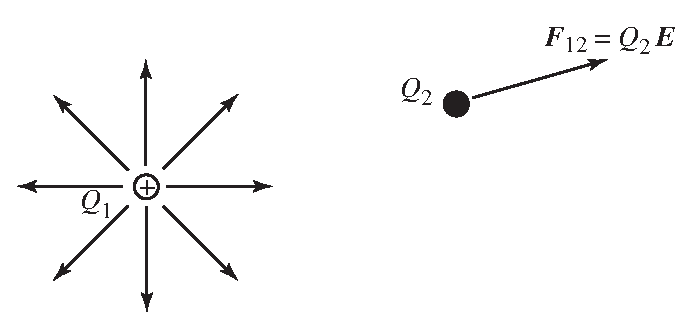
\epsfig{width=4.in,file=Figures/Em-review/coulomb.eps}
  \end{center}
  \caption{The force experienced by charge $Q_2$ due to charge $Q_1$ is
  along the line which pass through both charges.  The direction of
  the force is dictate by the signs of the charges.  Electric field is
  assumed to point radially away from positive charges as is indicated
  by the lines pointing away from $Q_1$ (which is assumed here to
  be positive).}
  \label{fig:coulomb}
\end{figure}
The force is proportional to the charges and inversely proportional to
the square of the distance between the charges.  A proportionality
constant is needed to obtain Coulomb's law which gives the equation of
the force on $Q_2$ due to $Q_1$:
\begin{equation}
  \mathbf{F}_{12} = \unitvec{12}
                    \frac{1}{4\pi\epsilon_0}
                    \frac{Q_1 Q_2}{R_{12}^2}
  \label{eq:coulomb}
\end{equation}
where $\unitvec{12}$ is a unit vector pointing from $Q_1$ to $Q_2$,
$R_{12}$ is the distance between the charges, and $1/4\pi\epsilon_0$
is the proportionality constant.  The constant $\epsilon_0$ is known
as the permittivity of free space and equals approximately
$8.854\times 10^{-12}$ F/m.  Charge is expressed in units of Coulombs
(C) and can be either negative or positive.  When the two charges have
like signs, the force will be repulsive: $\mathbf{F}_{12}$ will
be parallel to $\unitvec{12}$.  When the charges are of opposite sign,
the force will be attractive so that $\mathbf{F}_{12}$ will be
anti-parallel to $\unitvec{12}$.

There is a shortcoming with \refeq{eq:coulomb} in that it implies
action at a distance.  It appears from this equation that the force
$\mathbf{F}_{12}$ is established instantly.  From this equation one
could assume that a change in the distance $R_{12}$ results in an
instantaneous change in the force $\mathbf{F}_{12}$, but this is not
the case.  A finite amount of time is required to communicate the
change in location of one charge to the other charge (similarly, it
takes a finite amount of time to communicate a change in the quantity
of one charge to the other charge).  To overcome this shortcoming it
is convenient to employ the concept of fields.  Instead of $Q_1$
producing a force directly on $Q_2$, $Q_1$ is said to produce a field.
This field then produces a force on $Q_2$.  The field produced by
$Q_1$ is independent of $Q_2$---it exists whether or not $Q_2$ is
there to experience it.

In the static case, the field approach does not appear to have any
advantage over the direct use of Coulomb's law.  This is because for
static charges Coulomb's law is correct.  Fields must be time-varying
for the distinction to arise.  Nevertheless, to be consistent with the
time-varying case, fields are used in the static case as well.  The
electric field produced by the point charge $Q_1$ is
\begin{equation}
  \Evec_1 = \unitvec{r} \frac{Q_1}{4 \pi\epsilon_0 r^2}
  \label{eq:eField}
\end{equation}
where $\unitvec{r}$ is a unit vector which points radially away from
the charge and $r$ is the distance from the charge.  The electric
field has units of volts per meter (V/m).

To find the force on $Q_2$, one merely takes the charge times the
electric field: $\mathbf{F}_{12}=Q_2 \Evec_1$.  In general, the force
on any charge $Q$ is the product of the charge and the electric field
at which the charge is present, i.e., $\mathbf{F}=Q \Evec$.

\section{Electric Flux Density}

All material is made up of charged particles.  The material may be
neutral overall because it has as many positive charges as negative
charges.  Nevertheless, there are various ways in which the positive
and negative charges may shift slightly within the material, perhaps
under the influence of an electric field.  The resulting
charge separation will have an effect on the overall electric field.
Because of this it is often convenient to introduce a new field known
as the electric flux density, $\Dvec$, which has units of Coulombs per
square meter (C/m$^2$).\footnote{Note that not everybody advocates
using the $\Dvec$ field.  See for example Volume II of {\em The
Feynman Lectures on Physics}, R. P. Feynman, R. B. Leighton, and
M. Sands, Addison-Wesley, 1964.  Feynman only uses $\Evec$ and never
resorts to $\Dvec$.}  Essentially the $\Dvec$ field ignores the local
effects of charge which is bound in a material.

In free space, the electric field and the electric flux density are
related by
\begin{equation}
  \Dvec = \epsilon_0\Evec.
\end{equation}
Gauss's law states that
integrating $\Dvec$ over a closed surface yields the enclosed free
charge
\begin{equation}
  \oint_S \Dvec\cdot \mathbf{ds} = Q_{\mbox{\scriptsize enc}}
  \label{eq:gauss}
\end{equation}
where $S$ is the closed surface, $\mathbf{ds}$ is an incremental
surface element whose normal is directed radially outward, and
$Q_{\mbox{\scriptsize enc}}$ is the enclosed charge.  As an example,
consider the electric field given in \refeq{eq:eField}.  Taking $S$ to
be a spherical surface with the charge at the center, it is simple to
perform the integral in \refeq{eq:gauss}:
\begin{equation}
  \oint_S \Dvec\cdot \mathbf{ds} =
  \int_{\theta=0}^\pi\int_{\phi=0}^{2\pi}
    \epsilon_0 \frac{Q_1}{4 \pi\epsilon_0 r^2}\unitvec{r} \cdot
    \unitvec{r} r^2\sin\theta \, d\phi \, d\theta = Q_1.
  \label{eq:gaussExamp}
\end{equation}
The result is actually independent of the surface chosen (provided it
encloses the charge), but the integral is especially easy to perform
for a spherical surface.

We want the integral in \refeq{eq:gauss} always to equal the enclosed
charge as it does in free space.  However, things are more complicated
when material is present.  Consider, as shown in Fig.\
\ref{fig:platesFree}, two large parallel plates which carry uniformly
distributed charge of equal magnitude but opposite sign.  
\begin{figure}
  \begin{center}
  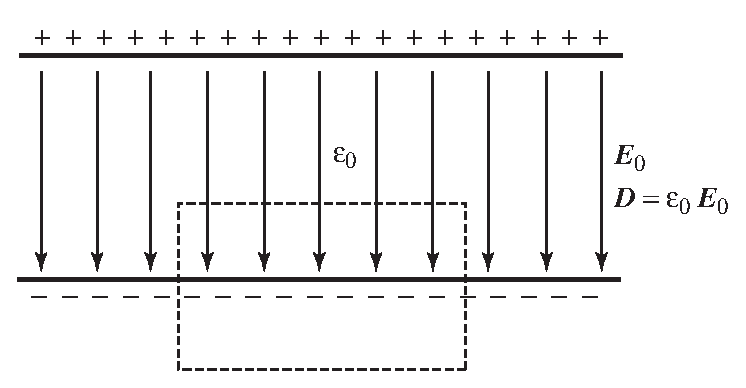
\epsfig{width=4.5in,file=Figures/Em-review/parallel-plates.eps}
  \end{center}
  \caption{Charged parallel plates in free space.  The dashed line
  represents the integration surface $S$.}
  \label{fig:platesFree}
\end{figure}
The dashed line represents an integration surface $S$ which is assumed
to be sufficiently far from the edges of the plate so that the field
is uniform over the top of $S$.  This field is identified as
$\Evec_0$.  The fields are zero outside of the plates and are
tangential to the sides of $S$ within the plates.  Therefore the only
contribution to the integral would be from the top of $S$.  The result
of the integral $\oint_S \epsilon_0\Evec\cdot \mathbf{ds}$ 
is the negative charge enclosed by the surface (i.e., the negative
charge on the bottom plate which falls within $S$).

Now consider the same plates, carrying the same charge, but with a
material present between the plates.  Assume this material is
``polarizable'' such that the positive and negative charges can shift
slightly.  The charges are not completely free to move---they are
bound charges.  The positive charges will be repelled by the top plate
and attracted to the bottom plate.  Conversely, the negative charges
will be repelled by the bottom plate and attracted to the top plate.
This scenario is depicted in Fig.\ \ref{fig:platesMat}.
\begin{figure}
  \begin{center}
  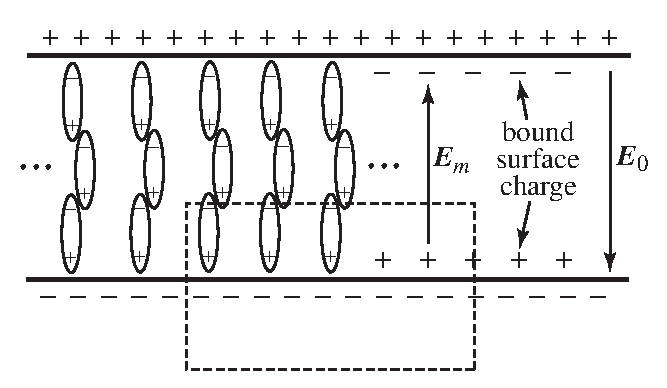
\epsfig{width=4.5in,file=Figures/Em-review/parallel-plates-dielectric.eps}
  \end{center} \caption{Charged parallel plates with a polarizable
  material present between the plates.  The elongated objects
  represent molecules whose charge orientation serves to produce a net
  bound negative charge layer at the top plate and a bound positive
  charge layer at the bottom plate.  In the interior, the positive and
  negative bound charges cancel each other.  It is only at the surface
  of the material where one must account for the bound charge.  Thus,
  the molecules are not drawn throughout the figure.  Instead, as
  shown toward the right side of the figure, merely the bound charge
  layer is shown.  The free charge on the plates creates the electric
  field $\Evec_0$.  The bound charge creates the electric field
  $\Evec_m$ which opposes $\Evec_0$ and hence diminishes the total
  electric field. The dashed line again represents the integration
  surface $S$.}  \label{fig:platesMat}
\end{figure}

With the material present the electric field due to the charge on the
plates is still $\Evec_0$, i.e., the same field as existed in Fig.\
\refeq{fig:platesFree}.  However, there is another field present due
to the displacement of the bound charge in the polarizable material
between the plates.  The polarized material effectively acts to
establish a layer of positive charge adjacent to the bottom plate and
a layer of negative charge adjacent to the top plate.  The field due
to these layers of charge is also uniform but it is in the opposite
direction of the field caused by the ``free charge'' on the plates.
The field due to bound charge is labeled $\Evec_m$ in Fig.\
\refeq{fig:platesMat}.  The total field is the sum of the fields due
to the bound and free charges, i.e., $\Evec = \Evec_0 + \Evec_m$.
Because $\Evec_0$ and $\Evec_m$ are anti-parallel, the magnitude of
the total electric field $\Evec$ will be less than $\Evec_0$.

Since the material is neutral, we would like the integral of the
electric flux over the surface $S$ to yield just the enclosed charge
on the bottom plate---not the bound charge due to the material.  In
some sense this implies that the integration surface cannot separate
the positive and negative bound charge of any single molecule.  Each
molecule is either entirely inside or outside the integration surface.
Since each molecule is neutral, the only contribution to the integral
will be from the free charge on the plate.

With the material present, the integral of $\oint_S
\epsilon_0\Evec\cdot \mathbf{ds}$ yields too little charge.  This is
because, as stated above, the total electric field $\Evec$ is less
than it would be if only free space were present.  To correct for the
reduced field and to obtain the desired result, the electric flux
density is redefined so that it accounts for the presence of the
material.  The more general expression for the electric flux density
is
\begin{equation}
 \Dvec = \epsilon_r\epsilon_0\Evec = \epsilon\Evec
 \label{eq:eAndD}
\end{equation}
where $\epsilon_r$ is the relative permittivity and $\epsilon$ is
called simply the permittivity.  By accounting for the permittivity of
a material, Gauss's law is always satisfied.

In \refeq{eq:eAndD}, $\Dvec$ and $\Evec$ are related by a scalar
constant.  This implies that the $\Dvec$ and $\Evec$ fields are
related by a simple proportionality constant for all frequencies, all
orientations, and all field strengths.  Unfortunately the real world
is not so simple.  Clearly if the electric field is strong enough, it
would be possible to tear apart the bound positive and negative
charges.  Since charges have some mass, they do not react the same way
at all frequencies.  Additionally, many materials may have some
structure, such as crystals, where the response in one direction is
not the same in other directions.  Nevertheless, Gauss's law is the
law and thus always holds.  When things get more complicated one must
abandon a simple scalar for the permittivity and use an appropriate
form to ensure Gauss's law is satisfied.  So, for example, it may be
necessary to use a tensor for permittivity that is directionally
dependent.  However, with the exception of frequency-dependent
behavior (i.e., dispersive materials), we will not be pursuing those
complications.  A scalar permittivity will suffice.

\section{Static Electric Fields}

Ignoring possible nonlinear behavior of material, superposition holds
for electromagnetic fields.  Therefore we can think of any
distribution of charges as a collection of point charges.  We can get
the total field by summing the contributions from all the charges (and
this summing will have to be in the form of an integration if the
charge is continuously distributed).

Note from \refeq{eq:eField} that the field associated with a point
charge merely points radially away from the charge.  There is no
``swirling'' of the field.  If we have more than a single charge, the
total field may bend, but it will not swirl.  Imagine a tiny wheel
with positive charge distributed around its circumference.  The wheel
hub of the wheel is held at a fixed location but the wheel is free to
spin about its hub.  For static electric fields, no matter where we
put this wheel, there would be no net force on the wheel to cause it
to spin.  There may be a net force pushing the entire wheel in a
particular direction (a translational force), but the forces which are
pushing the wheel to spin in the clockwise direction are balanced by
the forces pushing the wheel to spin in the counterclockwise
direction.

Another property of electrostatic fields is that the electric flux
density only begins or terminates on free charge.  If there is no
charge present, the lines of flux continue.

The lack of swirl in the electric field and the source of electric
flux density are fairly simple concepts.  However, to be able to
analyze the fields properly, one needs a mathematical statement of
these concepts.  The appropriate statements are
\begin{equation}
  \nabla\times\Evec=0
  \label{eq:curlE}
\end{equation}
and
\begin{equation}
  \nabla\cdot\Dvec=\rho_v
  \label{eq:divD}
\end{equation}
where $\nabla$ is the del or nabla operator and $\rho_v$ is the
electric charge density (with units of C/m$^3$).  Equation
\refeq{eq:curlE} is the curl of the electric field and \refeq{eq:divD}
is the divergence of the electric flux density.  These two equations
are discussed further in the following section.

\section{Gradient, Divergence, and Curl}

The del operator is independent of the coordinate system
used---naturally the behavior of the fields should not depend on the
coordinate system used to describe the field.  Nevertheless, the del
operator can be expressed in different coordinates systems.  In
Cartesian coordinates del is
\begin{equation}
  \nabla \equiv \unitvec{x} \frac{\partial}{\partial x} +
                \unitvec{y} \frac{\partial}{\partial y} +
                \unitvec{z} \frac{\partial}{\partial z}
\end{equation}
where the symbol $\equiv$ means ``defined as.''

Del acting on a scalar field produces the gradient of the field.
Assuming $f$ is a some scalar field, $\nabla f$ produces the vector
field given by 
\begin{equation}
  \nabla f = \unitvec{x} \frac{\partial f}{\partial x} +
             \unitvec{y} \frac{\partial f}{\partial y} +
             \unitvec{z} \frac{\partial f}{\partial z}.
\end{equation}
The gradient of $f$ points in the direction of greatest change and is
proportional to the rate of change.  Assume we wish to find the amount
of change in $f$ for a small movement $dx$ in the $x$ direction.  This
can be obtained via $\nabla f \cdot \unitvec{x} dx$, to wit
\begin{equation}
  \nabla f \cdot \unitvec{x} dx = \frac{\partial f}{\partial x} dx
    = \mbox{(rate of change in $x$ direction)}\times
      \mbox{(movement in $x$ direction)}.
\end{equation}
This can be generalized for movement in an arbitrary direction.
Letting an incremental small length be given by
\begin{equation}
  \mathbf{d\ell} = \unitvec{x} dx + \unitvec{y} dy + \unitvec{z} dz,
\end{equation}
the change in the field realized by moving an amount $\mathbf{d\ell}$
is
\begin{equation}
  \nabla f\cdot\mathbf{d\ell} = 
     \frac{\partial f}{\partial x} dx +
     \frac{\partial f}{\partial y} dy +
     \frac{\partial f}{\partial z} dz.
\end{equation}

Returning to \refeq{eq:divD}, when the del operator is dotted with a
vector field, one obtains the divergence of that field.  Divergence
can be thought of as a measure of ``source'' or ``sink'' strength of the
field at a given point.  The divergence of a vector field is a scalar
field given by
\begin{equation}
 \nabla \cdot \Dvec = \frac{\partial D_x}{\partial x} +
     \frac{\partial D_y}{\partial y} +
     \frac{\partial D_z}{\partial z}.
\end{equation}
Let us consider a finite-difference approximation of this divergence
in the $xy$-plane as shown in Fig.\ \ref{fig:div}.
\begin{figure}
  \begin{center}
  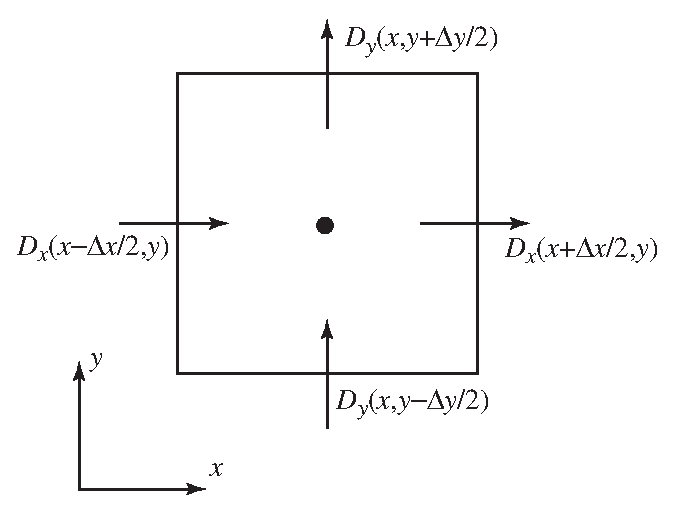
\epsfig{width=3.5in,file=Figures/Em-review/discrete-divergence.eps}
  \end{center}
  \caption{Discrete approximation to the divergence taken in the
  $xy$-plane. \label{fig:div}}  
\end{figure}
Here the divergence is measured over a small box where the field is
assumed to be constant over each edge of the box.  The derivatives can
be approximated by central differences:
\begin{equation}
  \frac{\partial D_x}{\partial x} +
  \frac{\partial D_y}{\partial y} \approx 
  \frac{D_x\left(x+\frac{\Delx}{2},y\right)
       -D_x\left(x-\frac{\Delx}{2},y\right)}{\Delx} +
  \frac{D_y\left(x,y+\frac{\Dely}{2}\right)
       -D_y\left(x,y-\frac{\Dely}{2}\right)}{\Dely}
  \label{eq:divII}
\end{equation}
where this is exact as $\Delx$ and $\Dely$ go to zero.
Letting $\Delx=\Dely=\delta$, \refeq{eq:divII} can be written
\begin{equation}
  \frac{\partial D_x}{\partial x} +
  \frac{\partial D_y}{\partial y} \approx 
  \frac{1}{\delta}
  \left(D_x\left(x+\frac{\delta}{2},y\right) -
        D_x\left(x-\frac{\delta}{2},y\right) +
        D_y\left(x,y+\frac{\delta}{2}\right) -
        D_y\left(x,y-\frac{\delta}{2}\right)\right).
  \label{eq:divIII}
\end{equation}
Inspection of \refeq{eq:divIII} reveals that the divergence is
essentially a sum of the field over the faces with the appropriate
sign changes.  Positive signs are used if the field is assumed to
point out of the box and negative signs are used when the field is
assumed to point into the box.  If the sum of these values is
positive, that implies there is more flux out of the box than into it.
Conversely, if the sum is negative, that means more flux is flowing
into the box than out.  If the sum is zero, there must be as much flux
flowing into the box as out of it (that does not imply necessarily that,
for instance, $D_x\left(x+\delta/2,y\right)$ is equal to
$D_x\left(x-\delta/2,y\right)$, but rather that the sum of all four
fluxes must be zero).

Equation \refeq{eq:divD} tells us that the electric flux density has
zero divergence except where there is charge present (as specified by
the charge-density term $\rho_v$).  If the charge density is zero, the
total flux entering some small enclosure must also leave it.  If the
charge density is positive at some point, more flux will leave a small
enclosure surrounding that point than will enter it.  On the other
hand, if the charge density is negative, more flux will enter the
enclosure surrounding that point than will leave it.

Finally, let us consider \refeq{eq:curlE} which is the curl of the
electric field.  In Cartesian coordinates it is possible to treat this
operation as simply the cross product between the vector operator
$\nabla$ and the vector field $\Evec$:
\begin{equation}
  \nabla\times\Evec =
  \left|
  \begin{array}{ccc}
     \unitvec{x} & \unitvec{y} & \unitvec{z} \\
     \frac{\partial}{\partial x} &
     \frac{\partial}{\partial y} &
     \frac{\partial}{\partial z} \\
     E_x & E_y & E_z
  \end{array}
  \right|
  =
  \unitvec{x}\left(\frac{\partial E_z}{\partial y} -
                   \frac{\partial E_y}{\partial z}\right) +
  \unitvec{y}\left(\frac{\partial E_x}{\partial z} -
                   \frac{\partial E_z}{\partial x}\right) +
  \unitvec{z}\left(\frac{\partial E_y}{\partial x} -
                   \frac{\partial E_x}{\partial y}\right).
  \label{eq:curl}
\end{equation}
Let us consider the behavior of only the $z$ component of this
operator which is dictated by the field in the $xy$-plane as shown in
Fig.\ \ref{fig:curl}.
\begin{figure}
  \begin{center}
  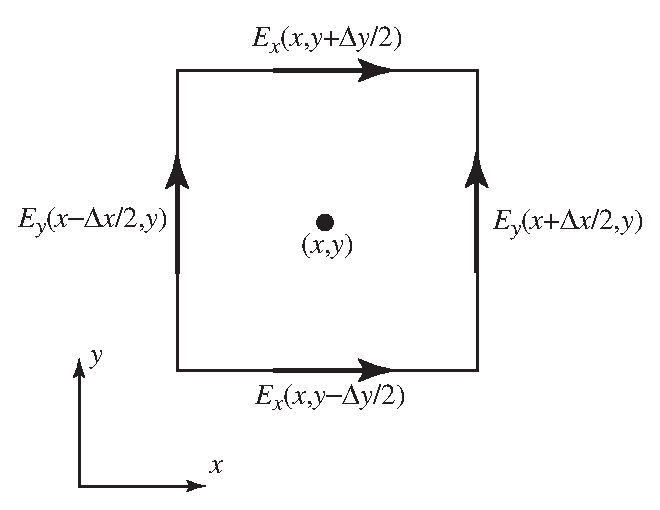
\epsfig{width=3.5in,file=Figures/Em-review/discrete-curl.eps}
  \end{center}
  \caption{Discrete approximation to the curl taken in the
  $xy$-plane. \label{fig:curl}}
\end{figure}
The $z$-component of $\nabla\times\Evec$ can be written as
\begin{equation}
  \frac{\partial E_y}{\partial x} -
  \frac{\partial E_x}{\partial y} \approx 
  \frac{E_y\left(x+\frac{\Delx}{2},y\right)
       -E_y\left(x-\frac{\Delx}{2},y\right)}{\Delx} -
  \frac{E_x\left(x,y+\frac{\Dely}{2}\right)
       -E_x\left(x,y-\frac{\Dely}{2}\right)}{\Dely}.
  \label{eq:curlII}
\end{equation}
The finite-difference approximations of the derivatives are again
based on the fields on the edges of a box surrounding the point of
interest.  However, in this case the relevant fields are tangential to
the edges rather than normal to them.  Again letting
$\Delx=\Dely=\delta$, \refeq{eq:curlII} can be written
\begin{equation}
  \frac{\partial E_y}{\partial x} -
  \frac{\partial E_x}{\partial y} \approx 
  \frac{1}{\delta}
  \left(E_y\left(x+\frac{\delta}{2},y\right) -
        E_y\left(x-\frac{\delta}{2},y\right) -
        E_x\left(x,y+\frac{\delta}{2}\right) +
        E_x\left(x,y-\frac{\delta}{2}\right)\right).
  \label{eq:curlIII}
\end{equation}
In the sum on the right side the sign is positive if the vector
component points in the counterclockwise direction (relative to
rotations about the center of the box) and is negative if the vector
points in the clockwise direction.  Thus, if the sum of these vector
components is positive, that implies that the net effect of these
electric field vectors is to tend to push a positive charge in the
counterclockwise direction.  If the sum were negative, the vectors
would tend to push a positive charge in the clockwise direction.  If
the sum is zero, there is no tendency to push a positive charge around
the center of the square (which is not to say there would not be a
translation force on the charge---indeed, if the electric field is
non-zero, there has to be some force on the charge).

\section{Laplacian}

In addition to the gradient, divergence, and curl, there is one more
vector operator to consider.  There is a vector identity that the curl
of the gradient of any function is identically zero
\begin{equation}
  \nabla\times\nabla f = 0.
  \label{eq:vecIdent}
\end{equation}
This is simple to prove by merely performing the operations in
Cartesian coordinates.  One obtains several second-order partial
derivatives which cancel if the order of differentiation is switched.
Recall that for a static distribution of charges, $\nabla\times\Evec=0$.
Since the curl of the electric field is zero, it should be possible to
represent the electric field as the gradient of some scalar function
\begin{equation}
  \Evec = -\nabla V.
  \label{eq:potential}
\end{equation}
The scalar function $V$ is the electric potential and the negative
sign is used to make the electric field point from higher potential to
lower potential (by historic convention the electric field points away
from positive charge and toward negative charge).  By expressing the
electric field this way, the curl of the electric field is guaranteed
to be zero.

Another way to express the relationship between the electric field and
the potential is via integration.  Consider movement from an arbitrary
point $a$ to an arbitrary point $b$.  The change in potential between
these two points can be expressed as
\begin{equation}
  V_b-V_a = \int_a^b \nabla V \cdot \mathbf{d\ell}.
  \label{eq:potentialInt}
\end{equation}
The integrand represent the change in the potential for a movement
$\mathbf{d\ell}$ and the integral merely sums the changes over the
path from $a$ to $b$.  However, the change in potential must also be
commensurate with the movement in the direction of, or against, the
electric field.  If we move against the electric field, potential
should go up.  If we move along the electric field, the potential
should go down.  In other words, the incremental change in potential
for a movement $\mathbf{d\ell}$ should be
$dV=-\Evec\cdot\mathbf{d\ell}$ (if the movement $\mathbf{d\ell}$ is
orthogonal to the electric field, there should be no change in the
potential).  Summing change in potential over the entire path yields
\begin{equation}
  V_b-V_a = - \int_a^b \Evec \cdot \mathbf{d\ell}.
  \label{eq:potentialIntII}
\end{equation}
The integrals in \refeq{eq:potentialInt} and \refeq{eq:potentialIntII}
can be equated.  Since the equality holds for any two arbitrary points,
the integrands must be equal and we are again left with $\Evec =
-\nabla V$. 

The electric flux density can be related to the electric field via
$\Dvec=\epsilon\Evec$ and the behavior of the flux density $\Dvec$ is
dictated by $\nabla\cdot\Dvec=\rho_v$.  Combining these with
\refeq{eq:potential} yields
\begin{equation}
  \Evec = \frac{1}{\epsilon}\Dvec = -\nabla V.
\end{equation}
Taking the divergence of both sides yields
\begin{equation}
  \frac{1}{\epsilon}\nabla\cdot\Dvec =  
  \frac{1}{\epsilon} \rho_v =
  -\nabla\cdot\nabla V.
\end{equation}
Rearranging this yields Poisson's equation given by
\begin{equation}
  \nabla^2 V = -\frac{\rho_v}{\epsilon}
  \label{eq:poisson}
\end{equation}
where $\nabla^2$ is the Laplacian operator
\begin{equation}
  \nabla^2 \equiv \nabla\cdot\nabla =
     \frac{\partial^2}{\partial x^2} +
     \frac{\partial^2}{\partial y^2} +
     \frac{\partial^2}{\partial z^2}.
\end{equation}
Note that the Laplacian is a scalar operator.  It can act on a scalar
field (such as the potential $V$ as shown above) or it can act on a
vector field as we will see later.  When it acts on a vector field,
the Laplacian acts on each component of the field.

In the case of zero charge density, \refeq{eq:poisson} reduces to
Laplace's equation
\begin{equation}
  \nabla^2 V = 0.
\end{equation}  
We have a physical intuition about what gradient, divergence, and curl
are telling us, but what about the Laplacian?  To answer this,
consider a function of a single variable.

Given the function $V(x)$, we can ask if the function at some point is
greater than, equal to, or less than the average of its neighboring
values.  The answer can be expressed in terms of the value of the
function at the point of interest and the average of samples to either
side of that central point:
\begin{equation}
  \frac{V(x+\delta) + V(x-\delta)}{2} - V(x) =
  \left\{
    \begin{array}{ll}
      \mbox{positive}&\mbox{if center point less than average of neighbors} \\
      \mbox{zero} &\mbox{if center point equals average of neighbors} \\
      \mbox{negative}&\mbox{if center point greater than average of neighbors}
    \end{array}
  \right.
  \label{eq:avg}
\end{equation}
Here the left-most term represents the average of the neighboring
values and $\delta$ is some displacement from the central point.
Equation \refeq{eq:avg} can be normalized by $\delta^2/2$ without changing
the basic tenants of this equation.  Performing that normalization and
rearranging yields
\begin{eqnarray}  
  \frac{1}{\delta^2/2}
  \left\{
    \frac{V(x+\delta) + V(x-\delta)}{2} - V(x)
  \right\}
  &=&
  \frac{1}{\delta^2}
  \left\{
    (V(x+\delta) - V(x)) - (V(x)-V(x-\delta))
  \right\} \nonumber
 \\
  &=&
  \frac{
    \frac{V(x+\delta) - V(x)}{\delta} -
    \frac{V(x)-V(x-\delta)}{\delta}}{\delta}  \nonumber
 \\
  &\approx&
  \frac{
    \frac{\partial V(x+\delta/2)}{\partial x} -
    \frac{\partial V(x-\delta/2)}{\partial x}}{\delta} \nonumber
 \\
  &\approx&
  \frac{\partial^2 V(x)}{\partial x^2}.
\end{eqnarray}
Thus the second partial derivative can be thought of as a way of
measuring the field at a point relative to its neighboring points.
You should already have in mind that if the second derivative is
negative, a function is tending to curve downward.  Second derivatives
are usually discussed in the context of curvature.  However, you
should also think in terms of the field at a point and its neighbors.
At points where the second derivative is negative those points are
higher than the average of their neighboring points (at least if the
neighbors are taken to be an infinitesimally small distance away).

In lieu of these arguments, Poisson's equation \refeq{eq:poisson}
should have physical significance.  Where the charge density is zero,
the potential cannot have a local minima or maxima.  The potential is
always equal to the average of the neighboring points.  If one
neighbor is higher, the other must be lower (and this concept easily
generalizes to higher dimensions).  Conversely, if the charge density
is positive over some region, the potential should increase as one
moves deeper into that region but the rate of increase must be such
that at any point the average of the neighbors is less than the center
point.  This behavior is illustrated in Fig.\ \ref{fig:chargeSphere}
which depicts the potential along a path through the center of a
uniform sphere of charge.
\begin{figure}
  \begin{center}
  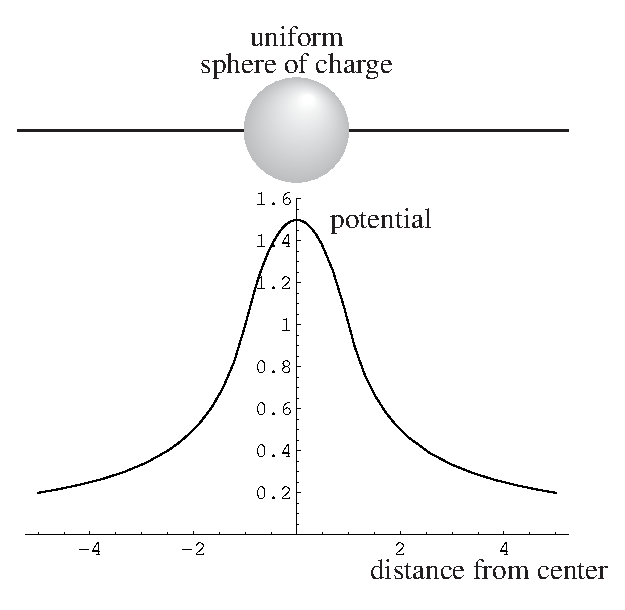
\epsfig{width=4in,file=Figures/Em-review/sphere-potential.eps}
  \end{center}
  \caption{Potential along a path which passes through a uniform
  sphere of positive charge (arbitrary units). \label{fig:chargeSphere}}
\end{figure}

\section{Gauss's and Stokes' Theorems}

Equation \refeq{eq:gauss} presented Gauss's law which stated the flux
of $\Dvec$ through a closed surface $S$ is equal to the enclosed
charge.  There is an identity in vector calculus, known as Gauss's
theorem, which states that the integral of the flux of any vector
field through a closed surface equals the integral of the divergence
of the field over the volume enclosed by the surface.  This holds for
any vector field, but using the $\Dvec$ field, Gauss's theorem states
\begin{equation}
  \oint_S \Dvec\cdot\mathbf{ds} = 
  \int_V \nabla\cdot \Dvec dv
  \label{eq:gaussTheorem}
\end{equation}
where $V$ is the enclosed volume and $dv$ is a differential volume
element.  Note that the left-hand side of \refeq{eq:gaussTheorem} is
the left-hand side of \refeq{eq:gauss}.

The right-hand side of \refeq{eq:gauss} is the enclosed charge
$Q_{\mbox{\scriptsize enc}}$ which could be determined either by
evaluating the left-hand side of \refeq{eq:gauss} or by integration of
the charge density $\rho_v$ over the volume enclosed by $S$.  (This is
similar to determining the mass of an object by integrating its mass
density over its volume.)  Thus,
\begin{equation}
  Q_{\mbox{\scriptsize enc}} =
  \int_V \rho_v dv.
  \label{eq:chargeIntegral}
\end{equation}
Equating the right-hand sides of \refeq{eq:gaussTheorem} and
\refeq{eq:chargeIntegral} yields
\begin{equation}
  \int_V \nabla\cdot \Dvec dv =
  \int_V \rho_v dv.
\end{equation}
Since this must hold over an arbitrary volume, the integrands must be
equal which yields \refeq{eq:divD}.

Another useful identity from vector calculus is Stokes' theorem which
states that the integral of a vector field over any closed path is
equal to the integral of the curl of that field over a surface which
has that path as its border.  Again, this holds for any vector field,
but using the electric field as an example one can write
\begin{equation}
  \oint_L \Evec\cdot\mathbf{d\ell} = 
  \int_S \nabla\times\Evec \cdot \mathbf{ds}.
  \label{eq:stokes}
\end{equation}
The surface normal is assumed to follow the right-hand convention so
that when the fingers of the right hand are oriented along the path of
the loop, the thumb points in the positive direction of the surface
normal.

Static electric fields are conservative which means that the net work
required to move a charge in a closed path is always zero.  Along some
portion of the path positive work would have to be done to push the
charge against the field, but this amount of work would be given back
by the field as the charge travels along the remaining portions of the
path.  The integrand on the left-hand side in \refeq{eq:stokes} is the
field dotted with an incremental length.  If the integrand were
multiplied by a unit positive charge, the integrand would represent
work, since charge times field is force and force times distance is
work.  Because the electric field is conservative, the integral on the
left-hand side of \refeq{eq:stokes} must be zero.  Naturally this
implies that the integral on the right-hand side must also be zero.
Since this holds for any loop $L$ (or, similarly, any surface $S$), the
integrand itself must be zero.  Equating the integrand to zero yields
\refeq{eq:curlE}.

\section{Electric Field Boundary Conditions}

Consider an interface between two homogeneous regions.  Because
electric flux density only begins or ends on charge, the normal
component of $\Dvec$ can only change at the interface if there is
charge on the interface, i.e., surface charge is present.  This can be
stated mathematically as
\begin{equation}
 \hat{\mathbf{n}} \cdot(\Dvec_1 - \Dvec_2) = \rho_s
\end{equation}
where $\rho_s$ is a surface charge density (C/m$^2$),
$\hat{\mathbf{n}}$ is a unit vector normal to the surface, and
$\Dvec_1$ and $\Dvec_2$ are the field to either side of the interface.
One should properly argue this boundary condition by an application of
Gauss's law for a small volume surrounding the surface, but such
details are left to other classes (this is just a review!).  If no
charge is present, the normal components must be equal
\begin{equation}
 \hat{\mathbf{n}} \cdot \Dvec_1 = \hat{\mathbf{n}} \cdot \Dvec_2.
\end{equation}

The boundary conditions on the tangential component of the electric
field can be determined by integrating the electric field over a
closed loop which is essentially a rectangle which encloses a portion
of the interface.  By letting the sides shrink to zero and keeping the
``top'' and ``bottom'' of the rectangle small but finite (so that they
are tangential to the surface), one essentially has that the field
over the top must be the same as the field over the bottom (owing to
the fact that total integral must be zero since the field is
conservative).  Stated mathematical, the boundary condition is
\begin{equation}
 \hat{\mathbf{n}} \times (\Evec_1 - \Evec_2) = 0.
\end{equation}

\section{Conductivity and Perfect Electric Conductors}

It is possible for the charge in materials to move under the influence
of an electric field such that currents flow.  If the material has a
non-zero conductivity $\sigma$, the current density is given by
\begin{equation}
  \Jvec = \sigma \Evec.
\end{equation}
The current density has units of A/m$^2$ and the conductivity has
units of S/m.

If charge is building up or decaying in a particular region, the
divergence of the current density must be non-zero.  If the divergence
is zero, that implies as much current leaves a point as enters it and
there is no build-up or decay of charge.  This can be stated as
\begin{equation}
  \nabla \cdot \Jvec = -\frac{\partial \rho_v}{\partial t}.
  \label{eq:chargeConservation}
\end{equation}
If the divergence is positive, the charge density must be decreasing
with time (so the negative sign will bring the two into agreement).
This equation is a statement of charge conservation.

Perfect electric conductors (PECs) are materials where it is assumed
that the conductivity approaches infinity.  If the fields were
non-zero in a PEC, that would imply the current was infinite.  Since
infinite currents are not allowed, the fields inside a PEC are
required to be zero.  This subsequently requires that the tangential
electric field at the surface of a PEC is zero (since tangential
fields are continuous across an interface and the fields inside the
PEC are zero).  Correspondingly, the normal component of the electric
flux density $\Dvec$ at the surface of a PEC must equal the charge
density at the surface of the PEC.  Since the fields inside a PEC are
zero, all points of the PEC must be at the same potential.

\section{Magnetic Fields}

Magnetic fields circulate around, but they do not terminate on
anything---there is no (known) magnetic charge.  Nevertheless, it is
often convenient to define magnetic charge and magnetic current.
These fictions allow one to simplify various problems such as integral
formulations of scattering problems.  However for now we will stick to
reality and say they do not exist.

The magnetic flux density $\Bvec$ is somewhat akin to the electric
field in that the force on a charge in motion is related to $\Bvec$.
If a charge $Q$ is moving with velocity $\mathbf{u}$ in a field
$\Bvec$, it experiences a force
\begin{equation}
  \mathbf{F} = Q \mathbf{u}\times\Bvec.
\end{equation}
Because $\Bvec$ determines the force on a charge, it must account for
all sources of magnetic field.  When material is present, the charge
in the material can have motion (or rotation) which influences the
magnetic flux density.

Alternatively, similar to the electric flux density, we define the
magnetic field $\Hvec$ which ignores the local effects of material.
These fields are related by
\begin{equation}
  \Bvec = \mu_r\mu_0 \Hvec = \mu\Hvec
\end{equation}
where $\mu_r$ is the relatively permeability, $\mu_0$ is the
permeability of free space equal to $4\pi\times 10^{-7}$ H/m, and
$\mu$ is simply the permeability.  Typically the relative permeability
is greater than unity (although usually only by a small amount) which
implies that when a material is present the magnetic flux density is
larger than when there is only free space.

Charge in motion is the source of magnetic fields.  If a current $I$
flows over an incremental distance $\mathbf{d\ell}$, it will produce a
magnetic field given by:
\begin{equation}
  \Hvec = \frac{I\mathbf{d\ell}\times \mathbf{a}_r}
               {4 \pi r^2}
  \label{eq:biot}
\end{equation}
where $\mathbf{a}_r$ points from the location of the filament of
current to the observation point and $r$ is the distance between the
filament and the observation point.  Equation \refeq{eq:biot} is known
as the Biot-Savart equation.  Of course, because of the conservation
of charge, a current cannot flow over just a filament and then
disappear.  It must flow along some path.  Thus, the magnetic field
due to a loop of current would be given by
\begin{equation}
  \Hvec = \oint_L\frac{I\mathbf{d\ell}\times \mathbf{a}_r}
               {4 \pi r^2}.
  \label{eq:biotIntegral}
\end{equation}
If the current was flowing throughout a volume or over a surface, the
integral would be correspondingly changed to account for the
current wherever it flowed.

From \refeq{eq:biotIntegral} one sees that currents (which are just
another way of saying charge in motion) are the source of magnetic
fields.  Because of the cross-product in \refeq{eq:biot} and
\refeq{eq:biotIntegral}, the magnetic field essentially swirls around
the current.  If one integrates the magnetic field over a closed path,
the result is the current enclosed by that path
\begin{equation}
  \oint_L \Hvec \cdot \mathbf{d\ell} = I_{\mbox{\scriptsize enc}}.
  \label{eq:hIntegral}
\end{equation}
The enclosed current $I_{\mbox{\scriptsize enc}}$ is the current that
passes through the surface $S$ which is bound by the loop $L$.

The left-hand side of \refeq{eq:hIntegral} can be converted to a
surface integral by employing Stokes' theorem while the right-hand
side can be related to the current density by integrating over the
surface of the loop.  Thus,
\begin{equation}
  \oint_L \Hvec\cdot \mathbf{d\ell} = 
  \int_S \nabla\times\Hvec \cdot \mathbf{ds} =
  I_{\mbox{\scriptsize enc}} =
  \int_S \Jvec \cdot \mathbf{ds}.
  \label{eq:hIntegralII}
\end{equation}
Since this must be true for every loop (and surface), the integrands
of the second and fourth terms can be equated.  This yields
\begin{equation}
  \nabla\times\Hvec = \Jvec.
\end{equation}

The last equation needed to characterize static fields is
\begin{equation}
  \nabla\cdot\Bvec=0.
\end{equation}
This is the mathematical equivalent of saying there is no magnetic
charge.

\section{Magnetic Field Boundary Conditions}

Note that the equation governing $\Bvec$ is similar to the equation
which governed $\Dvec$.  In fact, since the right-hand side is always
zero, the equation for $\Bvec$ is simpler.  The arguments used to
obtain the boundary condition for the normal component of the $\Dvec$
field can be applied directly to the $\Bvec$ field.  Thus, 
\begin{equation}
 \hat{\mathbf{n}} \cdot(\Bvec_1 - \Bvec_2) = 0.
\end{equation}

For the magnetic field, an integration path is constructed along
the same lines as the one used to determine the boundary condition on
the electric field.  Note that the equations governing $\Evec$ and
$\Hvec$ are similar except that the one for $\Hvec$ has a non-zero
right-hand side.  If the current density is zero over the region of
interest, then there is really no distinction between the two and one
can say that the tangential magnetic fields must be equal across a
boundary.  However, if a surface current exists on the interface,
there may be a discontinuity in the tangential fields.  The boundary
condition is given by
\begin{equation}
 \hat{\mathbf{n}} \times (\Hvec_1 - \Hvec_2)
  = \mathbf{K}
\end{equation}
where $\mathbf{K}$ is the surface current density (with units of A/m).


\section{Summary of Static Fields}

When a system is not changing with respect to time, the governing
equations are
\begin{eqnarray}
  \nabla \cdot \Dvec &=& \rho_v, \\
  \nabla \cdot \Bvec &=& 0, \\
  \nabla \times \Evec &=& 0, \\
  \nabla \times \Hvec &=& \Jvec. \label{eq:curlHdc}
\end{eqnarray}
If a loop carries a current but is otherwise neutral, it will produce
a magnetic field and only a magnetic field.  If a charge is
stationary, it will produce an electric field and only an electric
field.  The charge will not ``feel'' the loop current and the current
loop will not feel the stationary charge (at least approximately).
The magnetic field and electric field are decoupled.  If a charge $Q$
moves with velocity $\mathbf{u}$ in the presence of both an electric
field and a magnetic field, the force on the charge is the sum of the
forces due to the electric and magnetic fields
\begin{equation}
  \mathbf{F} = Q(\Evec + \mathbf{u}\times\Bvec).
\end{equation}

\section{Time Varying Fields}

What happens when a point charge moves?  We know that charge in motion
gives rise to a magnetic field, but if the charge is moving, its
associated electric field must also be changing.  Thus, when a system
is time-varying the electric and magnetic fields must be coupled.

There is a vector identity that the divergence of the curl of any
vector field is identically zero.  Taking the divergence of both sides
of \refeq{eq:curlHdc} yields
\begin{equation}
  \nabla\cdot \nabla \times \Hvec = 
  \nabla\cdot \Jvec =
  -\frac{\partial\rho_v}{\partial t}
\end{equation}
where the conservation of charge equation was used to write the last
equality.  Since the first term must be zero, this implies that 
$\partial\rho_v/\partial t$ must also be zero.  However, that
is overly restrictive.  In general, for a time-varying system, the
charge density will change with respect to time.  Therefore something
must be wrong with \refeq{eq:curlHdc} as it pertains to time-varying
fields.  It was Maxwell who recognized that by adding the temporal
derivative of the electric flux density to the right-hand side of
\refeq{eq:curlHdc} the equation would still be valid for the
time-varying case.  The correct equation is given by
\begin{equation}
  \nabla \times \Hvec = \Jvec + \frac{\partial \Dvec}{\partial t}
  \label{eq:curlHac}
\end{equation}
The term $\partial \Dvec/\partial t$ is known as the displacement
current while $\Jvec$ is typically called the conduction current.
Equation \refeq{eq:curlHac} is known as Ampere's law.

Taking the divergence of the right-hand side of \refeq{eq:curlHac}
yields
\begin{equation}
  \nabla\cdot\Jvec + \frac{\partial \nabla\cdot\Dvec}{\partial t} = 
  -\frac{\partial \rho_v}{\partial t} + 
    \frac{\partial \nabla\cdot\Dvec}{\partial t} = 
  -\frac{\partial \rho_v}{\partial t} + 
    \frac{\partial \rho_v}{\partial t}
  =  0
\end{equation}
where use was made of \refeq{eq:divD} and the conservation of charge
equation \refeq{eq:chargeConservation}.

The electromotive force (EMF) is the change in potential over some
path.  It has been observed experimentally that when a magnetic field
is time-varying there is a non-zero EMF over a closed path which
encloses the varying field (i.e., the electric field is no longer
conservative).  

The symbol $\lambda$ is often use to represent total magnetic flux
through a given surface, i.e.,
\begin{equation}
  \lambda = \int_S \Bvec\cdot\mathbf{ds}.
\end{equation}
For time-varying fields, the EMF over a closed path $L$ can be written
\begin{eqnarray}
  V_{\mbox{\scriptsize emf}} &=& \frac{d\lambda}{dt}, \\
  -\oint_L \Evec\cdot\mathbf{d\ell} &=& 
    \frac{d}{dt}\int_S \Bvec\cdot\mathbf{ds}, \\
  -\int_S \nabla\times\Evec\cdot\mathbf{ds} &=& 
    \int_S \frac{\partial\Bvec}{\partial t}\cdot\mathbf{ds},
\end{eqnarray}
where Stokes' theorem was used to write the last equation.  Since this
equality holds over any surface, the integrands must be equal.  This
yields
\begin{equation}
  \nabla\times\Evec = -\frac{\partial\Bvec}{\partial t}
\end{equation}
which is known as Faraday's law.

\section{Summary of Time-Varying Fields}

When a system is changing with respect to time, the governing
equations are
\begin{eqnarray}
\nabla \cdot \Dvec &=& \rho_v, \label{eq:divDtime} \\
\nabla \cdot \Bvec &=& 0, \\
\nabla \times \Evec &=& -\frac{\partial\Bvec}{\partial t}, 
  \label{eq:curlBtime} \\
\nabla \times \Hvec &=& \Jvec + \frac{\partial\Dvec}{\partial t}.
  \label{eq:curlHtime}
\end{eqnarray}
Note that the divergence equations are unchanged from the static
case.  The two curl equations have picked up terms which couple the
electric and magnetic fields.  Since the additional terms both
involve temporal derivatives, they go to zero in the static case and
the equations reduce to those which governed static fields.

For time-varying fields the same boundary conditions hold as in the
static case.

%%%%%%%%%%%%%%%%%%%%%%%%%%%%%%%%%%%%%%%%%%%%%%%%%%%%%%%%%%%%%%%%%%%%%%%%%
\section{Wave Equation in a Source-Free Region}

Equations \refeq{eq:divDtime}--\refeq{eq:curlHtime} provide a set of
coupled differential equations.  In the FDTD method we will be dealing
directly with the two curl equations.  We will stick to the coupled
equations and solve them directly.  However, it is also possible to
decouple these equations.  As an example, taking the curl of both
sides of 
\refeq{eq:curlBtime} yields
\begin{equation}
  \nabla \times  \nabla \times \Evec =
 -\nabla \times \frac{\partial\Bvec}{\partial t} =
 -\mu \nabla \times \frac{\partial\Hvec}{\partial t}.
  \label{eq:gettingWaveEq}
\end{equation}
There is a vector identity that the curl of the curl of any field is
given by
\begin{equation}
  \nabla \times \nabla \times \Evec =
  \nabla(\nabla\cdot\Evec) - \nabla^2 \Evec.
\end{equation}
(This is true for any field, not just the electric field as shown
here.)  In a source-free region, there is no free charge present,
$\rho_v=0$, and hence the divergence of the electric field
is zero ($\nabla\cdot\Dvec = \epsilon\nabla\cdot\Evec = 0$).
Thus \refeq{eq:gettingWaveEq} can be written
\begin{equation}
  \nabla^2 \Evec =
  \mu \frac{\partial}{\partial t} (\nabla \times \Hvec) .
\end{equation}
Keeping in mind that we are considering a source-free region so that
$J$ would be zero, we now use \refeq{eq:curlHtime} to write
\begin{eqnarray}
  \nabla^2 \Evec &=&
  \mu \frac{\partial}{\partial t} \frac{\partial\Dvec}{\partial t}, \\
  &=&
  \mu\epsilon \frac{\partial^2\Evec}{\partial t^2}. \label{eq:waveEqE}
\end{eqnarray}

Equation \refeq{eq:waveEqE} is the wave equation for the electric
field and is often written
\begin{eqnarray}
  \nabla^2 \Evec - \frac{1}{c^2} \frac{\partial^2\Evec}{\partial t^2}
  = 0
\end{eqnarray}
where $c=1/\sqrt{\mu\epsilon}$.  Had we decoupled the equations to
solve $\Hvec$ instead of $\Evec$, we would still obtain the same
equation (except with $\Hvec$ replacing $\Evec$).



%%%%%%%%%%%%%%%%%%%%%%%%%%%%%%%%%%%%%%%%%%%%%%%%%%%%%%%%%%%%%%%%%%%%%%%%%
\section{One-Dimensional Solutions to the Wave Equation
\label{sec:waveEq}} 

%\setcounter{page}{1}

The wave equation which governs either the electric or magnetic field
in one dimension in a source-free region can be written
\begin{equation}
  \frac{\partial^2 f(x,t)}{\partial x^2} 
  - \mu\epsilon\frac{\partial^2 f(x,t)}{\partial t^2} = 0.
  \label{eq:waveEqOne}
\end{equation}
We make the claim that any function $f(\xi)$ is a solution to this
equation provided that $f$ is twice differentiable and $\xi$ is
replaced with $t\pm x/c$ where $c=1/\sqrt{\mu\epsilon}$.  Thus, we
have
\begin{equation}
  f(\xi) = f(t\pm x/c) = f(x,t).
\end{equation}
The first derivatives of this function can be obtained via the chain
rule.  Keeping in mind that
\begin{eqnarray}
  \frac{\partial\xi}{\partial t} &=& 1,\\
  \frac{\partial\xi}{\partial x} &=& \pm\frac{1}{c},
\end{eqnarray}
the first derivatives can be written
\begin{eqnarray}
  \frac{\partial f(\xi)}{\partial t} \!&=&\!
    \frac{\partial f(\xi)}{\partial \xi} \frac{\partial \xi}{\partial t}
    = \frac{\partial f(\xi)}{\partial \xi}, \\
  \frac{\partial f(\xi)}{\partial x} \!&=&\!
    \frac{\partial f(\xi)}{\partial \xi} \frac{\partial \xi}{\partial x}
    = \pm\frac{1}{c} \frac{\partial f(\xi)}{\partial \xi}.
\end{eqnarray}
Employing the chain rule in a similar fashion, the second derivatives can
be written as
\begin{eqnarray}
  \frac{\partial}{\partial t} 
    \left(\frac{\partial f(\xi)}{\partial t}\right) \!&=&\!
    \frac{\partial}{\partial t} 
    \left(\frac{\partial f(\xi)}{\partial \xi}\right) =
    \frac{\partial^2 f(\xi)}{\partial \xi^2}\frac{\partial \xi}{\partial t} =
    \frac{\partial^2 f(\xi)}{\partial \xi^2}, \label{eq:waveProof}\\
  \frac{\partial}{\partial x} 
    \left(\frac{\partial f(\xi)}{\partial x}\right) \!&=&\!
    \frac{\partial}{\partial x} 
    \left(\pm\frac{1}{c} \frac{\partial f(\xi)}{\partial \xi}\right)
    = \pm\frac{1}{c} \frac{\partial^2 f(\xi)}{\partial \xi^2}
                      \frac{\partial\xi}{\partial x} 
    = \frac{1}{c^2} \frac{\partial^2 f(\xi)}{\partial \xi^2}.
   \label{eq:waveProofI}
\end{eqnarray}
Thus, \refeq{eq:waveProof} and \refeq{eq:waveProofI} show that
\begin{eqnarray}
  \frac{\partial^2 f}{\partial t^2} &=&
     \frac{\partial^2 f}{\partial \xi^2}\\
  \frac{\partial^2 f}{\partial x^2} &=&
     \frac{1}{c^2} \frac{\partial^2 f}{\partial \xi^2}.
\end{eqnarray}
Substituting these into \refeq{eq:waveEqOne} yields
\begin{equation}
  \frac{1}{c^2} \frac{\partial^2 f}{\partial \xi^2} 
  - \frac{1}{c^2} \frac{\partial^2 f}{\partial \xi^2} = 0.
\end{equation}
The two terms on the left-hand side cancel, thus satisfying the
equation.

Consider a constant argument of $f$, say $t - x/c=0$.  Assume this
argument is obtain by simultaneously having $t=0$ and $x=0$.  Now, let
time advance by one second, i.e., $t=1$ s.  How must the position $x$
change to maintain an argument of zero?  Solving for $x$ yields $x=c
(1 \mbox{\ s})$.  In other words to move along with the field so as to
maintain the value $f(0)$ (whatever that value happens to be), at time
zero, we would be at position zero.  At time one second, we would have
to have moved to the location $x=c (1 \mbox{\ s})$.  Speed is change
in position over change in time.  Thus the speed with which we are
moving is $x/t = c (1 \mbox{\ s})/(1 \mbox{\ s}) = c$.

In these notes $c$ will typically be used to represent the speed of
light in free space.  Using the permittivity and permeability of free
space, we obtain $c=1/\sqrt{\epsilon_0\mu_0}\approx 3 \times 10^8$ m/s.

\chapter[Introduction to the FDTD Method]{Introduction to
the Finite-Difference Time-Domain Method: FDTD in 1D
\label{chap:fdtdIntro}} 

%\setcounter{page}{1}

\renewcommand{\thefootnote}{\fnsymbol{footnote}}
\footnotetext{Lecture notes by John Schneider.  {\tt
fdtd-intro.tex}}

\section{Introduction}

The finite-difference time-domain (FDTD) method is arguably the
simplest, both conceptually and in terms of implementation, of the
full-wave techniques used to solve problems in electromagnetics.  It
can accurately tackle a wide range of problems.  However, as with all
numerical methods, it does have its share of artifacts and the
accuracy is contingent upon the implementation.  The FDTD method can
solve complicated problems, but it is generally computationally
expensive.  Solutions may require a large amount of memory and
computation time.  The FDTD method loosely fits into the category of
``resonance region'' techniques, i.e., ones in which the
characteristic dimensions of the domain of interest are somewhere on
the order of a wavelength in size.  If an object is very small
compared to a wavelength, quasi-static approximations generally
provide more efficient solutions.  Alternatively, if the wavelength is
exceedingly small compared to the physical features of interest,
ray-based methods or other techniques may provide a much more
efficient way to solve the problem.

The FDTD method employs finite differences as approximations to both
the spatial and temporal derivatives that appear in Maxwell's
equations (specifically Ampere's and Faraday's laws).  Consider the
Taylor series expansions of the function $f(x)$ expanded about the
point $x_0$ with an offset of $\pm\delta/2$:
\begin{eqnarray}
  f\!\left(x_0+\frac{\delta}{2}\right) &=&
    f(x_0) + \frac{\delta}{2} f'(x_0) +
        \frac{1}{2!}\left(\frac{\delta}{2}\right)^2 f''(x_0) + 
        \frac{1}{3!}\left(\frac{\delta}{2}\right)^3 f'''(x_0) + \ldots,
  \\
  f\!\left(x_0-\frac{\delta}{2}\right) &=&
    f(x_0) - \frac{\delta}{2} f'(x_0) +
        \frac{1}{2!}\left(\frac{\delta}{2}\right)^2 f''(x_0) -
        \frac{1}{3!}\left(\frac{\delta}{2}\right)^3 f'''(x_0) + \ldots
\end{eqnarray}
where the primes indicate differentiation.  Subtracting the second
equation from the first yields
\begin{equation}
  f\!\left(x_0+\frac{\delta}{2}\right) -
  f\!\left(x_0-\frac{\delta}{2}\right) = 
   \delta f'(x_0) +
        \frac{2}{3!}\left(\frac{\delta}{2}\right)^3 f'''(x_0) + \ldots
\end{equation}
Dividing by $\delta$ produces
\begin{equation}
  \frac{f\!\left(x_0+\frac{\delta}{2}\right) -
        f\!\left(x_0-\frac{\delta}{2}\right)}{\delta} = 
   f'(x_0) +
        \frac{1}{3!}\frac{\delta^2}{2^2} f'''(x_0) + \ldots
\end{equation}
Thus the term on the left is equal to the derivative of the function
at the point $x_0$ plus a term which depends on $\delta^2$ plus an
infinite number of other terms which are not shown.  For the terms
which are not shown, the next would depend on $\delta^4$ and all
subsequent terms would depend on even higher powers of $\delta$.
Rearranging slightly, this relationship is often stated as
\begin{equation}
  \left.\frac{df(x)}{dx}\right|_{x=x_0} = 
  \frac{f\!\left(x_0+\frac{\delta}{2}\right) -
        f\!\left(x_0-\frac{\delta}{2}\right)}{\delta} + O(\delta^2).
\end{equation}
The ``big-Oh'' term represents all the terms that are not explicitly
shown and the value in parentheses, i.e., $\delta^2$, indicates the
lowest order of $\delta$ in these hidden terms.  If $\delta$ is
sufficiently small, a reasonable approximation to the derivative may
be obtained by simply neglecting all the terms represented by the
``big-Oh'' term.  Thus, the central-difference approximation is given
by
\begin{equation}
  \left.\frac{df(x)}{dx}\right|_{x=x_0} \approx
  \frac{f\!\left(x_0+\frac{\delta}{2}\right) -
        f\!\left(x_0-\frac{\delta}{2}\right)}{\delta}.
\end{equation}
Note that the central difference provides an approximation of the
derivative of the function at $x_0$, but the function is not actually
sampled there.  Instead, the function is sampled at the neighboring
points $x_0+\delta/2$ and $x_0-\delta/2$.  Since the lowest power of
$\delta$ being ignored is second order, the central difference is said
to have second-order accuracy or second-order behavior.  This implies
that if $\delta$ is reduced by a factor of $10$, the error in the
approximation should be reduced by a factor of $100$ (at least
approximately).  In the limit as $\delta$ goes to zero, the
approximation becomes exact.

One can construct higher-order central differences.  In order to get
higher-order behavior, more terms, i.e., more sample points, must be
used.  Appendix \ref{ap:diff} presents the construction of a
fourth-order central difference.  The use of higher-order central
differences in FDTD schemes is certainly possible, but there are some
complications which arise because of the increased ``stencil'' of the
difference operator.  For example, when a PEC is present, it is
possible that the difference operator will extend into the PEC
prematurely or it may extend to the other side of a PEC sheet.
Because of these types of issues, we will only consider the use of
second-order central difference.

\section{The Yee Algorithm}

The FDTD algorithm as first proposed by Kane Yee in 1966 employs
second-order central differences.  The algorithm can be summarized as
follows:
\begin{enumerate}
\item Replace all the derivatives in Ampere's and Faraday's laws with
finite differences.  Discretize space and time so that the electric and
magnetic fields are staggered in both space and time.

\item Solve the resulting difference equations to obtain ``update
equations'' that express the (unknown) future fields in terms of
(known) past fields.

\item Evaluate the magnetic fields one time-step into the future so
they are now known (effectively they become past fields).

\item Evaluate the electric fields one time-step into the future so
they are now known (effectively they become past fields). 

\item Repeat the previous two steps until the fields have been
obtained over the desired duration.
\end{enumerate}
At this stage, the summary is probably a bit too abstract.  One really
needs an example to demonstrate the simplicity of the method.
However, developing the full set of three-dimensional equations would
be overkill and thus the algorithm will first be presented in
one-dimension.  As you will see, the extension to higher dimensions is
quite simple.

\section{Update Equations in 1D \label{sec:update}}

Consider a one-dimensional space where there are only variations in
the $x$ direction.  Assume that the electric field only has a $z$
component.  In this case Faraday's law can be written
\begin{equation}
  -\mu \frac{\partial \Hvec}{\partial t} =
  \nabla \times \Evec =
  \left|
  \begin{array}{ccc}
     \unitvec{x} & \unitvec{y} & \unitvec{z} \\
     \frac{\partial}{\partial x} & 0 & 0 \\
     0 & 0 & E_z
  \end{array}
  \right|
  = -\unitvec{y}\frac{\partial E_z}{\partial x}.
 \label{eq:faradayVec}
\end{equation}
Thus $H_y$ must be the only non-zero component of the magnetic field
which is time varying.  (Since the right-hand side of this equation
has only a $y$ component, the magnetic field may have non-zero
components in the $x$ and $z$ directions, but they must be static.  We
will not be concerned with static fields here.)  Knowing this,
Ampere's law can be written
\begin{equation}
  \epsilon \frac{\partial \Evec}{\partial t} =
  \nabla \times \Hvec =
  \left|
  \begin{array}{ccc}
     \unitvec{x} & \unitvec{y} & \unitvec{z} \\
     \frac{\partial}{\partial x} & 0 & 0 \\
     0 & H_y & 0
  \end{array}
  \right|
  = \unitvec{z}\frac{\partial H_y}{\partial x}.
 \label{eq:ampereVec}
\end{equation}
The two scalar equations obtained from \refeq{eq:faradayVec} and
\refeq{eq:ampereVec} are
\begin{eqnarray}
  \mu \frac{\partial H_y}{\partial t} &=&
    \frac{\partial E_z}{\partial x},  \label{eq:faradayScalar}
  \\
  \epsilon \frac{\partial E_z}{\partial t} &=&
    \frac{\partial H_y}{\partial x}. \label{eq:ampereScalar}
\end{eqnarray}
The first equation gives the temporal derivative of the magnetic field
in terms of the spatial derivative of the electric field.  Conversely,
the second equation gives the temporal derivative of the electric
field in terms of the spatial derivative of the magnetic field.  As
will be shown, the first equation will be used to advance the magnetic
field in time while the second will be used to advance the electric
field.  A method in which one field is advanced and then the other,
and then the process is repeated, is known as a leap-frog method.

The next step is to replace the derivatives in
\refeq{eq:faradayScalar} and \refeq{eq:ampereScalar} with finite
differences.  To do this, space and time need to be discretized.  The
following notation will be used to indicate the location where the
fields are sampled in space and time
\begin{eqnarray}
  E_z(x,t) \!&=&\! E_z(m\Delx, q\Delt) = \fdtd{E_z}{m}{q}, \\
  H_y(x,t) \!&=&\! H_y(m\Delx, q\Delt) = \fdtd{H_y}{m}{q},
\end{eqnarray}
where $\Delx$ is the spatial offset between sample points and $\Delt$
is the temporal offset.  The index $m$ corresponds to the spatial
step, effectively the spatial location, while the index $q$
corresponds to the temporal step.  When written as a superscript $q$
still represents the temporal step---it is not an exponent.  When
implementing FDTD algorithms we will see that the spatial indices are
used as array indices while the temporal index, which is essentially a
global parameter, is not explicitly specified for each field location.
Hence, it is reasonable to keep the spatial indices as an explicit
argument while indicating the temporal index separately.

Although we only have one spatial dimension, time can be thought of as
another dimension.  Thus this is effectively a form of two-dimensional
problem.  The question now is: How should the electric and magnetic
field sample points, also known as nodes, be arranged in space and
time?  The answer is shown in Fig.\ \ref{fig:spaceTime}.
\begin{figure}
  \begin{center}
  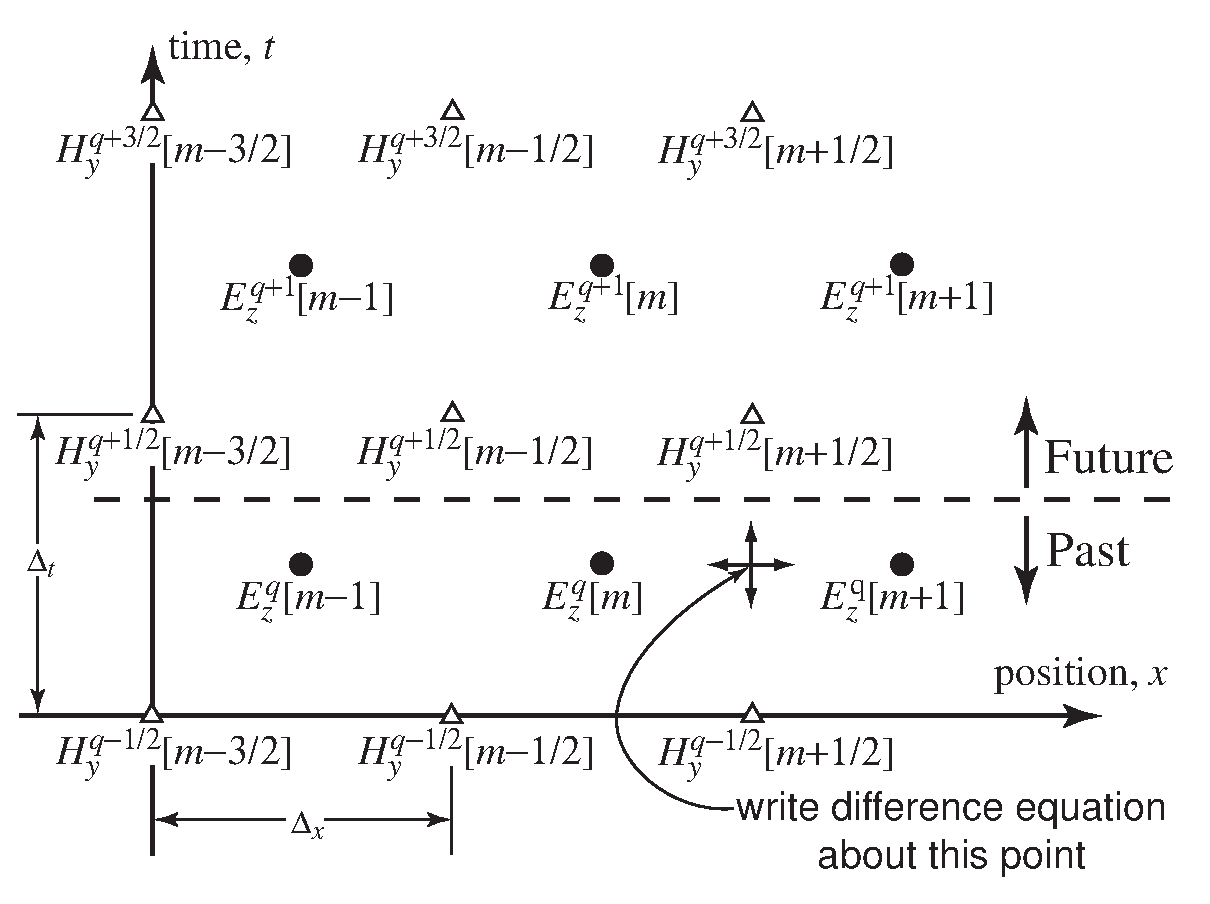
\epsfig{width=4.6in,file=Figures/Fdtd-intro/space-time-fdtd-update-new.eps}
  \end{center}
  \caption{The arrangement of electric- and magnetic-field nodes in
  space and time.  The electric-field nodes are shown as circles and
  the magnetic-field nodes as triangles.  The indicated point is where the
  difference equation is expanded to obtain an update equation for
  $H_y$.}
  \label{fig:spaceTime}
\end{figure}
The electric-field nodes are shown as circles and the magnetic-field
nodes as triangles.  Assume that all the fields below the dashed line
are known---they are considered to be in the past---while the fields
above the dashed line are future fields and hence unknown.  The FDTD
algorithm provides a way to obtain the future fields from the past
fields.

As indicated in Fig.\ \ref{fig:spaceTime}, consider Faraday's
law at the space-time point $((m+1/2)\Delx,q\Delt)$
\begin{equation}
  \left.\mu
  \frac{\partial H_y}{\partial t}\right|_{(m+1/2)\Delx,q\Delt}
  =
  \left.\frac{\partial E_z}{\partial x}\right|_{(m+1/2)\Delx,q\Delt}.
  \label{eq:faradayDiscrete}
\end{equation}
The temporal derivative is replaced by a finite difference involving
$\fdtdh{H_y}{m+\half}{q+\half}$ and $\fdtdh{H_y}{m+\half}{q-\half}$
(i.e., the magnetic field at a fixed location but two different times)
while the spatial derivative is replaced by a finite difference
involving $\fdtd{E_z}{m+1}{q}$ and $\fdtd{E_z}{m}{q}$ (i.e., the
electric field at two different locations but one time).  This yields
\begin{equation}
  \mu\frac{\fdtdh{H_y}{m+\half}{q+\half} -
           \fdtdh{H_y}{m+\half}{q-\half}}{\Delt} = 
  \frac{\fdtd{E_z}{m+1}{q} - \fdtd{E_z}{m}{q}}{\Delx}.
  \label{eq:faradayFdtd1D}
\end{equation}
Solving this for $\fdtdh{H_y}{m+\half}{q+\half}$ yields
\index{update equation!one-dimensional|(}
\begin{equation}
  \fdtdh{H_y}{m+\half}{q+\half} = \fdtdh{H_y}{m+\half}{q-\half} +
  \frac{\Delt}{\mu\Delx}
  \left(\fdtd{E_z}{m+1}{q} - \fdtd{E_z}{m}{q}\right).
  \label{eq:updateHy}
\end{equation}
This is known as an update equation, specifically the update equation
for the $H_y$ field.  It is a generic equation which can be applied to
any magnetic-field node.  It shows that the future value of $H_y$
depends on only its previous value and the neighboring electric
fields.  After applying \refeq{eq:updateHy} to all the magnetic-field
nodes, the dividing line between future and past values has advanced a
half time-step.  The space-time grid thus appears as shown in Fig.\
\ref{fig:spaceTimeUpdate} which is identical to Fig.\
\ref{fig:spaceTime} except for the advancement of the past/future
dividing line.

Now consider Ampere's law \refeq{eq:ampereScalar} applied at the
space-time point $(m\Delx,(q+1/2)\Delt)$ which is indicated in Fig.\
\ref{fig:spaceTimeUpdate}:
\begin{figure}
  \begin{center}
  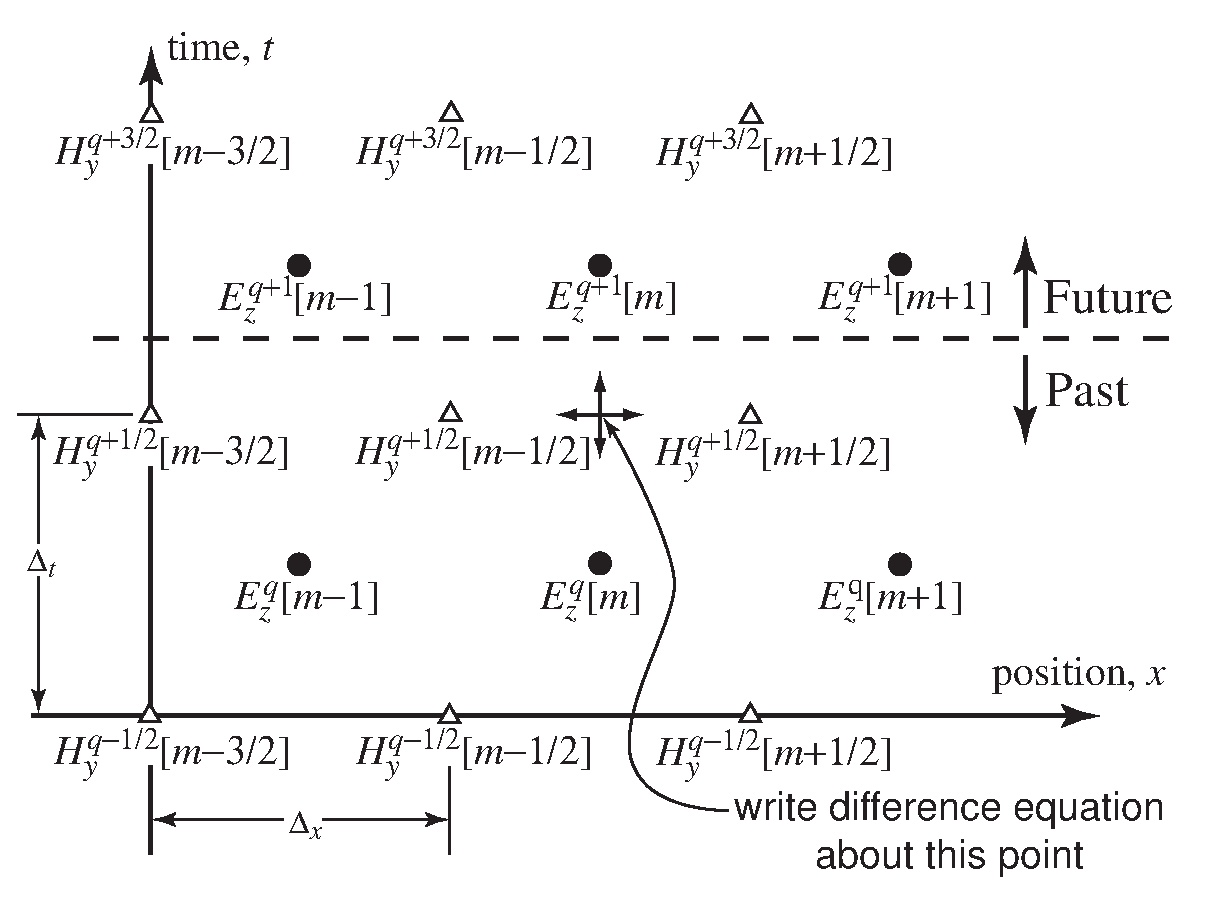
\epsfig{width=4.6in,file=Figures/Fdtd-intro/space-time-fdtd-new.eps}
  \end{center}
  \caption{Space-time after updating the magnetic field.  The dividing
  line between future and past values has moved forward a half
  temporal step.  The indicated point is where the difference equation
  is written to obtain an update equation for $E_z$.}
  \label{fig:spaceTimeUpdate}
\end{figure}
\begin{equation}
  \left.\epsilon
  \frac{\partial E_z}{\partial t}\right|_{m\Delx,(q+1/2)\Delt}
  =
  \left.\frac{\partial H_y}{\partial x}\right|_{m\Delx,(q+1/2)\Delt}.
\end{equation}
Replacing the temporal derivative on the left with a finite
difference involving $\fdtd{E_z}{m}{q+1}$ and $\fdtd{E_z}{m}{q}$
and replacing the spatial derivative on the right with a finite
difference involving $\fdtdh{H_y}{m+\half}{q+\half}$ and
$\fdtdh{H_y}{m-\half}{q+\half}$ yields
\begin{equation}
  \epsilon\frac{\fdtd{E_z}{m}{q+1} - \fdtd{E_z}{m}{q}}{\Delt} = 
  \frac{\fdtdh{H_y}{m+\half}{q+\half} - \fdtdh{H_y}{m-\half}{q+\half}}{\Delx}.
  \label{eq:ampereFdtd1D}
\end{equation}
Solving for $\fdtd{E_z}{m}{q+1}$ yields
\begin{equation}
  \fdtd{E_z}{m}{q+1} = \fdtd{E_z}{m}{q} + 
  \frac{\Delt}{\epsilon\Delx}
   \left(\fdtdh{H_y}{m+\half}{q+\half} - \fdtdh{H_y}{m-\half}{q+\half}\right).
  \label{eq:updateEz}
\end{equation}
Equation \refeq{eq:updateEz} is the update equation for the $E_z$
field.  The indices in this equation are generic so that the same
equation holds for every $E_z$ node.  Similar to the update equation for
the magnetic field, here we see that the future value of $E_z$ depends
on only its past value and the value of the neighboring magnetic
fields.
\index{update equation!one-dimensional|)}

After applying \refeq{eq:updateEz} to every electric-field node in the
grid, the dividing line between what is known and what is unknown
moves forward another one-half temporal step.  One is essentially back
to the situation depicted in Fig.\ \ref{fig:spaceTime}---the future
fields closest to the dividing line between the future and past are
magnetics fields.  They would be updated again, then the electric
fields would be updated, and so on.

It is often convenient to represent the update coefficients
$\Delt/\epsilon\Delx$ and $\Delt/\mu\Delx$ in terms of the ratio of
how far energy can propagate in a single temporal step to the spatial
step.  The maximum speed electromagnetic energy can travel is the
speed of light in free space $c=1/\sqrt{\epsilon_0\mu_0}$ and hence
the maximum distance energy can travel in one time step is $c\Delt$
(in all the remaining discussions the symbol $c$ will be reserved for
the speed of light in free space).  The ratio $c\Delt/\Delx$ is often
called the Courant number \index{Courant number!definition} which we
label $S_c$.  It plays an important role in determining the stability
of a simulation (hence the use of $S$) and will be considered further
later.  Letting $\mu=\mu_r\mu_0$ and $\epsilon=\epsilon_r\epsilon_0$,
the coefficients in \refeq{eq:updateEz} and \refeq{eq:updateHy} can be
written
\begin{eqnarray}
  \frac{1}{\epsilon} \frac{\Delt}{\Delx} \!&=&\!
    \frac{1}{\epsilon_r\epsilon_0}
    \frac{\sqrt{\epsilon_0\mu_0}}{\sqrt{\epsilon_0\mu_0}}
    \frac{\Delt}{\Delx} = 
    \frac{\sqrt{\epsilon_0\mu_0}}{\epsilon_r\epsilon_0}
    \frac{c\Delt}{\Delx} = 
    \frac{1}{\epsilon_r}
    \sqrt{\frac{\mu_0}{\epsilon_0}}
    \frac{c\Delt}{\Delx} = 
    \frac{\eta_0}{\epsilon_r}
    \frac{c\Delt}{\Delx} =
    \frac{\eta_0}{\epsilon_r} S_c
  \label{eq:coefEz} \\
  \frac{1}{\mu} \frac{\Delt}{\Delx} \!&=&\!
    \frac{1}{\mu_r\mu_0}
    \frac{\sqrt{\epsilon_0\mu_0}}{\sqrt{\epsilon_0\mu_0}}
    \frac{\Delt}{\Delx} = 
    \frac{\sqrt{\epsilon_0\mu_0}}{\mu_r\mu_0}
    \frac{c\Delt}{\Delx} = 
    \frac{1}{\mu_r}
    \sqrt{\frac{\epsilon_0}{\mu_0}}
    \frac{c\Delt}{\Delx} = 
    \frac{1}{\mu_r\eta_0}
    \frac{c\Delt}{\Delx} =
    \frac{1}{\mu_r\eta_0} S_c
    \label{eq:coefHy}
\end{eqnarray}
where $\eta_0=\sqrt{\mu_0/\epsilon_0}$ is the characteristic impedance
of free space.

In FDTD simulations there are restrictions on how large a temporal
step can be.  If it is too large, the algorithm produces unstable
results (i.e., the numbers obtained are completely meaningless and
generally tend quickly to infinity).  At this stage we will not
consider a rigorous analysis of stability.  However, thinking about
the way fields propagate in an FDTD grid, it seems logical that energy
should not be able to propagate any further than one spatial step for
each temporal step, i.e., $c\Delt\le\Delx$.  This is because in the
FDTD algorithm each node only affects its nearest neighbors.  In one
complete cycle of updating the fields, the furthest a disturbance could
propagate is one spatial step.  It turns out that the optimum ratio
for the Courant number (in terms of minimizing numeric errors)
is also the maximum ratio.  Hence, for the one-dimensional simulations
considered initially, we will use
\begin{equation}
  S_c = \frac{c\Delt}{\Delx} = 1.
\end{equation}

When first obtaining the update equations for the FDTD algorithm, it
is helpful to think in terms of space-time.  However, treating time as
an additional dimension can be awkward.  Thus, in most situations it
is more convenient to think in terms of a single spatial dimension
where the electric and magnetic fields are offset a half spatial step
from each other.  This is depicted in Fig.\
\ref{fig:fdtdOneD}.  The temporal offset between the electric and
magnetic field is always understood whether explicitly shown or not.
\begin{figure}
  \begin{center}
  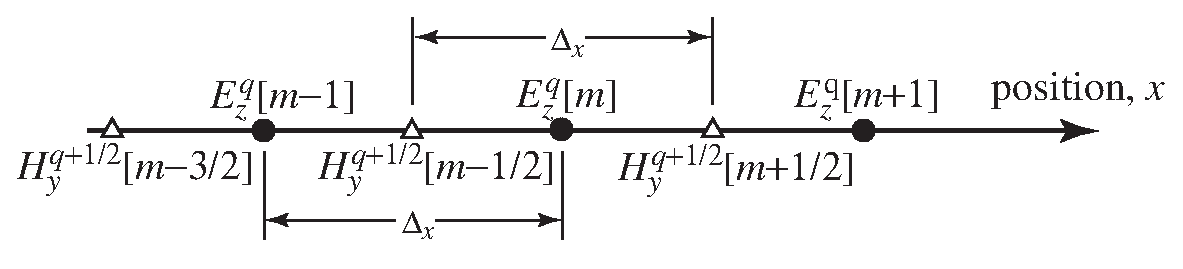
\epsfig{width=5.0in,file=Figures/Fdtd-intro/space-fdtd-1d.eps}
  \end{center}
  \caption{A one-dimensional FDTD space showing the spatial offset
  between the magnetic and electric fields.}
  \label{fig:fdtdOneD}
\end{figure}


\section{Computer Implementation of a One-Dimensional\\ FDTD Simulation}

Our goal now is to translate the update equations \refeq{eq:updateHy}
and \refeq{eq:updateEz} into a usable computer program.  The first
step is to discard, at least to a certain extent, the
superscripts---time is a global parameter and will be recorded in a
single integer variable.  Time is not something about which each node
needs to be concerned.

Next, keep in mind that in most computer languages the equal sign is
used as ``the assignment operator.''  In C, the following is a
perfectly valid statement
\begin{verbatim}
  a = a+b;
\end{verbatim}
In the usual mathematical sense, this statement is only true if $b$
were zero.  However, to a computer this statement means take the value
of $b$, add it to the old value of $a$, and place the result back in
the variable $a$.  Essentially we are updating the value of $a$.  In C
this statement can be written more tersely as
\begin{verbatim}
  a += b;
\end{verbatim}

When writing a computer program to implement the FDTD algorithm, one
does not bother trying to construct a program that explicitly uses
offsets of one-half.  Nodes are stored in arrays and, as is standard
practice, individual array elements are specified with integer
indices.  Thus, the computer program (or, perhaps more correctly, the
{\em author} of the computer program) implicitly incorporates the fact
that electric and magnetic fields are offset while using only integer
indices to specify location.  As you will see, spatial location and
the array index will be virtually synonymous.

For example, assume two arrays, {\tt ez} and {\tt hy}, are
declared which will contain the $E_z$ and $H_y$ fields at 200 nodes
\begin{verbatim}
  double ez[200], hy[200], imp0=377.0;
\end{verbatim}
The variable {\tt imp0} is the characteristic impedance of free space
and will be used in the following discussion (it is initialized to a
value of $377.0$ in this declaration).  One should think of the
elements in the {\tt ez} and {\tt hy} arrays as being offset from
each other by a half spatial step even though the array values will be
accessed using an integer index.  

It is arbitrary whether one initially wishes to think of an {\tt ez}
array element as existing to the right or the left of an {\tt hy}
element with the same index (we assume ``left'' corresponds to
descreasing values of $x$ while ``right'' corresponds to increasing
values).  Here we will assume {\tt ez} nodes are to the left of {\tt
  hy} nodes with the same index.  This is illustrated in Fig.\
\ref{fig:oneDArrays} where {\tt ez[0]} is to the left of {\tt hy[0]},
{\tt ez[1]} is to the left of {\tt hy[1]}, and so on.  In general,
when a Courier font is used, e.g., {\tt hy[m]}, we are considering an
array and any offsets of one-half associated with that array are
implicitly understood.  When Times-Italic font is use, e.g.,
$\fdtdh{H_y}{m+\half}{q+\half}$ we are discussing the field itself and
offsets will be given explicitly.
\begin{figure}
  \begin{center}
  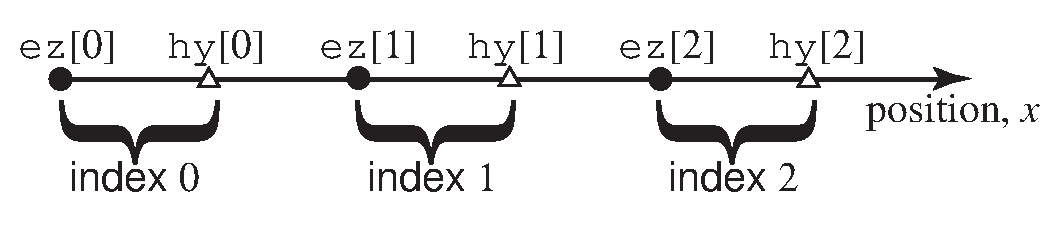
\epsfig{width=5.0in,file=Figures/Fdtd-intro/fdtd-1d-computer.eps}
  \end{center}
  \caption{A one-dimensional FDTD space showing the assumed spatial
  arrangement of the electric- and magnetic-field nodes in the arrays
  {\tt ez} and {\tt hy}.  Note that an electric-field node is assumed
  to exist to the left of the magnetic-field node with the same
  index.}  \label{fig:oneDArrays}
\end{figure}

Assuming a Courant number of unity ($S_c=1$), the node {\tt hy[1]}
could be updated with a statement such as
\begin{verbatim}
  hy[1] = hy[1] + (ez[2] - ez[1]) / imp0;
\end{verbatim}
In general, any magnetic-field node can be updated with
\begin{verbatim}
  hy[m] = hy[m] + (ez[m + 1] - ez[m]) / imp0;
\end{verbatim}
For the electric-field nodes, the update equation can be written
\begin{verbatim}
  ez[m] = ez[m] + (hy[m] - hy[m - 1]) * imp0;
\end{verbatim}
These two update equations, placed in appropriate loops, are the
engines that drive an FDTD simulation.  However, there are a few
obvious pieces missing from the puzzle before a useful simulation can
be performed.  These missing pieces include
\begin{enumerate}
\item Nodes at the end of the physical space do not have neighboring
  nodes to one side.  For example, there is no {\tt hy[-1]} node for
  the {\tt ez[0]} node to use in its update equation.  Similarly, if
  the arrays are declared with 200 element, there is no {\tt ez[200]}
  available for {\tt hy[199]} to use in its update equation (recall
  that the index of the last element in a C array is one less than the
  total number of elements---the array index represents the offset
  from the first element of the array).  Therefore a standard update
  equation cannot be used at these nodes.

\item Only a constant impedance is used so only a homogeneous medium
  can be modeled (in this case free space).

\item As of yet there is no energy present in the field.  If the
  fields are initially zero, they will remain zero forever.
\end{enumerate}

The first issue can be addressed using absorbing boundary conditions
(ABC's).  There are numerous implementations one can use.  In later
material we will be consider only a few of the more popular
techniques.

The second restriction can be removed by allowing the permittivity and
permeability to change from node to node.  However, in the interest of
simplicity, we will continue to use a constant impedance for a little
while longer.

The third problem can be overcome by initializing the fields to a
non-zero state.  However, this is cumbersome and typically not a good
approach.  Better solutions are to introduce energy via either a
hardwired source, an additive source, or a total-field/scattered-field
(TFSF) boundary.  We will consider implementation of each of these
approaches.

\section{Bare-Bones Simulation \label{sec:bareBones}}

Let us consider a simulation of a wave propagating in free space where 
there are 200 electric- and magnetic-field nodes.  The code is shown
in Program \ref{pro:1DbareBones}.
\begin{program}
{\tt 1DbareBones.c}: \index{1DbareBones.c@{\tt 1DbareBones.c}}
Bare-bones one-dimensional simulation with a hard
source. \label{pro:1DbareBones}
\codemiddle
\begin{lstlisting}
/* Bare-bones 1D FDTD simulation with a hard source. */

#include <stdio.h>
#include <math.h>

#define SIZE 200

int main()
{
  double ez[SIZE] = {0.}, hy[SIZE] = {0.}, imp0 = 377.0; /*@ \label{bareBonesA} @*/
  int qTime, maxTime = 250, mm;              /*@ \label{bareBonesB} @*/

  /* do time stepping */
  for (qTime = 0; qTime < maxTime; qTime++) {  /*@ \label{bareBonesC} @*/

    /* update magnetic field */
    for (mm = 0; mm < SIZE - 1; mm++)            /*@ \label{bareBonesD} @*/
      hy[mm] = hy[mm] + (ez[mm + 1] - ez[mm]) / imp0;

    /* update electric field */
    for (mm = 1; mm < SIZE; mm++)              /*@ \label{bareBonesE} @*/
      ez[mm] = ez[mm] + (hy[mm] - hy[mm - 1]) * imp0;

    /* hardwire a source node */
    ez[0] = exp(-(qTime - 30.) * (qTime - 30.) / 100.); /*@ \label{bareBonesF} @*/

    printf("%g\n", ez[50]); /*@ \label{bareBonesG} @*/
  } /* end of time-stepping */

  return 0;
}
\end{lstlisting}
\end{program}
In the declaration of the field arrays in line \ref{bareBonesA},
``{\tt=\{0.\}}'' has been added to ensure that these arrays are
initialized to zero.  (For larger arrays this is not an efficient
approach for initializing the arrays and we will address this fact
later.)  The variable {\tt qTime} is an integer counter that serves as
the temporal index or time step.  The total number of time steps in
the simulation is dictated by the variable {\tt maxTime} which is set
to $250$ in line \ref{bareBonesB} ($250$ was chosen arbitrarily---it
can be any value desired).

Time-stepping is accomplished with the for-loop that begins on line
\ref{bareBonesC}.  Embedded within this time-stepping loop are two
additional (spatial) loops---one to update the magnetic field and the
other to update the electric field.  The magnetic-field update loop
starting on line \ref{bareBonesD} excludes the last magnetic-field
node in the array, {\tt hy[199]}, since this node lacks one
neighboring electric field.  For now we will leave this node zero.
The electric-field update loop in line \ref{bareBonesE} starts with a
spatial index {\tt m} of $1$, i.e., it does not include {\tt ez[0]}
which is the first $E_z$ node in the grid.  The value of {\tt ez[0]}
is dictated by line \ref{bareBonesF} which is a Gaussian function that
will have a maximum value of unity when the time counter {\tt qTime}
is $30$.  The first time through the loop, when {\tt qTime} is zero,
{\tt ez[0]} will be set to $\exp(-9)\approx 1.2341\times 10^{-4}$
which is small relative to the maximum value of the source.  Line
\ref{bareBonesG} prints the value of {\tt ez[50]} to the screen, once
for each time step.  A plot of the output generated by this program is
shown in Fig.\
\ref{fig:bareBones}.
\begin{figure}
  \begin{center}
  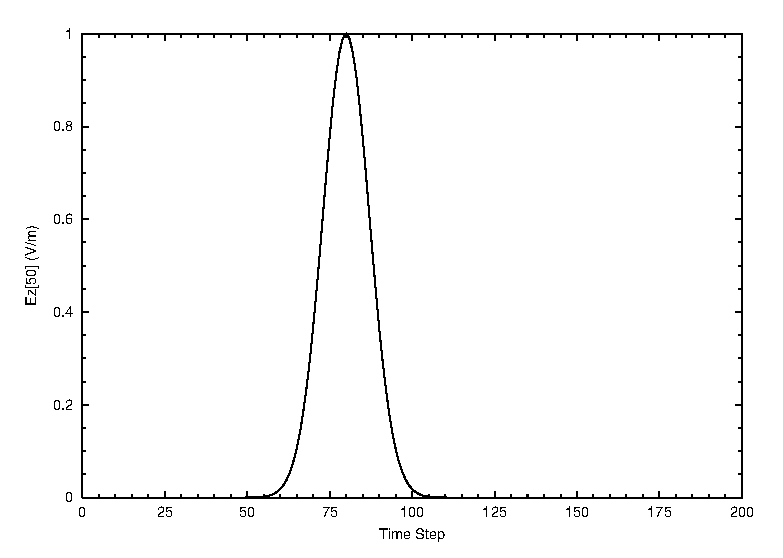
\epsfig{width=4.6in,file=Code/Fdtd-intro/bare-bones-output200.eps}
  \end{center}
  \caption{Output generated by Program \ref{pro:1DbareBones}.}
  \label{fig:bareBones} 
\end{figure}

Note that the output is a Gaussian.  The excitation is introduced at
{\tt ez[0]} but the field is recorded at {\tt ez[50]}.  Because
$c\Delt=\Delx$ in this simulation (i.e., the Courant number is unity),
the field moves one spatial step for every time step.  The separation
between the source point and the observation point results in the
observed signal being delayed by $50$ time steps from what it was at
the source.  The source function has a peak at $30$ time steps but, as
can be seen from Fig.\ \ref{fig:bareBones}, the field at the
observation point is maximum at time step $80$.

Consider a slight modification to Program \ref{pro:1DbareBones} where
the simulation is run for $1000$ time steps instead of $250$ (i.e.,
{\tt maxTime} is set to $1000$ in line \ref{bareBonesB} instead of
$250$).  The output obtained in this case is shown in Fig.\
\ref{fig:bareBonesLong}.
\begin{figure}
  \begin{center}
  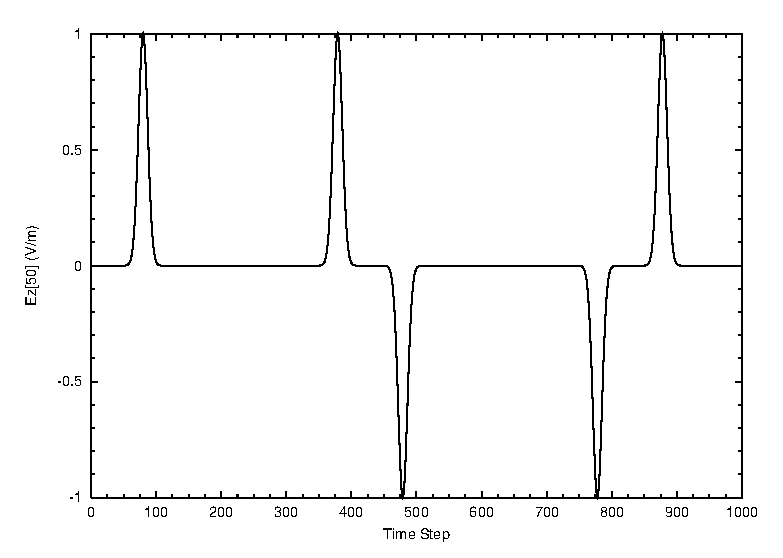
\epsfig{width=4.6in,file=Code/Fdtd-intro/bare-bones-output1000.eps}
  \end{center}
  \caption{Output generated by Program \ref{pro:1DbareBones} but with
  {\tt maxTime} set to $1000$.}
  \label{fig:bareBonesLong} 
\end{figure}
Why are there multiple peaks here and why are they both positive and
negative?

The last magnetic-field node in the grid is initially zero and remains
zero throughout the simulation.  When the field encounters this node
it essentially see a perfect magnetic conductor (PMC).  To satisfy the
boundary condition at this node, i.e., that the total magnetic field
go to zero, a reflected wave is created which reverses the sign of the
magnetic field but preserves the sign of the electric field.  This
phenomenon is considered in more detail in the next section.  The
second peak in Fig.\ \ref{fig:bareBonesLong} is this reflected wave.
The reflected wave continues to travel in the negative direction until
it encounters the first electric-field node {\tt ez[0]}.  This node
has its value set by the source function and is oblivious to what is
happening in the interior of the grid.  In this particular case, by
the time the reflected field reaches the left end of the grid, the
source function has essentially gone to zero and nothing is going to
change that.  Thus the node {\tt ez[0]} behaves like a perfect
electric conductor (PEC).  To satisfy the boundary conditions at this
node, the wave is again reflected, but this time the electric field
changes sign while the sign of the magnetic field is preserved.  In
this way the field which was introduced into the grid continues to
bounce back and forth until the simulation is terminated.  The
simulation is of a resonator with one PMC wall and one PEC wall.
(Note that the boundary condition at {\tt ez[0]} is the same whether
or not the source function has gone to zero.  Any incoming field
cannot change the value at {\tt ez[0]} and hence a reflected wave must
be generated which has equal magnitude but opposite sign from the
incoming field.)

%%%%%%%%%%%%%%%%%%%%%%%%%%%%%%%%%%%%%%%%%%%%%%%%%%%%%%%%%%%%%%%%%%%%%%%%%
\section{PMC Boundary in One Dimension \label{sec:pmcBoundary}} 

In Program \ref{pro:1DbareBones} one side of the grid (the ``right
side'') is terminated by a magnetic field which is always zero.  It
was observed that this node acts as a perfect magnetic conductor (PMC)
which produces a reflected wave where the electric field is not
inverted while the magnetic field is inverted.  To understand fully
why this is the case, let us consider the right side of a
one-dimensional domain where $200$ electric- and magnetic-field nodes
are used to model free space.  Assume the Courant number is unity and
the impedance of free space is $377$.  The last node in the grid is
{\tt hy[199]} and it will always remain zero.  The other nodes in the
grid are updated using, in C notation:
\begin{eqnarray}
  \mbox{\tt\ \ \ \ ez[m] = ez[m] + (hy[m] - hy[m - 1]) * 377;} \label{eq:ezUpdateC}\\
  \mbox{\tt\ \ \ \ hy[m] = hy[m] + (ez[m + 1] - ez[m]) / 377;} \label{eq:hyUpdateC}
\end{eqnarray}
Assume that a Dirac delta pulse, i.e., a unit amplitude pulse existing
at a single electric-field node in space-time, is nearing the end of
the grid.  Table \ref{tab:pmcBoundary} shows the fields at progressive
time-steps starting at a time $q$ when the pulse has reached node {\tt
ez[198]}.

\renewcommand{\multirowsetup}{\centering}
\newlength{\LL}\settowidth{\LL}{time}
\begin{table}
\begin{center}
\begin{tabular}{cl|cccccc}
\multirow{12}{\LL}{time\\step}& & \multicolumn{6}{c}{node} \\
&
& {\tt ez[197]} &{\tt hy[197]} &{\tt ez[198]}&
  {\tt hy[198]} &{\tt ez[199]} &{\tt hy[199]}\\ \hline
& $q-1/2$&       &$-1/377$ &     &$0$      &       &$0$\\
& $q$    &  $0$  &         &$1$  &         &$0$    &\\ \cline{2-8}
& $q+1/2$&       &$0$      &     &$-1/377$ &       &$0$\\
& $q+1$  &  $0$  &         &$0$  &         &$1$    &\\ \cline{2-8}
& $q+3/2$&       &$0$      &     &$0$      &       &$0$\\
& $q+2$  &  $0$  &         &$0$  &         &$1$    &\\ \cline{2-8}
& $q+5/2$&       &$0$      &     &$1/377$  &       &$0$\\
& $q+3$  &  $0$  &         &$1$  &         &$0$    &\\ \cline{2-8}
& $q+5/2$&       &$1/377$  &     &$0$      &       &$0$ \\
& $q+4$  &  $1$  &         &$0$  &         &$0$    &
\end{tabular}
\end{center}
\caption{Electric- and magnetic-field nodes at the ``end'' of arrays
 which have 200 elements, i.e., the last node is {\tt hy[199]} which is
 always set to zero.  A pulse of unit amplitude is propagating to the
 right and has arrived at {\tt ez[198]} at time-step $q$.  Time is
 advancing as one reads down the columns.}
\label{tab:pmcBoundary}
\end{table}

At time $q$ node {\tt ez[198]} is unity while {\tt hy[197]} was set to
$-1/377$ at the previous update of the magnetic fields.  When the
magnetic fields are updated at time $q+1/2$ the update equation
\refeq{eq:hyUpdateC} dictates that {\tt hy[197]} be set to zero (the
``old'' value of the magnetic field cancels the contribution from the
electric field).  Meanwhile, {\tt hy[198]} becomes $-1/377$.  All
other magnetic-field nodes will be zero.

Updating the electric field at time-step $q+1$ results in {\tt
ez[198]} being set to zero while {\tt ez[199]} is set to one---the
pulse advances one spatial step to the right.  If the normal update
equation could be used at node {\tt hy[199]}, at time $q+3/2$ it would
be set to $-1/377$.  However, because there is no neighboring electric
field to the right of {\tt hy[199]}, the update equation cannot be
used and, lacking an alternative way of calculating its value, {\tt
hy[199]} is left as zero.  Thus at time $q+3/2$ {\em all} the
magnetic-field nodes in the grid are zero.

When the electric field is updated at time $q+2$ essentially nothing
happens.  The electric fields are updated from their old values and
the difference of surrounding magnetic fields.  However all magnetic
fields are zero.  Thus the new electric field is the same as the old
electric field.

At time $q+5/2$ the unit pulse which exists at {\tt ez[199]} causes
{\tt hy[198]} to become $1/377$ which is the negative of what it was two
times steps ago.  From this time forward, the pulse propagates back to
the left with the electric field maintaining unit amplitude.

This discussion is for a single pulse, but any incident field could be
treated as a string of pulses and then one would merely have to
superimpose their values.  This dicussion further supposes the Courant
number is unity.  When the Courant number is not unity the termination
of the grid still behaves as a PMC wall, but the pulse will not
propagate without distortion (it suffers dispersion because of the
properties of the grid itself as will be discussed in more detail in
Sec.\ \ref{sec:gridDispersion}).

If the grid were terminated on an electric-field node which was
always set to zero, that node would behave as a perfect electric
conductor.  In that case the reflected electric field would have the
opposite sign from the incident field while the magnetic field would
preserve its sign.  This is what happens to any field incident on the
left side of the grid in Program \ref{pro:1DbareBones}.

\section{Snapshots of the Field}

In Program \ref{pro:1DbareBones} the field at a single point is
recorded to a file.  Alternatively, it is often useful to view the
fields over the entire computational domain at a single instant of
time, i.e., take a ``snapshot'' that shows the field throughout space.
Here we describe one way in which this can be conveniently implemented
in C.

The approach adopted here will open a separate file for each snapshot.
Each file will have a common base name, then a dot, and then a
sequence number which will be called the frame number.  So, for
example, the files might be called {\tt sim.0}, {\tt sim.1}, {\tt
sim.2}, and so on.  To accomplish this, the fragments shown in
Fragments \ref{frag:snapshot} and \ref{frag:snapshotI} would be added to a
program (such as Program \ref{pro:1DbareBones}).
\begin{fragment}
  Declaration of variables associated with taking snapshots.  The base
  name is stored in the character array {\tt basename} and the
  complete file name for each frame is stored in {\tt filename}.  Here
  the base name is initialized to {\tt sim} but, if desired, the user
  could be prompted for the base name.  The integer {\tt frame} is the
  frame number for each snapshot and is initialized to
  zero. \label{frag:snapshot}
  \codemiddle
\begin{lstlisting}
  char basename[80] = "sim", filename[100];
  int frame = 0;
  FILE *snapshot;
\end{lstlisting}
\end{fragment}
\begin{fragment}
  Code to generate the snapshots.  This would be placed inside the
  time-stepping loop.  The initial if statement ensures the electric
  field is recorded every tenth time-step.\label{frag:snapshotI}
  \codemiddle
\begin{lstlisting}
    /* write snapshot if time-step is a multiple of 10 */
    if (qTime % 10 == 0) {                       /*@ \label{fragSnapA} @*/
      /* construct complete file name and increment frame counter */
      sprintf(filename, "%s.%d", basename, frame++); /*@ \label{fragSnapB} @*/

      /* open file */
      snapshot = fopen(filename, "w");  /*@ \label{fragSnapC} @*/

      /* write data to file */
      for (mm = 0; mm < SIZE; mm++)     /*@ \label{fragSnapD} @*/
        fprintf(snapshot, "%g\n", ez[mm]);

      /* close file */
      fclose(snapshot);                 /*@ \label{fragSnapE} @*/
    }
\end{lstlisting}
\end{fragment}

In Fragment \ref{frag:snapshot} the base name is initialized to {\tt
  sim} but the user could be prompted for this.  The integer variable
{\tt frame} is the frame (or snapshot) counter that will be
incremented each time a snapshot is taken.  It is initialized to zero.
The file pointer {\tt snapshot} is used for the output files.

The code shown in Fragment \ref{frag:snapshotI} would be placed inside
the time-stepping loop of Program \ref{pro:1DbareBones}.  Line
\ref{fragSnapA} checks, using the modulo operator ({\tt \%}) if the
time step is a multiple of $10$.  ($10$ was chosen somewhat
arbitrarily.  If snapshots were desired more frequently, a smaller
value would be used.  If snapshots were desired less frequently, a
larger value would be used.)  If the time step is a multiple of $10$,
the complete output-file name is constructed in line \ref{fragSnapB}
by writing the file name to the string variable {\tt filename}.
(Since zero is a multiple of $10$, the first snapshot that is taken
corresponds to the fields at time zero.  This data would be written to
the file {\tt sim.0}.  Note that in Line \ref{fragSnapB} the frame
number is incremented each time a file name is created.  The file is
opened in line \ref{fragSnapC} and the data is written using the loop
starting in line \ref{fragSnapD}.  Finally, the file is closed in line
\ref{fragSnapE}.

Fig.\ \ref{fig:snapshots} shows the snapshots of the field at time
steps $20$, $30$, and $40$ using essentially the same code as Program
\ref{pro:1DbareBones}---the only difference being the addition of the
code to take the snapshots.  The corresponding files are {\tt sim.2},
{\tt sim.3}, and {\tt sim.4}.  In these snapshots the field can be
seen entering the computational domain from the left and propagating
to the right.

\begin{figure}
  \begin{center}
  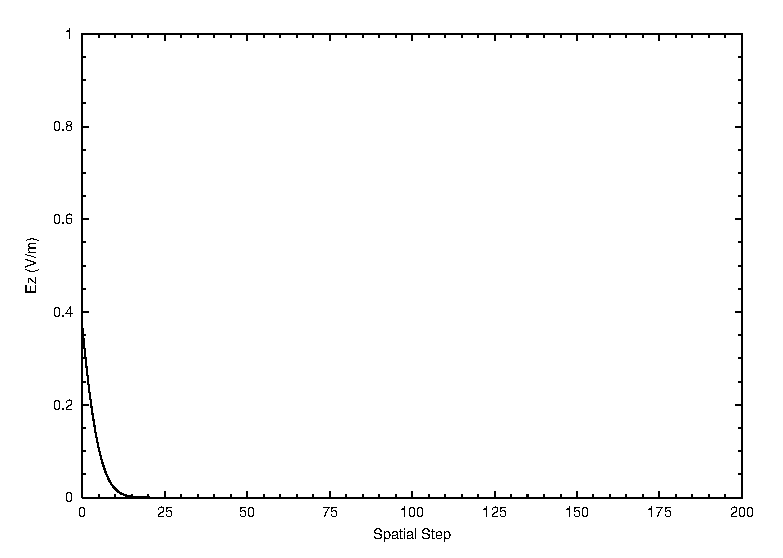
\epsfig{width=3.5in,file=Code/Fdtd-intro/snapshot1.eps}
  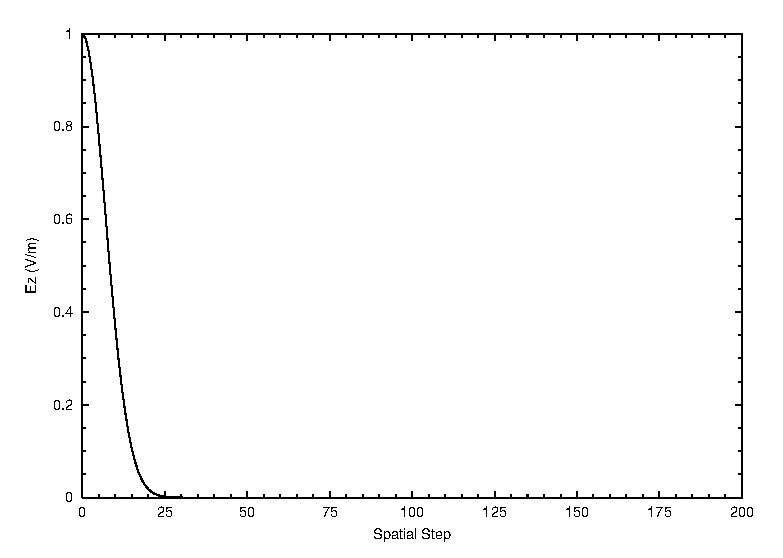
\epsfig{width=3.5in,file=Code/Fdtd-intro/snapshot2.eps}
  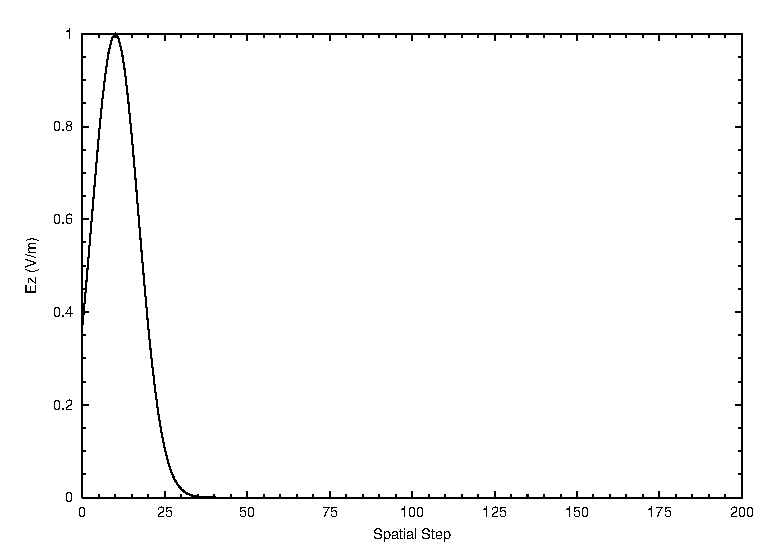
\epsfig{width=3.5in,file=Code/Fdtd-intro/snapshot3.eps}
\end{center} \caption{Snapshots taken at time-steps $20$, $30$, and
  $40$ of the $E_z$ field generated by Program \ref{pro:1DbareBones}.
  The field is seen to be propagating away from the hardwired source
  at the left end of the grid.}  \label{fig:snapshots}
\end{figure}

\section{Additive Source \label{sec:additive}}

Hardwiring the source, as was done in Program \ref{pro:1DbareBones},
has the severe shortcoming that no energy can pass through the source
node.  This problem can be rectified by using an additive source.
Consider Ampere's law with the current density term:
\begin{equation}
  \nabla\times\Hvec = \Jvec + 
                      \epsilon\frac{\partial \Evec}{\partial t}.
  \label{eq:ampereWithCurrent}
\end{equation}
The current density $\Jvec$ can represent both the conduction current
due to flow of charge in a material under the influence of the
electric field, i.e., current given by $\sigma\Evec$, as well as the
current associated with any source, i.e., an ``impressed current.''
At this point we are just interested in the source aspect of $\Jvec$
and will return to the issue of finite conductivity in Sec.\
\ref{sec:loss} and Sec.\ \ref{sec:conductivity}.  Rearranging
\refeq{eq:ampereWithCurrent} slightly yields
\begin{equation}
  \frac{\partial \Evec}{\partial t} =
     \frac{1}{\epsilon} \nabla\times\Hvec - \frac{1}{\epsilon}\Jvec.
  \label{eq:ampereTweak}
\end{equation}
This equation gives the temporal derivative of the electric field in
terms of the spatial derivative of the magnetic field---which is as
before---and an additional term which can be thought of as the forcing
function for the system.  This current can be specified to be whatever
is desired.

To translate \refeq{eq:ampereTweak} into a form suitable for the FDTD
algorithm, the spatial derivatives are again expressed in terms of
finite differences and then one solves for the future fields in terms
of past fields.  Recall that for Ampere's law, the update equation for
$\fdtd{E_z}{m}{q}$ was obtained by applying finite differences at the
space-time point $(m\Delx,(q+1/2)\Delt)$.  Going through the exact
same procedure but adding the source term yields
\begin{equation}
  \fdtd{E_z}{m}{q+1} = \fdtd{E_z}{m}{q} + 
  \frac{\Delt}{\epsilon\Delx}
   \left(\fdtdh{H_y}{m+\half}{q+\half} - \fdtdh{H_y}{m-\half}{q+\half}\right)
  - \frac{\Delt}{\epsilon}\fdtd{J_z}{m}{q+\half}.
  \label{eq:updateEzSource}
\end{equation}
The source current could potentially be distributed over a number of
nodes, but for the sake of introducing energy to the grid, it suffices
to apply it to a single node.

In order to preserve the original update equation (which is sometimes
handy when writing loops), \refeq{eq:updateEzSource} can be separated
into two steps: first the usual update is applied and then the source
term is added.  For example:
\begin{eqnarray}
  \fdtd{E_z}{m}{q+1} &=& \fdtd{E_z}{m}{q} + \frac{\Delt}{\epsilon\Delx}
    \left(\fdtdh{H_y}{m+\half}{q+\half} - \fdtdh{H_y}{m-\half}{q+\half}\right) \\
  \fdtd{E_z}{m}{q+1} &=& \fdtd{E_z}{m}{q+1} -
    \frac{\Delt}{\epsilon}\fdtd{J_z}{m}{q+\half}. \label{eq:addCurrent1D}
\end{eqnarray}
In practice the source current might only exist at a single node in
the 1D grid (as will be the case in the examples to come).  Thus,
\refeq{eq:addCurrent1D} would be applied only at the node where the
source current is non-zero.

Generally the amplitude and the sign of the source function are not a
concern.  When calculating things such as the scattering cross-section
or the reflection coefficient, one always normalizes by the incident
field.  Therefore we do not need to specify explicitly the value of
$\Delt/\epsilon$ in \refeq{eq:addCurrent1D}---it suffices to merely
treat this coefficient as being contained in the source function
itself.

A program that implements an additive source and takes snapshots of
the electric field is shown in Program \ref{pro:1Dadditive}.  The
changes from Program \ref{pro:1DbareBones} are shown in bold.  The
source function is exactly the same as before except now, instead of
setting the value of {\tt ez[0]} to the value of this function, the
source function is added to {\tt ez[50]}.  The source is introduced in
line \ref{1DadditiveE} and the update equations are unchanged from
before.  (Note that in this chapter the programs will be somewhat
verbose, simplistic, and repetitive.  Once we are comfortable with the
FDTD algorithm we will pay more attention to better coding practices.)
\begin{program}
{\tt 1Dadditive.c}: \index{1Dadditive.c@{\tt 1Dadditive.c}}
One-dimensional FDTD program with an additive
source. \label{pro:1Dadditive} 
\codemiddle
\begin{lstlisting}
/* 1D FDTD simulation with an additive source. */

#include <stdio.h>
#include <math.h>

#define SIZE 200

int main()
{
  double ez[SIZE] = {0.}, hy[SIZE] = {0.}, imp0 = 377.0;
  int qTime, maxTime = 200, mm;
/*b*/
  char basename[80] = "sim", filename[100];
  int frame = 0;
  FILE *snapshot;
/*n*/
  /* do time stepping */
  for (qTime = 0; qTime < maxTime; qTime++) {
                                                  /*@ \label{1DadditiveA} @*/
    /* update magnetic field */                   /*@ \label{1DadditiveB} @*/
    for (mm = 0; mm < SIZE - 1; mm++)
      hy[mm] = hy[mm] + (ez[mm + 1] - ez[mm]) / imp0;
                                                  /*@ \label{1DadditiveC} @*/
    /* update electric field */                   /*@ \label{1DadditiveD} @*/
    for (mm = 1; mm < SIZE; mm++)
      ez[mm] = ez[mm] + (hy[mm] - hy[mm - 1]) * imp0;
/*b*/
    /* use additive source at node 50 */
    ez[50] += exp(-(qTime - 30.) * (qTime - 30.) / 100.); /*@ \label{1DadditiveE} @*/

    /* write snapshot if time a multiple of 10 */
    if (qTime % 10 == 0) {
      sprintf(filename, "%s.%d", basename, frame++);
      snapshot=fopen(filename, "w");
      for (mm = 0; mm < SIZE; mm++)
        fprintf(snapshot, "%g\n", ez[mm]);
      fclose(snapshot);
    }/*n*/
  } /* end of time-stepping */

  return 0;
}
\end{lstlisting}
\end{program}

Snapshots of $E_z$ taken at time-steps $20$, $30$, and $40$ are shown
in Fig.\ \ref{fig:additive}.  Note that the field originates from node
$50$ and that it propagates to either side of this node.  Also notice
that the peak amplitude is half of what it was when the source
function was implemented as a hardwired source.
\begin{figure}
  \begin{center}
  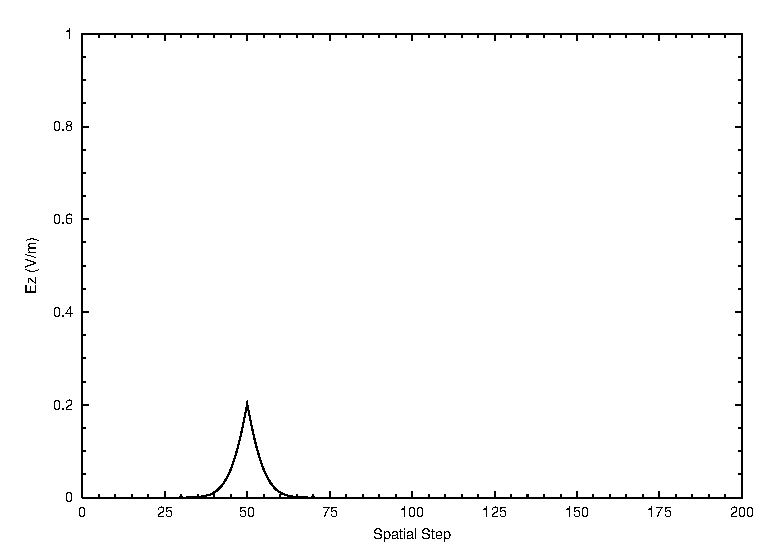
\epsfig{width=3.5in,file=Code/Fdtd-intro/additive1.eps}
  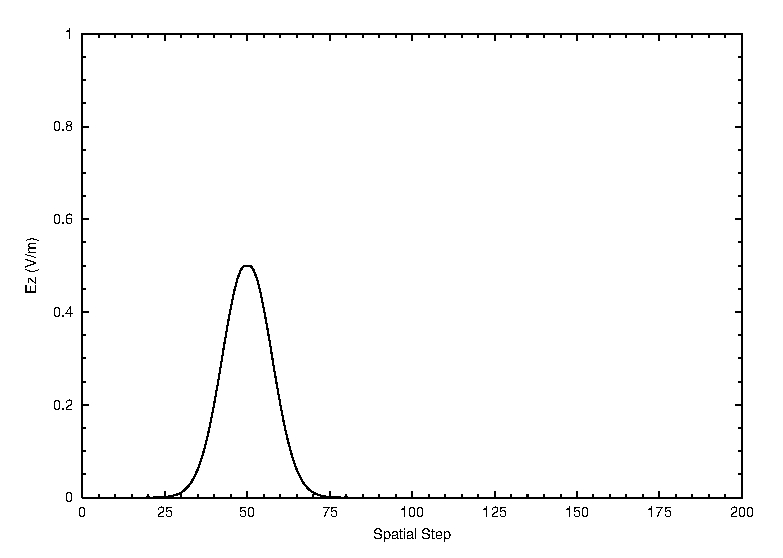
\epsfig{width=3.5in,file=Code/Fdtd-intro/additive2.eps}
  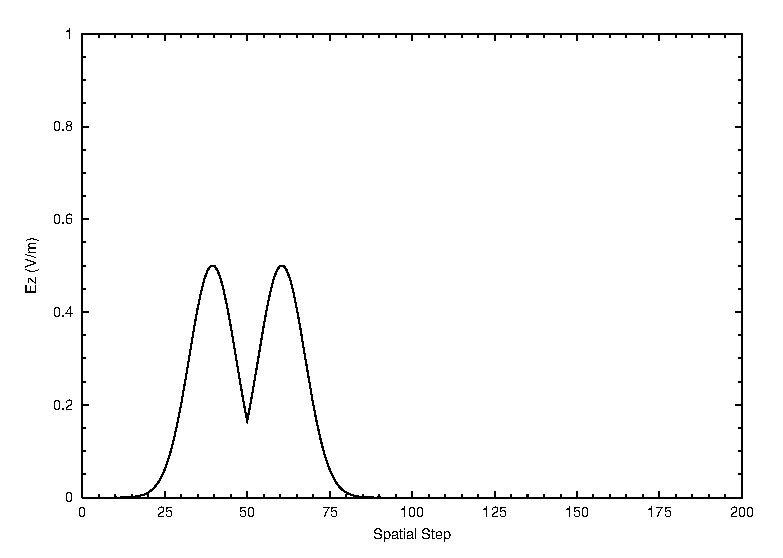
\epsfig{width=3.5in,file=Code/Fdtd-intro/additive3.eps}
  \end{center}
  \caption{Snapshots taken at time-steps $20$, $30$, and $40$ of the
    $E_z$ field generated by Program \ref{pro:1Dadditive}.  An
    additive source is applied to node $50$ and the field is seen to
    propagate away from it to either side.}
  \label{fig:additive} 
\end{figure}

As something of an aside, in Program \ref{pro:1Dadditive} note that
the code that takes a snapshot of the electric field was placed in the
time-stepping but after the update equation.  Thus one might ask: do
the contents of snapshot file {\tt sim.0} contain the fields at time
zero or at time one?  And, do the other snapshots correspond to times
that multiples of $10$ or do the correspond to one plus a multiple of
$10$?  In nearly all practical cases it won't matter.  The precise
location of $t=0$ is rather aribtrary.  So, when looking at the
snapshots it is usually sufficient to know that the sequence of
snapshots start ``at the beginning of the simulation'' and then are
taken every $10$ time steps.  However, if one wants to be more precise
about this, absolute time is usually dictated by the source function.
Now, think in terms of the hard-source implementation rather than the
additive source.  We have implemented a Gaussian source that has a
peak amplitude at time-step $30$.  The way the code is written here,
with the source being applied after the update equation and then the
snapshot being taken last, we would see the peak at the source node in
frame {\tt sim.1}.  In other words the snapshots do indeed correspond
to times that are multiples of $10$.  So, in some sense the electric
fields start at a time step of $-1$.  The very first update update
loop takes them up to time step $0$, and then the source function is
applied to set the field at the source node at time-step $0$.  {\em
  However}, this is truly a minor point and we will not worry about it
in subsequent discussions.  Whether the code that introduces the
source appears before or after the update loop and whether the code
that generates output appears before or after the update loop, often
doesn't matter---the important thing is generally just that these
things are included in the time-stepping loop.

\section{Terminating the Grid \label{sec:terminate}}

In most instances one is interested in modeling a problem which exists
in an open domain, i.e., an infinite space.  This is true even when
the specific region of interest, say the region where a scatterer is
present, may be small.  That scatterer is in an unbounded space.  Thus
far the code we have written is only suitable for modeling a resonator
since the nodes at the ends of the grid reflect any field incident
upon them.  We now wish to rectify this shortcoming.  Absorbing
boundary conditions (ABC's) will be used so that the grid, which will
contain only a finite number of nodes, can behave as if it were
infinite.  In one dimension, when operating at the Courant limit of
one, an exact ABC can be realized.  Unfortunately in higher
dimensions, or even in one dimension when not operating at the Courant
limit, ABC's are only approximate.  The better the ABC, the less
energy it reflects back into the interior of the grid.

Before implementing an ABC, let us again consider the code shown in
Program \ref{pro:1Dadditive} but with the maximum number of time steps
set to $450$.  With the FDTD method, the more ways in which the field
can be visualized, the better.  Watching the field propagate in the
time-domain can provide insights into the behavior of a system.
Additionally, visualization of the propagation of the fields can be an
invaluable aid when debugging FDTD code.  Animations of the field are
especially useful and different display strategies will be discussed
later.  

Since we cannot include an animation here, we will use a ``waterfall
plot'' \index{waterfall plot} of the electric field in the
one-dimensional domain.  A waterfall plot is a collection of standard
``$x$ vs.\ $y$'' plots where each plot is offset slightly from the
next (a direct vertical offset will be used here).  This can be
thought of as stacking all the frames of an animation, one above the
next.

Figure \ref{fig:waterfall} shows the waterfall plot corresponding to
the output from Program \ref{pro:1Dadditive} (with a {\tt maxTime} of
450).
\begin{figure}
  \begin{center}
  \epsfig{width=4.6in,file=Code/Fdtd-intro/waterfall.eps}
  \end{center}
  \caption{Waterfall plot of the electric field produced by Program
    \ref{pro:1Dadditive}.  The computational domain has $200$ nodes
    with a PEC boundary on the left and a PMC boundary on the right.
    The vertical axis gives the frame number.  Snapshots, i.e.,
    frames, were recorded every 10 time steps.}
  \label{fig:waterfall} 
\end{figure}
Each line represents a snapshot of the field throughout the
computational domain.  One can see that electric field starts to
propagate away from the source which is at node $50$.  The curve/line
corresponding to $5$ on the vertical axis is the data from the sixth
frame (i.e., {\tt sim.5}).  Since the frames are recorded every ten
time-steps, since {\tt sim.0} corresponds to the field at time zero,
this line shows the field at the fiftieth time-step.  This line has
two peaks.  One is traveling to the left and the other to the right.
Once the left-going field encounters the end of the grid at node zero,
it is both reflected and inverted.  It then travels to the right as
time progresses.  The peak which originally travels to the right from
the source encounters the right end of the grid around frame (or
curve) 17.  In this case, with the PMC boundary that exists there, the
electric field is not inverted---instead, the magnetic field, which is
not plotted, is inverted.  A reflected wave then propagates back to
the left.  The field propagates back and forth, inverting its sign at
the left boundary and preserving its sign at the right boundary, until
the simulation is halted.  The Matlab code that was used to generate
this waterfall plot is given in Appendix \ref{ap:waterfall}.
Additionally, Appendix \ref{ap:waterfall} provides Matlab code that
can be used to animate snapshots of a one-dimensional domain.

Returning to the issue of grid termination, when the Courant number is
unity, the distance the wave travels in one temporal step is equal to
one spatial step, i.e., $c\Delt = \Delx$.  We are interested in
modeling an open domain where there is no energy entering the grid
``from the outside.''  Therefore, for node {\tt ez[0]}, its updated
value should just be the previous value that existed at {\tt ez[1]}.
Since no energy is entering the grid from the left, the field at {\tt
ez[1]} must be propagating solely to the left.  At the next time step
the value that was at {\tt ez[1]} should now appear at {\tt ez[0]}.
Similar arguments hold at the other end of the grid.  The updated
value of {\tt hy[199]} should be the previous value of {\tt hy[198]}.

Thus, a simple ABC can be realized by adding the following line to
Program \ref{pro:1Dadditive} between lines \ref{1DadditiveC} and
\ref{1DadditiveD}
\begin{verbatim}
  ez[0] = ez[1];
\end{verbatim}
Similarly, the following line would be added between lines
\ref{1DadditiveA} and \ref{1DadditiveB}
\begin{verbatim}
  hy[SIZE-1] = hy[SIZE-2];
\end{verbatim}
The waterfall plot which is obtained for the electric field after
making these changes is shown in Fig.\ \ref{fig:waterfallABC}.
\begin{figure}
  \begin{center}
  \epsfig{width=4.6in,file=Code/Fdtd-intro/waterfall-abc.eps}
  \end{center}
  \caption{Waterfall plot of the electric field using the same
    computational domain as Fig.\ \ref{fig:waterfall} except a simple
    ABC has been used to terminate the grid.  Note that the field
    propagates from the additive source at node 50 and merely
    disappears when it reaches either end of the grid.}
  \label{fig:waterfallABC}
\end{figure}
Note that the reflected fields are no longer present.  The left- and
right-going pulses reach the end of the grid and then disappear as if
they have continued to propagate off to infinity.  (However, there is
still some persistent field that lingers throughout the grid.  This
field is small---about five orders of magnitude smaller than the peak
when using single precision---and is a consequence of finite
precision.  These small fields are not visible on the scale of the
plot and are not of much practical concern since typically other
sources of error will be far larger.)

As mentioned previously, this simple ABC only works in limited
situations.  However, the basic premise is employed in many of the
more complicated ABC's: the future value of the field at the end of the
grid depends on some combination of the past and interior fields.  We
will return to this topic in Chap.\ \ref{chap:abc}.

\section{Total-Field/Scattered-Field Boundary \label{sec:tfsf}}

Note that {\em any} function $f(\xi)$ which is twice differentiable is
a solution to the wave equation.  In one dimension all that is
required is that the argument $\xi$ be replaced by $t\pm x/c$.  A
proof was given in Sec.\ \ref{sec:waveEq}.  Thus far the excitation of
the FDTD grids has occurred at a point---either the hardwired source
at the left end of the grid, as shown in Program
\ref{pro:1DbareBones}, or the additive source at node $50$, as shown
in Program \ref{pro:1Dadditive}.  Now our goal is to construct a
source such that the excitation only propagates in one direction,
i.e., the source introduces an incident field that is propagating to
the right (the positive $x$ direction).  We will accomplish this using
what is know as a total-field/scattered-field (TFSF) boundary.

We start by specifying the incident field as a function of space and
time.  A Gaussian pulse has been used for the excitation in the
previous examples.  A Gaussian can still be used to specify the
excitation, but to obtain a wave propagating to the right, the
argument should be $t-x/c$ instead of merely $t$.  Previously the
source was given by
\begin{equation}
  f(t) = f(q\Delt)
       = e^{-\left(\frac{q\Delt - 30 \Delt}{10 \Delt}\right)^2} =
         e^{-\left(\frac{q - 30}{10}\right)^2} = f[q]
  \label{eq:sourceFunc}
\end{equation}
where $30\Delt$ is a delay and the term in the denominator of the
exponent ($10 \Delt$) controls the width of the pulse.  Note that the
time-step width $\Delt$ can be canceled from the numerator and
denominator of the exponent.

For the propagating incident field, $t$ in \refeq{eq:sourceFunc} is
replaced with $t-x/c$.  In discretized space-time this argument is
given by
\begin{equation}
  t-\frac{x}{c} = q\Delt-\frac{m\Delx}{c} =
  \left(q-\frac{m\Delx}{c\Delt}\right)\Delt
  = \left(q-m\right)\Delt
\end{equation}
where the assumption that the Courant number $c\Delt/\Delx$ is unity
has been used to write the last equality.  This expression can now be
used for the argument in the previous source function to obtain a
propagating wave which we will identify as $\Einc$
\begin{equation}
  \Einc[m,q]
       = e^{-\left(\frac{(q-m)\Delt - 30 \Delt}{10 \Delt}\right)^2}
       = e^{-\left(\frac{(q-m) - 30}{10}\right)^2}
\end{equation}
This equation essentially assumes that the origin, i.e., the point
$x=0$, corresponds to the index ${\mbox{\tt m}}=0$.  However, the
origin can be shifted to a different point and this fact will be
exploited later.  Keep in mind that there is nothing that dictates
that we must always think of the origin as corresponding to the
left-most point in the grid.

The corresponding magnetic field is obtained by dividing the electric
field by the characteristic impedance.  Additionally, to ensure that
$\Eincvec\times\Hincvec$ points in the desired direction of travel,
the magnetic field must be negative, i.e.,
\begin{equation}
  \Hinc[m,q] = -\sqrt{\frac{\epsilon}{\mu}}\Einc[m,q]
             = -\frac{1}{\eta}
                 e^{-\left(\frac{(q-m) - 30}{10}\right)^2}
\end{equation}
where $\eta=\sqrt{\mu/\epsilon}$ is the characteristic impedance of the
medium.  Note that the arguments do not need to be integers.  If one
needs to calculate the magnetic field at the position $m-1/2$ and time
$q-1/2$, these are perfectly legitimate arguments.

In the total-field/scattered-field (TFSF) formulation, the
computational domain is divided into two regions: (1) the total-field
region which contains the incident field plus any scattered field and
(2) the scattered-field region which contains only scattered field.
The incident field is introduced on an fictitious seam, or boundary,
between the total-field and the scattered-field regions.  The location
of this boundary is somewhat arbitrary, but it is typically placed so
that any scatterers are contained in the total-field region.

When updating the fields, the update equations must be consistent.
This is to say only scattered fields should be used to update a node
in the scattered-field region and only total fields should be used to
update a node in the total-field region.  Figure \ref{fig:tfsf} shows
a one-dimensional grid where the TFSF boundary is assumed to exist
between nodes $\fdtd{H_y}{49+\half}{}$ and $\fdtd{E_z}{50}{}$ (in
Fig.\ \ref{fig:tfsf} the nodes are shown in the computer-array form
with integer indices).  The node $\fdtd{H_y}{49+\half}{}$ is
equivalent to $\fdtd{H_y}{50-\half}{}$ and will be written using the
latter form in the following discussion.  Note that no matter where
the boundary is placed, there will only be two nodes adjacent to the
boundary---one electric-field node and one magnetic-field node.
Furthermore, although the location of this boundary is arbitrary, once
its location is selected, it is fixed throughout the simulation.
\begin{figure}
  \begin{center}
  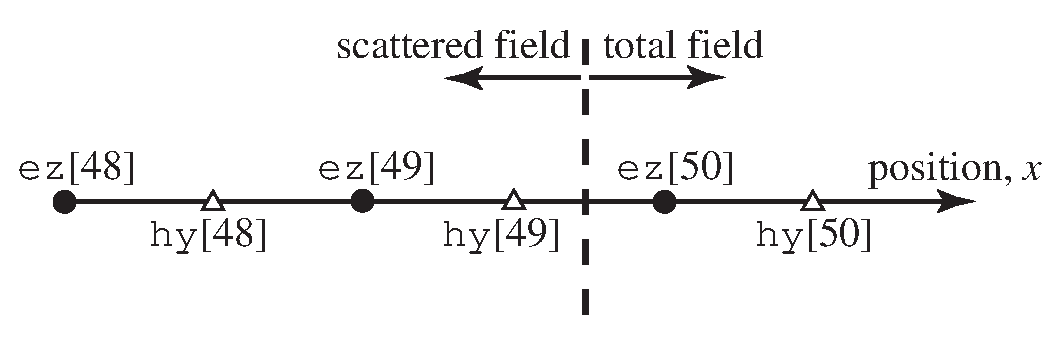
\epsfig{width=5.0in,file=Figures/Fdtd-intro/fdtd-1d-tfsf.eps}
  \end{center}
  \caption{Portion of the one-dimensional arrays in the vicinity of a
  total-field/scattered-field boundary.  Scattered field 
  exists to the left of the boundary and total field exists
  to the right.  Note that node {\tt hy[49]} has an index of $49$ in a
  computer program but corresponds logically to
  the location $(49+\half)\Delx$ or, equivalently, $(50-\half)\Delx$.
  \label{fig:tfsf} }
\end{figure}
Defining the scattered-field region to be to the left of the boundary
and the total-field region to be to the right, we see that {\tt
hy[49]} is the last node in the scattered-field region while {\tt
ez[50]} is the first node in the total-field region.

When updating the nodes adjacent to the boundary, there is a problem,
i.e., an inconsistency, in that a neighbor to one side is not the same
type of field as the field being updated.  This is to say that a
total-field node will depend on a scattered-field node and,
conversely, a scattered-field node will depend on a total-field node.
The solution to this problem actually provides the way in which fields
are introduced into the grid using the TFSF boundary.

Consider the usual update equation of the electric field at location
$m=50$ which was given in \refeq{eq:updateEz} and is repeated below
\begin{equation}
  \overbrace{\fdtd{E_z}{50}{q+1}}^{\mbox{\scriptsize tot}}
  =
  \overbrace{\fdtd{E_z}{50}{q}}^{\mbox{\scriptsize tot}} + 
  \frac{\Delt}{\epsilon\Delx}
   \left(
  \overbrace{\fdtdh{H_y}{50+\half}{q+\half}}^{\mbox{\scriptsize tot}} -
  \overbrace{\fdtdh{H_y}{50-\half}{q+\half}}^{\mbox{\scriptsize scat}}
  \right).
  \label{eq:updateEzTFSF}
\end{equation}
We have assumed the TFSF boundary is between $\fdtd{E_z}{50}{q+1}$
and $\fdtdh{H_y}{50-\half}{q+\half}$ and the labels above the individual
components indicate if the field is in the total-field region or the
scattered-field region.  We see that $\fdtd{E_z}{50}{q+1}$ and
$\fdtdh{H_y}{50+\half}{q+\half}$ are total-field nodes but
$\fdtdh{H_y}{50-\half}{q+\half}$ is a scattered-field node---it lacks
the incident field.  This can be fixed by adding the incident field to
$\fdtdh{H_y}{50-\half}{q+\half}$ in
\refeq{eq:updateEzTFSF}.  This added field must correspond to the
magnetic field which exists at location $50-1/2$ and time step
$q+1/2$.  Thus, a consistent update equation for $\fdtd{E_z}{50}{q+1}$
which only involves total fields is
\begin{eqnarray}
  \overbrace{\fdtd{E_z}{50}{q+1}}^{\mbox{\scriptsize tot}} &=&
  \overbrace{\fdtd{E_z}{50}{q}}^{\mbox{\scriptsize tot}} + {} \\
  &&\frac{\Delt}{\epsilon\Delx}
   \left(
   \overbrace{\fdtdh{H_y}{50+\half}{q+\half}}^{\mbox{\scriptsize tot}} -
   \overbrace{
   \left\{
   \overbrace{\fdtdh{H_y}{50-\half}{q+\half}}^{\mbox{\scriptsize scat}} +
   \overbrace{\left(
     -\frac{1}{\eta}\Einc\!\left[50-\half,q+\half\right]
   \right)}^{\mbox{\scriptsize inc}}
   \right\}}^{\mbox{\scriptsize tot}}\right).
   \nonumber
   \label{eq:updateEzTFSFI}
\end{eqnarray}
The sum of the terms in braces gives the total magnetic field for
$\fdtdh{H_y}{50-\half}{q+\half}$.  Note that here the incident field
is assumed to be given.  (It might be calculated analytically or, as
we will see in higher dimensions where the TFSF boundary involves
several points, it might be calculated with an auxilliary FDTD
simulation of its own.  But, either way, it is known.)

Instead of modifying the update equation, it is usually best to
preserve the standard update equation (so that it can be put in a loop
that pertains to all nodes), and then apply a correction in a separate
step.  In this way, $\fdtd{E_z}{50}{q+1}$ is updated in a two-step
process:
\begin{eqnarray}
  \fdtd{E_z}{50}{q+1} &=& \fdtd{E_z}{50}{q} + 
  \frac{\Delt}{\epsilon\Delx}
   \left(\fdtdh{H_y}{50+\half}{q+\half} -
         \fdtdh{H_y}{50-\half}{q+\half}\right), \\
  \fdtd{E_z}{50}{q+1} &=& \fdtd{E_z}{50}{q+1} + 
    \frac{\Delt}{\epsilon\Delx}
    \frac{1}{\eta}\Einc\!\left[50-\half,q+\half\right]. \label{eq:correction}
\end{eqnarray}
The characteristic impedance $\eta$ can be written as
$\sqrt{\mu_r\mu_0/\epsilon_r\epsilon_0}=
\eta_0\sqrt{\mu_r/\epsilon_r}$.  Recall from \refeq{eq:coefEz} that
the coefficient $\Delt/\epsilon\Delx$ can be expressed as $\eta_0
S_c/\epsilon_r$ where $S_c$ is the Courant number.  Combining these
terms, the correction equation \refeq{eq:correction} can be written
\begin{equation}
  \fdtd{E_z}{50}{q+1} = \fdtd{E_z}{50}{q+1} + 
    \frac{S_c}{\sqrt{\epsilon_r\mu_r}}\Einc\!\left[50-\half,q+\half\right].
  \label{eq:correctionI}
\end{equation}
With a Courant number of unity and free space (where
$\epsilon_r=\mu_r=1$), this reduces to
\begin{equation}
  \fdtd{E_z}{50}{q+1} = \fdtd{E_z}{50}{q+1} +
  \Einc\!\left[50-\half,q+\half\right]. \label{eq:correctionII} 
\end{equation}
This equation simply says that the incident field that existed
one-half a temporal step in the past and one-half a spatial step to
the left of $\fdtd{E_z}{50}{q+1}$ is added to this node.  This is
logical since a field traveling to the right requires one-half of a
temporal step to travel half a spatial step.

Now consider the update equation for $\fdtdh{H_y}{50-\half}{q+\half}$
which is given by \refeq{eq:updateHy} (with one subtracted from the
spatial offset):
\begin{equation}
  \overbrace{\fdtdh{H_y}{50-\half}{q+\half}}^{\mbox{\scriptsize scat}} = 
  \overbrace{\fdtdh{H_y}{50-\half}{q-\half}}^{\mbox{\scriptsize scat}} +
  \frac{\Delt}{\mu\Delx}
  \left(
  \overbrace{\fdtd{E_z}{50}{q}}^{\mbox{\scriptsize tot}} - 
  \overbrace{\fdtd{E_z}{49}{q}}^{\mbox{\scriptsize scat}}
  \right).
  \label{eq:updateHyTFSF}
\end{equation}
As was true for the update of the electric field adjacent to the TFSF
boundary, this is not a consistent equation since the terms are
scattered-field quantities except for $\fdtd{E_z}{50}{q}$ which is in
the total-field region.  To correct this, the incident field could be
subtracted from $\fdtd{E_z}{50}{q}$.  Rather than modifying
\refeq{eq:updateHyTFSF}, we choose to give the necessary correction as
a separate equation.  The correction would be
\begin{equation}
  \fdtdh{H_y}{50-\half}{q+\half} = \fdtdh{H_y}{50-\half}{q+\half} -
  \frac{\Delt}{\mu\Delx} \Einc[50,q].
  \label{eq:correctionHy}
\end{equation}
With a Courant number of unity and free space, this equation becomes
\begin{equation}
  \fdtdh{H_y}{50-\half}{q+\half} = \fdtdh{H_y}{50-\half}{q+\half} -
  \frac{1}{\eta_0} \Einc[50,q].
  \label{eq:correctionHyI}
\end{equation}

As mentioned previously, there is nothing that requires the origin to
be assigned to one particular node in the grid.  There is no reason
that one has to associate the location $x=0$ with the left end of the
grid.  In the TFSF formulation it is usually most convenient to fix
the origin relative to the TFSF boundary itself.  Let the origin $x=0$
correspond to the node $\fdtd{E_z}{50}{}$.  Such a shift requires that
$50$ be subtracted from the spatial indices given previously for the
incident field.  The correction equations thus become
\begin{eqnarray}
  \fdtdh{H_y}{50-\half}{q+\half} &=& \fdtdh{H_y}{50-\half}{q+\half} -
  \frac{1}{\eta_0} \Einc[0,q], 
  \label{eq:correctionHyFinal} 
  \\
  \fdtd{E_z}{50}{q+1} &=& \fdtd{E_z}{50}{q+1} +
  \Einc\!\left[-\half,q+\half\right]. 
  \label{eq:correctionEzFinal} 
\end{eqnarray}

To implement a TFSF boundary, one merely has to translate
\refeq{eq:correctionHyFinal} and \refeq{eq:correctionEzFinal} into the
necessary statements.  A program that implements a TFSF boundary
between {\tt hy[49]} and {\tt ez[50]} is shown in Program
\ref{pro:1Dtfsf}.
\begin{program}
{\tt 1Dtfsf.c}: \index{1Dtfsf.c@{\tt 1Dtfsf.c}}
One-dimensional simulation with a TFSF boundary between {\tt hy[49]}
and {\tt ez[50]}. \label{pro:1Dtfsf}
\codemiddle
\begin{lstlisting}
/* 1D FDTD simulation with a simple absorbing boundary condition
 * and a TFSF boundary between hy[49] and ez[50]. */

#include <stdio.h>
#include <math.h>

#define SIZE 200

int main()
{
  double ez[SIZE] = {0.}, hy[SIZE] = {0.}, imp0 = 377.0;
  int qTime, maxTime = 450, mm;

  char basename[80]="sim", filename[100];
  int frame = 0;
  FILE *snapshot;

  /* do time stepping */
  for (qTime = 0; qTime < maxTime; qTime++) {
/*b*/
    /* simple ABC for hy[size - 1] */
    hy[SIZE - 1] = hy[SIZE - 2];                   /*@ \label{1DtfsfC} @*/
/*n*/
    /* update magnetic field */
    for (mm = 0; mm < SIZE - 1; mm++)
      hy[mm] = hy[mm] + (ez[mm + 1] - ez[mm]) / imp0;
/*b*/
    /* correction for Hy adjacent to TFSF boundary */
    hy[49] -= exp(-(qTime - 30.) * (qTime - 30.) / 100.) / imp0; /*@ \label{1DtfsfA} @*/

    /* simple ABC for ez[0] */
    ez[0] = ez[1];                             /*@ \label{1DtfsfD} @*/
/*n*/
    /* update electric field */
    for (mm = 1; mm<SIZE; mm++)
      ez[mm] = ez[mm] + (hy[mm] - hy[mm - 1]) * imp0;
/*b*/
    /* correction for Ez adjacent to TFSF boundary */
    ez[50] += exp(-(qTime + 0.5 - (-0.5) - 30.) *    /*@ \label{1DtfsfB} @*/
                   (qTime + 0.5 - (-0.5) - 30.) / 100.);
/*n*/
    /* write snapshot if time a multiple of 10 */
    if (qTime % 10 == 0) {
      sprintf(filename, "%s.%d", basename, frame++);
      snapshot = fopen(filename, "w");
      for (mm = 0; mm < SIZE; mm++)
        fprintf(snapshot, "%g\n", ez[mm]);
      fclose(snapshot);
    }
  } /* end of time-stepping */

  return 0;
}
\end{lstlisting}
\end{program}
Note that this is similar to Program \ref{pro:1Dadditive}.  Other than
the incorporation of the ABC's in line \ref{1DtfsfC} and
\ref{1DtfsfD}, the only differences are the removal of the additive
source (line \ref{1DadditiveE} of Program \ref{pro:1Dadditive}) and
the addition of the two correction equations in lines \ref{1DtfsfA}
and \ref{1DtfsfB}.  The added code is shown in bold.  In line
\ref{1DtfsfB}, the half-step forward in time is obtained with {\tt
qTime+0.5}.  The half-step back in space is obtained with the {\tt
-0.5} which is enclosed in parentheses.

The waterfall plot of the fields generated by Program \ref{pro:1Dtfsf}
is shown in Fig.\ \ref{fig:waterfallTFSF}.  
\begin{figure}
  \begin{center}
  \epsfig{width=4.6in,file=Code/Fdtd-intro/waterfall-tfsf.eps}
  \end{center}
  \caption{Waterfall plot of the electric fields produced by
    Program \ref{pro:1Dtfsf} which has a TFSF boundary between nodes
    {\tt hy[49]} and {\tt ez[50]}.}
  \label{fig:waterfallTFSF}
\end{figure}
Note that the field appears at node 50 and travels exclusively to the
right---no field propagates to the left from the TFSF boundary.  Since
there is nothing to scatter the incident field in this simulation,
Fig.\ \ref{fig:waterfallTFSF} shows only the incident field.  The next
step is, thus, the inclusion of some inhomogeneity in the grid to
generate scattered fields.


\section{Inhomogeneities \label{sec:gridInhomogeneities}}

The FDTD update equations were obtained from approximations of
Faraday's and Ampere's laws which were themselves differential
equations.  Differential equations pertain at a point.  Thus, the
$\epsilon$ and $\mu$ which appear in these equations are the ones
which exist at the location of the corresponding node.  It is
certainly permissible that these values change from point to point.
In fact, it is required that they change when modeling inhomogeneous
material.

Recall, from \refeq{eq:coefEz}, that the electric-field update
equation had a coefficient of $\eta_0 S_c/\epsilon_r$.  Assuming that
the Courant number $S_c$ is still unity, but allowing the relative
permittivity to be a function of position, the update equation could
be implemented with a statement such as
\begin{verbatim}
  ez[m] = ez[m] + (hy[m] - hy[m-1])*imp0/epsR[m];
\end{verbatim}
where the array element {\tt epsR[m]} contains the relative
permittivity at the point $m\Delx$, i.e., at a point collocated with
the node {\tt ez[m]}.  The size of the {\tt epsR} array would be the
same size as the electric-field array and the elements have to be
initialized to appropriate values.

The same concept applies to the relative permeability in the updating
of the magnetic fields where the update coefficient is given by
$S_c/\mu_r\eta_0$ (ref.\ \refeq{eq:coefHy}).  The relative
permeability that exists at the point in space corresponding to the
location of a particular magnetic-field node is the one that should be
used in the update equation for that node.  Assuming an array {\tt
muR} has been created and initialized with the values of the relative
permeability, the magnetic-fields would be updated with an equation
such as
\begin{verbatim}
  hy[m] = hy[m] + (ez[m + 1] - ez[m]) / imp0 / muR[m];
\end{verbatim}

A program that models a region of space near the interface between
free space and a dielectric with a relative permittivity of nine is
shown in Program \ref{pro:1Ddielectric} (the permeability is that of
free space).  The incident field is still introduced via a TFSF
boundary, which is in the free-space side of the computational domain,
and the ABC on the left hand side is the same as before.  However,
there are some other minor changes between this program and the
program in Program \ref{pro:1Dtfsf}.  The electric and magnetic fields
are no longer initialized when they are declared.  Instead, two loops
are used to set the initial fields to zero.  The magnetic field is now
declared to have one fewer node than the electric field.  This was
done so that the computational domain begins and ends on an
electric-field node.  (There are no truly compelling reasons to have
the computational domain begin and end with the same field type, but
such symmetry can simplify coding and some aspects of certain
problems.)  Because the grid now terminates on an electric field, the
ABC at the right end of the grid must be applied to this terminal
electric-field node.  This is accomplished with the statement in line
\ref{1DdielectricB}.

\begin{program}
{\tt 1Ddielectric.c}: \index{1Ddielectric.c@{\tt 1Ddielectric.c}}
One-dimensional FDTD program to model an interface between free-space
and a dielectric that has a relative permittivity $\epsilon_r$ of
$9$. \label{pro:1Ddielectric}
\codemiddle
\begin{lstlisting}
/* 1D FDTD simulation with a simple absorbing boundary
 * condition, a TFSF boundary between hy[49] and ez[50], and
 * a dielectric material starting at ez[100] */

#include <stdio.h>
#include <math.h>

#define SIZE 200

int main()
{
  double ez[SIZE], hy[SIZE - 1], epsR[SIZE], imp0 = 377.0;
  int qTime, maxTime = 450, mm;
  char basename[80] = "sim", filename[100];
  int frame = 0;
  FILE *snapshot;
/*b*/
  /* initialize electric field */
  for (mm = 0; mm < SIZE; mm++)
    ez[mm] = 0.0;

  /* initialize magnetic field */
  for (mm = 0; mm < SIZE - 1; mm++)
    hy[mm] = 0.0;

  /* set relative permittivity */
  for (mm = 0; mm < SIZE; mm++) /*@ \label{1DdielectricA} @*/
    if (mm < 100)
      epsR[mm] = 1.0;
    else
      epsR[mm] = 9.0;
/*n*/
  /* do time stepping */
  for (qTime = 0; qTime < maxTime; qTime++) {

    /* update magnetic field */
    for (mm = 0; mm<SIZE - 1; mm++)
      hy[mm] = hy[mm] + (ez[mm + 1] - ez[mm]) / imp0;

    /* correction for Hy adjacent to TFSF boundary */
    hy[49] -= exp(-(qTime - 30.) * (qTime - 30.) / 100.) / imp0;

    /* simple ABC for ez[0] and ez[SIZE - 1] */
    ez[0] = ez[1];
/*b*/    ez[SIZE-1] = ez[SIZE-2]; /*@ \label{1DdielectricB} @*/
/*n*/
    /* update electric field */
    for (mm = 1; mm < SIZE - 1; mm++)
/*b*/      ez[mm] = ez[mm] + (hy[mm] - hy[mm - 1]) * imp0 / epsR[mm];
/*n*/
    /* correction for Ez adjacent to TFSF boundary */
    ez[50] += exp(-(qTime + 0.5 - (-0.5) - 30.)*
                   (qTime + 0.5 - (-0.5) - 30.) / 100.);

    /* write snapshot if time a multiple of 10 */
    if (qTime % 10 == 0) {
      sprintf(filename, "%s.%d", basename, frame++);
      snapshot = fopen(filename, "w");
      for (mm = 0; mm < SIZE; mm++)
        fprintf(snapshot, "%g\n", ez[mm]);
      fclose(snapshot);
    }
  } /* end of time-stepping */

  return 0;
}
\end{lstlisting}
\end{program}

The relative-permittivity array {\tt epsR} is initialize in the loop
starting at line \ref{1DdielectricA}.  If the spatial index {\tt mm} is
less than $100$, the relative permittivity is set to unity (i.e., free
space), otherwise it is set to $9$.  The characteristic impedance of
free space is $\eta_0$ while the impedance for the dielectric is
$\eta_0/3$.  Note that the update equations do not directly
incorporate the dielectric impedance.  Rather, the coefficient that
appears in the equation uses the impedance of free space and the
relative permittivity that pertains at that point.

When a wave is normally incident from a medium with a characteristic
impedance $\eta_1$ to a medium with a characteristic impedance
$\eta_2$, the reflection coefficient $\Gamma$ and the transmission
coefficient $T$ are given by
\begin{eqnarray}
 \Gamma &=& \frac{\eta_2 - \eta_1}{\eta_2 + \eta_1}, \label{eq:gamma}\\
      T &=& \frac{2 \eta_2}{\eta_2 + \eta_1}.
\end{eqnarray}
Therefore the reflection and transmission coefficients
that pertain to this example are
\begin{eqnarray}
  \Gamma &=& \frac{\eta_0/3 - \eta_0}{\eta_0/3 + \eta_0} =
            -\frac{1}{2}, \\
  T &=& \frac{2 \eta_0/3}{\eta_0/3 + \eta_0} = \frac{1}{2}.
\end{eqnarray}

The waterfall plot of the data produced by Program
\ref{pro:1Ddielectric} is shown in Fig.\ \ref{fig:waterfallDielec}.
\begin{figure}
  \begin{center}
  \epsfig{width=4.6in,file=Code/Fdtd-intro/waterfall-dielec.eps}
  \end{center}
  \caption{Waterfall plot of the electric fields produced by Program
  \ref{pro:1Ddielectric} which has a dielectric with a relative
  permittivity of $9$ starting at node $100$.  Free space is to the
  left of that.}  \label{fig:waterfallDielec}
\end{figure}
Once the field encounters the interface at node $100$, a reflected
field (i.e., a scattered field) is created.  Although one cannot
easily judge scales from the waterfall plot, it can be seen that the
reflected field is negative and appears to have about half the
magnitude of the incident pulse (the peak of the incident field spans
a vertical space corresponding to nearly two frames while the peak of
the reflected field spans about one frame).  Similarly, the
transmitted pulse is positive and appears to have half the magnitude
of the incident field.  One can see this more clearly in Fig.\
\ref{fig:1DdiectricSnaps} which shows the field at time-steps $100$
and $140$.  The incident pulse had unit amplitude.  At the time-steps
shown here, the field has split into the transmitted and reflected
pulses, each of which has an magnitude of one-half.
\begin{figure}
  \begin{center}
  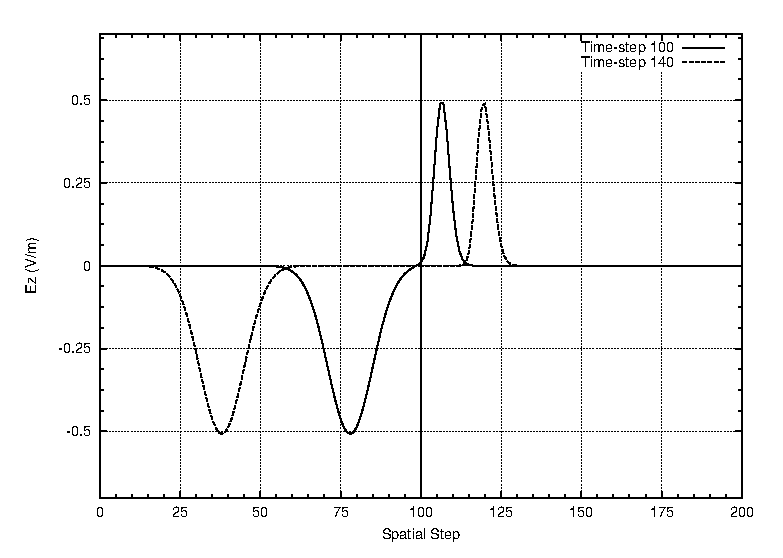
\epsfig{width=4.6in,file=Code/Fdtd-intro/dielectric.eps}
  \end{center}
  \caption{Two of the snapshots produced by Program
  \ref{pro:1Ddielectric}.  The vertical line at node $100$ corresponds
  to the interface between free space and the dielectric.  The
  incident pulse had unit amplitude.  Shown in this figure are the
  transmitted field (to the right of the interface) and the reflected
  field (to the left).}  \label{fig:1DdiectricSnaps}
\end{figure}

Returning to the waterfall plot of Fig.\ \ref{fig:waterfallDielec},
one can also see that the pulse in the dielectric travels more slowly
than the pulse in free space.  With a relative permittivity of $9$,
the speed of light should be one-third of that in free space.  Thus,
from frame to frame the peak in the dielectric has moved one-third of
the distance that the peak moves in free space.

There are two numerical artifacts present in Fig.\
\ref{fig:waterfallDielec}, one which we need to fix and the other we
need to understand.  Note that when the reflected field encounters the
left boundary it disappears.  The ABC does its job and the field is
absorbed.  On the other hand, when the transmitted wave encounters the
right boundary, at approximately frame $37$, it is not completely
absorbed.  A reflected wave is produced which is visible in the upper
right-hand corner of Fig.\ \ref{fig:waterfallDielec}.  Why is the ABC
no longer working?  The problem is that the simple ABC used so far is
based on the assumption that the wave travels one spatial step for
every time step.  In this dielectric, with a relative permittivity of
$9$, the speed of light is one-third that of free space and hence the
wave does not travel one spatial step per time step---it travels a
third of a spatial step.  A possible fix might be to update the
electric field on the boundary with the value of the neighboring
electric-field node from three time steps in the past.  However, what
if the relative permittivity of the dielectric were $2$?  In that case
the speed of light would be $1/\sqrt{2}$ times that of free space.
There would be no past value of an interior node that could be used
directly to update the boundary node.  So, it is necessary to rethink
the implementation of the ABC so that it can handle these sorts of
situations.  This will be addressed in another chapter.

The other artifact present in Fig.\ \ref{fig:waterfallDielec} is
slightly less obvious.  If you look at the trailing edge of the
transmitted pulse around frame $33$, or so, you will see a slight
wiggle.  The incident field is a Gaussian pulse which asymptotically
goes to zero to either side of the peak value.  However, the
transmitted pulse does not behave this way---at least not after
propagating in the dielectric for a while (initially there are no
wiggles visible at the trailing edge of the transmitted pulse).  These
wiggles are caused by {\em dispersion}
\index{dispersion}
in the FDTD grid.  When the Courant number is anything other than
unity, the FDTD grid is dispersive, meaning that different frequencies
propagate at different speeds.  Note that we have defined the Courant
number as the $c\Delt/\Delx$ where $c$ is the speed of light in free
space.  We will generally maintain the convention that $c$ represents
the speed of light in free space.  However, one can think of the
Courant number as a local quantity that equals the local speed of
light multiplied by the ratio $\Delt/\Delx$.
\index{Courant number!local variation}
Because the speed of light is one-third of that of free space, the
local Courant number in the dielectric is not unity.  Since the
Gaussian pulse consists of a range of frequencies, and these
frequencies are propagating at different speeds, the pulse ``breaks
apart'' as it propagates.  In practice, one tries to ensure that the
amount of dispersion is small, but it is unavoidable in
multi-dimensional FDTD analysis.  Dispersion will be considered
further later.

Because of the discretized nature of the FDTD grid, the location of a
material boundary can be somewhat ambiguous.  The relatively
permittivity that pertains to a particular electric-field node can be
assumed to exist over the space that extends from one of its
neighboring magnetic-field nodes to the other neighboring
magnetic-field node.  This idea is illustrated in Fig.\
\ref{fig:abrupt} which shows a portion of the FDTD grid together with
the permittivity associated with each node.  The permittivities are
indicated with the bar along the bottom of the figure.  

If there is only a change in permittivity, the location of the
interface between the different media seems rather clear.  It
coincides with the magnetic-field node that has $\epsilon_1$ to one
side and $\epsilon_2$ to the other.  However, what if there is a
change in permeability too?  The permeabilities are indicated with a
bar along the top of the figure.  It is seen that the interface
associated with the change in permeabilities is not aligned with the
interface associated with the change in permittivities.  One way to
address this problem is to assume the true interface is aligned with
an electric-field node.  This node would then use the average of the
permittivities of the media to either side.  This scenario is depicted
in Fig.\ \ref{fig:average}.  Alternatively, if one wants to have the
boundary aligned with a magnetic-field node, then the node located on
the boundary would use the average of the permeabilities to either
side while the electric-field nodes would use the permittivity of the
first medium if they were to the left of the boundary and use the
permittivity of the second medium if they were to the right.

\begin{figure}
  \begin{center}
  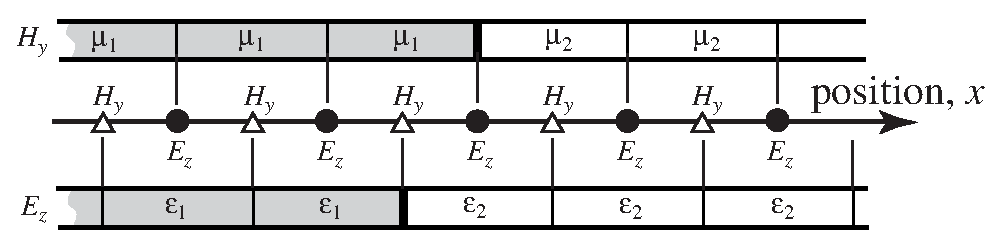
\epsfig{width=5.in,file=Figures/Fdtd-intro/abrupt-boundaries.eps}
  \end{center}
  \caption{One-dimensional grid depicting an abrupt change in both the
  permittivity and permeability.  The actual location of the interface
  between the two media is ambiguous.}
  \label{fig:abrupt}
\end{figure}

\begin{figure}
  \begin{center}
  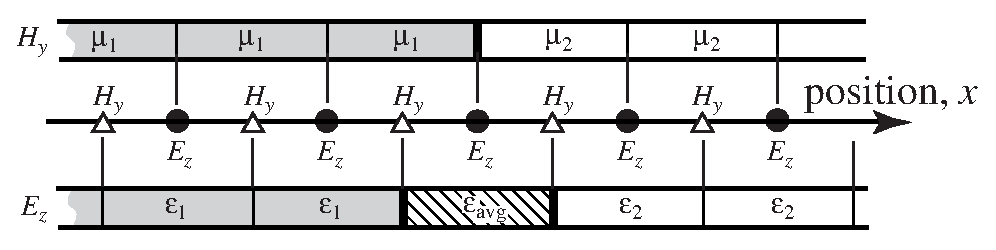
\epsfig{width=5.in,file=Figures/Fdtd-intro/avg-boundaries.eps}
  \end{center}
  \caption{One-dimensional grid depicting a change from one medium to
  another.  An electric-field node is assumed to be collocated with
  the interface, hence the permittivity used there is the average of
  the permittivities to either side.}
  \label{fig:average}
\end{figure}


\section{Lossy Material \label{sec:loss}}

When a material has a finite conductivity $\sigma$, a
conduction-current term is added to Ampere's law (which is distinct
from the source-current term mentioned in Sec.\ \ref{sec:additive}).
Thus,
\begin{equation}
  \sigma\Evec + \epsilon \frac{\partial \Evec}{\partial t} =
  \nabla \times \Hvec.
\end{equation}
The discretized form of Ampere's law provided the update equation for
the electric field.  As before, assuming only a $z$ component of the
field and variation only in the $x$ direction, this equation reduces to
\begin{equation}
  \sigma E_z + \epsilon \frac{\partial E_z}{\partial t} =
    \frac{\partial H_y}{\partial x}.
  \label{eq:ampereLoss}
\end{equation}
As discussed in Sec.\ \ref{sec:update} and detailed in Fig.\
\ref{fig:spaceTimeUpdate}, this equation was expanded about the point
$(m\Delx,(q+1/2)\Delt)$ to obtain the electric-field update equation.
However, when loss is present, the undifferentiated electric field
appears on the left side of the equation.  With the assumed
arrangement of the nodes shown in Fig.\ \ref{fig:spaceTimeUpdate},
there is no electric field at the space-time point
$(m\Delx,(q+1/2)\Delt)$.  This problem can be circumvented by using
the averaging (in time) of the electric field to either side of the
desired point, i.e.,
\begin{equation}
  \fdtd{E_z}{m}{q+\half} \approx 
  \frac{\fdtd{E_z}{m}{q+1}+\fdtd{E_z}{m}{q}}{2}.
\end{equation}
Thus a suitable discretization of Ampere's law when loss is present is
\begin{equation}
  \sigma \frac{\fdtd{E_z}{m}{q+1}+\fdtd{E_z}{m}{q}}{2} +
  \epsilon\frac{\fdtd{E_z}{m}{q+1} - \fdtd{E_z}{m}{q}}{\Delt} = 
  \frac{\fdtdh{H_y}{m+\half}{q+\half} - \fdtdh{H_y}{m-\half}{q+\half}}{\Delx}.
\end{equation}
As before, this can be solved for $\fdtd{E_z}{m}{q+1}$, which is the
``future'' field, in terms of purely past fields.  The result is
\begin{equation}
  \fdtd{E_z}{m}{q+1}=
  \frac{1-\frac{\sigma\Delt}{2\epsilon}}{1+\frac{\sigma\Delt}{2\epsilon}}
  \fdtd{E_z}{m}{q} +
  \frac{\frac{\Delt}{\epsilon\Delx}}{1+\frac{\sigma\Delt}{2\epsilon}}
  \left(\fdtdh{H_y}{m+\half}{q+\half} - \fdtdh{H_y}{m-\half}{q+\half}\right).
  \label{eq:updateEzLoss}
\end{equation}
When $\sigma$ is zero this reduces to the previous update equation
\refeq{eq:updateEz}.

In previous update equations it was possible to express the
coefficients in terms of the Courant number, i.e., the ratio of the
temporal step to the spatial step.  In \refeq{eq:updateEzLoss} it
appears the term $\sigma\Delt/2\epsilon$ requires that the temporal
step be specified (together with the conductivity and permittivity).
However, there is a way to express this such that the temporal step
does not need to be stated explicitly.  This will be considered in
detail in Sec.\ \ref{sec:conductivity}.

As we will see, it is occasionally helpful to incorporate a magnetic
conduction current in Faraday's law.  Similar to the electric
conduction current, the magnetic conduction current is assumed to be
the product of the magnetic conductivity $\sigma_m$ and the magnetic
field.  Faraday's law becomes
\begin{equation}
  -\sigma_m\Hvec - \mu \frac{\partial \Hvec}{\partial t} =
  \nabla \times \Evec.
\end{equation}
We again restrict consideration to an $H_y$ component which varies
only in the $x$ direction.  This reduces to
\begin{equation}
  \sigma_m H_y + \mu \frac{\partial H_y}{\partial t} =
    \frac{\partial E_z}{\partial x}.
  \label{eq:faradayLoss}
\end{equation}
As before, this is expanded/discretized at the space-time point
$((m+1/2)\Delx,q\Delt)$.  Since there is no magnetic field available
at integer time steps, the magnetic field is averaged in time to
get an approximation of the field at time $q\Delt$.  This yields
\begin{eqnarray}
  \sigma_m\frac{\fdtdh{H_y}{m+\half}{q+\half}+\fdtdh{H_y}{m+\half}{q-\half}}{2} +
  \mu\frac{\fdtdh{H_y}{m+\half}{q+\half} - \fdtdh{H_y}{m+\half}{q-\half}}{\Delt}
  &=& \nonumber\\
  \frac{\fdtd{E_z}{m+1}{q} - \fdtd{E_z}{m}{q}}{\Delx}. &&
\end{eqnarray}
Solving for $\fdtdh{H_y}{m+\half}{q+\half}$ yields the update equation
\begin{equation}
  \fdtdh{H_y}{m+\half}{q+\half}=
  \frac{1-\frac{\sigma_m\Delt}{2\mu}}{1+\frac{\sigma_m\Delt}{2\mu}}
  \fdtdh{H_y}{m+\half}{q-\half} +
  \frac{\frac{\Delt}{\mu\Delx}}{1+\frac{\sigma_m\Delt}{2\mu}}
  \left(\fdtd{E_z}{m+1}{q} - \fdtd{E_z}{m}{q}\right).
  \label{eq:updateHyLoss}
\end{equation}
When $\sigma_m$ is zero this reduces to \refeq{eq:updateHy}.

Program \ref{pro:1Dlossy} models a lossy dielectric half-space that
starts at node $100$.  As before, the relative permittivity is $9$.
However there is also an electric loss present such that
$\sigma\Delt/2\epsilon$ is $0.01$.  The program uses two coefficient
arrays, {\tt ceze} and {\tt cezh}.  The terms in the {\tt ceze} array
multiply the previous (or ``self'') term while the {\tt cezh} array
contains the terms that multiply the spatial difference of the
magnetic fields.  Think of these arrays as consisting of coefficients
(or constants), hence the ``{\tt c}'' at the start of their name, that
appear in the $E_z$ update equation, hence the {\tt ez} part of the
name, and multiplying either the electric field ({\tt ceze}) or the
magnetic field ({\tt cezh}).  The values of these arrays are set in
the loop that starts at line \ref{1DlossyA}.  Since the simple ABC
previously employed at the right edge of the grid does not work, it
has been removed but the left side of the grid is terminated as
before.  The magnetic field update is unchanged from before.  A
waterfall plot of the data produced by Program
\ref{pro:1Dlossy} is shown in Fig.\ \ref{fig:waterfallLoss}.  The pulse
decays as it propagates in the lossy region and eventually decays to a
rather negligible value.  Thus the lack of an ABC at the right side of
the grid is not really a concern in this particular instance.
\begin{program}
{\tt 1Dlossy.c}: \index{1Dlossy.c@{\tt 1Dlossy.c}}
One-dimensional simulation with a lossy dielectric
region. \label{pro:1Dlossy}
\codemiddle
\begin{lstlisting}
/* 1D FDTD simulation of a lossy dielectric region. */

#include <stdio.h>
#include <math.h>

#define SIZE 200
#define LOSS 0.01

int main()
{
  double ez[SIZE], hy[SIZE - 1], ceze[SIZE], cezh[SIZE],
    imp0 = 377.0;
  int qTime, maxTime = 450, mm;
  char basename[80] = "sim", filename[100];
  int frame = 0;
  FILE *snapshot;

  /* initialize electric field */
  for (mm = 0; mm < SIZE; mm++)
    ez[mm] = 0.0;

  /* initialize magnetic field */
  for (mm = 0; mm < SIZE - 1; mm++)
    hy[mm] = 0.0;

  /* set electric-field update coefficients */
  for (mm = 0; mm < SIZE; mm++)      /*@ \label{1DlossyA} @*/
    if (mm < 100) { /* free space */
      ceze[mm] = 1.0;
      cezh[mm] = imp0;
    } else {     /* lossy dielectric */
      ceze[mm] = (1.0 - LOSS) / (1.0 + LOSS);
      cezh[mm] = imp0 / 9.0 / (1.0 + LOSS);
    }

  /* do time stepping */
  for (qTime = 0; qTime < maxTime; qTime++) {

    /* update magnetic field */
    for (mm = 0; mm < SIZE - 1; mm++)
      hy[mm] = hy[mm] + (ez[mm + 1] - ez[mm]) / imp0;

    /* correction for Hy adjacent to TFSF boundary */
    hy[49] -= exp(-(qTime - 30.) * (qTime - 30.) / 100.) / imp0;

    /* simple ABC for ez[0] */
    ez[0] = ez[1];

    /* update electric field */
    for (mm = 1; mm < SIZE - 1; mm++)
      ez[mm] = ceze[mm] * ez[mm] + cezh[mm] * (hy[mm] - hy[mm - 1]);

    /* correction for Ez adjacent to TFSF boundary */
    ez[50] += exp(-(qTime + 0.5 - (-0.5) - 30.) *
                   (qTime + 0.5 - (-0.5) - 30.) / 100.);

    /* write snapshot if time a multiple of 10 */
    if (qTime % 10 == 0) {
      sprintf(filename, "%s.%d", basename, frame++);
      snapshot=fopen(filename, "w");
      for (mm = 0; mm < SIZE; mm++)
        fprintf(snapshot, "%g\n", ez[mm]);
      fclose(snapshot);
    }
  } /* end of time-stepping */

  return 0;
}
\end{lstlisting}
\end{program}

\begin{figure}
  \begin{center}
  \epsfig{width=4.6in,file=Code/Fdtd-intro/waterfall-loss.eps}
  \end{center}
  \caption{Waterfall plot of the electric fields produced by Program
  \ref{pro:1Dlossy} which has a lossy dielectric region with a relative
  permittivity of $9$ starting at node $100$.}
  \label{fig:waterfallLoss}
\end{figure}

When loss is present the characteristic impedance of the medium
becomes
\begin{equation}
\eta = \sqrt{
       \frac{\mu\left(1-j\frac{\sigma_m}{\omega\mu}\right)}
            {\epsilon\left(1-j\frac{\sigma}{\omega\epsilon}\right)}}
     =  \eta_0\sqrt{
       \frac{\mu_r\left(1-j\frac{\sigma_m}{\omega\mu}\right)}
            {\epsilon_r\left(1-j\frac{\sigma}{\omega\epsilon}\right)}}
\end{equation}
When $\sigma_m/\mu = \sigma/\epsilon$ the terms in
parentheses are equal and hence cancel.  With those terms canceled,
the characteristic impedance is indistinguishable from the lossless
case.  Therefore
\begin{equation}
  \left.\eta\right|_{\frac{\sigma_m}{\mu} = \frac{\sigma}{\epsilon}}
  = \left.\eta\right|_{\sigma_m = \sigma = 0}
  = \eta_0 \sqrt{\frac{\mu_r}{\epsilon_r}}.
\end{equation}

As shown in \refeq{eq:gamma}, the reflection coefficient for a wave
normally incident on a planar boundary is proportional to the
difference of the impedances to either side of the interface.  If the
material on one side is lossless while the material on the other side
is lossy with $\sigma_m/\mu = \sigma/\epsilon$, then the impedances
are matched provided the ratios of $\epsilon_r$ and $\mu_r$ are also
matched across the boundary.  With the impedances matched, there will
be no reflection from the interface.  Therefore a lossy layer could be
used to terminate the grid.  The fields will dissipate in this lossy
region and, if the region is large enough, may be small by the time
they encounter the end of the grid.  Upon reflection from the end of
the grid, the fields would have to propagate back through the lossy
layer where they would decay even further.  With proper design the
reflected fields can be made inconsequentially small when they
eventually get back to the lossless portion of the grid.

A lossy layer with the impedance matched to the previous region can be
implemented easily in one dimension.  Program \ref{pro:1Dmatched} shows
a program where a lossless dielectric layer with $\epsilon_r=9$ starts
at node $100$.  The lossless region extends to node $180$.  At node
$180$, and beyond, the material has both a nonzero electric and a
magnetic conductivity.  The conductivities are matched in the sense
that $\sigma_m/\mu = \sigma/\epsilon$.  Thus the terms
$\sigma_m\Delt/2\mu$ and $\sigma\Delt/2\epsilon$ in the
update-equations are also matched.  In this program these terms are
set to $0.02$.  The coefficients used in the magnetic-field update
equations are stored in the arrays {\tt chyh} and {\tt chye}.


The waterfall plot of the data generated by Program
\ref{pro:1Dmatched} is shown in Fig.\ \ref{fig:waterfallMatched}.  The
fields that enter the lossless region propagate to the right and
eventually encounter the lossy region.  Because the impedances of the
lossless and lossy media are matched, the fields enter the lossy
region without reflection (actually, that is true in the continuous
world, but only approximately true in the discretized FDTD
world---there is some small reflection present).  As the fields
propagate in the lossy region they dissipate to the point where they
are almost negligible when they reenter the lossless region.  There is
no reflected field evident in the upper right corner of the plot.

\begin{program}
{\tt 1Dmatched.c}: \index{1Dmatched.c@{\tt 1Dmatched.c}}
Program with a lossless dielectric region followed by a lossy layer
that has its impedance matched to the lossless
dielectric. \label{pro:1Dmatched}
\codemiddle
\begin{lstlisting}
/* 1D FDTD simulation of a lossless dielectric region
 * followed by a lossy layer which matches the impedance
 * of the dielectric.  */

#include <stdio.h>
#include <math.h>

#define SIZE 200
#define LOSS 0.02
#define LOSS_LAYER 180

int main()
{
  double ez[SIZE], hy[SIZE - 1], ceze[SIZE], cezh[SIZE],
    chyh[SIZE - 1], chye[SIZE - 1], imp0 = 377.0;
  int qTime, maxTime = 450, mm;
  char basename[80] = "sim", filename[100];
  int frame = 0;
  FILE *snapshot;

  /* initialize electric field */
  for (mm = 0; mm < SIZE; mm++)
    ez[mm] = 0.0;

  /* initialize magnetic field */
  for (mm = 0; mm < SIZE - 1; mm++)
    hy[mm] = 0.0;

  /* set electric-field update coefficients */
  for (mm = 0; mm < SIZE; mm++)
    if (mm < 100) {
      ceze[mm] = 1.0;
      cezh[mm] = imp0;
    } else if (mm < LOSS_LAYER) {
      ceze[mm] = 1.0;
      cezh[mm] = imp0 / 9.0;
    } else {
      ceze[mm] = (1.0 - LOSS) / (1.0 + LOSS);
      cezh[mm] = imp0 / 9.0 / (1.0 + LOSS);
    }

  /* set magnetic-field update coefficients */
  for (mm = 0; mm < SIZE - 1; mm++)
    if (mm < LOSS_LAYER) {
      chyh[mm] = 1.0;
      chye[mm] = 1.0 / imp0;
    } else {
      chyh[mm] = (1.0 - LOSS) / (1.0 + LOSS);
      chye[mm] = 1.0 / imp0 / (1.0 + LOSS);
    }

  /* do time stepping */
  for (qTime = 0; qTime < maxTime; qTime++) {

    /* update magnetic field */
    for (mm = 0; mm < SIZE - 1; mm++)
      hy[mm] = chyh[mm] * hy[mm] + 
                  chye[mm] * (ez[mm + 1] - ez[mm]);

    /* correction for Hy adjacent to TFSF boundary */
    hy[49] -= exp(-(qTime - 30.) * (qTime - 30.) / 100.) / imp0;

    /* simple ABC for ez[0] */
    ez[0] = ez[1];

    /* update electric field */
    for (mm = 1; mm < SIZE - 1; mm++)
      ez[mm] = ceze[mm] * ez[mm] +
                  cezh[mm] * (hy[mm] - hy[mm - 1]);

    /* correction for Ez adjacent to TFSF boundary */
    ez[50] += exp(-(qTime + 0.5 - (-0.5) - 30.)*
                   (qTime + 0.5 - (-0.5) - 30.) / 100.);

    /* write snapshot if time a multiple of 10 */
    if (qTime % 10 == 0) {
      sprintf(filename, "%s.%d", basename, frame++);
      snapshot=fopen(filename, "w");
      for (mm = 0; mm < SIZE; mm++)
        fprintf(snapshot, "%g\n", ez[mm]);
      fclose(snapshot);
    }
  } /* end of time-stepping */

  return 0;
}
\end{lstlisting}
\end{program}

\begin{figure}
  \begin{center}
  \epsfig{width=4.6in,file=Code/Fdtd-intro/waterfall-matched-loss.eps}
  \end{center} \caption{Waterfall plot of the electric fields produced
  by Program \ref{pro:1Dmatched} which has a dielectric region
  starting at node $100$ with a relative permittivity of $9$.  This
  lossless region is followed by a lossy layer with matched impedance.
  The lossy region starts at node $180$.}
  \label{fig:waterfallMatched}
\end{figure}

\chapter{Improving the FDTD Code \label{chap:fdtdImproved}} 

%\setcounter{page}{1}

\renewcommand{\thefootnote}{\fnsymbol{footnote}}
\footnotetext{Lecture notes by John Schneider.  {\tt
fdtd-improved-code.tex}}

\section{Introduction}

The C code presented in the previous chapter adequately served its
purpose---it implemented the desired FDTD functionality in a
relatively straightforward way.  However, as the algorithms get more
involved, for instance, when implementing simulations of two- or
three-dimensional problems, the readability, portability, and
maintainability will be improved if our implementation is slightly
more sophisticated.  In this chapter we will implement the algorithms
of the previous chapter in a way which may seem, at first, to be
overly complicated.  However, as the complexity of the algorithms
increases in coming chapters, we will see that the effort required to
understand this more sophisticated approach will have been worth it.

%%%%%%%%%%%%%%%%%%%%%%%%%%%%%%%%%%%%%%%%%%%%%%%%%%%%%%%%%%%%%%%%%%%%%%%%%%%
\section{Arrays and Dynamic Memory
  Allocation \label{sec:memAllocation}} 

\index{memory allocation|(}
In C an array is stored in a block of contiguous memory.  Memory
itself is fundamentally a one-dimensional quantity since memory is
ultimately accessed with a single memory address.  Let us consider a
one-dimensional array of doubles {\tt ez} where the size is specified
at run-time rather than at compile-time.  The compiler needs to know
about the existence of this array, but at compile-time it does not
need to know the amount or the location of memory where the array will
be stored.  We can specify the size of the array when the program is
run and we can allow the computer to decide the location of the
necessary amount of memory.  The compiler is told about the potential
existence of the array with a pointer\index{pointers}.  Once the
pointer is associated with the appropriate block of memory, it is
virtually indistinguishable from a one-dimensional array.

The code shown in Fragment \ref{frag:oneDDynamic} demonstrates how the
array {\tt ez} can be created at run-time.  In line \ref{callocA} {\tt
ez} is declared as a pointer---it can store an address but when the
program initially starts it does not point to anything meaningful.
Line \ref{callocB} declares two integer variables: {\tt num\_elements}
which will contain the number of elements in the array, and {\tt mm}
which will be used as a loop counter.  Lines \ref{callocC} and
\ref{callocD} determine the number of elements the user desires.

\begin{fragment}
Fragment of code demonstrating how the size of the array {\tt ez} can
be set at run-time.  The header file {\tt stdlib.h} would typically
have to be included to provide the prototype for the {\tt calloc()}
function. \label{frag:oneDDynamic}
\codemiddle
\begin{lstlisting}
  double *ez;                /*@ \label{callocA} @*/
  int num_elements, mm;      /*@ \label{callocB} @*/

  printf("Enter the size of the array: ");  /*@ \label{callocC} @*/
  scanf("%d", &num_elements);               /*@ \label{callocD} @*/

  ez = calloc(num_elements, sizeof(double)); /*@ \label{callocE} @*/

  for (mm=0; mm < num_elements; mm++) /*@ \label{callocF} @*/
    ez[mm] = 3.0 * mm;                /*@ \label{callocG} @*/
\end{lstlisting}
\end{fragment}

Line \ref{callocE} is the key to getting {\tt ez} to behave as an
array.  In this line the pointer {\tt ez} is set equal to the memory
address that is returned by the function {\tt calloc()}.\footnote{{\tt
calloc()} is closely related to the function {\tt malloc()} which also
allocates a block of memory and returns the address of the start of
that block.  However {\tt calloc()} returns memory which has been
cleared, i.e., set to zero, while {\tt malloc()} returns memory which
may contain anything.  Since we want the field arrays initially to be
zero, it is better to use {\tt calloc()} than {\tt malloc()}.}
\index{calloc@{\tt calloc()}} {\tt calloc()} takes two arguments.  The
first specifies the number of elements in the array while the
second specifies the amount of memory needed for a single
element.  Here the {\tt sizeof()} operator is used to obtain the size
of a double variable.  (Although not shown in this fragment, when
using the {\tt calloc()} function one typically has to include the
header file {\tt stdlib.h} to provide the function prototype.)  If
{\tt calloc()} is unable to provide the requested memory it will
return {\tt NULL}.
\footnote{Robust code would check the return value and take appropriate
measures if {\tt NULL} were returned.  For now we will assume that
{\tt calloc()} succeeded.}

After the call of {\tt calloc()} in line \ref{callocE}, {\tt ez}
points to the start of a contiguous block of memory where the array
elements can be stored.  To demonstrate this, lines \ref{callocF} and
\ref{callocG} write the value of three times the array index to each
element of the array (so that {\tt ez[0]} would be $0.0$, {\tt ez[1]}
would be $3.0$, {\tt ez[2]} would be $6.0$, and so on).
\index{memory allocation|)}

Some compilers will actually complain about the code as it is written
in Fragment \ref{frag:oneDDynamic}.  The ``problem'' is that
technically {\tt calloc()} returns a void pointer---it is simply the
address of the start of a block of memory, but we have not said what is
stored at that memory.  We want a pointer to doubles since we will be
storing double precision variables in this memory.  The compiler
really already knows this since we are storing the address in {\tt ez}
which is a pointer to doubles.  Nevertheless, some compilers will give
a warning because of line \ref{callocE}.  Therefore, to ensure that
compilers do not complain, it would be best to replace line
\ref{callocE} with
\begin{code}
  ez = (double *)calloc(num_elements, sizeof(double));
\end{code}
In this way the void pointer returned by {\tt calloc()} is converted
(or cast) to a pointer to doubles.

\section{Macros \label{sec:macros}}

\index{macros|(}
C provides a preprocessor which ``processes'' your code prior to the
compiler itself.  Preprocessor directives start with the pound sign
({\tt \#}) and instruct the preprocessor to do things such as
include a header file (with an {\tt \#include} statement) or
substitute one string for another.  Program \ref{pro:1DbareBones}
had three preprocessor directives.  Two were used to include the files
{\tt stdio.h} and {\tt math.h} and one used a {\tt \#define} statement
to tell the preprocessor to substitute {\tt 200} for all occurrences
of the string {\tt SIZE}.

Compilers allow you to see what the source code is after passing
through the preprocessor.  Using the GNU C compiler, one adds the {\tt
-E} flag to the compiler command to obtain the output from the
preprocessor.  So, for example, one can see the source code as it
appears after passing through the preprocessor with the command
\index{gcc!preprocessor output}
\begin{code}
  gcc -E 1DbareBones.c
\end{code}
In this case you will observe that there are many, many more lines of
output than there are in your original program.  This is because of
the inclusion of the header files.  Your original program will appear
at the end of the output except now {\tt SIZE} does not appear
anywhere.  Instead, any place it had appeared you will now see {\tt
200}.

The {\tt \#define} statement can also be used to create a macro.
Unlike the simple string substitution used before, a macro can take
one or more arguments.  These arguments dictate how strings given as
arguments should re-appear in the output.  For example, consider the
following macro
\begin{code}
  #define SQR(X)  ((X) * (X))
\end{code}
This tells the preprocessor that every time {\tt SQR} appears in the
source code, the preprocessor should take whatever appeared as an
argument and replace that with the argument multiplied by itself.
Here the argument {\tt X} is just serving as a place holder.  Consider
the following code
\begin{code}
  a = 6.0 * SQR(3.0 + 4.0);
\end{code}
After passing through the preprocessor, this code would appear as
\begin{code}
  a = 6.0 * ((3.0 + 4.0) * (3.0 + 4.0));
\end{code}
The result would be that {\tt a} would be set equal to $6\times7^2=294$.
	
It may seem that there are an excess number of parentheses in this
macro, but one must be careful with macros to ensure the desired
results are obtained.  Consider this macro
\begin{code}
  #define BAD_SQR(X)  X * X
\end{code}
If a program then contained this statement
\begin{code}
  a = 6.0 * BAD_SQR(3.0 + 4.0);
\end{code}
the preprocessor translates this to 
\begin{code}
  a = 6.0 * 3.0 + 4.0 * 3.0 + 4.0;
\end{code}
Since multiplication has a higher precedence than addition, in this
case {\tt a} would be set equal to $18+12+4=34$.  There is no harm in
using extra parentheses, so do not hesitate to use them to ensure
you are getting precisely what you want.  

It is also worth noting that the macro definition itself will
typically not be terminated by a semicolon.  If one includes a
semicolon, it could easily produce unintended results.  As an
example, consider
\begin{code}
  #define BAD_SQR1(X)  ((X) * (X));
\end{code}
If a program then contained this statement
\begin{code}
  a = BAD_SQR1(4.0) + 10.0;
\end{code}
the preprocessor would translate this to
\begin{code}
  a = ((4.0) * (4.0)); + 10;
\end{code}
Note that the ``{\tt + 10}'' is consider a separate statement since
there is a semicolon between it and the squared term.\footnote{When
  using the GNU C compiler, this ``bad'' code will compile without
  error.  If one adds the {\tt -Wall} flag when compiling, the GNU
  compiler will provide a warning that gives the line number and a
  statement such as ``{\tt warning: statement with no effect}.''
  Nevertheless, the code will compile.}  Thus, {\tt a} will be set to
$16.0$.

Macros may have any number of arguments.  As an example, consider
\begin{code}
  #define FOO(X, Y) (Y) * cos((X) * (Y))
\end{code}
Given this macro, the following code
\begin{code}
  a = FOO(cos(2.15), 7.0 * sqrt(4.0));
\end{code}
would be translated by the preprocessor to 
\begin{code}
  a = (7.0 * sqrt(4.0)) * cos((cos(2.15)) * (7.0 * sqrt(4.0)))
\end{code}

Macros can span multiple lines provided the newline character at the
end of each line is ``quoted'' with a backslash.  Said another way, a
backslash must be the last character on a line if the statement is to
continue on the next line.

There is another ``trick'' that one can do with macros.  One can say
they want the string version of an argument in the preprocessor
output, essentially the argument will appear enclosed in quotes in the
output.  To understand why this is useful, it first helps to recall
that in C, if one puts two string next to each other, the compiler
treats the two separate strings as a single string.  Thus, the
following commands are all equivalent
\begin{code}
  printf("Hello world.\n");
  printf("Hello "  "world.\n");
  printf("Hello "
         "world.\n");
\end{code}
Each of these produce the output
\begin{code}
  Hello world.
\end{code}
Note that there is no comma between the separated strings in the {\tt
printf()} statements and the amount of whitespace between the strings
is irrelevant.

If we want the preprocessor to produce the string version of an
argument in the output, we affix {\tt \#} to the argument name in the
place where it should appear in the output.  For example, we could use
a macro to print what is being calculated and show the result of the
calculation as well:
\begin{code}
  #define SHOW_CALC(X) \
          printf(#X " = %g\n", X)
\end{code}
The first line of this macro is terminated with a backslash telling
the preprocessor that the definition is continued on the next line.
Now, if the code contained
\begin{code}
  SHOW_CALC(6.0 + 24.0 / 8.0);
\end{code}
the preprocessor would convert this to
\begin{code}
  printf("6.0 + 24.0 / 8.0" " = %g\n", 6.0 + 24.0 / 8.0);
\end{code}
When the program is run, the following would be written to the screen
% NOTE: the following is correct -- the "9" is printed without a
% trailing dot even though it is a float.
\begin{code}
  6.0 + 24.0 / 8.0 = 9
\end{code}

We are now at a point where we can construct a fairly sophisticated
macro to do memory allocation.  The macro will check if the allocation
of memory was successful.  If not, the macro will report the problem
and terminate the program.  The following fragment shows the desired
code.
\begin{fragment}
Macro for allocating memory for a one-dimensional array.  The trailing
backslashes must appear directly before the end of the line.  (By
``quoting'' the newline character at the end of the line we are
telling the preprocessor the definition is continued on the next
line.)
\label{frag:allocMacro}
\codemiddle
\begin{lstlisting}
#define ALLOC_1D(PNTR, NUM, TYPE)                               \
    PNTR = (TYPE *)calloc(NUM, sizeof(TYPE));                   \
    if (!PNTR) {                                                \
      perror("ALLOC_1D");                                       \
      fprintf(stderr,                                           \
          "Allocation failed for " #PNTR ".  Terminating...\n");\
      exit(-1);                                                 \
    }
\end{lstlisting}
\end{fragment}

The macro {\tt ALLOC\_1D()} takes three arguments: a pointer (called
{\tt PNTR}), an integer specifying the number of elements ({\tt NUM}),
and a data type ({\tt TYPE}).  The macro uses {\tt calloc()} to obtain
the desired amount of memory.  It then checks if the allocation was
successful.  Recall that {\tt calloc()} will return {\tt NULL} if it
failed to allocate the requested memory.  In C, the exclamation mark
is also the ``not operator.''  So, if the value of {\tt PNTR} is {\tt
  NULL} (or, thought of another way, ``false''), then {\tt !PNTR}
would be true.  If the memory allocation failed, two error messages
are printed (one message is generated using the system function {\tt
  perror()}, the other uses {\tt fprintf()} and writes the output to
{\tt stderr}, which is typically the screen).  The program is then
terminated with the {\tt exit()} command.

With this macro in our code we could create an array {\tt ez} with
$200$ elements with statements such as
\begin{code}
double *ez;

ALLOC_1D(ez, 200, double);
\end{code}
Technically the semicolon in the second statement is not necessary
(since this macro translates to a block of code that ends with a
close-brace), but there is no harm in having it.

\index{macros|)}

\section{Structures}

\index{struct|see{structures}}
\index{structures}

In C one can group data together, essentially create a compound data
type, using what is known as a structure.  A program can have
different types of structures, i.e., ones that bundle together
different kinds of data.  For example, a program might use structures
that bundle together a person's age, weight, and name as well as
structures that bundle together a person's name, social security
number, and income.  Just as we can have multiple variables of a given
type and each variable is a unique instance of that data type, we can
have multiple variables that corresponds to a given structure, each of
which is a unique instance of that structure.  

Initially, when declaring a structure, we first tell the compiler the
composition of the structure.  As an example, the following command
defines a {\tt person} structure that contains three elements: a
character pointer called {\tt name} that will be used to store the
name of a person, an integer called {\tt age} that will correspond to
the person's age, and an integer called {\tt weight} that will
correspond to the person's weight.
\begin{code}
  struct person {
    char *name;
    int age;
    int weight;
  };
\end{code}
This statement is merely a definition---no structure has been created
yet.  To create a {\tt person} structure called {\tt bob} and another
one called {\tt sue}, a command such as the following could be
used:
\begin{code}
  struct person bob, sue;
\end{code}
Actually, one could combine these two statements and create {\tt bob}
and {\tt sue} with the following:
\begin{code}
  struct person {
    char *name;
    int age;
    int weight;
  }  bob, sue;
\end{code}
However, in the code to come, we will use a variant of the
two-statement version of creating structures.  It should also be
pointed out that elements do not need to be declared with individual
statements of their own.  For example, we could write
\begin{code}
  int age, weight;
\end{code}
instead of the two separate lines shown above. 

To access the elements of a structure we write the name of the
structure, a dot, and then the name of the element.  For example, {\tt
  bob.age} would be the {\tt age} element of the structure {\tt bob},
and {\tt sue.age} would be the {\tt age} element of the structure {\tt
  sue} (despite the fact that these are both {\tt age} elements, they
are completely independent variables).

Now, let's write a program that creates two {\tt person} structures.
The program has a function called {\tt showPerson1()} to show the
elements of a {\tt person} and another function called {\tt
  changePerson1()} that reduces the person's age by two and decreases
the weight by five.  Each of these functions takes a single
argument, a {\tt person} structure.  The program is shown in Program
\ref{pro:structDemo1}.

\begin{program} {\tt struct-demo1.c}: Program to demonstrate the basic
  use of structures.
 \label{pro:structDemo1}
\codemiddle
\begin{lstlisting}
/* Program to demonstrate the use of structures.  Here structures are
passed as arguments to functions.*/

#include <stdio.h>

struct person {
  char *name;
  int age;
  int weight;
};

void changePerson1(struct person p);
void showPerson1(struct person p);

int main() {
  struct person bob, sue;    /*@ \label{structDemo1A} @*/

  sue.name = "Sue";     /*@ \label{structDemo1B} @*/
  sue.age = 21;
  sue.weight = 120;

  bob.name = "Bob";     /*@ \label{structDemo1C} @*/
  bob.age = 62;
  bob.weight = 180;

  showPerson1(sue);      /*@ \label{structDemo1D} @*/
  
  printf("*** Before changePerson1() ***\n");
  showPerson1(bob);      /*@ \label{structDemo1E} @*/
  changePerson1(bob);    /*@ \label{structDemo1F} @*/
  printf("*** After changePerson1() ***\n");
  showPerson1(bob);      /*@ \label{structDemo1G} @*/

  return 0;
}

/* Function to display the elements in a person. */
void showPerson1(struct person p) {      /*@ \label{structDemo1H} @*/
  printf("name: %s\n", p.name);
  printf("age: %d\n", p.age);
  printf("weight: %d\n", p.weight);
  return;
}

/* Function to modify the elements in a person. */
void changePerson1(struct person p) {       /*@ \label{structDemo1I} @*/
  p.age = p.age - 2;
  p.weight = p.weight - 5;
  printf("*** In changePerson1() ***\n");
  showPerson1(p);   /*@ \label{structDemo1J} @*/
  return;
}
\end{lstlisting}
\end{program}
In line \ref{structDemo1A} of the {\tt main()} function we declare the
two {\tt person} structures {\tt bob} and {\tt sue}.  This allocates
the space for these structures, but as yet their elements do not have
meaningful values.  In \ref{structDemo1B} we set the {\tt name} of
element of {\tt sue}.  The following two lines set the {\tt age} and {\tt
  weight}.  The elements for {\tt bob} are set starting at line
\ref{structDemo1C}.  In line \ref{structDemo1D} the {\tt showPerson1()}
function is called with an argument of {\tt sue}.  This function,
which starts on line \ref{structDemo1H}, shows the {\tt name}, {\tt
  age}, and {\tt weight} of a {\tt person}.

After showing the elements of {\tt sue}, in line \ref{structDemo1E} of
{\tt main()}, {\tt showPerson1()} is used to show the elements of {\tt
  bob}.  In line \ref{structDemo1F} the function {\tt changePerson1()}
is called with an argument of {\tt bob}.  This function, which is
given starting on line \ref{structDemo1I}, subtracts two from the {\tt
  age} and five from the {\tt weight}.  After making these
modifications, in line \ref{structDemo1J}, {\tt showPerson1()} is
called to display the modified person.

Finally, returning to line \ref{structDemo1G} of the {\tt main()}
function, the {\tt showPerson1()} function is called once again with an
argument of {\tt bob}.  Note that this is after {\tt bob} has
supposedly been modified by the {\tt changePerson1()} function.  The
output produced by Program \ref{pro:structDemo1} is
\begin{code}
name: Sue
age: 21
weight: 120
*** Before changePerson1() ***
name: Bob
age: 62
weight: 180
*** In changePerson1() ***
name: Bob
age: 60
weight: 175
*** After changePerson1() ***
name: Bob
age: 62
weight: 180
\end{code}
Here we see that the initial values of {\tt sue} and {\tt bob} are as
we would anticipate.  Also, when {\tt showPerson1()} is called from
within {\tt changePerson1()}, we see the modified values for {\tt bob},
i.e., his age has been reduced by two and his weight has been reduced
by five.  {\em However,} the last three lines of output show that,
insofar as the {\tt bob} structure in the {\tt main()} function is
concerned, nothing has changed!  {\tt bob} has not been modified by
{\tt changePerson1()}.  

Although this behavior may not have been what we would have
anticipated, it is correct.  When a structure is given as an argument,
the function that is called is given a complete copy of the original
structure.  Thus, when that function modifies the elements of the
structure, it is modifying a copy of the original---it is not
affecting the original itself.

If we want a function that we call to be able to modify a structure,
we must pass a pointer to that structure.  We will modify the code to
permit this but let use first introduce the {\tt typedef} statement
that allows to write slightly cleaner code.  Having to write {\tt
  struct person} everywhere we want to specify a {\tt person}
structure is slightly awkward.  C allows us to use the {\tt typedef}
statement to define an equivalent.  The following statement tells the
compiler that {\tt Person} is the equivalent of {\tt struct person}
\begin{code}
  typedef struct person Person;
\end{code}
Note that there is no requirement that we use the same word for the
structure and the {\tt typedef}-equivalent.  Additionally, even when
using the same word, there is no need to use different capitalization
(since the structure and its equivalent are maintained in different
name spaces).

Now, let us assume we want to create two {\em pointers} to structures,
one named {\tt susan} and one {\tt robert}.  These can be created with
\begin{code}
  struct person *susan, *robert;
\end{code}
Assuming the {\tt typedef} statement given above has already appeared
in the program, we could instead write:
\begin{code}
  Person *susan, *robert;
\end{code}
{\tt susan} and {\tt robert} are pointers to structures but,
initially, they do not actually point to any structures.  We cannot
set their elements because there is is no memory allocated for the
storage of these elements.  Thus, we must allocate memory for these
structures and ensure the pointers point to the memory.

To accomplish this, we can include in our program a statement such as
\begin{code}
  ALLOC_1D(susan, 1, Person);
\end{code}
Recalling the {\tt ALLOC\_1D()} macro presented in Sec.\
\ref{sec:macros}, this statement will allocate the memory for one {\tt
  Person} and associate that memory with the pointer {\tt susan}.  We
can now set the element associated with {\tt susan}.  However,
accessing the elements of a {\em pointer} to a {\tt Person} is different
than directly accessing the elements of a {\tt Person}.  To set the
{\tt age} element of {\tt susan} we would have to write either
\begin{code}
  (*susan).age = 21;
\end{code}
or
\begin{code}
  susan->age = 21;
\end{code}

Program \ref{pro:structDemo2} is similar to Program
\ref{pro:structDemo1} in many respects except here, rather than using
structures directly, the program primarily deals with pointers to
structures.  As will be shown, this allows other functions to change
the elements within any given structure---the function merely has to
be passed a pointer to the structure rather than (a copy of) the
structure.
\begin{program} {\tt struct-demo2.c}: Program to demonstrate the basic
  use of pointers to structures.
 \label{pro:structDemo2}
\codemiddle
\begin{lstlisting}
/* Program to demonstrate the use of pointers to structures. */

#include <stdlib.h>
#include <stdio.h>

#define ALLOC_1D(PNTR, NUM, TYPE)                               \
    PNTR = (TYPE *)calloc(NUM, sizeof(TYPE));                   \
    if (!PNTR) {                                                \
      perror("ALLOC_1D");                                       \
      fprintf(stderr,                                           \
          "Allocation failed for " #PNTR ".  Terminating...\n");\
      exit(-1);                                                 \
    }

struct person {
  char *name;
  int age;
  int weight;
};

typedef struct person Person;   /*@ \label{structDemo2A} @*/

void changePerson2(Person *p);
void showPerson2(Person *p);  

int main() {
  Person *robert, *susan;     /*@ \label{structDemo2B} @*/

  ALLOC_1D(susan, 1, Person);     /*@ \label{structDemo2C} @*/
  ALLOC_1D(robert, 1, Person);

  susan->name = "Susan";
  susan->age = 21;
  susan->weight = 120;

  robert->name = "Robert";
  robert->age = 62;
  robert->weight = 180;

  showPerson2(susan);
  
  printf("*** Before changePerson2() ***\n");
  showPerson2(robert);
  changePerson2(robert);
  printf("*** After changePerson2() ***\n");
  showPerson2(robert);

  return 0;
}

/* Function to display the elements in a person. */
void showPerson2(Person *p) {
  printf("name: %s\n", p->name);
  printf("age: %d\n", p->age);
  printf("weight: %d\n", p->weight);
  return;
}

/* Function to modify the elements in a person. */
void changePerson2(Person *p) {
  p->age = p->age - 2;
  p->weight = p->weight - 5;
  printf("*** In changePerson2() ***\n");
  showPerson2(p);
  return;
}
\end{lstlisting}
\end{program}
The {\tt typedef} statement in line \ref{structDemo2A} allows us to
write simply {\tt Person} instead of {\tt struct person}.  This is
followed by the prototypes for functions {\tt showPerson2()} and {\tt
  changePerson2()}.  These functions are similar to the corresponding
functions in the previous program except now the arguments are
pointers to structures instead of structures.  Thus, the syntactic
changes are necessary in the functions themselves (e.g., we have to
write \verb+p->age+ instead of \verb+p.age+).  Starting on line
\ref{structDemo2C} the {\tt ALLOC\_1D()} macro is used to allocate the
memory for the {\tt susan} and {\tt robert} pointers that were
declared in line \ref{structDemo2B}.  The values of the elements are
then set, the contents of the structures displayed, {\tt robert} is
modified, and the contents or {\tt robert} are shown again.

The output produced by 
Program \ref{pro:structDemo2} is
\begin{code}
name: Susan
age: 21
weight: 120
*** Before changePerson2() ***
name: Robert
age: 62
weight: 180
*** In changePerson2() ***
name: Robert
age: 60
weight: 175
*** After changePerson2() ***
name: Robert
age: 60
weight: 175
\end{code}
Note that in this case, the changes made by {\tt changePerson2()} are
persistent---when the {\tt main()} function shows the elements of {\tt
  robert} we see the modified values (unlike with the previous
program).


%%%%%%%%%%%%%%%%%%%%%%%%%%%%%%%%%%%%%%%%


\section{Improvement Number One \label{sec:improveOne}}

Now let us use some of the features discussed in the previous sections
in a revised version of the ``bare-bones'' program that appeared in
Sec.\ \ref{sec:bareBones}.  Here we will bundle much of the data
associated with an FDTD simulation into a structure that we will call
a {\tt Grid} structure.  (We will often refer to this structure as
simply the {\tt Grid} or a {\tt Grid}.)  Here will define the {\tt
  Grid} as follows:
\begin{code}
  struct Grid {
    double *ez;        // electric field array
    double *hy;        // magnetic field array
    int sizeX;         // size of computational domain
    int time, maxTime; // current and max time step
    double cdtds;      // Courant number
  };
\end{code}
In the ``improved'' program that we will soon see, there will not
appear to be much reason for creating this structure.  Why bother?
The motivation will be more clear when we start to modularize the code
so that different functions handle different aspects of the FDTD
simulation.  By bundling all the relevant information about the
simulation into a structure, we can simply pass as an argument to each
function a pointer to this {\tt Grid}.

First, let us create a header file {\tt fdtd1.h} in which we will put
the definition of a {\tt Grid} structure.  In this file we will also
include the (1D) macro for allocating memory.  Finally, in a quest to
keep the code as clean as possible, we will also define a few additional
preprocessor directives: a macro for accessing the {\tt ez} array elements,
a macro for accessing the {\tt hy} array elements, and some simple {\tt
  \#define} statements to facilitate references to {\tt sizeX}, {\tt
  time}, {\tt maxTime}, and {\tt cdtds}.  The complete header file is
shown in Program \ref{pro:impfdtd1}.

\begin{program}
{\tt fdtd1.h}: 
Header file for the first ``improved'' version of a simple 1D FDTD
program. \label{pro:impfdtd1}
\codemiddle
\begin{lstlisting}
#ifndef _FDTD1_H         /*@ \label{impfdtd1A} @*/
#define _FDTD1_H         /*@ \label{impfdtd1B} @*/

#include <stdio.h>
#include <stdlib.h>

struct Grid {            /*@ \label{impfdtd1C} @*/
  double *ez;
  double *hy;
  int sizeX;
  int time, maxTime;
  double cdtds;
};

typedef struct Grid Grid;

/* memory allocation macro */
#define ALLOC_1D(PNTR, NUM, TYPE)                               /*@ \label{impfdtd1D} @*/\
    PNTR = (TYPE *)calloc(NUM, sizeof(TYPE));                   \
    if (!PNTR) {                                                \
      perror("ALLOC_1D");                                       \
      fprintf(stderr,                                           \
          "Allocation failed for " #PNTR ".  Terminating...\n");\
      exit(-1);                                                 \
    }

/* macros for accessing arrays and such */
/* NOTE!!!!  Here we assume the Grid structure is g. */
#define Hy(MM)    g->hy[MM]   /*@ \label{impfdtd1E} @*/
#define Ez(MM)    g->ez[MM]   /*@ \label{impfdtd1F} @*/
#define SizeX     g->sizeX    /*@ \label{impfdtd1G} @*/
#define Time      g->time
#define MaxTime   g->maxTime
#define Cdtds     g->cdtds    /*@ \label{impfdtd1K} @*/

#endif  /* matches #ifndef _FDTD1_H */    /*@ \label{impfdtd1L} @*/
\end{lstlisting}
\end{program}

Line \ref{impfdtd1A} checks if this header file, i.e., {\tt fdtd1.h},
has previously been included.  Including multiple copies of a header
file can cause errors or warnings (such as when a term that was
previously defined in a {\tt \#define} statement is again mentioned in
a different {\tt \#define} statement).  In the simple code with which
we are working with now, multiple inclusions are not a significant
concern, but we want to develop the techniques to ensure multiple
inclusions do not cause problems in the future.  Line \ref{impfdtd1A}
checks for a previous inclusion by testing if the identifier
(technically a compiler directive) {\tt \_FDTD1\_H} is not defined.
If it is not defined, the next statement on line \ref{impfdtd1B}
defines it.  Thus, {\tt \_FDTD1\_H} serves as something of a flag.  It
will be defined if this file has been previously included and will not
be defined otherwise.  Therefore, owing to the {\tt \#ifndef}
statement at the start of the file, if this header file has previously
been included the preprocessor will essentially ignore the rest of the
file.  The {\tt \#ifndef} statement on line \ref{impfdtd1A} is paired
with the {\tt \#endif} statement on line \ref{impfdtd1L} at the end of
the file.

Assuming this file has not previously been included, next,
the header files {\tt stdio.h} and {\tt stdlib.h} are included.  Since
the macro {\tt ALLOC\_1D()} uses both {\tt calloc()} and some printing
functions, both these headers have to be included anywhere {\tt
  ALLOC\_1D()} is used.

The commands for defining the {\tt Grid} structure start on line
\ref{impfdtd1C}.  Following that, the {\tt ALLOC\_1D()} macro begins
on line \ref{impfdtd1D}.  The macros given on lines \ref{impfdtd1E}
and \ref{impfdtd1F} allow us to access the field arrays in a way that
is easier to read.  (Importantly, note that these statements assume
that the {\tt Grid} in the program has been given the name {\tt g}!
We will, in fact, make a habit of using the variable name {\tt g} for
a {\tt Grid} in the code to follow.)  So, for example, the macro on
line \ref{impfdtd1F} allows us to write {\tt Ez(50)} instead of
writing the more cumbersome \verb+g->ez[50]+.  Note that the index for
the array element is now enclosed in parentheses and not square
brackets.  The definitions in lines \ref{impfdtd1G} through
\ref{impfdtd1K} allow us to write {\tt SizeX} instead of {\tt
  g->sizeX}, {\tt Time} instead of {\tt g->time}, {\tt MaxTime}
instead of {\tt g->maxTime}, and {\tt Cdtds} instead of {\tt
  g->cdtds}.

An improved version of Program \ref{pro:1DbareBones} is shown in
Program \ref{pro:improved1}.
\begin{program} {\tt improved1.c}: Source code for an improved version
  of the bare-bones 1D FDTD program. \label{pro:improved1} \codemiddle
\begin{lstlisting}
/* Improved bare-bones 1D FDTD simulation. */

#include "fdtd1.h"
#include <math.h>

int main()
{
  Grid *g;                                   /*@ \label{improved1A} @*/
  double imp0 = 377.0; 
  int mm;

  ALLOC_1D(g, 1, Grid);               /*@ \label{improved1F} @*/

  SizeX = 200;    // size of grid           /*@ \label{improved1B} @*/
  MaxTime = 250;  // duration of simulation /*@ \label{improved1E} @*/
  Cdtds = 1.0;    // Courant number (unused)

  ALLOC_1D(g->ez, SizeX, double);            /*@ \label{improved1C} @*/
  ALLOC_1D(g->hy, SizeX, double);            /*@ \label{improved1D} @*/

  /* do time stepping */
  for (Time = 0; Time < MaxTime; Time++) { 

    /* update magnetic field */
    for (mm = 0; mm < SizeX - 1; mm++)           
      Hy(mm) = Hy(mm) + (Ez(mm + 1) - Ez(mm)) / imp0;

    /* update electric field */
    for (mm = 1; mm < SizeX; mm++)
      Ez(mm) = Ez(mm) + (Hy(mm) - Hy(mm - 1)) * imp0;

    /* hardwire a source node */
    Ez(0) = exp(-(Time - 30.0) * (Time - 30.0) / 100.0);

    printf("%g\n", Ez(50));
  } /* end of time-stepping */

  return 0;
}
\end{lstlisting}
\end{program}
In line \ref{improved1A} the pointer to the {\tt Grid} structure {\tt
  g} is declared.  Because we have just declared a pointer to a {\tt
  Grid}, we next need to obtain the memory to store the elements of
the structure itself.  This allocation is done in line \ref{improved1F}.

Because the {\tt Grid} contains pointers {\tt ez} and {\tt hy}, we do
not need to declare those field arrays separately.  The size of the
computational domain is set in line \ref{improved1B} while the
duration of the simulation is set in \ref{improved1E}.  After the
preprocessor has processed the code, these lines will actually be
\begin{code}
  g->sizeX = 200;
  g->maxTime = 250;
\end{code}
At this point in the program the pointers {\tt ez} and {\tt hy} do not
have any memory associated with them---we cannot store anything yet in
the field arrays.  Therefore the next step is the allocation of memory
for the field arrays which is accomplished in lines \ref{improved1C}
and \ref{improved1D}.

The rest of the code is largely the same as given in Program
\ref{pro:1DbareBones}.  The only difference being a slight change in
notation/syntax.  Program \ref{pro:1DbareBones} and Program
\ref{pro:improved1} produce identical results.

This new version of the bare-bones simulation is split into two files:
the header file {\tt fdtd1.h} and the source file {\tt improved1.c}.
This is depicted in Fig.\ \ref{fig:improved1Files}.
\begin{figure}
  \begin{center}
  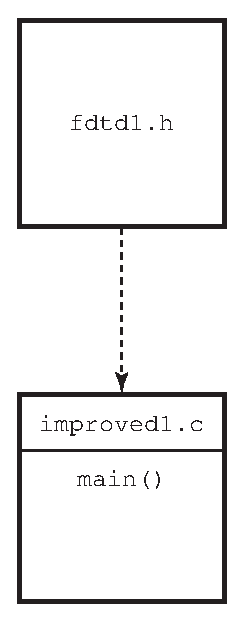
\epsfig{width=1.1in,file=Figures/Fdtd-improved-code/improved1-files.eps}
  \end{center} \caption{The files associated with the first improved
  version of the FDTD code.  The header file {\tt fdtd1.h} is included
  in the source file {\tt improved1.c} as indicated by the dashed
  line.  The source file {\tt improved1.c} contains the {\tt main()}
  function which performs all the executable statements associated with
  the simulation.}  \label{fig:improved1Files}
\end{figure}
The {\tt main()} function in file {\tt improved1.c} handles all the
calculations associated with the FDTD simulation.  Since there is only
a single source file, there is no obvious advantage to creating a
header file.  However, as we further modularize the code, the header
file will provide a convenient way to ensure that different source
files share common definitions of various things.  For example, many
source files may need to know about the details of a {\tt Grid}
structure.  These details can be written once in the header file and
then the header file can be included into different source files as
appropriate.  Examples of this will be provided in the following
sections.


\section{Modular Design and Initialization Functions\label{sec:modularDesign}}

Thus far all the programs have been written using a single source file
that contains a single function (the {\tt main()} function), or in the
case of the previous section, one source file and one header file.  As
the complexity of the FDTD simulation increases this approach becomes
increasingly unwieldy and error prone.  A better approach is to
modularize the program so that different functions perform specific
tasks---not everything is done within {\tt main()}.  For example, we
may want to use one function to update the magnetic field, another to
update the electric field, another to introduce energy into the grid,
and another to handle the termination of the grid.

Additionally, with C it is possible to put different functions in
different source files and compile the source files separately.  By
putting different functions in different source files, it is possible
to have different functions that are within one source file share
variables which are ``hidden'' from all functions that do not appear
in that file.  You can think of these variables as being private,
known only to the functions contained in the file.  As will be shown,
such sharing of variables can be useful when one wants to initialize
the behavior of a function that will be called multiple times (but the
initialization only needs to be done once).

To illustrate how functions within a file can share variables that are
otherwise hidden from other parts of a program, assume there is a
function that we want to call several times.  Further assume this
function performs a calculation based on some parameters but these
parameters only need to be set once---they will not vary from the
value to which they are initially set.  For this type of scenario, it
is often convenient to split the function into two functions: one
function handles the initialization of the parameters (the
``initialization function'') and the other function handles the
calculation based on those parameters (the ``calculation function'').
Now, the question is: How can the initialization function make the
parameters visible to the calculation function and how can the values
of these parameters persist between one invocation of the function and
the next?  The answer lies in global variables.

Generally the use of global variables is discouraged as they can make
programs hard to understand and difficult to debug.  However, global
variables can be quite useful when used properly.  To help minimize
the problems associated with global variables, we will further
modularizing the program so that the initialization function and
calculation function mentioned above are stored in a separate file
from the rest of the program.  In this way the global variables that
these functions share are not visible to any other function.

As a somewhat contrived example of this approach to setting
parameters, assume we want to write a program that will calculate the
values of a harmonic function where the user can specify the amplitude
and the phase, i.e., we want to calculate $f(x) = a\cos(x+\phi)$ where
$a$ is the amplitude and $\phi$ is the phase.  Note that we often just
write $f(x)$ for a function like this even though the function depends
on $a$ and $\phi$ as well as $x$.  We usually do {\em not} write
$f(x,a,\phi)$ because we think of $a$ and $\phi$ as fixed values (even
though they have to be specified at some point) while $x$ is the value
we are interested in varying.  Assume we want to write our program so
that there is a function {\tt harmonic1()} that is the equivalent of
$f(x) = a\cos(x+\phi)$.  {\tt harmonic1()} should take a single
argument that corresponds to the value of $x$.  We will use a separate
function, {\tt harmonicInit1()} that will set the amplitude and phase.

A file that contains a suitable the {\tt main()} function and the
associated statements to realize the parameter setting discussed above
is shown in Program \ref{pro:paramDemo1}.  The function prototypes for
{\tt harmonicInit1()} and {\tt harmonic1()} are given in lines
\ref{paramDemo1A} and \ref{paramDemo1B}, respectively.  Note, however,
that these functions do not appear in this file.  Between lines
\ref{paramDemo1C} and \ref{paramDemo1D} the user is prompted for the
amplitude and phase (and the phase is converted from degrees to
radians).  These values are passed as arguments to the {\tt
  harmonicInit1()} function.  As we will see a little later, this
function sets persistent global parameters to these values so that
they are visible to the function {\tt harmonic1()} whenever it is
called.  The for-loop that starts on line \ref{paramDemo1F} generates
the desired output values.  Here we set the variable {\tt x} to values
between $0$ and $2\pi$.  In line \ref{paramDemo1G} the value of {\tt x}
is printed together with the value of {\tt harmonic1(x)}.  Note that
the {\tt harmonic1()} function is not passed the amplitude or phase as
an argument.

\begin{program}
{\tt param-demo1.c}: File containing the {\tt main()} function and
appropriate header material that is used to demonstrate the setting of
persistent parameters in an auxilliary function.  Here {\tt
  harmonicInit1()} and {\tt harmonic1()} are serving this auxilliary
role.  The code associated with those functions is in a separate
file (see Program \ref{pro:harmonicDemo1}).
\label{pro:paramDemo1}
\codemiddle
\begin{lstlisting}
/* param-demo1.c:  Program that demonstrates the setting of
 * "persistent" parameters via the arguments of an initialization
 * function.  Here the parameters control the amplitude and phase of a
 * harmonic function f(x) = a cos(x + phi).  This program generates
 * num_points of the harmonic function with the "x" value of the
 * varying between zero and 2*pi.
 */

#include <stdio.h>
#include <math.h>  // To obtain M_PI, i.e., 3.14159...

void harmonicInit1(double amp, double phase);  /*@ \label{paramDemo1A} @*/
double harmonic1(double x);                    /*@ \label{paramDemo1B} @*/

int main() {
  double amp, phase, x;
  int mm, num_points = 100;

  printf("Enter the amplitude: ");       /*@ \label{paramDemo1C} @*/
  scanf(" %lf", &amp);
  printf("Enter the phase [in degrees]: ");
  scanf(" %lf", &phase);
  phase *= M_PI / 180.0;                 /*@ \label{paramDemo1D} @*/

  /* Set the amplitude and phase. */
  harmonicInit1(amp, phase);              /*@ \label{paramDemo1E} @*/

  for (mm = 0; mm < num_points; mm++) {   /*@ \label{paramDemo1F} @*/
    x = 2.0 * M_PI * mm / (float)(num_points - 1);
    printf("%f %f\n", x, harmonic1(x));  /*@ \label{paramDemo1G} @*/
  }

  return 0;
}
\end{lstlisting}
\end{program}

The file containing the functions {\tt harmonicInit1()} and {\tt
  harmonic1()} is shown in Program \ref{pro:harmonicDemo1}.  In line
\ref{paramDemo1A} two static double variables are declared: {\tt amp}
is the amplitude and {\tt phase} is the phase.  These variables are
visible to all the functions in this file but are not visible to any
other functions (despite the common name, these variables are distinct
from those with the same name in the {\tt main()} function).
Furthermore, the value of these variables will ``persist.''  They will
remain unchanged (unless we explicitly change them) and available for
our use through the duration of the running of the program.  (Note
that, it may perhaps be somewhat confusing, but the ``{\tt static}''
qualifier in line \ref{paramDemo1A} does not mean constant.  The value
of these variables can be changed.  Rather, it means these global
variables are local to this file.)

The {\tt harmonicInit1()} function starts on line \ref{harmonicDemo1B}.
It takes two arguments.  Here those arguments are labeled {\tt
  the\_amp} and {\tt the\_phase}.  We must distinguish these variable
names from the corresponding global variables.  We accomplish this by
putting the prefix {\tt the\_} on the corresponding global variable
name.  The global variables are set to the desired values in lines
\ref{harmonicDemo1C} and \ref{harmonicDemo1D}.  The {\tt harmonic1()}
function that begins on line \ref{harmonicDemo1E} then uses these
global values in the calculation of $a \cos(x+\phi)$.

\begin{program}
{\tt harmonic-demo1.c}: File containing the functions {\tt
  harmonicInit1()} and {\tt harmonic1()}.
\label{pro:harmonicDemo1}
\codemiddle
\begin{lstlisting}
/* 
 * harmonic-demo1.c: Functions to calculate a harmonic function of a
 * given amplitude and phase.  The desired amplitude and phase are
 * passed as arguments to harmonicInit1().  harmonicInit1() sets the
 * corresponding static global variables so that these values will be
 * available for the harmonic1() function to use whenever it is
 * called.
 */

#include <math.h> // for cos() function

/* Global static variables that are visible only to functions inside
   this file. */
static double amp, phase;     /*@ \label{harmonicDemo1A} @*/

// initialization function
void harmonicInit1(double the_amp, double the_phase) {  /*@ \label{harmonicDemo1B} @*/
  amp = the_amp;       /*@ \label{harmonicDemo1C} @*/
  phase = the_phase;   /*@ \label{harmonicDemo1D} @*/

  return;
}

// calculation function
double harmonic1(double x) {   /*@ \label{harmonicDemo1E} @*/
  return amp * cos(x + phase);
}
\end{lstlisting}
\end{program}

Now, let us change these programs in order to further separate the
{\tt main()} function from the harmonic function.  There is no reason
that the {\tt main()} function should have to prompt the user for the
amplitude or phase.  These values are simply passed along to the
harmonic initialization function and never actually used in {\tt
  main()}.  Thus, a better approach would be to let the harmonic
initialization function prompt the user for whatever input it needs.
The {\tt main()} function would merely call the initialization
function and leave all the details up to it.  So in the future, if one
wanted to change the harmonic function so the user could specify a
frequency as well as the amplitude and phase, that code could be added
to the harmonic functions but the {\tt main()} function would not have
to be changed in any way.

The new version of the {\tt main()} function is shown in Program
\ref{pro:paramDemo2}.  Note that there is now no mention of amplitude
or phase in {\tt main()}.  That information has all been relegated to
the harmonic functions themselves.

\begin{program}
  {\tt param-demo2.c}: Modified file containing the {\tt main()}
  function which demonstrates the use of an initialization function to
  set parameters.  In this version of the code the initilization
  function {\tt harmonicInit2()} takes no arguments.  The code for
  {\tt harmonicInit2()} and {\tt harmonic2()} is given in Program
  \ref{pro:harmonicDemo2}.
\label{pro:paramDemo2}
\codemiddle
\begin{lstlisting}
/* param-demo2.c: Program that demonstrates the setting of
 * "persistent" parameters via an initialization function.  Here the
 * initialization function handles all the details of obtaining the
 * parameters associated with the harmonic function.
 */

#include <stdio.h>
#include <math.h>  // To obtain M_PI, i.e., 3.14159...

void harmonicInit2();        /*@ \label{paramDemo2A} @*/
double harmonic2(double x);  /*@ \label{paramDemo2B} @*/

int main() {
  double x;
  int mm, num_points = 100;

  /* Initialize the harmonic function. */
  harmonicInit2();             /*@ \label{paramDemo2E} @*/

  for (mm = 0; mm < num_points; mm++) {   /*@ \label{paramDemo2F} @*/
    x = 2.0 * M_PI * mm / (float)(num_points - 1);
    printf("%f %f\n", x, harmonic2(x));  /*@ \label{paramDemo2G} @*/
  }

  return 0;
}
\end{lstlisting}
\end{program}

The file containing {\tt harmonicInit2()} and {\tt harmonic2()} is
shown in Program \ref{pro:harmonicDemo2}.  As before, the amplitude
and phase are global static variables that are declared in line
\ref{harmonicDemo2A}.  Note that {\tt harmonicInit2()} takes no
arguments.  Instead, this function prompts the user for the amplitude
and phase and sets the global variables appropriately.  Having done
this, these values are visible to the function {\tt harmonic2()}
(which is unchanged from the function {\tt harmonic1()} given
previously).

\begin{program}
{\tt harmonic-demo2.c}: File containing the functions {\tt
  harmonicInit2()} and {\tt harmonic2()}.
\label{pro:harmonicDemo2}
\codemiddle
\begin{lstlisting}
/* 
 * harmonic-demo2.c: Functions to calculate a harmonic function of a
 * given amplitude and phase.  harmonicInit2() prompts the user for
 * the amplitude and phase and sets the global variables so these
 * values will be available for the harmonic2() function to use
 * whenever it is called.
 */

#include <math.h> // for cos() function

/* Global static variables that are visible only to functions inside
   this file. */
static double amp, phase;     /*@ \label{harmonicDemo2A} @*/

// initialization function
void harmonicInit2() {  /*@ \label{harmonicDemo2B} @*/

  printf("Enter the amplitude: ");               /*@ \label{harmonicDemo2C} @*/
  scanf(" %lf", &amp);
  printf("Enter the phase [in degrees]: ");
  scanf(" %lf", &phase);
  phase *= M_PI / 180.0;                    /*@ \label{harmonicDemo2D} @*/

  return;
}

// calculation function
double harmonic2(double x) {   /*@ \label{harmonicDemo2E} @*/
  return amp * cos(x + phase);
}
\end{lstlisting}
\end{program}

In Sec.\ \ref{sec:compMultiFile} we will discuss the compilation of
multi-file programs such as these.


\section{Improvement Number Two}

Let us consider a further refinement to the simple bare-bones FDTD
simulation.  In this version of the code the updating of the electric
and magnetic fields will be handled by separate functions.  The grid
arrays will be initialized with a separate function and the source
function will be calculated using a separate function.  The
arrangement of the functions among the various files is depicted in
Fig.\ \ref{fig:improved2Files}.
\begin{figure}
  \begin{center}
  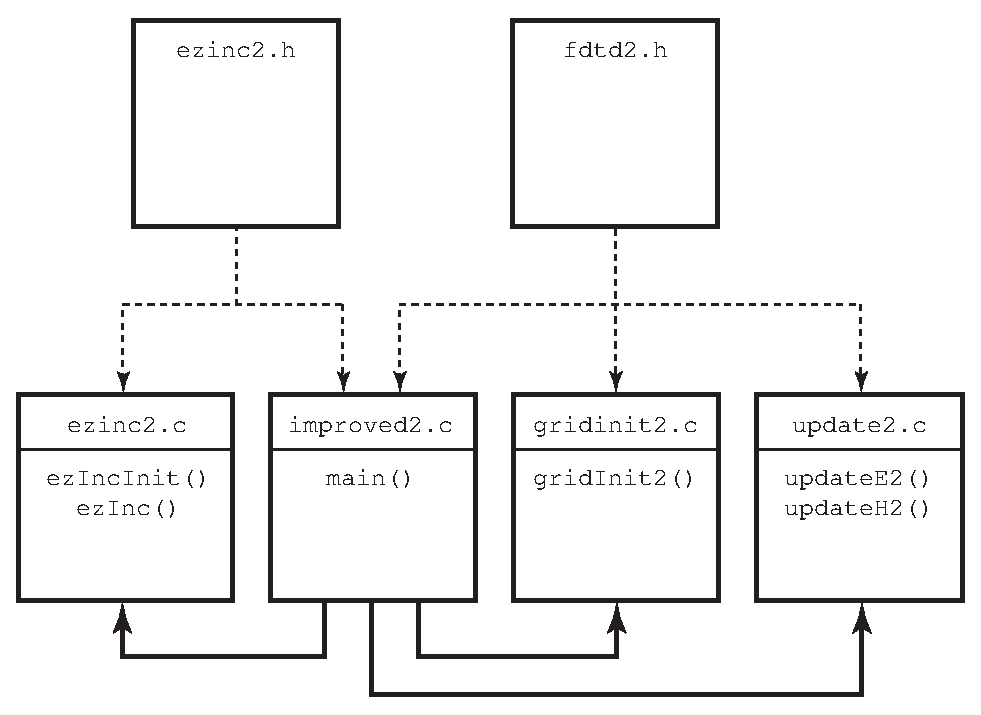
\epsfig{width=5.0in,file=Figures/Fdtd-improved-code/improved2-files.eps}
\end{center} \caption{The files associated with the second improved
  version of the FDTD code.  The header files {\tt fdtd2.h} and {\tt
    ezinc2.h} are included in the source files to which they are joined
  by a dashed line.  The file {\tt improved2.c} contains the {\tt
    main()} function but the initialization of the grid, the
  calculation of the source function, and the updating of the fields
  are no longer done in {\tt main()}.  Instead, other functions are
  called to accomplish these tasks.  The heavy black lines indicates
  which functions call which other functions.  In this case, {\tt
    main()} originates calls to all the other
  functions.}  \label{fig:improved2Files}
\end{figure}

Program \ref{pro:improved2} shows the contents of the file {\tt
  improved2.c}.  As indicated in Fig.\ \ref{fig:improved2Files}, {\tt
  main()} calls {\tt gridInit2()}.  This function initializes the {\tt
  Grid} structure {\tt g}.  The function {\tt gridInit2()} is
contained in the separate file {\tt gridinit2.c}.  The magnetic fields
are updated using the function {\tt updateH2()} while the electric
fields are updated using {\tt updateE2()}.  Both these functions are
contained in the file {\tt update2.c}.  The source function is
calculated using the function {\tt ezInc()} that is contained in the
file {\tt ezinc2.c}.

\begin{program} {\tt improved2.c}: Further code improvement of the
  bare-bones 1D FDTD simulation.  Here the initialization of the grid
  as well as the updating of the fields are handled by separate
  functions.  The argument for these functions is merely the {\tt
    Grid} pointer {\tt g}.  Additionally, the source function is
  initialized and calculated by separate
  functions. \label{pro:improved2} \codemiddle
\begin{lstlisting}
/* Version 2 of the improved bare-bones 1D FDTD simulation. */

#include "fdtd2.h"
#include "ezinc2.h"

int main()
{
  Grid *g;                             /*@ \label{improved2A} @*/

  ALLOC_1D(g, 1, Grid);       // allocate memory for Grid  /*@ \label{improved2B} @*/
  gridInit2(g);               // initialize the grid      /*@ \label{improved2C} @*/

  ezIncInit(g);               // initialize source function /*@ \label{improved2H} @*/

  /* do time stepping */
  for (Time = 0; Time < MaxTime; Time++) { /*@ \label{improved2D} @*/
    updateH2(g);              // update magnetic field  /*@ \label{improved2E} @*/
    updateE2(g);              // update electric field  /*@ \label{improved2F} @*/
    Ez(0) = ezInc(Time, 0.0); // apply source function  /*@ \label{improved2Z} @*/
    printf("%g\n", Ez(50));   // print output /*@ \label{improved2G} @*/
  } // end of time-stepping

  return 0;
}
\end{lstlisting}
\end{program}

Line \ref{improved2A} declares {\tt g} to be a pointer to a {\tt
  Grid}.  Since a {\tt Grid} structure has as elements the field
arrays, the time step, the duration of the simulations, and the
maximum number of time steps, none of these variables need to be
declared explicitly.  Note, however, that line \ref{improved2A} merely
creates a pointer but as yet this pointer does not point to anything
meaningful.  Line \ref{improved2B} uses {\tt ALLOC\_1D()} to allocated
memory for the {\tt Grid} and ensures {\tt g} points to that memory.
Assuming there were no errors in the allocation, this line is
effectively the equivalent of
\begin{code}
  g = calloc(1, sizeof(Grid));
\end{code}

As shown in lines \ref{improved2C}, \ref{improved2E}, and
\ref{improved2F}, {\tt gridInit2()}, {\tt updateH2()}, and {\tt
  updateE2()} each have a single argument: {\tt g} (a pointer to the
{\tt Grid}).  The parameters of the source function are initialized by
calling {\tt ezIncInit()} in line \ref{improved2H}.

The header file {\tt fdtd2.h} is shown in Program \ref{pro:fdtd2H}.
This file is largely the same as {\tt fdtd1.h}.  The only significant
difference is the function prototypes that are provided in lines
\ref{fdtd2HD}--\ref{fdtd2HF} for three of the functions called by {\tt
  main()} (note that the prototypes for the functions related to the
source are provided in {\tt ezinc2.h}).

\begin{program} {\tt fdtd2.h}: Header file to accompany the second
  version of the improved code showin in Program \ref{pro:improved2}.
  The differences between this file and {\tt fdtd1.h} are shown in
  bold. \label{pro:fdtd2H} \codemiddle
\begin{lstlisting}
/*b*/#ifndef _FDTD2_H
#define _FDTD2_H /*n*/

#include <stdio.h>
#include <stdlib.h>

struct Grid {
  double *ez;
  double *hy;
  int sizeX;
  int time, maxTime;
  double cdtds;
};

typedef struct Grid Grid;

/* memory allocation macro */
#define ALLOC_1D(PNTR, NUM, TYPE)                               \
    PNTR = (TYPE *)calloc(NUM, sizeof(TYPE));                   \
    if (!PNTR) {                                                \
      perror("ALLOC_1D");                                       \
      fprintf(stderr,                                           \
          "Allocation failed for " #PNTR ".  Terminating...\n");\
      exit(-1);                                                 \
    }

/* macros for accessing arrays and such */
#define Hy(MM)    g->hy[MM]
#define Ez(MM)    g->ez[MM]
#define SizeX     g->sizeX 
#define Time      g->time  
#define MaxTime   g->maxTime
#define Cdtds     g->cdtds

/*b*//* function prototypes */
void gridInit2(Grid *g);      /*@ \label{fdtd2HD} @*/
void updateH2(Grid *g);       /*@ \label{fdtd2HE} @*/
void updateE2(Grid *g);/*n*/  /*@ \label{fdtd2HF} @*/

#endif  /* matches #ifndef _FDTD2_H */
\end{lstlisting}
\end{program}

Program \ref{pro:update2} shows the contents of the file {\tt
  update2.c}.  The static global variable {\tt imp0} represents the
characteristic impedance of free space and is set to $377.0$ in line
\ref{update2A}.  This variable is never changed throughout the
program.  The magnetic field is updated with the function {\tt
  updateH2()} which is given between lines \ref{update2B} and
\ref{update2C}.  Note that the update equation uses {\tt Hy()} and
{\tt Ez()} to refer to the elements of the field arrays.  The macros
in {\tt fdtd2.h} translate these to the necessary syntax (which is
essentially {\tt g->hy[]} and {\tt g->ez[]}).  The electric field is
updated using {\tt updateE2()} which is given between lines
\ref{update2D} and \ref{update2F}.

\begin{program}
{\tt update2.c}: Source code for the functions {\tt updateH2()} and
{\tt updateE2()}. \label{pro:update2} 
\codemiddle
\begin{lstlisting}
/* Functions to update the electric and magnetic fields. */

#include "fdtd2.h"

/* characteristic impedance of free space */
static double imp0 = 377.0;  /*@ \label{update2A} @*/

/* update magnetic field */
void updateH2(Grid *g) {   /*@ \label{update2B} @*/
  int mm;

  for (mm = 0; mm < SizeX - 1; mm++)
    Hy(mm) = Hy(mm) + (Ez(mm + 1) - Ez(mm)) / imp0;

  return;
}                          /*@ \label{update2C} @*/

/* update electric field */
void updateE2(Grid *g) {   /*@ \label{update2D} @*/
  int mm;

  for (mm = 1; mm < SizeX - 1; mm++)
    Ez(mm) = Ez(mm) + (Hy(mm) - Hy(mm - 1)) * imp0;

  return;
}                          /*@ \label{update2F} @*/
\end{lstlisting}
\end{program}

Program \ref{pro:gridinit2} shows the source code for the function
{\tt gridInit2()}.  This function is used to set the value of various
elements of the {\tt Grid}.  (For this rather simple simulation, this
program is itself quite simple.)  Line \ref{gridinit2A} sets the size
of the Grid, {\tt SizeX}, to $200$.  Actually, after the preprocessor
has processed the code, this line will be
\begin{code}
  g->sizeX = 200;
\end{code}
Line \ref{gridinit2B} sets the duration of the simulation to $250$
time-steps.  Line \ref{gridinit2E} sets the Courant number to unity.
Lines \ref{gridinit2C} and \ref{gridinit2D} use the {\tt ALLOC\_1D()}
macro to allocate the necessary memory for the electric and magnetic
field arrays.

\begin{program}
{\tt gridinit2.c}: Source code for the function {\tt
gridInit2()}. \label{pro:gridinit2}
\codemiddle
\begin{lstlisting}
/* Function to initialize the Grid structure. */

#include "fdtd2.h"

void gridInit2(Grid *g) {
  SizeX = 200;                    // set the size of the grid /*@ \label{gridinit2A} @*/
  MaxTime = 250;                  // set duration of simulation /*@ \label{gridinit2B} @*/
  Cdtds = 1.0;                    // set Courant number /*@ \label{gridinit2E} @*/

  ALLOC_1D(g->ez, SizeX, double); // allocate memory for Ez /*@ \label{gridinit2C} @*/
  ALLOC_1D(g->hy, SizeX, double); // allocate memory for Hy /*@ \label{gridinit2D} @*/

  return;
}
\end{lstlisting}
\end{program}


Finally, Program \ref{pro:ezinc} shows the contents of the file {\tt
  ezinc2.c} which contains the code to implement the functions {\tt
  ezIncInit()} and {\tt ezInc()}.  The function {\tt ezinc()} is
Gaussian pulse whose width and delay are parameters that are set by
{\tt ezIncInit()}.  The implementation of this source function is
slightly different than in the original bare-bones code in that here
the user is prompted for the width and delay.  Additionally, the
source function {\tt ezInc()} takes two arguments, the time and the
location, so that this function can be used in a TFSF formulation.
When {\tt ezInc()} is called from {\tt main()}, the location is simply
hardwired to zero (ref.\ line \ref{improved2Z} of Program
\ref{pro:improved2}).

\begin{program} {\tt ezinc2.c}: File for the functions {\tt
    ezIncInit()} and {\tt ezInc()}.  {\tt ezInc()} is a traveling-wave
  implementation of a Gaussian pulse.  There are three private static
  global variables in this code.  These variables, representing the
  width and delay of the pulse as well as the Courant number, are
  determined and set by the initialization function {\tt ezIncInit()}.
  The Courant number is taken from the {\tt Grid} pointer that is
  passed as an argument while the user is prompted to provide the
  width and delay.
\label{pro:ezinc}
\codemiddle
\begin{lstlisting}
/* Functions to calculate the source function (i.e., the incident
 * field). */ 

#include "ezinc2.h"  /*@ \label{ezincY} @*/

/* global variables -- but private to this file */
static double delay, width = 0, cdtds;  /*@ \label{ezincX} @*/

/* prompt user for source-function width and delay. */
void ezIncInit(Grid *g){

  cdtds = Cdtds;  /*@ \label{ezincA} @*/
  printf("Enter delay: ");
  scanf(" %lf", &delay);
  printf("Enter width: ");
  scanf(" %lf", &width);

  return;
}

/* calculate source function at given time and location */
double ezInc(double time, double location) {
  if (width <= 0) {
    fprintf(stderr,
       "ezInc: must call ezIncInit before ezInc.\n"
       "       Width must be positive.\n");
    exit(-1);
  }
  return exp(-pow((time - delay - location / cdtds) / width, 2));
}
\end{lstlisting}
\end{program}

In Program \ref{pro:ezinc} the variable {\tt width} is used to
determine if initialization has been done.  {\tt width} is initialized
to zero when it is declared in line \ref{ezincX}.  If it is not
positive when {\tt ezInc()} is called, an error message is printed and
the program terminates.  In practice one should check that all the
parameters have been set to reasonable values, but here we only check
the width.

The private variable {\tt cdtds} declared in line \ref{ezincX} is
distinct from {\tt Cdtds} which the preprocessor expands to {\tt
  g->cdtds}.  That is to say the Courant number {\tt cdtds} that is an
element within the {\tt Grid} is different from the private variable
{\tt cdtds} in this file.  But, of course, we want these values to be
the same and line \ref{ezincA} assures this.

The header file to accompany {\tt ezinc2.c} is shown in Program {\tt
  ezinc2.h}.  As well as providing the necessary function prototypes,
this file ensures the inclusion of {\tt fdtd2.h} (which provides the
description a {\tt Grid} structure).

\begin{program}
{\tt ezinc2.h}: Header file that accompanies {\tt ezinc2.c} and is also
included in the file that specifies {\tt main()} (i.e., the file {\tt
  improved2.c}.
\label{pro:ezincH} 
\codemiddle
\begin{lstlisting}
/* Header file to accompany ezinc2.c. */

#ifndef _EZINC2_H   /*@ \label{ezincHA} @*/
#define _EZINC2_H   /*@ \label{ezincHB} @*/

#include <math.h>
#include <stdio.h>
#include <stdlib.h>
#include "fdtd2.h"   /*@ \label{ezincHC} @*/

void ezIncInit(Grid *g);
double ezInc(double time, double location);

#endif  /* matches #ifndef _EZINC2_H */          /*@ \label{ezincHD} @*/
\end{lstlisting}
\end{program}

\section{Compiling Modular Code \label{sec:compMultiFile}}

When a program is divided between multiple files it is typically not
necessary to recompile every file if there was a change in only some
of them.  Each source file can be compiled individually to an ``object
file'' or object code.  An object file, by itself, is not executable.
(To create executable code, all the object code must be linked
together.)  To create an object file with the GNU C compiler, one uses
the {\tt -c} flag.  Thus, for example, to obtain the object file for
{\tt ezinc2.c}, one would issue a command such as \index{gcc!object
  code}
\begin{code}
  gcc -Wall -O -c ezinc2.c
\end{code}
The flag {\tt -Wall} means to show all warnings, while {\tt -O} tells
the compiler to optimize the code (greater optimization can be
obtained by instead using {\tt -O2} or {\tt -O3}---the greater
optimization usually comes at the cost of slower compilation and larger
object and executable files).  When this command is issued the
compiler will create the object file {\tt ezinc2.o}.

The object files for all the components of the program can be created
separately by reissuing commands similar to the one shown above,
e.g., 
\begin{code}
  gcc -Wall -O -c ezinc2.c
  gcc -Wall -O -c improved2.c
  gcc -Wall -O -c update2.c
  gcc -Wall -O -c gridinit2.c
\end{code}
These commands would create the object files {\tt ezinc2.o}, {\tt
improved2.o}, {\tt update2.o}, and {\tt gridinit2.o}.  Alternatively,
one can create all the object files at once using a command such as
\begin{code}
  gcc -Wall -O -c ezinc2.c improved2.c update2.c gridinit2.c
\end{code}

\index{gcc!linking}
No matter how the object files are created, they need to be linked
together to obtain an executable.  The command to accomplish this is
\begin{code}
  gcc ezinc2.o improved2.o update2.o gridinit2.o -lm -o improved2
\end{code}
The flag {\tt -lm} tells the compiler to link to the math library
(which is necessary because of the math functions used in {\tt
ezinc2.c}).  The {\tt -o} flag allows one to specify the name of the
output/executable file, in this case {\tt improved2}.

For small programs there is not much advantage to incremental
compilation.  However, as the software increases in size and
complexity, there may be a significant savings in time realized by
recompiling only the code that has changed.  For example, assume a
change was made in the file {\tt gridinit2.c} but in no other.  Also
assume that the object code for each file has previously been created.
To obtain an executable that reflects this change one merely needs to
recompile this one file and then link the resulting object file to the
others, i.e.,
\begin{code}
  gcc -Wall -O -c gridinit2.c
  gcc ezinc2.o improved2.o update2.o gridinit2.o -lm -o improved2
\end{code}

\index{make}\index{makedepend} The details of incremental compilations
can actually be handled by utilities that detect the files that need
to be recompiled and react accordingly.  Those who are interested in
an example of such a utility may be interested in the {\tt make}
utility which is available on most Unix-based machines.  Another
helpful utility, which goes hand-in-hand with {\tt make} is {\tt
  makedepend} which sorts out the dependence of all the source files
on the header files.  {\tt make} is a rather old utility---going back
to the early days of Unix---and there are alternatives available such
as SCons available from \url{www.scons.org}.

\section{Improvement Number Three \label{sec:improveThree}}

Now let us modularize the program that contained the matched lossy
layer (Program \ref{pro:1Dmatched}).  As shown in Fig.\
\ref{fig:improvedFiles}, we will use separate functions for
initializing the grid, taking snapshots, applying the TFSF boundary,
updating the grid, and applying the ABC.  Additionally, the
calculation of the incident source function will be handled by a
separate function.  This source function will be called by the
function that implements the TFSF boundary, but no other.  Each box in
Fig.\ \ref{fig:improvedFiles} represents a separate file that contains
one or more functions.  The dashed lines indicate the inclusion of
header files and the heavy lines indicate function calls from one file
to another.

\begin{figure}
  \begin{center}
  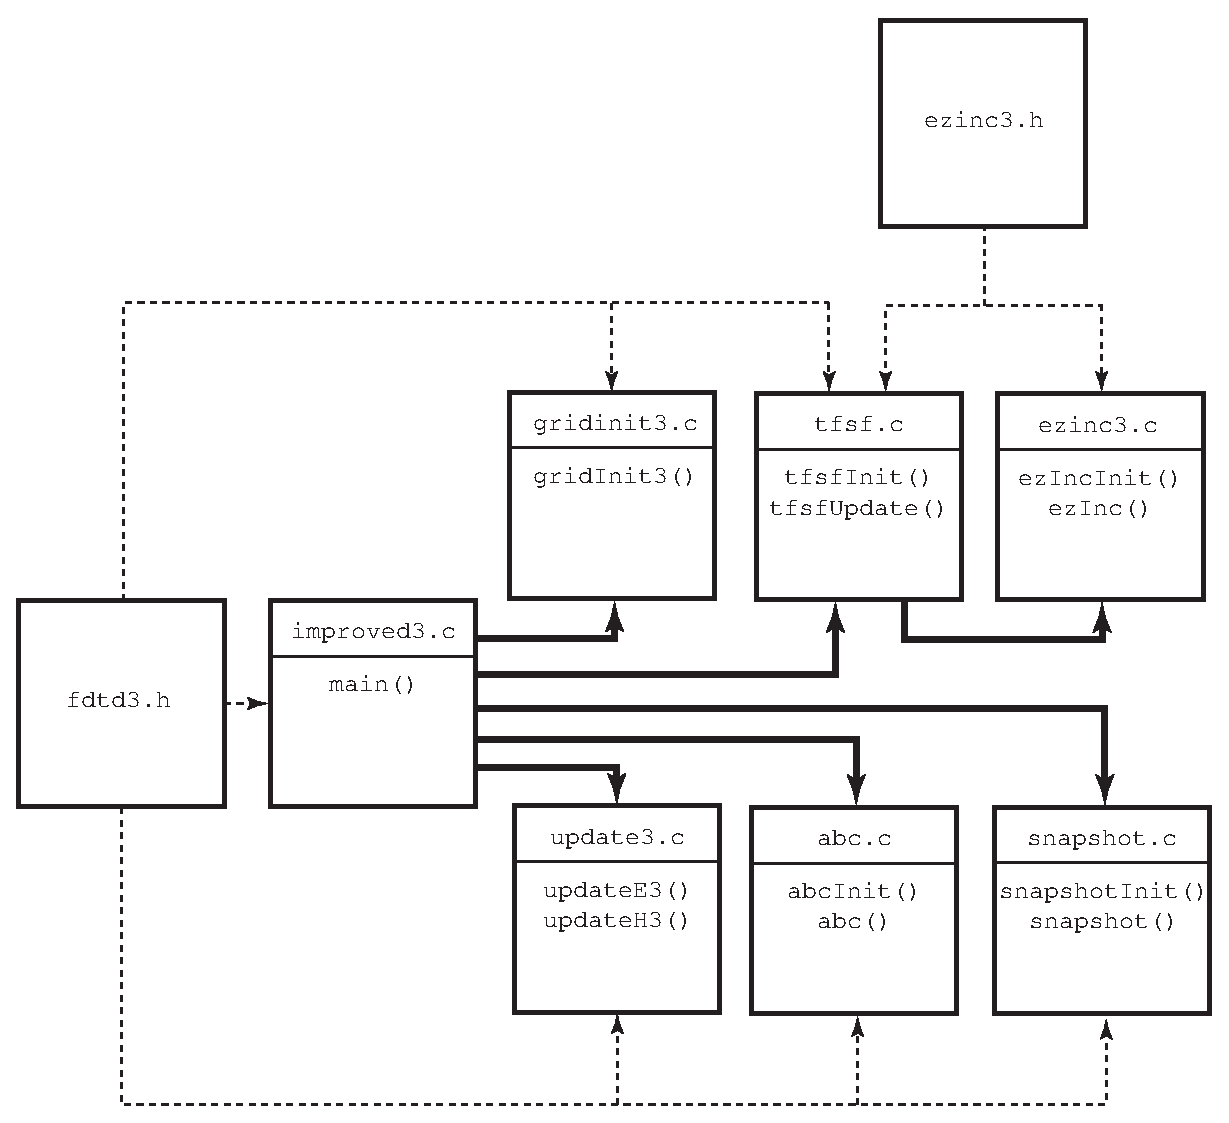
\epsfig{width=6.3in,file=Figures/Fdtd-improved-code/improved3-files.eps}
  \end{center} \caption{The files associated with the third
  improvement of the FDTD code.  The header file {\tt fdtd3.h} is
  explicitly included in the source files to which it is joined by a
  dashed line.  (Wherever {\tt ezinc3.h} appears it also ensures {\tt
  fdtd3.h} is included.)  The file {\tt improved3.c} contains the
  {\tt main()} function but the initialization of the grid, the
  application of the absorbing boundary condition, the calculation of
  the source function, the updating of the fields, and the taking of
  the snapshots is no longer done in {\tt main()}.  Instead, other
  functions are called to accomplish these tasks.}
  \label{fig:improvedFiles}
\end{figure}

The source code {\tt improved3.c} which contains the {\tt main()}
function is shown in Program \ref{pro:improved3}.  Note that nearly
all activities associated with the FDTD simulation are now done by
separate functions.  {\tt main()} merely serves to ensure that proper
initialization is done and then implements the time-stepping loop in
which the various functions are called.

\begin{program}
{\tt improved3.c}: Source code containing the {\tt main()} function.
Nearly all the FDTD related activities have been relegated to separate
functions which are called from {\tt main()}.  \label{pro:improved3}
\codemiddle
\begin{lstlisting}
/* FDTD simulation where main() is primarily used to call other
 * functions that perform the necessary operations. */

#include "fdtd3.h"

int main()
{
  Grid *g;

  ALLOC_1D(g, 1, Grid);  // allocate memory for Grid

  gridInit3(g);        // initialize the grid  /*@ \label{improved3A} @*/
  abcInit(g);          // initialize ABC       /*@ \label{improved3C} @*/
  tfsfInit(g);         // initialize TFSF boundary
  snapshotInit(g);     // initialize snapshots /*@ \label{improved3B} @*/

  /* do time stepping */
  for (Time = 0; Time < MaxTime; Time++) {
    updateH3(g);   // update magnetic field
    tfsfUpdate(g); // correct field on TFSF boundary
    abc(g);        // apply ABC
    updateE3(g);   // update electric field
    snapshot(g);   // take a snapshot (if appropriate)
  } // end of time-stepping

  return 0;
}
\end{lstlisting}
\end{program}

We have any number of options in terms of how functions should be
initialized or what arguments they should be passed.  Thus, one should
not consider this code to be optimum in any way.  Rather this code is
being used to illustrate implementation options.  

As in the previous program, {\tt main()} starts by defining a {\tt
  Grid} pointer and allocating space for the actual structure.  Then,
in lines \ref{improved3A}--\ref{improved3B}, four initialization
functions are called.  {\tt gridInit3()} initializes the {\tt Grid}
(this will be discussed in more detail shortly).  {\tt abcInit()}
handles any initialization associated with the ABC (as we will see, in
this particular case there is nothing for this initialization function
to do).  {\tt tfsfInit()} initializes the TFSF boundary while {\tt
  snapshotInit()} does the necessary snapshot initialization.
Following these initialization steps is the time-stepping loop where
the various functions are called that do the actual calculations.

The header {\tt fdtd3.h} is shown in Program \ref{pro:fdtd3h}.
Looking just at {\tt improved3.c} you would be unaware that the {\tt
  Grid} structure has changed.  However, four pointers have been added
that will contain the update-equation coefficients.  As can be seen in
lines \ref{fdtd3hA} and \ref{fdtd3hB} of Program \ref{pro:fdtd3h},
these pointers are named {\tt ceze}, {\tt cezh}, {\tt chyh}, and {\tt
  chye}.  Besides this and besides providing the function prototypes
for the new functions, this header file is largely the same as {\tt
  fdtd2.h}.
\begin{program}
{\tt fdtd3.h}: Header file to accompany {\tt improved3.c}.
Differences from {\tt fdtd2.h} are shown in bold.  \label{pro:fdtd3h}
\codemiddle
\begin{lstlisting}
/*b*/#ifndef _FDTD3_H
#define _FDTD3_H /*n*/

#include <stdio.h>
#include <stdlib.h>

struct Grid {
  double *ez, /*b*/*ceze, *cezh;/*n*/ /*@ \label{fdtd3hA} @*/
  double *hy, /*b*/*chyh, *chye;/*n*/ /*@ \label{fdtd3hB} @*/
  int sizeX;
  int time, maxTime;
  double cdtds;
};

typedef struct Grid Grid;

/* macros for accessing arrays and such */
#define Hy(MM)    g->hy[MM]
/*b*/#define Chyh(MM)  g->chyh[MM]
#define Chye(MM)  g->chye[MM]  /*n*/

#define Ez(MM)    g->ez[MM]
/*b*/#define Ceze(MM)  g->ceze[MM]
#define Cezh(MM)  g->cezh[MM]  /*n*/

#define SizeX     g->sizeX
#define Time      g->time
#define MaxTime   g->maxTime
#define Cdtds     g->cdtds

/* memory allocation macro */
#define ALLOC_1D(PNTR, NUM, TYPE)                               \
    PNTR = (TYPE *)calloc(NUM, sizeof(TYPE));                   \
    if (!PNTR) {                                                \
      perror("ALLOC_1D");                                       \
      fprintf(stderr,                                           \
          "Allocation failed for " #PNTR ".  Terminating...\n");\
      exit(-1);                                                 \
    }

/* Function prototypes */ /*b*/
void abcInit(Grid *g);
void abc(Grid *g);

void gridInit3(Grid *g);

void snapshotInit(Grid *g);
void snapshot(Grid *g);

void tfsfInit(Grid *g);
void tfsfUpdate(Grid *g);

void updateE3(Grid *g);
void updateH3(Grid *g); /*n*/

#endif  /* matches #ifndef _FDTD3_H */
\end{lstlisting}
\end{program}

The function {\tt gridInit3()} is contained in the file {\tt
  gridinit3.c} shown in Program \ref{pro:gridinit3}.  Keep in mind
that it does not matter what file names are---file names do not have
to match the contents of the file in any way, but, of course, it is
best to use names that are descriptive of the contents.

The preprocessor directives in lines
\ref{gridinit3A}--\ref{gridinit3B} are simply to provide convenient
names to the amount of loss, the starting location of the lossy layer,
and the relatively permittivity of the half space.  These parameters
are the same as they were in Program \ref{pro:1Dmatched}.

\begin{program} {\tt gridinit3.c}: The {\tt gridInit3()} function to
  initialize the {\tt Grid}.
\label{pro:gridinit3}
\codemiddle
\begin{lstlisting}
/* Function initialize Grid structure. */

#include "fdtd3.h"

#define LOSS 0.02       /*@ \label{gridinit3A} @*/
#define LOSS_LAYER 180  // node at which lossy layer starts
#define EPSR 9.0        /*@ \label{gridinit3B} @*/

void gridInit3(Grid *g) {
  double imp0 = 377.0;
  int mm;

  SizeX = 200;   // size of domain         /*@ \label{gridinit3C} @*/
  MaxTime = 450; // duration of simulation
  Cdtds = 1.0;   // Courant number         /*@ \label{gridinit3D} @*/

  ALLOC_1D(g->ez,   SizeX, double);  /*@ \label{gridinit3E} @*/
  ALLOC_1D(g->ceze, SizeX, double);
  ALLOC_1D(g->cezh, SizeX, double);
  ALLOC_1D(g->hy,   SizeX - 1, double);
  ALLOC_1D(g->chyh, SizeX - 1, double);
  ALLOC_1D(g->chye, SizeX - 1, double);  /*@ \label{gridinit3F} @*/
  
  /* set electric-field update coefficients */
  for (mm = 0; mm < SizeX; mm++)
    if (mm < 100) {
      Ceze(mm) = 1.0;
      Cezh(mm) = imp0;
    } else if (mm < LOSS_LAYER) {
      Ceze(mm) = 1.0;
      Cezh(mm) = imp0 / EPSR;
    } else {
      Ceze(mm) = (1.0 - LOSS) / (1.0 + LOSS);
      Cezh(mm) = imp0 / EPSR / (1.0 + LOSS);
    }

  /* set magnetic-field update coefficients */
  for (mm = 0; mm < SizeX - 1; mm++)
    if (mm < LOSS_LAYER) {
      Chyh(mm) = 1.0;
      Chye(mm) = 1.0 / imp0;
    } else {
      Chyh(mm) = (1.0 - LOSS) / (1.0 + LOSS);
      Chye(mm) = 1.0 / imp0 / (1.0 + LOSS);
    }

  return;
}
\end{lstlisting}
\end{program}

Lines \ref{gridinit3C}--\ref{gridinit3D} set the size of the {\tt
  Grid}, the duration of the simulation, and the Courant number.
Lines \ref{gridinit3E}--\ref{gridinit3F} allocate the necessary memory
for the various arrays.  The coefficient arrays are then set as they
were in Program \ref{pro:1Dmatched}.

The functions to update the electric and magnetic fields, i.e., {\tt
  updateE3()} and {\tt updateH3()} are contained in the file {\tt
  update3.c}.  The contents of this file are shown in Program
\ref{pro:update3}.  The functions are largely unchanged from those
that appeared in Program \ref{pro:update2}.  The only significant
differences are the appearance of the coefficient arrays in the update
equations that start on lines \ref{update3A} and \ref{update3B}.
\begin{program}
{\tt update3.c}: Functions to update the electric and magnetic fields.
\label{pro:update3}
\codemiddle
\begin{lstlisting}
/* Functions to update the electric and magnetic fields. */

#include "fdtd3.h"

/* update magnetic field */
void updateH3(Grid *g) {
  int mm;

  for (mm = 0; mm < SizeX - 1; mm++)
    Hy(mm) = Chyh(mm) * Hy(mm) +          /*@ \label{update3A} @*/
             Chye(mm) * (Ez(mm + 1) - Ez(mm));

  return;
}

/* update electric field */
void updateE3(Grid *g) {
  int mm;

  for (mm = 1; mm < SizeX - 1; mm++)
    Ez(mm) = Ceze(mm) * Ez(mm) +      /*@ \label{update3B} @*/
             Cezh(mm) * (Hy(mm) - Hy(mm - 1));

  return;
}
\end{lstlisting}
\end{program}

The function to apply the absorbing boundary conditions is rather
trivial and is shown in Program \ref{pro:abcTrivial}.  Also shown in
Program \ref{pro:abcTrivial} is the initiliztaion function {\tt
  abcInit()}.  In this particular case the ABC is so simple that there
is no initializataion that needs to be done and hence this function
simply returns.  In Chap.\ \ref{chap:abc} we will begin to consider more
sophisticated ABC's that do indeed require some initialization.  Thus,
this call the initialization function is done in anticipation of that.
As was the case in Program \ref{pro:1Dmatched}, the ABC is only
applied to the left side of the grid.  The right side of the grid is
terminated with a lossy layer.

\begin{program}
{\tt abc.c}: Absorbing boundary condition used by {\tt improved3.c}.
For this particular simple ABC there is nothing for the initialization
function to do and hence it simply returns.
\label{pro:abcTrivial}
\codemiddle
\begin{lstlisting}
/* Functions to terminate left side of grid. */

#include "fdtd3.h"

// Initialize the ABC -- in this case, there is nothing to do.
void abcInit(Grid *g) {

  return;
}

// Apply the ABC -- in this case, only to the left side of grid.
void abc(Grid *g) {

  /* simple ABC for left side of grid */
  Ez(0) = Ez(1);

  return;
}
\end{lstlisting}
\end{program}

The code associated with the TFSF boundary is shown in Program
\ref{pro:tfsfTrivial}.  Line \ref{tfsfTrivA} declares a static global
variable {\tt tfsfBoundary} which specifies the location of the TFSF
boundary.  This variable is initialized to zero with the understanding
that when the code is initialized it will be set to some meaningful
(positive) value.

\begin{program}
{\tt tfsf.c}: Code to implement the TFSF boundary.
\label{pro:tfsfTrivial}
\codemiddle
\begin{lstlisting}
/* Function to implement a 1D FDTD boundary. */

#include <math.h>
#include "fdtd3.h"
#include "ezinc3.h"

static int tfsfBoundary = 0;  /*@ \label{tfsfTrivA} @*/

void tfsfInit(Grid *g) {    /*@ \label{tfsfTrivB} @*/

  printf("Enter location of TFSF boundary: ");
  scanf(" %d", &tfsfBoundary);

  ezIncInit(g); // initialize source function /*@ \label{tfsfTrivD} @*/

  return;
}

void tfsfUpdate(Grid *g) {   /*@ \label{tfsfTrivE} @*/
  /* check if tfsfInit() has been called */
  if (tfsfBoundary <= 0) {
    fprintf(stderr,
      "tfsfUpdate: tfsfInit must be called before tfsfUpdate.\n"
      "            Boundary location must be set to positive value.\n");
    exit(-1);
  }

  /* correct Hy adjacent to TFSF boundary */
  Hy(tfsfBoundary) -= ezInc(Time, 0.0) * Chye(tfsfBoundary);
    
  /* correct Ez adjacent to TFSF boundary */
  Ez(tfsfBoundary + 1) += ezInc(Time + 0.5, -0.5);
  
  return;
}
\end{lstlisting}
\end{program}

The initialization function {\tt tfsfInit()} begins on line
\ref{tfsfTrivB}.  The user is prompted to enter the location of the
TFSF boundary.  Then the initialization function for the source {\tt
  ezIncInit()} is called to set the parameters that control the shape
of the pulse.  

The code to calculate the source function, i.e., the functions {\tt
  ezIncInit()} and {\tt ezInc()} is identical to that shown in Program
\ref{pro:ezinc}.  However, there would be one slight change to the
file: instead of including {\tt ezinc2.h}, line \ref{ezincY} of
Program \ref{pro:ezinc} would be changed to include {\tt ezinc3.h}.
We assume this modified program is in the file {\tt ezinc3.c} which is
not shown.  The header file {\tt ezinc3.h} would be nearly identical
to the code shown in Program \ref{pro:ezincH} except the ``$2$'' in
lines \ref{ezincHA}, \ref{ezincHB}, and \ref{ezincHC}, would be
changed to ``$3$'' (thus ensuring the proper inclusion of the header
file {\tt fdtd3.h} instead of {\tt fdtd2.h}).  Again, since this is
such a minor change, the contents of {\tt ezinc3.h} are not shown.

The function {\tt tfsfUpdate()} which begins on line \ref{tfsfTrivE}
is called once every time-step.  This function applies the necessary
correction to the nodes adjacent to the TFSF boundary.  Because of the
implicit timing within this file, this function needs to be called
after the magnetic-field update, but before the electric-field update.
The function first checks that the boundary location is positive.  If
it is not, an error message is printed and the program terminates,
otherwise the fields adjacent to the boundary are corrected.

Finally, the code associated with taking snapshots of the field is
shown in Program \ref{pro:snapTrivial}.  {\tt snapshotInit()} allows
the user to specify the time at which snapshots should start, the
temporal stride between snapshots, the node at which a snapshot should
start, the node at which it should end, the spatial stride between
nodes, and the base name of the output files.  Assuming the user
entered a base name of {\tt sim}, then, as before, the output files
would be named {\tt sim.0}, {\tt sim.1}, {\tt sim.2}, and so on.  If
the user said the {\tt startTime} is $105$ and the {\tt
temporalStride} is $10$, then snapshots would be taken at time-steps
$105$, $115$, $125$, and so on.  Similarly, if the user specified that
the {\tt startNode} and {\tt endNode} are $0$ and $180$, respectively,
and the {\tt spatialStride} is $1$, then the value of every node
between $0$ and $180$, inclusive, would be recorded to the snapshot
file.  If the {\tt spatialStride} were $2$, every other node would be
recorded.  If it were $3$, every third node would be recorded.
(Because of this, the {\tt endNode} only corresponds to the actual
last node in the snapshot file if its offset from the {\tt startNode}
is an even multiple of the spatial stride.)

\begin{program}
{\tt snapshot.c}: Code for taking snapshots of the electric field.
\label{pro:snapTrivial}
\codemiddle
\begin{lstlisting}
/* Function to take a snapshot of a 1D grid. */

#include "fdtd3.h"

static int temporalStride = 0, spatialStride, startTime,
  startNode, endNode, frame = 0;
static char basename[80];

void snapshotInit(Grid *g) { /*@ \label{snapTrivA} @*/
  
  printf("For the snapshots:\n");
  printf("  Duration of simulation is %d steps.\n", MaxTime);
  printf("  Enter start time and temporal stride: ");
  scanf(" %d %d", &startTime, &temporalStride);
  printf("  Grid has %d total nodes (ranging from 0 to %d).\n",
	 SizeX, SizeX-1);
  printf("  Enter first node, last node, and spatial stride: ");
  scanf(" %d %d %d", &startNode, &endNode, &spatialStride);
  printf("  Enter the base name: ");
  scanf(" %s", basename);

  return;
}

void snapshot(Grid *g) { /*@ \label{snapTrivB} @*/
  int mm;
  char filename[100];
  FILE *snapshot;

  /* ensure temporal stride set to a reasonable value */
  if (temporalStride <= 0) {
    fprintf(stderr,
      "snapshot: snapshotInit must be called before snapshot.\n"
      "          Temporal stride must be set to positive value.\n");
    exit(-1);
  }

  /* get snapshot if temporal conditions met */
  if (Time >= startTime && 
      (Time - startTime) % temporalStride == 0) {
    sprintf(filename, "%s.%d", basename, frame++);
    snapshot = fopen(filename, "w");
    for (mm = startNode; mm <= endNode; mm += spatialStride)
      fprintf(snapshot, "%g\n", Ez(mm));
    fclose(snapshot);
  }

  return;
}
\end{lstlisting}
\end{program}

As shown in line \ref{snapTrivA}, {\tt snapshotInit()} takes a single
argument, a pointer to a {\tt Grid} structure.  This function prompts
the user to set the appropriate snapshot control values.  The snapshot
files themselves are created by the function {\tt snapshot()} which
starts on line \ref{snapTrivB}.  This function starts by checking that
the temporal stride has been set to a reasonable value.  If not, an
error message is printed and the program terminates.  The program then
checks if time is greater than or equal to {\tt startTime} and the
difference between the current time and the {\tt startTime} is a
multiple of {\tt temporalStride}.  If not, the function returns.  If
those conditions are met, then, as we have seen before, a snapshot
file is written and the frame counter is advanced.  However, now there
is some control over which nodes are actually written.  Note that the
function {\tt snapshot()} is called every time-step.  We could easily
have checked in the {\tt main()} function if the time-step was such
that a snapshot should be generated and only then called {\tt
  snapshot()}.  Reasons for adopting either approach could be made but
be aware that the overhead for calling a function is typically small.
Thus, the savings realized by calling {\tt snapshot()} less often (but
still ultimately generating the same number of snapshots) is likely to
be trivial.  The approach used here keeps all the snapshot-related
data in the snapshot code itself.

After compiling all this code (and linking it), the executable will
produce the same results as were obtained from Program
\ref{pro:1Dmatched} (assuming, of course, the user enters the same
parameters as were used in Program \ref{pro:1Dmatched}).  With the new
version of the code there are several improvements we could
potentially use to our advantage.  Assume, for instance, we wanted to
do simulations of two different scenarios.  We could create two {\tt
  Grid} structures, one for scenario.  Each grid would have its own
{\tt gridInit()} function, but other than that all the code could be
used by either grid.  The update functions could be applied, without
any modification, to any grid.  The snapshot function could be applied
to any grid, and so on.



\chapter{Scaling FDTD Simulations to Any Frequency
 \label{chap:dimensionless}}

%\setcounter{page}{1}

\renewcommand{\thefootnote}{\fnsymbol{footnote}}
\footnotetext{Lecture notes by John Schneider.  {\tt
fdtd-dimensionless.tex}}

\section{Introduction}

The FDTD method requires the discretization of time and space.
Samples in time are $\Delt$ apart whereas, in simulations with one
spatial dimension, samples in space are $\Delx$ apart.  It thus
appears that one must specify $\Delt$ and $\Delx$ in order to perform
a simulation.  However, as shown in Sec.\ \ref{sec:update}, it is
possible to write the coefficients $\Delt/\epsilon\Delx$ and
$\Delt/\mu\Delx$ in terms of the material parameters and the Courant
number (ref.\ \refeq{eq:coefEz} and \refeq{eq:coefHy}).  Since the
Courant number contains the ratio of the temporal step to the spatial
step, it allows one to avoid explicitly stating a definite temporal or
spatial step---all that matters is their ratio.  This chapter
continues to examine ways in which FDTD simulations can be treated as
generic simulations that can be scaled to any size/frequency.  As will
be shown, the important factors which dictate the behavior of the
fields in a simulation are the Courant number and the points per
wavelength for any given frequency.  We conclude the chapter by
considering how one can obtain the transmission coefficient for a
planar interface from a FDTD simulation.

\section{Sources}

\subsection{Gaussian Pulse}

In the previous chapter the source function, whether hardwired,
additive, or incorporated in a TFSF formulation, was always a
Gaussian.  In the continuous world this function can be expressed as
\begin{equation}
  f_g(t) = e^{-\left(\frac{t - d_g}{w_g}\right)^2}
  \label{eq:gaussianGeneric}
\end{equation}
where $d_g$ is the temporal delay and $w_g$ is a pulse-width
parameter.  The Gaussian has its peak value at $t=d_g$ (when the
exponent is zero) and has a value of $e^{-1}$ when $t=d_g\pm w_g$.
Since \refeq{eq:gaussianGeneric} is only a function of time, i.e., a
function of $q\Delt$ in the discretized world, it again appears as if
the temporal step $\Delt$ must be given explicitly.  However, if one
specifies the delay and pulse width in terms of temporal steps, the
term $\Delt$ appears in both the numerator and the denominator of the
exponent.  For example, in the last chapter $d_g$ was $30\Delt$ and
$w_g$ was $10\Delt$ so the source function could be written
\begin{equation}
   f_g(q\Delt) = f_g[q] = e^{-\left(\frac{q - 30}{10}\right)^2}.
\end{equation}
Note that $\Delt$ does not appear on the right-hand side.  

The discretized version of a function $f(q\Delt)$ will be written
$f[q]$, i.e., the temporal step will be dropped from the argument
since it does not appear explicitly in the expression for the function
itself.  The key to being able to discard $\Delt$ from the source
function was the fact that the source parameters were expressed in
terms of the number of temporal steps.

\subsection{Harmonic Sources \label{sec:harmonicSources}}

For a harmonic source, such as
\begin{equation}
  f_h(t)=\cos(\omega t),
\end{equation}
there is no explicit numerator and denominator in the argument.
Replacing $t$ with $q\Delt$ it again appears as if the temporal step
must be given explicitly.  However, keep in mind that with
electromagnetic fields there is an explicit relationship between
frequency and wavelength.  For a plane wave propagating in free space,
the wavelength $\lambda$ and frequency $f$ are related by
\begin{equation}
  f \lambda=c \qquad\Rightarrow \qquad f=\frac{c}{\lambda}.
\end{equation}
Thus the argument $\omega t$ (i.e., $2 \pi f t$) can also be written
as
\begin{equation}
  \omega t = \frac{2\pi c}{\lambda}t.
\end{equation}
For a given frequency, the wavelength is a fixed length.  Being a
length, it can be expressed in terms of the spatial step, i.e.,
\begin{equation}
  \lambda = \ppw \Delx
\end{equation}
where $\ppw$ is the number of points per wavelength.  This does not
need to be an integer.

By relating frequency to wavelength and the wavelength to $\ppw$, the
discretized version of the harmonic function can be written
\begin{equation}
 f_h(q\Delt) = \cos\!\left(\frac{2 \pi c}{\ppw\Delx} q \Delt\right)
           = \cos\!\left(\frac{2 \pi}{\ppw}\frac{c\Delt}{\Delx} q\right),
 \label{eq:fHarmonic}
\end{equation}
or, simply,
\begin{equation}
   f_h[q] = \cos\!\left(\frac{2 \pi S_c}{\ppw} q\right).
 \label{eq:fHarmonicI}
\end{equation}
The expression on the right now contains the Courant number and the
parameter $\ppw$.  In this form one does not need to state an explicit
value for the temporal step.  Rather, one specifies the Courant
number $S_c$ and the number of spatial steps per wavelength $\ppw$.
Note that $\ppw$ we will always be defined in terms of the number of
spatial steps per the wavelength in free space.  Furthermore, the
wavelength is the one in the continuous world---we will see later that
the wavelength in the FDTD grid is not always the same.

The period for a harmonic function is the inverse of the frequency
\begin{equation}
  T = \frac{1}{f} = \frac{\lambda}{c} = \frac{\ppw\Delx}{c}.
\end{equation}
The number of time steps in a period is thus given by
\begin{equation}
  \frac{T}{\Delt} = \frac{\ppw\Delx}{c\Delt} = \frac{N_\lambda}{S_c}.
\end{equation}

A harmonic wave traveling in the positive $x$ direction is given by
\begin{equation}
  f_h(x,t) = \cos(\omega t - k x) = 
  \cos\!\left(\omega\left(t - \frac{k}{\omega} x\right)\right).
  \label{eq:harmonicTravel}
\end{equation}
Since $k=\omega\sqrt{\mu_0\mu_r\epsilon_0\epsilon_r}=
\omega\sqrt{\mu_r\epsilon_r}/c$, the argument can be written
\begin{equation}
  \omega\left(t - \frac{k}{\omega} x\right) =
  \omega\left(t - \frac{\sqrt{\mu_r\epsilon_r}}{c} x\right).
\end{equation}
Expressing all quantities in terms of the discrete values which
pertain in the FDTD grid yields
\begin{equation}
  \omega\left(t - \frac{\sqrt{\mu_r\epsilon_r}}{c} x\right) =
    \frac{2\pi c}{\ppw\Delx}
    \left(q\Delt - \frac{\sqrt{\mu_r\epsilon_r}}{c} m\Delx\right) =
        \frac{2\pi}{\ppw}(S_c q - \sqrt{\mu_r\epsilon_r}m).
\end{equation}
Therefore the discretized form of \refeq{eq:harmonicTravel} is given
by
\begin{equation}
  f_h[m,q] =
    \cos\!\left(\frac{2\pi}{\ppw}
                \left(S_c q-\sqrt{\mu_r\epsilon_r}m\right)\right).
\end{equation}
This equation could now be used as the source in a
total-field/scattered-field implementation.  (However, note that when
the temporal and spatial indices are zero this source has a value of
unity.  If that is the initial ``turn-on'' value of the source, that
may cause artifacts which are undesirable.  This will be considered
further when dispersion is discussed.  It is generally better to ramp
the source up gradually.  A simple improvement is offered by using a
sine function instead of a cosine since sine is initially zero.)

\subsection{The Ricker Wavelet \label{sec:ricker}}

One of the features of the FDTD technique is that it allows the
modeling of a broad range of frequencies using a single simulation.
Therefore it is generally advantageous to use pulsed sources---which
can introduce a wide spectrum of frequencies---rather than a harmonic
source.  The Gaussian pulse is potentially an acceptable source except
that it contains a dc component.  In fact, for a Gaussian pulse dc is
the frequency with the greatest energy.  Generally one would not use
the FDTD technique to model dc fields.  Sources with dc components
also have the possibility of introducing artifacts which are not
physical (e.g., charges which sit in the grid).  Therefore we consider
a different pulsed source which has no dc component and which can have
its most energetic frequency set to whatever frequency (or
discretization) is desired.

The Ricker wavelet is equivalent to the second derivative of a
Gaussian; it is simple to implement; it has no dc component; and, its
spectral content is fixed by a single parameter.  The Ricker wavelet
is often written
\begin{equation}
f_r(t) = \left(1-2 \bigl\{\pi f_P \left[t-d_r\right]\bigr\}^2\right)
         \exp\!\left(-\bigl\{\pi f_P \left[t-d_r\right]\bigr\}^2\right)
\label{eq:rickerTime}
\end{equation}
where $f_P$ is the ``peak frequency'' and $d_r$ is the temporal delay.
As will be more clear when the spectral representation of the function
is shown below, the peak frequency is the frequency with the greatest
spectral content.

The delay $d_r$ can be set to any desired amount, but it is convenient
to express it as a multiple of $1/f_P$, i.e.,
\begin{equation}
  d_r = M_d \frac{1}{f_P}
\end{equation}
where $M_d$ is the delay multiple (which need not be an integer).  An
FDTD simulation is typically assumed to start at $t=0$, but $f_r(t)$
is not zero for $t<0$---rather $f_r(t)$ asymptotically approaches zero
for large and small values of the argument, but never actually reaches
zero (other than at two discrete zero-crossings).  However, with a
delay of $d_r=1/f_P$ (i.e., $M_d=1$), $|f_r(t<0)|$ is bound by
$0.001$, which is small compared to the peak value of unity.  Thus,
the transient caused by ``switching on'' $f_r(t)$ at $t=0$ is
relatively small with this amount of delay.  Said another way, since
the magnitude of $f_r(t)$ is small for $t<0$, these values can be
approximated by assuming they are zero.  For situations that may
demand a smoother transition (i.e., a smaller initial turn-on value),
the bound on $|f_r(t<0)|$ can be made arbitrarily small by increasing
$d_r$.  For example, with a delay multiple $M_d$ of $2$, $|f_r(t<0)|$
is bound by $10^{-15}$.

The Fourier transform of \refeq{eq:rickerTime} is
\begin{equation}
  F_r(\omega) = -\frac{2}{f_P\sqrt{\pi}}
           \left(\frac{\omega}{2\pi f_P}\right)^2
           \exp\!\left(-jd_r\omega
	             -\left[\frac{\omega}{2\pi f_P}\right]^2\right).
  \label{eq:rickerOmega}
\end{equation}
Note that the delay $d_r$ only appears as the imaginary part of the
exponent.  Thus it affects only the phase of $F_r(\omega)$, not the
magnitude.

The functions $f_r(t)$ and $|F_r(\omega)|$ are shown in Fig.\
\ref{fig:p-of-t-and-omega}.  For the sake of illustration, $f_P$ is
arbitrarily chosen to be $1$ Hz and the delay is $1$ s.  Different
values of $f_P$ change the horizontal scale but they do not change the
general shape of the curve.  To obtain unit amplitude at the peak
frequency, $F_r(\omega)$ has been scaled by $f_P e\sqrt{\pi}/2$.
\begin{figure}
  \begin{center}
    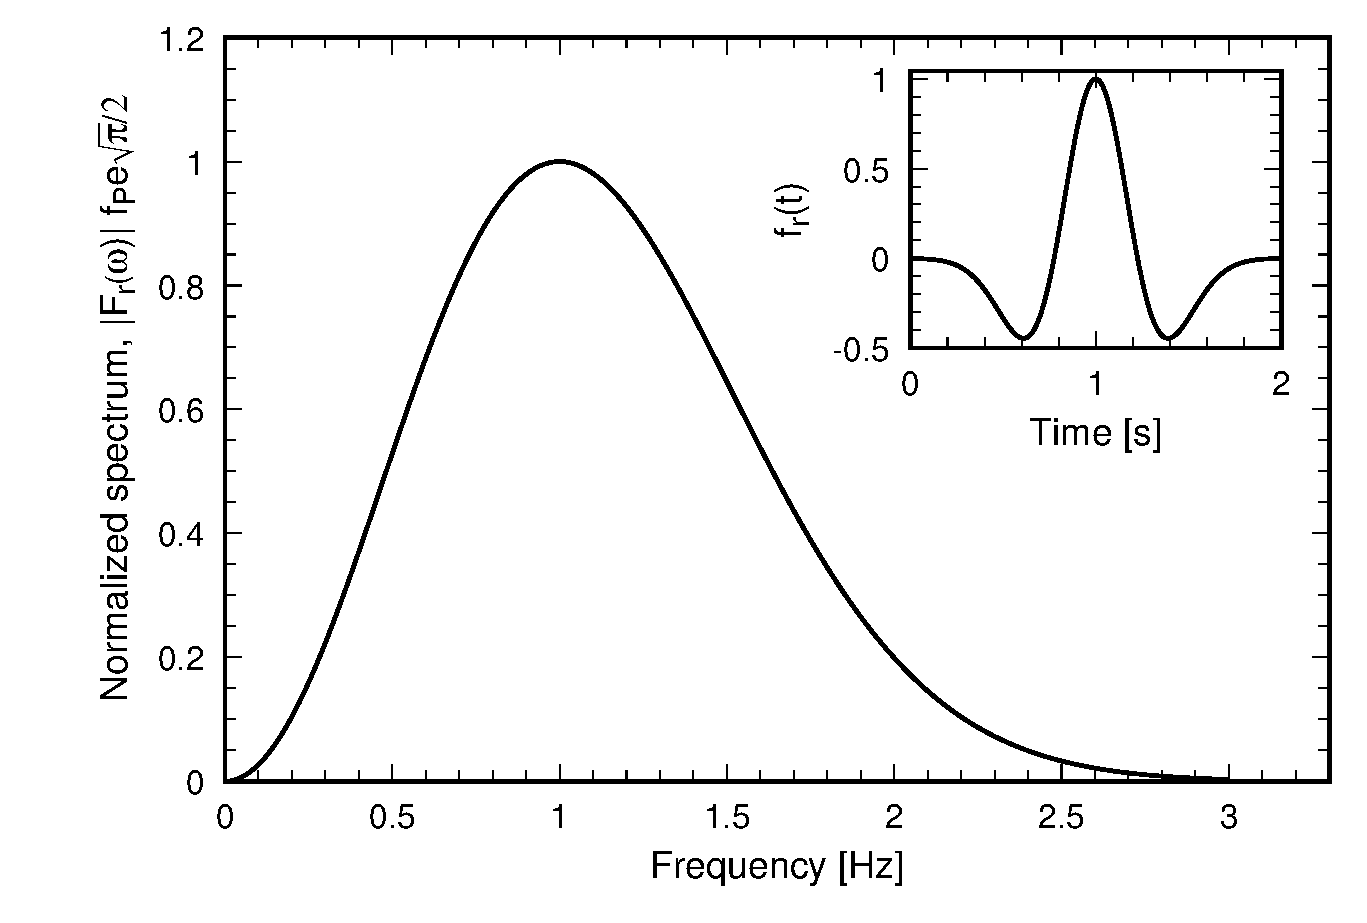
\epsfig{width=4.75in,%
            file=Figures/Fdtd-dimensionless/ricker-freq-time-print.eps}
  \end{center}
  \vspace{-.25in}
  \caption{Normalized spectrum of the Ricker wavelet with $f_P = 1$
  Hz.  The corresponding temporal form $f_r(t)$ is shown in the inset
  box where a delay of $1$ s has been assumed.  For other values of
  $f_P$, the horizontal axis in the time 
  domain is scaled by $1/f_P$.  For example, if $f_P$ were $1$ MHz,
  the peak would occur at $1$ $\mu$s rather than at $1$ s.  In the
  spectral domain, the horizontal axis is directly scaled by $f_P$ so
  that if $f_P$ were $1$ MHz, the peak would occur at $1$ MHz.}
  \label{fig:p-of-t-and-omega}
\end{figure}

The peak frequency $f_P$ has a corresponding wavelength $\lambda_P$.
This wavelength can be expressed in terms of the spatial step such
that $\lambda_P = N_P\Delx$, where $N_P$ does not need to be an
integer.  Thus
\begin{equation}
  f_P = \frac{c}{\lambda_P} = \frac{c}{N_P \Delx}
  \label{eq:peakExpression}
\end{equation}
The Courant number $S_c$ is $c\Delt/\Delx$ so the spatial step can be
expressed as $\Delx = c \Delt/S_c$.  Using this in
\refeq{eq:peakExpression} yields
\begin{equation}
  f_P = \frac{S_c}{N_P \Delt}.
  \label{eq:fp-equiv}
\end{equation}
The delay can thus be expressed as
\begin{equation}
  d_r = M_d\frac{1}{f_P} = M_d \frac{N_P \Delt}{S_c}.
 \label{eq:dr-equiv}
\end{equation}
Letting time $t$ be $q\Delt$ and expressing $f_P$ and $d_r$ as in
\refeq{eq:fp-equiv} and \refeq{eq:dr-equiv}, the discrete form of
\refeq{eq:rickerTime} can be written
as
\begin{equation}
  f_r[q] =
  \left(1-
  2 \pi^2 \left[\frac{S_c q}{N_P} - M_d\right]^2\right)
  \exp\left(-\pi^2 \left[\frac{S_c q}{N_P} - M_d\right]^2\right).
  \label{eq:rickerDiscrete}
\end{equation}
Note that the parameters that specify $f_r[q]$ are the Courant number
$S_c$, the points per wavelength at the peak frequency $N_P$, and the
delay multiple $M_d$---there is no $\Delt$ in
\refeq{eq:rickerDiscrete}.  This function appears to be independent of
the temporal and spatial steps, but it does depend on their ratio via
the Courant number $S_c$.

Equation \refeq{eq:rickerTime} gives the Ricker wavelet as a function
of only time.  However, as was discussed in Sec.\ \ref{sec:tfsf}, when
implementing a total-field/scattered-field boundary, it is necessary
to parameterize an incident field in both time and space.  As shown in
Sec.\ \ref{sec:waveEq}, one can always obtain a traveling plane-wave
solution to the wave equation simply by tweaking the argument of any
function that is twice differentiable.  Given the Ricker wavelet
$f_r(t)$, $f_r(t\pm x/c)$ is a solution to the wave equation where $c$
is the speed of propagation.  The plus sign corresponds to a wave
traveling in the negative $x$ direction and the negative sign
corresponds to a wave traveling in the positive $x$ direction.
(Although only 1D propagation will be considered here, this type
of tweaking can also be done in 2D and 3D.)  Therefore, a traveling
Ricker wavelet can be constructed by replacing the argument $t$ in
\refeq{eq:rickerTime} with $t\pm x/c$.  The value of the function now
depends on both time and location, i.e., it is a function of two
variables:
\begin{eqnarray}
f_r(t\pm x/c) & = & f_r(x,t), \nonumber \\
& = & \left(1-2 \pi^2 f_P^2 \left[t\pm\frac{x}{c}-d_r\right]^2\right)
       \exp\left(-\pi^2 f_P^2 \left[t\pm\frac{x}{c}-d_r\right]^2\right).
\end{eqnarray}
As before, \refeq{eq:dr-equiv} and \refeq{eq:fp-equiv} can be used to
rewrite $d_r$ and $f_P$ in terms of the Courant number, the points per
wavelength at the peak frequency, the temporal step, and the delay
multiple.  Replacing $t$ with $q\Delt$, $x$ with $m\Delx$, and
employing the identity $x/c = m\Delx/c = m\Delt/S_c$, yields
\begin{equation}
  f_r[m,q] =
  \left(1 - 2 \pi^2 \left[\frac{S_c q\pm m}{N_P} - M_d\right]^2\right)
  \exp\left(-\pi^2 \left[\frac{S_c q\pm m}{N_P} - M_d\right]^2\right).
  \label{eq:rickerDiscretex} 
\end{equation}
This gives the value of the Ricker wavelet at temporal index $q$ and
spatial index $m$.  Note that when $m$ is zero \refeq{eq:rickerDiscretex}
reduces to \refeq{eq:rickerDiscrete}.


\section{Mapping Frequencies to Discrete Fourier Transforms
\label{sec:fftMapping}}

Assume the field was recorded during an FDTD simulation and then the
recorded field was transformed to the frequency domain via a discrete
Fourier transform.  The discrete transform will yield a set of complex
numbers that represents the amplitude of discrete spectral components.
The question naturally arises: what is the correspondence between the
indices of the transformed set and the actual frequency?

In any simulation, the highest frequency $f_{\mathrm{max}}$ that can
exist is the inverse of the shortest period that can exist.  In a
discrete simulation one must have at least two samples per period.
Since the time samples are $\Delt$ apart, the shortest possible period
is $2\Delt$.  Therefore
\begin{equation}
  f_{\mathrm{max}} = \frac{1}{2\Delt}.
  \label{eq:fMax}
\end{equation}
The change in frequency from one discrete frequency to the next is the
spectral resolution $\Delf$.  The spectral resolution is dictated
by the total number of samples which we will call $N_T$ (an integer
value).  In general $N_T$ would correspond to the number of time steps
in an FDTD simulation.  The spectral resolution is given by
\begin{equation}
  \Delf = \frac{f_{\mathrm{max}}}{N_T/2}.
  \label{eq:delF}
\end{equation}
The factor of two is a consequence of the fact that there are both
positive and negative frequencies.  Thus one can think of the entire
spectrum as ranging from $-f_{\mathrm{max}}$ to $f_{\mathrm{max}}$,
i.e., an interval of $2f_{\mathrm{max}}$ which is then divided by
$N_T$.  Alternatively, to find $\Delf$ we can divide the maximum
positive frequency by $N_T/2$ as done in $\refeq{eq:delF}$.  Plugging
\refeq{eq:fMax} into \refeq{eq:delF} yields
\begin{equation}
  \Delf = \frac{1}{N_T\Delt}.
\end{equation}

In Sec.\ \ref{sec:harmonicSources} it was shown that a given frequency
$f$ could be written $c/\lambda=c/\ppw\Delx$ where $\ppw$ is the
number of points per wavelength (for the free-space wavelength).
After transforming to the spectral domain, this frequency would have a
corresponding index given by
\begin{equation}
  N_{\mathrm{freq}} = \frac{f}{\Delf} 
  = \frac{N_T c \Delt}{\ppw\Delx} 
  = \frac{N_T}{\ppw} \frac{c \Delt}{\Delx}
  = \frac{N_T}{\ppw} S_c.
  \label{eq:spectralIndex}
\end{equation}
Thus, the spectral index is dictated by the duration of the simulation
$N_T$, the Courant number $S_c$, and the points per wavelength $\ppw$.

Note that in practice different software packages may index things
differently.  The most typical practice is to have the first element
in the spectral array correspond to dc, the next $N_T/2$ elements
correspond to the positive frequencies, and then the next $(N_T/2)-1$
elements correspond to the negative frequencies (which will always be
the complex conjugates of the positive frequencies in any real FDTD
simulation).  The negative frequencies typically are stored from
highest frequency to lowest (i.e., fastest varying to slowest) so that
the last value in the array corresponds to the negative frequency
closest to dc ($-\Delf$).  Additionally, note that in 
\refeq{eq:spectralIndex} dc corresponds to an $N_{\mathrm{freq}}$ of
zero (since $\ppw$ is infinity for dc).  However when using Matlab the
dc term in the array obtained using the {\tt fft()} command has an
index of one.  The first element in the array has an index of
one---there is no ``zero'' element in Matlab arrays.  So, one must
understand and keep in mind the implementation details for a given
software package.

From \refeq{eq:fp-equiv}, the most energetic frequency in a Ricker
wavelet can be written
\begin{equation}
  f_P = \frac{S_c}{N_P \Delt}.
\end{equation}
The spectral index corresponding to this is given by
\begin{equation}
  N_{\mathrm{freq}} = \frac{f_P}{\Delf} 
  = \frac{N_T}{N_P}S_c.
\end{equation}
This is identical to \refeq{eq:spectralIndex} except the generic value
$\ppw$ has been replaced by $N_P$ which is the points per
wavelength at the peak frequency.

A discrete Fourier transform yields an array of numbers which
inherently has integer indices.  The array elements correspond to
discrete frequencies at multiples of $\Delf$.  However,
$N_{\mathrm{freq}}$ given in \refeq{eq:spectralIndex} need not be
thought of as an integer value.  As an example, assume there were
65536 times steps in a simulation in which the Courant number was
$1/\sqrt{2}$.  Further assume that we are interested in the frequency
which corresponds to $30$ points per wavelength ($\ppw=30$).  In this
case $N_{\mathrm{freq}}$ equals $65536/(30\sqrt{2}) = 1544.6983\cdots$.
There is no reason why one cannot think in terms of this particular
frequency.  However, this frequency is not directly available from a
discrete Fourier transform of the temporal data since the transform
will only have integer values of $N_{\mathrm{freq}}$.  For this
simulation an $N_{\mathrm{freq}}$ of $1544$ corresponds
$30.0136\cdots$ points per wavelength while an $N_{\mathrm{freq}}$ of
$1545$ corresponds $29.9941\cdots$ points per wavelength.  One can
interpolate between these values if the need is to measure the
spectral output right at $30$ points per wavelength.  

\section{Running Discrete Fourier Transform (DFT) \label{sec:dft}}

If one calculates the complete Fourier transform of the temporal data
of length $N_T$ points, one obtains information about the signal at
$N_T$ distinct frequencies (if one counts both positive and negative
frequencies).  However, much of that spectral information is of little
practical use.  Because of the dispersion error inherent in the FDTD
method and other numerical artifacts, one does not trust results
which correspond to frequencies with too coarse a discretization.
When taking the complete Fourier transform one often relies upon a
separate software package such as Mathematica, Matlab, or perhaps the
FFTw routines (a suite of very good C routines to perform discrete
Fourier transforms).  However, if one is only interested in obtaining
spectral information at a few frequencies, it is quite simple to
implement a discrete Fourier transform (DFT) which can be incorporated
directly into the FDTD code.  The DFT can be performed as the
simulation progresses and hence the temporal data does not have to be
recorded.  This section outlines the steps involved in computing such
a ``running DFT.''

Let us consider a discrete signal $g[q]$ which is, at least in theory,
periodic with a period of $N_T$ so that $g[q] = g[q+N_T]$ (in practice
only one period of the signal is of interest and this corresponds to
the data obtained from an FDTD simulation).  The discrete Fourier
series representation of this signal is
\begin{equation}
  g[q] = \sum_{k=\langle N_T\rangle} a_k e^{jk(2\pi/N_T)q}
  \label{eq:dftTime}
\end{equation}
where $k$ is an integer index and
\begin{equation}
  a_k = \frac{1}{N_T}
      \sum_{q=\langle N_T\rangle} g[q] e^{-jk(2\pi/N_T)q}
  \label{eq:dftAk}
\end{equation}
The summations are taken over $N_T$ consecutive points---we do not
care which ones, but in practice for our FDTD simulations $a_k$ would
be calculated with $q$ ranging from $0$ to $N_T-1$ (the term below the
summation symbols in \refeq{eq:dftTime} and \refeq{eq:dftAk}
indicates the summations are done over $N_T$ consecutive integers, but
the actual start and stop points do not matter).  The term $a_k$ gives
the spectral content at the frequency $f = k\Delf = k/(N_T\Delt)$.
Note that $a_k$ is obtained simply by taking the sum of the sequence
$g[q]$ weighted by an exponential.

The exponential in \refeq{eq:dftAk} can be written in terms of real
and imaginary parts, i.e., 
\begin{eqnarray}
  \Re[a_k] &=& \frac{1}{N_T} 
           \sum_{q=0}^{N_T - 1} g[q] \cos\!\left(\frac{2\pi k}{N_T}q\right), \\
  \Im[a_k] &=& -\frac{1}{N_T - 1}
           \sum_{q=0}^{N_T} g[q] \sin\!\left(\frac{2\pi k}{N_T}q\right),
\end{eqnarray}
where $\Re[]$ indicates the real part and $\Im[]$ indicates the
imaginary part.  In practice, $g[q]$ would be a particular field
component and these calculations would be performed concurrently with
the time-stepping.  The value of $\Re[a_k]$ would be initialized to
zero.  Then, at each time step $\Re[a_k]$ would be set equal to its
previous value plus the current value of $g[q] \cos(2\pi k q/N_T)$,
i.e., we would perform a running sum.  Once the time-stepping
has completed, the stored value of $\Re[a_k]$ would be divided by $N_T$.
A similar procedure is followed for $\Im[a_k]$ where the only
difference is that the value used in the running sum is $-g[q]
\sin(2\pi k q/N_T)$.  Note that the factor $2\pi k/N_T$ is a constant
for a particular frequency, i.e., for a particular $k$.

Similar to the example at the end of the previous section, let us
consider how we would extract information at a few specific
discretizations.  Assume that $N_T = 8192$ and $S_c=1/\sqrt{2}$.
Further assume we want to find the spectral content of a particular
field for discretizations of $N_\lambda = 20$, $30$, $40$, and $50$
points per wavelength.  Plugging these values into
\refeq{eq:spectralIndex} yields corresponding spectral indices
(i.e., $N_{\mathrm{freq}}$ or index $k$ in \refeq{eq:dftAk}) of
\begin{eqnarray*}
N_\lambda = 20 &\Rightarrow& k = 289.631, \\
N_\lambda = 30 &\Rightarrow& k = 193.087, \\
N_\lambda = 40 &\Rightarrow& k = 144.815, \\
N_\lambda = 50 &\Rightarrow& k = 115.852. 
\end{eqnarray*}
The spectral index must be an integer.  Therefore, rounding $k$ to the
nearest integer and solving for the corresponding $N_\lambda$ we find
\begin{eqnarray*}
k = 290 & \Rightarrow & N_\lambda = 19.9745, \\ 
k = 193 & \Rightarrow & N_\lambda = 30.0136, \\ 
k = 145 & \Rightarrow & N_\lambda = 39.9491, \\ 
k = 116 & \Rightarrow & N_\lambda = 49.9364. 
\end{eqnarray*}
Note that these values of $N_\lambda$ differ slightly from the
``desired'' values.  Assume that we are modeling an object with some
characteristic dimension of twenty cells, i.e., $a = 20\Delx$.  Given
the initial list of integer $N_\lambda$ values, we could say that we
were interested in finding the field at frequencies with corresponding
wavelengths of $a$, $\frac{3}{2}a$, $2a$, and $\frac{5}{2}a$.
However, using the non-integer $N_\lambda$'s that are listed above,
the values we obtain correspond to $0.99877 a$, $1.500678a$, $1.997455
a$, and $2.496818 a$.  As long as one is aware of what is actually
being calculated, this should not be a problem.  Of course, as
mentioned previously, if we want to get closer to the desired values,
we can interpolate between the two spectral indices which bracket the
desired value.

\section{Real Signals and DFT's}

In nearly all FDTD simulations we are concerned with real signals,
i.e., $g[q]$ in \refeq{eq:dftTime} and \refeq{eq:dftAk} are real.  For
a given spectral index $k$ (which can be thought of as a frequency),
the spectral coefficient $a_k$ is as given in \refeq{eq:dftAk}.  Now,
consider an index of $N_T - k$.  In this case the value of $a_{N_T -
  k}$ is given by
\begin{align}
  a_{N_T - k} = &= \frac{1}{N_T}
    \sum_{q=\langle N_T\rangle} g[q] e^{-j(N_T-k)(2\pi/N_T)q}, \nonumber \\
  &= \frac{1}{N_T}
    \sum_{q=\langle N_T\rangle} g[q] e^{-j2\pi}e^{jk(2\pi/N_T)q}, \nonumber \\
  &= \frac{1}{N_T}
    \sum_{q=\langle N_T\rangle} g[q] e^{jk(2\pi/N_T)q}, \nonumber \\
a_{N_T - k} &= a_k^*,
\end{align}
where $a_k^*$ is the complex conjugate of $a_k$.  Thus, for real
signals, the calculation of one value of $a_k$ actually provides the
value of two coefficients: the one for index $k$ and the one for index
$N_T-k$.

Another important thing to note is that, similar to the continuous
Fourier transform where there are positive and negative frequencies,
with the discrete Fourier transform there are also pairs of
frequencies that should typically be considered together.  Let us
assume that index $k$ goes from $0$ to $N_T-1$.  The $k=0$ frequency
is dc.  Assuming $N_T$ is even, $k=N_T/2$ is the Nyquist frequency where
the spectral basis function $\exp(j\pi q)$ alternates between positive
and negative one at each successive time-step.  Both $a_0$ and
$a_{N_T/2}$ will be real.  All other spectral components can be
complex, but for real signals it will always be true that $a_{N_T-k} =
a_k^*$.

If we are interested in the amplitude of a spectral component at a
frequency of $k$, we really need to consider the contribution from
both $k$ and $N_T-k$ since the oscillation at both these indices is at
the same frequency.  Let us assume we are interested in reconstructing
just the $k'$th frequency of a signal.  The spectral components would
be given in the time domain by
\begin{align}
  f[q] &= a_{k'} e^{jk'(2\pi/N_T)q} + a_{N_T-k'} e^{j(N_T-k')(2\pi/N_T)q} \nonumber\\
       &= a_{k'} e^{jk'(2\pi/N_T)q} + a_{k'}^* e^{j2\pi} e^{-jk'(2\pi/N_T)q} \nonumber\\
       &= 2 \Re[a_{k'}]\cos\!\left(\frac{2k'\pi}{N_T}q\right) 
        - 2 \Im[a_{k'}]\sin\!\left(\frac{2k'\pi}{N_T}q\right) \nonumber\\
       &= 2 |a_{k'}| \cos\!\left(\frac{2k'\pi}{N_T}q + 
          \tan^{-1}\!\left(\frac{\Im[a_{k'}]}{\Re[a_{k'}]}\right)\right) 
\end{align}
Thus, importantly, the amplitude of this harmonic function is given by
$2|a_{k'}|$ (and not merely $|a_{k'}|$).

Let us explore this further by considering the $x$ component of an
electric field at some arbitrary point that is given by
\begin{align}
  \Evec[q] &= E_{x0} \cos[\omega_{k'} q + \theta_e] \unitvec{x}, \nonumber \\
     &= \Re[E_{x0} e^{j\theta_e} e^{j\omega_{k'} q}] \unitvec{x}, \nonumber \\
     &= \frac{1}{2}[\hE_{x0} e^{j\omega_{k'} q} +
                    \hE_{x0}^* e^{-j\omega_{k'} q}] \unitvec{x},
   \label{eq:eForDft}
\end{align}
where 
\begin{align}
  \omega_{k'}  &= k' \frac{2\pi}{N_T}, \\
  \hE_{x0} &= E_{x0} e^{j\theta_e},
\end{align}
and $k'$ is some arbitrary integer constant.  Plugging
\refeq{eq:eForDft} into \refeq{eq:dftAk} and dropping the unit vector
yields
\begin{align}
  a_k &= \frac{1}{2N_T}
     \sum_{q=\langle N_T\rangle} 
     [\hE_{x0} e^{j\omega_{k'} q} + \hE_{x0}^* e^{-j\omega_{k'} q}]
     e^{-j\omega_k q}, \nonumber \\
  &=
    \frac{1}{2N_T}
     \sum_{q=\langle N_T\rangle} 
     [\hE_{x0} e^{j(\omega_{k'}-\omega_{k}) q} 
     + \hE_{x0}^* e^{-j(\omega_{k'} + \omega_{k}) q}], \nonumber \\
  &=
    \frac{1}{2N_T}
     \sum_{q=\langle N_T\rangle} 
     [\hE_{x0} e^{j(k' - k)(2\pi/N_T) q} 
       + \hE_{x0}^* e^{-j(k' + k)(2\pi/N_T) q}].
   \label{eq:akForSingleFreq}
\end{align}

Without loss of generality, let us now assume $q$ varies between $0$
and $N_T-1$ while $k$ and $k'$ are restricted to be between $0$ and
$N_T-1$.  Noting the following relationship for geometric series
\begin{equation}
\sum_{q=0}^{N-1} x^q = 1 + x + x^2 + \cdots + x^{N-1} =  \frac{1-x^N}{1-x}
\end{equation}
we can express the sum of the first exponential expression in
\refeq{eq:akForSingleFreq} as
\begin{equation}
  \sum_{q=0}^{N_T-1} e^{j(k' - k)(2\pi/N_T) q}
  =
  \frac{1 - e^{j(k' - k)2\pi}}
       {1 - e^{j(k' - k)(2\pi/N_T)}}.
  \label{eq:sumExponentsI}
\end{equation}
Since $k$ and $k'$ are integers, the second term in the numerator on
the right side, $\exp(j(k' - k)2\pi)$, equals $1$ for all values of
$k$ and $k'$ and thus this numerator is always zero.  Provided $k\neq
k'$, the denominator is non-zero and we conclude that for $k\neq k'$
the sum is zero.  For $k = k'$, the denominator is also zero and hence
the expression on the right does not provide a convenient way to
determine the value of the sum.  However, when $k=k'$ the terms being
summed are simply $1$ for all values of $q$.  Since there are $N_T$
terms, the sum is $N_T$.  Given this, we can write the ``orthogonality
relationship'' for the exponentials
\begin{equation}
  \sum_{q=0}^{N_T-1} e^{j(k' - k)(2\pi/N_T) q} 
  =
\left\{
  \begin{array}{cl}
     0    &  \quad k'\neq k \\
     N_T  &  \quad k' = k
  \end{array}
\right.
\end{equation}
Using this orthogonality relationship in
\refeq{eq:akForSingleFreq}, we find that for the harmonic signal given
in \refeq{eq:eForDft}, one of the non-zero spectral coefficients is
\begin{equation}
  a_{k'} = \frac{1}{2} \hE_{x0}.
\end{equation}
Conversely, expressing the (complex) amplitude in terms of the
spectral coefficient from the DFT, we have
\begin{equation}
  \hE_{x0} = 2 a_{k'}.
\end{equation}

For the sake of completeness, now consider the sum of the other
complex exponential term in \refeq{eq:akForSingleFreq}.  Here the
orthogonality relationship is
\begin{equation}
  \sum_{q=0}^{N_T-1} e^{-j(k' + k)(2\pi/N_T) q} 
  =
\left\{
  \begin{array}{cl}
     0    &  \quad k\neq N_T - k' \\
     N_T  &  \quad k = N_T - k' 
  \end{array}
\right.
\end{equation}
Using this in \refeq{eq:akForSingleFreq} tells us
\begin{equation}
  a_{N_T - k'} = \frac{1}{2} \hE_{x0}^*.
\end{equation}
Or, expressing the (complex) amplitude in terms of this spectral
coefficient from the DFT, we have
\begin{equation}
  \hE_{x0} = 2 a_{N_T - k'}^*.
\end{equation}

Now, let us consider the calculation of the time-averaged Poynting
vector $\Pvec_{\mathrm avg}$ which is given by
\begin{equation}
  \Pvec_{\mathrm avg} = 
  \frac{1}{2}\Re\!\left[\hat{\Evec} \times \hat{\Hvec}^* \right]
\end{equation}
where the carat indicates the phasor representation of the field,
i.e.,
\begin{align}
\hat{\Evec} &=
  \hE_{x0} \unitvec{x} +
  \hE_{y0} \unitvec{y} +
  \hE_{z0} \unitvec{z}, \nonumber \\
  &= 2 a_{e,x,k} \unitvec{x} +
     2 a_{e,y,k} \unitvec{y} +
     2 a_{e,z,k} \unitvec{z}
\end{align}
where $a_{e,w,k}$ is the $k$th spectral coefficient for the $w$
component of the electric field with $w\in \left\{x,y,z\right\}$.
Defining things similarly for the magnetic field yields
\begin{align}
\hat{\Hvec} &=
  \hH_{x0} \unitvec{x} +
  \hH_{y0} \unitvec{y} +
  \hH_{z0} \unitvec{z}, \nonumber \\
  &= 2 a_{h,x,k} \unitvec{x} +
     2 a_{h,y,k} \unitvec{y} +
     2 a_{h,z,k} \unitvec{z}.
\end{align}
The time-averaged Poynting vector can now be written in terms of the
spectral coefficients as
\begin{align}
  \Pvec_{\mathrm avg} = 
  2 \, \Re\biggl[
  &\left[a_{e,y,k}a_{h,z,k}^* - a_{e,z,k}a_{h,y,k}^*\right] \unitvec{x} +
  \left[a_{e,z,k}a_{h,x,k}^* - a_{e,x,k}a_{h,z,k}^*\right] \unitvec{y}
  + \mbox{}
  \nonumber \\
  &\left[a_{e,x,k}a_{h,y,k}^* - a_{e,y,k}a_{h,x,k}^*\right] \unitvec{z}
  \biggr].
\end{align}
Thus, importantly, when directly using these DFT coefficients in the
calculation of the Poynting vector, instead of the usual ``one-half
the real part of E cross H,'' the correct expression is ``two times
the real part of E cross H.''

\section{Amplitude and Phase from Two Time-Domain
  Samples \label{sec:twosamples}}

In some applications the FDTD method is used in a quasi-harmonic way,
meaning the source is turned on, or ramped up, and then run
continuously in a harmonic way until the simulation is terminated.
Although this prevents one from obtaining broad spectrum output, for
applications that have highly inhomogeneous media and where only a
single frequency is of interest, the FDTD method used in a
quasi-harmonic way may still be the best numerical tool to analyze the
problem.  The FDTD method is often used in this when in the study of
the interaction of electromagnetic fields with the human body.
(Tissues in the human body are typically quite dispersive.
Implementing dispersive models that accurately describe this
dispersion over a broad spectrum can be quite challenging.  When using
a quasi-harmonic approach one can simply use constant coefficients for
the material constants, i.e., use the values that pertain at the
frequency of interest which also corresponds to the frequency of the
excitation.)

When doing a quasi-harmonic simulation, the simulation terminates when
the fields have reached steady state.  Steady state can be defined as
the time beyond which temporal changes in the amplitude and phase of
the fields are negligibly small.  Thus, one needs to know the amplitude
and phase of the fields at various points.  Fortunately the amplitude
and phase can be calculated from only two sample points of the
time-domain field.

Let us assume the field at some point $(x,y,z)$ is varying harmonically as
\begin{equation}
  f(x,y,z,t) = A(x,y,z) \cos(\omega t + \phi(x,y,z)).
\end{equation}
where $A$ is the amplitude and $\phi$ is the phase, both of which are
initially unknown.  We will drop the explicit argument of space in the
following with the understanding that we are talking about the field
at a fixed point.

Consider two different samples of the field in time
\begin{eqnarray}
  f(t_1) &=& f_1 \, = \, A \cos(\omega t_1 + \phi), \\
  f(t_2) &=& f_2 \, = \, A \cos(\omega t_2 + \phi).
\end{eqnarray}
We will assume that the samples are taken roughly a quarter of a cycle
apart to ensure the samples are never simultaneously zero.  A quarter
of a cycle is given by $T/4$ where $T$ is the period.  We can express
this in terms of time steps as
\begin{equation}
\frac{T}{4} =
 \frac{1}{4f} = 
 \frac{\lambda}{4c} = 
 \frac{N_\lambda \Delx}{4c}\frac{\Delt}{\Delt} = 
 \frac{N_\lambda}{4S_c} \Delt.
\end{equation}
Since we only allow an integer number of time-steps between $t_1$ and
$t_2$, the temporal separation between $t_1$ and $t_2$ would be
$\mbox{int}(N_\lambda/4S_c)$ time-steps.

Given these two samples, $f_1$ and $f_2$, we wish to determine $A$ and
$\phi$.  Using the trig identity for the cosine of the sum of two
values, we can express these fields as
\begin{eqnarray}
  f_1 & = & A (\cos(\omega t_1)\cos(\phi) - \sin(\omega t_1)\sin(\phi)),
  \label{eq:fieldSampleOne} \\
  f_2 & = & A (\cos(\omega t_2)\cos(\phi) - \sin(\omega t_2)\sin(\phi)).
  \label{eq:fieldSampleTwo}
\end{eqnarray}
We are assuming that $f_1$ and $f_2$ are known and we know the times
at which the samples were taken.  Using \refeq{eq:fieldSampleOne} to
solve for $A$ we obtain
\begin{equation}
  A = \frac{f_1}{\cos(\omega t_1)\cos(\phi) - \sin(\omega t_1)\sin(\phi)}.
  \label{eq:ampEqOne}
\end{equation}
Plugging \refeq{eq:ampEqOne} into \refeq{eq:fieldSampleTwo} and
rearranging terms ultimately leads to
\begin{equation}
\frac{\sin(\phi)}{\cos(\phi)} = 
\tan(\phi) = \frac{f_2\cos(\omega t_1) - f_1\cos(\omega t_2)}
                  {f_2\sin(\omega t_1) - f_1\sin(\omega t_2)}.
  \label{eq:phaseEqOne}
\end{equation}
The time at which we take the first sample, $t_1$, is almost always
arbitrary.  We are free to call that ``time zero,'' i.e., $t_1=0$.  By
doing this we have $\cos(\omega t_1) = 1$ and $\sin(\omega t_1) = 0$.  
Using these values in \refeq{eq:phaseEqOne} and \refeq{eq:ampEqOne}
yields
\begin{equation}
  \phi = \tan^{-1}\!
  \left(\frac{\cos(\omega t_2) - \frac{f_2}{f_1}}{\sin(\omega t_2)}\right),
  \label{eq:phaseEqTwo}
\end{equation}
and
\begin{equation}
   A = \frac{f_1}{\cos(\phi)}.
  \label{eq:ampEqTwo}
\end{equation}
Note that these equations assume that $f_1\neq 0$ and, similarly, that
$\phi\neq \pm\pi/2$ radians (which is the same as requiring that
$\cos(\phi)\neq 0$).

If $f_1$ is identically zero, we can say that $\phi$ is $\pm\pi/2$
(where the sign can be determined by the other sample point:
$\phi=-\pi/2$ if $f_2>0$ and $\phi=+\pi/2$ if $f_2<0$).  If $f_1$ is
not identically zero, we can use \refeq{eq:phaseEqTwo} to calculate
the phase since the inverse tangent function has no problem with large
arguments.  However, if the phase is close to $\pm\pi/2$, the
amplitude as calculated by \refeq{eq:ampEqTwo} would involve the
division of two small numbers which is generally not a good way to
determine a value.  Rather than doing this, we can use
\refeq{eq:fieldSampleTwo} to express the amplitude as
\begin{equation}
  A = \frac{f_2}{\cos(\omega t_2)\cos(\phi) - \sin(\omega t_2)\sin(\phi)}.
  \label{eq:ampEqThree}
\end{equation}
This equation should perform well when the phase is close to $\pm\pi/2$.

At this point we have the following expressions for the phase and
magnitude (the reason for adding a prime to the phase and magnitude
will become evident shortly):
\begin{equation}
  \phi' = \left\{
  \begin{array}{ll}
  -\pi/2 & \mbox{if $f_1 = 0$ and $f_2 > 0$} \\
  \pi/2 & \mbox{if $f_1 = 0$ and $f_2 < 0$} \\
  \tan^{-1}\!
  \left(\frac{\cos(\omega t_2) - \frac{f_2}{f_1}}
       {\sin(\omega t_2)}\right)
  & \mbox{otherwise}
  \end{array}
  \right.
\end{equation}
and
\begin{equation}
  A' = \left\{
  \begin{array}{ll}
   \frac{f_1}{\cos(\phi')} & \mbox{if $|f_1| \geq |f_2|$} \\
   \frac{f_2}{\cos(\omega t_2)\cos(\phi') - \sin(\omega t_2)\sin(\phi')}
   & \mbox{otherwise}
  \end{array}
  \right.
  \label{eq:ampEqFour}
\end{equation}
There is one final step in calculating the magnitude and phase.  The
inverse-tangent function returns values between $-\pi/2$ and $\pi/2$.
As given by \refeq{eq:ampEqFour}, the amplitude $A'$ can be either
positive or negative.  Generally we think of phase as varying between
$-\pi$ and $\pi$ and assume the amplitude is non-negative.
To obtained such values we can obtain the final values for the
amplitude and phase as follows
\begin{equation}
  (A,\phi) = \left\{
  \begin{array}{ll}
   (A',\phi') & \mbox{if $A'>0$} \\
   (-A',\phi'-\pi) & \mbox{if $A'<0$ and $\phi'\geq 0$} \\
   (-A',\phi'+\pi) & \mbox{if $A'<0$ and $\phi'< 0$} \\
  \end{array}
  \right.
  \label{eq:ampPhaseFinal}
\end{equation}

Finally, we have assumed that $t_1=0$.  Correspondingly, that means
that $t_2$ can be expressed as $t_2=N_2\Delt$ where $N_2$ is the
(integer) number of time steps between the samples $f_1$ and $f_2$.
Thus the argument of the trig functions above can be written as
\begin{equation}
  \omega t_2 = 2\pi S_c \frac{N_2}{N_\lambda}
\end{equation}
where $N_\lambda$ is the number of points per wavelength of the
excitation (and frequency of interest).

\section{Conductivity \label{sec:conductivity}}

When a material is lossless, the phase constant $\beta$ for a harmonic
plane wave is given by $\omega\sqrt{\mu\epsilon}$ and the spatial
dependence is given by $\exp(\pm j\beta x)$.  When the material has a
non-zero electrical conductivity ($\sigma\neq 0$), the material is
lossy and the wave experiences exponential decay as it propagates.
The spatial dependence is given by $\exp(\pm\gamma x)$ where
\begin{equation}
  \gamma = j\omega\sqrt{\mu\epsilon
                       \left(1-j\frac{\sigma}{\omega\epsilon}\right)}
         = \alpha+j\beta
\end{equation}
where $\alpha$ (the real part of $\gamma$) is the attenuation constant
and $\beta$ (the imaginary part of $\gamma$) is the phase constant.
The attenuation and phase constants can be expressed directly in terms
of the material parameters and the frequency:
\begin{eqnarray}
  \alpha &=& \frac{\omega\sqrt{\mu\epsilon}}{\sqrt{2}}
   \left(\left[1+\left(\frac{\sigma}{\omega\epsilon}\right)^2\right]^{1/2}
   -1\right)^{1/2},
  \label{eq:alpha}
 \\
  \beta &=& \frac{\omega\sqrt{\mu\epsilon}}{\sqrt{2}}
   \left(\left[1+\left(\frac{\sigma}{\omega\epsilon}\right)^2\right]^{1/2}
   +1\right)^{1/2}.
  \label{eq:lossyK}
\end{eqnarray}
When the conductivity is zero, the attenuation constant is zero and
the phase constant reduces to that of the lossless case, i.e.,
$\gamma=j\beta=j\omega\sqrt{\mu\epsilon}$.

Assume a wave is propagating in the positive $x$ direction in a
material with non-zero electrical conductivity.  The wave amplitude
will decay as $\exp(-\alpha x)$.  The skin depth $\skin$ is the
distance over which the wave decays an amount $1/e$.  Starting with a
reference point of $x=0$, the fields would have decayed an amount
$1/e$ when $x$ is $1/\alpha$ (so that the exponent is simply $-1$).
Thus, $\skin$ is given by
\begin{equation}
  \skin = \frac{1}{\alpha}.
\end{equation}
Since the skin depth is merely a distance, it can be expressed in
terms of the spatial step, i.e., 
\begin{equation}
  \skin = \frac{1}{\alpha}= N_L\Delx
\end{equation}
where $N_L$ is the number of spatial steps in the skin depth (think of
the subscript $L$ as standing for loss).  $N_L$ does not need to be an
integer.

It is possible to use \refeq{eq:alpha} to solve for the conductivity
in terms of the attenuation constant.  The resulting expression is
\begin{equation}
  \sigma = \omega\epsilon
    \left(\left[1+\frac{2\alpha^2}{\omega^2\mu\epsilon}\right]^2
          - 1\right)^{1/2}.
  \label{eq:sigmaAlpha}
\end{equation}
As shown in Sec.\ \ref{sec:loss}, when the electrical conductivity is
non-zero the electric-field update equation contains the term
$\sigma\Delt/2\epsilon$.  Multiplying both side of
\refeq{eq:sigmaAlpha} by $\Delt/2\epsilon$ yields
\begin{equation}
  \frac{\sigma\Delt}{2\epsilon} = \frac{\omega\Delt}{2}
    \left(\left[1+\frac{2\alpha^2}{\omega^2\mu\epsilon}\right]^2
          - 1\right)^{1/2}.
  \label{eq:lossCoef}
\end{equation}
Assume that one wants to obtain a certain skin depth (or decay rate)
at a particular frequency which is discretized with $\ppw$ points per
wavelength, i.e., $\omega=2\pi f=2\pi c/\ppw \Delx$.  Thus the term
$\omega\Delt/2$ can be rewritten
\begin{equation}
  \frac{\omega\Delt}{2} = \frac{\pi}{\ppw}\frac{c\Delt}{\Delx}
                        = \frac{\pi}{\ppw}S_c.
  \label{eq:lossTerm}
\end{equation}
Similarly, using the same expression for $\omega$ and using
$\alpha=1/N_L\Delx$, one can write
\begin{equation}
  \frac{2\alpha^2}{\omega^2\mu\epsilon} =
   \frac{2 \left(\frac{1}{N_L\Delx}\right)^2}
        {\left(\frac{2\pi c}{\ppw \Delx}\right)^2
         \mu_0\mu_r\epsilon_0\epsilon_r} = 
   \frac{\ppw^2}{2 \pi^2 N_L^2 \epsilon_r\mu_r}.
  \label{eq:lossTermI}
\end{equation}
Using \refeq{eq:lossTerm} and \refeq{eq:lossTermI} in 
\refeq{eq:lossCoef} yields
\begin{equation}
  \frac{\sigma\Delt}{2\epsilon} = 
    \frac{\pi}{\ppw}S_c
    \left(\left[1+\frac{\ppw^2}{2 \pi^2 N_L^2 \epsilon_r\mu_r}\right]^2
          - 1\right)^{1/2}.
  \label{eq:lossCoefI}
\end{equation}
Note that neither the temporal nor the spatial steps appear in the
right-hand side.

As an example how \refeq{eq:lossCoefI} can be used, assume that one
wants a skin depth of $20 \Delx$ for a wavelength of $40\Delx$. Thus
$N_L=20$ and $\ppw=40$ and the skin depth is one half of the
free-space wavelength.  Further assume the Courant number $S_c$ is
unity, $\epsilon_r=4$, and $\mu_r=1$.  Plugging these values into
\refeq{eq:lossCoefI} yields $\sigma\Delt/2\epsilon=0.0253146$.

Let us write a program where a TFSF boundary introduces a sine wave
with a frequency that is discretized at $40$ points per wavelength.
We will only implement electrical loss (the magnetic conductivity is
zero).  Snapshots will be taken every time step after the temporal
index is within $40$ steps from the final time step.  The lossy layer
starts at node $100$.  To implement this program, we can re-use nearly
all the code that was described in Sec.\ \ref{sec:improveThree}.  To
implement this, we merely have to change the {\tt gridInit3()}
function and the functions associated with the source function.  The
new {\tt gridInit3()} function is shown in Program
\ref{pro:gridinitlossy}.  The harmonic source function is given by the
code presented in Program \ref{pro:ezincharm}.

\begin{program}
{\tt gridinitlossy.c} A {\tt Grid} initialization function for
modeling a lossy half space.  Here the conductivity results in a skin
depth of $20$ cells for an excitation that is discretized using $40$
cells per wavelength. \label{pro:gridinitlossy}
\codemiddle
\begin{lstlisting}
#include "fdtd3.h"

#define LOSS 0.0253146
#define LOSS_LAYER 100
#define EPSR 4.0 

void gridInit3(Grid *g) {
  double imp0 = 377.0;
  int mm;

  SizeX = 200;   // size of domain
  MaxTime = 450; // duration of simulation
  Cdtds = 1.0;   // Courant number

  /* Allocate memory for arrays. */
  ALLOC_1D(g->ez,   SizeX, double);
  ALLOC_1D(g->ceze, SizeX, double);
  ALLOC_1D(g->cezh, SizeX, double);
  ALLOC_1D(g->hy,   SizeX - 1, double);
  ALLOC_1D(g->chyh, SizeX - 1, double);
  ALLOC_1D(g->chye, SizeX - 1, double);

  /* set electric-field update coefficients */
  for (mm=0; mm < SizeX; mm++)
    if (mm < 100) {
      Ceze(mm) = 1.0;
      Cezh(mm) = imp0;
    } else {
      Ceze(mm) = (1.0 - LOSS) / (1.0 + LOSS);
      Cezh(mm) = imp0 / EPSR / (1.0 + LOSS);
    }

  /* set magnetic-field update coefficients */
  for (mm=0; mm < SizeX - 1; mm++) {
    Chyh(mm) = 1.0;
    Chye(mm) = 1.0 / imp0;
  }

  return;
}
\end{lstlisting}
\end{program}

\begin{program} {\tt ezincharm.c} Functions to implement a harmonic
  source.  When initialized, the user is prompted to enter the number
  of points per wavelength (in the results to follow it is assumed the
  user enters $40$). \label{pro:ezincharm} \codemiddle
\begin{lstlisting}
#include "ezinc3.h"

/* global variables -- but private to this file */
static double ppw = 0, cdtds;

/* prompt user for source-function points per wavelength */
void ezIncInit(Grid *g){

  cdtds = Cdtds;  
  printf("Enter points per wavelength: ");
  scanf(" %lf", &ppw);

  return;
}

/* calculate source function at given time and location */
double ezInc(double time, double location) {
  if (ppw <= 0) {
    fprintf(stderr,
       "ezInc: must call ezIncInit before ezInc.\n"
       "       Points per wavelength must be positive.\n");
    exit(-1);
  }

  return sin(2.0 * M_PI / ppw * (cdtds * time - location));
}
\end{lstlisting}
\end{program}


Assuming the user specified that the TFSF boundary should be at node
$50$ and there should be $40$ points per wavelength for the harmonic
source, Fig. \ref{fig:decayDemo}(a) shows the resulting maximum of the
magnitude of the electric field as a function of position.  For each
position, all the snapshots were inspected and the maximum recorded.
Figure \ref{fig:decayDemo}(b) shows a superposition of $41$ snapshots
taken one time-step apart.  One can see the exponential decay starting
at node $100$.  Between node $50$ and node $100$ there is a
standing-wave pattern caused by the interference of the incident and
reflected waves.  From the start of the grid to node $50$ the
magnitude is flat.  This is caused by the fact that there is only
scattered field here---there is nothing to interfere with the
reflected wave and we see the constant amplitude associated with a
pure traveling wave.  The ratio of the amplitude at nodes $120$ and
$100$ was found to be $0.3644$ whereas the ideal value of $1/e$ is
$0.3679$ (thus there is approximately a one percent error in this
simulation).

\begin{figure}
  \begin{center}
  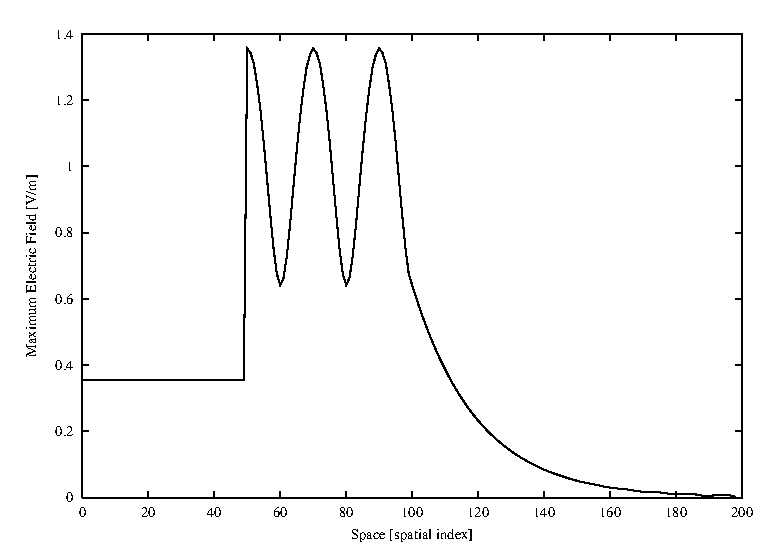
\epsfig{width=4.2in,file=Code/Fdtd-dimensionless/envelope.eps} \\
  (a) \\ \vspace{.2in}
  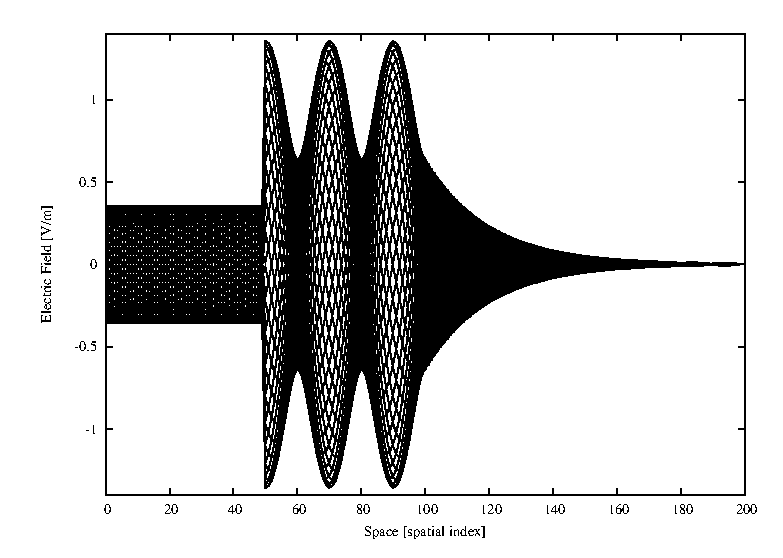
\epsfig{width=4.2in,file=Code/Fdtd-dimensionless/all-snapshots.eps}
  \\ (b) \end{center} \caption{(a) Maximum electric field magnitude
  that exists at each point (obtained by obtaining the maximum value
  in all the snapshots).  The flat line over the first $50$ nodes
  corresponds to the scattered-field region.  The reflected field
  travels without decay and hence produces the flat line.  The
  total-field region between nodes $50$ and $100$ contains a
  standing-wave pattern caused by the interference of the incident and
  scattered fields.  There is exponential decay of the fields beyond
  node $100$ which is where the lossy layer starts.  (b) Superposition
  of $41$ individual snapshots of the field which illustrates the
  envelope of the field.}  \label{fig:decayDemo}
\end{figure}

% Figure generate with using matlab with following commands:
% z=readOneD('sim');
% for i=1:200              
%   zmax(i)=max(abs(z(:,i)));
% end                      
% plot(zmax)
% xlabel('Space [spatial index]')
% ylabel('Maximum of Electric Field Magnitude')

If one were interested in non-zero magnetic conductivity $\sigma_m$,
the loss term which appears in the magnetic-field update equations is
$\sigma_m\Delt/2\mu$.  This term can be handled in exactly the same
way as the term resulting from electric conductivity.  


\section[Transmission Coefficient for a Planar Interface]%
{Example:  Obtaining the Transmission Coefficient for a Planar
Interface \label{sec:specExampleTrans}}

In this last section, we demonstrate how the transmission coefficient
for a planar dielectric boundary can be obtained from the FDTD method.
This serves to highlight many of the points that were considered in
the previous section.  We will compare the results to the exact
solution.  The disparity between the two provides motivation to
determine the dispersion relation in the FDTD (which is covered in
Chap.\ \ref{chap:dispersion}).

The majority of instructional material concerning electromagnetics is
expressed in terms of harmonic, or frequency-domain, signals.  A
temporal dependence of $\exp(j\omega t)$ is understood and therefore
one only has to consider the spatial variation.  In the frequency
domain, the fields and quantities such as the propagation constant and
the characteristic impedance are represented by complex numbers.
These complex numbers give the magnitude and phase of the value and
will be functions of frequency.  In the following discussion a caret
(hat) will be used to indicate a complex quantity and one should keep
in mind that complex numbers are inherently tied to the frequency
domain.  Given the frequency-domain representation of the field at a
point, the temporal signal is recovered by multiplying by
$\exp(j\omega t)$ and taking the real part.  Thus a 1D harmonic field
propagating in the $+x$ direction could be written in any of these
equivalent forms
\begin{equation}
E_z(x,t) = 
  \Re\!\left[\hE_z^+(x,t)\right]
   = 
  \Re\!\left[\hE_z^+(x)e^{j\omega t}\right]
   = 
  \Re\!\left[\hE_0^+e^{-\hgamma x}e^{j\omega t}\right]
   = 
  \Re\!\left[\hE_0^+e^{-(\alpha+j\beta) x}e^{j\omega t}\right],
\end{equation}
where $\Re[]$ indicates the real part.  $\hE_z^+(x)$ is the
frequency-domain representation of the field (i.e., a phasor that is a
function of position), $\hgamma$ is the propagation constant which has
a real part $\alpha$ and an imaginary part $\beta$, and $\hE_0^+$ is a
complex constant that gives the amplitude of the wave (it is
independent of position; the superscript ``$+$'' is merely used to
emphasize that we are discussing a wave propagating in the $+x$
direction).  Note that if more than a single frequency is present,
$\hE_0^+$ does not need to be the same for each frequency.

More generally, $\hE_0^+$ will be a function of frequency (we could
write this expressly as $\hE_0^+(\omega)$ but the caret implicitly
indicates dependence on frequency).  To construct a temporal that
consists of a multiple frequencies, or even a continuous spectrum of
frequencies, one must sum the contributions from each frequency such
as is done with a Fourier integral.

In FDTD simulations the time-domain form of the signal is obtained
directly.  However, one often is interested in the behavior of the
fields as a function of frequency.  As has been discussed in Sec.\
\ref{sec:fftMapping}, one merely has to take the Fourier transform of
a signal to obtain its spectral content.  This transform, by itself,
is typically of little use.  One has to normalize the signal in some
way.  Knowing what came out of a system is rather meaningless unless
one knows what went into the system.  Here we will work through a
couple of simple examples to illustrate how a broad range of spectral
information can be obtained from FDTD simulations.

\subsection[Transmission through Planar Interface]{Transmission through a
Planar Interface (Continuous World) \label{sec:contTrans}}

Consider the planar interface at $x=0$ between two media as depicted
in Fig.\ \ref{fig:planarInterface}.  We restrict consideration to
electric polarization in the $z$ direction and assume the incident
field originates in the first medium.
\begin{figure}
  \begin{center}
    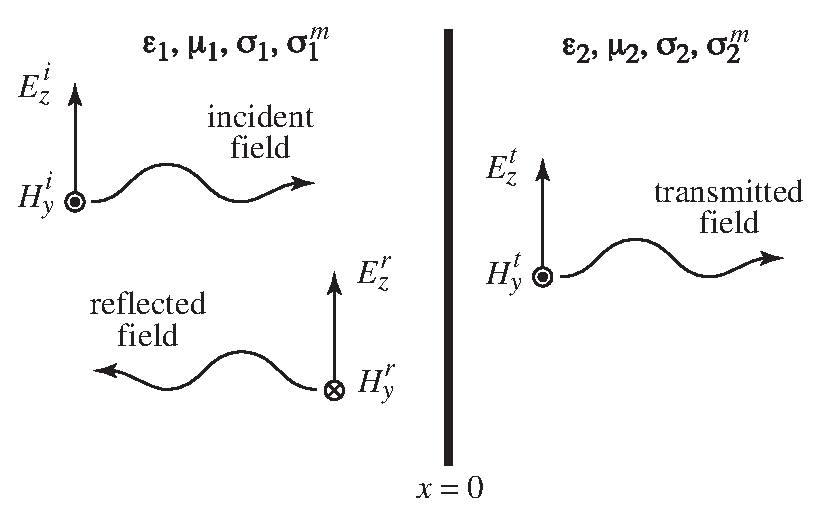
\epsfig{width=3.75in,%
            file=Figures/Fdtd-dimensionless/planar-interface.eps}
  \end{center}
  \caption{Planar interface between two media.  The interface is at
 $x=0$ and a wave is incident on the interface from the left.  When the
 impedances of the two media are not matched, a reflected wave must
 exist in order to satisfy the boundary conditions.}
  \label{fig:planarInterface}
\end{figure}
In the frequency domain, the incident, reflected, and transmitted
fields are given by
\begin{eqnarray}
  \hE_z^i(x) \!&=&\! \hE_{a1}^+ e^{-\hgamma_1 x} 
    \qquad \mbox{\hspace{.92in}incident},\\
  \hE_z^r(x) \!&=&\! \hE_{a1}^- e^{+\hgamma_1 x} =
                   \hG \hE_{a1}^+ e^{+\hgamma_1 x} \qquad \mbox{reflected},\\
  \hE_z^t(x) \!&=&\! \hE_{a2}^+ e^{-\hgamma_2 x} =
                   \hT \hE_{a1}^+ e^{-\hgamma_2 x} \qquad \mbox{transmitted},
\end{eqnarray}
where $\hG$ is the reflection coefficient, $\hT$ is the transmission
coefficient, and $\hgamma_n$ is the propagation constant given by
$j\omega\sqrt{\mu_n(1-j\sigma^m_n/\omega\mu_n)
  \epsilon_n(1-j\sigma_n/\omega\epsilon_n)}$ where the $n$ indicates
the medium and $\sigma^m$ is the magnetic conductivity.  The amplitude
of the incident field $\hE_{a1}^+$ is, in general, complex and a
function of frequency.  By definition $\hG$ and $\hT$ are
\begin{eqnarray}
  \hG &=& \left.\frac{\hE_z^r(x)}{\hE_z^i(x)}\right|_{x=0} =
              \frac{\hE_{a1}^-}{\hE_{a1}^+}, \\
       \hT &=& \left.\frac{\hE_z^t(x)}{\hE_z^i(x)}\right|_{x=0} = 
              \frac{\hE_{a2}^+}{\hE_{a1}^+}.
\end{eqnarray}
The fact that these are defined at $x=0$ is important.

The magnetic field is related to the electric field by
\begin{eqnarray}
  \hH_y^i(x) &=& -\frac{1}{\heta_1}\hE_z^i(x), \\ 
  \hH_y^r(x) &=& \frac{1}{\heta_1}\hE_z^r(x), \\ 
  \hH_y^t(x) &=& -\frac{1}{\heta_2}\hE_z^t(x),
\end{eqnarray}
where the characteristic impedance $\heta_n$ is given by
$\sqrt{\mu_n(1-j\sigma^m_n/\omega\mu_n)/
  \epsilon_n(1-j\sigma_n/\omega\epsilon_n)}$.  Since the magnetic and
electric fields are purely tangential to the planar interface, the sum
of the incident and reflected field at $x=0$ must equal the
transmitted field at the same point.  Matching the boundary condition
on the electric field yields
\begin{equation}
  1 + \hG = \hT,
  \label{eq:matchingFields}
\end{equation}
while matching the boundary conditions on the magnetic field produces
\begin{equation}
 \frac{1}{\heta_1}(1 - \hG) = \frac{1}{\heta_2}\hT.
\end{equation}
Solving these for $\hT$ yields
\begin{equation}
  \hT = \frac{2\heta_2}{\heta_1+\heta_2}.
  \label{eq:transCoefSpectral}
\end{equation}
Using this in \refeq{eq:matchingFields} the reflection coefficient is
found to be
\begin{equation}
  \hG = \frac{\heta_2-\heta_1}{\heta_2+\heta_1}.
  \label{eq:refCoefSpectral}
\end{equation}

\subsection{Measuring the Transmission Coefficient Using FDTD
\label{sec:measureTrans}}

Now consider two FDTD simulations.  The first simulation will be used
to record the incident field.  In this simulation the computational
domain is homogeneous and the material properties correspond to that
of the first medium.  The field is recorded at some observation point
$x_1$.  Since nothing is present to interfere with the incident field,
the recorded field will be simply the incident field at this location,
i.e, $E_z^i(x_1,t)$.  In the second simulation, the second medium is
present.  We record the fields at the same observation point but we
ensure the point was chosen such that it is located in the second
medium (i.e., the interface is to the left of the observation point).
Performing an FDTD simulation in this case yields the transmitted
field $E_z^t(x_1,t)$.  The goal now is to obtain the transmission
coefficient using the temporal recordings of the field obtained from
these two simulations.

{\em Note} that in this section we will not distinguish between the
way in which field propagate in the continuous world and the way in
which they propagate in the FDTD grid.  In
Chap.\ \ref{chap:dispersion} we will discuss in some detail how these
differ.

One cannot use $E_z^t(x_1,t)/E_z^i(x_1,t)$ to obtain the transmission
coefficient.  The transmission coefficient is inherently a
frequency-domain concept and currently we have time-domain signals.
The division of these temporal signals is essentially meaningless
(e.g., the result is undefined when the incident signal is zero).

The incident and transmitted fields must be converted to the frequency
domain using a Fourier transform.  Thus one obtains
\begin{eqnarray}
 \hE_z^i(x_1) &=& {\cal F}\left(E_z^i(x_1,t)\right), \\
 \hE_z^t(x_1) &=&  {\cal F}\left(E_z^t(x_1,t)\right),
\end{eqnarray} 
where ${\cal F}$ indicates the Fourier transform.  The division of
these two functions {\em is} meaningful---at least at all frequencies
where $\hE_z^i(x_1)$ is non-zero.  (At frequencies where
$\hE_z^i(x_1)$ is zero, there is no incident spectral energy and hence
one cannot obtain the transmitted field at those particular
frequencies.  In practice it is relatively easy to introduce energy
into an FDTD grid that spans a broad range of frequencies.)

Since the observation point was not specified to be on the boundary,
the ratio of these field fields is
\begin{equation}
  \frac{\hE_z^t(x_1)}{\hE_z^i(x_1)} =
  \frac{\hE_{a2}^+e^{-\hgamma_2 x_1}}{\hE_{a1}^+e^{-\hgamma_1 x_1}} =
  \frac{\hE_{a2}^+}{\hE_{a1}^+}e^{(\hgamma_1-\hgamma_2) x_1} =
  \hT e^{(\hgamma_1-\hgamma_2) x_1}.
\end{equation}
Solving this for $\hT$ yields
\begin{equation}
  \hT(\omega) = e^{(\hgamma_2-\hgamma_1) x_1}
  \frac{\hE_z^t(x_1)}{\hE_z^i(x_1)}.
  \label{eq:transCoefShifted}
\end{equation}

To demonstrate how the transmission coefficient can be
reconstructed from FDTD simulations, let us consider an example where
the first medium is free space and the second one has a relative
permittivity $\epsilon_r$ of $9$.  In this case
$\hgamma_1=j\omega\sqrt{\mu_0\epsilon_0}=j\beta_0$ and
$\hgamma_2=j\omega\sqrt{\mu_0 9\epsilon_0}=j3\beta_0$.
Therefore \refeq{eq:transCoefShifted} becomes
\begin{equation}
  \hT(\omega) = e^{j(3\beta_0-\beta_0) x_1}
  \frac{\hE_z^t(x_1)}{\hE_z^i(x_1)}
  = e^{j2\beta_0 x_1}
  \frac{\hE_z^t(x_1)}{\hE_z^i(x_1)}.
\end{equation}
The terms in the exponent can be written
\begin{equation}
  2\beta_0 x_1 = 2\frac{2\pi}{\lambda}x_1 = 
  \frac{4\pi}{\ppw\Delx}N_1\Delx =
  \frac{4\pi}{\ppw}N_1
  \label{eq:transExponent}
\end{equation}
where $N_1$ is the number of spatial steps between the interface and
the observation point at $x_1$ and, as was discussed in Chap.\
\ref{chap:dimensionless}, $\ppw$ is the number of spatial steps per a
free-space wavelength of $\lambda$.

The continuous-world transmission coefficient can be calculated quite
easily from \refeq{eq:transCoefSpectral} and this provides a reference
solution.  Ideally the FDTD simulation would yield this same value for
all frequencies.  For this particular example the characteristic
impedance of the first medium is $\heta_1=\eta_0$ while for the second
medium it is $\heta_2=\eta_0/3$.  Thus the transmission coefficient
is
\begin{equation}
  \hT_{\mbox{\scriptsize exact}} = \frac{2\eta_0/3}{\eta_0+\eta_0/3} = 1/2.
  \label{eq:transExact}
\end{equation}
Note that this is a real number and independent of frequency (so the
tilde on $T$ is somewhat misleading).

For the FDTD simulations, let us record the field 80 spatial steps
away from the interface, i.e., $N_1=80$, and run the simulation for
8192 time steps, i.e., $N_T=8192$.  The simulation is run at the
Courant limit $S_c=1$.  The source is a Ricker wavelet discretized so
that the peak spectral content exists at 50 points per wavelength
($N_P=50$).  From Sec.\
\ref{sec:fftMapping}, recall the relationship between the points per
wavelength $\ppw$ and frequency index $N_{\mathrm{freq}}$ which is
repeated below:
\begin{equation}
  N_{\mathrm{freq}} = \frac{N_T}{\ppw} S_c.
\end{equation}
With a Courant number of unity and 8192 time steps, the points per
wavelength for any given frequency (or spectral index) is given by
\begin{equation}
  \ppw = \frac{8192}{N_{\mathrm{freq}}}.
\end{equation}
Combining this with \refeq{eq:transCoefShifted} and
\refeq{eq:transExponent} yields
\begin{equation}
  \hT_{\mbox{\scriptsize FDTD}}
  = e^{j\left(\frac{4\pi N_1N_{\mathrm{freq}}}{8192}\right)}
  \frac{\hE_z^t(x_1)}{\hE_z^i(x_1)}.
  \label{eq:transFDTD}
\end{equation}

Ideally \refeq{eq:transExact} and \refeq{eq:transFDTD} will agree at
all frequencies.  To see if that is the case, Fig.\
\ref{fig:incTransFields} shows three plots related to the incident and
transmitted fields.  Figure \ref{fig:incTransFields}(a) shows the
first 500 time steps of the temporal signals recorded at the
observation point both with and without the interface present
(i.e., the transmitted and incident fields, respectively).  Figure
\ref{fig:incTransFields}(b) shows the magnitude of the Fourier
transforms of the incident and transmitted fields for the first 500
frequencies.  Since a Ricker wavelet was used, the spectra are
essentially in accordance with the discussion of Sec.\
\ref{sec:ricker}.  There is no spectral energy at dc and the spectral
content exponentially approaches zero at high frequencies.

\begin{figure}
  \begin{center}
   \epsfig{width=5.4in,file=Code/Fdtd-spectral/fields.eps}
  \end{center}

  \caption{(a) Time-domain fields at the observation point both with
   and the without the interface present.  The field without the
   interface is the incident field and the one with the interface is
   the transmitted field.  (b) Magnitude of the Fourier transforms of
   the incident and transmitted fields.  The transforms are plotted
   versus the frequency index $N_{\mathrm{freq}}$.  It can be seen that
   the fields do not have much spectral content near dc nor at high
   frequencies.  (c) Magnitude of the transmitted field normalized by
   the incident field versus the frequency index.  Ideally this would
   be $1/2$ for all frequencies.  Errors are clearly evident when the
   spectral content of the incident field is small.}
   \label{fig:incTransFields}
\end{figure}

Figure \ref{fig:incTransFields}(c) plots the magnitude of the ratio of
the transmitted and incident field as a function of frequency.
Ideally this would be $1/2$ for all frequencies.  Note the rather
small vertical scale of the plot.  Near dc the normalized transmitted
field differs rather significantly from the ideal value, but this is
in a region where the results should not be trusted because there is
not enough incident energy at these frequencies.  At the higher
frequencies some oscillations are present.  The normalized field
generally remains within two percent of the ideal value over this
range of frequencies.

Figure \ref{fig:transCoefVsFreq}(a) provides the same information as
Fig.\ \ref{fig:incTransFields}(c) except now the result is plotted
versus the discretization $\ppw$.  In this figure dc is off the scale
to the right (since in theory dc has an infinite number of points per
wavelength).  As the frequency goes up, the wavelength gets shorter
and hence the number of points per wavelength decreases.  Thus high
frequencies are to the left and low frequencies are to the right.  The
highest frequency in this plot corresponds to an $N_{\mathrm{freq}}$
of $500$.  In terms of the discretization, this is
$N_\lambda=N_T/N_{\mathrm{freq}}=16.384$.  This may not seem like a
particularly coarse discretization, but one needs to keep in mind that
this is the discretization in frees pace.  Within the dielectric, which
here has $\epsilon_r=9$, the wavelength is three times smaller and
hence within the dielectric the fields are only discretized at
approximately five points per wavelength (which is considered a very
coarse discretization).  From this figure it is clear that the FDTD
simulations provide results which are close to the ideal over a fairly
broad range of frequencies.

\begin{figure}
  \begin{center}
   \epsfig{width=5.4in,file=Code/Fdtd-spectral/trans-coef.eps}
  \end{center}
  \caption{(a) The magnitude of the normalized transmitted field as a
    function of the (free space) discretization $N_\lambda$.  Ideally
    this would be $1/2$ for all discretizations. (b) Real and
    imaginary part of the transmission coefficient transformed back to
    the interface $x=0$ versus discretization.  Ideally the real part
    would be $1/2$ and the imaginary part would be zero for all
    discretization.  For these plots the observation point was $80$
    cells from the interface ($N_1 = 80$).
   \label{fig:transCoefVsFreq}}
\end{figure}

Figure \ref{fig:transCoefVsFreq}(b) shows the real and imaginary part of
the reflection coefficient, i.e., $\hT_{\mbox{\scriptsize FDTD}}$
defined in \refeq{eq:transFDTD}, as a function of the discretization.
Ideally the imaginary part would be zero and the real part would be
$1/2$.  As can be seen, although the magnitude of the transmission
coefficient is nearly $1/2$ over the entire spectrum, the phase differs
rather significantly as the discretization decreases (i.e., the
frequency increases).  

The Matlab code used to generate Fig.\ \ref{fig:incTransFields} is
shown in Program \ref{pro:transformFields} while the code which
generated Fig.\ \ref{fig:transCoefVsFreq} is given in Program
\ref{pro:transCoefficient}.  It is assumed the incident field from the
FDTD simulation is recorded to a file named {\tt inc-8192} while the
transmitted field, i.e., the field when the dielectric is present, is
recorded in {\tt die-8192}.  The code in Program
\ref{pro:transformFields} has to be run prior to that of 
\ref{pro:transCoefficient} in order to load and initialize the data.

Let us now consider the same scenario but let the observation point be
four steps away from the boundary instead of $80$, i.e., $N_1=4$.
Following the previous steps, the incident and transmitted fields are
recorded, their transforms are taken, then divided, and finally the
phase is adjusted to obtain the transmission coefficient.  The result
for this observation point is shown in Fig.\
\ref{fig:transCoefVsFreqX4}.  The real and imaginary parts stay closer
to the ideal values over a larger range of frequencies than when the
observation point was $80$ cells from the boundary.  The fact that the
quality of the results are frequency sensitive as well as sensitive to
the observation point is a consequence of numeric dispersion in the
FDTD grid, i.e., different frequencies propagate at different speeds.
(This is the subject of Chap.\ \ref{chap:dispersion}.)
\begin{figure}
  \begin{center}
   \epsfig{width=5.4in,file=Code/Fdtd-spectral/trans-coef-x4.eps}
  \end{center}

  \caption{Real and imaginary part of the transmission coefficient
    transformed back to the interface $x=0$ versus discretization.
    Ideally the real part would be $1/2$ and the imaginary part would
    be zero for all discretization.  The observation point was four
    cells from the interface ($N_1 = 4$).}
   \label{fig:transCoefVsFreqX4}
\end{figure}

\begin{program}
Matlab session used to generate Fig.\ \ref{fig:incTransFields}.
 \label{pro:transformFields}
\codemiddle
\begin{lstlisting}[language=Matlab]
incTime = dlmread('inc-8192'); % incident field file
dieTime = dlmread('die-8192'); % transmitted field file

inc = fft(incTime);  % take Fourier transforms
die = fft(dieTime);

nSteps = length(incTime);  % number of time steps
freqMin = 1;    % minimun frequency index of interest
freqMax = 500;  % maximum frequency of interest
freqIndex = freqMin:freqMax; % range of frequencies of interest
% correct for offset of 1 in matlab's indexing
freqSlice = freqIndex + 1;
courantNumber = 1;
% points per wavelength for freqencies of interest
nLambda = nSteps ./ freqIndex * courantNumber;
clf
subplot(3, 1, 1)
hold on
plot(incTime(freqSlice), '-.');
plot(dieTime(freqSlice));
legend('Incident field', 'Transmitted field');
xlabel('Temporal Index');
ylabel('{\it E_z}[{\it x}_1,{\it t}] V/m');
title('(a) Temporal Fields');

subplot(3,1,2)
hold on
plot(freqIndex, abs(inc(freqSlice)), '-.');
plot(freqIndex, abs(die(freqSlice)));
legend('Incident field', 'Transmitted field');
xlabel('Frequency Index');
ylabel('|{\it E_z}[{\it x}_1,\omega]|');
title('(b) Transform vs. Frequency Index');
hold off

subplot(3, 1, 3)
hold on
plot(freqIndex, abs(die(freqSlice) ./ inc(freqSlice)));
xlabel('Frequency Index');
ylabel('|{\it E^t_z}[{\it x}_1,\omega]/...
                          {\it E^i_z}[{\it x}_1,\omega]|');
title('(c) Normalized Transmitted Field vs. Frequency Index');
hold off
\end{lstlisting}
\end{program}

\begin{program}
Matlab session used to generate Fig.\
\ref{fig:transCoefVsFreq}.  The commands shown in Program
\ref{pro:transformFields} would have to be run prior to these
commands in order to read the data, generate the Fourier transforms, etc.
 \label{pro:transCoefficient}
\codemiddle
\begin{lstlisting}[language=Matlab]
clf

subplot(2, 1, 1)
hold on
plot(nLambda, abs(die(freqSlice) ./ inc(freqSlice)));
xlabel('Points per Wavelength');
ylabel('|{\it E^t_z}[{\it x}_1,\omega]/...
                          {\it E^i_z}[{\it x}_1,\omega]|');
title('(a) Normalized Transmitted Field vs. Discretization');
axis([0 300 0 1])
hold off

% Array obtained from exp() must be transposed to make arrays
% conformal.  Simply using ' (a prime) for trasposition will yield
% the conjugate transpose.  Instead, use .' (dot-prime) to get
% transposition without conjugation.
subplot(2, 1, 2)
hold on
plot(nLambda, real(exp(j*pi*freqIndex/25.6).' .* ...
                   die(freqSlice) ./ inc(freqSlice)));
plot(nLambda, imag(exp(j*pi*freqIndex/25.6).' .* ...
                   die(freqSlice) ./ inc(freqSlice)), '-.');
xlabel('Points per Wavelength');
ylabel('Transmission Coefficient, {\it T}(\omega)');
title('(b) Real and Imaginary Part of Transmission Coefficient');
legend('Real part', 'Imaginary part');
axis([0 300 -1 1])
grid on
hold off
\end{lstlisting}
\end{program}

Although we have only considered the transmission coefficient in this
example, the reflection coefficient could be obtained in a similar
fashion.  We have intentionally considered a very simple problem in
order to be able to compare easily the FDTD solution to the exact
solution.  However one should keep in mind that the FDTD method could
be used to analyze the reflection or transmission coefficient for a
much more complicated scenario, e.g., one in which the material
properties varied continuously, and perhaps quite erratically (with
some discontinuities present), over the transition from one half-space
to the next.  Provided a sufficiently small spatial step-size was
used, the FDTD method can solve this problem with essentially no more
effort than was used to model the abrupt interface.  However, to
obtain the exact solution, one may have to work much harder.

\chapter[Differential-Equation Based ABC's]{Differential-Equation
Based Absorbing Boundary Conditions \label{chap:abc}}

%\setcounter{page}{1}

\renewcommand{\thefootnote}{\fnsymbol{footnote}}
\footnotetext{Lecture notes by John Schneider.  {\tt
fdtd-abc.tex}}

\section{Introduction}

A simple absorbing boundary condition (ABC) was used in Chap.\
\ref{chap:fdtdIntro} to terminate the grid.  It relied upon the fact
that the fields were propagating in one dimension and the speed of
propagation was such that the fields moved one spatial step for every
time step, i.e., the Courant number was unity.  The node on the
boundary was updated using the value of the adjacent interior node
from the previous time step.  However, when a dielectric was
introduced, and the local speed of propagation was no longer equal to
$c$, this ABC ceased to work properly.  One would also find in higher
dimensions that this simple ABC would not work even in free space.
This is because the Courant number cannot be unity in higher
dimensions and this ABC does not account for fields which may be
obliquely incident on the edge of the grid.  The goal now is to find a
more general technique to terminate the grid.

Although the ABC we will discuss here is not considered
state-of-the-art, it provides a relatively simple way to terminate the
grid that is more than adequate in many circumstances.  Additionally,
some of the mathematical tools we will develop in this chapter can be
used in the analysis of a wide range of FDTD-related topics.

\section{The Advection Equation \label{sec:advection}}

The wave equation that governs the propagation of the electric field
in one dimension is
\begin{eqnarray}
  \frac{\partial^2 E_z}{\partial x^2}
  - \mu\epsilon \frac{\partial^2 E_z}{\partial t^2} &=& 0,
  \label{eq:waveEqOneD}
 \\
  \left(\frac{\partial^2}{\partial x^2}
  - \mu\epsilon \frac{\partial^2}{\partial t^2}\right) E_z &=& 0.
\end{eqnarray}
The second form represents the equation in terms of an operator
operating on $E_z$ where the operator is enclosed in parentheses.
This operator can be factored into the product of two operators and is
equivalent to
\begin{equation}
  \left(\frac{\partial }{\partial x}
  -\sqrt{\mu\epsilon} \frac{\partial }{\partial t}\right)
  \left(\frac{\partial }{\partial x}
  +\sqrt{\mu\epsilon} \frac{\partial }{\partial t}\right)
  E_z
  = 0.
  \label{eq:factoredWaveEq}
\end{equation}
Note that it does not matter which operator in
\refeq{eq:factoredWaveEq} is written first.  They commute and will
always ultimately yield \refeq{eq:waveEqOneD}.  If either of these
operators acting individually on the field yields zero, the wave
equation is automatically satisfied.  Thus an $E_z$ that satisfies
either of the following equations will also be a solution to the wave
equation:
\begin{eqnarray}
  \frac{\partial E_z}{\partial x}
  - \sqrt{\mu\epsilon} \frac{\partial E_z}{\partial t} &=& 0, 
  \label{eq:advection}
  \\
  \frac{\partial E_z}{\partial x}
  + \sqrt{\mu\epsilon} \frac{\partial E_z}{\partial t}
  &=& 0.
  \label{eq:advectionI}
\end{eqnarray}
These equations are sometimes called advection equations.  Note that a
solution to the wave equation will not simultaneously satisfy both
these advection equations (except in trivial cases).  It may satisfy
one or the other but not both.  In fact, fields may be a solution to
the wave equation and yet satisfy neither of the advection
equations.\footnote{As an example, consider $E_z(x,t) = \cos(\omega
  t)\sin(\beta x)$ where $\beta = \omega\sqrt{\mu\epsilon}$.}

A solution to \refeq{eq:advection} is
$E_z(t+\sqrt{\mu\epsilon}x)$, i.e., a wave traveling in the negative
$x$ direction.  The proof proceeds along the same lines
as the proof given in Sec.\ \ref{sec:waveEq}.  Equate the argument
with $\xi$ so that
\begin{equation}
  \xi = t+\sqrt{\mu\epsilon}x.
\end{equation}
Derivatives of the argument with respect to time or space are given by
\begin{equation}
  \frac{\partial\xi}{\partial t}=1  \quad \mbox{and} \quad
  \frac{\partial\xi}{\partial x}=\sqrt{\mu\epsilon}.
\end{equation}
Thus,
\begin{eqnarray}
 \frac{\partial E_z}{\partial x} \!&=&\!
    \frac{\partial E_z}{\partial \xi}\frac{\partial \xi}{\partial x} = 
    \sqrt{\mu\epsilon}\frac{\partial E_z}{\partial \xi}, 
 \label{eq:advecProof}
  \\
 \frac{\partial E_z}{\partial t} \!&=&\!
    \frac{\partial E_z}{\partial \xi}\frac{\partial \xi}{\partial t} = 
    \frac{\partial E_z}{\partial \xi}.
 \label{eq:advecProofI}
\end{eqnarray}
Plugging the right-hand sides of \refeq{eq:advecProof} and
\refeq{eq:advecProofI} into \refeq{eq:advection} yields zero and the
equation is satisfied.  It is worth mentioning that although
$E_z(t+\sqrt{\mu\epsilon}x)$ is a solution to 
\refeq{eq:advection}, it is not a solution to \refeq{eq:advectionI}.

\section{Terminating the Grid}

Let us now consider how an advection equation can be used to provide
an update equation for a node at the end of the computational domain.
Let the node $\fdtd{E_z}{0}{q+1}$ be the node on the boundary for
which an update equation is sought.  Since interior nodes can be
updated before the boundary node, assume that all the adjacent nodes
in space-time are known, i.e., $\fdtd{E_z}{1}{q+1}$,
$\fdtd{E_z}{0}{q}$, and $\fdtd{E_z}{1}{q}$ are known.  At the left end
of the grid, the fields should only be traveling to the left.  Thus
the fields satisfy the advection equation \refeq{eq:advection}.  The
finite-difference approximation of this equation provides the
necessary update equation, but the way to discretize the equation is
not entirely obvious.  A stable ABC will result if the equation is
expanded about the space-time point $(\Delx/2,(q+1/2)\Delt)$.  This
point is shown in Fig.\ \ref{fig:advectionABC}.

\begin{figure}
  \begin{center}
  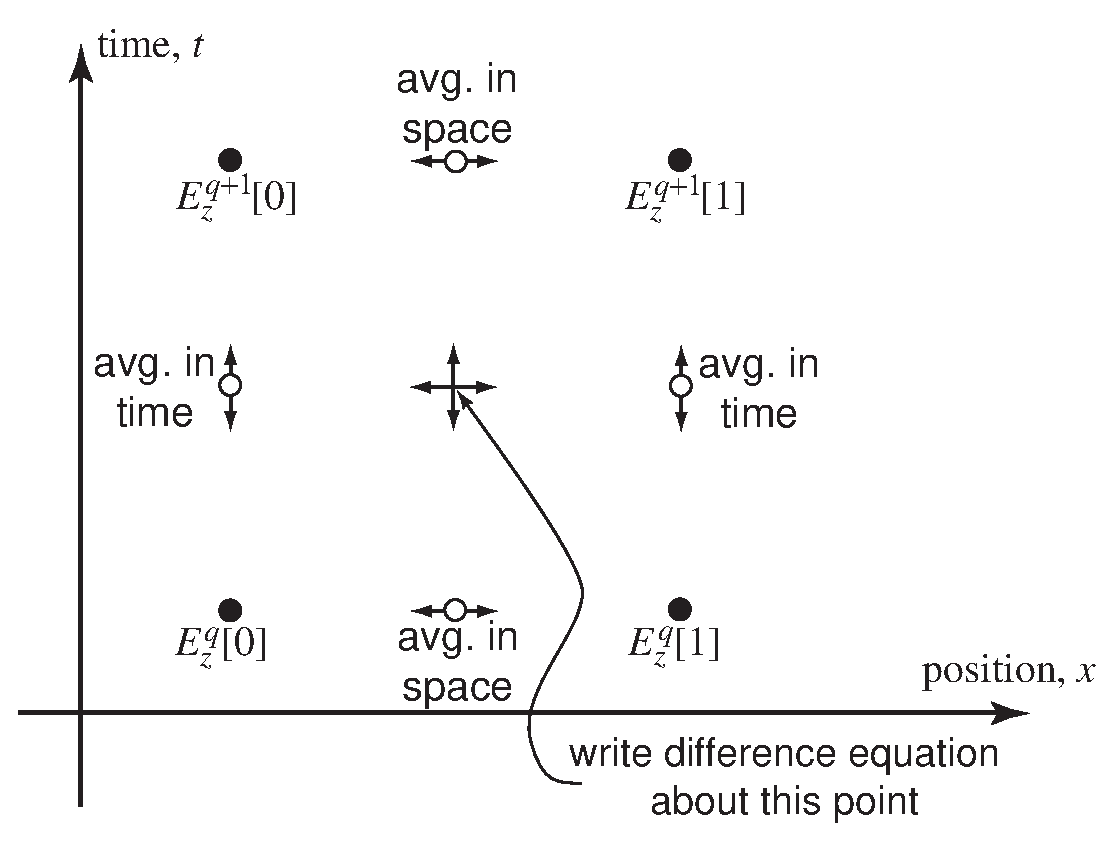
\epsfig{width=4.in,file=Figures/Fdtd-abc/abc-first-order.eps}
  \end{center}
  \caption{Space-time in the neighborhood of the left end of the grid.
  Only the electric fields are shown.  The open circles indicated
  where an electric field is needed for the advection equation.  Since
  there are none there, averaging is used to approximate the field at
  those points.}  \label{fig:advectionABC}
\end{figure}

At first it seems like this in an unacceptable point about which to
expand the advection equation since moving forward or backward in time
or space a half step does not correspond to the location of an
electric field point.  To fix this, the electric field will be averaged
in either time or space to obtain an estimate of the value at the
desired location in space-time.  For example, to obtain an
approximation of $\fdtd{E_z}{1/2}{q+1}$, the average
$(\fdtd{E_z}{0}{q+1}+\fdtd{E_z}{1}{q+1})/2$, would be used.
Similarly, an approximation of $\fdtd{E_z}{1/2}{q}$ would be
$(\fdtd{E_z}{0}{q}+\fdtd{E_z}{1}{q})/2$.  Therefore the temporal
derivative would be approximated with the following finite difference:
\begin{equation}
  \left. \sqrt{\mu\epsilon}
    \frac{\partial E_z}{\partial t}\right|_{\Delx/2,(q+1/2)\Delt}
  \approx
    \sqrt{\mu\epsilon}
    \frac{
     \frac{\fdtd{E_z}{0}{q+1}+\fdtd{E_z}{1}{q+1}}{2} -
     \frac{\fdtd{E_z}{0}{q}+\fdtd{E_z}{1}{q}}{2}
    }{\Delt}
   \label{eq:tDiffSpaceAvg}
\end{equation}

Averaging in time is used to obtain the fields at the proper locations
for the spatial finite difference.  The resulting finite difference is
\begin{equation}
  \left.
    \frac{\partial E_z}{\partial x}\right|_{\Delx/2,(q+1/2)\Delt}
  \approx
    \frac{
     \frac{\fdtd{E_z}{1}{q+1}+\fdtd{E_z}{1}{q}}{2} -
     \frac{\fdtd{E_z}{0}{q+1}+\fdtd{E_z}{0}{q}}{2}
    }{\Delx}
  \label{eq:xDiffTimeAvg}
\end{equation}
Combining \refeq{eq:tDiffSpaceAvg} and \refeq{eq:xDiffTimeAvg} yields
the finite-difference form of the advection equation
\begin{equation}
   \frac{
    \frac{\fdtd{E_z}{1}{q+1}+\fdtd{E_z}{1}{q}}{2} -
    \frac{\fdtd{E_z}{0}{q+1}+\fdtd{E_z}{0}{q}}{2}
   }{\Delx}
  -
   \sqrt{\mu\epsilon}
   \frac{
    \frac{\fdtd{E_z}{0}{q+1}+\fdtd{E_z}{1}{q+1}}{2} -
    \frac{\fdtd{E_z}{0}{q}+\fdtd{E_z}{1}{q}}{2}
   }{\Delt}
 = 0.
\end{equation}
Letting $\sqrt{\mu\epsilon}=\sqrt{\mu_r\epsilon_r}/c$ and
solving for $\fdtd{E_z}{0}{q+1}$ yields
\begin{equation}
  \fdtd{E_z}{0}{q+1} = \fdtd{E_z}{1}{q} +
    \frac{\frac{S_c}{\sqrt{\mu_r\epsilon_r}}-1}
         {\frac{S_c}{\sqrt{\mu_r\epsilon_r}}+1}
    \left(\fdtd{E_z}{1}{q+1}-\fdtd{E_z}{0}{q}\right)
  \label{eq:firstOrderABC}
\end{equation}
where $S_c$ is the Courant number $c\Delt/\Delx$.  Equation
\refeq{eq:firstOrderABC} provides a first-order absorbing boundary
condition that updates the field on the boundary using the values of
past and interior fields.  This is known as a first-order ABC because
it was constructed from a first-order differential equation.
Note that when $S_c/\sqrt{\mu_r\epsilon_r}$
is unity, which would be the case of free space and a unit Courant
number, \refeq{eq:firstOrderABC} reduces to $\fdtd{E_z}{0}{q+1} =
\fdtd{E_z}{1}{q}$ which is the simple grid-termination
technique presented in Sec.\ \ref{sec:terminate}.

At the other end of the grid, i.e., at the right end of the grid, an
equation that is nearly identical to \refeq{eq:firstOrderABC}
pertains.  Equation \refeq{eq:advectionI} would be expanded in the
neighborhood of the last node of the grid.  Although
\refeq{eq:advection} and \refeq{eq:advectionI} differ in the sign of
one term, when \refeq{eq:advectionI} is applied it is ``looking'' in
the negative $x$ direction.  That effectively cancels the sign change.
Hence the update equation for the last node in the grid, which is
identified here as $\fdtd{E_z}{M}{q+1}$, would be
\begin{equation}
  \fdtd{E_z}{M}{q+1} = \fdtd{E_z}{M-1}{q} +
    \frac{\frac{S_c}{\sqrt{\mu_r\epsilon_r}}-1}
         {\frac{S_c}{\sqrt{\mu_r\epsilon_r}}+1}
    \left(\fdtd{E_z}{M-1}{q+1}-\fdtd{E_z}{M}{q}\right).
  \label{eq:firstOrderABCI}
\end{equation}

Recall that for a lossless medium, the coefficient in the
electric-field update equation that multiplied the magnetic fields was
$\Delt/\epsilon\Delx$ and this could be expressed as
$S_c\eta_0/\epsilon_r$.  On the other hand, the coefficient in the
magnetic-field update equation that multiplied the electric fields was
$\Delt/\mu\Delx$ and this could be expressed as $S_c/\eta_0\mu_r$.
Therefore, taking the product of these two coefficients and taking the
square root yields
\begin{equation}
  \left(\frac{\Delt}{\epsilon\Delx}
        \frac{\Delt}{\mu\Delx}\right)^{1/2} =
        \frac{S_c}{\sqrt{\mu_r\epsilon_r}}.
  \label{eq:abcCoefFirstOrder}
\end{equation}
Note that this is the term that appears in \refeq{eq:firstOrderABC}
and \refeq{eq:firstOrderABCI}.
Thus by knowing the update coefficients that pertain at the ends of
the grid, one can calculate the coefficients that appear in the ABC.

\section{Implementation of a First-Order ABC}

Program \ref{pro:1Ddielectric} modeled two half spaces: free space and
a dielectric.  That program was written as a ``monolithic'' program
with a {\tt main()} function in which all the calculations were
performed.  For that program we did not have a suitable way to
terminate the grid within the dielectric.  Let us re-implement that
program but use the modular design that was discussed in Chap.\
\ref{chap:fdtdImproved} and use the ABC presented in the previous
section.  

Recalling the modular design used to model a lossy layer that was
discussed in Sec.\ \ref{sec:improveThree}, we saw that the ABC was so
simple there was no need to do any initialization of the ABC.
Nevertheless, recalling the code shown in Program \ref{pro:improved3},
an ABC initialization function was called, but it merely returned
without doing anything.  Now that we wish to implement a first-order
ABC, the ABC initialization function actually needs to perform some
calculations: it will calculate any of the constants associated with
the ABC.  

Naturally, the code associated with the various
``blocks'' in our modular design will need to change from what was
presented in Sec.\ \ref{sec:improveThree}.  However, the overall
framework remains essentially the same!  The arrangement of files
associated with our model of halfspace that uses a first-order ABC
is shown in Fig.\ \ref{fig:firstOrderAbcFiles}.  Note that this figure
and Fig.\ \ref{fig:improvedFiles} are nearly the same.  They both have
the same layout.  All the functions have the same name, but the
implementation of some of those functions have changed.  Note that the
file names have changed for the files containing the {\tt main()}
function, the {\tt gridInit()} function, and the {\tt abc()} and {\tt
  abcInit()} function.  
\begin{figure}
  \begin{center}
  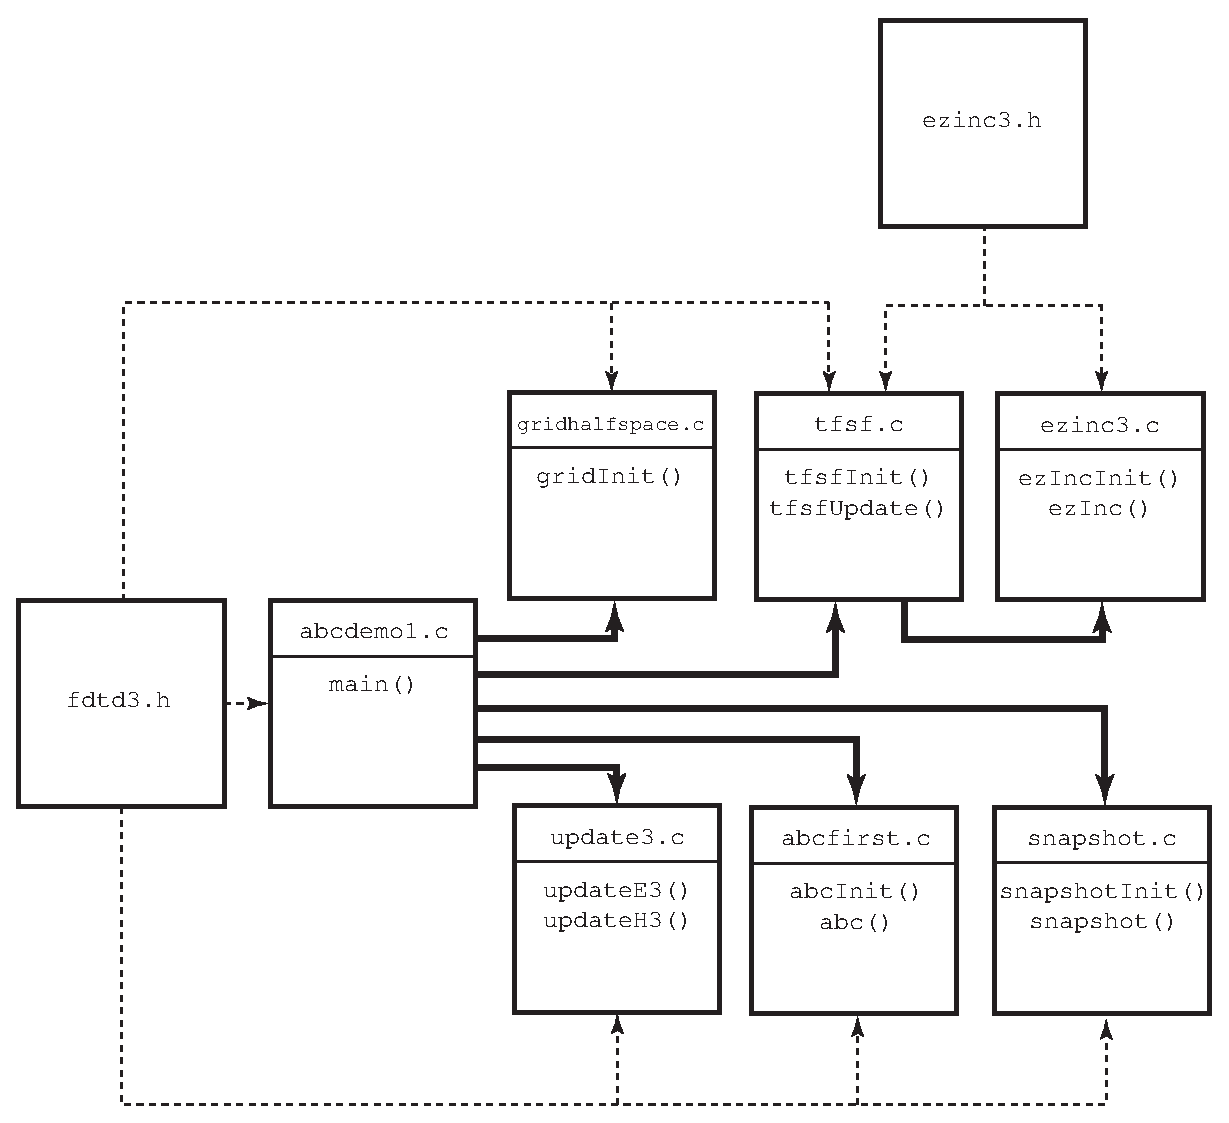
\epsfig{width=6.3in,file=Figures/Fdtd-abc/abcdemo1-files.eps}
\end{center} \caption{Files associated with the modular implementation
  of a simulation of a dielectric half space.  Since a first-order ABC
  is now being used, some of these files differ from those of Fig.\
  \ref{fig:improvedFiles}.  Nevertheless, the overall structure of the
  program is unchanged and all the function names are the same as
  before.}
  \label{fig:firstOrderAbcFiles}
\end{figure}


The code associated with the TFSF boundary, the snapshots, the source
function, and the update equations are all unchanged from that which
was described in Chap.\ \ref{chap:fdtdImproved}.  The grid
initialization function {\tt gridInit()} constructs a half-space
dielectric consistent with Program \ref{pro:1Ddielectric}.  The code
is shown in Program \ref{pro:gridInit1DhalfSpace}.

\begin{program} {\tt gridhalfspace.c}: Function to initialize the {\tt
    Grid} such that there are two half-spaces: free space to the left
  and a dielectric with $\epsilon_r=9$ to the right.
\label{pro:gridInit1DhalfSpace}
\codemiddle
\begin{lstlisting}
/* Function to initialize the Grid structure. */

#include "fdtd3.h"

#define EPSR 9.0

void gridInit(Grid *g) {
  double imp0 = 377.0;
  int mm;

  SizeX = 200;   // size of domain
  MaxTime = 450; // duration of simulation
  Cdtds = 1.0;   // Courant number

  ALLOC_1D(g->ez,   SizeX, double);
  ALLOC_1D(g->ceze, SizeX, double);
  ALLOC_1D(g->cezh, SizeX, double);
  ALLOC_1D(g->hy,   SizeX - 1, double);
  ALLOC_1D(g->chyh, SizeX - 1, double);
  ALLOC_1D(g->chye, SizeX - 1, double);
  
  /* set electric-field update coefficients */
  for (mm = 0; mm < SizeX; mm++)
    if (mm < 100) {
      Ceze(mm) = 1.0;
      Cezh(mm) = imp0;
    } else {
      Ceze(mm) = 1.0;
      Cezh(mm) = imp0 / EPSR;
    }

  /* set magnetic-field update coefficients */
  for (mm = 0; mm < SizeX - 1; mm++) {
    Chyh(mm) = 1.0;
    Chye(mm) = 1.0 / imp0;
  }

  return;
}
\end{lstlisting}
\end{program}

The contents of the file {\tt abcdemo1.c} are shown in Program
\ref{pro:abcdemo1}.  The difference between {\tt abcdemo1.c} and {\tt
  improved3.c}, which is given in Program \ref{pro:improved3}, is
shown in bold.  In fact, the only change in the code is the location of
the call of the ABC function {\tt abc()}.  Function {\tt abc()} is now
called in line \ref{abcdemo1B} which is {\em after} the updating of
the electric fields.  Since the ABC relies on the ``future'' value of
a neighboring interior electric field, this field must be updated
before the node on the grid boundary can be updated.  (The ABC
function presented in Program \ref{pro:improved3} could, in fact, have
been written in such a way that it would be called after the
electric-field update.  After all, the first-order ABC reduces to the
simple ABC when the Courant number is one and the medium is free
space.  Nevertheless, the code in Program \ref{pro:improved3} was
written to be consistent with the way in which the simple ABC was
originally presented in Chap.\ \ref{chap:fdtdIntro}.)

\begin{program}
{\tt abcdemo1.c}: One-dimensional FDTD simulation employing a
first-order ABC (although the actual ABC code is contained in the
file {\tt abcfirst.c} which is shown in Program \ref{pro:abcfirst}).
The difference between this program and Program \ref{pro:improved3}
is shown in bold.
\label{pro:abcdemo1}
\codemiddle
\begin{lstlisting}
/* FDTD simulation where main() is primarily used to call other
 * functions that perform the necessary operations. */

#include "fdtd3.h"

int main()
{
  Grid *g;

  ALLOC_1D(g, 1, Grid);  // allocate memory for Grid

  gridInit(g);         // initialize the grid
  abcInit(g);          // initialize ABC  /*@ \label{abcdemo1A} @*/
  tfsfInit(g);         // initialize TFSF boundary
  snapshotInit(g);     // initialize snapshots

  /* do time stepping */
  for (Time = 0; Time < MaxTime; Time++) {

    updateH3(g);   // update magnetic field
    tfsfUpdate(g); // correct field on TFSF boundary
    updateE3(g);   // update electric field
/*b*/    abc(g);/*n*/         // apply ABC -- after E-field update/*@ \label{abcdemo1B} @*/
    snapshot(g);   // take a snapshot (if appropriate)

  } /* end of time-stepping */

  return 0;
}
\end{lstlisting}
\end{program}

The code for {\tt abcInit()} and {\tt abc()} is contained in the file
{\tt abcfirst.c} which is shown in Program \ref{pro:abcfirst}.  The
initialization function calculates the coefficients that appeared in
\refeq{eq:firstOrderABC} and \refeq{eq:firstOrderABCI}.  Recall from
\refeq{eq:abcCoefFirstOrder} that these coefficients can be obtained as
a function of the electric- and magnetic-field update-equation
coefficients.  Since the material at the left and right side of the
grid may be different, there are separate coefficients for the two
sides.

\begin{program}
{\tt abcfirst.c}: Implementation of a first-order absorbing boundary
condition. 
\label{pro:abcfirst}
\codemiddle
\begin{lstlisting}
/* Function to implement a first-order ABC. */

#include "fdtd3.h"
#include <math.h>

static int initDone = 0;
static double ezOldLeft = 0.0, ezOldRight = 0.0;
static double abcCoefLeft, abcCoefRight;

/* Initizalization function for first-order ABC. */
void abcInit(Grid *g) {
  double temp;
  
  initDone = 1;

  /* calculate coefficient on left end of grid */
  temp = sqrt(Cezh(0) * Chye(0));
  abcCoefLeft = (temp - 1.0) / (temp + 1.0);

  /* calculate coefficient on right end of grid */
  temp = sqrt(Cezh(SizeX - 1) * Chye(SizeX - 2));
  abcCoefRight = (temp - 1.0) / (temp + 1.0);

  return;
}

/* First-order ABC. */
void abc(Grid *g) {
  /* check if abcInit() has been called */
  if (!initDone) {
    fprintf(stderr,
	    "abc: abcInit must be called before abc.\n");
    exit(-1);
  }

  /* ABC for left side of grid */
  Ez(0) = ezOldLeft + abcCoefLeft * (Ez(1) - Ez(0));
  ezOldLeft = Ez(1);  /*@ \label{abcfirstA} @*/

  /* ABC for right side of grid */
  Ez(SizeX - 1) = ezOldRight + 
    abcCoefRight * (Ez(SizeX - 2) - Ez(SizeX - 1));
  ezOldRight = Ez(SizeX - 2);  /*@ \label{abcfirstB} @*/

  return;
}
\end{lstlisting}
\end{program}

As shown in \refeq{eq:firstOrderABC} and \refeq{eq:firstOrderABCI},
for the first-order ABC both the ``past'' and the future value of the
interior neighbor nearest to the boundary are needed.  However, once
we update the fields, past values are overwritten.  Thus, the function
{\tt abc()}, which applies the ABC to the two ends of the grid,
locally stores the ``past'' values of the nodes that are adjacent to
the ends of the grid.  For the left side of the grid the past neighbor
is stored as {\tt ezOldLeft} and on the right it is stored as {\tt
  ezOldRight}.  These are static global variables that are retained
from one invocation of {\tt abc()} to the next.  Thus, even though the
interior fields have been updated, these past values will still be
available.  (Once the nodes at the ends of the grid have been updated,
{\tt ezOldLeft} and {\tt ezOldRight} are set to the current value of
the neighboring nodes as shown in lines \ref{abcfirstA} and
\ref{abcfirstB}.  When {\tt abc()} is called next, these are indeed
the ``old'' values of these neighbors.)

Figure \ref{fig:dielectricABC} shows the waterfall plot of the
snapshots generated by Program \ref{pro:abcdemo1}.  One can see that
this is the same as Fig.\ \ref{fig:waterfallDielec} prior to the
transmitted field encountering the right end of the grid.  After that
time there is a reflected field evident in Fig.\
\ref{fig:waterfallDielec} but none is visible here.  The ABC has
absorbed the incident field and hence the grid behaves as if it were
infinite.  In reality this ABC is only approximate and there is some
reflected field at the right boundary.  We will return to this point
in Sec. \ref{sec:secondOrderABC}

\begin{figure}
  \begin{center}
  \epsfig{width=4.6in,file=Code/Fdtd-abc/waterfall-die-abc.eps}
  \end{center}
  \caption{Waterfall plot of the snapshots generated by Program
  \ref{pro:abcdemo1}.  Comparing this to Fig.\
  \ref{fig:waterfallDielec} one sees they are the same until the transmitted
  field encounters the right end of the grid.  At that point
  \ref{fig:waterfallDielec} shows there is a reflected field.  However,
  because of the ABC used here, no reflected field is visible.}
  \label{fig:dielectricABC}
\end{figure}

\section{ABC Expressed Using Operator Notation \label{sec:abcOperator}}

Let us define an identity operator $I$, a forward spatial shift
operator $s_x^{1}$, and a backward temporal shift operator $s_t^{-1}$.
When they act on a node in the grid their affect is given by
\begin{eqnarray}
  I\fdtd{E_z}{m}{q+1} &=& \fdtd{E_z}{m}{q+1}, \\
  s_x^{1}\fdtd{E_z}{m}{q+1} &=& \fdtd{E_z}{m+1}{q+1}, \\
  s_t^{-1}\fdtd{E_z}{m}{q+1} &=& \fdtd{E_z}{m}{q}.
\end{eqnarray}
Note that these operators all commute, e.g., $s_x^{1}s_t^{-1} =
s_t^{-1}s_x^{1}$.  Furthermore, the identity operator times another
operator is merely that operator, e.g., $Is_x^{1} = s_x^{1}$ likewise
$II = I$.  Using these operators a spatial average of a node can be
represented by
\begin{equation}
  \frac{\fdtd{E_z}{m}{q+1} + \fdtd{E_z}{m+1}{q+1}}{2} =
  \left(\frac{I+s_x^{1}}{2}\right)\fdtd{E_z}{m}{q+1},
\end{equation}
while a temporal average can be written
\begin{equation}
  \frac{\fdtd{E_z}{m}{q+1} + \fdtd{E_z}{m}{q}}{2} =
  \left(\frac{I+s_t^{-1}}{2}\right)\fdtd{E_z}{m}{q+1}.
\end{equation}

When applying the advection equation, the finite differences, as
originally formulated, needed electric-field nodes where none were
present in space-time.  Therefore, averaging had to be used to obtain
approximations to the fields at the desired locations.  This required
averaging in time followed by a spatial finite difference or averaging
in space followed by a temporal finite difference.  Consider the
finite difference approximation to the temporal derivative at the
point $(\Delx/2,(q+1/2)\Delt)$.  Starting from the node
$\fdtd{E_z}{0}{q+1}$, this requires adding the node one spatial step
to the right and then dividing by two.  Then, going back one step in
time, these same two nodes are again averaged and then subtracted from
the previous average.  The result is divided by the temporal step to
obtain the temporal finite difference.  Expressed in operator notation
this is
\begin{eqnarray}
  \left.\frac{\partial E_z}{\partial t}\right|_{\Delx/2,(q+1/2)\Delt}
  &=& 
    \left(\frac{I-s_t^{-1}}{\Delt}\right)
    \left(\frac{I+s_x^{1}}{2}\right)\fdtd{E_z}{0}{q+1} 
    \label{eq:operatorDetails}
 \\
  &=&
    \frac{1}{2\Delt}
    \left(I - s_t^{-1} + s_x^{1} - s_t^{-1}s_x^{1}\right)\fdtd{E_z}{0}{q+1} \\
  &=&
    \frac{1}{2\Delt}
    \left(\fdtd{E_z}{0}{q+1} - \fdtd{E_z}{0}{q}
        + \fdtd{E_z}{1}{q+1} - \fdtd{E_z}{1}{q}\right).
    \label{eq:operatorDetailsII}
\end{eqnarray}
The second term in parentheses in \refeq{eq:operatorDetails}
accomplishes the averaging while the first term in parentheses yields
the temporal finite difference.  The result, shown in
\refeq{eq:operatorDetailsII}, is the same as \refeq{eq:tDiffSpaceAvg}
(other than the factor of $\sqrt{\mu\epsilon}$).

A similar approach can be used for the spatial finite difference about
the same point except now the averaging is done in time
\begin{eqnarray}
  \left.\frac{\partial E_z}{\partial x}\right|_{\Delx/2,(q+1/2)\Delt}
  &=& 
    \left(\frac{s_x^{1}-I}{\Delx}\right)
    \left(\frac{I+s_t^{-1}}{2}\right)\fdtd{E_z}{0}{q+1} 
    \label{eq:operatorDetailsIII}
 \\
  &=&
    \frac{1}{2\Delx}
    \left(-I + s_x^{1} - s_t^{-1} + s_t^{-1}s_x^{1}\right)\fdtd{E_z}{0}{q+1} \\
  &=&
    \frac{1}{2\Delx}
    \left(-\fdtd{E_z}{0}{q+1} + \fdtd{E_z}{1}{q+1}
        - \fdtd{E_z}{0}{q} + \fdtd{E_z}{1}{q}\right).
\end{eqnarray}
This is exactly the same as \refeq{eq:xDiffTimeAvg}.

From \refeq{eq:operatorDetails} and \refeq{eq:operatorDetailsIII} we
see the finite-difference form of the advection equation can be
expressed as
\begin{equation}
   \left\{\left(\frac{s_x^{1}-I}{\Delx}\right)
         \left(\frac{I+s_t^{-1}}{2}\right) -
    \sqrt{\mu\epsilon}
    \left(\frac{I-s_t^{-1}}{\Delt}\right)
    \left(\frac{I+s_x^{1}}{2}\right)\right\}
    \fdtd{E_z}{0}{q+1} = 0.
   \label{eq:advectionOperator}
\end{equation}
Solving this equation for $\fdtd{E_z}{0}{q+1}$ yields the update
equation \refeq{eq:firstOrderABC}.  The term in braces is the
finite-difference equivalent of the first advection operator that
appeared on the left-hand side of \refeq{eq:factoredWaveEq}.

\section{Second-Order ABC \label{sec:secondOrderABC}}

Equation \refeq{eq:advectionOperator} provides an update equation
which is, in general, approximate.  In many circumstance the field
reflected by a first-order ABC is unacceptably large.  A more accurate
update equation can be obtained by applying the advection operator
twice.  Consider 
\begin{equation}
  \left(\frac{\partial }{\partial x}
  -\sqrt{\mu\epsilon} \frac{\partial }{\partial t}\right)
  \left(\frac{\partial }{\partial x}
  -\sqrt{\mu\epsilon} \frac{\partial }{\partial t}\right)
  E_z
  = 0.
  \label{eq:advectionSecond}
\end{equation}
Without employing too many mathematical details, assume the field
$E_z$ is not a proper solution to the advection equation.  For
example, the speed at which it is propagating is not precisely
$1/\sqrt{\mu\epsilon}$.  If the field is close to a proper solution,
the advection operator operating on the field should yield a number
which is close to zero.  However, if the advection operator acts on it
again, the result should be something smaller still---the equation is
closer to the truth.  

To demonstrate this, consider a wave $E_z(t+x/c')$ which is traveling
in the negative $x$ direction with a speed $c'\neq c$.  Following the
notation used in Sec.\ \ref{sec:advection}, the advection operator
operating on this fields yields
\begin{equation}
  \left(\frac{1}{c'} - \frac{1}{c}\right)
  \frac{\partial E_z}{\partial \xi}.
  \label{eq:advectionResidue}
\end{equation}
If the advection operator again operates on this, the result is
\begin{equation}
  \left(\frac{1}{c'} - \frac{1}{c}\right)^2
  \frac{\partial^2 E_z}{\partial \xi^2}.
  \label{eq:advectionResidueI}
\end{equation}
If $c$ and $c'$ are close, \refeq{eq:advectionResidueI} will be smaller
than \refeq{eq:advectionResidue} for a broad class of signals.  Hence
the repeated application of the advection operator may still only be
approximately satisfied, but one anticipates that it will perform
better than the first-order operator alone.

The finite-difference form of the second-order advection operator
operating on the node $\fdtd{E_z}{0}{q+1}$ is
\begin{eqnarray}
   \left[\left\{\left(\frac{s_x^{1}-I}{\Delx}\right)
         \left(\frac{I+s_t^{-1}}{2}\right) -
    \sqrt{\mu\epsilon}
    \left(\frac{I-s_t^{-1}}{\Delt}\right)
    \left(\frac{I+s_x^{1}}{2}\right)\right\}\right.\qquad\qquad\mbox{ }&& 
   \nonumber\\
   \left.\left\{\left(\frac{s_x^{1}-I}{\Delx}\right)
         \left(\frac{I+s_t^{-1}}{2}\right) -
    \sqrt{\mu\epsilon}
    \left(\frac{I-s_t^{-1}}{\Delt}\right)
    \left(\frac{I+s_x^{1}}{2}\right)\right\}\right]
    \fdtd{E_z}{0}{q+1} &=& 0.
   \label{eq:advectionOperatorI}
\end{eqnarray}
One expands this equation and solves for $\fdtd{E_z}{0}{q+1}$ to
obtain the second-order ABC.  The result is
\begin{eqnarray}
  \fdtd{E_z}{0}{q+1} &=& \frac{-1}{1/S_c'+2+S_c'}
   \left\{(1/S_c'-2+S_c')
   \left[\fdtd{E_z}{2}{q+1}+\fdtd{E_z}{0}{q-1}\right]\right. \nonumber\\
  && \hspace{.4in}\mbox{}+2(S_c'-1/S_c')
  \left[\fdtd{E_z}{0}{q} + \fdtd{E_z}{2}{q} 
        - \fdtd{E_z}{1}{q+1}-\fdtd{E_z}{1}{q-1}\right] \nonumber\\
  &&
  \left.\hspace{1.5in}\mbox{}-4(1/S_c'+S_c')\fdtd{E_z}{1}{q}\right\}
   - \fdtd{E_z}{2}{q-1}
  \label{eq:secondOrderABC}
\end{eqnarray}
where
$S_c'=\Delt/(\sqrt{\mu\epsilon}\Delx)=S_c/\sqrt{\mu_r\epsilon_r}$.
This update equation requires two interior points at time step $q+1$
as well as the boundary node and these same interior points at time
steps $q$ and $q-1$.  Typically these past values would not be
available to use in the update equation and must therefore be stored
in some auxiliary manner such as had to be done in Program
\ref{pro:abcfirst} (there just a single point on either end of
the grid needed to be stored).  Two $3\times 2$ arrays (one used at
either end of the computational domain) could be used to store the
values at the three spatial locations and two previous time steps
required by \refeq{eq:secondOrderABC}.  Alternatively, four 1D arrays
(two used at either end) of three points each could also be used to
stored the old values.  (It may be noted that $\fdtd{E_z}{0}{q}$ would
not need to be stored since it would be available when updating the
boundary node.  However, for the sake of symmetry when writing the
loops which store the boundary values, it is simplest to store this
value explicitly.)

When $S_c'$ is unity, as would be the case for propagation in free space
with a Courant number of unity, \refeq{eq:secondOrderABC} reduces to
\begin{equation}
  \fdtd{E_z}{0}{q+1} = 2\fdtd{E_z}{1}{q} - \fdtd{E_z}{2}{q-1}.
\end{equation}
This may appear odd at first but keep in mind that the field is only
traveling to the left and it moves one spatial step per time step,
thus $\fdtd{E_z}{1}{q}$ and $\fdtd{E_z}{2}{q-1}$ are equal.  Therefore
this effectively reduces to $\fdtd{E_z}{0}{q+1} = \fdtd{E_z}{1}{q}$
which is again the original grid termination approach used in Sec.\
\ref{sec:terminate}.

As was the case for first-order, for the right side of the grid, the
second-order termination is essentially the same as the one on the
left side.  One merely uses interior nodes to the left of the boundary
instead of to the right.

To demonstrate the improvement realized by using a second-order ABC
instead of a first-order one, consider the same computational domain
as was used in Program \ref{pro:abcdemo1}, i.e., a pulse is
incident from free space to a dielectric half-space with a relative
permittivity of $9$ which begins at node $100$.  Figure
\ref{fig:firstSecondABC} shows the electric field in the
computational domain at time-step $550$ ({\tt MaxTime} was increased
from the $450$ shown in Program \ref{pro:gridInit1DhalfSpace}).
Ideally the transmitted pulse would be perfectly absorbed and the
reflected fields should be zero.  However, for both the first- and
second-order ABC's there is a reflected field, but it is significantly
smaller in the case of the second-order ABC.

\begin{figure}
  \begin{center}
  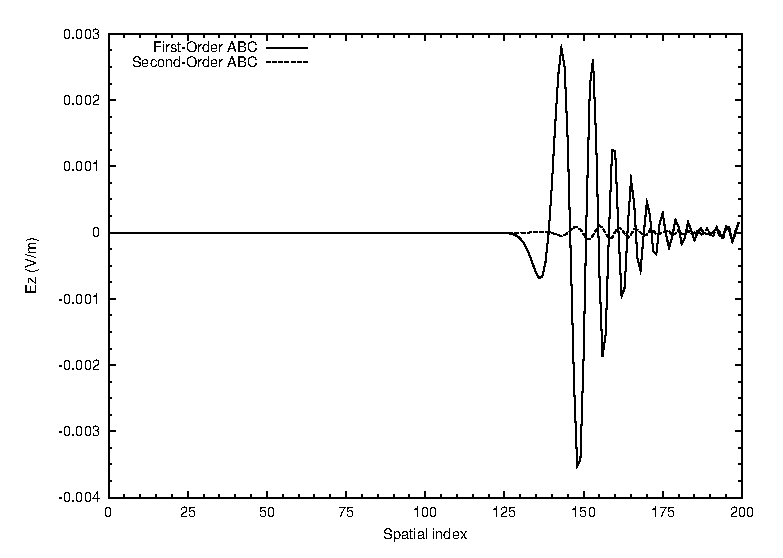
\epsfig{width=4.5in,file=Code/Fdtd-abc/abc-first-second.eps}
  \end{center}
  \caption{Plot of the fields at time step 550 when the grid is
  terminated with either a first- or second-order ABC.  This snapshot
  is taken after the transmitted pulse has encountered the right edge of
  the grid.  Hence this shows the field reflected by the ABC.  Ideally the
  reflected fields should be zero.}
  \label{fig:firstSecondABC}
\end{figure}

\newpage

\section{Implementation of a Second-Order ABC
  \label{sec:secondAbc}}

In order to implement a second-order ABC, one merely has to modify the
functions {\tt abcInit()} and {\tt abc()}.  Thus, none of the code
depicted in Fig.\ \ref{fig:firstOrderAbcFiles} needs to change except
for that which is directly related to the ABC itself.  If instead of
using the file {\tt abcfirst.c}, one uses the code shown in Program
\ref{pro:abcsecond}, which we assume is stored in a file called {\tt
abcsecond.c}, then a second-order ABC will be realized.

\begin{program}
{\tt abcsecond.c} The {\tt abcInit()} and {\tt abc()} functions for
implementation of a second-orde ABC.
\label{pro:abcsecond}
\codemiddle
\begin{lstlisting}
/* Functions to implement a second-order ABC. */

#include "fdtd3.h"
#include <math.h>

static int initDone = 0;
static double *ezOldLeft1, *ezOldLeft2, /*@ \label{abcsecondA} @*/
              *ezOldRight1, *ezOldRight2;
static double *abcCoefLeft, *abcCoefRight; /*@ \label{abcsecondB} @*/

/* Initizalization function for second-order ABC. */
void abcInit(Grid *g) {
  double temp1, temp2;
  
  initDone = 1;

  ALLOC_1D(ezOldLeft1, 3, double); /*@ \label{abcsecondC} @*/
  ALLOC_1D(ezOldLeft2, 3, double);
  ALLOC_1D(ezOldRight1, 3, double);
  ALLOC_1D(ezOldRight2, 3, double);

  ALLOC_1D(abcCoefLeft, 3, double);
  ALLOC_1D(abcCoefRight, 3, double); /*@ \label{abcsecondD} @*/

  /* calculate coefficients on left end of grid */
  temp1 = sqrt(Cezh(0) * Chye(0));
  temp2 = 1.0 / temp1 + 2.0 + temp1;
  abcCoefLeft[0] = -(1.0 / temp1 - 2.0 + temp1) / temp2;
  abcCoefLeft[1] = -2.0 * (temp1 - 1.0 / temp1) / temp2;
  abcCoefLeft[2] = 4.0 * (temp1 + 1.0 / temp1) / temp2;

  /* calculate coefficients on right end of grid */
  temp1 = sqrt(Cezh(SizeX - 1) * Chye(SizeX - 2));
  temp2 = 1.0 / temp1 + 2.0 + temp1;
  abcCoefRight[0] = -(1.0 / temp1 - 2.0 + temp1) / temp2;
  abcCoefRight[1] = -2.0 * (temp1 - 1.0 / temp1) / temp2;
  abcCoefRight[2] = 4.0 * (temp1 + 1.0 / temp1) / temp2;

  return;
}

/* Second-order ABC. */
void abc(Grid *g) {
  int mm;

  /* check if abcInit() has been called */
  if (!initDone) {
    fprintf(stderr,
	    "abc: abcInit must be called before abc.\n");
    exit(-1);
  }

  /* ABC for left side of grid */
  Ez(0) = abcCoefLeft[0] * (Ez(2) + ezOldLeft2[0]) /*@ \label{abcsecondE} @*/
    + abcCoefLeft[1] * (ezOldLeft1[0] + ezOldLeft1[2] -
		        Ez(1) - ezOldLeft2[1])
    + abcCoefLeft[2] * ezOldLeft1[1] - ezOldLeft2[2];

  /* ABC for right side of grid */
  Ez(SizeX-1) =  /*@ \label{abcsecondF} @*/
    abcCoefRight[0] * (Ez(SizeX - 3) + ezOldRight2[0])
    + abcCoefRight[1] * (ezOldRight1[0] + ezOldRight1[2] -
		         Ez(SizeX - 2) - ezOldRight2[1])
    + abcCoefRight[2] * ezOldRight1[1] - ezOldRight2[2];

  /* update stored fields */
  for (mm = 0; mm < 3; mm++) {  /*@ \label{abcsecondG} @*/
    ezOldLeft2[mm] = ezOldLeft1[mm];
    ezOldLeft1[mm] = Ez(mm);
    
    ezOldRight2[mm] = ezOldRight1[mm];
    ezOldRight1[mm] = Ez(SizeX - 1 - mm);
  }

  return;
}
\end{lstlisting}
\end{program}

Lines \ref{abcsecondA}--\ref{abcsecondB} declare six static, global
pointers, each of which will ultimately serve as an array of three
points.  Four of the arrays will store previous values of the electric
field (two arrays dedicated to the left side and two to the right).
The remaining two arrays store the coefficients used in the ABC (one
array for the left, one for the right).  The memory for these arrays
is allocated in the {\tt abcInit()} function in lines
\ref{abcsecondC}--\ref{abcsecondD}.  That is followed by calculation
of the coefficients on the two side of the grid.

Within the function {\tt abc()}, which is called once per time-step,
the values of the nodes on the edge of the grid are updated by the
statements starting on lines
\ref{abcsecondE} and \ref{abcsecondF}.  Finally, starting on line
\ref{abcsecondG}, the stored values are updated.  The array {\tt
exOldLeft1} represents the field one time-step in the past while 
{\tt exOldLeft2} represents the field two time-steps in the past.
Similar naming is employed on the right.

\chapter{Dispersion, Impedance, Reflection, and Transmission
 \label{chap:dispersion}}

%\setcounter{page}{1}

\renewcommand{\thefootnote}{\fnsymbol{footnote}}
\footnotetext[2]{Lecture notes by John Schneider.  {\tt
fdtd-dispersion.tex}}

\section{Introduction}

A dispersion relation gives the relationship between frequency and
the speed of propagation.  This relationship is rather simple in the
continuous world and is reviewed in the next section.  Unfortunately
dispersion in the FDTD is not as simple.  Nevertheless, it provides a
great deal of insight into the inherent limitations of the FDTD method
and hence it is important that one have at least a basic understanding
of it.

The tools developed in the analysis of FDTD dispersion can also be
used to determine the characteristic impedance of the grid.
Furthermore, as will be shown, knowing the dispersion relationship
one can obtain exact analytic expressions for the reflection and
transmission coefficients in the FDTD grid.

\section{Dispersion in the Continuous World}

Consider a plane wave propagating in the $+x$ direction in a
lossless medium.  In time-harmonic form the temporal and spatial
dependence of the wave are given by $\exp(j[\omega t-\beta x])$ where
$\omega$ is the frequency and $\beta$ is the phase constant (wave number).
The speed of the wave can be found by determining how fast a given
point on the wave travels.  In this context ``point'' is taken to mean
a point of constant phase.  The phase is dictated by $\omega t - \beta x$.
Setting this equal to a constant and differentiating with respect to
time gives
\begin{eqnarray}
  \frac{d}{dt}(\omega t-\beta x) &=& \frac{d}{dt}(\mbox{constant}), \\
  \omega - \beta \frac{dx}{dt} &=& 0. \label{eq:phase}
\end{eqnarray}
In this expression $x$ is taken to be the position which provides a
particular phase.  In that sense it is not an independent variable.
The location $x$ which yields the desired phase will change as a
function of time.  Therefore, $dx/dt$ is the speed of the wave, or,
more properly, the phase speed $c_p$.  Solving \refeq{eq:phase} for the
phase speed yields
\begin{equation}
  c_p = \frac{dx}{dt} = \frac{\omega}{\beta}.
\end{equation}
This is apparently a function of frequency, but for a plane wave the
phase constant $\beta$ is given by $\omega\sqrt{\mu\epsilon}$.  Thus
the phase speed is
\begin{equation}
  c_p = \frac{\omega}{\omega\sqrt{\mu\epsilon}} 
  = \frac{1}{\sqrt{\mu_r\mu_0\epsilon_r\epsilon_0}} 
  = \frac{c}{\sqrt{\mu_r\epsilon_r}}
\end{equation}
where $c$ is the speed of light in free space.  Note that, in the
continuous world for a lossless medium, the phase speed is independent
of frequency and the dispersion relationship is
\begin{equation}
 c_p = \frac{\omega}{\beta} = \frac{c}{\sqrt{\mu_r\epsilon_r}}.
 \label{eq:dispExact1D} 
\end{equation}
Since $c$ is a constant, and we are assuming $\mu_r$ and $\epsilon_r$
contact for the given material, all frequencies propagate at the same
speed.  Unfortunately this is not the case in the discretized FDTD
world---different frequencies have different phase
speeds.\footnote{Later we will consider FDTD models of materials that
  are dispersive in the continuous world, i.e., materials for which
  $\epsilon$ or $\mu$ are functions of frequency.  In fact, we have
  already considered dispersive behavior to some degree since lossy
  materials have phase speeds that are a function of frequency.}

\section{Harmonic Representation of the FDTD Method}

The spatial shift-operator $s_x$ and the temporal shift-operator
$s_t$ were introduced in Sec.\ \ref{sec:abcOperator}.  Generalizing
these slightly, let a fractional superscript represent a corresponding
fractional step.  For example,
\begin{eqnarray}
  s_x^{1/2}\fdtd{H_y}{m}{q} &=& \fdtdh{H_y}{m+\half}{q}, \\
  s_t^{1/2}\fdtd{E_z}{m}{q+\half} &=& \fdtd{E_z}{m}{q+1}, \\
  s_t^{-1/2}\fdtd{E_z}{m}{q+\half} &=& \fdtd{E_z}{m}{q}.
\end{eqnarray}
Using these shift operators the finite-difference version of Ampere's
law (ref.\ \refeq{eq:ampereFdtd1D}) can be written
\begin{equation}
  \epsilon
  \left(\frac{s_t^{1/2} - s_t^{-1/2}}{\Delt}\right)\fdtd{E_z}{m}{q+\half}
  =
  \left(\frac{s_x^{1/2} - s_x^{-1/2}}{\Delx}\right)\fdtdh{H_y}{m}{q+\half}.
  \label{eq:ampereShift}
\end{equation}
Note that both fields have a temporal index of $q+1/2$.  The index can
be changed to $q$ if the $1/2$ is accounted for by a temporal shift.
Thus Ampere's law can also be written
\begin{equation}
  s_t^{1/2}\epsilon
  \left(\frac{s_t^{1/2} - s_t^{-1/2}}{\Delt}\right)\fdtd{E_z}{m}{q}
  =
  s_t^{1/2}
  \left(\frac{s_x^{1/2} - s_x^{-1/2}}{\Delx}\right)\fdtd{H_y}{m}{q}.
  \label{eq:ampereShiftI}
\end{equation}

Let us define the finite-difference operator $\tpartial_i$ as
\begin{equation}
  \tpartial_i = \left(\frac{s_i^{1/2} - s_i^{-1/2}}{\Delta_i}\right)
\end{equation}
where $i$ is either $x$ or $t$.  Using this notation the Yee version
of Ampere's law can be written
\begin{equation}
  \epsilon s_t^{1/2}
  \tpartial_t\fdtd{E_z}{m}{q}
  =
  s_t^{1/2}
  \tpartial_x\fdtd{H_y}{m}{q}.
  \label{eq:ampereShiftII}
\end{equation}

Rather than obtaining an update equation from this, the goal is to
determine the phase speed for a given frequency.  To that end, we
assume there is a single harmonic wave propagating such that
\begin{eqnarray}
  \fdtd{\hat{E}_z}{m}{q} &=& \hat{E}_0 e^{j(\omega q \Delt - \tbeta m \Delx)}, 
  \label{eq:ezEigen} \\
  \fdtd{\hat{H}_y}{m}{q} &=& \hat{H}_0 e^{j(\omega q \Delt - \tbeta m \Delx)},
  \label{eq:hyEigen}
\end{eqnarray}
where $\tbeta$ is the phase constant which exists in the FDTD grid and
$\hat{E}_0$ and $\hat{H}_0$ are constant amplitudes.  A tilde will be
used to indicate quantities in the FDTD grid which will typically (but
not always!)  differ from the corresponding value in the continuous
world.  Thus, the phase constant $\tbeta$ in the FDTD grid will
differ, in general, from the phase constant $\beta$ in the continuous
world.  As was done in Sec.\ \ref{sec:specExampleTrans} a caret (hat) will
be used to indicate a harmonic quantity.

We will assume the frequency $\omega$ is the same in both the FDTD
grid and the continuous world.  Note that one has complete control
over the frequency of the excitation---one merely has to ensure that
the phase of the source changes a particular number of radians every
time step.  However, one does not have control over the phase
constant, i.e., the spatial frequency.  The grid dictates what
$\tbeta$ will be for a given temporal frequency.

The plane-wave space-time dependence which appears in
\refeq{eq:ezEigen} and \refeq{eq:hyEigen} essentially serves as an
eigenfunction for the FDTD governing equations.  If the governing
equations operate on a function with this dependence, they will yield
another function which has the same space-time dependence, albeit
scaled by some value.  To illustrate this, consider the temporal
shift-operator acting on the electric field
\begin{eqnarray}
  s_t^{\pm 1/2}\fdtd{\hat{E}_z}{m}{q} &=&
    \hat{E}_0 e^{j[\omega (q\pm 1/2) \Delt - \tbeta m \Delx]}
    \nonumber \\
   &=&
     e^{\pm j\omega\Delt/2}
     \hat{E}_0 e^{j[\omega q \Delt - \tbeta m \Delx]}
     \nonumber \\
   &=&
     e^{\pm j\omega\Delt/2}
    \fdtd{\hat{E}_z}{m}{q}.
\end{eqnarray}
Similarly, the spatial shift-operator acting on the electric field
yields
\begin{eqnarray}
  s_x^{\pm 1/2}\fdtd{\hat{E}_z}{m}{q} &=&
    \hat{E}_0 e^{j[\omega q \Delt - \tbeta (m \pm 1/2) \Delx]}
    \nonumber\\
   &=&
    e^{\mp j\tbeta\Delx/2}
    \hat{E}_0 e^{j[\omega q \Delt - \tbeta m \Delx]}
    \nonumber\\
   &=&
    e^{\mp j\tbeta\Delx/2}
    \fdtd{\hat{E}_z}{m}{q}.
\end{eqnarray}
Thus, for a plane wave, one can equate the shift operators with
multiplication by an appropriate term:
\begin{eqnarray}
  s_t^{\pm 1/2} &\Leftrightarrow& e^{\pm j\omega\Delt/2}, 
  \label{eq:temporalShiftEquiv}
  \\
  s_x^{\pm 1/2} &\Leftrightarrow& e^{\mp j\tbeta\Delx/2}.
\end{eqnarray}
Carrying this a step further, for plane-wave propagation the
finite-difference operators $\tpartial_t$ and $\tpartial_x$ are
equivalent to
\begin{eqnarray}
  \tpartial_t &=& \frac{e^{+j\omega\Delt/2}-e^{-j\omega\Delt/2}}{\Delt} 
         \,=\, j\frac{2}{\Delt}\sin\left(\frac{\omega\Delt}{2}\right), \\
  \tpartial_x &=& \frac{e^{-j\tbeta\Delx/2}-e^{+j\tbeta\Delx/2}}{\Delx} 
         \,=\, -j\frac{2}{\Delx}\sin\left(\frac{\tbeta\Delx}{2}\right).
\end{eqnarray}
We define $\Omega$ and $K_x$ as
\begin{eqnarray}
  \Omega &=& \frac{2}{\Delt}\sin\left(\frac{\omega\Delt}{2}\right), \\
  K_x &=& \frac{2}{\Delx}\sin\left(\frac{\tbeta\Delx}{2}\right).
  \label{eq:KxDefinition}
\end{eqnarray}
Note that as the discretization goes to zero, $\Omega$ approaches
$\omega$ and $K_x$ approaches $\tbeta$ (and, in fact, $\tbeta$ would
approach $\beta$, the phase constant in the continuous world).  Using this
notation, taking a finite-difference with respect to time is
equivalent to multiplication by $j\Omega$ while a finite difference
with respect to space is equivalent to multiplication by $-jK_x$,
i.e.,
\begin{eqnarray}
  \tpartial_t &\Leftrightarrow& j\Omega \label{eq:OmegaDef} \\
  \tpartial_x &\Leftrightarrow& -jK_x.  \label{eq:KDef}
\end{eqnarray}

Using \refeq{eq:temporalShiftEquiv}, \refeq{eq:OmegaDef}, and
\refeq{eq:KDef} in Ampere's law \refeq{eq:ampereShiftII} yields
\begin{equation}
  j \epsilon \Omega e^{j\omega\Delt/2} 
    \fdtd{\hat{E}_z}{m}{q}
  =
   -j K_x e^{j\omega\Delt/2} 
    \fdtd{\hat{H}_y}{m}{q}.
  \label{eq:ampereOperator}
\end{equation}
The temporal shift $\exp(j\omega\Delt/2)$ is common to both side and
hence can be canceled.  Using the assumed form of the electric and
magnetic fields from \refeq{eq:ezEigen} and \refeq{eq:hyEigen} in
\refeq{eq:ampereOperator} yields
\begin{equation}
  \epsilon \Omega \hat{E}_0 e^{j(\omega q \Delt - \tbeta m \Delx)} =
   - K_x \hat{H}_0 e^{j(\omega q \Delt - \tbeta m \Delx)}.
\end{equation}
Canceling the exponential space-time dependence which is common to
both sides produces
\begin{equation}
  \epsilon \Omega \hat{E}_0 = - K_x \hat{H}_0.
\end{equation}
Solving for the ratio of the electric and magnetic field amplitudes
yields
\begin{equation}
  \frac{\hat{E}_0}{\hat{H}_0} = -\frac{K_x}{\epsilon\Omega} = 
  - \frac{\Delt}{\epsilon\Delx}
    \frac{\sin\!\left(\frac{\tbeta\Delx}{2}\right)}
       {\sin\!\left(\frac{\omega\Delt}{2}\right)}.
  \label{eq:dispAmperePart}
\end{equation}

It appears that \refeq{eq:dispAmperePart} is the ``numeric impedance''
since it is the ratio of the electric field to the magnetic field.  In
fact it {\em is} the numeric impedance, but it is only part of the
story.  As will be shown, the impedance in the FDTD method is exact.
This fact is far from obvious if one only considers
\refeq{eq:dispAmperePart}.  It is also worth considering the
corresponding continuous-world quantity $\beta/(\epsilon\omega)$:
\begin{equation}
  \frac{\beta}{\epsilon\omega} = \frac{\omega/c_p}{\epsilon\omega}
  = \frac{1}{\epsilon c_p} =  \frac{\sqrt{\mu\epsilon}}{\epsilon}
  = \sqrt{\frac{\mu}{\epsilon}} = \eta
\end{equation}
Thus the fact that the grid numeric impedance is given by
$K_x/(\epsilon\Omega)$ is consistent with continuous-world behavior.
(The negative sign in \refeq{eq:dispAmperePart} merely accounts for
the orientation of the fields.)

\section{Dispersion in the FDTD Grid \label{sec:gridDispersion}}

Another equation relating $\hat{E}_0$ and $\hat{H}_0$ can be obtained
from Faraday's law.  Expressed in terms of shift operators, the
finite-difference form of Faraday's law
(ref.\ \refeq{eq:faradayFdtd1D}) is
\begin{equation}
  \mu s_x^{1/2}\tpartial_t\fdtd{\hat{H}_y}{m}{q} =
  s_x^{1/2}\tpartial_x\fdtd{\hat{E}_z}{m}{q}.  
  \label{eq:faradayShift}
\end{equation}
As before, assuming plane-wave propagation, the shift operators can be
replaced with multiplicative equivalents.  The resulting equation is
\begin{equation}
  j\mu \Omega e^{-j\omega\Delx/2}
   \fdtd{\hat{H}_y}{m}{q}
  =
   -j K_x e^{-j\omega\Delx/2}
   \fdtd{\hat{E}_z}{m}{q}.
\end{equation}
Canceling terms common to both sides and rearranging yields
\begin{equation}
  \frac{\hat{E}_0}{\hat{H}_0} = 
  -\frac{\mu\Omega}{K_x}
  =
  -\frac{\mu\Delx}{\Delt}
  \frac{\sin\!\left(\frac{\omega\Delt}{2}\right)}
       {\sin\!\left(\frac{\tbeta\Delx}{2}\right)}.
  \label{eq:dispFaradayPart}
\end{equation}
Equating \refeq{eq:dispAmperePart} and \refeq{eq:dispFaradayPart} and
cross-multiplying gives
\begin{equation}
  \mu\epsilon\Omega^2 = K_x^2.
  \label{eq:fdtdDispersionOneD}
\end{equation}
This is the FDTD dispersion relation.  Alternatively, expanding terms
and rearranging slightly yields
\begin{equation}
  \sin^2\left(\frac{\omega\Delt}{2}\right) =
  \frac{\Delt^2}{\epsilon\mu\Delx^2}
  \sin^2\left(\frac{\tbeta\Delx}{2}\right).
\end{equation}
Taking the square root of both sides of either form of the dispersion
relation yields
\begin{equation}
  \sqrt{\mu\epsilon}\Omega = K_x,
  \label{eq:disp1DOmegaK}
\end{equation}
or
\begin{equation}
  \sin\!\left(\frac{\omega\Delt}{2}\right) =
  \frac{\Delt}{\sqrt{\epsilon\mu}\Delx}
  \sin\!\left(\frac{\tbeta\Delx}{2}\right).
  \label{eq:disp1D}
\end{equation}
These equations dictate the relationship between $\omega$ and
$\tbeta$.  Contrast this to the dispersion relation
\refeq{eq:dispExact1D} which pertains to the continuous world.  The
two appear quite dissimilar!  However, the two equations do agree in
the limit as the discretization gets small.

The first term in the Taylor series expansion of $\sin(\xi)$ is $\xi$.
Thus $\xi$ provides a good approximation of $\sin(\xi)$ when $\xi$ is
small.  Assume that the spatial and temporal steps are small enough so
that the arguments of the sine functions in \refeq{eq:disp1D} are
small.  Retaining the first-order term in the Taylor-series expansion
of the sine functions in \refeq{eq:disp1D} yields
\begin{equation}
  \frac{\omega\Delt}{2} =
  \frac{\Delt}{\sqrt{\epsilon\mu}\Delx}
  \frac{\tbeta\Delx}{2}.
\end{equation}
From this $\tbeta$ is seen to be
\begin{equation}
 \tbeta = \omega\sqrt{\mu\epsilon},
\end{equation}
which is exactly the same as in the continuous world.  However, this
is only true when the discretization goes to zero.  For finite
discretization, the phase speed in the FDTD grid and in the continuous
world differ.

In the continuous world the phase speed is $c_p=\omega/\beta$.  In the
FDTD world the same relation holds, i.e., $\tilde{c}_p=\omega/\tbeta$
where the tilde indicates this is the phase speed in the discretized
world.  In one dimension, a closed form solution for $\tbeta$ is possible
(a similar dispersion relation holds in two and three dimensions, but
there a closed-form solution is not possible).  Bringing the
coefficient to the other side of \refeq{eq:disp1D} and taking the
arc sine yields
\begin{equation}
  \frac{\tbeta\Delx}{2} = \sin^{-1}\!\left[
     \frac{\Delx\sqrt{\mu\epsilon}}{\Delt}
     \sin\!\left(\frac{\omega\Delt}{2}\right)\right].
  \label{eq:tbeta}
\end{equation}
As was shown in Sec.\ \ref{sec:harmonicSources} (ref.\
\refeq{eq:fHarmonic} and \refeq{eq:fHarmonicI}), the factor
$\omega\Delt/2$ is equivalent to $\pi S_c/\ppw$ where
$S_c=c\Delt/\Delx$.  Thus \refeq{eq:tbeta} can be written
\begin{equation}
  \frac{\tbeta\Delx}{2} = \sin^{-1}\left[
    \frac{\sqrt{\mu_r\epsilon_r}}{S_c}
    \sin\!\left(\frac{\pi S_c}{\ppw}\right)\right].
  \label{eq:tbetaI}
\end{equation}

Consider the ratio of the phase speed in the grid to the true phase
speed
\begin{equation}
  \frac{\tilde{c}_p}{c_p} = 
  \frac{\omega/\tbeta}{\omega/\beta} = \frac{\beta}{\tbeta}
  = \frac{\frac{\beta\Delx}{2}}{\frac{\tbeta\Delx}{2}}.
  \label{eq:phaseRatio}
\end{equation}
The phase constant in the continuous world can be written
\begin{equation}
  \beta=\omega\sqrt{\mu\epsilon}
  = 2 \pi \frac{c}{\lambda}\sqrt{\mu_0\epsilon_0\mu_r\epsilon_r}
  = \frac{2 \pi}{\lambda}\sqrt{\mu_r\epsilon_r}
  = \frac{2 \pi}{\ppw \Delx}\sqrt{\mu_r\epsilon_r}
\end{equation}
where $\ppw$ is the number of points per free-space wavelength.  Using
this in the numerator of the last term on the right-hand side of
\refeq{eq:phaseRatio} and using \refeq{eq:tbetaI} in the denominator,
this ratio becomes
\begin{equation}
  \frac{\tilde{c}_p}{c_p} = \frac{\pi\sqrt{\mu_r\epsilon_r}}{\ppw
  \sin^{-1}\left[\frac{\sqrt{\mu_r\epsilon_r}}{S_c}
  \sin\!\left(\frac{\pi S_c}{\ppw}\right)\right]}.
\end{equation}
This equation is a function of the material parameters ($\epsilon_r$
and $\mu_r$), the Courant number ($S_c$), and the number of points per
wavelength ($\ppw$).

For propagation in free space, i.e., $\epsilon_r=\mu_r=1$, when there
are $20$ points per wavelength and the Courant number $S_c$ is $1/2$,
the ratio of the numeric to the exact phase speed is approximately
$0.9969$ representing an error of $0.31$ percent.  Thus, for every
wavelength of travel, the FDTD wave will accumulate about $1.12$
degrees of phase error ($0.0031\times 360$).  If the discretization is
lowered to $10$ points per wavelength, the ratio drops to $0.9873$, or
about a $1.27$ percent error.  Note that as the discretization was
halved, the error increased by roughly a factor of four.  This is as
should be expected for a second-order method.

Consider the case of propagation in free space and a Courant number of
$1$.  In that case the ratio collapses to
\begin{equation}
  \frac{\tilde{c}_p}{c_p} = 
  \frac{\pi}{\ppw
    \sin^{-1}\left[
    \sin\!\left(\frac{\pi}{\ppw}\right)\right]} = 1.
\end{equation}
Thus the phase speed in the FDTD grid is exactly what it is in the
continuous world!  This is true for all discretization.

Figure \ref{fig:dispError} shows a plot of the ratio of the FDTD and
exact phase speeds as a function of discretization.  Three different
Courant numbers are used.  Ideally the ratio would be unity for all
discretizations.  As can be seen, the greater the Courant number, the
closer the curve is to ideal.  A large Courant number is thus
desirable for two reasons.  First, the larger the Courant number, the
greater the temporal step and hence the more quickly a simulation
advances (i.e., each update represents a greater advance in time).
Second, the larger the Courant number, the smaller the dispersion
error.  In one dimension a Courant number of unity is the greatest
possible and, since there is no dispersion error with this Courant
number, the corresponding time step is known as the magic time-step.
Unfortunately a magic time-step does not exist in higher dimensions.

\begin{figure}
  \begin{center}
  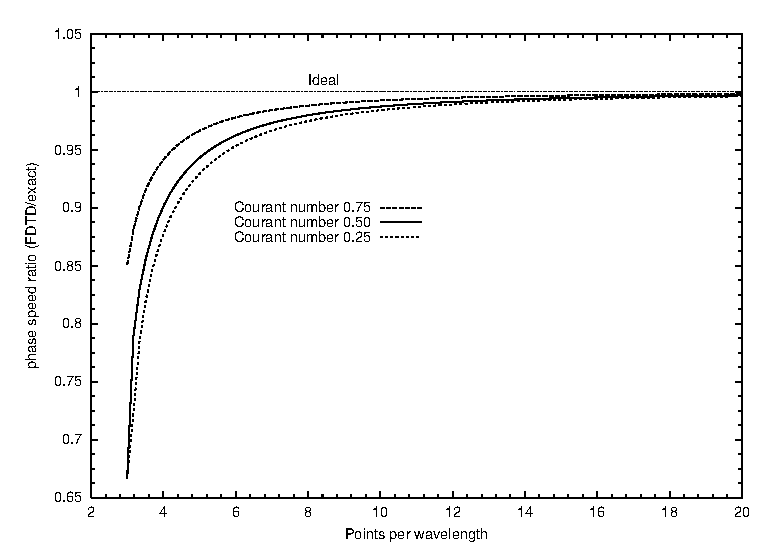
\epsfig{width=5.in,file=Code/Fdtd-dispersion/disp-error.eps}
  \end{center}
  \caption{Ratio of the FDTD and exact phase speeds
  ($\tilde{c}_p/c_p$) versus the discretization.  Propagation in free
  space is assumed.  Ideally the ratio would be unity for all
  discretizations.  Courant numbers of $1/4$, $1/2$, and $3/4$ are
  considered.}  \label{fig:dispError}
\end{figure}

Figure \ref{fig:dispDemo} shows snapshots of Ricker wavelets
propagating to the right that have been discretized at either $20$ or
$10$ points per wavelength at the most energetic frequency (i.e., the
parameter $N_P$ discussed in Sec.\ \ref{sec:ricker} is either $20$ or $10$).
The wavelets are propagating in grids that have a Courant number of
either $1$ or $0.5$.  In Figs.\ \ref{fig:dispDemo}(a) and (b) the
discretizations are $20$ and $10$, respectively, and the Courant
number is unity.  Since this corresponds to the magic time-step, the
wavelets propagate without distortion.  The discretizations in
Figs.\ \ref{fig:dispDemo}(c) and (d) are also $20$ and $10$,
respectively, but now the Courant number is $0.5$.  The snapshots in
(a) and (b) were taken after $100$ time-steps while the snapshots in
(c) and (d) were taken after $200$ time-steps (since the time step is
half as large in (c) and (d) as it is in (a) and (b), this ensures the
snapshots are depicting the field at the same time).  In
Fig.\ \ref{fig:dispDemo}(c) the distortion of the Ricker wavelet is
visible in that the function is no longer symmetric about the peak.
In Fig.\ \ref{fig:dispDemo}(d) the distortion caused by dispersion is
rather extreme and the function is no longer recognizable as a Ricker
wavelet.  The reason that Fig.\ \ref{fig:dispDemo}(d) is so much more
distorted than Fig.\ \ref{fig:dispDemo}(c) is that the spectral energy
lies at a coarser discretization.  The more coarsely a harmonic is
discretized, the more dispersion it will suffer---the higher
frequencies propagate more slowly than the lower frequencies.  This
causes the ringing that is evident on the trailing side of the pulse.

\begin{figure}
  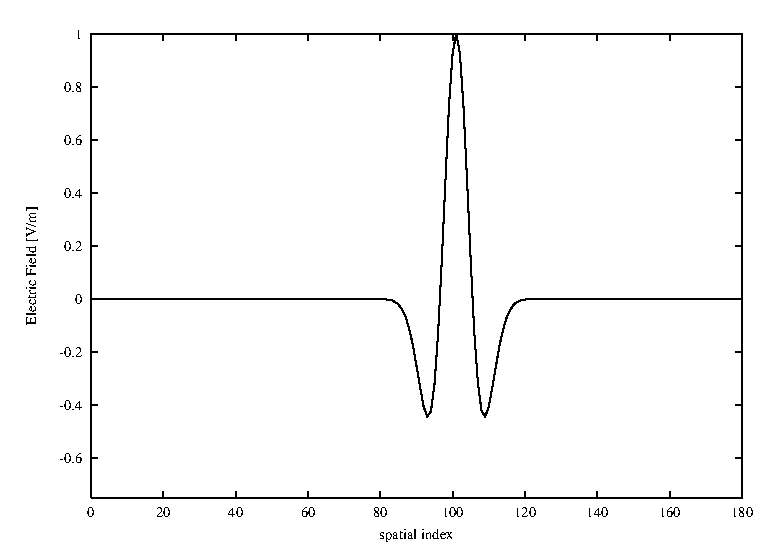
\epsfig{width=3.2in,file=Code/Fdtd-dispersion/disp-s1-ppw20.eps}
  \hspace{.1in}
  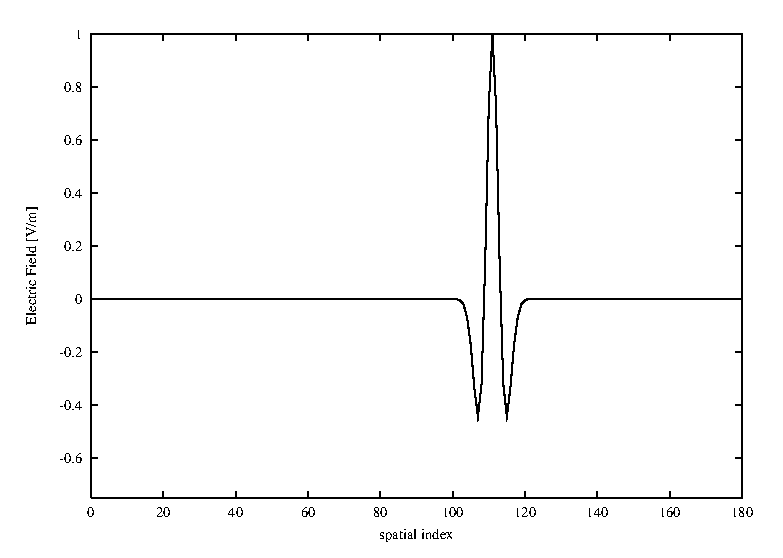
\epsfig{width=3.2in,file=Code/Fdtd-dispersion/disp-s1-ppw10.eps}\\
  \mbox{}\hspace{1.in}(a) $N_P=20$, $S_c=1$
         \hspace{1.95in}(b) $N_P=10$, $S_c=1$\\

  \vspace{.1in}
  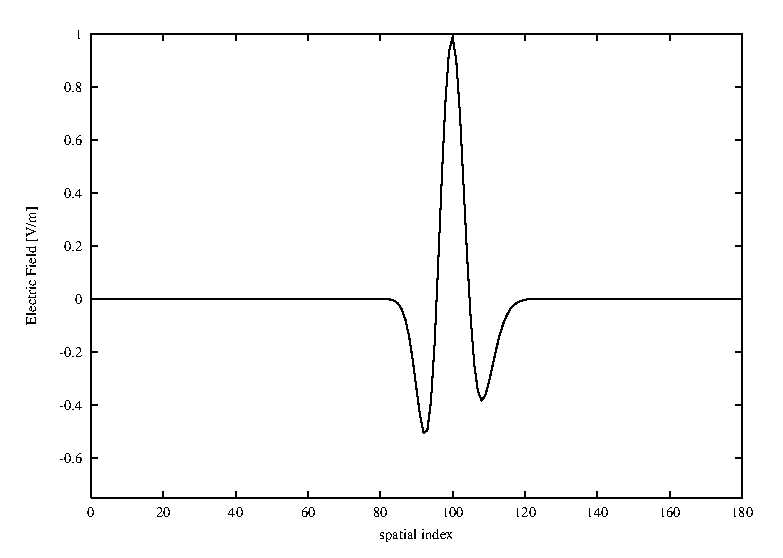
\epsfig{width=3.2in,file=Code/Fdtd-dispersion/disp-s0p5-ppw20.eps}
  \hspace{.1in}
  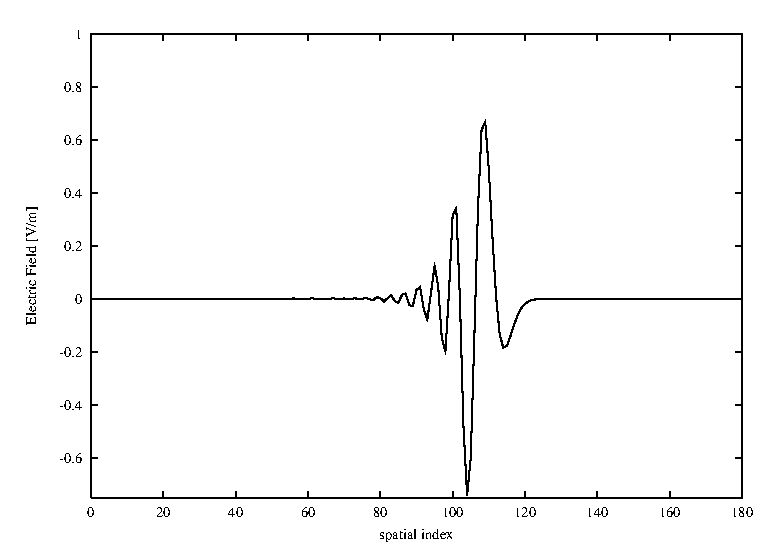
\epsfig{width=3.2in,file=Code/Fdtd-dispersion/disp-s0p5-ppw10.eps}\\
  \mbox{}\hspace{.95in}(c) $N_P=20$, $S_c=0.5$
         \hspace{1.95in}(d) $N_P=10$, $S_c=0.5$
  \caption{Snapshots of Ricker wavelets with different discretization
  propagating in grids with different Courant numbers.  (a) $20$
  points per wavelength at the most energetic frequency, i.e.,
  $N_P=20$, $S_c=1$, (b) $N_P=10$, $S_c=1$, (c) $N_P=20$, $S_c=0.5$,
  and (d) $N_P=10$, $S_c=0.5$.  The snapshots were taken after $100$
  time-steps for (a) and (b), and after $200$ time-steps for (c) and
  (d).}  \label{fig:dispDemo}
\end{figure}



\section{Numeric Impedance}

Let us return to \refeq{eq:dispAmperePart} which nominally gave the numeric
impedance and which is repeated below
\begin{equation}
  \frac{\hat{E}_0}{\hat{H}_0} = -\frac{K_x}{\epsilon\Omega}.
  \label{eq:impedance}
\end{equation}
The dispersion relation \refeq{eq:disp1DOmegaK} expressed $K_x$ in
terms of $\Omega$.  Plugging this into \refeq{eq:impedance} yields
\begin{equation}
  \frac{\hat{E}_0}{\hat{H}_0} =
     -\frac{\sqrt{\mu\epsilon}\Omega}{\epsilon\Omega} = 
     \sqrt{\frac{\mu}{\epsilon}} =
     \eta.
  \label{eq:impedanceI}
\end{equation}
Thus, despite the inherent approximations in the FDTD method, the
impedance in the grid is exactly the same as in the continuous world
(this also holds in higher dimensions).

\section{Analytic FDTD Reflection and Transmission
  Coefficients}

Section \ref{sec:measureTrans} discussed the way in which an FDTD
simulation could be used to measure the transmission coefficient
associated with a planar interface.  In this section, instead of using
a simulation to measure the transmission coefficient, an expression
will be derived that gives the transmission coefficient for the FDTD
grid.

Consider a one-dimensional FDTD simulation as shown in
Fig.\ \ref{fig:oneDHalfSpace}.  The permittivity changes abruptly at
the magnetic field which is assumed to coincide with the interface at
$x=0$.  The permeability is constant throughout the computational
domain.  

\begin{figure}
  \begin{center}
  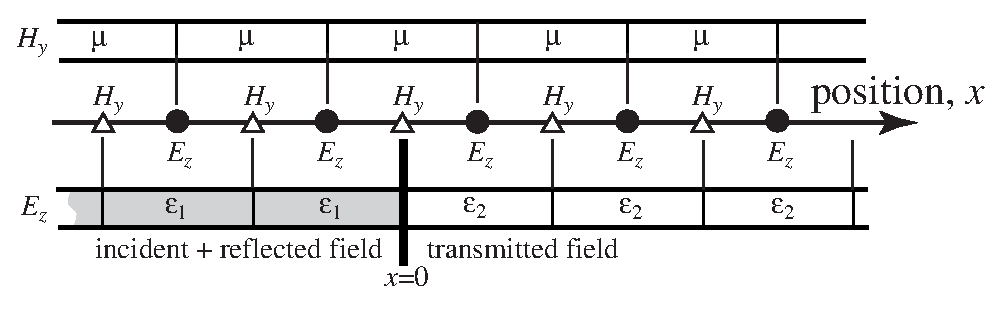
\epsfig{width=5.in,file=Figures/Fdtd-dispersion/dielectric-discontinuity.eps}
  \end{center} \caption{One-dimensional simulation where the
  permittivity changes abruptly at $x=0$.  The interface between the
  two media coincides with a magnetic-field node.  The permeability is
  assumed to be constant throughout the computational domain.  The
  figure depicts the nodes and the material values associated with
  their updates.  The field to the left of the interface is the sum of
  the incident and reflected fields.  The transmitted field exists to
  the right of the boundary.}  \label{fig:oneDHalfSpace}
\end{figure}

Assume there is an incident unit-amplitude plane wave propagating in
the $+x$ direction.  Because of the change in permittivity, a
reflected field will exist to the left of the boundary which
propagates in the $-x$ direction.  Additionally, there will be a
transmitted field which propagates to the right of the boundary.  The
incident, reflected, and transmitted electrics fields are given by
\begin{eqnarray}
   \Eifdtdq &=& \Eifdtd e^{j\omega q\Delt} =
                e^{-j\tbeta_1 m\Delx}e^{j\omega q\Delt},
     \label{eq:eInc} \\
   \Erfdtdq &=& \Erfdtd e^{j\omega q\Delt} =
                \Gfdtd e^{j\tbeta_1 m\Delx}e^{j\omega q\Delt}, \\
   \Etfdtdq &=& \Etfdtd e^{j\omega q\Delt} =
                \Tfdtd e^{-j\tbeta_2 m\Delx}e^{j\omega q\Delt}
     \label{eq:eTrans}
\end{eqnarray}
where $\Gfdtd$ and $\Tfdtd$ are the FDTD reflection and transmission
coefficients, respectively.  Note that all fields will have the
common temporal phase factor $\exp(j\omega q\Delt)$.  Therefore this
term will not be explicitly written (its existence is implicit in the
fact that we are doing harmonic analysis).

As shown in the previous section, the characteristic impedance in the
FDTD grid is exact.  Therefore the magnetic fields can be related to
the electric fields in the same manner as they are in the continuous
world, i.e.,
\begin{eqnarray}
   \Hifdtd &=& -\frac{1}{\eta_1}e^{-j\tbeta_1 m\Delx},
     \label{eq:hInc}\\
   \Hrfdtd &=& \frac{\Gfdtd }{\eta_1}e^{j\tbeta_1 m\Delx}, \\
   \Htfdtd &=& -\frac{\Tfdtd}{\eta_2} e^{-j\tbeta_2 m\Delx}.
     \label{eq:hTrans}
\end{eqnarray}

The incident and reflected waves exist to the left of the interface
and the transmitted field exists to the right of the interface.  The
magnetic field at the interface, i.e., the node at $x=0$ is, in a
sense, common to both the left and the right half-spaces.  The field
at this node can be described equally well as the sum of the
incident and reflected waves or by the transmitted wave.  This node
enforces the continuity of the magnetic field across the boundary.
Hence, just as in the continuous world, the fields are governed by the
equation
\begin{equation}
  -\frac{1}{\eta_1} + \frac{\Gfdtd}{\eta_1} = -\frac{\Tfdtd}{\eta_2}.
  \label{eq:magContinuity}
\end{equation}

In the continuous world enforcing the continuity of the tangential
electric and magnetic fields at a boundary yields two equations.
These two equations can be used to solve for the reflection and
transmission coefficients as was shown in Sec.\ \ref{sec:contTrans}.
In FDTD, however, there are no electric field nodes that coincide with
the interface (at least not with this geometry).  Therefore continuity
of the electric fields cannot be enforced directly nor is there a
readily available second equation with which to solve for the
reflection and transmission coefficients.

The necessary second equation is obtained by considering the update
equation for the magnetic field at the interface.  This node depends
on the electric field to either side of the interface and hence ties
the two half-spaces together.  Specifically, the harmonic form of
Faraday's law which governs the magnetic-field node at the interface
can be used to write the following
\begin{eqnarray}
  \left.\mu s_x^{1/2}\tpartial_t\fdtd{\hat{H}_y}{m}{q}\right|_{x=0} &=&
  \left.s_x^{1/2}\tpartial_x\fdtd{\hat{E}_z}{m}{}\right|_{x=0},
  \\
  \left.\mu j\Omega\fdtd{\hat{H}_y}{m}{}\right|_{x=0} &=&
  \left.\frac{1}{\Delx}\left(s_x^{1/2} - s_x^{-1/2}\right)
     \fdtd{\hat{E}_z}{m}{q}\right|_{x=0},
  \\
  \left.j\Omega \fdtd{\hat{H}_y}{m}{}\right|_{x=0} &=&
  \frac{1}{\mu\Delx}
     \left(\Tfdtd e^{-j\tbeta_2\Delx/2} - 
           \left[e^{j\tbeta_1\Delx/2} + \Gfdtd e^{-j\tbeta_1\Delx/2}\right]\right).
  \label{eq:interfaceEqII}
\end{eqnarray}
In the last form of the equation, we have used the fact that the
transmitted field is present when space is shifted a half spatial-step
in the $+x$ direction relative to the boundary.  Conversely the field
is the sum of the incident and reflected waves when space is shifted a
half spatial-step in the $-x$ direction relative to the boundary.

Equation \refeq{eq:interfaceEqII} provides the second equation which,
when coupled to \refeq{eq:magContinuity}, can be used to solve for the
transmission and reflection coefficients.  However, what is
$\left.\fdtd{\hat{H}_y}{m}{}\right|_{x=0}$?  Since this node is on the
interface, the expression for either the transmitted field or the sum
of the incident and reflected field can be used.  Using the
transmitted field (evaluated at $m=0$), the equation becomes
\begin{equation}
  j\Omega \left(-\frac{\Tfdtd}{\eta_2}\right) =
  \frac{1}{\mu\Delx}
     \left(\Tfdtd e^{-j\tbeta_2\Delx/2} - 
           \left[e^{j\tbeta_1\Delx/2} + \Gfdtd e^{-j\tbeta_1\Delx/2}\right]\right).
  \label{eq:usedTrans}
\end{equation}
Regrouping terms yields
\begin{equation}
  e^{j\tbeta_1\Delx/2} + \Gfdtd e^{-j\tbeta_1\Delx/2} =
  \left(e^{-j\tbeta_2\Delx/2} + j\frac{\Omega\mu\Delx}{\eta_2}\right) \Tfdtd.
  \label{eq:magContinuityI}
\end{equation}
After multiplying through by $-\eta_1\exp(-j\tbeta_1\Delx/2)$,
\refeq{eq:magContinuity} becomes
\begin{equation}
  e^{-j\tbeta_1\Delx/2} - \Gfdtd e^{-j\tbeta_1\Delx/2} =
  \frac{\eta_1}{\eta_2} e^{-j\tbeta_1\Delx/2} \Tfdtd.
  \label{eq:magContinuityII}
\end{equation}
Adding the left- and right-hand sides of \refeq{eq:magContinuityI} and
\refeq{eq:magContinuityII} yields an expression that does not depend
on the reflection coefficient.  Multiplying this expression through by
$\eta_2$ yields
\begin{equation}
  \eta_2\left(e^{j\tbeta_1\Delx/2} + e^{-j\tbeta_1\Delx/2}\right) =
  \left(\eta_1 e^{-j\tbeta_1\Delx} + \eta_2 e^{-j\tbeta_2\Delx/2} +
  j\Omega\mu\Delx\right) \Tfdtd.
  \label{eq:solvingForTrans}
\end{equation}
Let us consider the third term in parentheses on the right-hand side.
Recall from \refeq{eq:disp1DOmegaK} that $\Omega =
K_x/\sqrt{\mu\epsilon}$.  Taking the material and propagation
constants that pertain in the second medium,\footnote{As will be more
  obvious at the end of this derivation, we could instead select the
  material properties that pertain in the first medium and still obtain
  the same final result.} we can write
\begin{eqnarray}
  j\Omega\mu\Delx &=& 
    j\frac{K_{x2}}{\sqrt{\mu\epsilon_2}}\mu\Delx,
   \label{eq:transConversionI}
  \\
  &=&
   j\sqrt{\frac{\mu}{\epsilon_2}}\frac{2}{\Delx}
      \sin\left(\frac{\tbeta_2\Delx}{2}\right)\Delx,
   \label{eq:transConversionII}
  \\
  &=&
   j \eta_2 2
      \left(\frac{e^{j\tbeta_2\Delx/2} - e^{-j\tbeta_2\Delx/2}}{j2}\right),
 \\
  &=&
   \eta_2 \left(e^{j\tbeta_2\Delx/2} - e^{-j\tbeta_2\Delx/2}\right),
   \label{eq:transConversionIV}
\end{eqnarray}
where \refeq{eq:KxDefinition} was used to go from
\refeq{eq:transConversionI} to \refeq{eq:transConversionII}.  Plugging
this final form into \refeq{eq:solvingForTrans}, employing Euler's
formula, and solving for the transmission coefficient yields
\begin{equation}
  \Tfdtd = \frac{2 \eta_2 \cos\!\left(\frac{\tbeta_1\Delx}{2}\right)}
             {\eta_1 e^{-j\tbeta_1\Delx/2} + \eta_2 e^{j\tbeta_2\Delx/2}}.
  \label{eq:fdtdTransCoefMess}
\end{equation}
This can be compared to the exact transmission coefficient which is
given in \refeq{eq:transCoefSpectral}.  At first it may appear that
these are quite dissimilar.  However, if the discretization is
sufficiently small, the cosine and complex exponentials are close to
unity (and become one as the discretization goes to zero).  Hence the
FDTD reflection coefficient reduces to the exact reflection
coefficient as the discretization goes to zero.

The complex exponentials in \refeq{eq:fdtdTransCoefMess} make it
appear that the FDTD transmission coefficient is complex.  This would
impart a phase shift to the transmitted field that is not present in
the continuous world.  However, this is not the
case---\refeq{eq:fdtdTransCoefMess} can be simplified further.  The
one-dimensional dispersion relation \refeq{eq:disp1D} dictates that
\begin{equation}
  \sin\!\left(\frac{\tbeta\Delx}{2}\right) = 
  \frac{\sqrt{\epsilon\mu}\Delx}{\Delt}
  \sin\!\left(\frac{\omega\Delt}{2}\right).
  \label{eq:dispersionConversion}
\end{equation}
Now consider the denominator of \refeq{eq:fdtdTransCoefMess}
\begin{eqnarray}
  \lefteqn{\eta_1 e^{-j\tbeta_1\Delx/2} + \eta_2 e^{j\tbeta_2\Delx/2}} &&
  \nonumber
 \\
  &=&
    \eta_1\left(\cos\!\left(\frac{\tbeta_1\Delx}{2}\right)
               -j\sin\!\left(\frac{\tbeta_1\Delx}{2}\right)\right) + 
    \eta_2\left(\cos\!\left(\frac{\tbeta_2\Delx}{2}\right)
               +j\sin\!\left(\frac{\tbeta_2\Delx}{2}\right)\right)
\end{eqnarray}
Using \refeq{eq:dispersionConversion} to convert the sine terms and
employing the definition of impedance, the denominator can be written
\begin{eqnarray}
   \lefteqn{
    \eta_1\cos\!\left(\frac{\tbeta_1\Delx}{2}\right) + 
    \eta_2\cos\!\left(\frac{\tbeta_2\Delx}{2}\right)} &&
 \nonumber \\
  && \quad - j\sqrt{\frac{\mu}{\epsilon_1}}
              \frac{\sqrt{\epsilon_1\mu}\Delx}{\Delt}
                    \sin\!\left(\frac{\omega\Delt}{2}\right)
           + j\sqrt{\frac{\mu}{\epsilon_2}}
              \frac{\sqrt{\epsilon_2\mu}\Delx}{\Delt}
                    \sin\!\left(\frac{\omega\Delt}{2}\right).
\end{eqnarray}
Upon canceling the $\epsilon$'s, the imaginary parts cancel and hence
the denominator is purely real.  Therefore another expression for
the FDTD transmission coefficient is
\begin{equation}
  \Tfdtd = \frac{2 \eta_2 \cos\!\left(\frac{\tbeta_1\Delx}{2}\right)}
             {\eta_2 \cos\!\left(\frac{\tbeta_2\Delx}{2}\right)
            + \eta_1 \cos\!\left(\frac{\tbeta_1\Delx}{2}\right)}.
  \label{eq:fdtdTransCoef}
\end{equation}
Combining this with \refeq{eq:magContinuity} yields the reflection
coefficient
\begin{equation}
  \Gfdtd = \frac{\eta_2 \cos\!\left(\frac{\tbeta_2\Delx}{2}\right)
            - \eta_1 \cos\!\left(\frac{\tbeta_1\Delx}{2}\right)}
             {\eta_2 \cos\!\left(\frac{\tbeta_2\Delx}{2}\right)
            + \eta_1 \cos\!\left(\frac{\tbeta_1\Delx}{2}\right)}.
  \label{eq:fdtdRefCoef}
\end{equation}
Because the permeability is assumed to be constant throughout the
computational domain, the reflection and transmission coefficients can
be written as
\begin{eqnarray}
  \Tfdtd &=& \frac{2 \sqrt{\epsilon_1} \cos\!\left(\frac{\tbeta_1\Delx}{2}\right)}
             {\sqrt{\epsilon_1} \cos\!\left(\frac{\tbeta_2\Delx}{2}\right)
            + \sqrt{\epsilon_2} \cos\!\left(\frac{\tbeta_1\Delx}{2}\right)},
  \label{eq:fdtdTransCoefI}
  \\
  \Gfdtd &=& \frac{\sqrt{\epsilon_1} \cos\!\left(\frac{\tbeta_2\Delx}{2}\right)
            - \sqrt{\epsilon_2} \cos\!\left(\frac{\tbeta_1\Delx}{2}\right)}
             {\sqrt{\epsilon_1} \cos\!\left(\frac{\tbeta_2\Delx}{2}\right)
            + \sqrt{\epsilon_2} \cos\!\left(\frac{\tbeta_1\Delx}{2}\right)}.
  \label{eq:fdtdRefCoefI}
\end{eqnarray}

Figure \ref{fig:refCoefOneFour} shows a plot of the FDTD reflection
coefficient versus the points per wavelength (in free space) when a
wave is incident from free space to a dielectric with a relative
permittivity of $4.0$.  For these materials the exact reflection
coefficient, which is independent of the discretization and is also
shown in the plot, is $\hat{\Gamma} = (1-2)/(1+2) = -1/3$.  When the
discretization is $10$ points per wavelength the FDTD reflection
coefficient is nearly $-0.42$ which corresponds to an error of
approximately $26$ percent.  This error is rather large, but one must
keep in mind that in the dielectric the discretization is only five
points per wavelength.  This coarse discretization affects the quality
of the results throughout the computational domain, not just in the
dielectric.  Thus, even though one may ultimately be interested in the
fields over only a portion of the computational domain, nevertheless,
one must assure that a proper level of discretization is maintained
throughout the grid.

\begin{figure}
  \begin{center}
  \epsfig{width=4.in,angle=-90,file=Figures/Fdtd-dispersion/mag-ref.eps}
  \end{center} \caption{Reflection coefficient versus discretization
  for a wave traveling from free space to a dielectric with a relative
  permittivity of $4.0$ (i.e., $\epsilon_{r1} = 1.0$ and
  $\epsilon_{r2} = 4.0$).  The discretization $N_\lambda$ shown on the
  horizontal axis is that which pertains to free space.  (These values
  should be halved to give the discretization pertaining to the
  dielectric.)}
  \label{fig:refCoefOneFour}
\end{figure}

\section{Reflection from a PEC}

A perfect electric conductor is realized by setting to zero electric
field nodes.  Let us assume that one wants to continue to define the
interface as shown in Fig.\ \ref{fig:oneDHalfSpace}, i.e., the
boundary is assumed to coincide with a magnetic-field node.  The new
scenario is shown in Fig.\ \ref{fig:dielectricPEC}.  The
electric-field node to the right of the interface is set to zero.  We
now seek to find the reflection coefficient for this case.  There is
no transmitted field so the transmission coefficient $\Tfdtd$ must be
zero.  That might lead one to think, given \refeq{eq:magContinuity},
that the reflection coefficient must be $-1$ as it is in the
continuous world for a PEC boundary.  However, that is not correct.
Implicit in \refeq{eq:magContinuity} is the assumption that the
magnetic field is continuous across the interface.  When a PEC is
present, this is no longer the case.  In the continuous world the
discontinuity in the magnetic field is accounted for by a surface
current.

\begin{figure}
  \begin{center}
  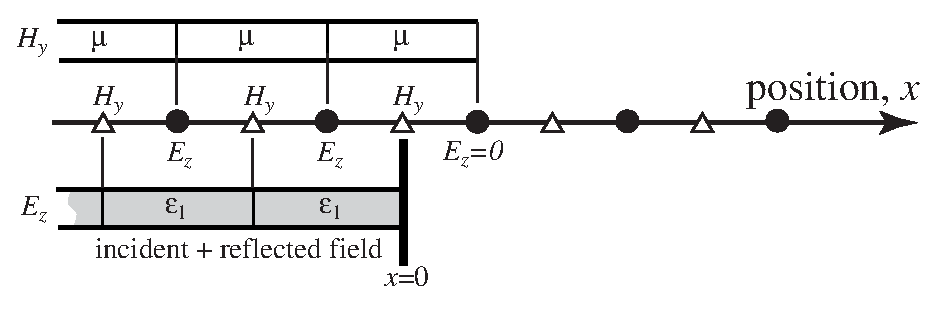
\epsfig{width=4.5in,file=Figures/Fdtd-dispersion/dielectric-pec.eps}
  \end{center}
  \caption{One-dimensional space with a perfect electric conductor
  realized by setting an electric field node to zero.  No fields
  propagate beyond the zeroed node.  The reference point $x=0$ is
  still assumed to coincide with a magnetic-field node.}
  \label{fig:dielectricPEC}
\end{figure}


When a PEC is present there is only one unknown, the reflection
coefficient can be obtained from a single equation since the
transmission coefficient is known {\em a priori}.  This equation is
provided, as before, by the update equation of the magnetic-field node
at the interface.  To this end, \refeq{eq:interfaceEqII} is used with
the transmission coefficient set to zero.  Also, instead of using the
transmitted form of the magnetic field at the interface as was done to
obtain \refeq{eq:usedTrans}, the sum of the incident and reflected
fields is used to obtain:
\begin{equation}
  j\Omega \left(-\frac{1}{\eta_1}+\frac{\Gfdtd}{\eta_1}\right) =
  \frac{1}{\mu\Delx}
     \left(0 - 
           \left[e^{j\tbeta_1\Delx/2} + \Gfdtd e^{-j\tbeta_1\Delx/2}\right]\right).
\end{equation}
Solving for the reflection coefficient yields
\begin{equation}
  \Gfdtd_{\mbox{\scriptsize PEC}} = 
  \frac{j\Omega\mu\Delx - \eta_1 e^{j\tbeta_1\Delx/2}}
       {j\Omega\mu\Delx + \eta_1 e^{-j\tbeta_1\Delx/2}}.
\end{equation}
As was shown in
\refeq{eq:transConversionI}--\refeq{eq:transConversionIV}, the factor
$j\Omega\mu\Delx$ can be expressed in terms of the impedance and a
difference of complex exponentials.  Employing such a conversion
allows the reflection coefficient to be written as
\begin{equation}
  \Gfdtd_{\mbox{\scriptsize PEC}} = -e^{-j\tbeta_1\Delx}.
  \label{eq:fdtdRefPEC}
\end{equation}
Note that the magnitude of the reflection coefficient is unity so that
the entire incident field, regardless of the frequency, is reflected from
the interface.

It appears that the FDTD reflection coefficient for a PEC is
introducing a shift that is not present in the continuous world.
However, this is being a bit unfair to the FDTD method.  The location
of the PEC boundary really corresponds to the electric-field node
that was set to zero.  Thus, one should really think of the PEC
boundary existing at $x=\Delx/2$.

In the continuous world, let us consider a scenario where the origin
is located a distance $\Delx/2$ in front of a PEC boundary.  In that
case the incident and reflected fields must sum to zero at
$x=\Delx/2$, i.e.,
\begin{eqnarray}
  \left.E^{\mbox{\scriptsize inc}}(x) + E^{\mbox{\scriptsize ref}}(x)
  \right|_{x=\Delx/2} &=& 0,\\
  e^{-j\beta_1\Delx/2} + \hat{\Gamma} e^{j\beta_1\Delx/2}  &=& 0.
\end{eqnarray}
Thus, in the continuous world the reflection coefficient is
\begin{equation}
 \hat{\Gamma} = -e^{-j\beta_1\Delx}.
 \label{eq:refContinuousPEC}
\end{equation}
When first comparing \refeq{eq:fdtdRefPEC}
and \refeq{eq:refContinuousPEC} it may appear that in this case the
FDTD reflection coefficient is exact.  However the two differ owing to
the fact that phase constants $\beta_1$ and $\tbeta_1$ are different
in the two domains.

\section{Interface Aligned with an Electric-Field Node}

There are situations which necessitate that a discontinuity in
permittivity be modeled as coinciding with an electric field node.
The permittivity that should be used to either side of the interface
is unambiguous but the permittivity of the node at the interface is
open to question since it is neither in one half-space nor the other.
This scenario was mentioned in Sec.\ \ref{sec:gridInhomogeneities}
where it was suggested that the average permittivity be used for the
node at the interface.  In this section we wish to provide a more
rigorous analysis to justify this permittivity.  For now, let the
permittivity of the node at the interface be $\epsilon_a$ as depicted
in Fig.\ \ref{fig:averageGeom}.  The goal now is to find the reflection or
transmission coefficients for this geometry and find the value of
$\epsilon_a$ which yields the best agreement with the continuous-world
values.

\begin{figure}
  \begin{center}
  \epsfig{width=4.5in,file=Figures/Fdtd-dispersion/half-space-layer.eps}
  \end{center}
  \caption{One-dimensional space with a discontinuity in
  permittivity.  The interface in the continuous world corresponds to
  an electric-field node in the FDTD grid.  The permittivity to the
  left of the interface is $\epsilon_1$ and is $\epsilon_2$ to the
  right.  These values are dictated by those in the continuous world.
  The permittivity of the node at the interface is $\epsilon_a$.}
  \label{fig:averageGeom}
\end{figure}

Although the origin $x=0$ has shifted from that which was assumed in
the previous section, the incident, reflected, and transmitted fields
are still assumed to be given by \refeq{eq:eInc}--\refeq{eq:eTrans} and 
\refeq{eq:hInc}--\refeq{eq:hTrans}.  The electric-field node at the
interface is a member of both half-spaces, i.e., the field is the same
whether considered to be the sum of the incident and reflected field
or simply to be the transmitted field.  This yields a boundary
condition of
\begin{equation}
  1 + \Gfdtd = \Tfdtd.
  \label{eq:elecContinuity}
\end{equation}

Another equation relating the transmission and reflection coefficients
is obtained via the update equation for the electric-field node at the
interface.  Ampere's law evaluated at the interface is
\begin{equation}
  j\epsilon_a\Omega \Tfdtd = \frac{1}{\Delx}
  \left(-\frac{\Tfdtd}{\eta_2} e^{-j\tbeta_2\Delx/2} -
  \left[-\frac{1}{\eta_1} e^{j\tbeta_1\Delx/2} +
         \frac{\Gfdtd}{\eta_1} e^{-j\tbeta_1\Delx/2}\right]
  \right).
\end{equation}
Using \refeq{eq:elecContinuity} $\Tfdtd$ can be replaced with
$1+\Gfdtd$.  Then solving for $\Gfdtd$ yields
\begin{equation}
  \Gfdtd = \frac{\eta_2 e^{j\tbeta_1\Delx/2} - 
                 \eta_1 e^{-j\tbeta_2\Delx/2} - 
                 j\eta_1\eta_2\epsilon_a\Omega\Delx}
                {\eta_2 e^{-j\tbeta_1\Delx/2} +
                 \eta_1 e^{-j\tbeta_2\Delx/2} + 
                 j\eta_1\eta_2\epsilon_a\Omega\Delx}.
  \label{eq:gammaAverage}
\end{equation}
The term $\Omega\Delx$ can be written as
\begin{eqnarray}
  \Omega\Delx &=& \frac{2}{\Delt}
      \sin\!\left(\frac{\omega\Delt}{2}\right)\Delx, \\
  &=& 2c\frac{\Delx}{c\Delt}
      \sin\!\left(\frac{\omega\Delt}{2}\right), \\
  &=& 2c\frac{1}{S_c}
      \sin\!\left(\frac{2\pi c}{\ppw\Delx}\frac{\Delt}{2}\right), \\
  &=& 2c\frac{1}{S_c}
      \sin\!\left(\frac{\pi}{\ppw} S_c\right).
\end{eqnarray}
The conversion of $\omega\Delt/2$ to $\pi S_c/\ppw$ was discussed in
connection with \refeq{eq:lossTerm}.  Using this last form of
$\Omega\Delx$, the third term in the numerator and denominator of
\refeq{eq:gammaAverage} can be written
\begin{eqnarray}
  j\eta_1\eta_2\epsilon_a\Omega\Delx &=&
  j\sqrt{\frac{\mu}{\epsilon_0\epsilon_{r1}}}
   \sqrt{\frac{\mu}{\epsilon_0\epsilon_{r2}}}
  2c\epsilon_0\epsilon_{ra}\frac{1}{S_c}
      \sin\!\left(\frac{\pi}{\ppw} S_c\right), \\
  &=&
  j\frac{\epsilon_{ra}}{\sqrt{\epsilon_{r1}\epsilon_{r2}}}
   \frac{\mu}{\epsilon_0}
  2c\epsilon_0\frac{1}{S_c}
      \sin\!\left(\frac{\pi}{\ppw} S_c\right), \\
  &=&
  j\frac{\epsilon_{ra}}{\sqrt{\epsilon_{r1}\epsilon_{r2}}}
  2\mu c \frac{1}{S_c}
      \sin\!\left(\frac{\pi}{\ppw} S_c\right),
  \label{eq:interfaceTerm}
\end{eqnarray}
where $\epsilon_{ra}$ is the relative permittivity of the node at the
interface.

Assume that the permeability throughout the computational domain is
the permeability of free space so that $\mu c$ in
\refeq{eq:interfaceTerm} can be written $\mu_0
c=\mu_0/\sqrt{\mu_0\epsilon_0} = \sqrt{\mu_0/\epsilon_0} = \eta_0$.
The reflection coefficient \refeq{eq:gammaAverage} can now be written
as
\begin{equation}
  \Gfdtd = \frac{\frac{1}{\sqrt{\epsilon_{r2}}}\eta_0 e^{j\tbeta_1\Delx/2} - 
                \frac{1}{\sqrt{\epsilon_{r1}}}\eta_0 e^{-j\tbeta_2\Delx/2} - 
                j\frac{\epsilon_{ra}}{\sqrt{\epsilon_{r1}\epsilon_{r2}}}
                \eta_0 \frac{2}{S_c}
                \sin\!\left(\frac{\pi}{\ppw} S_c\right)}
              {\frac{1}{\sqrt{\epsilon_{r2}}}\eta_0 e^{-j\tbeta_1\Delx/2} +
                \frac{1}{\sqrt{\epsilon_{r1}}}\eta_0 e^{-j\tbeta_2\Delx/2} + 
                j\frac{\epsilon_{ra}}{\sqrt{\epsilon_{r1}\epsilon_{r2}}}
                \eta_0 \frac{2}{S_c}
                \sin\!\left(\frac{\pi}{\ppw} S_c\right)}.
  \label{eq:gammaAverageI}
\end{equation}
Multiplying numerator and denominator by
$\sqrt{\epsilon_{r1}\epsilon_{r2}}/\eta_0$ yields
\begin{equation}
  \Gfdtd = \frac{\sqrt{\epsilon_{r1}} e^{j\tbeta_1\Delx/2} - 
                 \sqrt{\epsilon_{r2}} e^{-j\tbeta_2\Delx/2} - 
                j \epsilon_{ra} \frac{2}{S_c}
                \sin\!\left(\frac{\pi}{\ppw} S_c\right)}
              {\sqrt{\epsilon_{r1}} e^{-j\tbeta_1\Delx/2} +
               \sqrt{\epsilon_{r2}} e^{-j\tbeta_2\Delx/2} + 
                j\epsilon_{ra} \frac{2}{S_c}
                \sin\!\left(\frac{\pi}{\ppw} S_c\right)}.
  \label{eq:gammaAverageII}
\end{equation}
As is often the case, the expression for a quantity in the FDTD grid
bears little resemblance to that in the continuous world.  However, as
the discretization goes to zero (i.e., $\ppw$ goes to infinity),
\refeq{eq:gammaAverageII} does indeed reduce to the reflection
coefficient in the continuous world.

The first two terms in the numerator and denominator of
\refeq{eq:gammaAverageII} depend on the material constants to either
side of the interface while the third term depends on the permittivity
at the interface, the Courant number, and the number of points per
wavelength (in continuous-world free space).  We now seek the value of
$\epsilon_a$ (or the corresponding relative permittivity
$\epsilon_{ra}$) which minimizes the difference between the reflection
coefficient in the continuous world and the one in the FDTD world.  It
is important to note that in general the FDTD reflection coefficient
in this case is truly complex---there will be a phase shift imparted
that does not exist in the continuous world.

Before going further with the analysis, let us consider an example
with specific parameters and graphically solve for the optimum value
of $\epsilon_a$.  Let $\epsilon_{r1} = 1$, $\epsilon_{r2} = 4$, and
the discretization be 10 points per wavelength.  In this case the
reflection coefficient in the continuous world is $-1/3$ (independent
of frequency).  Figure \ref{fig:refCoefLayer} shows the FDTD
reflection coefficient in the complex plane for various values of
$\epsilon_{ra}$.  The continuous-world result, i.e., the exact result,
is a single point on the negative real axis.  As $\epsilon_{ra}$
varies a curve is obtained in the complex plane which is closest to
the exact value when $\epsilon_{ra}$ is $2.5$ which is the arithmetic
average of $1$ and $4$.  Thus the optimum value for the interface
permittivity is the average of the permittivities to either side.
However, these results are only for a specific discretization and for
one set of permittivities.  Is the average value the optimum one for
all permittivities and discretizations?

\begin{figure}
  \begin{center}
  \epsfig{width=4.5in,file=Figures/Fdtd-dispersion/reflec-re-im.eps}
  \end{center}
  \caption{Curve showing the FDTD reflection coefficient in the
    complex plane as a function of $\epsilon_{ra}$ as $\epsilon_{ra}$
    varies between the relative permittivity to the left of the
    interface ($\epsilon_{ra}=1$) and the relative permittivity to the
    right of the interface ($\epsilon_{ra}=4$).  The value of
    $\epsilon_{ra}$ which minimizes the difference between the FDTD
    reflection coefficient and the exact value of $-1/3$ is the
    average permittivity, i.e., $\epsilon_{ra}=2.5$. }
  \label{fig:refCoefLayer}
\end{figure}

To answer this question, let us return to \refeq{eq:gammaAverage} and
separate the numerator and denominator into real and imaginary parts.
The result is
\begin{equation}
  \Gfdtd = \frac
   {\eta_2\cos(\kappa_1) - \eta_1\cos(\kappa_2) +
     j\left[\eta_2\sin(\kappa_1) + \eta_1\sin(\kappa_2)
      -\eta_1\eta_2\epsilon_a\Omega\Delx\right]}
   {\eta_2\cos(\kappa_1) + \eta_1\cos(\kappa_2) -
     j\left[\eta_2\sin(\kappa_1) + \eta_1\sin(\kappa_2)
      -\eta_1\eta_2\epsilon_a\Omega\Delx\right]}
\end{equation}
where
\begin{eqnarray}
  \kappa_1 &=& \tbeta_1\Delx/2, \\
  \kappa_2 &=& \tbeta_2\Delx/2.
\end{eqnarray}
The continuous-world reflection coefficient is purely real and thus
any imaginary part is an error.  Furthermore, the imaginary part goes
to zero as the discretization goes to zero.  Let us consider just this
imaginary part of the numerator and denominator.  The $\sin(\kappa)$
terms can be related to the $K$ terms which have been used
previously---one merely had to multiply (and divide) by $2/\Delx$.
Thus the imaginary part can be written
\begin{equation}
  \eta_2\frac{2}{\Delx}\sin(\kappa_1)\frac{\Delx}{2} +
  \eta_1\frac{2}{\Delx}\sin(\kappa_2)\frac{\Delx}{2} -
  \eta_1\eta_2\epsilon_a\Omega\Delx
   =
  \eta_1\eta_2\frac{\Delx}{2}\left(\frac{1}{\eta_1}K_1 + 
                    \frac{1}{\eta_2}K_2 -
                    2\epsilon_a\Omega\right).
\end{equation}
From the dispersion relation \ref{eq:fdtdDispersionOneD} we know that
$K_1=\sqrt{\mu\epsilon_1}\Omega$ and $K_2=\sqrt{\mu\epsilon_2}\Omega$.
This allows the imaginary part of the numerator and denominator of the
reflection coefficient to be written
\begin{equation}
  \eta_1\eta_2\frac{\Delx}{2}\Omega
  \left(\epsilon_1 + \epsilon_2 - 2 \epsilon_a\right).
\end{equation}
Setting $\epsilon_a$ equal to $(\epsilon_1+\epsilon_2)/2$ will yield
zero for this imaginary term.  Hence the average permittivity is the
optimum value for all permittivities and discretizations!  Using the
average permittivity yields reflection and transmission coefficients of 
\begin{eqnarray}
  \Gfdtd &=& 
  \frac
   {\eta_2\cos(\kappa_1) - \eta_1\cos(\kappa_2)}
   {\eta_2\cos(\kappa_1) + \eta_1\cos(\kappa_2)}, \\
  \Tfdtd &=& 
  \frac
   {2\eta_2\cos(\kappa_1)}
   {\eta_2\cos(\kappa_1) + \eta_1\cos(\kappa_2)}.
\end{eqnarray}
Note that these equations appear almost identical to those
which pertained to the case of an abrupt interface (i.e., when no
averaging is done and the resulting reflection and transmission
coefficients are \refeq{eq:fdtdRefCoef} and
\refeq{eq:fdtdTransCoef}).  However, these equations differ in the
arguments of the cosine terms and, in fact, it can be shown that the
abrupt boundary is slightly more accurate than the one which is
implemented with the average permittivity at the interface.
Nevertheless, when the situation calls for the interface to coincide
with a tangential electric field, the average permittivity is the
optimum one to use.


\chapter{Two-Dimensional FDTD Simulations\label{chap:multi}}

%\setcounter{page}{1}

\renewcommand{\thefootnote}{\fnsymbol{footnote}}
\footnotetext[2]{Lecture notes by John Schneider.  {\tt
fdtd-multidimensional.tex}}

\section{Introduction}

One of the truly compelling features of the FDTD method is that the
simplicity the method enjoys in one dimension is largely maintained in
higher dimensions.  The complexity of other numerical techniques often
increases substantially as the number of dimensions increases.  With
the FDTD method, if you understand the algorithm in one dimension, you
should have no problem understanding the basic algorithm in two or
three dimensions.  Nevertheless, introducing additional dimensions has
to come at the price of some additional complexity.

This chapter provides details concerning the implementation of
two-dimensional simulations with either the magnetic field or the
electric field orthogonal to the normal to the plane of propagation,
i.e., TM$^z$ or TE$^z$ polarization, respectively.  Multidimensional
simulations require that we think in terms of a multidimensional grid
and thus we require multidimensional arrays to store the fields.
Since we are primarily interested in writing programs in C, we begin
with a discussion of multidimensional arrays in the C language.


%%%%%%%%%%%%%%%%%%%%%%%%%%%%%%%%%%%%%%%%%%%%%%%%%%%%%%%%%%%%%%%%%%%%%%%%%%%
\section{Multidimensional Arrays \label{sec:multiArrays}}

Whether an array is one-, two-, or three-dimensional, it ultimately is
using a block of contiguous memory where each element has a single
address.  The distinction between the different dimensions is
primarily a question of how we want to think about, and access, array
elements.  For higher-dimensional arrays, we want to specify two, or
more, indices to dictate the element of interest.  However, regardless
of the number of indices, ultimately a single address dictates which
memory is being accessed.  The translation of multiple indices to a
single address can be left to the compiler or that translation is
something we can do ourselves.

The code shown in Fragment \ref{frag:twoDDynamic} illustrates how one
can think and work with what is effectively a two-dimensional array
even though the memory allocation is essentially the same as was used
with the one-dimensional array considered in Fragment
\ref{frag:oneDDynamic}.  In Fragment \ref{frag:twoDDynamic} the user
is prompted to enter the desired number of rows and columns which are
stored in {\tt num\_rows} and {\tt num\_columns}, respectively.  In
line \ref{twoDDynamicB} the pointer {\tt ez} is set to the start of a
block of memory which can hold {\tt num\_rows} $\times$ {\tt
num\_columns} doubles.  Thus sufficient space is available to store
the desired number of rows and columns, but this pointer is
dereferenced with a single index (or offset).
\begin{fragment}
Fragment of code demonstrating the construction of a two-dimensional
array. \label{frag:twoDDynamic}
\codemiddle
\begin{lstlisting}
  #define Ez(I, J) ez[(I) * num_columns + (J)]  /*@ \label{twoDDynamicA} @*/
\end{lstlisting}
\mbox{}\hspace{.5in}$\vdots$
\begin{lstlisting}[firstnumber=2]
  double *ez;
  int num_rows, num_columns, m, n;

  printf("Enter the number of row and columns: ");
  scanf("%d %d", &num_rows, &num_columns);

  ez = calloc(num_rows * num_columns, sizeof(double)); /*@ \label{twoDDynamicB} @*/

  for (m=0; m < num_rows; m++)      /*@ \label{twoDDynamicD} @*/
    for (n=0; n < num_columns; n++) 
      Ez(m, n) = m * n;              /*@ \label{twoDDynamicC} @*/
\end{lstlisting}
\end{fragment}

In this code the trick to thinking and working in two dimensions,
i.e., working with two indices instead of one, is the macro which is
shown in line \ref{twoDDynamicA}.  This macro tells the preprocessor
that every time the string {\tt Ez} appears with two arguments---here
the first argument is labeled {\tt I} and the second argument is
labeled {\tt J}---the compiler should translate that to {\tt
ez[(I) * num\_columns + (J)]}.  Note the uppercase {\tt E} in {\tt Ez}
distinguishes this from the pointer {\tt ez}.  {\tt I} and {\tt J} in
the macro are just dummy arguments.  They merely specify how the first
and second arguments should be used in the translated code.  Thus, if
{\tt Ez(2, 3)} appears in the source code, the macro tells the
preprocessor to translate that to {\tt ez[(2) * num\_columns + (3)]}.
In this way we have specified two indices, but the macro translates
those indices into an expression which evaluates to a single number
which represents the offset into a one-dimensional array (the array
{\tt ez}).  Even though {\tt Ez} is technically a macro, we will refer
to it as an array.  Note that, as seen in line \ref{twoDDynamicC},
{\tt Ez}'s indices are enclosed in parentheses, not brackets.

To illustrate this further, assume the user specified that there are
$4$ columns ({\tt num\_columns} is $4$) and $3$ rows.  When the row
number increments by one, that corresponds to moving $4$ locations
forward in memory.  The following shows the arrangement of the
two-dimensional array {\tt Ez(m, n)} where {\tt m} is used for the row
index and {\tt n} is used for the column index.
\begin{center}
\begin{tabular}{l|llll}
    &n=0     & n=1     & n=2     & n=3     \\ \hline
m=0 &Ez(0, 0) & Ez(0, 1) & Ez(0, 2) & Ez(0, 3) \\
m=1 &Ez(1, 0) & Ez(1, 1) & Ez(1, 2) & Ez(1, 3) \\
m=2 &Ez(2, 0) & Ez(2, 1) & Ez(2, 2) & Ez(2, 3)
\end{tabular}
\end{center}
The {\tt Ez} array really corresponds to the one-dimensional {\tt ez}
array.  The macro calculates the index for the {\tt ez} array based on
the arguments (i.e., indices) of the {\tt Ez} array.  The following
shows the same table of values, but in terms of the {\tt ez} array.
\begin{center}
\begin{tabular}{l|llll}
    &n=0     & n=1     & n=2     & n=3     \\ \hline
m=0 &ez[0]   & ez[1]   & ez[2]   & ez[3] \\
m=1 &ez[4]   & ez[5]   & ez[6]   & ez[7] \\
m=2 &ez[8]   & ez[9]   & ez[10]  & ez[11]
\end{tabular}
\end{center}
Again, in this example, when the row is incremented by one, the array
index is incremented by $4$ (which is the number of columns).  This is
due to the fact that we are storing the elements by rows.  An entire
row of values is stored, then the next row, and so on.  Each row
contains {\tt num\_columns} elements.

Instead of storing things by rows, we could have easily employed
``column-centric storage'' where an entire column is stored contiguously.
This would be accomplished by using the macro
\begin{code}
  #define Ez(I, J)   ez[(I) + (J) * num_rows]
\end{code}
This would be used instead of line \ref{twoDDynamicA} in Fragment
\ref{frag:twoDDynamic}.  If this were used, each time the row is
incremented by one the index of {\tt ez} is incremented by one.  If
the column is incremented by one, the index of {\tt ez} would be
incremented by {\tt num\_rows}.  In this case the elements of the {\tt
ez} array would correspond to elements of the {\tt Ez} array as shown
below:
\begin{center}
\begin{tabular}{l|llll}
    &n=0     & n=1     & n=2     & n=3     \\ \hline
m=0 &ez[0]   & ez[3]   & ez[6]   & ez[9] \\
m=1 &ez[1]   & ez[4]   & ez[7]   & ez[10] \\
m=2 &ez[2]   & ez[5]   & ez[8]   & ez[11]
\end{tabular}
\end{center}
Note that when the row index is incremented by one, the index of {\tt
  ez} is also incremented by one.  However, when the column is
incremented by one, the index of {\tt ez} is incremented by $3$, which
is the number of rows.  This type of column-centric storage is used in
FORTRAN.  However, multidimensional arrays in C are generally assumed
to be stored in row-order.  Thus column-centric storage will {\em not}
be considered further and we will use row-centric macros similar to
the one presented in Fragment \ref{frag:twoDDynamic}.

When an array is stored by rows, it is most efficient to access the
array one row at a time---not one column at a time.  Lines
\ref{twoDDynamicD} through \ref{twoDDynamicC} of Fragment
\ref{frag:twoDDynamic} demonstrate this by using two loops to set the
elements of {\tt Ez} to the product of the row and column indices.
The inner loop is over the row and the outer loop sets the column.
This is more efficient than if these loops were interchanged (although
there is likely to be no difference for small arrays).  This is a
consequence of the way memory is stored both on the disk and in the
CPU cache.  

Memory is accessed in small chunks known as pages.  If the CPU needs
access to a certain variable that is not already in the cache, it will
generate a page fault (and servicing a page fault takes more time than
if the variable were already in the cache).  When the page gets to the
cache it contains more than just the variable the CPU wanted---it
contains other variables which were stored in memory adjacent to the
variable of interest (the page may contain many variables).  If the
subsequent CPU operations involve a variable that is already in the
cache, that operation can be done very quickly.  It is most likely
that that variable will be in the cache, and the CPU will not have to
generate a page fault, if that variable is adjacent in memory to the
one used in the previous operation.  Thus, assuming row-centric
storage, working with arrays row-by-row is the best way to avoid
needless page faults.

It is important to note that we should not feel constrained to
visualize our arrays in terms of the standard way in which arrays are
displayed!  Typically two-dimensional arrays are displayed in a table
with the first element in the upper, left-hand corner of the table.
The first index gives the row number and the second index gives the
column number.  FDTD simulations are modeling a physical space, not a
table of numbers.  In two dimensions we will be concerned with spatial
dimensions $x$ and $y$.  It is convention to give the $x$ location as
the first argument and the $y$ location as the second argument, i.e.,
$E_z(x,y)$.  It is also often the case that it is convenient to think
of the lower left-hand corner of some finite rectangular region of
space as the origin.  It is perfectly acceptable to use the array
mechanics which have been discussed so far but to imagine them
corresponding to an arrangement in space which corresponds to our
usual notion of variation in the $x$ and $y$ directions.  So, for
example, in the case of a $3$ by $4$ array, one can visualize the
nodes as being arranged in the following way:
\begin{center}
\begin{tabular}{l|lllll|lll}
n=3 &Ez(0,3) & Ez(1,3) & Ez(2,3) &&
       n=3   &ez[3]&ez[7]&ez[11]\\
n=2 &Ez(0,2) & Ez(1,2) & Ez(2,2) &&
       n=2   &ez[2]&ez[6]&ez[10]\\
n=1 &Ez(0,1) & Ez(1,1) & Ez(2,1) &
\hspace{.2in}$\Longleftrightarrow$\hspace{.2in}\mbox{}&
       n=1   &ez[1]&ez[5]&ez[9]\\
n=0 &Ez(0,0) & Ez(1,0) & Ez(2,0) &&
       n=0   &ez[0]&ez[4]&ez[8]\\\cline{1-4}\cline{6-9}
    &m=0     & m=1     & m=2     &&
             &m=0  &m=1  &m=2  \\
\end{tabular}
\end{center}
Nothing has changed in terms of the implementation of the macro to
realize this two-dimensional array---the only difference is the way
the elements have been displayed.  The depiction here is natural when
thinking in terms of variations in $x$ and $y$, where the first index
corresponds to $x$ and the second index corresponds to $y$.  The
previous depiction was natural to the way most people discuss tables
of data.  Regardless of how we think of the arrays, it is still true
that the second index is the one that should vary most rapidly in the
case of nested loops (i.e., one should strive to have consecutive
operations access consecutive elements in memory).

As mentioned in Sec.\ \ref{sec:memAllocation}, it is always best to
check that an allocation of memory was successful.  If {\tt calloc()}
is unable to allocated the requested memory, it will return {\tt
NULL}.  After every allocation we could add code to check that the
request was successful.  However, as we did in one-dimension, a better
approach is again offered with the use of macros.  Fragment
\ref{frag:allocMacro2D} shows a macro that can be used to allocate
memory for a two-dimensional array.

\begin{fragment}
Macro for allocating memory for a two-dimensional array. 
\label{frag:allocMacro2D}
\codemiddle
\begin{lstlisting}
#define ALLOC_2D(PNTR, NUMX, NUMY, TYPE)                        \
    PNTR = (TYPE *)calloc((NUMX) * (NUMY), sizeof(TYPE));       \
    if (!PNTR) {                                                \
      perror("ALLOC_2D");                                       \
      fprintf(stderr,                                           \
          "Allocation failed for " #PNTR ".  Terminating...\n");\
      exit(-1);                                                 \
    }
\end{lstlisting}
\end{fragment}
The macro {\tt ALLOC\_2D()} is similar to {\tt ALLOC\_1D()}, which was
presented in Fragment\ \ref{frag:allocMacro}, except it takes four
arguments instead of three.  The first argument is a pointer, the
second is the number of rows, the third is the number of columns, and
the fourth is the data type.  As an example of how this macro could be
used, line \ref{twoDDynamicB} of Fragment
\ref{frag:twoDDynamic} could be replaced with
\begin{code}
  ALLOC_2D(ez, num_rows, num_columns, double);
\end{code}

%%%%%%%%%%%%%%%%%%%%%%%%%%%%%%%%%%%%%%%%%%%%%%%%%%%%%%%%%%%%%%%%%%%%%%%%%%%
\section{Two Dimensions: TM$^z$ Polarization \label{sec:tmzPolarization}}

The one-dimensional problems considered thus far assumed a non-zero
$z$ component of the electric field and variation only in the $x$
direction.  This required the existence of a non-zero $y$ component of
the magnetic field.  Here the field is assumed to vary in both the $x$
and $y$ directions, but not the $z$ direction.  From the outset we
will include the possibility of a magnetic conductivity $\sigma_m$.
With these assumptions Faraday's law becomes
\begin{equation}
  -\sigma_m\Hvec -\mu \frac{\partial \Hvec}{\partial t} =
  \nabla \times \Evec =
  \left|
  \begin{array}{ccc}
     \unitvec{x} & \unitvec{y} & \unitvec{z} \\
     \frac{\partial}{\partial x} & \frac{\partial}{\partial y}  & 0 \\
     0 & 0 & E_z
  \end{array}
  \right|
  = \unitvec{x}\frac{\partial E_z}{\partial y}
   -\unitvec{y}\frac{\partial E_z}{\partial x}.
 \label{eq:faradayTMz}
\end{equation}
Since the right-hand side only has non-zero components in the $x$ and
$y$ directions, the time-varying components of the magnetic field can
only have non-zero $x$ and $y$ components (we are not concerned with
static fields nor a rather pathological case where the magnetic
current $\sigma_m\Hvec$ cancels the time-varying field
$\partial\Hvec/\partial t$).  The magnetic field is transverse to the
$z$ direction and hence this is designated the TM$^z$ case.  Ampere's
law becomes
\begin{equation}
  \sigma \Evec + \epsilon \frac{\partial \Evec}{\partial t} =
  \nabla \times \Hvec =
  \left|
  \begin{array}{ccc}
     \unitvec{x} & \unitvec{y} & \unitvec{z} \\
     \frac{\partial}{\partial x} & \frac{\partial}{\partial y}  & 0 \\
     H_x & H_y & 0
  \end{array}
  \right|
  = \unitvec{z}\left(\frac{\partial H_y}{\partial x}
                    -\frac{\partial H_x}{\partial y}\right).
 \label{eq:ampereTMz}
\end{equation}

The scalar equations obtained from \refeq{eq:faradayTMz} and
\refeq{eq:ampereTMz} are
\begin{eqnarray}
  -\sigma_m H_x - \mu\frac{\partial H_x}{\partial t} &=&
    \frac{\partial E_z}{\partial y},  \label{eq:faradayTMzX}
  \\
  \sigma_m H_y + \mu\frac{\partial H_y}{\partial t} &=&
    \frac{\partial E_z}{\partial x}, \label{eq:faradayTMzY}
  \\
  \sigma E_z + \epsilon\frac{\partial E_z}{\partial t} &=&
     \frac{\partial H_y}{\partial x}
    -\frac{\partial H_x}{\partial y}. \label{eq:ampereTMzZ}
\end{eqnarray}
Note that, ignoring the conduction terms for a moment, the temporal
derivative of the magnetic field is related to the spatial derivative
of the electric field and vice versa.  The only difference from the
one-dimensional case is the additional field component $H_x$ and 
the derivatives in the $y$ direction.

Space-time is now discretized so that
\refeq{eq:faradayTMzX}--\refeq{eq:ampereTMzZ} can be expressed in
terms of finite-differences.  From these difference equations the future
fields can be expressed in terms of past fields.  Following the
notation used in Sec.\ \ref{sec:update}, the following notation will be
used: 
\begin{eqnarray}
  H_x(x,y,t) \!&=&\! H_x(m\Delx, n\Dely, q\Delt) =
          \fdtd{H_x}{m,n}{q},  \\
  H_y(x,y,t) \!&=&\! H_y(m\Delx, n\Dely, q\Delt) =
          \fdtd{H_y}{m,n}{q},  \\
  E_z(x,y,t) \!&=&\! E_z(m\Delx, n\Dely, q\Delt) = \fdtd{E_z}{m,n}{q}.
\end{eqnarray}
As before, the index $m$ corresponds to the spatial step in the $x$
direction while the index $q$ corresponds to the temporal step.
Additionally the index $n$ represents the spatial step in the $y$
direction.  The spatial step sizes in the $x$ and $y$ directions are
$\Delx$ and $\Dely$, respectively (these need not be equal).

In order to obtain the necessary update-equations, each of the field
components must be staggered in space.  However, it is not necessary
to stagger all the field components in time.  The electric field must
be offset from the magnetic field, but the magnetic field components
do not need to be staggered relative to each other---all the magnetic
field components can exist at the same time.  A suitable spatial
staggering of the electric and magnetic field components is shown in
Fig.\ \ref{fig:tmzGrid}.

\begin{figure}
  \begin{center}
  \epsfig{width=5in,file=Figures/Fdtd-multidimensional/tmz-fdtd-grid.eps}
\end{center} \caption{Spatial arrangement of electric- and
  magnetic-field nodes for TM$^z$ polarization.  The electric-field
  nodes are shown as circles and the magnetic-field nodes as squares
  with a line that indicates the orientation of the field component.
  The somewhat triangularly shaped dashed lines indicate groupings of
  nodes that have the same array indices.  For example, in the lower
  left corner of the grid all the nodes would have indices in a
  computer program of $(m=0,n=0)$.  In this case the spatial offset of
  the fields is implicitly understood.  This grouping is repeated
  throughout the grid.  However, groups at the top of the grid lack an
  $H_x$ node and groups at the right edge lack an $H_y$ node.  The
  diagram at the bottom left of the figure indicates nodes with their
  offsets given explicitly in the spatial arguments whereas the
  diagram at the bottom right indicates how the same nodes would be
  specified in a computer program where the offsets are understood
  implicitly.}  \label{fig:tmzGrid}
\end{figure}

When we say the dimensions of a TM$^z$ grid is $M\times N$, that
corresponds to the dimensions of the $E_z$ array.  We will ensure the
grid is terminated such that there are electric-field nodes on the
edge of the grid.  Thus, the $H_x$ array would by $M\times (N-1)$
while the $H_y$ array would be $(M-1)\times N$.

In the arrangement of nodes shown in Fig.\ \ref{fig:tmzGrid} we will
assume the electric field nodes fall at integer spatial steps and the
magnetic field nodes are offset a half spatial step in either the $x$
or $y$ direction.  As with one dimension, the electric field is
assumed to exist at integer multiples of the temporal step while both
magnetic fields components are offset a half time-step from the
electric fields.  With this arrangement in mind,
the finite difference approximation of \refeq{eq:faradayTMzX} expanded
about the space-time point $(m\Delx,(n+1/2)\Dely,q\Delt)$ is
\begin{eqnarray}
  \lefteqn{\hspace{-.4in}
    -\sigma_m \frac{\fdtdh{H_x}{m,n+\half}{q+\half} +
                 \fdtdh{H_x}{m,n+\half}{q-\half}}{2}
    -\mu\frac{\fdtdh{H_x}{m,n+\half}{q+\half} -
            \fdtdh{H_x}{m,n+\half}{q-\half}}{\Delt}
   =} \nonumber \\
  & &  \hspace{3.3in}
   \frac{\fdtd{E_z}{m,n+1}{q}-\fdtd{E_z}{m,n}{q}}{\Dely}.
  \label{eq:fdtdTMzX}
\end{eqnarray}
This can be solved for the future value
$\fdtdh{H_x}{m,n+\half}{q+\half}$ in terms of the ``past''
values.  The resulting update equation is
\begin{equation}
  \fdtdh{H_x}{m,n+\half}{q+\half} =
  \frac{1-\frac{\sigma_m\Delt}{2\mu}}{1+\frac{\sigma_m\Delt}{2\mu}}
  \fdtdh{H_x}{m,n+\half}{q-\half} -
  \frac{1}{1+\frac{\sigma_m\Delt}{2\mu}}
   \frac{\Delt}{\mu\Dely}\left(\fdtd{E_z}{m,n+1}{q}-
                               \fdtd{E_z}{m,n}{q}\right).
  \label{eq:updateHxTMz}
\end{equation}
As was the case in one dimension, the material parameters $\mu$ and
$\sigma_m$ are those which pertain at the given evaluation point.

The update equation for the $y$ component of the magnetic field is
obtained by the finite-difference approximation of
\refeq{eq:faradayTMzY} expanded about the space-time point
$((m+1/2)\Delx,n\Dely,q\Delt)$.  The resulting equation is 
\begin{equation}
  \fdtdh{H_y}{m+\half,n}{q+\half} =
  \frac{1-\frac{\sigma_m\Delt}{2\mu}}{1+\frac{\sigma_m\Delt}{2\mu}}
  \fdtdh{H_y}{m+\half,n}{q-\half} + 
  \frac{1}{1+\frac{\sigma_m\Delt}{2\mu}}
   \frac{\Delt}{\mu\Delx}\left(\fdtd{E_z}{m+1,n}{q}-
                               \fdtd{E_z}{m,n}{q}\right).
  \label{eq:updateHyTMz}
\end{equation}
Again, the material parameters $\mu$ and $\sigma_m$ are those which
pertain at the given evaluation point.  Note that $H_y$ nodes are
offset in space from $H_x$ nodes.  Hence the $\mu$ and $\sigma_m$
appearing in \refeq{eq:updateHxTMz} and \refeq{eq:updateHyTMz} are not
necessarily the same even when $m$ and $n$ are the same.

The electric-field update equation is obtained via the finite-difference
approximation of \refeq{eq:ampereTMzZ} expanded about
$(m\Delx,n\Dely,(q+1/2)\Delt)$:
\begin{eqnarray}
  \fdtd{E_z}{m,n}{q+1} &=&
  \frac{1-\frac{\sigma\Delt}{2\epsilon}}{1+\frac{\sigma\Delt}{2\epsilon}}
  \fdtd{E_z}{m,n}{q} + 
  \frac{1}{1+\frac{\sigma\Delt}{2\epsilon}}
  \left(
    \frac{\Delt}{\epsilon\Delx}
    \left\{
      \fdtdh{H_y}{m+\half,n}{q+\half} - \fdtdh{H_y}{m-\half,n}{q+\half}
    \right\}\right.
 \nonumber\\
  && \hspace{1.2in} \mbox{} - 
	\left.
    \frac{\Delt}{\epsilon\Dely}
    \left\{
      \fdtdh{H_x}{m,n+\half}{q+\half} - \fdtdh{H_x}{m,n-\half}{q+\half}
    \right\}
  \right).
\end{eqnarray}

A uniform grid is one in which the spatial step size is the same in
all directions.  Assuming a uniform grid such that
$\Delx=\Dely=\delta$, we define the following quantities
\begin{eqnarray}
\chxh(m,n+1/2) &=&
  \left.
    \frac{1-\frac{\sigma_m\Delt}{2\mu}}{1+\frac{\sigma_m\Delt}{2\mu}}
  \right|_{m\delta,(n+1/2)\delta}, \\
\chxe(m,n+1/2) &=&
  \left.
    \frac{1}{1+\frac{\sigma_m\Delt}{2\mu}}\frac{\Delt}{\mu\delta}
  \right|_{m\delta,(n+1/2)\delta}, \\
\chyh(m+1/2,n) &=&
  \left.
    \frac{1-\frac{\sigma_m\Delt}{2\mu}}{1+\frac{\sigma_m\Delt}{2\mu}}
  \right|_{(m+1/2)\delta,n\delta}, \\
\chye(m+1/2,n) &=&
  \left.
    \frac{1}{1+\frac{\sigma_m\Delt}{2\mu}}\frac{\Delt}{\mu\delta}
  \right|_{(m+1/2)\delta,n\delta}, \\
\ceze(m,n) &=& 
  \left.
  \frac{1-\frac{\sigma\Delt}{2\epsilon}}{1+\frac{\sigma\Delt}{2\epsilon}}
  \right|_{m\delta,n\delta}, \\
\cezh(m,n) &=& 
  \left.
  \frac{1}{1+\frac{\sigma\Delt}{2\epsilon}}
    \frac{\Delt}{\epsilon\delta}
  \right|_{m\delta,n\delta}.
\end{eqnarray}
These quantities appear in the update equations and employ the
following naming convention: the first letter identifies the quantity
as a constant which does not vary in time (one can also think of this
$C$ as representing the word coefficient), the next two letters
indicate the field being updated, and the last letter indicates the
type of field this quantity multiplies.  For example, $\chxh$
appears in the update equation for $H_x$ and it multiples the previous
value of the magnetic field.  On the other hand, $\chxe$, which
also appears in the update equation for $H_x$, multiplies the electric
fields.

To translate these update equations into a form that is suitable for
use in a computer program, we follow the approach that was used in
one dimension: explicit references to the time step are dropped and
the spatial offsets are understood.  As illustrated in Fig.\
\ref{fig:tmzGrid}, an $H_y$ node is assumed to be a half spatial step
further in the $x$ direction than the corresponding $E_z$ node with
the same indices.  Similarly, an $H_x$ node is assumed to be a half
spatial step further in the $y$ direction than the corresponding $E_z$
node with the same indices.  Thus, in C, the update equations could be
written
\begin{code}
  Hx(m, n) = Chxh(m, n) * Hx(m, n) - 
     Chxe(m, n) * (Ez(m, n + 1) - Ez(m, n));
  Hy(m, n) = Chyh(m, n) * Hy(m, n) + 
     Chye(m, n) * (Ez(m + 1, n) - Ez(m, n));
  Ez(m, n) = Ceze(m, n) * Ez(m, n) + 
     Cezh(m, n) * ((Hy(m, n) - Hy(m - 1, n)) - (Hx(m, n) - Hx(m, n - 1)));
\end{code}
The reason that the ``arrays'' appearing in these equations start with
an uppercase letter and use parentheses (instead of two pairs of
brackets that would be used with traditional two-dimensional arrays
in C) is because these terms are actually macros consistent with the
usage described in Sec.\ \ref{sec:multiArrays}.  In order for these
equations to be useful, they have to be contained within loops that
cycle over the spatial indices and these loops must themselves be
contained within a time-stepping loop.  Additional considerations are
initialization of the arrays, the introduction of energy, and
termination of the grid.  This issues are covered in the following sections.

\section{TM$^z$ Example}

To illustrate the simplicity of the FDTD method in two dimensions, let
us consider a simulation of a TM$^z$ grid which is $101$ nodes by $81$
nodes and filled with free space.  The grid will be terminated on
electric field nodes which will be left at zero (so that the
simulation is effectively of a rectangular resonator with PEC walls).
A Ricker wavelet with $20$ points per wavelength at its most energetic
frequency is hardwired to the electric-field node at the center of the
grid.  

Before we get to the core of the code, we are now at a point where it
is convenient to split the main header file into multiple header
files: one defining the {\tt Grid} structure, one defining various
macros, one giving the allocation macros, and one providing the
function prototypes.  Not all the ``{\tt .c}'' files need to include
each of these header files.

The arrangement of the code is shown in Fig.\ \ref{fig:filesTmZ}.  In
this figure the header files {\tt fdtd-grid1.h}, {\tt
fdtd-alloc1.h}, {\tt fdtd-macro-tmz.h}, and {\tt fdtd-proto1.h} are
shown in a single box but they exist as four separate files (as will
be shown below).

\begin{figure}
  \begin{center}
  \epsfig{width=4.1in,file=Figures/Fdtd-multidimensional/tmzdemo1-files.eps}
  \end{center} \caption{The files associated with a simple TM$^z$
  simulation with a hard source at the center of the grid.  The four
  header files with an {\tt fdtd-} prefix are lumped into a single
  box.  Not all these files are included in each of the files to which
  this box is linked.  See the code for the specifics related to the
  inclusion of these files. }
  \label{fig:filesTmZ}
\end{figure}

The contents of {\tt fdtd-grid1.h} are shown in Program
\ref{pro:fdtdgrid1h}.  The {\tt Grid} structure, which begins on line
\ref{fdtdgrid1hB}, now has elements for any of the possible electric
or magnetic field components as well as their associated coefficient
arrays.  Note that just because all the pointers are declared, they do
not have to be used or point to anything useful.  The {\tt Grid}
structure shown here could be used for a 1D simulation---it provides
elements for everything that was needed to do a 1D simulation---but
most of the pointers would be unused, i.e., those elements that
pertain to anything other than a 1D simulation would be ignored.

The way we will distinguish between what different grids are being
used for is by setting the ``{\tt type}'' field of the grid.  Note
that line \ref{fdtdgrid1hA} creates a {\tt GRIDTYPE} enumeration.
This command merely serves to set the value of {\tt oneDGrid} to zero,
the value of {\tt teZGrid} to one, and the value of {\tt tmZGrid} to
two.  (The value of {\tt threeDGrid} would be three, but we are not
yet concerned with three-dimensional grids.)  A {\tt Grid} will have
its {\tt type} set to one of these values.  Functions can then check
the {\tt type} and act accordingly.

\begin{program}
{\tt fdtd-grid1.h}  Contents of the header file that defines the {\tt
Grid} structure.  This structure now contains pointers for each of the
possible field values.  However, not all these pointers would be used
for any particular grid.  The pointers that are meaningful would be
determined by the ``{\tt type}'' of the grid.  The {\tt type} takes on
one of the values of the {\tt GRIDTYPE} enumeration.
\label{pro:fdtdgrid1h}
\codemiddle
\begin{lstlisting}
#ifndef _FDTD_GRID1_H
#define _FDTD_GRID1_H

enum GRIDTYPE {oneDGrid, teZGrid, tmZGrid, threeDGrid}; /*@ \label{fdtdgrid1hA} @*/

struct Grid {                 /*@ \label{fdtdgrid1hB} @*/
  double *hx, *chxh, *chxe;
  double *hy, *chyh, *chye;
  double *hz, *chzh, *chze;
  double *ex, *cexe, *cexh;
  double *ey, *ceye, *ceyh;
  double *ez, *ceze, *cezh;
  int sizeX, sizeY, sizeZ;
  int time, maxTime;
  int type;
  double cdtds;
};

typedef struct Grid Grid;

#endif
\end{lstlisting}
\end{program}

The contents of {\tt fdtd-alloc1.h} are shown in Program
\ref{pro:fdtdalloc1h}.  This header file merely provides the
memory-allocation macros that have been discussed previously.

\begin{program}
{\tt fdtd-alloc1.h} Contents of the header file that defines the
memory allocation macros suitable for 1D and 2D arrays.
\label{pro:fdtdalloc1h}
\codemiddle
\begin{lstlisting}
#ifndef _FDTD_ALLOC1_H
#define _FDTD_ALLOC1_H

#include <stdio.h>
#include <stdlib.h>

/* memory allocation macros */
#define ALLOC_1D(PNTR, NUM, TYPE)                               \
    PNTR = (TYPE *)calloc(NUM, sizeof(TYPE));                   \
    if (!PNTR) {                                                \
      perror("ALLOC_1D");                                       \
      fprintf(stderr,                                           \
          "Allocation failed for " #PNTR ".  Terminating...\n");\
      exit(-1);                                                 \
    }

#define ALLOC_2D(PNTR, NUMX, NUMY, TYPE)                            \
    PNTR = (TYPE *)calloc((NUMX) * (NUMY), sizeof(TYPE));           \
    if (!PNTR) {                                                    \
      perror("ALLOC_2D");                                           \
      fprintf(stderr,                                               \
              "Allocation failed for " #PNTR ".  Terminating...\n");\
      exit(-1);                                                     \
    }

#endif
\end{lstlisting}
\end{program}

The contents of {\tt fdtd-macro-tmz.h} are shown in Program
\ref{pro:fdtdmacrotmzh}.  This file provides the macros used to access
the field arrays and elements of a pointer to a {\tt Grid} structure.
Thus far all the macros we have used assumed the {\tt Grid} pointer
was called {\tt g}.  The macros provided in lines
\ref{fdtdmacrotmzHA}--\ref{fdtdmacrotmzHB} no longer make this
assumption.  Instead, one specifies the name of the pointer as the
first argument.  To this point in our code there is no need for this
added degree of freedom.  We only considered code that has one pointer
to a {\tt Grid} and we have consistently named it {\tt g}.  However,
as we will see when we discuss the TFSF boundary, it is convenient to
have the ability to refer to different grids.

The macros in lines \ref{fdtdmacrotmzHC}--\ref{fdtdmacrotmzHD} do
assume the {\tt Grid} pointer is named {\tt g}.  These macros are
actually defined in terms of the first set of macros where the first
argument has been set to {\tt g}.  Note that although we are
discussing a 2D TM$^z$ problem, this file still provides macros that
can be used for a 1D array.  Again, we will see, when we implement a
2D TFSF boundary, that there are valid reasons for doing this.  Since
any function that is using these macros will also need to know about a
{\tt Grid} structure, line \ref{fdtdmacrotmzHE} ensures that the {\tt
  fdtd-grid1.h} header file is also included.

\begin{program}
{\tt fdtd-macro-tmz.h} Header file providing macros suitable for
accessing the elements and arrays of either a 1D or 2D {\tt Grid}.
There are two distinct sets of macros.  The first set takes an
argument that speficies the name of the pointer to the {\tt Grid}
structure.  The second set assumes the name of the pointer is {\tt g}.
\label{pro:fdtdmacrotmzh}
\codemiddle
\begin{lstlisting}
#ifndef _FDTD_MACRO_TMZ_H
#define _FDTD_MACRO_TMZ_H

#include "fdtd-grid1.h"    /*@ \label{fdtdmacrotmzHE} @*/

/* macros that permit the "Grid" to be specified */
/* one-dimensional grid */
#define Hy1G(G, M)      G->hy[M]   /*@ \label{fdtdmacrotmzHA} @*/
#define Chyh1G(G, M)    G->chyh[M]
#define Chye1G(G, M)    G->chye[M]

#define Ez1G(G, M)      G->ez[M]
#define Ceze1G(G, M)    G->ceze[M]
#define Cezh1G(G, M)    G->cezh[M]

/* TMz grid */
#define HxG(G, M, N)     G->hx[(M) * (SizeYG(G)-1) + (N)]
#define ChxhG(G, M, N) G->chxh[(M) * (SizeYG(G)-1) + (N)]
#define ChxeG(G, M, N) G->chxe[(M) * (SizeYG(G)-1) + (N)]

#define HyG(G, M, N)     G->hy[(M) * SizeYG(G) + (N)]
#define ChyhG(G, M, N) G->chyh[(M) * SizeYG(G) + (N)]
#define ChyeG(G, M, N) G->chye[(M) * SizeYG(G) + (N)]

#define EzG(G, M, N)     G->ez[(M) * SizeYG(G) + (N)]
#define CezeG(G, M, N) G->ceze[(M) * SizeYG(G) + (N)]
#define CezhG(G, M, N) G->cezh[(M) * SizeYG(G) + (N)]

#define SizeXG(G)        G->sizeX
#define SizeYG(G)        G->sizeY
#define SizeZG(G)        G->sizeZ
#define TimeG(G)         G->time
#define MaxTimeG(G)      G->maxTime
#define CdtdsG(G)        G->cdtds
#define TypeG(G)         G->type     /*@ \label{fdtdmacrotmzHB} @*/

/* macros that assume the "Grid" is "g" */
/* one-dimensional grid */
#define Hy1(M)      Hy1G(g, M)     /*@ \label{fdtdmacrotmzHC} @*/
#define Chyh1(M)    Chyh1G(g, M)
#define Chye1(M)    Chye1G(g, M)

#define Ez1(M)      Ez1G(g, M)
#define Ceze1(M)    Ceze1G(g, M)
#define Cezh1(M)    Cezh1G(g, M)

/* TMz grid */
#define Hx(M, N)   HxG(g, M, N)
#define Chxh(M, N) ChxhG(g, M, N)
#define Chxe(M, N) ChxeG(g, M, N) 

#define Hy(M, N)   HyG(g, M, N)
#define Chyh(M, N) ChyhG(g, M, N)
#define Chye(M, N) ChyeG(g, M, N)

#define Ez(M, N)   EzG(g, M, N)
#define Ceze(M, N) CezeG(g, M, N) 
#define Cezh(M, N) CezhG(g, M, N) 

#define SizeX        SizeXG(g)
#define SizeY        SizeYG(g)
#define SizeZ        SizeZG(g)
#define Time         TimeG(g)
#define MaxTime      MaxTimeG(g)
#define Cdtds        CdtdsG(g)
#define Type         TypeG(g)       /*@ \label{fdtdmacrotmzHD} @*/

#endif   /* matches #ifndef _FDTD_MACRO_TMZ_H */
\end{lstlisting}
\end{program}

Finally, the contents of {\tt fdtd-proto1.h} are shown in Program
\ref{pro:fdtdproto1}.  This file provides the prototypes for the
various functions associated with the simulation.  Since a pointer to
a {\tt Grid} appears as an argument to these functions, any file that
includes this header will also need to include {\tt fdtd-grid1.h} as
is done in line \ref{fdtdproto1A}.

\begin{program}
{\tt fdtd-proto1.h} Header file providing the function prototypes.
\label{pro:fdtdproto1}
\codemiddle
\begin{lstlisting}
#ifndef _FDTD_PROTO1_H
#define _FDTD_PROTO1_H

#include "fdtd-grid1.h"  /*@ \label{fdtdproto1A} @*/

/* Function prototypes */
void gridInit(Grid *g);

void snapshotInit2d(Grid *g);
void snapshot2d(Grid *g);

void updateE2d(Grid *g);
void updateH2d(Grid *g);

#endif
\end{lstlisting}
\end{program}

The file {\tt tmzdemo1.c}, which contains the {\tt main()} function,
is shown in Program \ref{pro:tmzdemo1}.  The program begins with the
inclusion of the necessary header files.  Note that only three of the
four {\tt fdtd-} header files are explicitly included.  However, both
the header files {\tt fdtd-macro-tmz.h} and {\tt fdtd-proto1.h} ensure
that the ``missing'' file, {\tt fdtd-grid1.h}, is included.

Fields are introduced into the grid by hardwiring the value of an
electric-field node as shown in line \ref{tmzdemo1A}.  Because the
source function is used in {\tt main()}, the header file {\tt ezinc.h}
had to be included in this file.  Other than those small changes, this
program looks similar to many of the 1D programs which we have
previously considered.

\begin{program}
{\tt tmzdemo1.c}
FDTD implementation of a TM$^z$ grid with a Ricker wavelet source at
the center of the grid.  No ABC have been implemented so the
simulation is effectively of a resonator.
\label{pro:tmzdemo1}
\codemiddle
\begin{lstlisting}
/* TMz simulation with Ricker source at center of grid. */

#include "fdtd-alloc1.h"
#include "fdtd-macro-tmz.h"
#include "fdtd-proto1.h"
#include "ezinc.h"

int main()
{
  Grid *g;

  ALLOC_1D(g, 1, Grid); // allocate memory for Grid

  gridInit(g);        // initialize the grid
  ezIncInit(g);
  snapshotInit2d(g);  // initialize snapshots

  /* do time stepping */
  for (Time = 0; Time < MaxTime; Time++) {
    updateH2d(g);     // update magnetic field
    updateE2d(g);     // update electric field
    Ez(SizeX / 2, SizeY / 2) = ezInc(Time, 0.0); // add a source /*@ \label{tmzdemo1A} @*/
    snapshot2d(g);    // take a snapshot (if appropriate)
  } // end of time-stepping

  return 0;
}
\end{lstlisting}
\end{program}

The contents of {\tt gridtmz.c}, which contains the grid
initialization function {\tt gridInit()}, is shown in Program
\ref{pro:gridtmz}.  On line \ref{gridtmzA} the type of grid is
defined.  This is followed by statements which set the size of the
grid, in both the $x$ and $y$ directions, the duration of the
simulation, and the Courant number.  Then, on lines \ref{gridtmzB}
through \ref{gridtmzC}, space is allocated for the field arrays and
their associated coefficients array.  Note that although the $E_z$
array is {\tt SizeX}$\times${\tt SizeY}, $H_x$ is {\tt
  SizeX}$\times(\mbox{\tt SizeY}-1)$, and $H_y$ is $(\mbox{\tt
  SizeX}-1)\times${\tt SizeY}.  The remainder of the program merely
sets the coefficient arrays.  Here there is no need to include the
header file {\tt fdtd-proto1.h} since this function does not call any
of the functions listed in that file.

\begin{program}
{\tt gridtmz.c} Grid initialization function for a TM$^z$ simulation.
Here the grid is simply homogeneous free space.
\label{pro:gridtmz}
\codemiddle
\begin{lstlisting}
#include "fdtd-macro-tmz.h"
#include "fdtd-alloc1.h"
#include <math.h>

void gridInit(Grid *g) {
  double imp0 = 377.0;
  int mm, nn;

  Type = tmZGrid;                          /*@ \label{gridtmzA} @*/
  SizeX = 101;             // x size of domain
  SizeY = 81;              // y size of domain
  MaxTime = 300;           // duration of simulation
  Cdtds = 1.0 / sqrt(2.0); // Courant number

  ALLOC_2D(g->hx,   SizeX, SizeY - 1, double);  /*@ \label{gridtmzB} @*/
  ALLOC_2D(g->chxh, SizeX, SizeY - 1, double);
  ALLOC_2D(g->chxe, SizeX, SizeY - 1, double);
  ALLOC_2D(g->hy,   SizeX - 1, SizeY, double);
  ALLOC_2D(g->chyh, SizeX - 1, SizeY, double);
  ALLOC_2D(g->chye, SizeX - 1, SizeY, double);
  ALLOC_2D(g->ez,   SizeX, SizeY, double);
  ALLOC_2D(g->ceze, SizeX, SizeY, double);
  ALLOC_2D(g->cezh, SizeX, SizeY, double);    /*@ \label{gridtmzC} @*/
 
  /* set electric-field update coefficients */
  for (mm = 0; mm < SizeX; mm++)
    for (nn = 0; nn < SizeY; nn++) {
      Ceze(mm, nn) = 1.0;
      Cezh(mm, nn) = Cdtds * imp0;
    }

  /* set magnetic-field update coefficients */
  for (mm = 0; mm < SizeX; mm++)
    for (nn = 0; nn < SizeY - 1; nn++) {
      Chxh(mm, nn) = 1.0;
      Chxe(mm, nn) = Cdtds / imp0;
    }

  for (mm = 0; mm < SizeX - 1; mm++)
    for (nn = 0; nn < SizeY; nn++) {
      Chyh(mm, nn) = 1.0;
      Chye(mm, nn) = Cdtds / imp0;
    }

  return;
}
\end{lstlisting}
\end{program}

The functions for updating the fields are contained in the file {\tt
  updatetmz.c} which is shown in Program \ref{pro:updatetmz}.  In line
\ref{updatetmzA} the {\tt Type} is checked (i.e., {\tt g->type} is
checked).  If it is {\tt oneDGrid} then only the $H_y$ field is
updated and it only has a single spatial index.  If the grid is not a
1D grid, it is assumed to be a TM$^z$ grid.  Thus, starting on line
\ref{updatetmzB}, $H_x$ and $H_y$ are updated and they now have two
spatial indices.

\begin{program}
{\tt updatetmz.c} Functions to update the fields.  Depending on the
type of grid, the fields can be treated as either one- or
two-dimensional.  
\label{pro:updatetmz}
\codemiddle
\begin{lstlisting}
#include "fdtd-macro-tmz.h"

/* update magnetic field */
void updateH2d(Grid *g) {
  int mm, nn;

  if (Type == oneDGrid) {  /*@ \label{updatetmzA} @*/
    for (mm = 0; mm < SizeX - 1; mm++)
      Hy1(mm) = Chyh1(mm) * Hy1(mm) 
	+ Chye1(mm) * (Ez1(mm + 1) - Ez1(mm));
  } else { 
    for (mm = 0; mm < SizeX; mm++) /*@ \label{updatetmzB} @*/
      for (nn = 0; nn < SizeY - 1; nn++)
	Hx(mm, nn) = Chxh(mm, nn) * Hx(mm, nn) 
	  - Chxe(mm, nn) * (Ez(mm, nn + 1) - Ez(mm, nn));

    for (mm = 0; mm < SizeX - 1; mm++)
      for (nn = 0; nn < SizeY; nn++)
	Hy(mm, nn) = Chyh(mm, nn) * Hy(mm, nn) 
	  + Chye(mm, nn) * (Ez(mm + 1, nn) - Ez(mm, nn));
  }

  return;
}

/* update electric field */
void updateE2d(Grid *g) {
  int mm, nn;

  if (Type == oneDGrid) {  /*@ \label{updatetmzC} @*/
    for (mm = 1; mm < SizeX - 1; mm++)
      Ez1(mm) = Ceze1(mm) * Ez1(mm) 
	+ Cezh1(mm) * (Hy1(mm) - Hy1(mm - 1));
  } else { 
    for (mm = 1; mm < SizeX - 1; mm++)
      for (nn = 1; nn < SizeY - 1; nn++)
	Ez(mm, nn) = Ceze(mm, nn) * Ez(mm, nn) +
	  Cezh(mm, nn) * ((Hy(mm, nn) - Hy(mm - 1, nn)) -
		       (Hx(mm, nn) - Hx(mm, nn - 1)));
  }

  return;
}
\end{lstlisting}
\end{program}

The function for updating the electric field, {\tt updateE2d()}, only
is responsible for updating the $E_z$ field.  However, as shown in
line \ref{updatetmzC}, it still must check the grid type.  If this is
a 1D grid, $E_z$ only has a single spatial index and only depends on
$H_y$.  If it is not a 1D grid, it is assumed to be a TM$^z$ grid and
$E_z$ now depends on both $H_x$ and $H_y$.

The function to implement the Ricker wavelet is shown in Program
\ref{pro:ricker}.  The header file {\tt ezinc.h} is virtually
unchanged from Program \ref{pro:ezincH}.  The one minor change is that
instead of including {\tt fdtd2.h}, now the file {\tt
  fdtd-macro-tmz.h} is included.  Thus {\tt ezinc.h} is not shown.
The initialization function {\tt ezIncInit()} prompts the user to
enter the points per wavelength at which the Ricker wavelet has
maximum energy.  In line \ref{ezinc2DA} it also makes a local copy of
the Courant number (since the {\tt Grid} is not passed to the {\tt
  ezInc()} function and would not otherwise know this value).

\begin{program}
{\tt ricker.c} 
Function to implement a Ricker wavelet.  This is a traveling-wave
version of the function so {\tt ezInc()} takes arguments of both time
and space.
\label{pro:ricker}
\codemiddle
\begin{lstlisting}
#include "ezinc.h"

static double cdtds, ppw = 0;

/* initialize source-function variables */
void ezIncInit(Grid *g){

  printf("Enter the points per wavelength for Ricker source: ");
  scanf(" %lf", &ppw);
  cdtds = Cdtds;   /*@ \label{ezinc2DA} @*/
  return;
}

/* calculate source function at given time and location */
double ezInc(double time, double location) {
  double arg;

  if (ppw <= 0) {
    fprintf(stderr,
       "ezInc: ezIncInit() must be called before ezInc.\n"
       "       Points per wavelength must be positive.\n");
    exit(-1);
  }

  arg = M_PI * ((cdtds * time - location) / ppw - 1.0);
  arg = arg * arg;

  return (1.0 - 2.0 * arg) * exp(-arg);
}
\end{lstlisting}
\end{program}

Finally, {\tt snapshot2d.c} is shown in Program \ref{pro:snap2d}.  The
function {\tt snapshotInit2d()} obtains information from the user
about the output that is desired.  The goal is to write the data so
that the electric field can be visualized over the entire 2D
computational domain.

\begin{program}
{\tt snapshot2d.c} Function to record the 2D field to a file.  The
data is stored as binary data. 
\label{pro:snap2d}
\codemiddle
\begin{lstlisting}
#include <stdio.h>
#include <stdlib.h>
#include "fdtd-macro-tmz.h"

static int temporalStride = -2, frame = 0, startTime,
  startNodeX, endNodeX, spatialStrideX,
  startNodeY, endNodeY, spatialStrideY;
static char basename[80];

void snapshotInit2d(Grid *g) {
  
  int choice;
  
  printf("Do you want 2D snapshots? (1=yes, 0=no) ");
  scanf("%d", &choice);
  if (choice == 0) {
    temporalStride = -1;
    return;
  }

  printf("Duration of simulation is %d steps.\n", MaxTime);
  printf("Enter start time and temporal stride: ");
  scanf(" %d %d", &startTime, &temporalStride);
  printf("In x direction grid has %d total nodes"
        " (ranging from 0 to %d).\n", SizeX, SizeX - 1);
  printf("Enter first node, last node, and spatial stride: ");
  scanf(" %d %d %d", &startNodeX, &endNodeX, &spatialStrideX);
  printf("In y direction grid has %d total nodes"
        " (ranging from 0 to %d).\n", SizeY, SizeY - 1);
  printf("Enter first node, last node, and spatial stride: ");
  scanf(" %d %d %d", &startNodeY, &endNodeY, &spatialStrideY);
  printf("Enter the base name: ");
  scanf(" %s", basename);

  return;
}

void snapshot2d(Grid *g) {
  int mm, nn;
  float dim1, dim2, temp;
  char filename[100];
  FILE *out;

  /* ensure temporal stride set to a reasonable value */
  if (temporalStride == -1) {
    return;
  } if (temporalStride < -1) {
    fprintf(stderr,
      "snapshot2d: snapshotInit2d must be called before snapshot.\n"
      "            Temporal stride must be set to positive value.\n");
    exit(-1);
  }

  /* get snapshot if temporal conditions met */
  if (Time >= startTime && 
      (Time - startTime) % temporalStride == 0) {
    sprintf(filename, "%s.%d", basename, frame++);
    out = fopen(filename, "wb");  /*@ \label{snap2dA} @*/

    /* write dimensions to output file -- 
     * express dimensions as floats */
    dim1 = (endNodeX - startNodeX) / spatialStrideX + 1;
    dim2 = (endNodeY - startNodeY) / spatialStrideY + 1;
    fwrite(&dim1, sizeof(float), 1, out);  /*@ \label{snap2dB} @*/
    fwrite(&dim2, sizeof(float), 1, out);  /*@ \label{snap2dC} @*/

    /* write remaining data */
    for (nn = endNodeY; nn >= startNodeY; nn -= spatialStrideY)   /*@ \label{snap2dD} @*/
      for (mm = startNodeX; mm <= endNodeX; mm += spatialStrideX) {
	temp = (float)Ez(mm, nn); // store data as a float   /*@ \label{snap2dE} @*/
	fwrite(&temp, sizeof(float), 1, out); // write the float
      }

    fclose(out);  // close file
  }

  return;
}
\end{lstlisting}
\end{program}

Similar to the snapshot code in one dimension, the $E_z$ field is
merely recorded (in binary format) to a file at the appropriate
time-steps.  It is up to some other program or software to render this
data in a suitable way.  In order to understand what is happening in
the two-dimensional grid, it is extremely helpful to display the
fields in a manner that is consistent with the underlying
two-dimensional format.  This can potentially be quite a bit of data.
To deal with it efficiently, it is often best to store the data
directly in binary format, which we will refer to as ``raw'' data.  In
line \ref{snap2dA} the output file is opened as a binary file (hence
``{\tt b}'' which appears in the second argument of the call to {\tt
fopen()}).

The arrays being used to store the fields are doubles.  However,
storing a complete double can be considered overkill when it comes to
generating graphics.  We certainly do not need $15$ digits of
precision when viewing the fields.  Instead of writing doubles, the
output is converted to a float. (By using floats instead of doubles,
the file size is reduced by a factor of two.)  Within each output data
file, first the dimensions of the array are written, as floats, as
shown in lines \ref{snap2dB} and \ref{snap2dC}.  After that, starting
in line \ref{snap2dD} of Program \ref{pro:snap2d}, two nested loops
are used to write each element of the array.  Note that the elements
are not written in what might be considered a standard way.  The
elements are written consistent with how you would read a book in
English: from left to right, top to bottom.  As mentioned previously,
this is not the most efficient way to access arrays, but there are
some image-processing tools which prefer that data be stored this way.

Once this data is generated, there are several ways in which the data
can be displayed.  It is possible to read the data directly using
Matlab and even create an animation of the field.  Appendix
\ref{ap:render2d} presents a Matlab function that can be used to
generate a movie from the data generated by Program \ref{pro:tmzdemo1}.

After compiling Program \ref{pro:tmzdemo1} in accordance with all the
files shown in Fig.\ \ref{fig:filesTmZ}, let us assume the executable
is named {\tt tmzdemo1}.  The following shows a typical session where
this program is run on a UNIX system (where the executable is entered
at the command-line prompt of ``{\tt >}'').  The user's entries are
shown in bold.
\begin{lstlisting}[numbers=none]
> /*b*/tmzdemo1/*n*/
Enter the points per wavelength for Ricker source: /*b*/20/*n*/
Do you want 2D snapshots? (1=yes, 0=no) /*b*/1/*n*/
Duration of simulation is 300 steps.
Enter start time and temporal stride: /*b*/10 10/*n*/
In x direction grid has 101 total nodes (ranging from 0 to 100).
Enter first node, last node, and spatial stride: /*b*/0 100 1/*n*/
In y direction grid has 81 total nodes (ranging from 0 to 80).
Enter first node, last node, and spatial stride: /*b*/0 80 1/*n*/
Enter the base name: /*b*/sim/*n*/
\end{lstlisting}
In this case the user set the Ricker wavelet to have $20$ points per
wavelength at the most energetic frequency.  Snapshots were generated
every $10$ time-steps beginning at the $10$th time-step.  The
snapshots were taken of the entire computational domain since the
start- and stop-points were the first and last nodes in the $x$ and
$y$ directions and the spatial stride was unity.  The snapshots had a
common base name of {\tt sim}.

Figure \ref{fig:tmzSnapshots} shows three snapshots of the electric
field that are generated by Program \ref{pro:tmzdemo1}.  These images
are individual frames generated by the code presented in Appendix
\ref{ap:render2d} (the frames are in color when viewed on a suitable
output device).  These frames correspond to snapshots taken at
time-steps $30$, $70$, and $110$.  Logarithmic scaling is used so that
the maximum normalized value of one corresponds to the color
identified as zero on the color-bar to the right of each image.  A
normalization value of unity was used for these images.  Three decades
are displayed so that the minimum visible normalized field is
$10^{-3}$.  This value is shown with a color corresponding to $-3$ on
the color-bar (any values less than the minimum are also displayed
using this same color).

\begin{figure}
  \begin{center}
  \epsfig{width=3in,file=Code/Fdtd-multidimensional/snapshot-sim3.eps}
  \\ (a) \\
  \epsfig{width=3in,file=Code/Fdtd-multidimensional/snapshot-sim7.eps}
  \\ (b) \\
  \epsfig{width=3in,file=Code/Fdtd-multidimensional/snapshot-sim11.eps}
  \\ (c) \end{center} \caption{Display of $E_z$ field generated by
  Program\ \ref{pro:tmzdemo1} at time steps (a) $30$, (b) $70$, and
  (c) $110$.  A Ricker source with $20$ points per wavelength at its
  most energetic frequency is hard-wired to the $E_z$ node at the
  center of the grid.}  \label{fig:tmzSnapshots}
\end{figure}

At time-step $30$, the field is seen to be radiating concentrically
away from the source at the center of the grid.  At time-step $70$ the
field is just starting to reach the top and bottom edges of the
computational domain.  Since the electric-field nodes along the edge
of the computational domain are not updated (due to these nodes
lacking a neighboring magnetic-field node in their update equations),
these edges behave as PEC boundaries.  Hence the field is reflected
back from these walls.  The reflection of the field in clearly
evident at time-step $110$.  As the simulation progresses, the field
bounces back and forth.  (The field at a given point can be recorded
and then Fourier transformed.  The peaks in the transform correspond
to the resonant modes of this particular structure.)

To model an infinite domain, the second-order ABC discussed in Sec.\
\ref{sec:secondOrderABC} can be applied to every electric field node
on the boundary.  In one dimension the ABC needed to be applied to
only two nodes.  In two dimensions, there would essentially be four
lines of nodes to which the ABC must be applied: nodes along the left,
right, top, and bottom.  However, in all cases the form of the ABC is
the same.  For a second-order ABC, a node on the boundary depends on
two interior nodes as well as the field at the boundary and those same
two interior nodes at two previous time steps.  As before, the old
values would have to be stored in supplementary arrays---six old
values for each node on the boundary.  This is accomplished fairly
easily by extrapolating the 1D case so that there are now four storage
arrays (one for the left, right, top, and bottom).  These would be
three-dimensional arrays.  In addition to two indices which indicate
displacement from the edge (i.e., displacement into the interior) and
the time step, there would be a third index to indicate displacement
{\em along} the edge.  So, for example, this third index would specify
the particular node along the top or bottom (and hence would vary
between $0$ and ``{\tt SizeX - 1}'') or the node along the left or right
(and hence would vary between $0$ and ``{\tt SizeY - 1}'').

For nodes in the corner of the computational domain, there is some
ambiguity as to which nodes are the neighboring ``interior'' nodes
which should be used by the ABC.  However, the corner nodes never
couple back to the interior and hence it does not matter what one does
with these nodes.  They can be left zero or assumed to contain
meaningless numbers and that will not affect the values in the
interior of the grid.  The magnetic fields that are adjacent to corner
nodes are affected by the values of the field in the corners.
However, these nodes themselves are not used be any other nodes in
their updates.  The electric fields which are adjacent to these
magnetic fields are updated using the ABC; they ignore the field at
the neighboring magnetic-field nodes.  Therefore no special
consideration will be given to resolving the corner ambiguity.


%%%%%%%%%%%%%%%%%%%%%%%%%%%%%%%%%%%%%%%%%%%%%%%%%%%%%%%%%%%%%%%%%%%%%%%%%%%
\section{The TFSF Boundary for TM$^z$ Polarization}

For a distant source illuminating a scatterer, it is not feasible to
discretize the space surrounding the source, discretize the space
between the source and the scatterer, and discretize the space
surrounding the scatterer.  Even if a large enough computer could be
obtained that was capable of storing all that discretized space, one
simply would not want to use the FDTD grid to propagate the field from
the source to the scatterer.  Such an endeavor would be slow,
incredibly inefficient, and suffer from needless numerical artifacts.
Instead, one should discretize the space surrounding the scatterer and
introduce the incident field via a total-field/scattered-field
boundary.  When the source is distant from the scatterer, the incident
field is nearly planar and thus we will restrict consideration to
incident plane waves.

Section \ref{sec:tfsf} showed how the TFSF concept could be
implemented in a one-dimensional problem.  The TFSF boundary separated
the grid into two regions: a total-field (TF) region and a
scattered-field (SF) region.  There were two nodes adjacent to this
boundary.  One was in the SF region and depended on a node in the TF
region.  The other was in the TF region and depended on a node in the
SF region.  To obtain self-consistent update equations, when updating
nodes in the TF region, one must use the total field which pertains at
the neighboring nodes.  Conversely, when updating nodes in the SF
region, one must use the scattered field which pertains at neighboring
nodes.  In one dimension, the two nodes adjacent to the boundary must
have the incident field either added to or subtracted from the field
which exists at their neighbor on the other side of the boundary.
Thus, in one dimension we required knowledge of the incident field at
two locations for every time step.

In two dimensions, the grid is again divided into a TF region and a SF
region.  In this case the boundary between the two regions is no
longer a point.  Figure \ref{fig:tmzTfsf} shows a TM$^z$ grid with a
rectangular TFSF boundary.  (The boundary does not have to be
rectangular, but the implementation details are simplest when the
boundary has straight sides and hence we will restrict ourselves to
TFSF boundaries which are rectangular.)  In this figure the TF region
is enclosed within the TFSF boundary which is drawn with a dashed
line.  The SF region is any portion of the grid that is outside this
boundary.  Nodes that have a neighbor on the other side of the
boundary are enclosed in a solid rectangle with rounded corners.  Note
that these encircled nodes are tangential to the TFSF boundary (we
consider the $E_z$ field, which points out of the page, to be
tangential to the boundary if we envision the boundary extending into
the third dimension).  The fields that are normal to the boundary,
such as the $H_y$ nodes along the top and bottom of the TFSF boundary,
do not have neighbors which are across the boundary (even though the
field could be considered adjacent to the boundary).  
\begin{figure}
  \begin{center}
  \epsfig{width=5.5in,file=Figures/Fdtd-multidimensional/tmz-fdtd-tfsf.eps}
  \end{center} \caption{Depiction of a total-field/scattered-field
  boundary in a TM$^z$ grid.  The size of the TF region is defined by
  the indices of the first and last electric field nodes which are
  within the region.  Note that at the right-hand side of the boundary
  the $H_y$ nodes with the same $x$-index (i.e., the same ``$m$''
  index) as the ``last'' node will be in the SF region.  Similarly, at
  the top of the grid, $H_x$ nodes with the same $y$-index as the last
  node will be in the SF region.  Therefore one must pay attention to
  the field component as well as the indices to determine if a node is
  in the SF or TF region.} \label{fig:tmzTfsf}
\end{figure}

In the implementation used here, the TF region is defined by the
indices of the ``first'' and ``last'' electric-field nodes which are
in the TF region.  These nodes are shown in Fig.\ \ref{fig:tmzTfsf}
where the ``first'' node is the one in the lower left corner and the
``last'' one is in the upper right corner.  Note that electric fields
and magnetic fields with the same indices are not necessarily on the
same side of the boundary.  For example, the $E_z$ nodes on the right
side of the TF region have one of their neighboring $H_y$ nodes in the
SF region.  This is true despite the fact that these $H_y$ nodes share
the same $x$-index as the $E_z$ nodes.

Further note that in this particular construction of a TFSF boundary,
the electric fields tantential to the TFSF boundary are always in the
TF region.  These nodes will have at least one neighboring magnetic
field node that is in the SF region.  Thus, the correction necessary
to obtain a consistent update of these electric field nodes would
involve adding the incident field the neighboring magnetic fields on
the other side of the TFSF boundary.  Conversely, the magnetic field
nodes that are tangential to the TFSF boundary are always in the SF
region.  These nodes will have one neighboring electric field node
that is in the TF region.  Thus, the correction necessary to obtain a
consistent update of these magnetic field nodes would involve
subtracting the incident field from the electric field node on the
other side of the TFSF boundary.

As in the one-dimensional case, to implement the TFSF method, one must
know the incident field at every node which has a neighbor on the
other side of the TFSF boundary.  The incident field must be known at
all these points and for every time-step.  In Section \ref{sec:tfsf}
analytic expressions were used for the incident field, i.e., the
expressions that describes propagation of the incident field in the
continuous world.  However, the incident field does not propagate the
same way in the FDTD grid as the continuous world (except in the
special case of one-dimensional propagation with a Courant number of
unity).  Therefore, if the continuous-world expressions were used for
the incident field, there would be a mismatch between the fields in
the grid and the fields given by the continuous-world expressions.
This mismatch would cause fields to leak across the boundary.  Another
drawback to using the continuous-world expressions is that they
typically involve a transcendental function (such as a trigonometric
function or an exponential).  Calculation of these functions is
somewhat computationally expensive---at least compared to a few simple
algebraic calculations.  If the transcendental functions have to be
calculated at numerous points for every time-step, this can impose a
potentially significant computational cost.  Fortunately, provided the
direction of the incident-field propagation coincides with one of the
axes of the grid, there is a way to ensure that the incident field
exactly matches the way in which the incident field propagates in the
two-dimensional FDTD grid.  Additionally, the calculation of the
incident field can be done efficiently.

The trick to calculating the incident field is to perform an auxiliary
one-dimensional FDTD simulation which calculates the incident field.
This auxiliary simulation uses the same Courant number and material
parameters as pertain in the two-dimensional grid but is otherwise
completely separate from the two-dimensional grid.  The
one-dimensional grid is merely used to find the incident fields needed
to implement the TFSF boundary.  (Each $E_z$ and $H_y$ node in the 1D
grid can be thought as providing $E_z^{\mathrm{inc}}$ and
$H_y^{\mathrm{inc}}$, respectively, at the appropriate point in
space-time as dictated by the discretization and time-stepping.)

Figure \ref{fig:tmzTfsfWith1D} shows the auxiliary 1D grid together
with the 2D grid.
\begin{figure}
  \begin{center}
  \epsfig{width=5.5in,file=Figures/Fdtd-multidimensional/tmz-fdtd-tfsf-with-1d.eps}
  \end{center} 
  \caption{A one-dimensional auxiliary grid is used to calculate the
  incident field which is assumed to be propagating in the $+x$
  direction.  The vertical arrows indicate the nodes whose values are
  needed to implement the TFSF boundary.  The incident $H_x$ field is
  zero and hence no correction is needed in association with $E_z$
  nodes that have a neighboring $H_x$ node on the other side of the
  boundary.  The 1D 
  grid is driven by a hard source at the left side.  The 1D grid must
  be suitably terminated at the right side to model an infinite domain.
  The size of the 1D grid is somewhat independent of the size of the
  2D grid---it must be large enough to provide incident field
  associated with each of the vertical arrows shown above but
  otherwise may be larger or smaller than the overall width of the 2D grid.
  \label{fig:tmzTfsfWith1D}}
\end{figure}
The base of the vertical arrows pointing from the 1D grid to the 2D
grid indicate the nodes in the 1D grid from which the nodes in the 2D
grid obtain the incident field (only nodes in the 2D grid adjacent to
the TFSF boundary require knowledge of the incident field).  Since the
incident field propagates in the $+x$ direction, there is no incident
$H_x$ field.  Hence nodes that depend on an $H_x$ node on the other
side of the TFSF boundary do not need to be corrected since
$H_x^{\mathrm{inc}}=0$.  

Despite the representation in Fig.\ \ref{fig:tmzTfsfWith1D}, the 1D
grid does not need to be the same width as the 2D grid, but it must be
at least as long as necessary to provide the incident field for all
the nodes tangential to the TFSF boundary (i.e., it must be large
enough to provide the values associated with the base of each of the
vertical arrows shown in Fig.\ \ref{fig:tmzTfsfWith1D}).
Additionally, the 1D grid must include a source on the left and the
right side of the grid must be suitably terminated so that the
incident field does not reflect back.  Here we will assume fields are
introduced into the 1D grid via a hard source at the left end.

Using an auxiliary 1D grid, the TFSF boundary could be realized as
follows.  First, outside of the time-stepping loop, a function would
be called to initialize the TFSF code.  This initialization would
allocate arrays of the necessary size for the 1D auxiliary grid and
set all the necessary constants.  Then, within
the time-stepping loop, the following steps would be taken (where we
use the additional subscripts $1\mathrm{D}$ and $2\mathrm{D}$ to
distinguish between arrays associated with the 1D and 2D grids):
\begin{enumerate}
\label{page:tfsfUpdateAlgorithm}
\item Update the magnetic fields in the two-dimensional grid using the
  usual update equations (i.e., do not account for the existence of
  TFSF boundary): $H_{x2\mathrm{D}}^{q-\half} \Rightarrow
  H_{x2\mathrm{D}}^{q+\half}$ and $H_{y2\mathrm{D}}^{q-\half}
  \Rightarrow H_{y2\mathrm{D}}^{q+\half}$.
\item Call a function to make all calculations and corrections
  associated with the TFSF boundary:
\begin{enumerate}
\item Correct the two-dimensional magnetic fields tangential to the
  TFSF boundary using the incident electric field from the
  one-dimensional grid, i.e., using $E_{z1\mathrm{D}}^{q}$.
\item Update the magnetic field in the one-dimensional grid:
  $H_{y1\mathrm{D}}^{q-\half} \Rightarrow H_{y1\mathrm{D}}^{q+\half}$.
\item Update the electric field in the one-dimensional grid:
  $E_{z1\mathrm{D}}^{q} \Rightarrow E_{z1\mathrm{D}}^{q+1}$.
\item Correct the electric field in the two-dimensional grid using the
  incident magnetic field from the one-dimensional grid, i.e., using
  $H_{y1\mathrm{D}}^{q+\half}$.  (Since there is no $H_{x1\mathrm{D}}$
  in this particular case with grid-aligned propagation, no correction
  is necessary in association with $E_z$ nodes that have a neighboring
  $H_x$ node on the other side of the TFSF boundary.)
\end{enumerate}
\item Update the electric field in the two-dimensional grid using the
  usual update equations (i.e., do not account for the existence of
  TFSF boundary):  $E_{z2\mathrm{D}}^{q} \Rightarrow
  E_{z2\mathrm{D}}^{q+1}$.
\end{enumerate}

%%%%%%%%%%%%%%%%%%%%%%%%%%%%%%%%%%%%%%%%%%%%%%%%%%%%%%%%%%%%%%%%%%%%%%%%%%%
\section{TM$^z$ TFSF Boundary Example \label{sec:tmzTfsf}}

Figure \ref{fig:tfsfDemo} shows three snapshots of a computational
domain that incorporates a TFSF boundary.  The size of the grid is
$101$ nodes wide and $81$ nodes high.  The incident field is a Ricker
wavelet with $30$ points per wavelength at its most energetic
frequency.  The indices for the first electric-field node in the TF
region are $(5,5)$ and the indices of the last node in the TF region
are $(95,75)$.  There is no scatterer present and hence there are no
fields visible in the SF region.

\begin{figure}
  \begin{center}
  \epsfig{width=3in,file=Code/Fdtd-multidimensional/tfsf-sim3.eps}
  \\
  (a)
  \\
  \epsfig{width=3in,file=Code/Fdtd-multidimensional/tfsf-sim10.eps}
  \\
  (b)
  \\
  \epsfig{width=3in,file=Code/Fdtd-multidimensional/tfsf-sim17.eps}
  \\
  (c)
  \end{center} \caption{Display of $E_z$ field in a computational
  domain employing a TFSF boundary.  Snapshots are taken at time-steps
  (a) $30$, (b) $100$, and (c) $170$.  The pulsed, plane-wave source
  corresponds to a Ricker wavelet with $30$ points per wavelength at
  its most energetic frequency.}
  \label{fig:tfsfDemo}
\end{figure}

In Fig.\ \ref{fig:tfsfDemo}(a) the incident field is seen to have
entered the left side of the TF region.  There is an abrupt
discontinuity in the field as one cross the TFSF boundary.  This
discontinuity is visible to the left of the TF region as well as along
a portion of the top and bottom of the region.  In Fig.\
\ref{fig:tfsfDemo}(b) the pulse is nearly completely within the TF
region.  In Fig.\ \ref{fig:tfsfDemo}(c) the incident pulse has
encountered the right side of the TF region.  At this point the
incident field seemingly disappears!  The corrections to the fields at
the right side of the boundary are such that the incident field does
not escape the TF region.

Figure \ref{fig:tfsfPecDemo} shows three snapshots of a computational
domain that is similar to the one shown in Fig.\ \ref{fig:tfsfDemo}.
The only difference is that a PEC plate has been put into the grid.
The plate is realized by setting to zero the $E_z$ nodes along a
vertical line.  This line of nodes is offset $20$ cells from the left
side of the computational domain and runs vertically from $20$ cells
from the bottom of the domain to $20$ cells from the top.  (The way in
which one models a PEC in 2D grids will be discussed further in Sec.\
\ref{sec:tmzTezPec}.)

Second-order ABC's are used to terminate the grid.  (In Fig.\
\ref{fig:tfsfDemo} the fields were normalized to $1.0$.  In 
Fig.\ \ref{fig:tfsfPecDemo} they have been normalized to $2.0$.)
\begin{figure}
  \begin{center}
  \epsfig{width=3in,file=Code/Fdtd-multidimensional/pec-sim3.eps} \\
  (a) \\
  \epsfig{width=3in,file=Code/Fdtd-multidimensional/pec-sim10.eps} \\
  (b) \\
  \epsfig{width=3in,file=Code/Fdtd-multidimensional/pec-sim17.eps} \\
  (c) \end{center} \caption{Display of $E_z$ field in a computational
  domain employing a TFSF boundary.  There is a PEC vertical plate
  which is realized by setting to zero the $E_z$ field over a lines
  that is $41$ cells high and $20$ cells from the left edge of the
  computational domain.  Snapshots are taken at time steps (a) $30$,
  (b) $100$, and (c) $170$.  A second-order ABC is used to terminate
  the grid.}  \label{fig:tfsfPecDemo}
\end{figure}

In Fig.\ \ref{fig:tfsfPecDemo}(a) the incident field has just barely
reached the plate.  There is no scattering evident yet and
hence no scattered fields are visible in the SF region.  In Fig.\
\ref{fig:tfsfPecDemo}(b) the interaction of the field with the plate
is obvious.  One can see how the fields have diffracted around the
edges of the plate.  As can be seen, the field scattered from the
plate has had time to propagate into the SF region.  Figure
\ref{fig:tfsfPecDemo}(c) also shows the non-zero field in the SF
region (together with the total field throughout the TF region).  The
ABC's must absorb the scattered field, but they do not have to contend
with the incident field since, as shown in Fig.\
\ref{fig:tfsfDemo}, the incident field never escapes the TF region
(but, of course, the scattered field at any point along the edge of
the computational domain could be as large or larger than the incident
field---it depends on how the scatterer scatters the field).

The organization of code used to generate the results shown in Fig.\
\ref{fig:tfsfPecDemo} is depicted in Fig.\ \ref{fig:tmzdemo2}.  The
header files are not shown.  The contents of the files {\tt
updatetmz.c}, {\tt ricker.c}, and {\tt snapshot2d.c} are unchanged
from the previous section (refer to Programs \ref{pro:updatetmz},
\ref{pro:ricker}, and \ref{pro:snap2d}, respectively).  The file {\tt
gridtmz.c} has changed only slightly from the code shown in Program
\ref{pro:gridtmz} in that a line of electric-field update coefficients
are now set to zero corresponding to the location of the PEC.  Since
this change is so minor, this file is not presented here.  The header
files {\tt fdtd-alloc1.h}, {\tt fdtd-grid1.h} and {\tt
fdtd-macro-tmz.h} are also unchanged from the previous section (refer
to Programs \ref{pro:fdtdalloc1h}, \ref{pro:fdtdgrid1h}, and
\ref{pro:fdtdmacrotmzh}).

\begin{figure}
  \begin{center}
  \epsfig{width=5in,file=Figures/Fdtd-multidimensional/tmzdemo2-files.eps}
  \end{center} \caption{Organization of files associated with a TM$^z$
  simulation that employs a TFSF boundary and a second-order ABC.  The header files are
  not shown.}  \label{fig:tmzdemo2}
\end{figure}

The contents of {\tt tmzdemo2.c} are shown in Program
\ref{pro:tmzdemo2}.  This program differs from Program
\ref{pro:tmzdemo1} only in the call to the TFSF and ABC functions.
Also, a different prototype header file is included.  These difference
are shown in bold.

\begin{program}
{\tt tmzdemo2.c} 
Program to perform a TM$^z$ simulation where the field is introduced
via a TFSF boundary and the grid is terminated with a second-order
ABC.  The differences between this code and Program \ref{pro:tmzdemo1}
are shown in bold.
\label{pro:tmzdemo2}
\codemiddle
\begin{lstlisting}
/* TMz simulation with a TFSF boundary and a second-order ABC. */

#include "fdtd-alloc1.h"
#include "fdtd-macro-tmz.h" 
/*b*/#include "fdtd-proto2.h" /*n*/

int main()
{
  Grid *g;

  ALLOC_1D(g, 1, Grid); // allocate memory for grid /*@ \label{tmzdemo2A} @*/
  gridInit(g);          // initialize 2D grid

  abcInit(g);           // initialize ABC
  tfsfInit(g);          // initialize TFSF boundary
  snapshotInit2d(g);    // initialize snapshots

  /* do time stepping */
  for (Time = 0; Time < MaxTime; Time++) { /*@ \label{tmzdemo2C} @*/
    updateH2d(g);       // update magnetic fields 
/*b*/    tfsfUpdate(g);      // apply TFSF boundary    /*n*/
    updateE2d(g);       // update electric fields 
/*b*/    abc(g);             // apply ABC              /*n*/
    snapshot2d(g);      // take a snapshot (if appropriate)
  } // end of time-stepping

  return 0;
}
\end{lstlisting}
\end{program}

After initialization of the 2D grid in line \ref{tmzdemo2A}, the ABC,
TFSF, and snapshot functions are initialized.  Time-stepping begins in
line \ref{tmzdemo2C}.  Within the time-stepping loop, first the
magnetic fields are updated.  As already mentioned, the function {\tt
updateH2d()} is unchanged from before.  We merely pass to it the the
{\tt Grid} pointer {\tt g}.  Next, the function {\tt tfsfUpdate()} is
used to update the fields adjacent to the TFSF boundary.  This
function takes (the 2D {\tt Grid} pointer) {\tt g} as an argument.  As we will
see, the TFSF function also keeps track of an auxiliary 1D that is
completely hidden from {\tt main()}.  The electric fields are then
updated, the ABC is applied, and a snapshot is generated (if the
time-step is appropriate).

The header file {\tt fdtd-proto2.h} is shown in Program
\ref{pro:fdtdproto2}.  The only substantial changes from Program
\ref{pro:fdtdproto1} are the addition of the prototypes for the TFSF,
ABC functions, and a function used to initialize the 1D grid.

\begin{program}
{\tt fdtd-proto2.h} Header file that now includes the prototypes for
the TFSF and ABC functions.  The differences between this file and
\ref{pro:fdtdproto1} are shown in bold.
\label{pro:fdtdproto2}
\codemiddle
\begin{lstlisting}
/*b*/#ifndef _FDTD_PROTO2_H
#define _FDTD_PROTO2_H /*n*/

#include "fdtd-grid1.h"

/* Function prototypes */
/*b*/void abcInit(Grid *g);
void abc(Grid *g);

void gridInit1d(Grid *g); /*n*/
void gridInit(Grid *g);

void snapshotInit2d(Grid *g);
void snapshot2d(Grid *g);

/*b*/void tfsfInit(Grid *g);
void tfsfUpdate(Grid *g); /*n*/

void updateE2d(Grid *g);
void updateH2d(Grid *g);

#endif
\end{lstlisting}
\end{program}

The code to implement the TFSF boundary is shown in Program\
\ref{pro:tfsftmz}.  There are five global variables in this program.
The four declared on lines \ref{tfsftmzA} and \ref{tfsftmzB} give the
indices of the first and last points in the TF region.  The global
variable {\tt g1}, declared on line \ref{tfsftmzC}, is a {\tt Grid}
pointer that will be used for the auxiliary 1D grid.

The function {\tt tfsfInit()} starts by allocating space for {\tt g1}.
Once that space has been allocated we could set the Courant number,
the maximum number of time steps, and the size of the grid.  However,
it is important that these values match, at least in some ways, the
value of the 2D grid that has already been declared.  Thus, in line
\ref{tfsftmzD}, the contents of the 2D grid structure are copy to the
1D grid structure.  To accomplish this copying the C function {\tt
memcpy()} is used.  This function takes three arguments: the
destination memory address, the source memory address, and the amount
of memory to be copied.  After this copying has been completed, there
are some things about the {\tt g1} which are incorrect.  For example,
its {\tt type} corresponds to a 2D TM$^z$ grid.  Also, the pointers
for its arrays are the same as those for the 2D grid.  We do not want
the 1D grid writing to the same arrays as the 2D grid!  Therefore
these values within the {\tt Grid} pointer {\tt g1} need to be fix and
this is accomplished with the grid-initialization function {\tt
gridInit1D()} called in \ref{tfsftmzE}.  We will consider the details
of that function soon.  Just prior to returning, {\tt tfsfInit()}
initializes the source function by calling {\tt ezIncInit()}.

As we saw in the {\tt main()} function in Program \ref{pro:tmzdemo2},
{\tt tfsfUpdate()} is called once per time-step, after the magnetic
fields have been updated and before the electric field is updated.
Note that the fields throughout the grid are not consistent until
after the electric field has been updated in the 2D grid (i.e., after
step three in the algorithm described on page
\pageref{page:tfsfUpdateAlgorithm}).  This is because just prior to
calling {\tt tfsfUpdate()} the magnetic fields have not been corrected
to account for the TFSF boundary.  Just after {\tt tfsfUpdate()} has
returned the electric field has been corrected in anticipation of the
next update.

\begin{program}
{\tt tfsftmz.c}
Source code to implement a TFSF boundary for a TM$^z$ grid.  The
incident field is assumed to propagate along the $x$ direction and is
calculated using an auxiliary 1D simulation.
\label{pro:tfsftmz}
\codemiddle
\begin{lstlisting}
#include <string.h>  // for memcpy
#include "fdtd-macro-tmz.h"
#include "fdtd-proto2.h"
#include "fdtd-alloc1.h"
#include "ezinc.h"

static int firstX = 0, firstY, // indices for first point in TF region /*@\label{tfsftmzA}@*/
           lastX, lastY;       // indices for last point in TF region  /*@\label{tfsftmzB}@*/

static Grid *g1;  // 1D auxilliary grid  /*@\label{tfsftmzC}@*/

void tfsfInit(Grid *g) {

  ALLOC_1D(g1, 1, Grid);       // allocate memory for 1D Grid
  memcpy(g1, g, sizeof(Grid)); // copy information from 2D array /*@\label{tfsftmzD}@*/
  gridInit1d(g1);              // initialize 1d grid/*@\label{tfsftmzE}@*/

  printf("Grid is %d by %d cell.\n", SizeX, SizeY);
  printf("Enter indices for first point in TF region: ");
  scanf(" %d %d", &firstX, &firstY);
  printf("Enter indices for last point in TF region: ");
  scanf(" %d %d", &lastX, &lastY);

  ezIncInit(g); // initialize source function

  return;
}

void tfsfUpdate(Grid *g) {
  int mm, nn;

  // check if tfsfInit() has been called
  if (firstX <= 0) {
    fprintf(stderr,
      "tfsfUpdate: tfsfInit must be called before tfsfUpdate.\n"
      "            Boundary location must be set to positive value.\n");
    exit(-1);
  }

  // correct Hy along left edge
  mm = firstX - 1;
  for (nn = firstY; nn <= lastY; nn++)
    Hy(mm, nn) -= Chye(mm, nn) * Ez1G(g1, mm + 1);
  
  // correct Hy along right edge
  mm = lastX;
  for (nn = firstY; nn <= lastY; nn++)
    Hy(mm, nn) += Chye(mm, nn) * Ez1G(g1, mm);

  // correct Hx along the bottom
  nn = firstY - 1;
  for (mm = firstX; mm <= lastX; mm++)
    Hx(mm, nn) += Chxe(mm, nn) * Ez1G(g1, mm);

  // correct Hx along the top
  nn = lastY;
  for (mm = firstX; mm <= lastX; mm++)
    Hx(mm, nn) -= Chxe(mm, nn) * Ez1G(g1, mm);

  updateH2d(g1);    // update 1D magnetic field  /*@\label{tfsftmzF}@*/
  updateE2d(g1);    // update 1D electric field
  Ez1G(g1, 0) = ezInc(TimeG(g1), 0.0); // set source node
  TimeG(g1)++;      // increment time in 1D grid

  /* correct Ez adjacent to TFSF boundary */
  // correct Ez field along left edge
  mm = firstX;  /*@ \label{tfsftmzG} @*/
  for (nn = firstY; nn <= lastY; nn++)
    Ez(mm, nn) -= Cezh(mm, nn) * Hy1G(g1, mm - 1);
  
  // correct Ez field along right edge
  mm = lastX;
  for (nn = firstY; nn <= lastY; nn++)
    Ez(mm, nn) += Cezh(mm, nn) * Hy1G(g1, mm);
  
  // no need to correct Ez along top and bottom since
  // incident Hx is zero

  return;
}
\end{lstlisting}
\end{program}

The function {\tt tfsfUpdate()}, which is called once per time-step,
starts by ensuring that the initialization function has been called.
It then corrects $H_y$ along the left and right edges and $H_x$ along
the top and bottom edges.  Then, in line \ref{tfsftmzF}, the magnetic
field in the 1D grid is updated, then the 1D electric field.  Then the
source is realized by hard-wiring the first electric-field node in the
1D grid to the source function (in this case a Ricker wavelet).  This
is followed by incrementing the time-step in the 1D grid.  Now that
the 1D grid has been updated, starting in line \ref{tfsftmzG}, the
electric fields adjacent to the TFSF boundary are corrected.
Throughout {\tt tfsfUpdate()} any macro that pertains to {\tt g1} must
explicitly specify the {\tt Grid} as an argument.

The function used to initialize the 1D grid is shown in Program
\ref{pro:grid1dez}.  After inclusion of the appropriate header files, 
{\tt NLOSS} is defined to be $20$.  The 1D grid is terminated with a
lossy layer rather than an ABC\@.  {\tt NLOSS} represents the number of
nodes in this lossy region.

\begin{program}
{\tt grid1dez.c}
Initialization function for the 1D auxilliary grid used by the TFSF
function to calculate the incident field.
\label{pro:grid1dez}
\codemiddle
\begin{lstlisting}
#include <math.h>
#include "fdtd-macro-tmz.h"
#include "fdtd-alloc1.h"

#define NLOSS     20   // number of lossy cells at end of 1D grid
#define MAX_LOSS  0.35 // maximum loss factor in lossy layer /*@\label{grid1dezX}@*/

void gridInit1d(Grid *g) {
  double imp0 = 377.0, depthInLayer, lossFactor;
  int mm;

  SizeX += NLOSS;    // size of domain /*@\label{grid1dezA}@*/
  Type = oneDGrid;   // set grid type  /*@\label{grid1dezB}@*/

  ALLOC_1D(g->hy,   SizeX - 1, double);    /*@\label{grid1dezC}@*/
  ALLOC_1D(g->chyh, SizeX - 1, double);
  ALLOC_1D(g->chye, SizeX - 1, double);
  ALLOC_1D(g->ez,   SizeX, double);
  ALLOC_1D(g->ceze, SizeX, double);
  ALLOC_1D(g->cezh, SizeX, double);    /*@\label{grid1dezD}@*/
  
  /* set the electric- and magnetic-field update coefficients */
  for (mm = 0; mm < SizeX - 1; mm++) {    /*@\label{grid1dezE}@*/
    if (mm < SizeX - 1 - NLOSS) {
      Ceze1(mm) = 1.0;
      Cezh1(mm) = Cdtds * imp0;
      Chyh1(mm) = 1.0;
      Chye1(mm) = Cdtds / imp0;
    } else {
      depthInLayer = mm - (SizeX - 1 - NLOSS) + 0.5;
      lossFactor = MAX_LOSS * pow(depthInLayer / NLOSS, 2);
      Ceze1(mm) = (1.0 - lossFactor) / (1.0 + lossFactor);
      Cezh1(mm) = Cdtds * imp0 / (1.0 + lossFactor);
      depthInLayer += 0.5;
      lossFactor = MAX_LOSS * pow(depthInLayer / NLOSS, 2);
      Chyh1(mm) = (1.0 - lossFactor) / (1.0 + lossFactor);
      Chye1(mm) = Cdtds / imp0 / (1.0 + lossFactor);
    }
  }

  return;
}
\end{lstlisting}
\end{program}

Recall that in {\tt tfsfInit()} the values from the 2D grid were
copied to the 1D grid (ref.\ line \ref{tfsftmzD} of Program
\ref{pro:tfsftmz}).  Thus at the start of this function the value of
{\tt SizeX} is set to that of the 2D grid.  (The value of {\tt SizeY}
is also set to that of the 2D grid, but this value is ignored in the
context of a 1D grid.)  In line \ref{grid1dezA} the size is increased by
the number of nodes in the lossy layer.  This is the final size of the
1D grid: $20$ cells greater than the $x$ dimension of the 2D grid.

The grid type is specified as being a {\tt oneDGrid} in line
\ref{grid1dezB}.  (There is no need to set the Courant number since that
was copied from the 2D grid.)  This is followed by memory allocation
for the various arrays in lines \ref{grid1dezC} to \ref{grid1dezD}.

The update-equation coefficients are set by the for-loop that begins
on line \ref{grid1dezE}.  (The final electric-field node does not have
its coefficient set as it will not be updated.)  The region of the 1D
grid corresponding to the width of the 2D grid is set to free space.
Recalling the discussion of Sec.\ \ref{sec:loss}, the remainder of the
grid is set to a lossy layer where the electric and magnetic loss are
matched so that the characteristic impedance remains that of free
space.  However, unlike in Sec.\ \ref{sec:loss}, here the amount of
loss is small at the start of the layer and grows towards the end of
the grid: The loss increases quadratically as one approaches the end
of the grid.  The maximum ``loss factor'' (which corresponds to
$\sigma\Delt/2\epsilon$ in the electric-field update equations or
$\sigma_m\Delt/2\mu$ in the magnetic-field update equations) is set by
the {\tt \#define} statement on line \ref{grid1dezX} to $0.35$.  By
gradually ramping up the loss, the reflections associated with having
an abrupt change in material constants can be greatly reduced.
Further note that although the loss factor associated with the
electric and magnetic fields are matches, because the electric and
magnetic fields are spatially offset, the loss factor that pertains at
electric and magnetic field nodes differ even when they have the same
spatial index.  The loss factor is based on the variable {\tt
  depthInLayer} which represents how deep a particular node is within
the lossy layer.  The greater the depth, the greater the loss.

Finally, the file {\tt abctmz.c} is shown in Program \ref{pro:abctmz}.
There are four arrays used to store the old values of field needed by
the ABC---one array for each side of the grid.  For each node along
the edge of the grid, six values must be stored.  Thus the arrays that
store values along the left and right sides have a total of $6 \times$
{\tt SizeY} elements while the arrays that store values along the top
and bottom have $6 \times$ {\tt SizeX} elements.  Starting on line
\ref{abctmzA} four macros are defined that simplify accessing the
elements of these arrays.  The macros take three arguments.  One
arguments specifies displacement along the edge of the grid.  Another
specifies the displacement into the interior.  The third argument
specifies the number of steps back in time.

\begin{program}
{\tt abctmz.c}  Function to apply a second-order ABC to a TM$^z$ grid.
\label{pro:abctmz}
\codemiddle
\begin{lstlisting}
/* Second-order ABC for TMz grid. */
#include <math.h>
#include "fdtd-alloc1.h"
#include "fdtd-macro-tmz.h"

/* Define macros for arrays that store the previous values of the
 * fields.  For each one of these arrays the three arguments are as
 * follows:
 *
 *   first argument:  spatial displacement from the boundary
 *   second argument: displacement back in time
 *   third argument:  distance from either the bottom (if EzLeft or
 *                    EzRight) or left (if EzTop or EzBottom) side
 *                    of grid
 *                    
 */
#define EzLeft(M, Q, N)   ezLeft[(N) * 6 + (Q) * 3 + (M)] /*@\label{abctmzA}@*/
#define EzRight(M, Q, N) ezRight[(N) * 6 + (Q) * 3 + (M)]
#define EzTop(N, Q, M)       ezTop[(M) * 6 + (Q) * 3 + (N)]
#define EzBottom(N, Q, M) ezBottom[(M) * 6 + (Q) * 3 + (N)]

static int initDone = 0;
static double coef0, coef1, coef2;
static double *ezLeft, *ezRight, *ezTop, *ezBottom;

void abcInit(Grid *g) {   /*@\label{abctmzB}@*/
  double temp1, temp2;
  
  initDone = 1;

  /* allocate memory for ABC arrays */
  ALLOC_1D(ezLeft, SizeY * 6, double);
  ALLOC_1D(ezRight, SizeY * 6, double);
  ALLOC_1D(ezTop, SizeX * 6, double);
  ALLOC_1D(ezBottom, SizeX * 6, double);

  /* calculate ABC coefficients */
  temp1 = sqrt(Cezh(0, 0) * Chye(0, 0)); /*@\label{abctmzC}@*/
  temp2 = 1.0 / temp1 + 2.0 + temp1;
  coef0 = -(1.0 / temp1 - 2.0 + temp1) / temp2;
  coef1 = -2.0 * (temp1 - 1.0 / temp1) / temp2;
  coef2 = 4.0 * (temp1 + 1.0 / temp1) / temp2;

  return;
} 

void abc(Grid *g) /*@\label{abctmzD}@*/
{
  int mm, nn;

  /* ABC at left side of grid */
  for (nn = 0; nn < SizeY; nn++) {
    Ez(0, nn) = coef0 * (Ez(2, nn) + EzLeft(0, 1, nn))
     + coef1 * (EzLeft(0, 0, nn) + EzLeft(2, 0, nn)
                - Ez(1, nn) - EzLeft(1, 1, nn))
     + coef2 * EzLeft(1, 0, nn) - EzLeft(2, 1, nn);

    /* memorize old fields */ 
    for (mm = 0; mm < 3; mm++) {
      EzLeft(mm, 1, nn) = EzLeft(mm, 0, nn);
      EzLeft(mm, 0, nn) = Ez(mm, nn);
    }
  }
  
  /* ABC at right side of grid */
  for (nn = 0; nn < SizeY; nn++) {
    Ez(SizeX - 1, nn) = coef0 * (Ez(SizeX - 3, nn) + EzRight(0, 1, nn))
     + coef1 * (EzRight(0, 0, nn) + EzRight(2, 0, nn)
                - Ez(SizeX - 2, nn) - EzRight(1, 1, nn))
     + coef2 * EzRight(1, 0, nn) - EzRight(2, 1, nn);
  
    /* memorize old fields */
    for (mm = 0; mm < 3; mm++) {
      EzRight(mm, 1, nn) = EzRight(mm, 0, nn);
      EzRight(mm, 0, nn) = Ez(SizeX - 1 - mm, nn);
    }
  }

  /* ABC at bottom of grid */
  for (mm = 0; mm < SizeX; mm++) {
    Ez(mm, 0) = coef0 * (Ez(mm, 2) + EzBottom(0, 1, mm))
     + coef1 * (EzBottom(0, 0, mm) + EzBottom(2, 0, mm)
                - Ez(mm, 1) - EzBottom(1, 1, mm))
     + coef2 * EzBottom(1, 0, mm) - EzBottom(2, 1, mm);

    /* memorize old fields */ 
    for (nn = 0; nn < 3; nn++) {
      EzBottom(nn, 1, mm) = EzBottom(nn, 0, mm);
      EzBottom(nn, 0, mm) = Ez(mm, nn);
    }
  }
  
  /* ABC at top of grid */
  for (mm = 0; mm < SizeX; mm++) {
    Ez(mm, SizeY - 1) = coef0 * (Ez(mm, SizeY - 3) + EzTop(0, 1, mm))
     + coef1 * (EzTop(0, 0, mm) + EzTop(2, 0, mm)
                - Ez(mm, SizeY - 2) - EzTop(1, 1, mm))
     + coef2 * EzTop(1, 0, mm) - EzTop(2, 1, mm);
  
    /* memorize old fields */
    for (nn = 0; nn < 3; nn++) {
      EzTop(nn, 1, mm) = EzTop(nn, 0, mm);
      EzTop(nn, 0, mm) = Ez(mm, SizeY - 1 - nn);
    }
  }

  return;
}
\end{lstlisting}
\end{program}

The initialization function starting on line \ref{abctmzB} allocates
space for the arrays and calculates the coefficients used by the ABC.
It is assumed the grid is uniform along the edge and the coefficients
are calculated based on the parameters that pertain at the first node
in the grid (as indicated by the statements starting on line \ref{abctmzC}).

The {\tt abc()} function, which starts on line \ref{abctmzD} and is
called once per time step, systematically applies the ABC to each node
along the edge of the grid.  After the ABC is applied to an edge, the
``old'' stored values are updated.


%%%%%%%%%%%%%%%%%%%%%%%%%%%%%%%%%%%%%%%%%%%%%%%%%%%%%%%%%%%%%%%%%%%%%%%%%%%
\section{TE$^z$ Polarization}

In TE$^z$ polarization the non-zero fields are $E_x$, $E_y$, and
$H_z$, i.e., the electric field is transverse to the $z$ direction.
The fields may vary in the $x$ and $y$ directions but are invariant in
$z$.  These fields, and the corresponding governing equations, are
completely decoupled from those of TM$^z$ polarization.  The governing
equations are
\begin{eqnarray}
  \sigma E_x + \epsilon\frac{\partial E_x}{\partial t} &=&
    \frac{\partial H_z}{\partial y},  \label{eq:TEzX}
  \\
  \sigma E_y + \epsilon\frac{\partial E_y}{\partial t} &=&
    -\frac{\partial H_z}{\partial x}, \label{eq:TEzY}
  \\
  -\sigma_m H_z - \mu\frac{\partial H_z}{\partial t} &=&
     \frac{\partial E_y}{\partial x}
    -\frac{\partial E_x}{\partial y}. \label{eq:TEzZ}
\end{eqnarray}

As usual, space-time is discretized so that
\refeq{eq:TEzX}--\refeq{eq:TEzZ} can be expressed in
terms of finite-differences.  From these difference equations the
future fields can be expressed in terms of past fields.  The following
notation will be used:
\begin{eqnarray}
  E_x(x,y,t) \!&=&\! E_x(m\Delx, n\Dely, q\Delt) =
          \fdtd{E_x}{m,n}{q},  \\
  E_y(x,y,t) \!&=&\! E_y(m\Delx, n\Dely, q\Delt) =
          \fdtd{E_y}{m,n}{q}  \\
  H_z(x,y,t) \!&=&\! H_z(m\Delx, n\Dely, q\Delt) = \fdtd{H_z}{m,n}{q}.
\end{eqnarray}
As before the indices $m$, $n$, and $q$ specify the step in the $x$,
$y$, and $t$ ``directions.''

A suitable arrangement of nodes is shown in Fig.\ \ref{fig:tezGrid}.
The triangularly shaped dashed lines in the lower left of the grid
enclose nodes which would have the same indices in a computer
program.

\begin{figure}
  \begin{center}
  \epsfig{width=5in,file=Figures/Fdtd-multidimensional/te-fdtd-grid.eps}
  \end{center} \caption{Spatial arrangement of electric- and
  magnetic-field nodes for TE$^z$ polarization.  The magnetic-field
  nodes are shown as squares and the electric-field nodes are circles
  with a line that indicates the orientation of the field component.
  The somewhat triangularly shaped dashed lines indicate groupings of
  nodes which have the same array indices. This grouping is repeated
  throughout the grid.  However, at the top of the grid the ``group''
  only contains an $E_x$ node and on the right side of the grid the
  group only contains an $E_y$ node.  The diagram at the bottom left
  of the figure indicates nodes with their offsets given explicitly in
  the spatial arguments whereas the diagram at the bottom right
  indicates how the same nodes would be specified in a computer
  program where the offsets are understood implicitly.}
  \label{fig:tezGrid}
\end{figure}

Note that the grid is terminated such that there are tangential
electric field nodes adjacent to the boundary.  (When it comes to the
application of ABC's, these are the nodes to which the ABC would be
applied.)  When we say a TE$^z$ grid has dimensions $M\times N$, the
arrays are dimensioned as follows: $E_x$ is $(M-1)\times N$, $E_y$ is
$M\times (N-1)$, and $H_z$ is $(M-1)\times (N-1)$.  Therefore,
although the grid is described as $M\times N$, no array actually has
these dimensions!  Each magnetic-field node has four adjacent
electric-field nodes that ``swirl'' about it.  One can think of these
four nodes as defining a square with the magnetic field at the center
of the square (if the grid is not uniform, the square becomes a
rectangle).  An $M\times N$ grid would consist of $(M-1)\times (N-1)$
complete squares.

The way in which the TE$^z$ arrays are dimensioned may seem odd but it
is done with an eye toward having a consistent grid in three
dimensions.  As an indication of where we will ultimately end up, we
can overlay a TM$^z$ and TE$^z$ grid as shown in Fig.\
\ref{fig:teTmOverlay}.  As will be shown in the discussion of 3D
grids, a 3D grid is essentially layers of TM$^z$ and TE$^z$ grids
which are offset from each other in the $z$ direction.  The update
equations of these offset grids will have to be modified to account
for variations in the $z$ directions.  This modification will provide
the coupling between the TM$^z$ and TE$^z$ grids which is lacking in
2D.

\begin{figure}
  \begin{center}
  \epsfig{width=6.25in,file=Figures/Fdtd-multidimensional/te-tm-overlay.eps}
  \end{center} 
  \caption{Superposition of a TM$^z$ and TE$^z$ grid.  The symbols
  used for the nodes is as before.  The dashed boxes enclose nodes
  which have the same indices.  Although this is nominally identified
  as an $M\times N$ grid, only the $E_z$ array has $M\times N$ nodes.}
  \label{fig:teTmOverlay}
\end{figure}

Given the governing equations \refeq{eq:TEzX}--\refeq{eq:TEzZ} and the
arrangement of nodes shown in Fig.\ \ref{fig:tezGrid}, the $H_z$ update
equation is
\begin{eqnarray}
  \fdtdh{H_z}{m+\half,n+\half}{q+\half} &=&
  \frac{1-\frac{\sigma_m\Delt}{2\mu}}{1+\frac{\sigma_m\Delt}{2\mu}}
  \fdtdh{H_z}{m+\half,n+\half}{q-\half}
 \nonumber\\
  && \hspace{-.35in}\mbox{} -
  \frac{1}{1+\frac{\sigma_m\Delt}{2\epsilon}}
  \left(
    \frac{\Delt}{\epsilon\Delx}
    \left\{
      \fdtdh{E_y}{m+1,n+\half}{q} - \fdtdh{E_y}{m,n+\half}{q}
    \right\} \right.\nonumber\\
  && \hspace{.366in}\left.\mbox{}-
    \frac{\Delt}{\mu\Dely}
    \left\{
      \fdtdh{E_x}{m+\half,n+1}{q} - \fdtdh{E_x}{m+\half,n}{q}
    \right\}
  \right).
\end{eqnarray}
The electric-field update equations are
\begin{eqnarray}
  \fdtdh{E_x}{m+\half,n}{q+1} &=&
   \frac{1-\frac{\sigma\Delt}{2\epsilon}}{1+\frac{\sigma\Delt}{2\epsilon}}
   \fdtd{E_x}{m+\half,n}{q} \nonumber\\
   && \hspace{-.75in}\mbox{} +
   \frac{1}{1+\frac{\sigma\Delt}{2\epsilon}}
    \frac{\Delt}{\epsilon\Dely}
    \left(\fdtdh{H_z}{m+\half,n+\half}{q+\half}-
          \fdtdh{H_z}{m+\half,n-\half}{q+\half}\right),\\
  \fdtdh{E_y}{m,n+\half}{q+1} &=&
   \frac{1-\frac{\sigma\Delt}{2\epsilon}}{1+\frac{\sigma\Delt}{2\epsilon}}
   \fdtd{E_y}{m,n+\half}{q}\nonumber\\
   && \hspace{-.75in}\mbox{} -
   \frac{1}{1+\frac{\sigma\Delt}{2\epsilon}}
   \frac{\Delt}{\epsilon\Delx}
    \left(\fdtd{H_z}{m+\half,n+\half}{q+\half}-
          \fdtd{H_z}{m-\half,n+\half}{q+\half}\right).
\end{eqnarray}

Similar to the TM$^z$ case, we assume a uniform grid and define the
following quantities
\begin{eqnarray}
\chzh(m+1/2,n+1/2) &=&
  \left.
    \frac{1-\frac{\sigma_m\Delt}{2\mu}}{1+\frac{\sigma_m\Delt}{2\mu}}
  \right|_{(m+1/2)\Delx,(n+1/2)\Dely}, \\
\chze(m+1/2,n+1/2) &=&
  \left.
    \frac{1}{1+\frac{\sigma_m\Delt}{2\mu}}\frac{\Delt}{\mu\delta}
  \right|_{(m+1/2)\Delx,(n+1/2)\Dely}, \\
\cexe(m+1/2,n) &=&
  \left.
    \frac{1-\frac{\sigma\Delt}{2\epsilon}}{1+\frac{\sigma\Delt}{2\epsilon}}
  \right|_{(m+1/2)\Delx,n\Dely}, \\
\cexh(m+1/2,n) &=&
  \left.
    \frac{1}{1+\frac{\sigma_m\Delt}{2\epsilon}}\frac{\Delt}{\epsilon\delta}
  \right|_{(m+1/2)\Delx,n\Dely}, \\
\ceye(m,n+1/2) &=& 
  \left.
  \frac{1-\frac{\sigma\Delt}{2\epsilon}}{1+\frac{\sigma\Delt}{2\epsilon}}
  \right|_{m\Delx,(n+1/2)\Dely}, \\
\ceyh(m,n+1/2) &=& 
  \left.
  \frac{1}{1+\frac{\sigma\Delt}{2\epsilon}}
    \frac{\Delt}{\epsilon\delta}
  \right|_{m\Delx,(n+1/2)\Dely}.
\end{eqnarray}
By discarding the explicit offsets of one-half (but leaving them as
implicitly understood) the update equations can be written in a form
suitable for implementation in a computer.  Because of the arrangement
of the nodes, this ``discarding'' implies that sometimes the one-half
truly is discarded and sometimes it should be replaced with unity.
The distinction is whether or not the one-half indicates the nodes on
the right side of the update equation are within the same grouping of
cells as the node on the left side of the equation.  If they are, the
one-half is truly discarded.  If they are not, the node on the right
side of the update equation must have its index reflect which group of
cells it is within relative to the node on the left side of the
equation.  The resulting equations are
\begin{code}
  Hz(m, n) = Chzh(m, n) * Hz(m, n) +
     Chze(m, n) * ((Ex(m, n + 1) - Ex(m, n)) -
                   (Ey(m + 1, n) - Ey(m, n)));
  Ex(m, n) = Cexe(m, n) * Ex(m, n) +
     Cexh(m, n) * (Hz(m, n) - Hz(m, n - 1));
  Ey(m, n) = Ceye(m, n) * Ey(m, n) -
     Ceyh(m, n) * (Hz(m, n) - Hz(m - 1, n));
\end{code}

A TFSF boundary can be incorporated in a TE$^z$ grid.  Conceptually
the implementation is the same as has been shown in 1D and in the
TM$^z$ grid.  Nodes that are tangential to the boundary will have a
neighboring node on the other side of the boundary.  The incident
field will have to be either added to or subtracted from that
neighboring node to obtain consistent equations.  A portion of a
TE$^z$ grid showing the TFSF boundary is shown in Fig.\
\ref{fig:teTfsf}.  We will specify the size of the TF region as
indicated in the figure.  Indices that specify the start of the TF
region correspond to the first $E_x$ and $E_y$ nodes which are in the
TF region.  Referring to Figs.\ \ref{fig:tmzTfsf} and
\ref{fig:teTmOverlay}, these indices would also correspond to the
first $E_z$ node in the TF region.  The indices which specify the end
of the TF region correspond to $E_x$ and $E_y$ nodes which are
actually in the SF region.  These two nodes, as shown in Fig.\
\ref{fig:teTmOverlay}, are not tangential to the TFSF boundary and
hence do to have to be corrected.  However, note that the $E_z$ node
in the overlain grid that has these indices does lie in the TF region
(and does, when dealing with a 3D or TM$^z$ grid, have to be corrected
to account for the presence of the boundary).

\begin{figure}
  \begin{center}
  \epsfig{width=5in,file=Figures/Fdtd-multidimensional/te-fdtd-tfsf.eps}
  \end{center} 
  \caption{TFSF boundary in a TE$^z$ grid.  The rounded boxes indicate
  the nodes that have a neighboring node on the other side of the
  boundary and hence have to have their update equations corrected.}
  \label{fig:teTfsf}
\end{figure}

\section{PEC's in TE$^z$ and TM$^z$ Simulations \label{sec:tmzTezPec}}

When modeling a PEC in a TM$^z$ grid, if an $E_z$ node falls within
the PEC, it is set to zero.  Figure \ref{fig:tmPec} shows a portion of
a TM$^z$ grid that depicts how $E_z$ would set to zero.  The curved
boundary is the surface of the PEC and it is assumed that the PEC
extends down and to the right of this boundary.  The $E_z$ nodes which
would be set to zero are indicated with gray boxes.  Although the goal
is to model a continuously varying boundary, the discrete nature of
the FDTD grid gives rise to a ``staircased'' approximation of the
surface.

When we say a node is ``set to zero'' this could mean various things.
For example, it may mean that the field is initially zero and then
never updated.  It could mean that it is updated, but the update
coefficients are set to zero.  Or, it could even mean that the field
is updated with non-zero coefficients, but then additional code is
used to set the field to zero each time-step.  The means by which a
field is set to zero is not particularly important to us right now.

\begin{figure}
  \begin{center}
  \epsfig{width=5in,file=Figures/Fdtd-multidimensional/tm-pec.eps}
  \end{center} 
  \caption{TM$^z$ grid with a PEC object.  The PEC is assumed to exist
  below and to the right of the curved boundary.  The PEC is realized
  by setting to zero the $E_z$ nodes that fall within the PEC.  The
  nodes that would be set to zero are surrounded by gray boxes.}
  \label{fig:tmPec}
\end{figure}

A thin PEC plate can be modeled in a TM$^z$ grid by setting to zero
nodes along a vertical or horizontal line.  If the physical plate
being modeled is not aligned with the grid, one would have to zero
nodes in a manner that approximates the true slope of the plate.
Again, this would yield a staircased approximate to the true surface.
(One may have to be careful to ensure that there are no ``gaps'' in
the model of a thin PEC that is not aligned with the grid.  Fields
should only be able to get from one side of the PEC to the other by
propagating around the ends of the PEC.)

In a TE$^z$ grid, the realization of a PEC is slightly more
complicated.  For a PEC object which has a specified cross section,
one should not merely set to zero the electric-field nodes that fall
within the boundary of the PEC (as was done in the TM$^z$ case).
Instead, one should consider the PEC as consisting of a collection of
patches of metal.  If an $H_z$ node falls within the PEC, then four
surrounding electric-field nodes should be set to zero.  Thus, if an
$H_z$ node is in the PEC we fill the square surrounding that node with
PEC and this causes the four surrounding electric field nodes to be
zero.  The TE$^z$ representation of a PEC object is depicted in Fig.\
\ref{fig:tePec}.  The object is the same as shown in Fig.\
\ref{fig:tmPec}.  In both figures the curved boundary is a portion of
a circle that is center on what would correspond to the location of an
$E_z$ node (regardless of whether or not an $E_z$ node is actually
present).  The nodes that are set to zero are enclosed in gray
rectangles.

\begin{figure}
  \begin{center}
  \epsfig{width=5in,file=Figures/Fdtd-multidimensional/te-pec.eps}
  \end{center} \caption{TE$^z$ grid with a PEC object.  The PEC is
  assumed to exist below and to the right of the curved boundary.  The
  PEC is realized be setting to zero any electric field which has a
  neighboring $H_z$ node within the PEC.  The nodes that would be set
  to zero are surrounded by gray rectangles.}  \label{fig:tePec}
\end{figure}

A horizontal PEC plate would be implemented by zeroing a horizontal
line of $E_x$ nodes while a vertical plate would be realized by
zeroing a vertical line of $E_y$ nodes.  A tilted plate would be
realized as a combination of zeroed $E_x$ and $E_y$ nodes.

For both TE$^z$ and TM$^z$ grids, all the magnetic fields are updated
in the usual way.  Magnetic fields are oblivious to the presence of
PEC's.

\section{TE$^z$ Example}

In this section we present the computer code to model a circular PEC
scatterer in a TE$^z$ grid.  The scatterer is illuminated by a pulsed
plane wave that is introduced via a TFSF boundary.  We will use a grid
that is nominally $92$ by $82$ (keeping in mind that for TE$^z$
polarization none of the field arrays will actually have these
dimensions).  The code is organized in essentially the same way as was
the TM$^z$ code presented in Sec.\ \ref{sec:tmzTfsf}.

The PEC scatterer is assumed to have a radius of $12$ cells and be
centered on an $H_z$ node.  The indices of the center are $(45,40)$.
The PEC is realized by checking if an $H_z$ node is within the circle
(specifically, if the distance from the center to the node is less
than the radius).  As we will see, if an $H_z$ is within the circle,
the four surrounding electric-field nodes are set to zero by setting
the corresponding update coefficients to zero.

Program \ref{pro:tezdemo} contains the {\tt main()} function.  Other
than the difference of one header file, this program is identical to
the TM$^z$ code presented in Program \ref{pro:tmzdemo2}.  However,
despite similar names, the functions that are called
here differ from those used by Program \ref{pro:tmzdemo2}---different
files are linked together for the different simulations.

\begin{program}
{\tt tezdemo.c} The {\tt main()} function for a simulation involving a
TE$^z$ grid.
\label{pro:tezdemo}
\codemiddle
\begin{lstlisting}
/* TEz simulation with a TFSF boundary and a second-order ABC. */

#include "fdtd-alloc1.h"
#include "fdtd-macro-tez.h" 
#include "fdtd-proto2.h"

int main()
{
  Grid *g;

  ALLOC_1D(g, 1, Grid); // allocate memory for grid
  gridInit(g);        // initialize 2D grid

  abcInit(g);         // initialize ABC
  tfsfInit(g);        // initialize TFSF boundary
  snapshotInit2d(g);  // initialize snapshots

  /* do time stepping */
  for (Time = 0; Time < MaxTime; Time++) {
    updateH2d(g);     // update magnetic fields 
    tfsfUpdate(g);    // apply TFSF boundary
    updateE2d(g);     // update electric fields 
    abc(g);           // apply ABC
    snapshot2d(g);    // take a snapshot (if appropriate)
  } // end of time-stepping

  return 0;
}
\end{lstlisting}
\end{program}

The code to construct the TE$^z$ grid is shown in Program
\ref{pro:gridtezpec}, i.e., the code to set the elements of the {\tt
Grid} pointer {\tt g}.  The simulation is run at the Courant limit of
$1/\sqrt{2}$ as shown in line \ref{gridtezpecA}.  Between lines
\ref{gridtezpecB} and \ref{gridtezpecC} the update coefficients for
all the electric field nodes are set to that of free space.  Then,
starting at line \ref{gridtezpecD}, each $H_z$ node is checked to see
if it is within the PEC scatterer.  If it is, the coefficients for the
surrounding nodes are set to zero.  Starting at line \ref{gridtezpecE}
all the magnetic-field coefficients are set to that of free space.
There is no need to change these coefficients to account for the
PEC---the PEC is realized solely by dictating the behavior of the
electric field.

\begin{program}
{\tt gridtezpec.c} Function to initialize a TE$^z$ grid.  A circular
PEC scatterer is present.
\label{pro:gridtezpec}
\codemiddle
\begin{lstlisting}
#include "fdtd-macro-tez.h"
#include "fdtd-alloc1.h"
#include <math.h>

void gridInit(Grid *g) {
  double imp0 = 377.0;
  int mm, nn;

  /* terms for the PEC scatterer */
  double rad, r2, xLocation, yLocation, xCenter, yCenter;

  Type = teZGrid;
  SizeX = 92;      // size of domain
  SizeY = 82;
  MaxTime = 300;   // duration of simulation
  Cdtds = 1.0 / sqrt(2.0); // Courant number /*@ \label{gridtezpecA} @*/

  ALLOC_2D(g->hz,   SizeX - 1, SizeY - 1, double);
  ALLOC_2D(g->chzh, SizeX - 1, SizeY - 1, double);
  ALLOC_2D(g->chze, SizeX - 1, SizeY - 1, double);

  ALLOC_2D(g->ex,   SizeX - 1, SizeY, double);
  ALLOC_2D(g->cexh, SizeX - 1, SizeY, double);
  ALLOC_2D(g->cexe, SizeX - 1, SizeY, double);

  ALLOC_2D(g->ey,   SizeX, SizeY - 1, double);
  ALLOC_2D(g->ceye, SizeX, SizeY - 1, double);
  ALLOC_2D(g->ceyh, SizeX, SizeY - 1, double);
  
  /* set electric-field update coefficients */
  for (mm = 0; mm < SizeX - 1; mm++) /*@ \label{gridtezpecB} @*/
    for (nn = 0; nn < SizeY; nn++) {
      Cexe(mm, nn) = 1.0;
      Cexh(mm, nn) = Cdtds * imp0;
    }

  for (mm = 0; mm < SizeX; mm++)
    for (nn = 0; nn < SizeY - 1; nn++) {
      Ceye(mm, nn) = 1.0;
      Ceyh(mm, nn) = Cdtds * imp0;
    }                          /*@ \label{gridtezpecC} @*/

  /* Set to zero nodes associated with PEC scatterer.
   * Circular scatterer assumed centered on Hz node
   * at (xCenter, yCenter).  If an Hz node is less than
   * the radius away from this node, set to zero the
   * four electric fields that surround that node. 
   */
  rad = 12;  // radius of circle          /*@ \label{gridtezpecD} @*/
  xCenter = SizeX / 2;
  yCenter = SizeY / 2;
  r2 = rad * rad;  // square of radius
  for (mm = 1; mm < SizeX - 1; mm++) {
    xLocation = mm - xCenter;
    for (nn = 1; nn < SizeY - 1; nn++) {
      yLocation = nn - yCenter;
      if (xLocation * xLocation + yLocation * yLocation < r2) {
	Cexe(mm, nn) = 0.0;
	Cexh(mm, nn) = 0.0;
	Cexe(mm, nn + 1) = 0.0;
	Cexh(mm, nn + 1) = 0.0;
	Ceye(mm + 1, nn) = 0.0;
	Ceyh(mm + 1, nn) = 0.0;
	Ceye(mm, nn) = 0.0;
	Ceyh(mm, nn) = 0.0;
      }
    }
  }

  /* set magnetic-field update coefficients */
  for (mm = 0; mm < SizeX - 1; mm++)     /*@ \label{gridtezpecE} @*/
    for (nn = 0; nn < SizeY - 1; nn++) {
      Chzh(mm, nn) = 1.0;
      Chze(mm, nn) = Cdtds / imp0;
    }

  return;
}
\end{lstlisting}
\end{program}

The header file {\tt fdtd-macro-tez.h} that defines the macros used in
the TE$^z$ simulations is shown in Program \ref{pro:fdtdmacrotez}.
The header files that define the function prototypes ({\tt
fdtd-proto2.h}), the allocation macros ({\tt fdtd-alloc1.h}), and the
{\tt Grid} structure ({\tt fdtd-grid1.h}) are unchanged from before
and hence are not repeated here (refer to Programs
\ref{pro:fdtdproto2}, \ref{pro:fdtdalloc1h}, and \ref{pro:fdtdgrid1h},
respectively).

\begin{program}
{\tt fdtd-macro-tez.h} Macros used for TE$^z$ grids.
\label{pro:fdtdmacrotez}
\codemiddle
\begin{lstlisting}
#ifndef _FDTD_MACRO_TEZ_H
#define _FDTD_MACRO_TEZ_H

#include "fdtd-grid1.h"

/* macros that permit the "Grid" to be specified */
/* one-dimensional grid */
#define Hz1G(G, M)     G->hz[M]
#define Chzh1G(G, M)   G->chzh[M]
#define Chze1G(G, M)   G->chze[M]

#define Ey1G(G, M)     G->ey[M]
#define Ceye1G(G, M)   G->ceye[M]
#define Ceyh1G(G, M)   G->ceyh[M]

/* TEz grid */
#define HzG(G, M, N)     G->hz[(M) * (SizeYG(G) - 1) + (N)]
#define ChzhG(G, M, N) G->chzh[(M) * (SizeYG(G) - 1) + (N)]
#define ChzeG(G, M, N) G->chze[(M) * (SizeYG(G) - 1) + (N)]

#define ExG(G, M, N)     G->ex[(M) * SizeYG(G) + (N)]
#define CexeG(G, M, N) G->cexe[(M) * SizeYG(G) + (N)]
#define CexhG(G, M, N) G->cexh[(M) * SizeYG(G) + (N)]

#define EyG(G, M, N)     G->ey[(M) * (SizeYG(G) - 1) + (N)]
#define CeyeG(G, M, N) G->ceye[(M) * (SizeYG(G) - 1) + (N)]
#define CeyhG(G, M, N) G->ceyh[(M) * (SizeYG(G) - 1) + (N)]

#define SizeXG(G)        G->sizeX
#define SizeYG(G)        G->sizeY
#define SizeZG(G)        G->sizeZ
#define TimeG(G)         G->time
#define MaxTimeG(G)      G->maxTime
#define CdtdsG(G)        G->cdtds
#define TypeG(G)         G->type

/* macros that assume the "Grid" is "g" */
/* one-dimensional grid */
#define Hz1(M)      Hz1G(g, M)
#define Chzh1(M)    Chzh1G(g, M)
#define Chze1(M)    Chze1G(g, M)

#define Ey1(M)      Ey1G(g, M)
#define Ceye1(M)    Ceye1G(g, M)
#define Ceyh1(M)    Ceyh1G(g, M)

/* TEz grid */
#define Hz(M, N)   HzG(g, M, N)
#define Chzh(M, N) ChzhG(g, M, N)
#define Chze(M, N) ChzeG(g, M, N) 

#define Ex(M, N)   ExG(g, M, N)
#define Cexh(M, N) CexhG(g, M, N)
#define Cexe(M, N) CexeG(g, M, N)

#define Ey(M, N)   EyG(g, M, N)
#define Ceye(M, N) CeyeG(g, M, N) 
#define Ceyh(M, N) CeyhG(g, M, N) 

#define SizeX        SizeXG(g)
#define SizeY        SizeYG(g)
#define SizeZ        SizeZG(g)
#define Time         TimeG(g)
#define MaxTime      MaxTimeG(g)
#define Cdtds        CdtdsG(g)
#define Type         TypeG(g)

#endif   /* matches #ifndef _FDTD_MACRO_TEZ_H */
\end{lstlisting}
\end{program}

The functions to update the fields are shown in Program
\ref{pro:updatetez}.  These functions can update fields in either one-
or two-dimensional grid.  If the grid type is {\tt oneDGrid}, here it
is assumed the non-zero fields are $E_y$ and $H_z$.  If that is not
the case, it is assume the grid is a TE$^z$ grid with non-zero fields
$E_x$, $E_y$, and $H_z$.  As has been the case in the past the
electric field updates, starting at line \ref{updatetezB}, update all
the nodes except the nodes at the edge of the grid.  However, since
all the magnetic-field nodes have all their neighbors, as shown
starting on line \ref{updatetezA}, all the magnetic-field nodes in the
grid are updated.

\begin{program}
{\tt updatetez.c}: Functions to update fields in a TE$^z$ grid.
\label{pro:updatetez}
\codemiddle
\begin{lstlisting}
#include "fdtd-macro-tez.h"

/* update magnetic field */
void updateH2d(Grid *g) {
  int mm, nn;

  if (Type == oneDGrid) {

    for (mm = 0; mm < SizeX - 1; mm++)
      Hz1(mm) = Chzh1(mm) * Hz1(mm) 
	- Chze1(mm) * (Ey1(mm + 1) - Ey1(mm));

  } else { 

    for (mm = 0; mm < SizeX - 1; mm++)    /*@ \label{updatetezA} @*/
      for (nn = 0; nn < SizeY - 1; nn++)
	Hz(mm, nn) = Chzh(mm, nn) * Hz(mm, nn) +
	  Chze(mm, nn) * ((Ex(mm, nn + 1) - Ex(mm, nn))
			  - (Ey(mm + 1, nn) - Ey(mm, nn)));
  }

  return;
}

/* update electric field */
void updateE2d(Grid *g) {
  int mm, nn;

  if (Type == oneDGrid) {

    for (mm = 1; mm < SizeX - 1; mm++)
      Ey1(mm) = Ceye1(mm) * Ey1(mm) 
	- Ceyh1(mm) * (Hz1(mm) - Hz1(mm - 1));

  } else { 

    for (mm = 0; mm < SizeX - 1; mm++)    /*@ \label{updatetezB} @*/
      for (nn = 1; nn < SizeY - 1; nn++)
	Ex(mm, nn) = Cexe(mm, nn) * Ex(mm, nn) +
	  Cexh(mm, nn) * (Hz(mm, nn) - Hz(mm, nn - 1));

    for (mm = 1; mm < SizeX - 1; mm++)
      for (nn = 0; nn < SizeY - 1; nn++)
	Ey(mm, nn) = Ceye(mm, nn) * Ey(mm, nn) -
	  Ceyh(mm, nn) * (Hz(mm, nn) - Hz(mm - 1, nn));
  }

  return;
}
\end{lstlisting}
\end{program}

The second-order absorbing boundary condition is realized with the
code in the file {\tt abctez.c} which is shown in Program
\ref{pro:abctez}.  Because of the way the grid is constructed, the ABC
is applied to $E_y$ nodes along the left and right side of the
computational domain and to $E_x$ nodes along the top and bottom.

\begin{program}
{\tt abctez.c}: Contents of file that implements the second-order
absorbing boundary condition for the TE$^z$ grid.
\label{pro:abctez}
\codemiddle
\begin{lstlisting}
/* Second-order ABC for TEz grid. */
#include <math.h>
#include "fdtd-alloc1.h"
#include "fdtd-macro-tez.h"

/* Define macros for arrays that store the previous values of the
 * fields.  For each one of these arrays the three arguments are as
 * follows:
 *
 *   first argument:  spatial displacement from the boundary
 *   second argument: displacement back in time
 *   third argument:  distance from either the bottom (if EyLeft or
 *                    EyRight) or left (if ExTop or ExBottom) side
 *                    of grid
 *                    
 */
#define EyLeft(M, Q, N)    eyLeft[(N) * 6 + (Q) * 3 + (M)]
#define EyRight(M, Q, N)  eyRight[(N) * 6 + (Q) * 3 + (M)]
#define ExTop(N, Q, M)       exTop[(M) * 6 + (Q) * 3 + (N)]
#define ExBottom(N, Q, M) exBottom[(M) * 6 + (Q) * 3 + (N)]

static int initDone = 0;
static double coef0, coef1, coef2;
static double *eyLeft, *eyRight, *exTop, *exBottom;

void abcInit(Grid *g) {
  double temp1, temp2;
  
  initDone = 1;

  /* allocate memory for ABC arrays */
  ALLOC_1D(eyLeft, (SizeY - 1) * 6, double);
  ALLOC_1D(eyRight, (SizeY - 1) * 6, double);
  ALLOC_1D(exTop, (SizeX - 1) * 6, double);
  ALLOC_1D(exBottom, (SizeX - 1) * 6, double);

  /* calculate ABC coefficients */
  temp1  = sqrt(Cexh(0, 0) * Chze(0, 0));
  temp2 = 1.0 / temp1 + 2.0 + temp1;
  coef0 = -(1.0 / temp1 - 2.0 + temp1) / temp2;
  coef1 = -2.0 * (temp1 - 1.0 / temp1) / temp2;
  coef2 = 4.0 * (temp1 + 1.0 / temp1) / temp2;

  return;
} 

void abc(Grid *g)
{
  int mm, nn;

  /* ABC at left side of grid */
  for (nn = 0; nn < SizeY - 1; nn++) {
    Ey(0, nn) = coef0 * (Ey(2, nn) + EyLeft(0, 1, nn))
      + coef1 * (EyLeft(0, 0, nn) + EyLeft(2, 0, nn)
		 - Ey(1, nn) - EyLeft(1, 1, nn))
      + coef2 * EyLeft(1, 0, nn) - EyLeft(2, 1, nn);

    /* memorize old fields */ 
    for (mm = 0; mm < 3; mm++) {
      EyLeft(mm, 1, nn) = EyLeft(mm, 0, nn);
      EyLeft(mm, 0, nn) = Ey(mm, nn);
    }
  }
  
  /* ABC at right side of grid */
  for (nn = 0; nn < SizeY - 1; nn++) {
    Ey(SizeX - 1, nn) = coef0 * (Ey(SizeX - 3, nn) + EyRight(0, 1, nn))
      + coef1 * (EyRight(0, 0, nn) + EyRight(2, 0, nn)
		 - Ey(SizeX - 2, nn) - EyRight(1, 1, nn))
      + coef2 * EyRight(1, 0, nn) - EyRight(2, 1, nn);
    
    /* memorize old fields */
    for (mm = 0; mm < 3; mm++) {
      EyRight(mm, 1, nn) = EyRight(mm, 0, nn);
      EyRight(mm, 0, nn) = Ey(SizeX - 1 - mm, nn);
    }
  }

  /* ABC at bottom of grid */
  for (mm = 0; mm < SizeX - 1; mm++) {
    Ex(mm, 0) = coef0 * (Ex(mm, 2) + ExBottom(0, 1, mm))
      + coef1 * (ExBottom(0, 0, mm) + ExBottom(2, 0, mm)
		 - Ex(mm, 1) - ExBottom(1, 1, mm))
      + coef2 * ExBottom(1, 0, mm) - ExBottom(2, 1, mm);
    
    /* memorize old fields */ 
    for (nn = 0; nn < 3; nn++) {
      ExBottom(nn, 1, mm) = ExBottom(nn, 0, mm);
      ExBottom(nn, 0, mm) = Ex(mm, nn);
    }
  }
  
  /* ABC at top of grid */
  for (mm = 0; mm < SizeX - 1; mm++) {
    Ex(mm, SizeY - 1) = coef0 * (Ex(mm, SizeY - 3) + ExTop(0, 1, mm))
      + coef1 * (ExTop(0, 0, mm) + ExTop(2, 0, mm)
		 - Ex(mm, SizeY - 2) - ExTop(1, 1, mm))
      + coef2 * ExTop(1, 0, mm) - ExTop(2, 1, mm);
    
    /* memorize old fields */
    for (nn = 0; nn < 3; nn++) {
      ExTop(nn, 1, mm) = ExTop(nn, 0, mm);
      ExTop(nn, 0, mm) = Ex(mm, SizeY - 1-nn);
    }
  }
  
  return;
}
\end{lstlisting}
\end{program}

The contents of the file {\tt tfsftez.c} are shown in Program
\ref{pro:tfsftez}.  This closely follows the TFSF code that was used
for the TM$^z$ grid.  Again, a 1D auxiliary grid is used to describe
the incident field.  The 1D grid is available via in the {\tt Grid}
pointer {\tt g1} which is only visible to the functions in this file.
Space for the structure is allocated in line \ref{tfsftezA}.  In the
following line the contents of the 2D structure are copied to the 1D
structure.  This is done to set the size of the grid and the Courant
number.  Then, in line \ref{tfsftezB}, the function {\tt gridInit1d()}
is called to complete the initialization of the 1D grid.

The function {\tt tfsfUpdate()}, which starts on line \ref{tfsftezC},
is called once per time-step.  After ensuring that the initialization
function has been called, the magnetic fields adjacent to the TFSF
boundary are corrected.  Following this, as shown starting on line
\ref{tfsftezD}, the magnetic field in the 1D grid is updated, then the
1D electric field is updated, then the source function is applied to
the first node in the 1D grid, and finally the time-step of the 1D
grid is incremented.  Starting on line \ref{tfsftezE}, the electric
fields in the 2D grid adjacent to the TFSF boundary are corrected.

The header file {\tt ezinctez.h} differs from {\tt ezinc.h} used in
the TM$^z$ code only in that it includes {\tt fdtd-macro-tez.h}
instead of {\tt fdtd-macro-tmz.h}.  Hence it is not shown here nor is
the code used to realize the source function which is a Ricker
wavelet (which is also essentially unchanged from before).

\begin{program}
{\tt tfsftez.c}:  Implementation of a TFSF boundary for a TE$^z$
grid.  The incident field propagates in the $x$ direction and an
auxiliary 1D grid is used to compute the incident field.
\label{pro:tfsftez}
\codemiddle
\begin{lstlisting}
/* TFSF implementation for a TEz grid. */

#include <string.h>  // for memcpy
#include "fdtd-macro-tez.h"
#include "fdtd-proto2.h"
#include "fdtd-alloc1.h"
#include "ezinctez.h"    /*@\label{tfsftezF}@*/

static int firstX = 0, firstY, // indices for first point in TF region 
           lastX, lastY;     // indices for last point in TF region

static Grid *g1;  // 1D auxilliary grid

void tfsfInit(Grid *g) {

  ALLOC_1D(g1, 1, Grid);       // allocate memory for 1D Grid /*@\label{tfsftezA}@*/
  memcpy(g1, g, sizeof(Grid)); // copy information from 2D array
  gridInit1d(g1);            // initialize 1d grid /*@\label{tfsftezB}@*/

  printf("Grid is %d by %d cell.\n", SizeX, SizeY);
  printf("Enter indices for first point in TF region: ");
  scanf(" %d %d", &firstX, &firstY);
  printf("Enter indices for last point in TF region: ");
  scanf(" %d %d", &lastX, &lastY);

  ezIncInit(g); // initialize source function

  return;
}

void tfsfUpdate(Grid *g) { /*@\label{tfsftezC}@*/
  int mm, nn;

  // check if tfsfInit() has been called
  if (firstX <= 0) {
    fprintf(stderr,
      "tfsfUpdate: tfsfInit must be called before tfsfUpdate.\n"
      "            Boundary location must be set to positive value.\n");
    exit(-1);
  }

  // correct Hz along left edge
  mm = firstX - 1;
  for (nn = firstY; nn < lastY; nn++)
    Hz(mm, nn) += Chze(mm, nn) * Ey1G(g1, mm + 1);
  
  // correct Hz along right edge
  mm = lastX;
  for (nn = firstY; nn < lastY; nn++)
    Hz(mm, nn) -= Chze(mm, nn) * Ey1G(g1, mm);
  
  updateH2d(g1);    // update 1D magnetic field   /*@\label{tfsftezD}@*/
  updateE2d(g1);    // update 1D electric field
  Ey1G(g1, 0) = ezInc(TimeG(g1), 0.0); // set source node
  TimeG(g1)++;      // increment time in 1D grid

  // correct Ex along the bottom
  nn = firstY;   /*@\label{tfsftezE}@*/
  for (mm = firstX; mm < lastX; mm++)
    Ex(mm, nn) -= Cexh(mm, nn) * Hz1G(g1, mm);

  // correct Ex along the top
  nn = lastY;
  for (mm = firstX; mm < lastX; mm++)
    Ex(mm, nn) += Cexh(mm, nn) * Hz1G(g1, mm);

  // correct Ey field along left edge
  mm = firstX;
  for (nn = firstY; nn < lastY; nn++)
    Ey(mm, nn) += Ceyh(mm, nn) * Hz1G(g1, mm - 1);
  
  // correct Ey field along right edge
  mm = lastX;
  for (nn = firstY; nn < lastY; nn++)
    Ey(mm, nn) -= Ceyh(mm, nn) * Hz1G(g1, mm);
  
  // no need to correct Ex along top and bottom since
  // incident Ex is zero

  return;
}
\end{lstlisting}
\end{program}

The function to initialize the 1D auxiliary grid is shown in Program
\ref{pro:grid1dhz}.  As was the case for the TM$^z$ case, the grid is
terminated on the right with a lossy layer that is 20 cells wide.  The
rest of the grid corresponds to free space.  (The first node in the
grid is the hard-wired source node and hence the left side of the grid
does not need to be terminated.)

\begin{program}
{\tt grid1dhz.c}:  Initialization function used for the 1D auxiliary
grid for the TE$^z$ TFSF boundary.
\label{pro:grid1dhz}
\codemiddle
\begin{lstlisting}
/* Create a 1D grid suitable for an auxilliary grid used as part of
 * the implementation of a TFSF boundary in a TEz simulations. */

#include <math.h>
#include "fdtd-macro-tez.h"
#include "fdtd-alloc1.h"

#define NLOSS     20   // number of lossy cells at end of 1D grid
#define MAX_LOSS  0.35 // maximum loss factor in lossy layer

void gridInit1d(Grid *g) {
  double imp0 = 377.0, depthInLayer = 0.0, lossFactor;
  int mm;

  SizeX += NLOSS;    // size of domain
  Type = oneDGrid;   // set grid type

  ALLOC_1D(g->hz,   SizeX - 1, double);
  ALLOC_1D(g->chzh, SizeX - 1, double);
  ALLOC_1D(g->chze, SizeX - 1, double);
  ALLOC_1D(g->ey,   SizeX, double);
  ALLOC_1D(g->ceye, SizeX, double);
  ALLOC_1D(g->ceyh, SizeX, double);
  
  /* set electric-field update coefficients */
  for (mm = 0; mm < SizeX - 1; mm++) {
    if (mm < SizeX - 1 - NLOSS) {
      Ceye1(mm) = 1.0;
      Ceyh1(mm) = Cdtds * imp0;
      Chzh1(mm) = 1.0;
      Chze1(mm) = Cdtds / imp0;
    } else {
      depthInLayer += 0.5;
      lossFactor = MAX_LOSS * pow(depthInLayer / NLOSS, 2);
      Ceye1(mm) = (1.0 - lossFactor) / (1.0 + lossFactor);
      Ceyh1(mm) = Cdtds * imp0 / (1.0 + lossFactor);
      depthInLayer += 0.5;
      lossFactor = MAX_LOSS * pow(depthInLayer / NLOSS, 2);
      Chzh1(mm) = (1.0 - lossFactor) / (1.0 + lossFactor);
      Chze1(mm) = Cdtds / imp0 / (1.0 + lossFactor);
    }
  }

  return;
}
\end{lstlisting}
\end{program}

Figure \ref{fig:teScatterer} shows snapshots of the magnetic field
throughout the computational domain at three different times.  The
snapshot in Fig.\ \ref{fig:teScatterer}(a) was taken after $60$ time
steps.  The leading edge of the incident pulse has just started to
interact with the scatterer.  No scattered fields are evident in the SF
region.  The snapshot in Fig.\ \ref{fig:teScatterer}(b) was taken
after $100$ time steps.  The entire scatterer is now visible and
scattered fields have just started to enter the SF region.  The final
snapshot was taken after $140$ time steps.

To obtain these snapshots, the snapshot code of Program
\ref{pro:snap2d} has to be slightly modified.  Since we are now
interested in obtaining $H_z$ instead of $E_z$, the limits of the
for-loops starting in line \ref{snap2dD} of Program \ref{pro:snap2d}
would have to be changed to that which pertain to the $H_z$ array.
Furthermore, one would have to change \verb+Ez(mm, nn)+ in line
\ref{snap2dE} to \verb+Hz(mm, nn)+.  Because these changes are minor,
the modified version of the program is not shown.

\begin{figure}
  \begin{center}
  \epsfig{width=3in,file=Code/Fdtd-multidimensional/snapshot-sim6-te.eps}
  \\
  (a)
  \\
  \epsfig{width=3in,file=Code/Fdtd-multidimensional/snapshot-sim10-te.eps}
  \\
  (b)
  \\
  \epsfig{width=3in,file=Code/Fdtd-multidimensional/snapshot-sim14-te.eps}
  \\
  (c)
  \end{center} \caption{Pulsed TE$^z$ illumination of a circular
  scatter.  Display of the $H_z$ field at time-steps (a) $60$, (b)
  $100$ and (c) $140$.  The field has been normalized by $1/377$
  (i.e., the characteristic impedance of free space) and is shown with
  three decades of logarithmic scaling.  The incident field is a
  Ricker wavelet discretized such that there are $30$ points per
  wavelength at the most energetic frequency.}
  \label{fig:teScatterer}
\end{figure}

\chapter{Three-Dimensional FDTD \label{chap:3d}}

%\setcounter{page}{1}

\renewcommand{\thefootnote}{\fnsymbol{footnote}}
\footnotetext{Lecture notes by John Schneider.  {\tt
fdtd-3d.tex}}

\section{Introduction}

With an understanding of the FDTD implementation of TE$^z$ and TM$^z$
grids, the additional steps needed to implement a three-dimensional
(3D) grid are almost trivial.  A 3D grid can be viewed as stacked
layers of TE$^z$ and TM$^z$ grids which are offset a half spatial step
in the $z$ direction.  The update equations for the $H_z$ and $E_z$
nodes are nearly identical to those which have been given
already---the only difference is an additional index to specify the
$z$ location.  The update equations for the other field components
require slight changes to account for variations in the $z$ direction
(i.e., in the governing equations the partial derivative with respect to
$z$ is no longer zero).

We begin this chapter by discussing the implementation of 3D arrays in
C.  This is followed by details concerning the arrangement of nodes in
3D and the associated update equations.  The chapter concludes with
the code for an incremental dipole in a homogeneous space.

\section{3D Arrays in C \label{sec:3darrays}}

For fields in a 3D space, it is, of course, natural to specify the
location of a node using three indices representing the
displacement in the $x$, $y$, and $z$ directions.  However, as was
done for 2D grids, we will use a macro to translate the given indices
into an offset into a 1D array.  The memory associated with the 1D
array will be allocated dynamically and the amount of memory will be
precisely what is needed to store all the elements of the 3D
``array.''  (We will refer to the macro as a 3D array since, other
than the cleaner specification of the indices, its use in the code is
indistinguishable from a traditional 3D array.)

For 3D arrays, incrementing the third index by one changes the
variable being specified to the next consecutive variable in memory.
Thinking of the third index as corresponding to the $z$ direction,
this implies that nodes that are adjacent to each other in the $z$
direction are also adjacent to each other in memory.  On the other
hand, when the first or second index is incremented by one, that will
{\em not} correspond to the next variable in memory.  When the second
index is incremented, one must move forward in memory an amount
corresponding to the number of variables in the third dimension.  For
example, if the array size in the third dimension was $32$ elements,
then incrementing the second index by one would require that the
offset in memory be advanced by $32$.  This is the same as in the 2D
case where we can think of the size of the third dimension as
corresponding to the number of columns (or, said another way, the
number of elements in a row).

When the first index is incremented by one, the offset in memory must
account for the array size in both the second and third dimension. To
illustrate this, consider Fig.\ \ref{fig:3Dmacro} which shows the
elements of the 3D array {\tt Ez}.  The array is $3\times 4\times 3$,
corresponding to the dimensions in the $x$, $y$ and $z$ directions.
In reality, these elements will map to elements of a 1D array called
{\tt ez} which is shown in \ref{fig:3Darray}.  Since {\tt ez} is a 1D
array, it takes a single index (or offset).  Note that if one holds
the $m$ and $n$ indices fixed (corresponding to the $x$ and $y$
directions) but increments the $p$ index (corresponding to a movement
in the $z$ direction), the index of {\tt ez} changes by one.  However,
if $m$ and $p$ are held fixed and $n$ is incremented by one, the index
of {\tt ez} changed by $3$ which correspond to the number of elements
in the $z$ directions.  Finally, if $n$ and $p$ are held fixed but $m$
is incremented by one, the index of {\tt ez} changed by $12$ which is
the product of the dimensions in the $y$ and $z$ directions.
Three-dimensional arrays can be thought of as a collection of 2D
arrays.  For the way in which we perform the indexing, the 2D arrays
correspond to constant-$x$ planes.  Each of these 2D arrays must be
large enough to hold the product of the number of elements along the
$y$ and $z$ directions.

\begin{figure}
  \begin{center}
  \epsfig{width=4.5in,file=Figures/Fdtd-3d/3d-array-macro.eps}
  \end{center} \caption{Depiction of elements of an array with
  dimensions $3\times 4\times 3$ in the $x$, $y$, and $z$ directions,
  respectively.  The indices $m$, $n$, and $p$, are used to specify
  the $x$, $y$, and $z$ locations, respectively.  The element at the
  ``origin'' has indices $(0,0,0)$ and is shown in the upper left
  corner of the bottom plane.}  \label{fig:3Dmacro}
\end{figure}

\begin{figure}
  \begin{center}
  \epsfig{width=4.5in,file=Figures/Fdtd-3d/3d-array.eps} \end{center}
  \caption{The 1D array {\tt ez} is used to store the elements of {\tt
  Ez}.  The three indices for each elements of {\tt Ez} shown in Fig.\
  \ref{fig:3Dmacro} map to the single index shown here.}
  \label{fig:3Darray}
\end{figure}

The construct we use for 3D arrays largely parallels that which was
used for 2D arrays.  The allocation macro {\tt ALLOC\_3D()} is shown
in Fragment \ref{frag:alloc3d}.  The only difference between this and
the allocation macros shown previously is the addition of another
argument to specify the size of the array in the third dimension (this
is the argument {\tt NUMZ}).  This dimension is multiplied by the other
two dimensions and used as the first argument of {\tt calloc()}.

\begin{fragment}
Macro for allocating memory for a 3D array.
\label{frag:alloc3d}
\codemiddle
\begin{lstlisting}
#define ALLOC_3D(PNTR, NUMX, NUMY, NUMZ, TYPE)                     \
    PNTR = (TYPE *)calloc((NUMX) * (NUMY) * (NUMZ), sizeof(TYPE)); \
    if (!PNTR) {                                                   \
      perror("ALLOC_3D");                                          \
      fprintf(stderr,                                              \
          "Allocation failed for " #PNTR ".  Terminating...\n");   \
      exit(-1);                                                    \
    }
\end{lstlisting}
\end{fragment}

To illustrate the construction and use of a 3D array, the code in
Fragment \ref{frag:3dArrayDemo} shows how one could create a $6\times
7\times 8$ array.  In this example the array dimensions are set in
{\tt \#define}-statements in lines $1$--$3$.  Line $5$ provides the
macro {\tt Ez()} which takes three (dummy) arguments.  The
preprocessor will replace all occurrences of {\tt Ez()} with the
expression involving {\tt ez[]} shown at the right.  The pointer {\tt
ez} is defined in line $6$ and initially at run-time does not have any
memory associated with it.  However, after line $9$ has executed {\tt
ez} will point to a block of memory that is sufficient to hold all the
elements of the array and, at this point, {\tt ez} can be treated as a
1D array (but we never use {\tt ez} directly in the code---instead, we
use the macro {\tt Ez()} to access array elements).  The nested
for-loops starting at line $11$ merely set each element equal to the
product of the indices for that element.  Note that this order of
nesting is the one that should be used in practice: the inner-most
loop should be over the $z$ index and the outer-most loop should be
over the $x$ index.  (This order helps minimize page faults and hence
maximize performance.)
\begin{fragment}
Demonstration of the construction and manipulation of a  $6\times
7\times 8$ array.
\label{frag:3dArrayDemo}
\codemiddle
\begin{lstlisting}
#define num_rows    8
#define num_columns 7
#define num_planes  6

#define Ez(M, N, P) ez[((M) * num_columns + (N)) * num_rows + (P)] 
\end{lstlisting}
\mbox{}\hspace{0.5in}$\vdots$
\begin{lstlisting}[firstnumber = last]
  double *ez;
  int m, n, p;

  ALLOC_3D(ez, num_planes, num_columns, num_rows, double);

  for (m = 0; m < num_planes; m++)
    for (n = 0; n < num_columns; n++)
      for (p = 0; p < num_rows; p++)
        Ez(m, n, p) = m * n * p;
\end{lstlisting}
\end{fragment}

\section{Governing Equations and the 3D Grid}

As has been the case previously, Ampere's and Faraday's laws are the
relevant governing equations in constructing the FDTD algorithm.
These equations are
\begin{equation}
  -\sigma_m\Hvec -\mu \frac{\partial \Hvec}{\partial t} =
  \nabla \times \Evec =
  \left|
  \begin{array}{ccc}
     \unitvec{x} & \unitvec{y} & \unitvec{z} \\
     \frac{\partial}{\partial x}&
       \frac{\partial}{\partial y}&
       \frac{\partial}{\partial z}  \\
     E_x & E_y & E_z
  \end{array}
  \right|,
 \label{eq:faraday3d}
\end{equation}
\begin{equation}
  \sigma \Evec + \epsilon \frac{\partial \Evec}{\partial t} =
  \nabla \times \Hvec =
  \left|
  \begin{array}{ccc}
     \unitvec{x} & \unitvec{y} & \unitvec{z} \\
     \frac{\partial}{\partial x}&
       \frac{\partial}{\partial x}&
       \frac{\partial}{\partial z} \\
     H_x & H_y & H_z
  \end{array}
  \right|.
 \label{eq:ampere3d}
\end{equation}
The components of these equations, when approximated by
finite-differences at the appropriate points in space-time, yield the
discretized update equations.

The necessary arrangement of nodes is show in Fig.\ \ref{fig:nodes3d}.
This grouping of six nodes can be considered the fundamental building
block of a 3D grid.  The following notation is used:
\begin{eqnarray}
  H_x(x,y,z,t) \!&=&\! H_x(m\Delx, n\Dely, p\Delz, q\Delt) =
          \fdtd{H_x}{m,n,p}{q},  \\
  H_y(x,y,z,t) \!&=&\! H_y(m\Delx, n\Dely, p\Delz, q\Delt) =
          \fdtd{H_y}{m,n,p}{q},  \\
  H_z(x,y,z,t) \!&=&\! H_z(m\Delx, n\Dely, p\Delz, q\Delt) =
          \fdtd{H_z}{m,n,p}{q},  \\
  E_x(x,y,z,t) \!&=&\! E_x(m\Delx, n\Dely, p\Delz, q\Delt) =
          \fdtd{E_x}{m,n,p}{q},  \\
  E_y(x,y,z,t) \!&=&\! E_y(m\Delx, n\Dely, p\Delz, q\Delt) =
          \fdtd{E_y}{m,n,p}{q},  \\
  E_z(x,y,z,t) \!&=&\! E_z(m\Delx, n\Dely, p\Delz, q\Delt) =
          \fdtd{E_z}{m,n,p}{q}.
\end{eqnarray}
In Fig.\ \ref{fig:nodes3d} the temporal location of the nodes is not
specified.  It is assumed the electric-field nodes exist at integer
multiples of the time step and the magnetic-field nodes exists
one-half of a temporal step away from the electric field nodes.  As we
will see when we implement the 3D algorithm in a computer program, the
halves are suppressed and these six nodes will all have the same
indices.  Note that, for any given set of indices the electric-field
nodes are displaced a half step in the direction in which they point
while magnetic-field nodes are displaced a half step in the two
directions they do not point.

\begin{figure}
  \begin{center}
  \epsfig{width=4.5in,file=Figures/Fdtd-3d/fdtd-3d-nodes.eps}
  \end{center} \caption{Arrangement of nodes in three dimensions.  In
  a computer program all these nodes would have the same $m$, $n$, and
  $p$ indices (the one-halves would be discarded from the
  equations---the offset would be understood).  Electric-field nodes
  are displaced a half step in the direction in which they point while
  magnetic-field nodes are displaced a half step in the two directions
  they do not point.  It is also implicitly understood that the
  electric- and magnetic-field nodes are offset from each other a half
  step in time.}  \label{fig:nodes3d}
\end{figure}

Another view of a portion of the 3D grid is shown in Fig.\
\ref{fig:yeeCube}.  This type of depiction is typically call the Yee
cube or Yee cell.  This cube consists of electric-field nodes on the
edges of the cube (hence four nodes of each electric-field component)
and magnetic-field nodes on the faces (two nodes of each
magnetic-field component).  In a 3D grid one can shift the origin of
this cube so that magnetic-field nodes are along the edges and
electric-field nodes are on the faces.  Although this is done by some
authors, we will use the arrangement shown in Fig.\
\ref{fig:yeeCube}.

\begin{figure}
  \begin{center}
  \epsfig{width=4.5in,file=Figures/Fdtd-3d/yee-cube.eps} \end{center}
  \caption{The nodes in a 3D FDTD grid are often drawn in the form of
  a Yee cube or Yee cell.  In this depiction the nodes do not all have
  the same indices.  As drawn here the cube would consist of four
  $E_x$ nodes, four $E_y$ nodes, and four $E_z$ nodes, i.e., the
  electric fields are along the cube edges.  Magnetic fields are on
  the cube faces and hence there would be two $H_x$ nodes, two $H_y$
  nodes, and two $H_z$ nodes.}  \label{fig:yeeCube}
\end{figure}

With the arrangement of nodes shown in Figs.\ \ref{fig:nodes3d} and
\ref{fig:yeeCube}, the components of \refeq{eq:faraday3d} and
\refeq{eq:ampere3d} expressed at the appropriate evaluation points are
\begin{eqnarray}
-\sigma_m H_x - \mu\frac{\partial H_x}{\partial t} &=&
\left. \frac{\partial E_z}{\partial y} - \frac{\partial E_y}{\partial
z} \right|_{x=m\Delx,y=(n+1/2)\Dely,z=(p+1/2)\Delz,t=q\Delt}, \\
-\sigma_m H_y - \mu\frac{\partial H_y}{\partial t} &=&
\left.\frac{\partial E_x}{\partial z} -\frac{\partial E_z}{\partial x}
\right|_{x=(m+1/2)\Delx,y=n\Dely,z=(p+1/2)\Delz,t=q\Delt}, \\
-\sigma_m H_z - \mu\frac{\partial H_z}{\partial t} &=&
\left.\frac{\partial E_y}{\partial x} -\frac{\partial E_x}{\partial y}
\right|_{x=(m+1/2)\Delx,y=(n+1/2)\Dely,z=p\Delz,t=q\Delt}, \\
\sigma E_x + \epsilon\frac{\partial E_x}{\partial t} &=&
\left.\frac{\partial H_z}{\partial y} - \frac{\partial H_y}{\partial
z} \right|_{x=(m+1/2)\Delx,y=n\Dely,z=p\Delz,t=(q+1/2)\Delt}, \\
\sigma E_y + \epsilon\frac{\partial E_y}{\partial t} &=&
\left.\frac{\partial H_x}{\partial z} -\frac{\partial H_z}{\partial x}
\right|_{x=m\Delx,y=(n+1/2)\Dely,z=p\Delz,t=(q+1/2)\Delt}, \\
\sigma E_z + \epsilon\frac{\partial E_z}{\partial t} &=&
\left.\frac{\partial H_y}{\partial x} -\frac{\partial H_x}{\partial y}
\right|_{x=m\Delx,y=n\Dely,z=(p+1/2)\Delz,t=(q+1/2)\Delt}.
\end{eqnarray}
In these equations, ignoring loss for a moment, the temporal
derivative of each field-component is always given by the spatial
derivative of two components of the ``other field.''  Also, the
components of one field are related to the two orthogonal components
of the other field.  As has been done previously, the loss term can be
approximated by the average of the field at two times steps.

Given our experience with 1- and 2D grids, the 3D update equations can
be written simply by inspection of the governing equations in the
continuous world.  The update equations are
\begin{multline}
   \fdtdh{H_x}{m,n+\half,p+\half}{q+\half} =
   \frac{1-\frac{\sigma_m\Delt}{2\mu}}{1+\frac{\sigma_m\Delt}{2\mu}}
   \fdtdh{H_x}{m,n+\half,p+\half}{q-\half} \\
   \hspace{.68in}\mbox{} +
   \frac{1}{1+\frac{\sigma_m\Delt}{2\mu}}\left(
    \frac{\Delt}{\mu\Delz}
       \left\{\fdtdh{E_y}{m,n+\half,p+1}{q}-
             \fdtdh{E_y}{m,n+\half,p}{q}\right\}\right. \\
    \left.\mbox{} -
    \frac{\Delt}{\mu\Dely}
       \left\{\fdtdh{E_z}{m,n+1,p+\half}{q}-
             \fdtdh{E_z}{m,n,p+\half}{q}\right\}\right),
\end{multline}
\begin{multline}
  \fdtdh{H_y}{m+\half,n,p+\half}{q+\half} =
  \frac{1-\frac{\sigma_m\Delt}{2\mu}}{1+\frac{\sigma_m\Delt}{2\mu}}
  \fdtdh{H_y}{m+\half,n,p+\half}{q-\half} \\
  \hspace{.68in}\mbox{} + 
  \frac{1}{1+\frac{\sigma_m\Delt}{2\mu}}\left(
   \frac{\Delt}{\mu\Delx}
      \left\{\fdtdh{E_z}{m+1,n,p+\half}{q}-
             \fdtdh{E_z}{m,n,p+\half}{q}\right\}\right.\\
   \left.\mbox{} -
   \frac{\Delt}{\mu\Delz}
      \left\{\fdtdh{E_x}{m+\half,n,p+1}{q}-
             \fdtdh{E_x}{m+\half,n,p}{q}\right\}\right),
\end{multline}
\begin{multline}
  \lefteqn{\fdtdh{H_z}{m+\half,n+\half,p}{q+\half} =
  \frac{1-\frac{\sigma_m\Delt}{2\mu}}{1+\frac{\sigma_m\Delt}{2\mu}}
  \fdtdh{H_z}{m+\half,n+\half,p}{q-\half}}
  \\
  \hspace{.68in}\mbox{} +
  \frac{1}{1+\frac{\sigma_m\Delt}{2\epsilon}}
  \left(
    \frac{\Delt}{\mu\Dely}
    \left\{
      \fdtdh{E_x}{m+\half,n+1,p}{q} - \fdtdh{E_x}{m+\half,n,p}{q}
    \right\} \right.\\
   \left.\mbox{}-
    \frac{\Delt}{\epsilon\Delx}
    \left\{
      \fdtdh{E_y}{m+1,n+\half,p}{q} - \fdtdh{E_y}{m,n+\half,p}{q}
    \right\}
  \right).
\end{multline}
\begin{multline}
  \fdtdh{E_x}{m+\half,n,p}{q+1} =
   \frac{1-\frac{\sigma\Delt}{2\epsilon}}{1+\frac{\sigma\Delt}{2\epsilon}}
   \fdtdh{E_x}{m+\half,n,p}{q} \\
   \hspace{.08in}\mbox{} +
   \frac{1}{1+\frac{\sigma\Delt}{2\epsilon}}
    \left(
    \frac{\Delt}{\epsilon\Dely}
    \left\{\fdtdh{H_z}{m+\half,n+\half,p}{q+\half}-
           \fdtdh{H_z}{m+\half,n-\half,p}{q+\half}\right\}\right.
   \\
    \left. \mbox{} -
    \frac{\Delt}{\epsilon\Delz}
    \left\{\fdtdh{H_y}{m+\half,n,p+\half}{q+\half}-
           \fdtdh{H_y}{m+\half,n,p-\half}{q+\half}\right\}\right),
\label{eq:exThreeDUpdate}
\end{multline}
\begin{multline}
  \fdtdh{E_y}{m,n+\half,p}{q+1} =
   \frac{1-\frac{\sigma\Delt}{2\epsilon}}{1+\frac{\sigma\Delt}{2\epsilon}}
   \fdtdh{E_y}{m,n+\half}{q} \\
   \hspace{.08in}\mbox{} +
   \frac{1}{1+\frac{\sigma\Delt}{2\epsilon}}
   \left(
    \frac{\Delt}{\epsilon\Delz}
    \left\{\fdtdh{H_x}{m,n+\half,p+\half}{q+\half}-
           \fdtdh{H_x}{m,n+\half,p-\half}{q+\half}\right\}
   \right. \\
   \left. \mbox{} -
   \frac{\Delt}{\epsilon\Delx}
    \left\{\fdtdh{H_z}{m+\half,n+\half,p}{q+\half}-
           \fdtdh{H_z}{m-\half,n+\half,p}{q+\half}\right\}\right),
\end{multline}
\begin{multline}
  \lefteqn{\fdtdh{E_z}{m,n,p+\half}{q+1} =
  \frac{1-\frac{\sigma\Delt}{2\epsilon}}{1+\frac{\sigma\Delt}{2\epsilon}}
  \fdtdh{E_z}{m,n,p+\half}{q}} \\
  \hspace{.08in}\mbox{} +
  \frac{1}{1+\frac{\sigma\Delt}{2\epsilon}}
  \left(
    \frac{\Delt}{\epsilon\Delx}
    \left\{
      \fdtdh{H_y}{m+\half,n,p+\half}{q+\half} -
      \fdtdh{H_y}{m-\half,n,p+\half}{q+\half}
    \right\}\right.
  \\
  \hspace{1.0in} \mbox{} - 
	\left.
    \frac{\Delt}{\epsilon\Dely}
    \left\{
      \fdtdh{H_x}{m,n+\half,p+\half}{q+\half} -
      \fdtdh{H_x}{m,n-\half,p+\half}{q+\half}
    \right\}
  \right).
\end{multline}

The coefficients in the update equations are assumed constant (in
time) but may be functions of position.  Consistent with the notation
adopted previously and assuming a uniform grid in which
$\Delx=\Dely=\Delz=\delta$, the magnetic-field update coefficients can
be expressed as
\begin{eqnarray}
\chxh(m,n+1/2,p+1/2) &=&
  \left.
    \frac{1-\frac{\sigma_m\Delt}{2\mu}}{1+\frac{\sigma_m\Delt}{2\mu}}
  \right|_{m\delta,(n+1/2)\delta,(p+1/2)\delta}, 
  \label{eq:chxhDef}
\\
\chxe(m,n+1/2,p+1/2) &=&
  \left.
    \frac{1}{1+\frac{\sigma_m\Delt}{2\mu}}\frac{\Delt}{\mu\delta}
  \right|_{m\delta,(n+1/2)\delta,(p+1/2)\delta}, \\
\chyh(m+1/2,n,p+1/2) &=&
  \left.
    \frac{1-\frac{\sigma_m\Delt}{2\mu}}{1+\frac{\sigma_m\Delt}{2\mu}}
  \right|_{(m+1/2)\delta,n\delta,(p+1/2)\delta}, 
  \label{eq:chyhDef}
\\
\chye(m+1/2,n,p+1/2) &=&
  \left.
    \frac{1}{1+\frac{\sigma_m\Delt}{2\mu}}\frac{\Delt}{\mu\delta}
  \right|_{(m+1/2)\delta,n\delta,(p+1/2)\delta}, \\
\chzh(m+1/2,n+1/2,p) &=&
  \left.
    \frac{1-\frac{\sigma_m\Delt}{2\mu}}{1+\frac{\sigma_m\Delt}{2\mu}}
  \right|_{(m+1/2)\delta,(n+1/2)\delta,p\delta}, 
  \label{eq:chzhDef}
\\
\chze(m+1/2,n+1/2,p) &=&
  \left.
    \frac{1}{1+\frac{\sigma_m\Delt}{2\mu}}\frac{\Delt}{\mu\delta}
  \right|_{(m+1/2)\delta,(n+1/2)\delta,p\delta}.
\end{eqnarray}

For the electric-field update equations the coefficients are
\begin{align}
\cexe(m+1/2,n,p) &=
  \left.
    \frac{1-\frac{\sigma\Delt}{2\epsilon}}{1+\frac{\sigma\Delt}{2\epsilon}}
  \right|_{(m+1/2)\delta,n\delta,p\delta}, 
  \label{eq:cexeDef}
\\
\cexh(m+1/2,n,p) &=
  \left.
    \frac{1}{1+\frac{\sigma\Delt}{2\epsilon}}\frac{\Delt}{\epsilon\delta}
  \right|_{(m+1/2)\delta,n\delta,p\delta}, \\
\ceye(m,n+1/2,p) &= 
  \left.
  \frac{1-\frac{\sigma\Delt}{2\epsilon}}{1+\frac{\sigma\Delt}{2\epsilon}}
  \right|_{m\delta,(n+1/2)\delta,p\delta}, 
  \label{eq:ceyeDef}
\\
\ceyh(m,n+1/2,p) &= 
  \left.
  \frac{1}{1+\frac{\sigma\Delt}{2\epsilon}}
    \frac{\Delt}{\epsilon\delta}
  \right|_{m\delta,(n+1/2)\delta,p\delta},\\
\ceze(m,n,p+1/2) &=
  \left.
  \frac{1-\frac{\sigma\Delt}{2\epsilon}}{1+\frac{\sigma\Delt}{2\epsilon}}
  \right|_{m\delta,n\delta,(p+1/2)\delta}, 
  \label{eq:cezeDef}
\\
\cezh(m,n,p+1/2) &=
  \left.
  \frac{1}{1+\frac{\sigma\Delt}{2\epsilon}}
    \frac{\Delt}{\epsilon\delta}
  \right|_{m\delta,n\delta,(p+1/2)\delta}.
\end{align}
These coefficients can be related to the Courant number
$c\Delt/\delta$.  For a uniform grid in three dimensions the Courant
limit is $1/\sqrt{3}$.  There are rigorous derivations of this limit
but there is also a simple empirical argument.  It takes three
time-steps to communicate information across the diagonal of a cube in
the grid.  The distance traveled across this diagonal is
$\sqrt{3}\delta$.  To ensure stability we must have that the distance
traveled in the continuous world over these three time steps is less
than the distance over which the grid can communicate information.
Thus, we must have $c3\Delt\leq \sqrt{3}\delta$ or, rearranging,
$S_c\leq 1/\sqrt{3}$.

As has been done previously, the explicit reference to time is
dropped.  Additionally, so that the indexing can be easily handled
within a computer program, the spatial offsets of one-half are dropped
explicitly but left implicitly understood.  Thus, all one-halves are
discarded from the left side of the update equations.  Nodes on the
right side of the equation will also have the one-halves dropped if
the node is within the same group of nodes as the node being updated
(where a group of nodes is as shown in Fig.\
\ref{fig:nodes3d}).  However, if the node on the right side is
contained within a group that is a neighbor to the group that contains
the node being updated, the one-half is replaced with a one.  To
illustrate further the grouping of nodes in three dimensions, Fig.\
\ref{fig:3dComputer} shows six groups of nodes and the corresponding
set of indices for each group.  The update-equation coefficients are
evaluated at a point that is collocated with the node being updated.
Thus, the 3D update equations can be written (assuming a suitable
collection of macros which will be considered later):
\begin{verbatim}
Hx(m, n, p) = Chxh(m, n, p) * Hx(m, n, p) +
   Chxe(m, n, p) * ((Ey(m, n, p + 1) - Ey(m, n, p)) -
                    (Ez(m, n + 1, p) - Ez(m, n, p)));
Hy(m, n, p) = Chyh(m, n, p) * Hy(m, n, p) +
   Chye(m, n, p) * ((Ez(m + 1, n, p) - Ez(m, n, p)) -
                    (Ex(m, n, p + 1) - Ex(m, n, p)));
Hz(m, n, p) = Chzh(m, n, p) * Hz(m, n, p) +
   Chze(m, n, p) * ((Ex(m, n + 1, p) - Ex(m, n, p)) -
                    (Ey(m + 1, n, p) - Ey(m, n, p)));
Ex(m, n, p) = Cexe(m, n, p) * Ex(m, n, p) +
   Cexh(m, n, p) * ((Hz(m, n, p) - Hz(m, n - 1, p)) -
                    (Hy(m, n, p) - Hy(m, n, p - 1)));
Ey(m, n, p) = Ceye(m, n, p) * Ey(m, n, p) +
   Ceyh(m, n, p) * ((Hx(m, n, p) - Hx(m, n, p - 1)) -
                    (Hz(m, n, p) - Hz(m - 1, n, p)));
Ez(m, n, p) = Ceze(m, n, p) * Ez(m, n, p) + 
   Cezh(m, n, p) * ((Hy(m, n, p) - Hy(m - 1, n, p)) -
                    (Hx(m, n, p) - Hx(m, n - 1, p)));
\end{verbatim}

\begin{figure}
  \begin{center}
  \epsfig{width=4.5in,file=Figures/Fdtd-3d/fdtd-3d-computer.eps}
  \end{center}
  \caption{Arrangement of six groups of nodes where all of the nodes
  within the group have the same set of indices.  The nodes in a group
  are joined by gray lines and their indices are shown as an
  ordered triplet in the center of the group.}  \label{fig:3dComputer}
\end{figure}

In our construction of 3D grids, the faces of the grid will always be
terminated such that there are two electric-field components
tangential to the face and one magnetic field normal to it.  This is
illustrated in Fig.\ \ref{fig:faces3d}.  The computational domain
shown in this figure is one which we describe as having dimensions of
$5\times 9\times 7$ in the $x$, $y$, and $z$ directions, respectively.
Even though we call this a $5\times 9\times 7$ grid, none of the
arrays associated with this computational domain actually have these
dimensions!  The fields of a computational domain that is $M\times
N\times P$ would have dimensions of
\begin{align}
E_x: & \quad (M-1) \times N     \times P   \\
E_y: & \quad M     \times (N-1) \times P   \\
E_z: & \quad M     \times N     \times (P-1) \\
H_x: & \quad M     \times (N-1) \times (P-1) \\
H_y: & \quad (M-1) \times N     \times (P-1) \\
H_z: & \quad (M-1) \times (N-1) \times P
\end{align}
Note that the electric fields have one less element in the direction
in which they point than the nominal size of this grid.  This is
because of the inherent displacement of electric-field nodes in the
direction in which they point.  Rather than having an additional node
essentially sticking beyond the rest of the grid, the array is
truncated in this direction.  Recall that the displacement of the
magnetic-field nodes is in the two directions in which they do not
point.  Thus the magnetic-field arrays are truncated in the two
directions they do not point.  In terms of Yee cubes, an $M\times
N\times P$ grid would consists of $(M-1)\times (N-1)\times (P-1)$
complete cubes.

\begin{figure}
  \begin{center}
  \epsfig{width=5.5in,file=Figures/Fdtd-3d/fdtd-3d-faces.eps}
  \end{center} \caption{Faces of a computational domain which is
  $5\times 9\times 7$ in the $x$, $y$, and $z$ directions,
  respectively.  On the constant-$x$ face the tangential fields are
  $E_y$ and $E_z$, on the constant-$y$ face they are $E_x$ and $E_z$,
  and on the constant-$z$ face they are $E_x$ and $E_y$.  There are also
  magnetic-field nodes which exist on these faces but their orientation
  is normal to the face.}  \label{fig:faces3d}
\end{figure}


\section{3D Example}

Here we provide the code to implement a simple 3D simulation in which
a short dipole source is embedded in a homogeneous domain.  The dipole
is merely an additive source applied to an $E_x$ node in the center of
the grid.  First-order ABC's are used to terminate the grid.  Since
there are two tangential electric fields on each face of the
computational domain, the ABC must be applied to two fields per face.

The {\tt main()} function is shown in Program \ref{pro:3dDemo}.  The
overall structure is little changed from previous simulations.  The
ABC, the grid, the source function, and the snapshot code are
initialized by calling initialization functions outside of the
time-stepping loop.  Within the time-stepping loop the magnetic fields
are updated, the electric fields are updated, the source function is
applied to the $E_x$ node at the center of the grid, the ABC is
applied, and then, assuming it is the appropriate time step, a
snapshot is taken.  Actually, as we will see, two different snapshots
are taken.  There are many ways one might choose to display these 3D
vector fields.  We will merely record one field component over a 2D
plane (or perhaps multiple planes).

\begin{program}
{\tt 3ddemo.c} 3D simulation of an electric dipole realized with an
additive source applied to an $E_x$ node.
\label{pro:3dDemo}
\codemiddle
\begin{lstlisting}
/* 3D simulation with dipole source at center of grid. */

#include "fdtd-alloc.h"
#include "fdtd-macro.h" 
#include "fdtd-proto.h"
#include "ezinc.h"

int main()
{
  Grid *g;

  ALLOC_1D(g, 1, Grid); // allocate memory for grid structure
  gridInit(g);        // initialize 3D grid

  abcInit(g);         // initialize ABC
  ezIncInit(g);
  snapshot3dInit(g);  // initialize snapshots

  /* do time stepping */
  for (Time = 0; Time < MaxTime; Time++) {
    updateH(g);       // update magnetic fields 
    updateE(g);       // update electric fields 
    Ex((SizeX - 1) / 2, SizeY / 2, SizeZ / 2) += ezInc(Time, 0.0);
    abc(g);           // apply ABC
    snapshot3d(g);    // take a snapshot (if appropriate)
  } // end of time-stepping

  return 0;
}
\end{lstlisting}
\end{program}

The code used to realize the source function, i.e., the Ricker
wavelet, is unchanged from before and hence not shown (ref.\ Program
\ref{pro:ricker}).  The header {\tt fdtd-alloc.h} merely provides the
three allocation macros {\tt ALLOC\_1D()}, {\tt ALLOC\_2D()}, and {\tt
  ALLOC\_3D()} and hence is not shown here.  Similarly, the header
{\tt fdtd-grid1.h}, which defines the elements of the {\tt Grid}
structure, is unchanged from before and thus not shown (ref.\ Program
\ref{pro:fdtdgrid1h}).  The header {\tt fdtd-proto.h} provides the
prototypes for the various functions.  Since these prototypes simply
show that each function takes a single argument (i.e., a pointer to a
{\tt Grid} structure), that header file is also not shown.

The header {\tt fdtd-macro.h} shown in Program \ref{pro:fdtdmacro}
provides macros for all the types of grids we have considered so far.
In this particular program we only need the macros for the 3D arrays,
but having created this collection of macros we are well prepared to
use it, unchanged, to tackle a wide variety of FDTD problems.  As was
done in the previous chapter, there are macros which assume that the
{\tt Grid} structure is named {\tt g} while there is another set of
macros that allows the name of the {\tt Grid} to be specified
explicitly.

\begin{program} {\tt fdtd-macro.h} Header that provides the macros to
  access the elements of any of the arrays that have been considered
  thus far.  One set of macros assumes the name of the {\tt Grid} is
  {\tt g}.  Another set allows the name of the {\tt Grid} to be
  specified as an additional argument.
\label{pro:fdtdmacro}
\codemiddle
\begin{lstlisting}
#ifndef _FDTD_MACRO_H
#define _FDTD_MACRO_H

#include "fdtd-grid1.h"

/* macros that permit the "Grid" to be specified */
/* one-dimensional grid */
#define Hy1G(G, M)     G->hy[M]
#define Chyh1G(G, M)   G->chyh[M]
#define Chye1G(G, M)   G->chye[M]

#define Ez1G(G, M)     G->ez[M]
#define Ceze1G(G, M)   G->ceze[M]
#define Cezh1G(G, M)   G->cezh[M]

/* TMz grid */
#define Hx2G(G, M, N)   G->hx[(M) * (SizeYG(G) - 1) + N]
#define Chxh2G(G, M, N) G->chxh[(M) * (SizeYG(G) - 1) + N]
#define Chxe2G(G, M, N) G->chxe[(M) * (SizeYG(G) - 1) + N]

#define Hy2G(G, M, N)   G->hy[(M) * SizeYG(G) + N]
#define Chyh2G(G, M, N) G->chyh[(M) * SizeYG(G) + N]
#define Chye2G(G, M, N) G->chye[(M) * SizeYG(G) + N]

#define Ez2G(G, M, N)   G->ez[(M) * SizeYG(G) + N]
#define Ceze2G(G, M, N) G->ceze[(M) * SizeYG(G) + N]
#define Cezh2G(G, M, N) G->cezh[(M) * SizeYG(G) + N]

/* TEz grid */
#define Ex2G(G, M, N)   G->ex[(M) * SizeYG(G) + N]
#define Cexe2G(G, M, N) G->cexe[(M) * SizeYG(G) + N]
#define Cexh2G(G, M, N) G->cexh[(M) * SizeYG(G) + N]

#define Ey2G(G, M, N)   G->ey[(M) * (SizeYG(G) - 1) + N]
#define Ceye2G(G, M, N) G->ceye[(M) * (SizeYG(G) - 1) + N]
#define Ceyh2G(G, M, N) G->ceyh[(M) * (SizeYG(G) - 1) + N]

#define Hz2G(G, M, N)   G->hz[(M) * (SizeYG(G) - 1) + N]
#define Chzh2G(G, M, N) G->chzh[(M) * (SizeYG(G) - 1) + N]
#define Chze2G(G, M, N) G->chze[(M) * (SizeYG(G) - 1) + N]

/* 3D grid */
#define HxG(G, M, N, P)   G->hx[((M) * (SizeYG(G) - 1) + N) * (SizeZG(G) - 1) + P]
#define ChxhG(G, M, N, P) G->chxh[((M) * (SizeYG(G) - 1) + N) * (SizeZG(G) - 1) + P]
#define ChxeG(G, M, N, P) G->chxe[((M) * (SizeYG(G) - 1) + N) * (SizeZG(G) - 1) + P]

#define HyG(G, M, N, P)   G->hy[((M) * SizeYG(G) + N) * (SizeZG(G) - 1) + P]
#define ChyhG(G, M, N, P) G->chyh[((M) * SizeYG(G) + N) * (SizeZG(G) - 1) + P]
#define ChyeG(G, M, N, P) G->chye[((M) * SizeYG(G) + N) * (SizeZG(G) - 1) + P]

#define HzG(G, M, N, P)   G->hz[((M) * (SizeYG(G) - 1) + N) * SizeZG(G) + P]
#define ChzhG(G, M, N, P) G->chzh[((M) * (SizeYG(G) - 1) + N) * SizeZG(G) + P]
#define ChzeG(G, M, N, P) G->chze[((M) * (SizeYG(G) - 1) + N) * SizeZG(G) + P]

#define ExG(G, M, N, P)   G->ex[((M) * SizeYG(G) + N) * SizeZG(G) + P]
#define CexeG(G, M, N, P) G->cexe[((M) * SizeYG(G) + N) * SizeZG(G) + P]
#define CexhG(G, M, N, P) G->cexh[((M) * SizeYG(G) + N) * SizeZG(G) + P]

#define EyG(G, M, N, P)   G->ey[((M) * (SizeYG(G) - 1) + N) * SizeZG(G) + P]
#define CeyeG(G, M, N, P) G->ceye[((M) * (SizeYG(G) - 1) + N) * SizeZG(G) + P]
#define CeyhG(G, M, N, P) G->ceyh[((M) * (SizeYG(G) - 1) + N) * SizeZG(G) + P]

#define EzG(G, M, N, P)   G->ez[((M) * SizeYG(G) + N) * (SizeZG(G) - 1) + P]
#define CezeG(G, M, N, P) G->ceze[((M) * SizeYG(G) + N) * (SizeZG(G) - 1) + P]
#define CezhG(G, M, N, P) G->cezh[((M) * SizeYG(G) + N) * (SizeZG(G) - 1) + P]

#define SizeXG(G)      G->sizeX
#define SizeYG(G)      G->sizeY
#define SizeZG(G)      G->sizeZ
#define TimeG(G)       G->time
#define MaxTimeG(G)    G->maxTime
#define CdtdsG(G)      G->cdtds
#define TypeG(G)       G->type

/* macros that assume the "Grid" is "g" */
/* one-dimensional grid */
#define Hy1(M)     Hy1G(g, M)
#define Chyh1(M)   Chyh1G(g, M)   
#define Chye1(M)   Chye1G(g, M)   

#define Ez1(M)     Ez1G(g, M)     
#define Ceze1(M)   Ceze1G(g, M)   
#define Cezh1(M)   Cezh1G(g, M)   

/* TMz grid */
#define Hx2(M, N)   Hx2G(g, M, N)   
#define Chxh2(M, N) Chxh2G(g, M, N) 
#define Chxe2(M, N) Chxe2G(g, M, N) 

#define Hy2(M, N)   Hy2G(g, M, N)   
#define Chyh2(M, N) Chyh2G(g, M, N) 
#define Chye2(M, N) Chye2G(g, M, N) 

#define Ez2(M, N)   Ez2G(g, M, N)   
#define Ceze2(M, N) Ceze2G(g, M, N) 
#define Cezh2(M, N) Cezh2G(g, M, N) 

/* TEz grid */
#define Hz2(M, N)   Hz2G(g, M, N)   
#define Chzh2(M, N) Chzh2G(g, M, N) 
#define Chze2(M, N) Chze2G(g, M, N) 

#define Ex2(M, N)   Ex2G(g, M, N)   
#define Cexe2(M, N) Cexe2G(g, M, N) 
#define Cexh2(M, N) Cexh2G(g, M, N) 

#define Ey2(M, N)   Ey2G(g, M, N)   
#define Ceye2(M, N) Ceye2G(g, M, N) 
#define Ceyh2(M, N) Ceyh2G(g, M, N) 

/* 3D grid */
#define Hx(M, N, P)   HxG(g, M, N, P)   
#define Chxh(M, N, P) ChxhG(g, M, N, P) 
#define Chxe(M, N, P) ChxeG(g, M, N, P) 

#define Hy(M, N, P)   HyG(g, M, N, P)   
#define Chyh(M, N, P) ChyhG(g, M, N, P) 
#define Chye(M, N, P) ChyeG(g, M, N, P) 

#define Hz(M, N, P)   HzG(g, M, N, P)   
#define Chzh(M, N, P) ChzhG(g, M, N, P) 
#define Chze(M, N, P) ChzeG(g, M, N, P) 

#define Ex(M, N, P)   ExG(g, M, N, P)   
#define Cexe(M, N, P) CexeG(g, M, N, P) 
#define Cexh(M, N, P) CexhG(g, M, N, P) 

#define Ey(M, N, P)   EyG(g, M, N, P)   
#define Ceye(M, N, P) CeyeG(g, M, N, P) 
#define Ceyh(M, N, P) CeyhG(g, M, N, P) 

#define Ez(M, N, P)   EzG(g, M, N, P)
#define Ceze(M, N, P) CezeG(g, M, N, P)
#define Cezh(M, N, P) CezhG(g, M, N, P) 

#define SizeX       SizeXG(g)
#define SizeY       SizeYG(g)
#define SizeZ       SizeZG(g)
#define Time        TimeG(g)
#define MaxTime     MaxTimeG(g)   
#define Cdtds       CdtdsG(g)
#define Type        TypeG(g)

#endif
\end{lstlisting}
\end{program}

The file {\tt update3d.c} is shown in Program \ref{pro:update3d}.
When {\tt updateE()} or {\tt updateH()} are called they begin by
checking the {\tt Type} of the grid.  These same functions can be
called whether updating a 1D, 2D, or 3D grid.  However, for the 1D
grid there is the assumption that one is dealing with a $z$-polarized
wave and for 2D propagation one has either TM$^z$- or
TE$^z$-polarization.  (A rotation of coordinate systems can be used to
map any 1D simulation to one that is $z$-polarized or any 2D
simulation to one that is either TE$^z$- or TM$^z$-polarized.)

\begin{program}
{\tt update3d.c} Function that can be used to update any of the grids.
\label{pro:update3d}
\codemiddle
\begin{lstlisting}
#include "fdtd-macro.h"
#include <stdio.h>

/* update magnetic field */
void updateH(Grid *g) {
  int mm, nn, pp;

  if (Type == oneDGrid) {
    
    for (mm = 0; mm < SizeX - 1; mm++)
      Hy1(mm) = Chyh1(mm) * Hy1(mm) 
	+ Chye1(mm) * (Ez1(mm + 1) - Ez1(mm));
    
  } else if (Type == tmZGrid) { 
    
    for (mm = 0; mm < SizeX; mm++)
      for (nn = 0; nn < SizeY - 1; nn++)
	Hx2(mm, nn) = Chxh2(mm, nn) * Hx2(mm, nn) 
	  - Chxe2(mm, nn) * (Ez2(mm, nn + 1) - Ez2(mm, nn));
    
    for (mm = 0; mm < SizeX - 1; mm++)
      for (nn = 0; nn < SizeY; nn++)
	Hy2(mm, nn) = Chyh2(mm, nn) * Hy2(mm, nn) 
	  + Chye2(mm, nn) * (Ez2(mm + 1, nn) - Ez2(mm, nn));
    
  } else if (Type == teZGrid) {
    
    for(mm = 0; mm < SizeX - 1; mm++)
      for(nn = 0; nn < SizeY - 1; nn++)
	Hz2(mm, nn) = Chzh2(mm, nn) * Hz2(mm, nn) -
	  Chze2(mm, nn) * ((Ey2(mm + 1, nn) - Ey2(mm, nn)) -
			   (Ex2(mm, nn + 1) - Ex2(mm, nn)));

  } else if (Type == threeDGrid) {
    
    for (mm = 0; mm < SizeX; mm++)
      for (nn = 0; nn < SizeY - 1; nn++)
	for (pp = 0; pp < SizeZ - 1; pp++)
	  Hx(mm, nn, pp) = Chxh(mm, nn, pp) * Hx(mm, nn, pp) +
	    Chxe(mm, nn, pp) * ((Ey(mm, nn, pp + 1) - Ey(mm, nn, pp)) -
				(Ez(mm, nn + 1, pp) - Ez(mm, nn, pp)));
    
    for (mm = 0; mm < SizeX - 1; mm++)
      for (nn = 0; nn < SizeY; nn++)
	for (pp = 0; pp < SizeZ - 1; pp++)
	  Hy(mm, nn, pp) = Chyh(mm, nn, pp) * Hy(mm, nn, pp) +
	    Chye(mm, nn, pp) * ((Ez(mm + 1, nn, pp) - Ez(mm, nn, pp)) -
				(Ex(mm, nn, pp + 1) - Ex(mm, nn, pp)));
    
    for (mm = 0; mm < SizeX - 1; mm++)
      for (nn = 0; nn < SizeY - 1; nn++)
	for (pp = 0; pp < SizeZ; pp++)
	  Hz(mm, nn, pp) = Chzh(mm, nn, pp) * Hz(mm, nn, pp) +
	    Chze(mm, nn, pp) * ((Ex(mm, nn + 1, pp) - Ex(mm, nn, pp)) -
				(Ey(mm + 1, nn, pp) - Ey(mm, nn, pp))); 

  } else {
    fprintf(stderr, "updateH: Unknown grid type.  Terminating...\n");
  }
  
  return;
}  /* end updateH() */


/* update electric field */
void updateE(Grid *g) {
  int mm, nn, pp;
  
  if (Type == oneDGrid) {
    
    for (mm = 1; mm < SizeX - 1; mm++)
      Ez1(mm) = Ceze1(mm) * Ez1(mm) 
	+ Cezh1(mm) * (Hy1(mm) - Hy1(mm - 1));
    
  } else if (Type == tmZGrid) {
    
    for (mm = 1; mm < SizeX - 1; mm++)
      for (nn = 1; nn < SizeY - 1; nn++)
	Ez2(mm, nn) = Ceze2(mm, nn) * Ez2(mm, nn) +
	  Cezh2(mm, nn) * ((Hy2(mm, nn) - Hy2(mm - 1, nn)) -
			   (Hx2(mm, nn) - Hx2(mm, nn - 1)));

  } else if (Type == teZGrid) {
    
    for(mm = 1; mm < SizeX - 1; mm++)
      for(nn = 1; nn < SizeY - 1; nn++)
	Ex2(mm, nn) = Cexe2(mm, nn) * Ex2(mm, nn) +
	  Cexh2(mm, nn) * (Hz2(mm, nn) - Hz2(mm, nn - 1));
    
    for(mm = 1; mm < SizeX - 1; mm++)
      for(nn = 1; nn < SizeY - 1; nn++)
	Ey2(mm, nn) = Ceye2(mm, nn) * Ey2(mm, nn) -
	  Ceyh2(mm, nn) * (Hz2(mm, nn) - Hz2(mm - 1, nn));
    
  } else if (Type == threeDGrid) {
    
    for (mm = 0; mm < SizeX - 1; mm++)
      for (nn = 1; nn < SizeY - 1; nn++)
	for (pp = 1; pp < SizeZ - 1; pp++)
	  Ex(mm, nn, pp) = Cexe(mm, nn, pp) * Ex(mm, nn, pp) +
	    Cexh(mm, nn, pp) * ((Hz(mm, nn, pp) - Hz(mm, nn - 1, pp)) -
				(Hy(mm, nn, pp) - Hy(mm, nn, pp - 1)));
    
    for (mm = 1; mm < SizeX - 1; mm++)
      for (nn = 0; nn < SizeY - 1; nn++)
	for (pp = 1; pp < SizeZ - 1; pp++)
	  Ey(mm, nn, pp) = Ceye(mm, nn, pp) * Ey(mm, nn, pp) + 
	    Ceyh(mm, nn, pp) * ((Hx(mm, nn, pp) - Hx(mm, nn, pp - 1)) -
				(Hz(mm, nn, pp) - Hz(mm - 1, nn, pp)));
    
    for (mm = 1; mm < SizeX - 1; mm++)
      for (nn = 1; nn < SizeY - 1; nn++)
	for (pp = 0; pp < SizeZ - 1; pp++)
	  Ez(mm, nn, pp) = Ceze(mm, nn, pp) * Ez(mm, nn, pp) +
	    Cezh(mm, nn, pp) * ((Hy(mm, nn, pp) - Hy(mm - 1, nn, pp)) -
				(Hx(mm, nn, pp) - Hx(mm, nn - 1, pp)));

  } else {
    fprintf(stderr, "updateE: Unknown grid type.  Terminating...\n");
  }
  
  return;
}  /* end updateE() */
\end{lstlisting}
\end{program}

The code to realize the first-order ABC is shown in Program
\ref{pro:abc3dfirst}.  A first-order ABC requires that a single
``old'' value be recorded for each electric field that is tangential
to a face of the grid.  There are two tangential components per face.
For example, at the ``$x=0$'' face, $E_y$ and $E_z$ are the tangential
components.  These fields are stored in arrays named {\tt Eyx0(n, p)}
and {\tt Ezx0(n, p)}.  The ``{\tt x0}'' part of the name specifies
that these values are at the start of the grid in the $x$-direction.
Since these old fields are recorded over a constant-$x$ face, only the
indices corresponding to the $y$ and $z$ directions are specified
(hence these arrays only take two indices).  The array {\tt Eyx1(n,
  p)} and {\tt Ezx1(n, p)} correspond to the tangential field at the
end of the grid in the $x$-direction.  There are similarly named
arrays for the other two directions.

\begin{program}
{\tt abc3dfirst.c} The code used to implement a first-order ABC on
each face of the 3D domain.
\label{pro:abc3dfirst}
\codemiddle
\begin{lstlisting}
#include "fdtd-alloc.h"
#include "fdtd-macro.h"

/* Macros to access stored "old" value */
#define Eyx0(N, P) eyx0[(N) * (SizeZ) + (P)]
#define Ezx0(N, P) ezx0[(N) * (SizeZ - 1) + (P)]
#define Eyx1(N, P) eyx1[(N) * (SizeZ) + (P)]
#define Ezx1(N, P) ezx1[(N) * (SizeZ - 1) + (P)]

#define Exy0(M, P) exy0[(M) * (SizeZ) + (P)]
#define Ezy0(M, P) ezy0[(M) * (SizeZ - 1) + (P)]
#define Exy1(M, P) exy1[(M) * (SizeZ) + (P)]
#define Ezy1(M, P) ezy1[(M) * (SizeZ - 1) + (P)]

#define Exz0(M, N) exz0[(M) * (SizeY) + (N)]
#define Eyz0(M, N) eyz0[(M) * (SizeY - 1) + (N)]
#define Exz1(M, N) exz1[(M) * (SizeY) + (N)]
#define Eyz1(M, N) eyz1[(M) * (SizeY - 1) + (N)]

/* global variables not visible outside of this package */
static double abccoef = 0.0;
static double *exy0, *exy1, *exz0, *exz1,
  *eyx0, *eyx1, *eyz0, *eyz1,
  *ezx0, *ezx1, *ezy0, *ezy1;

/* initialization function */
void abcInit(Grid *g)
{

  abccoef = (Cdtds - 1.0) / (Cdtds + 1.0);

  /* allocate memory for ABC arrays */
  ALLOC_2D(eyx0, SizeY - 1, SizeZ, double);
  ALLOC_2D(ezx0, SizeY, SizeZ - 1, double);
  ALLOC_2D(eyx1, SizeY - 1, SizeZ, double);
  ALLOC_2D(ezx1, SizeY, SizeZ - 1, double);

  ALLOC_2D(exy0, SizeX - 1, SizeZ, double);
  ALLOC_2D(ezy0, SizeX, SizeZ - 1, double);
  ALLOC_2D(exy1, SizeX - 1, SizeZ, double);
  ALLOC_2D(ezy1, SizeX, SizeZ - 1, double);

  ALLOC_2D(exz0, SizeX - 1, SizeY, double);
  ALLOC_2D(eyz0, SizeX, SizeY - 1, double);
  ALLOC_2D(exz1, SizeX - 1, SizeY, double);
  ALLOC_2D(eyz1, SizeX, SizeY - 1, double);

  return;
}  /* end abcInit() */

/* function that applies ABC -- called once per time step */
void abc(Grid *g)
{
  int mm, nn, pp;
  
  if (abccoef == 0.0) {
    fprintf(stderr,
	    "abc: abcInit must be called before abc.  Terminating...\n");
    exit(-1);
  }

  /* ABC at "x0" */
  mm = 0;
  for (nn = 0; nn < SizeY - 1; nn++)
    for (pp = 0; pp < SizeZ; pp++) {
      Ey(mm, nn, pp) = Eyx0(nn, pp) +
	abccoef * (Ey(mm + 1, nn, pp) - Ey(mm, nn, pp));
      Eyx0(nn, pp) = Ey(mm + 1, nn, pp);
    }
  for (nn = 0; nn < SizeY; nn++)
    for (pp = 0; pp < SizeZ - 1; pp++) {
      Ez(mm, nn, pp) = Ezx0(nn, pp) +
	abccoef * (Ez(mm + 1, nn, pp) - Ez(mm, nn, pp));
      Ezx0(nn, pp) = Ez(mm + 1, nn, pp);
    }
  
  /* ABC at "x1" */
  mm = SizeX - 1;
  for (nn = 0; nn < SizeY - 1; nn++)
    for (pp = 0; pp < SizeZ; pp++) {
      Ey(mm, nn, pp) = Eyx1(nn, pp) +
	abccoef * (Ey(mm - 1, nn, pp) - Ey(mm, nn, pp));
      Eyx1(nn, pp) = Ey(mm - 1, nn, pp);
    }
  for (nn = 0; nn < SizeY; nn++)
    for (pp = 0; pp < SizeZ - 1; pp++) {
      Ez(mm, nn, pp) = Ezx1(nn, pp) +
	abccoef * (Ez(mm - 1, nn, pp) - Ez(mm, nn, pp));
      Ezx1(nn, pp) = Ez(mm - 1, nn, pp);
    }
  
  /* ABC at "y0" */
  nn = 0;
  for (mm = 0; mm < SizeX - 1; mm++)
    for (pp = 0; pp < SizeZ; pp++) {
      Ex(mm, nn, pp) = Exy0(mm, pp) +
	abccoef * (Ex(mm, nn + 1, pp) - Ex(mm, nn, pp));
      Exy0(mm, pp) = Ex(mm, nn + 1, pp);
    }
  for (mm = 0; mm < SizeX; mm++)
    for (pp = 0; pp < SizeZ - 1; pp++) {
      Ez(mm, nn, pp) = Ezy0(mm, pp) +
	abccoef * (Ez(mm, nn + 1, pp) - Ez(mm, nn, pp));
      Ezy0(mm, pp) = Ez(mm, nn + 1, pp);
    }
  
  /* ABC at "y1" */
  nn = SizeY - 1;
  for (mm = 0; mm < SizeX - 1; mm++)
    for (pp = 0; pp < SizeZ; pp++) {
      Ex(mm, nn, pp) = Exy1(mm, pp) +
	abccoef * (Ex(mm, nn - 1, pp) - Ex(mm, nn, pp));
      Exy1(mm, pp) = Ex(mm, nn - 1, pp);
    }
  for (mm = 0; mm < SizeX; mm++)
    for (pp = 0; pp < SizeZ - 1; pp++) {
      Ez(mm, nn, pp) = Ezy1(mm, pp) +
	abccoef * (Ez(mm, nn - 1, pp) - Ez(mm, nn, pp));
      Ezy1(mm, pp) = Ez(mm, nn - 1, pp);
    }
  
  /* ABC at "z0" (bottom) */
  pp = 0;
  for (mm = 0; mm < SizeX - 1; mm++)
    for (nn = 0; nn < SizeY; nn++) {
      Ex(mm, nn, pp) = Exz0(mm, nn) +
	abccoef * (Ex(mm, nn, pp + 1) - Ex(mm, nn, pp));
      Exz0(mm, nn) = Ex(mm, nn, pp + 1);
    }
  for (mm = 0; mm < SizeX; mm++)
    for (nn = 0; nn < SizeY - 1; nn++) {
      Ey(mm, nn, pp) = Eyz0(mm, nn) +
	abccoef * (Ey(mm, nn, pp + 1) - Ey(mm, nn, pp));
      Eyz0(mm, nn) = Ey(mm, nn, pp + 1);
    }
  
  /* ABC at "z1" (top) */
  pp = SizeZ - 1;
  for (mm = 0; mm < SizeX - 1; mm++)
    for (nn = 0; nn < SizeY; nn++) {
      Ex(mm, nn, pp) = Exz1(mm, nn) +
	abccoef * (Ex(mm, nn, pp - 1) - Ex(mm, nn, pp));
      Exz1(mm, nn) = Ex(mm, nn, pp - 1);
    }
  for (mm = 0; mm < SizeX; mm++)
    for (nn = 0; nn < SizeY - 1; nn++) {
      Ey(mm, nn, pp) = Eyz1(mm, nn) +
	abccoef * (Ey(mm, nn, pp - 1) - Ey(mm, nn, pp));
      Eyz1(mm, nn) = Ey(mm, nn, pp - 1);
    }
  
  return;
}  /* end abc() */
\end{lstlisting}
\end{program}

The function to initialize the 3D grid is shown in Program
\ref{pro:grid3dhomo}.  Here the grid is simply homogeneous free space.
The function starts by setting various parameters of the grid, such as
the size and the number of time steps, in lines
\ref{grid3dhomoA}--\ref{grid3dhomoB}.  The function then allocates
space for the various arrays (lines
\ref{grid3dhomoC}--\ref{grid3dhomoD}).  Finally, the function
initializes the values of the coefficient arrays to correspond to free
space (lines \ref{grid3dhomoE}--\ref{grid3dhomoF}).

\begin{program}
{\tt grid3dhomo.c} Function to initialize a homogeneous 3D grid.
\label{pro:grid3dhomo}
\codemiddle
\begin{lstlisting}
#include "fdtd-macro.h"
#include "fdtd-alloc.h"
#include <math.h>

void gridInit(Grid *g) {
  double imp0 = 377.0;
  int mm, nn, pp;

  Type = threeDGrid;   /*@ \label{grid3dhomoA} @*/
  SizeX = 32; // size of domain
  SizeY = 31;
  SizeZ = 31;
  MaxTime = 300; // duration of simulation
  Cdtds = 1.0 / sqrt(3.0); // Courant number /*@ \label{grid3dhomoB} @*/

  /* memory allocation */
  ALLOC_3D(g->hx,   SizeX, SizeY - 1, SizeZ - 1, double); /*@ \label{grid3dhomoC} @*/
  ALLOC_3D(g->chxh, SizeX, SizeY - 1, SizeZ - 1, double);
  ALLOC_3D(g->chxe, SizeX, SizeY - 1, SizeZ - 1, double);
  ALLOC_3D(g->hy,   SizeX - 1, SizeY, SizeZ - 1, double);
  ALLOC_3D(g->chyh, SizeX - 1, SizeY, SizeZ - 1, double);
  ALLOC_3D(g->chye, SizeX - 1, SizeY, SizeZ - 1, double);
  ALLOC_3D(g->hz,   SizeX - 1, SizeY - 1, SizeZ, double);
  ALLOC_3D(g->chzh, SizeX - 1, SizeY - 1, SizeZ, double);
  ALLOC_3D(g->chze, SizeX - 1, SizeY - 1, SizeZ, double);

  ALLOC_3D(g->ex,   SizeX - 1, SizeY, SizeZ, double);
  ALLOC_3D(g->cexe, SizeX - 1, SizeY, SizeZ, double);
  ALLOC_3D(g->cexh, SizeX - 1, SizeY, SizeZ, double);
  ALLOC_3D(g->ey,   SizeX, SizeY - 1, SizeZ, double);
  ALLOC_3D(g->ceye, SizeX, SizeY - 1, SizeZ, double);
  ALLOC_3D(g->ceyh, SizeX, SizeY - 1, SizeZ, double);
  ALLOC_3D(g->ez,   SizeX, SizeY, SizeZ - 1, double);
  ALLOC_3D(g->ceze, SizeX, SizeY, SizeZ - 1, double);
  ALLOC_3D(g->cezh, SizeX, SizeY, SizeZ - 1, double); /*@ \label{grid3dhomoD} @*/
  
  /* set electric-field update coefficients */
  for (mm = 0; mm < SizeX - 1; mm++) /*@ \label{grid3dhomoE} @*/
    for (nn = 0; nn < SizeY; nn++) 
      for (pp = 0; pp < SizeZ; pp++) {
	Cexe(mm, nn, pp) = 1.0;
	Cexh(mm, nn, pp) = Cdtds * imp0;
      }

  for (mm = 0; mm < SizeX; mm++)
    for (nn = 0; nn < SizeY - 1; nn++) 
      for (pp = 0; pp < SizeZ; pp++) {
	Ceye(mm, nn, pp) = 1.0;
	Ceyh(mm, nn, pp) = Cdtds * imp0;
      }

  for (mm = 0; mm < SizeX; mm++)
    for (nn = 0; nn < SizeY; nn++) 
      for (pp = 0; pp < SizeZ - 1; pp++) {
	Ceze(mm, nn, pp) = 1.0;
	Cezh(mm, nn, pp) = Cdtds * imp0;
      }

  /* set magnetic-field update coefficients */
  for (mm = 0; mm < SizeX; mm++)
    for (nn = 0; nn < SizeY - 1; nn++) 
      for (pp = 0; pp < SizeZ - 1; pp++) {
	Chxh(mm, nn, pp) = 1.0;
	Chxe(mm, nn, pp) = Cdtds / imp0;
      }

  for (mm = 0; mm < SizeX - 1; mm++)
    for (nn = 0; nn < SizeY; nn++) 
      for (pp = 0; pp < SizeZ - 1; pp++) {
	Chyh(mm, nn, pp) = 1.0;
	Chye(mm, nn, pp) = Cdtds / imp0;
      }

  for (mm = 0; mm < SizeX - 1; mm++)
    for (nn = 0; nn < SizeY - 1; nn++) 
      for (pp = 0; pp < SizeZ; pp++) {
	Chzh(mm, nn, pp) = 1.0;
	Chze(mm, nn, pp) = Cdtds / imp0;
      } /*@ \label{grid3dhomoF} @*/

  return;
}  /* end gridInit() */
\end{lstlisting}
\end{program}

As mentioned, there are many ways one might display 3D vector data.
Here we merely record the $E_x$ field over a constant-$x$ and a
constant-$y$ plane.  In this way, the core of the snapshot code is
quite similar to that which was used in the 2D simulations.  The
snapshot code to accomplish this is shown in Program
\ref{pro:snapshot3d}.

\begin{program}
{\tt snapshot3d.c}  Functions used to record 2D snapshots of the $E_x$
field.  At the appropriate time steps, two snapshots are taken: one
over a constant-$x$ plane and another over a constant-$y$ plane.
These snapshots are written to separate files.  
\label{pro:snapshot3d}
\codemiddle
\begin{lstlisting}
#include <stdio.h>
#include <stdlib.h>
#include "fdtd-macro.h"

static int temporalStride = -2, frameX = 0, frameY = 0, startTime;
static char basename[80];

void snapshot3dInit(Grid *g) {
  
  int choice;
  
  printf("Do you want 2D snapshots of the 3D grid? (1=yes, 0=no) ");
  scanf("%d", &choice);
  if (choice == 0) {
    temporalStride = -1;
    return;
  }

  printf("Duration of simulation is %d steps.\n", MaxTime);
  printf("Enter start time and temporal stride: ");
  scanf(" %d %d", &startTime, &temporalStride);
  printf("Enter the base name: ");
  scanf(" %s", basename);

  return;
}  /* end snapshot3dInit() */


void snapshot3d(Grid *g) {
  int mm, nn, pp;
  float dim1, dim2, temp;
  char filename[100];
  FILE *out;

  /* ensure temporal stride set to a reasonable value */
  if (temporalStride == -1) {
    return;
  } if (temporalStride < -1) {
    fprintf(stderr,
      "snapshot2d: snapshotInit2d must be called before snapshot.\n"
      "            Temporal stride must be set to positive value.\n");
    exit(-1);
  }

  /* get snapshot if temporal conditions met */
  if (Time >= startTime && 
      (Time - startTime) % temporalStride == 0) {

    /************ write the constant-x slice ************/
    sprintf(filename, "%s-x.%d", basename, frameX++);
    out = fopen(filename, "wb");

    /* write dimensions to output file */
    dim1 = SizeY; // express dimensions as floats
    dim2 = SizeZ; // express dimensions as floats
    fwrite(&dim1, sizeof(float), 1, out);
    fwrite(&dim2, sizeof(float), 1, out);

    /* write remaining data */
    mm = (SizeX - 1) / 2;
    for (pp = SizeZ - 1; pp >= 0; pp--)
      for (nn = 0; nn < SizeY; nn++) {
	temp = (float)Ex(mm, nn, pp); // store data as a float
	fwrite(&temp, sizeof(float), 1, out); // write the float
      }

    fclose(out);  // close file

    /************ write the constant-y slice ************/
    sprintf(filename, "%s-y.%d", basename, frameY++);
    out = fopen(filename, "wb");

    /* write dimensions to output file */
    dim1 = SizeX - 1; // express dimensions as floats
    dim2 = SizeZ; // express dimensions as floats
    fwrite(&dim1, sizeof(float), 1, out);
    fwrite(&dim2, sizeof(float), 1, out);

    /* write remaining data */
    nn = SizeY / 2;
    for (pp = SizeZ - 1; pp >= 0; pp--)
      for (mm = 0; mm < SizeX - 1; mm++) {
	temp = (float)Ex(mm, nn, pp); // store data as a float
	fwrite(&temp, sizeof(float), 1, out); // write the float
      }

    fclose(out);  // close file
  }

  return;
}  /* end snapshot3d() */
\end{lstlisting}
\end{program}

Figure \ref{fig:3dDemoResults} shows snapshots of $E_x$ taken over two
different planes at time step $40$.  The Ricker wavelet is such that
there are $15$ points per wavelength at the most energetic frequency.
The field has been normalized by $0.3$ and three decades of scaling
are used.  In Fig.\ \ref{fig:3dDemoResults}(a), taken over a
constant-$x$ plane, the field is seen to radiate isotropically away
from the dipole source---the dipole is normal to the plane.  In Fig.\
\ref{fig:3dDemoResults}(b), taken over a constant-$y$ plane, the
source is contained in the plane and oriented horizontally.  Therefore
the radiated field is stronger above and below the dipole than along
the line of the dipole.

\begin{figure}
  \begin{center}
  \epsfig{width=3.5in,file=Code/Fdtd-3d/snapshot-x4.eps}
  \\
  (a)
  \\
  \epsfig{width=3.5in,file=Code/Fdtd-3d/snapshot-y4.eps}
  \\
  (b)
  \end{center} 

  \caption{Color map of the $E_x$ field at time-step $40$.  (a) Field
  over a constant-$x$ plane that passes through the source node. (b)
  Field over a constant-$y$ plane that passes through the source
  node.  The field has been normalize by $0.3$ and three decades of
  scaling are used.  These images were generated using the Matlab
  commands in Appendix \ref{ap:render2d}.  The image could be
  interpolated to smooth the obvious pixelization but that is not done
  here in order to emphasizes the inherent discrete nature of the
  simulation.}  \label{fig:3dDemoResults}
\end{figure}

\section{TFSF Boundary}

A total-field scattered-field boundary can be used in 3D grids to
introduce the incident field.  Although we have only considered using
the TFSF boundary to introduce plane waves, it is worth noting that in
principle any field could be introduced over the boundary.  So, for
example, if the incident field were due to a dipole source which was
located physically outside of the grid, the field due to that source
could be introduced over the TFSF boundary.  But, whatever the type of
incident field, one should be careful to ensure that the description of
the incident field over the boundary matches the way the field
actually behaves in the grid.  Simply using the expression for the
incident field in the continuous world will invariably cause some
leakage across the boundary (the amount of leakage can always be
reduced by using a finer discretization and may be acceptably small
for various applications).  Here we will restrict consideration to an
incident plane wave and a one-dimensional auxiliary grid will be used
to determine the incident field.  Furthermore, we will assume the
direction of wave propagation is along one of the grid axes.

Figure \ref{fig:3dTfsfBoundary} shows a 3D computational domain in
which a TFSF boundary exists.  The TFSF boundary can be any shape, but
we will restrict consideration to the cuboid shape shown in the
figure.  The boundary has six faces.  Each face has two electric-field
components and two magnetic-field components tangential to the
boundary.  These are the fields that must have their values corrected
to account for the presence of the TFSF boundary since they will have
at least one neighbor on the opposite side of the boundary.

\begin{figure}
  \begin{center}
  \epsfig{width=4.0in,file=Figures/Fdtd-3d/3d-tfsf.eps}
  \end{center} 
  \caption{Three-dimensional computational domain which contains a
  TFSF boundary.}  \label{fig:3dTfsfBoundary}
\end{figure}

To illustrate the dependence of nodes across the boundary, 2D slices
are taken through a computational domain with nominal dimensions
$9\times 7\times 8$.  Figure \ref{fig:3dTfsfConstantX} shows the
orientation of two constant-$x$ slices.  These slices are separated by
a half spatial-step in the $x$ direction.  The fields contained in
these slices are shown in Fig.\ \ref{fig:3dTfsfSlicesX}.  The TFSF
boundary is shown as a dashed line and nodes that must be corrected
owing to the existence of a neighbor on the other side of the boundary
are enclosed in a ``box'' with rounded edges.  Figure
\ref{fig:3dTfsfSlicesX}(a) shows the plane that contains $E_y$,
$E_z$, and $H_x$ while Fig.\
\ref{fig:3dTfsfSlicesX}(b) contains $E_x$, $H_y$, and $H_z$.
These two slices can be overlain to show the view seen looking along
the $x$ axis.  The TFSF boundary would be specified by the first and
last node associated with the boundary, i.e., two ordered triplets.
The correspondence of these nodes to the boundary dimensions are
indicated by the nodes enclosed by a dashed line and labeled ``First''
and ``Last.''  In the example shown here, the indices of the first
node would be $(2,2,2)$ and the indices of the last node would be
$(6,4,5)$.  (However, from just these two slices we cannot determine
the extent of the TF region in the $x$ direction.  Instead, that will
be shown in subsequent figures.)

\begin{figure}
  \begin{center}
  \epsfig{width=4.0in,file=Figures/Fdtd-3d/3d-tfsf-constant-x.eps}
  \end{center} 
  \caption{Constant-$x$ slices of the computational domain used to
  illustration the relationship of nodes across the TFSF boundary.
  The slices are separated by a half spatial-step in the $x$ direction.}
  \label{fig:3dTfsfConstantX} 
\end{figure}

Note that along the ``bottom'' and ``top'' of the TFSF boundary in
Fig.\ \ref{fig:3dTfsfSlicesX}(a) there are two pairs of nodes that
must be corrected while in Fig.\ \ref{fig:3dTfsfSlicesX}(b) there are
three pairs of nodes that must be corrected.  Similarly, there are
different numbers of pairs along the two sides.  The construction of
the TFSF boundary used here is such that corrections are only applied
to electric fields within the total-field region and are only applied
to magnetic fields in the scattered-field region.

\begin{figure}
  \begin{center}
  \epsfig{width=2.7in,file=Figures/Fdtd-3d/3d-tfsf-slice-x1.eps}\\
  (a)\\
  \vspace{.15in}
  \epsfig{width=2.7in,file=Figures/Fdtd-3d/3d-tfsf-slice-x2.eps}\\
  (b)
  \end{center} 
  \vspace{-.15in}
  \caption{Fields over the constant-$x$ slices depicted in Fig.\
  \ref{fig:3dTfsfConstantX}.  (a) Slice containing $E_y$, $E_z$, and
  $H_x$.  (b) Slice containing $E_x$, $H_y$, and $H_z$.}
  \label{fig:3dTfsfSlicesX} 
\end{figure}

Figure \ref{fig:3dTfsfConstantY} shows the orientation of two
constant-$y$ slices and Fig.\ \ref{fig:3dTfsfSlicesY} shows the fields
over these two slices.  The slices are separated by a half
spatial-step in the $y$ direction.  As before, these slices can be
overlain to see the view looking along the axis (in this case the $y$
axis).  From this view one can see that the first and last indices in
the $x$ direction are $2$ and $6$, respectively.

\begin{figure}
  \begin{center}
  \epsfig{width=4.0in,file=Figures/Fdtd-3d/3d-tfsf-constant-y.eps}
  \end{center} 
  \caption{Constant-$y$ slices of the computational domain used to
  illustration the relationship of nodes across the TFSF boundary.
  The slices are separated by a half spatial-step in the $y$ direction.}
  \label{fig:3dTfsfConstantY}
\end{figure}

\begin{figure}
  \begin{center}
  \epsfig{width=3.5in,file=Figures/Fdtd-3d/3d-tfsf-slice-y1.eps}\\
  (a)\\
  \vspace{.15in}
  \epsfig{width=3.5in,file=Figures/Fdtd-3d/3d-tfsf-slice-y2.eps}\\
  (b)
  \end{center} 
  \vspace{-.15in}
  \caption{Fields over the constant-$y$ slices depicted in Fig.\
  \ref{fig:3dTfsfConstantY}.  (a) Slice containing $E_x$, $E_z$, and
  $H_y$.  (b) Slice containing $E_y$, $H_x$, and $H_z$.}
  \label{fig:3dTfsfSlicesY} 
\end{figure}

Figure \ref{fig:3dTfsfConstantZ} shows the orientation of two
constant-$z$ slices and Fig.\ \ref{fig:3dTfsfSlicesZ} shows the fields
over these two slices.  The slices are separated by a half
spatial-step in the $z$ direction.  These slices correspond to the
TE$^z$ and TM$^z$ grids which were studied in Chap.\ \ref{chap:multi}.

\begin{figure}
  \begin{center}
  \epsfig{width=4.3in,file=Figures/Fdtd-3d/3d-tfsf-constant-z.eps}
  \end{center} 
  \caption{Constant-$z$ slices of the computational domain used to
  illustration the relationship of nodes across the TFSF boundary.
  The slices are separated by a half spatial-step in the $z$ direction.}
  \label{fig:3dTfsfConstantZ}
\end{figure}

\begin{figure}
  \begin{center}
  \epsfig{width=3.5in,file=Figures/Fdtd-3d/3d-tfsf-slice-z1.eps}\\
  (a)\\
  \vspace{.15in}
  \epsfig{width=3.5in,file=Figures/Fdtd-3d/3d-tfsf-slice-z2.eps}\\
  (b)
  \end{center} 
  \vspace{-.15in}
  \caption{Fields over the constant-$z$ slices depicted in Fig.\
  \ref{fig:3dTfsfConstantZ}.  (a) Slice containing $E_x$, $E_y$, and
  $H_z$.  (b) Slice containing $E_z$, $H_x$, and $H_y$.}
  \label{fig:3dTfsfSlicesZ} 
\end{figure}

Figures \ref{fig:3dTfsfSlicesX}, \ref{fig:3dTfsfSlicesY}, and
\ref{fig:3dTfsfSlicesZ} show all the possible dependencies across the
TFSF boundary.  However, in some applications not all these
dependencies may be relevant.  For example, consider the case when the
incident electric field is polarized in the $z$ direction and
propagating in the $x$ direction.  In this case there are only two
non-zero components of the incident field: $E_z$ and $H_y$.  Thus, not
all of the fields tangential to the TFSF boundary would have to be
corrected.  Only those fields that depend on an $E_z$ or $H_y$ node
on the other side of the boundary would need to be corrected.

Continuing with the assumption of an incident field whose only
non-zero components are $E_z$ and $H_y$, one sees from Fig.\
\ref{fig:3dTfsfSlicesX}(a) that $H_x$ nodes on the constant-$y$ faces
would have to be corrected since they depend on $E_z$ nodes on the
other side of the boundary (these are the nodes along the left and
right side of the TFSF boundary in Fig.\ \ref{fig:3dTfsfSlicesX}(a)).
However, the corresponding $E_z$ nodes would not have to be corrected
because there is no incident $H_x$ field.  From Fig.\
\ref{fig:3dTfsfSlicesX}(b) it is seen that $E_x$ nodes on the
constant-$z$ faces would have to be be corrected since they depend on
$H_y$ on the other side of the boundary.  But, the corresponding $H_y$
nodes do not have to be corrected because there is no incident $E_x$
field.

Figure \ref{fig:3dTfsfSlicesY}(a) shows that $E_x$ must be corrected
over constant-$z$ faces (the top and bottom of the TFSF boundary in
the figure).  (This agrees with the conclusion drawn from inspection
of Fig. \ref{fig:3dTfsfSlicesX}(a).  There is redundant information in
these figures.)  Figure \ref{fig:3dTfsfSlicesY}(a) also shows that
both $E_z$ and $H_y$ must be corrected on constant-$x$ faces.
Inspection of Fig.\ \ref{fig:3dTfsfSlicesY}(b) shows that there is no
need to correct $E_y$, $H_x$, or $H_z$ over constant-$x$ or
constant-$z$ faces since there is no incident field at the nodes that
neighbor these components.

Figure \ref{fig:3dTfsfSlicesZ}(a) indicates, for the assumed incident
field, there is no need to correct $E_x$, $E_y$, or $H_z$ over
constant-$x$ and constant-$y$ faces.  Figure
\ref{fig:3dTfsfSlicesZ}(b) shows that $H_x$ must be corrected over
constant-$y$ faces.  This is the same conclusion one draws from
inspection of Fig.\ \ref{fig:3dTfsfSlicesX}(a). It also shows, as was
seen in Fig.\ \ref{fig:3dTfsfSlicesY}(a), that both $E_z$ and $H_y$
must be corrected over constant-$x$ faces.

\section{TFSF Demonstration}

To demonstrate the implementation of a 3D TFSF boundary, we will model
an incident field that is polarized in the $z$ direction and
propagating in the $x$ direction.  This corresponds to the scenario
described in the previous section.  Because of the given polarization
and direction of propagation, many of the dependencies shown in 
Figs.\ \ref{fig:3dTfsfSlicesX}--\ref{fig:3dTfsfSlicesZ} will not
require any coding.  

The grid will be $35\times 35\times 35$.  A Courant number equal to
the limit of $1/\sqrt{3}$ will be used.  Two simulations will be
performed.  In one there will be no scatterer and in the other a
spherical PEC scatterer will be present.  In 3D, the simplest way to
model a solid PEC is to test if the center of a given Yee cube is
within the PEC.  If it is, as will be shown below, the $12$
electric-field nodes on the edges of the cube are set to zero.

Program \ref{pro:3dTfsfDemo} shows the main body of the program.  This
program is essentially the same as the 2D program that contained a
TFSF boundary (ref.\ Program \ref{pro:tmzdemo2}).  As shown in line
\ref{3dtfsfdemoA}, the TFSF code is initialized by calling an
initialization function outside of the time-stepping loop.  The
corrections to the TFSF boundary are applied by the function {\tt
tfsf()} which, as shown in line
\ref{3dtfsfdemoB}, is called once per time-step.  To work properly,
this function must be called after the magnetic-field update, but
before the electric-field update.  After the magnetic fields are
updated, the function {\tt tfsf()} applies the necessary correction to
the fields tangential to the TFSF boundary.  Immediately after
returning from this function, the electric fields are not in a
consistent state in that the correction has been applied to the
electric fields in anticipation of the impending update.  This is the
same as the case for the 2D implementation of a TFSF boundary
discussed in Sec.\ \ref{sec:tmzTfsf}.

\begin{program}
{\tt 3d-tfsf-demo.c} Main body of a program to implement a TFSF
boundary in 3D.
\label{pro:3dTfsfDemo}
\codemiddle
\begin{lstlisting}
/* 3D simulation with a TFSF boundary. */

#include "fdtd-alloc.h"
#include "fdtd-macro.h" 
#include "fdtd-proto.h"

int main()
{
  Grid *g;

  ALLOC_1D(g, 1, Grid); // allocate memory for grid structure
  gridInit(g);        // initialize 3D grid

  tfsfInit(g);        // initialize TFSF boundary /*@\label{3dtfsfdemoA}@*/
  abcInit(g);         // initialize ABC
  snapshot3dInit(g);  // initialize snapshots

  /* do time stepping */
  for (Time = 0; Time < MaxTime; Time++) {
    updateH(g);     // update magnetic fields 
    tfsf(g);        // apply correction to TFSF boundary /*@\label{3dtfsfdemoB}@*/
    updateE(g);     // update electric fields 
    abc(g);         // apply ABC
    snapshot3d(g);  // take a snapshot (if appropriate)
  } // end of time-stepping

  return 0;
}
\end{lstlisting}
\end{program}

Program \ref{pro:3dTfsfEz} provides the code for the TFSF functions.
The function {\tt tfsfInit()} take a single {\tt Grid} argument, i.e.,
the 3D grid.  There are seven static local variables in this program.
Six of those specify the first and last points in the total-field
region.  The seventh is the {\tt Grid} pointer {\tt g1} that is used
for the 1D auxiliary grid that represents the incident field.  The
initialization function {\tt tfsfInit()} starts by allocating memory
for {\tt g1} and then copying the values from the 3D grid to the 1D
grid.  As discussed in connection with the 2D TFSF boundary, this is
done to ensure the duration and Courant number are the same in both
grids.  Then, in line \ref{tfsf3dezA}, the function {\tt gridInit1D()}
is called to complete the initialization of the 1D grid.  This
function is unchanged from that shown in Program \ref{pro:grid1dez}.
Starting in line \ref{tfsf3dezB}, {\tt tfsfInit()} prompts the user
for indices for the first and last points in the total-field region.
Finally, the source function initialization is called (line
\ref{tfsf3dezD}).  In the results to be shown, the source function was
a Ricker wavelet discretized such that there were $20$ points per
wavelength at the most energetic frequency.

\begin{program}
  {\tt tfsf-3d-ez.c} Three-dimensional TFSF implementation that
  assumes the electric field is polarized in the $z$ direction and
  propagation is in the $x$ direction.
\label{pro:3dTfsfEz}
\codemiddle
\begin{lstlisting}
/* TFSF boundary for a 3D grid.  A 1D auxiliary grid is used to
 * calculate the incident field which is assumed to be propagating in
 * the x direction and polarized in the z direction. */

#include <string.h>  // for memcpy
#include "fdtd-macro.h"
#include "fdtd-proto.h"
#include "fdtd-alloc.h"
#include "ezinc.h"

static int 
    firstX = 0, firstY, firstZ, // indices for first point in TF region
    lastX, lastY, lastZ;        // indices for last point in TF region

static Grid *g1;  // 1D auxilliary grid

void tfsfInit(Grid *g) {

  ALLOC_1D(g1, 1, Grid);       // allocate memory for 1D Grid
  memcpy(g1, g, sizeof(Grid)); // copy information from 3D array
  gridInit1d(g1);              // initialize 1d grid /*@\label{tfsf3dezA}@*/

  printf("Grid is %d by %d by %d.\n", SizeX, SizeY, SizeZ); /*@\label{tfsf3dezB}@*/
  printf("Enter indices for first point in TF region: ");
  scanf(" %d %d %d", &firstX, &firstY, &firstZ);
  printf("Enter indices for last point in TF region: ");
  scanf(" %d %d %d", &lastX, &lastY, &lastZ);

  ezIncInit(g); // initialize source function /*@\label{tfsf3dezD}@*/

  return;
}  /* end tfsfInit() */


void tfsf(Grid *g) {  /*@\label{tfsf3dezC}@*/
  int mm, nn, pp;

  // check if tfsfInit() has been called
  if (firstX <= 0) {
    fprintf(stderr,
      "tfsf: tfsfInit must be called before tfsfUpdate.\n"
      "      Boundary location must be set to positive value.\n");
    exit(-1);
  }

  /****** constant x faces -- scattered-field nodes ******/

  // correct Hy at firstX-1/2 by subtracting Ez_inc
  mm = firstX;
  for (nn = firstY; nn <= lastY; nn++)
    for (pp = firstZ; pp < lastZ; pp++)
      Hy(mm - 1, nn, pp) -= Chye(mm, nn, pp) * Ez1G(g1, mm);

  // correct Hy at lastX + 1/2 by adding Ez_inc
  mm = lastX;
  for (nn = firstY; nn <= lastY; nn++)
    for (pp = firstZ; pp < lastZ; pp++)
      Hy(mm, nn, pp) += Chye(mm, nn, pp) * Ez1G(g1, mm);

  /**** constant y faces -- scattered-field nodes ****/

  // correct Hx at firstY-1/2 by adding Ez_inc
  nn = firstY;
  for (mm = firstX; mm <= lastX; mm++)
    for (pp = firstZ; pp < lastZ; pp++)
      Hx(mm, nn - 1, pp) += Chxe(mm, nn - 1, pp) * Ez1G(g1, mm);

  // correct Hx at lastY+1/2 by subtracting Ez_inc
  nn = lastY;
  for (mm = firstX; mm <= lastX; mm++)
    for (pp = firstZ; pp < lastZ; pp++)
      Hx(mm, nn, pp) -= Chxe(mm, nn, pp) * Ez1G(g1, mm);

  /**** constant z faces -- scattered-field nodes ****/

  // nothing to correct on this face

  /**** update the fields in the auxiliary 1D grid ****/
  updateH(g1);    // update 1D magnetic field
  updateE(g1);    // update 1D electric field
  Ez1G(g1, 0) = ezInc(TimeG(g1), 0.0); // set source node
  TimeG(g1)++;    // increment time in 1D grid

  /**** constant x faces -- total-field nodes ****/

  // correct Ez at firstX face by subtracting Hy_inc
  mm = firstX;
  for (nn = firstY; nn <= lastY; nn++)
    for (pp = firstZ; pp < lastZ; pp++)
      Ez(mm, nn, pp) -= Cezh(mm, nn, pp) * Hy1G(g1, mm - 1);

  // correct Ez at lastX face by adding Hy_inc
  mm = lastX;
  for (nn = firstY; nn <= lastY; nn++)
    for (pp = firstZ; pp < lastZ; pp++)
      Ez(mm, nn, pp) += Cezh(mm, nn, pp) * Hy1G(g1, mm);

  /**** constant y faces -- total-field nodes ****/

  // nothing to correct on this face

  /**** constant z faces -- total-field nodes ****/

  // correct Ex at firstZ face by adding Hy_inc
  pp = firstZ;
  for (mm = firstX; mm < lastX; mm++)
    for (nn = firstY; nn <= lastY; nn++)
      Ex(mm, nn, pp) += Cexh(mm, nn, pp) * Hy1G(g1, mm);

  // correct Ex at lastZ face by subtracting Hy_inc
  pp = lastZ;
  for (mm = firstX; mm < lastX; mm++)
    for (nn = firstY; nn <= lastY; nn++)
      Ex(mm, nn, pp) -= Cexh(mm, nn, pp) * Hy1G(g1, mm);

  return;
}  /* end tfsf() */
\end{lstlisting}
\end{program}

The function {\tt tfsf()} begins on line \ref{tfsf3dezC}.  This
function, which is called once per time-step, applies the corrections
to the various faces of the TFSF boundary as described in the previous
section.

The code to implement the 3D grid is shown in Program
\ref{pro:grid3dsphere}.  This code is almost identical to the code for
the homogeneous grid that was given in Program \ref{pro:grid3dhomo}.
The the only significant difference is the possible inclusion of the
PEC sphere.  The variables associated with the sphere are listed in
lines \ref{grid3dsphereA} and \ref{grid3dsphereB}.  The users is
queried if the sphere is present.  If it is, the variable {\tt
  isSpherePresent} is set to one.  Otherwise it is set to zero.  The
radius of the sphere, which is stored in {\tt radius}, is set to $8$
cells while the indices for the center of the sphere are set to
$(17,17,17)$.  The grid is initially set to uniform free space.
However, if the sphere is present, as shown starting at line
\ref{grid3dsphereC}, the center of each Yee cube is checked.  If it is
within a distance of {\tt radius} cells from the center of the sphere,
all $12$ electric-field nodes on the edges of the cube are set to
zero.  (In the for-loops associated with this check, the squared
values of the distances are used so as to avoid having to calculate
square roots.)  The update coefficients for the magnetic field are
unaffected by the presence of the PEC.

\begin{program}
  {\tt grid3dsphere.c} Function to initialize a {\tt Grid} structure.
  The user is prompted to determine if a PEC sphere of radius 8-cells
  should be present.  If it is not, the grid is homogeneous free
  space.
\label{pro:grid3dsphere}
\codemiddle
\begin{lstlisting}
#include "fdtd-macro.h"
#include "fdtd-alloc.h"
#include <math.h>

void gridInit(Grid *g) {
  double imp0 = 377.0;
  int mm, nn, pp;

  // sphere parameters
  int m_c = 17, n_c = 17, p_c = 17, isSpherePresent; /*@\label{grid3dsphereA}@*/
  double m2, n2, p2, r2, radius = 8.0;              /*@\label{grid3dsphereB}@*/

  Type    = threeDGrid;
  SizeX   = 35; // size of domain
  SizeY   = 35;
  SizeZ   = 35;
  MaxTime = 300; // duration of simulation
  Cdtds   = 1.0 / sqrt(3.0); // Courant number

  printf("If the sphere present: (1=yes, 0=no) ");
  scanf(" %d", &isSpherePresent);

  /* memory allocation */
  ALLOC_3D(g->hx,   SizeX, SizeY - 1, SizeZ - 1, double);
  ALLOC_3D(g->chxh, SizeX, SizeY - 1, SizeZ - 1, double);
  ALLOC_3D(g->chxe, SizeX, SizeY - 1, SizeZ - 1, double);
  ALLOC_3D(g->hy,   SizeX - 1, SizeY, SizeZ - 1, double);
  ALLOC_3D(g->chyh, SizeX - 1, SizeY, SizeZ - 1, double);
  ALLOC_3D(g->chye, SizeX - 1, SizeY, SizeZ - 1, double);
  ALLOC_3D(g->hz,   SizeX - 1, SizeY - 1, SizeZ, double);
  ALLOC_3D(g->chzh, SizeX - 1, SizeY - 1, SizeZ, double);
  ALLOC_3D(g->chze, SizeX - 1, SizeY - 1, SizeZ, double);

  ALLOC_3D(g->ex,   SizeX - 1, SizeY, SizeZ, double);
  ALLOC_3D(g->cexe, SizeX - 1, SizeY, SizeZ, double);
  ALLOC_3D(g->cexh, SizeX - 1, SizeY, SizeZ, double);
  ALLOC_3D(g->ey,   SizeX, SizeY - 1, SizeZ, double);
  ALLOC_3D(g->ceye, SizeX, SizeY - 1, SizeZ, double);
  ALLOC_3D(g->ceyh, SizeX, SizeY - 1, SizeZ, double);
  ALLOC_3D(g->ez,   SizeX, SizeY, SizeZ - 1, double);
  ALLOC_3D(g->ceze, SizeX, SizeY, SizeZ - 1, double);
  ALLOC_3D(g->cezh, SizeX, SizeY, SizeZ - 1, double);
  
  /* set electric-field update coefficients */
  for (mm = 0; mm < SizeX - 1; mm++)
    for (nn = 0; nn < SizeY; nn++) 
      for (pp = 0; pp < SizeZ; pp++) {
	Cexe(mm, nn, pp) = 1.0;
	Cexh(mm, nn, pp) = Cdtds * imp0;
      }

  for (mm = 0; mm < SizeX; mm++)
    for (nn = 0; nn < SizeY - 1; nn++) 
      for (pp = 0; pp < SizeZ; pp++) {
	Ceye(mm, nn, pp) = 1.0;
	Ceyh(mm, nn, pp) = Cdtds * imp0;
      }

  for (mm = 0; mm < SizeX; mm++)
    for (nn = 0; nn < SizeY; nn++) 
      for (pp = 0; pp < SizeZ - 1; pp++) {
	Ceze(mm, nn, pp) = 1.0;
	Cezh(mm, nn, pp) = Cdtds * imp0;
      }

  // zero the nodes associated with the PEC sphere
  if (isSpherePresent) { /*@\label{grid3dsphereC}@*/
    r2 = radius * radius;
    for (mm = 2; mm < SizeX - 2; mm++) {
      m2 = (mm + 0.5 - m_c) * (mm + 0.5 - m_c);
      for (nn = 2; nn < SizeY - 2; nn++) {
	n2 = (nn + 0.5 - n_c) * (nn + 0.5 - n_c);
	for (pp = 2; pp < SizeZ - 2; pp++) {
	  p2 = (pp + 0.5 - p_c) * (pp + 0.5 - p_c);
	  // if distance to center of a cube is less than radius 
	  // of the sphere, zero all the surrounding electric
	  // field nodes
	  if (m2 + n2 + p2 < r2) {
	    // zero surrounding Ex nodes
	    Cexe(mm, nn,  pp) = 0.0;
	    Cexe(mm, nn + 1, pp) = 0.0;
	    Cexe(mm, nn,  pp + 1) = 0.0;
	    Cexe(mm, nn + 1, pp + 1) = 0.0;
	    Cexh(mm, nn,  pp) = 0.0;
	    Cexh(mm, nn + 1, pp) = 0.0;
	    Cexh(mm, nn,  pp + 1) = 0.0;
	    Cexh(mm, nn + 1, pp + 1) = 0.0;
	    // zero surrounding Ey nodes
	    Ceye(mm, nn, pp) = 0.0;
	    Ceye(mm + 1, nn, pp) = 0.0;
	    Ceye(mm, nn, pp + 1) = 0.0;
	    Ceye(mm + 1, nn, pp + 1) = 0.0;
	    Ceyh(mm, nn, pp) = 0.0;
	    Ceyh(mm + 1, nn, pp) = 0.0;
	    Ceyh(mm, nn, pp + 1) = 0.0;
	    Ceyh(mm + 1, nn, pp + 1) = 0.0;
	    // zero surrounding Ez nodes
	    Ceze(mm, nn, pp) = 0.0;
	    Ceze(mm + 1, nn, pp) = 0.0;
	    Ceze(mm, nn + 1, pp) = 0.0;
	    Ceze(mm + 1, nn + 1, pp) = 0.0;
	    Cezh(mm, nn,  pp) = 0.0;
	    Cezh(mm + 1, nn,  pp) = 0.0;
	    Cezh(mm, nn + 1, pp) = 0.0;
	    Cezh(mm + 1, nn + 1, pp) = 0.0;
	  }
	}
      }
    }
  }


  /* set magnetic-field update coefficients */
  for (mm = 0; mm < SizeX; mm++)
    for (nn = 0; nn < SizeY - 1; nn++) 
      for (pp = 0; pp < SizeZ - 1; pp++) {
	Chxh(mm, nn, pp) = 1.0;
	Chxe(mm, nn, pp) = Cdtds / imp0;
      }

  for (mm = 0; mm < SizeX - 1; mm++)
    for (nn = 0; nn < SizeY; nn++) 
      for (pp = 0; pp < SizeZ - 1; pp++) {
	Chyh(mm, nn, pp) = 1.0;
	Chye(mm, nn, pp) = Cdtds / imp0;
      }

  for (mm = 0; mm < SizeX - 1; mm++)
    for (nn = 0; nn < SizeY - 1; nn++) 
      for (pp = 0; pp < SizeZ; pp++) {
	Chzh(mm, nn, pp) = 1.0;
	Chze(mm, nn, pp) = Cdtds / imp0;
      }

  return;
}  /* end gridInit() */
\end{lstlisting}
\end{program}

Figure \ref{fig:3dTfsfDemo} show the $E_z$ field take over a constant
$y$ slice along the center of the computational domain.  The figures on
the left show the field when there is no scatterer while the figures
on the right show the field at the same time-step but when the
spherical scatterer is present.  In the absence of a scatterer, one
can see that there are no fields in the scattered-field region.  The
first point in the total-field region has indices of $(5,5,5)$ while
the last point had indices of $(30,30,30)$.

\begin{figure}
  \begin{center}
  \epsfig{width=6.in,file=Code/Fdtd-3d/Tfsf-new/tfsf-demo.eps}
  \end{center} 
  \caption{The $E_z$ field over a constant-$y$ plane taken from a 3D
    simulation in which the incident electric field is $z$-polarized
    and propagation is in the $x$ direction.  In the figures on the
    left no scatterer is present.  Figures (a), (c), and (e) are taken
    at time-steps, 20, 40, and 60, respectively.  The figures on the
    right show the field at the same time-steps, but a spherical
    scatterer is present.}
  \label{fig:3dTfsfDemo} 
\end{figure}

In these simulations a first-order ABC is used and the code is
unchanged from that presented in Program \ref{pro:abc3dfirst}.  The
snapshot code used to generate the data for Fig.\ \ref{fig:3dTfsfDemo}
is slightly different from Program \ref{pro:snapshot3d} in that here
the $E_z$ field is being recorded while in Program
\ref{pro:snapshot3d} the $E_x$ field was being recorded.  However,
this represents a minor change and hence the modified snapshot code is
not shown.  Another minor change that is not explicitly shown is that
it would be necessary for the header file {\tt fdtd-proto.h} to
include the prototypes for the TFSF functions {\tt tfsfInit()} and
{\tt tfsf()}.  As with nearly all the other functions, these
prototypes would merely show that these functions have a pointer to a
{\tt Grid} structure as their single argument.

\section{Unequal Spatial Steps}

In the previous discussion we have always assumed that
$\Delx=\Dely=\Delz=\delta$.  But how do things change if
$\Delx\neq\Dely\neq\Delz$?  We will consider that question in this
section.  First, let us introduce the following notation
\begin{align*}
\delta  =  \Delx &\quad \Rightarrow \quad \Delx = \delta,\\
r_y     =  \frac{\Dely}{\Delx} &\quad \Rightarrow \quad \Dely = r_y \delta,\\
r_z     =  \frac{\Delz}{\Delx} &\quad \Rightarrow \quad \Delz = r_z \delta.
\end{align*}
Furthermore, we will defined scaled field quantities such that
\begin{eqnarray*}
e_x & = & \Delx E_x, \qquad\qquad h_x  =  \Delx H_x, \\
e_y & = & \Dely E_y, \qquad\qquad h_y  =  \Dely H_y, \\
e_z & = & \Delz E_z, \qquad\qquad h_z  =  \Delz H_z.
\end{eqnarray*}
With these definitions in place, let us consider a rewritten form of
\refeq{eq:exThreeDUpdate}
\begin{multline}
  \frac{1}{\Delx}\fdtdh{\Delx E_x}{m+\half,n,p}{q+1} =
   \frac{1-\frac{\sigma\Delt}{2\epsilon}}{1+\frac{\sigma\Delt}{2\epsilon}}
   \frac{1}{\Delx}\fdtdh{\Delx E_x}{m+\half,n,p}{q} \\
   \hspace{.08in}\mbox{} +
   \frac{1}{1+\frac{\sigma\Delt}{2\epsilon}}
    \left(
    \frac{\Delt}{\epsilon\Dely\Delz}
    \left\{\fdtdh{\Delz H_z}{m+\half,n+\half,p}{q+\half}-
           \fdtdh{\Delz H_z}{m+\half,n-\half,p}{q+\half}\right\}\right.
   \\
    \left. \mbox{} -
    \frac{\Delt}{\epsilon\Dely\Delz}
    \left\{\fdtdh{\Dely H_y}{m+\half,n,p+\half}{q+\half}-
           \fdtdh{\Dely H_y}{m+\half,n,p-\half}{q+\half}\right\}\right).
\end{multline}
Multiplying through by $\Delx$ and employing the definitions given
above, this update equation becomes
\begin{multline}
  \fdtdh{e_x}{m+\half,n,p}{q+1} =
   \frac{1-\frac{\sigma\Delt}{2\epsilon}}{1+\frac{\sigma\Delt}{2\epsilon}}
   \fdtdh{e_x}{m+\half,n,p}{q} \\
   \hspace{.08in}\mbox{} +
   \frac{1}{1+\frac{\sigma\Delt}{2\epsilon}}
    \frac{\Delt}{\epsilon\delta}\frac{1}{r_yr_z}
    \left(
    \left\{\fdtdh{h_z}{m+\half,n+\half,p}{q+\half}-
           \fdtdh{h_z}{m+\half,n-\half,p}{q+\half}\right\}\right.
   \\
    \left. \mbox{} -
    \left\{\fdtdh{h_y}{m+\half,n,p+\half}{q+\half}-
           \fdtdh{h_y}{m+\half,n,p-\half}{q+\half}\right\}\right).
\end{multline}
Importantly, all the (scaled) magnetic fields are multiplied by the
same coefficient.  

From inspection of \refeq{eq:exThreeDUpdate}, it might have appeared
that when the spatial step sizes are not equal, another set of
coefficients would have to be introduced (i.e., one for the term
involving $1/\Dely$ and one for the term involving $1/\Delz$).  This
is true if the field components are not scaled by their respective
lengths.  However, by scaling the fields, it is still only necessary
to have two coefficients per update equation.

The complete set up update equations for the scaled fields are:
\begin{multline}
  \fdtdh{h_x}{m,n+\half,p+\half}{q+\half} =
  \frac{1-\frac{\sigma_m\Delt}{2\mu}}{1+\frac{\sigma_m\Delt}{2\mu}}
  \fdtdh{h_x}{m,n+\half,p+\half}{q-\half} \\
  \hspace{.68in}\mbox{} +
  \frac{1}{1+\frac{\sigma_m\Delt}{2\mu}}
  \frac{\Delt}{\mu\delta}\frac{1}{r_y r_z}
  \left(
    \left\{
      \fdtdh{e_y}{m,n+\half,p+1}{q} -
      \fdtdh{e_y}{m,n+\half,p}{q}
     \right\}
  \right. \\
  \left. \mbox{} -
    \left\{
      \fdtdh{e_z}{m,n+1,p+\half}{q} -
      \fdtdh{e_z}{m,n,p+\half}{q}
    \right\}
  \right),
\end{multline}
\begin{multline}
  \fdtdh{h_y}{m+\half,n,p+\half}{q+\half} =
  \frac{1-\frac{\sigma_m\Delt}{2\mu}}{1+\frac{\sigma_m\Delt}{2\mu}}
  \fdtdh{h_y}{m+\half,n,p+\half}{q-\half} \\
  \hspace{.68in}\mbox{} + 
  \frac{1}{1+\frac{\sigma_m\Delt}{2\mu}}
  \frac{\Delt}{\mu\delta}\frac{r_y}{r_z}
  \left(
    \left\{
      \fdtdh{e_z}{m+1,n,p+\half}{q} -
      \fdtdh{e_z}{m,n,p+\half}{q}
    \right\}
  \right.\\
  \left.\mbox{} -
    \left\{
      \fdtdh{e_x}{m+\half,n,p+1}{q} -
      \fdtdh{e_x}{m+\half,n,p}{q}
    \right\}
  \right),
\end{multline}
\begin{multline}
  \lefteqn{\fdtdh{h_z}{m+\half,n+\half,p}{q+\half} =
  \frac{1-\frac{\sigma_m\Delt}{2\mu}}{1+\frac{\sigma_m\Delt}{2\mu}}
  \fdtdh{h_z}{m+\half,n+\half,p}{q-\half}}
  \\
  \hspace{.68in}\mbox{} +
  \frac{1}{1+\frac{\sigma_m\Delt}{2\epsilon}}
  \frac{\Delt}{\mu\delta}\frac{r_z}{r_y}
  \left(
    \left\{
      \fdtdh{e_x}{m+\half,n+1,p}{q} - 
      \fdtdh{e_x}{m+\half,n,p}{q}
    \right\} 
  \right. \\
  \left. \mbox{} -
    \left\{
      \fdtdh{e_y}{m+1,n+\half,p}{q} - 
      \fdtdh{e_y}{m,n+\half,p}{q}
    \right\}
  \right).
\end{multline}
\begin{multline}
  \fdtdh{e_x}{m+\half,n,p}{q+1} =
   \frac{1-\frac{\sigma\Delt}{2\epsilon}}{1+\frac{\sigma\Delt}{2\epsilon}}
   \fdtdh{e_x}{m+\half,n,p}{q} \\
   \hspace{.08in}\mbox{} +
   \frac{1}{1+\frac{\sigma\Delt}{2\epsilon}}
   \frac{\Delt}{\epsilon\delta}\frac{1}{r_yr_z}
   \left(
     \left\{
       \fdtdh{h_z}{m+\half,n+\half,p}{q+\half} -
       \fdtdh{h_z}{m+\half,n-\half,p}{q+\half}
     \right\}
   \right. \\
   \left. \mbox{} -
     \left\{
       \fdtdh{h_y}{m+\half,n,p+\half}{q+\half} -
       \fdtdh{h_y}{m+\half,n,p-\half}{q+\half}
     \right\}
   \right).
\end{multline}
\begin{multline}
  \fdtdh{e_y}{m,n+\half,p}{q+1} =
   \frac{1-\frac{\sigma\Delt}{2\epsilon}}{1+\frac{\sigma\Delt}{2\epsilon}}
   \fdtdh{e_y}{m,n+\half}{q} \\
   \hspace{.08in}\mbox{} +
   \frac{1}{1+\frac{\sigma\Delt}{2\epsilon}}
   \frac{\Delt}{\epsilon\delta}\frac{r_y}{r_z}
   \left(
     \left\{
       \fdtdh{h_x}{m,n+\half,p-\half}{q+\half} -
       \fdtdh{h_x}{m,n+\half,p-\half}{q+\half}
     \right\}
   \right. \\
   \left. \mbox{} -
     \left\{
       \fdtdh{h_z}{m+\half,n+\half,p}{q+\half} -
       \fdtdh{h_z}{m-\half,n+\half,p}{q+\half}
     \right\}
   \right),
\end{multline}
\begin{multline}
  \lefteqn{\fdtdh{e_z}{m,n,p+\half}{q+1} =
  \frac{1-\frac{\sigma\Delt}{2\epsilon}}{1+\frac{\sigma\Delt}{2\epsilon}}
  \fdtdh{e_z}{m,n,p+\half}{q}} \\
  \hspace{.08in}\mbox{} +
  \frac{1}{1+\frac{\sigma\Delt}{2\epsilon}}
  \frac{\Delt}{\epsilon\delta}\frac{r_z}{r_y}
  \left(
    \left\{
      \fdtdh{h_y}{m+\half,n,p+\half}{q+\half} -
      \fdtdh{h_y}{m-\half,n,p+\half}{q+\half}
    \right\}
  \right. \\
  \left. \mbox{} - 
    \left\{
      \fdtdh{h_x}{m,n+\half,p+\half}{q+\half} -
      \fdtdh{h_x}{m,n-\half,p+\half}{q+\half}
    \right\}
  \right).
\end{multline}

Thinking now in terms of coefficients, note that all the ``self-term''
coefficients are virtually unchanged from those given previously,
i.e., $\chxh$, $\chyh$, $\chzh$, $\cexe$, $\ceye$, and $\ceze$ are as
given in \refeq{eq:chxhDef}, \refeq{eq:chyhDef}, \refeq{eq:chzhDef},
\refeq{eq:cexeDef}, \refeq{eq:ceyeDef}, and \refeq{eq:cexeDef},
respectively.  (There is a slight difference in that those expressions
listed the evaluation points merely in terms of a uniform spatial step
size of $\delta$---one would now have to think in terms of $\Delx$,
$\Dely$, and $\Delz$, for displacements in the $x$, $y$, and $z$
directions, respectively.)

The ``cross'' coefficients, such as $\chze$ and $\ceyh$, are nearly
the same as before where the only differences are that $\delta$
specifically represents the spatial step $\Delx$, the scale factors
$r_y$ and $r_z$ now appear, and the locations are specifically in
terms of $\Delx$, $\Dely$, and $\Delz$.  These scaled coefficients are
now
\begin{align}
\chxe(m,n+1/2,p+1/2) &=
  \left.
  \frac{1}{1+\frac{\sigma_m\Delt}{2\mu}}
  \frac{\Delt}{\mu\delta} \frac{1}{r_y r_z}
  \right|_{m\Delx,(n+1/2)\Dely,(p+1/2)\Delz}, 
  \label{eq:chxeScaled} \\
\chye(m+1/2,n,p+1/2) &=
  \left.
  \frac{1}{1+\frac{\sigma_m\Delt}{2\mu}}
  \frac{\Delt}{\mu\delta} \frac{r_y}{r_z}
  \right|_{(m+1/2)\Delx,n\Dely,(p+1/2)\Delz}, \\
\chze(m+1/2,n+1/2,p) &=
  \left.
  \frac{1}{1+\frac{\sigma_m\Delt}{2\mu}}
  \frac{\Delt}{\mu\delta} \frac{r_z}{r_y}
  \right|_{(m+1/2)\Delx,(n+1/2)\Dely,p\Delz}, \\
\cexh(m+1/2,n,p) &=
  \left.
  \frac{1}{1+\frac{\sigma\Delt}{2\epsilon}}
  \frac{\Delt}{\epsilon\delta} \frac{1}{r_y r_z}
  \right|_{(m+1/2)\Delx,n\Dely,p\Delz}, \\
\ceyh(m,n+1/2,p) &= 
  \left.
  \frac{1}{1+\frac{\sigma\Delt}{2\epsilon}}
    \frac{\Delt}{\epsilon\delta} \frac{r_y}{r_z}
  \right|_{m\Delx,(n+1/2)\Dely,p\Delz}, \\
\cezh(m,n,p+1/2) &=
  \left.
  \frac{1}{1+\frac{\sigma\Delt}{2\epsilon}}
    \frac{\Delt}{\epsilon\delta} \frac{r_z}{r_y}
  \right|_{m\Delx,n\Dely,(p+1/2)\Delz}.
  \label{eq:cezhScaled}
\end{align}

Finally, stability dictates that 
\begin{equation}
\Delt \leq 
  \frac{1}{c\sqrt{\frac{1}{\Delx^2} +
                  \frac{1}{\Dely^2} +
                  \frac{1}{\Delz^2}}}
\end{equation}
which, after employing the definitions given above and rearranging,
can be written as
\begin{equation}
\frac{c\Delt}{\delta} \leq 
  \frac{1}{\sqrt{1 + \frac{1}{r_y^2} + \frac{1}{r_z^2}}}
  \label{eq:courantUnequalSpace}
\end{equation}

Note that when $r_y=r_z=1$ all the update equations and coefficients
are identical to what was previously given for a uniform grid.  This
may seem rather odd because now we are discussing scaled fields
instead of the fields themselves, e.g., we are dealing with $e_x=\Delx
E_x$ instead of $E_x$.  (The scaled ``electric'' and ``magnetic''
fields have units of volts and amperes, respectively, instead of volts
per meter and ampere per meter, and hence these fields are really
voltages and currents.)  However, one must keep in mind that for these
scaled fields the source terms would corresponding have to be scaled.
For example, if there were an additive source current in the update
equation for $E_x$, in the scaled version of the update equation this
source term would also be scaled by $\Delx$.  Thus, if one were to
compare the values in a simulation involving the scaled and unscaled
$x$-component of the electric field, the scaled values would be larger
by a factor of $\Delx$.  When the scaled field is divided by $\Delx$
one obtains the same electric field that would be obtained directly
from a simulation with unscaled fields.

Returning to the question raised at the beginning of the section: But
how do things change if $\Delx\neq\Dely\neq\Delz$?  The answer is that
very little changes.  The same code can be used for simulations with
either equal or unequal spatial steps.  The only differences will be
in the Courant number, as given by \refeq{eq:courantUnequalSpace}, in
the coefficients of the ``cross'' coefficients, as given by
\refeq{eq:chxeScaled}--\refeq{eq:cezhScaled}, and the fact that one is
now modeling the scaled fields rather than the fields themselves.
Source terms should also be appropriately scaled but that will not be
considered further here.

\chapter{Dispersive Material \label{chap:dispersive}}

%\setcounter{page}{1}

\renewcommand{\thefootnote}{\fnsymbol{footnote}}
\footnotetext[2]{Lecture notes by John Schneider.  {\tt
fdtd-dispersive-material.tex}}

\section{Introduction}

For many problems one can obtain acceptably accurate results
by assuming material parameters are constants.  However, constant
material parameters are inherently an approximation.  For example, it
is impossible to have a lossless dielectric with constant permittivity
(except, of course, for free space).  If such a material did exist it
would violate causality.  (For a material to behave causally, the
Kramers-Kronig relations show that for any deviation from free-space
behavior the imaginary part of the permittivity or permeability, i.e.,
the loss, cannot vanish for all frequencies.  Nevertheless, as far as
causality is concerned, the loss can be arbitrarily small.)

A non-unity, scalar, constant relative permittivity is equivalent to
assuming the polarization of charge within a material is instantaneous
and in perfect proportion to the applied electric field.  Furthermore,
the reaction is the same at all frequencies, is the same in all
directions, is the same for all times, and the same proportionality
constant holds for all field strengths.  In reality, essentially none
of the these assumptions are absolutely correct.  The relationship
between the electric flux density $\Dvec$ and the electric field
$\Evec$ can reflect all the complexity of the real world.  Instead of
simply having $\Dvec=\epsilon\Evec$ where $\epsilon$ is a scalar
constant, one can make $\epsilon$ a tensor to describe different
behaviors in different directions (off diagonal terms would indicate
the amount of coupling from one direction to another).  The
permittivity can also be written as a nonlinear function of the
applied electric field to account for nonlinear media.  The material
parameters can be functions of time (such as might pertain to a
material which is being heated).  Finally, one should not forget that
the permittivity can be a function of position to account for spatial
inhomogeneities.  

When the speed of light in a material is a function of frequency, the
material is said to be dispersive.  The fact that the FDTD grid is
dispersive has been discussed in Chap.\ \ref{chap:dispersion}.  That
dispersion is a numerical artifact and is distinct from the 
subject of this chapter.  We have also considered lossy materials.
Even when the conductivity of a material is assumed to be constant,
the material is dispersive (ref.\ \refeq{eq:lossyK} which shows that
the phase constant is not linearly proportional to the frequency which
must be the case for non-dispersive propagation).

When the permittivity or permeability of a material are functions of
frequency, the material is dispersive.  In time-harmonic form one can
account for the frequency dependence of permittivity by writing
$\hDvec(\omega)=\hat{\epsilon}(\omega)\hEvec(\omega)$, where a caret
is used to indicate a quantity in the frequency domain.  This
expression is simple in the frequency domain, but the FDTD method is a
time-domain technique.  The multiplication of harmonic functions is
equivalent to convolution in the time domain.  Therefore it requires
some additional effort to model these types of dispersive materials.
We start with a brief review of dispersive materials and then consider
two ways in which to model such materials in the FDTD method.

\section{Constitutive Relations and Dispersive Media}

The electric flux density and magnetic field are related to the
electric field and the magnetic flux density via
\begin{eqnarray}
  \Dvec &=& \epsilon_0 \Evec + \mathbf{P}, \label{eq:dAndEAndP}\\
  \Hvec &=& \frac{\Bvec}{\mu_0} - \mathbf{M}, \label{eq:hAndBAndM}
\end{eqnarray}
where $\mathbf{P}$ and $\mathbf{M}$ account for the electric and
magnetic dipoles, respectively, induced in the media.  Keep in mind
that force on a charge is a function of $\Evec$ and $\Bvec$ so in some
sense $\Evec$ and $\Bvec$ are the ``real'' fields.  The polarization
vector $\mathbf{P}$ accounts for the local displacement of bound
charge in a material.  Because of the way in which $\mathbf{P}$ is
constructed, by adding it to $\epsilon_0\Evec$ the resulting electric
flux density $\Dvec$ has the local effect of bound charge removed.  In
this way, the integral of $\Dvec$ over a closed surface yields the
free charge (thus Gauss's law, as expressed using the $\Dvec$ field,
is true whether material is present or not).

The magnetic field $\Hvec$ ignores the local effect of bound charge in
motion.  Thus, the integration of $\Hvec$ over a closed loop yields
the current flowing through the surface enclosed by that loop where
the current is due to either the flow of free charge or displacement
current (i.e., the integral form of Ampere's law).  Rearranging the
terms in \refeq{eq:hAndBAndM} and multiplying by $\mu_0$ yields an
expression for the magnetic flux density\footnote{Note that there are
  those (e.g., Feynman) who advocate that one should avoid using
  $\Dvec$ and $\Hvec$.  Others (e.g., Sommerfeld) have discussed the
  unfortunate naming of the magnetic field and the magnetic flux
  density.  However, those issues are peripheral to the main subject
  of interest here and we will employ the notation and usage as is
  commonly found in engineering electromagnetics.}, i.e.,
\begin{equation}
  \Bvec = \mu_0(\Hvec + \mathbf{M}).
\end{equation}

At a given frequency, for a linear, isotropic medium, the polarization
vectors can be related to the electric and magnetic fields via an
electric or magnetic susceptibility
\begin{eqnarray}
  \hPvec(\omega) &=&
        \epsilon_0\hat{\chi}_e(\omega)\hEvec(\omega), \\
  \hMvec(\omega) &=&
        \hat{\chi}_m(\omega)\hHvec(\omega),
\end{eqnarray}
where $\hat{\chi}_e(\omega)$ and $\hat{\chi}_m(\omega)$ are the
electric and magnetic susceptibility, respectively.\footnote{Here we
  will assume that $\hat{\chi}_e(\omega)$ and $\hat{\chi}_m(\omega)$
  are not functions of time.  Thus frequency response of the material
  ``today'' is the same as it will be ``tomorrow.''}  Thus we can
write
\begin{eqnarray}
  \hDvec(\omega) &=& \epsilon_0\hEvec(\omega)
        	+ \epsilon_0\hat{\chi}_e(\omega)\hEvec(\omega), 
  \label{eq:dispersiveD} \\ 
  \hBvec(\omega) &=&\mu_0\hHvec(\omega)
	 + \mu_0\hat{\chi}_m(\omega)\hHvec(\omega). 
  \label{eq:dispersiveB}
\end{eqnarray}
For the time being we restrict discussion to the electric fields where
the permittivity $\hat{\epsilon}(\omega)$ is defined as
\begin{equation}
 \hat{\epsilon}(\omega) = \epsilon_0\hat{\epsilon}_r(\omega) =
     \epsilon_0(\epsilon_\infty + \hat{\chi}_e(\omega)).
\end{equation}
where $\hat{\epsilon}_r$ is the relative permittivity and, as will be
seen, the constant $\epsilon_\infty$ accounts for the effect of the
charged material at high frequencies where the susceptibility
function goes to zero.

The time-domain electric flux density can be obtain by inverse
transforming \refeq{eq:dispersiveD}.  The product of
$\hat{\chi}_e$ and $\hEvec$ in the frequency domain yields a
convolution in the time domain.  The fields are assumed to be zero
prior to $t=0$, so this yields
\begin{equation}
  \Dvec(t) = \epsilon_0\Evec(t) + \int_{\tau=0}^t
	  \chi_e(\tau)\Evec(t-\tau)d\tau
\end{equation}
where $\chi_e(t)$ is the inverse transform of $\hat{\chi}_e(\omega)$:
\begin{equation}
  \chi_e(t) =
  \frac{1}{2\pi}\int_{-\infty}^\infty \hat{\chi}_e(\omega) e^{j\omega t} d\omega.
\end{equation}
The time-domain function $\epsilon_0\chi_e(t)$ corresponds to the
polarization vector $\mathbf{P}(t)$ for an impulsive electric
field---effectively the impulse response of the medium.

We now consider three common susceptibility functions.  As will be
shown these are based on either simple mechanical or electrical
models.

%%%%%%%%%%%%%%%%%%%%%%%%%%%%%%%%%%%%%%%%%%%%%%%%%%%%%%%%%%%%%%%%%%%%%%
%%%%%%%%%%%%%%%%%%%%%%%%%%%%%%%%%%%%%%%%%%%%%%%%%%%%%%%%%%%%%%%%%%%%%%
%%%%%%%%%%%%%%%%%%%%%%%%%%%%%%%%%%%%%%%%%%%%%%%%%%%%%%%%%%%%%%%%%%%%%%
\subsection{Drude Materials}

In the Drude model, which often provides a good model of the behavior
of conductors, charges are assumed to move under the influence of the
electric field but they experience a damping force as well.  This can
be described by the following simple mechanical model
\begin{equation}
  M\frac{d^2\mathbf{x}}{dt^2} = Q\Evec(t) - Mg \frac{d\mathbf{x}}{dt}
  \label{eq:drudePhysical}
\end{equation}
where $M$ is the mass of the charge, $g$ is the damping coefficient,
$Q$ is the amount of charge, and $\mathbf{x}$ is the displacement of
the charge (the displacement is assumed to be in an arbitrary
direction and not restricted to the $x$ axis despite the use of the
symbol $\mathbf{x}$).  The left side of this equation is mass times
acceleration and the right side is the sum of the forces on the
charge, i.e., a driving force and a damping force.  Rearranging this
and converting to the frequency domain yields
\begin{equation}
  M(j\omega)^2\hxvec(\omega) + Mg
  (j\omega)\hxvec(\omega) = Q\hEvec(\omega).
\end{equation}
Thus the displacement can be expressed as
\begin{equation}
  \hxvec(\omega) = 
   -\frac{Q}{M\left(\omega^2 - jg\omega\right)}\hat{\Evec}(\omega).
   \label{eq:xVecDef}
\end{equation}
The polarization vector $\mathbf{P}$ is related to the dipole moment
of individual charges.  If $N$ is the number of dipoles per unit
volume, the polarization vector is given by
\begin{equation}
  \hPvec = NQ\hxvec.
  \label{eq:pVecDef}
\end{equation}
Note that $\mathbf{P}$ has units of charge per units area (C/m$^2$)
and thus, as would be expected from \refeq{eq:dAndEAndP}, has the same
units as electric flux.  Combining \refeq{eq:xVecDef} and
\refeq{eq:pVecDef} yields
\begin{equation}
  \hPvec(\omega) =
   - \epsilon_0\frac{\frac{NQ^2}{M\epsilon_0}}{\omega^2 - jg\omega}
     \hEvec(\omega).
\end{equation}
The electric susceptibility for Drude materials is thus given by
\begin{equation}
  \hat{\chi}_e(\omega) = - \frac{\omega^2_p}{\omega^2 - jg\omega}
  \label{eq:drudeChiOmega}
\end{equation}
where $\omega^2_p=NQ^2/(M\epsilon_0)$.  However, we are not overly
concerned with the specifics behind any one constant.  For example,
some authors may elect to combine the mass and damping coefficient
which were kept as separate quantities in \refeq{eq:drudePhysical}
(the product of the two dictates the damping force).  Regardless of
how the constants are defined, ultimately the Drude susceptibility
will take the form shown in \refeq{eq:drudeChiOmega}.

The relative permittivity for a Drude material can thus be written
\begin{equation}
  \hat{\epsilon}_r(\omega) = \epsilon_\infty 
    - \frac{\omega^2_p}{\omega^2 - jg\omega}
  \label{eq:drudeEpsR}.
\end{equation}
Note that as $\omega$ goes to infinity the relative permittivity
reduces to $\epsilon_\infty$.  Consider a rather special case in which
$\epsilon_\infty=1$ and $g=0$.  When $\omega=\omega_p/\sqrt{2}$ the
relative permittivity is $-1$.  It is possible, at least to some
extent, to construct a material which has not only this kind of
behavior for permittivity but also for the behavior for the
permeability, i.e., $\mu_r=\epsilon_r=-1$.  This kind of material,
which is known by various names including meta material,
double-negative material, backward-wave material, and left-handed
material, possesses many interesting properties.  Some properties of
these ``meta materials'' are also rather controversial as some people
have made claims that others dispute (such as the ability to construct
a ``perfect'' lens using a planar slab of this material).

The impulse response for the medium is the inverse Fourier transform of 
\refeq{eq:drudeChiOmega}:
\begin{equation}
  \chi_e(t) = \frac{\omega^2_p}{g}\left(1-e^{-gt}\right)u(t)
\end{equation}
where $u(t)$ is the unit step function.  The factor $g$ is seen to
determine the rate at which the response goes to zero, i.e., its
inverse is the relaxation time.  The factor $\omega_p$ is known as the
plasma frequency.

%%%%%%%%%%%%%%%%%%%%%%%%%%%%%%%%%%%%%%%%%%%%%%%%%%%%%%%%%%%%%%%%%%%%%%
%%%%%%%%%%%%%%%%%%%%%%%%%%%%%%%%%%%%%%%%%%%%%%%%%%%%%%%%%%%%%%%%%%%%%%
%%%%%%%%%%%%%%%%%%%%%%%%%%%%%%%%%%%%%%%%%%%%%%%%%%%%%%%%%%%%%%%%%%%%%%
\subsection{Lorentz Material}

Lorentz material is based on a second-order mechanical model of charge
motion.  In this case, in addition to a damping force, there is a
restoring force (effectively a spring force which wants to bring the
charge back to its initial position).  The sum of the forces can be
expressed as
\begin{equation}
  M\frac{d^2\mathbf{x}}{dt^2} = 
  Q\Evec(t) - Mg \frac{d\mathbf{x}}{dt} - MK \mathbf{x}.
  \label{eq:lorentzPhysical}
\end{equation}
The terms in commons with those in \refeq{eq:drudePhysical} as they
had in the case of the Drude model.  The additional term represents
the restoring force (which is proportional to the displacement) and is
scaled by the spring constant $K$.

Converting to the frequency domain and rearranging yields
\begin{equation}
  -M\omega^2\hxvec(\omega) + 
  jMg\omega\hxvec(\omega) + MK \hxvec(\omega)
  = Q\hEvec(\omega).
\end{equation}
Thus the displacement is given by 
\begin{equation}
  \hxvec(\omega) = 
   \frac{Q}{M\left(K + jg\omega - \omega^2 \right)}\hEvec(\omega).
\end{equation}
Relating displacement to the polarization vector via $\hPvec =
NQ\hxvec$ yields
\begin{equation}
  \hPvec(\omega) = 
   \epsilon_0\frac{NQ^2}
        {M\epsilon_0\left(K + jg\omega - \omega^2 \right)}
        \hEvec(\omega).
\end{equation}
From this the susceptibility is identified as
\begin{equation}
 \hat{\chi}_e(\omega) = 
     \frac{NQ^2}
        {M\epsilon_0\left(K + jg\omega - \omega^2 \right)}
\end{equation}
However, as before, the important thing is the form of the function,
not the individual constants.  We thus write this as
\begin{equation}
 \hat{\chi}_e(\omega) = 
     \frac{\epsilon_\ell\omega^2_\ell}
        {\omega^2_\ell + 2 j g_\ell \omega - \omega^2}
 \label{eq:lorentzOmega}
\end{equation}
where $\omega_\ell$ is the undamped resonant frequency, $g_\ell$ is
the damping coefficient, and $\epsilon_\ell$ (together with
$\epsilon_\infty$) accounts for the relatively permittivity at zero
frequency.  The corresponding relative permittivity is given by
\begin{equation}
   \hat{\epsilon}_r(\omega) = \epsilon_\infty + 
     \frac{\epsilon_\ell\omega^2_\ell}
        {\omega^2_\ell + 2 j g_\ell \omega - \omega^2}.
\end{equation}
Note that when the frequency goes to zero the relative permittivity
becomes $\epsilon_\infty + \epsilon_\ell$ whereas when the frequency
goes to infinity the relative permittivity is simply $\epsilon_\infty$.

The time-domain form of the susceptibility function is given by the
inverse transform of \refeq{eq:lorentzOmega}.  This yields
\begin{equation}
 \chi_e(t) = 
    \frac{\epsilon_\ell \omega^2_\ell}
    {\sqrt{\omega^2_\ell-g^2_\ell}} e^{-g_\ell t}
    \sin\!\left(t \sqrt{\omega^2_\ell-g^2_\ell}\right)u(t).
\end{equation}


%%%%%%%%%%%%%%%%%%%%%%%%%%%%%%%%%%%%%%%%%%%%%%%%%%%%%%%%%%%%%%%%%%%%%%
%%%%%%%%%%%%%%%%%%%%%%%%%%%%%%%%%%%%%%%%%%%%%%%%%%%%%%%%%%%%%%%%%%%%%%
%%%%%%%%%%%%%%%%%%%%%%%%%%%%%%%%%%%%%%%%%%%%%%%%%%%%%%%%%%%%%%%%%%%%%%
\subsection{Debye Material}

Debye materials can be thought of as a simple RC circuit where the
amount of polarization is related to the voltage across the capacitor.
The ``source'' driving the circuit is the electric field.  For a step
in the source, there may be a constant polarization.  As the frequency
goes to infinity, the polarization goes to zero (leaving just the
constant residual high-frequency term).  The susceptibility is thus
written
\begin{equation}
  \hat{\chi}_e(\omega) = \frac{\epsilon_d}{1+j\omega \tau_d}
\end{equation}
where $\tau_d$ is the time constant and $\epsilon_d$ (together
with $\epsilon_\infty$) accounts for the relative permittivity when
the frequency is zero.  The relative permittivity is given by
\begin{equation}
  \hat{\epsilon}_r(\omega) =
    \epsilon_\infty + \frac{\epsilon_d}{1+j\omega \tau_d}.
\end{equation}
The time-domain form of the susceptibility function is
\begin{equation}
  \chi_e(t) = \frac{\epsilon_d}{\tau_d} e^{-t/\tau_d}u(t).
  \label{eq:debyeChiTime}
\end{equation}

%%%%%%%%%%%%%%%%%%%%%%%%%%%%%%%%%%%%%%%%%%%%%%%%%%%%%%%%%%%%%%%%%%%%%%
%%%%%%%%%%%%%%%%%%%%%%%%%%%%%%%%%%%%%%%%%%%%%%%%%%%%%%%%%%%%%%%%%%%%%%
%%%%%%%%%%%%%%%%%%%%%%%%%%%%%%%%%%%%%%%%%%%%%%%%%%%%%%%%%%%%%%%%%%%%%%
\section{Debye Materials Using the ADE Method}

The finite-difference approximation of the differential equation that
relates the polarization and the electric field can be used to obtain
the polarization at future times in terms of its past value and an
expression involving the electric field.  By doing so, one can obtain
a consistent FDTD model that requires that a quantity related to the
polarization be stored as an additional variable.  This approach is
known as the auxiliary differential equation (ADE) method.

In the frequency domain Ampere's law can be written
\begin{equation}
 \epsilon_0\epsilon_\infty j\omega\hEvec+\sigma\hEvec+\hJpvec =
	\nabla\times\hHvec
\end{equation}
where the polarization current $\hJpvec$ is given by
\begin{equation}
  \hJpvec = j\omega\hPvec = j\omega\epsilon_0\hat{\chi}_e\hEvec.
\end{equation}
For a Debye material this becomes
\begin{equation}
  \hJpvec = j\omega\epsilon_0
	\frac{\epsilon_d}{1+j\omega\tau}\hEvec.
\end{equation}
Multiplying through by $1+j\omega\tau$ yields
\begin{equation}
  \hJpvec + j\omega\tau\hJpvec = j\omega\epsilon_0\epsilon_d\hEvec.
\end{equation}
Converting to the time domain produces
\begin{equation}
  \Jpvec + \tau\frac{\partial\Jpvec}{\partial t} 
   = \epsilon_0\epsilon_d\frac{\partial\Evec}{\partial t}.
\end{equation}
Discretizing this about the time-step $q+1/2$ yields
\begin{equation}
  \frac{\Jpvec^{q+1} + \Jpvec^q}{2} + 
  \tau\frac{\Jpvec^{q+1} - \Jpvec^q}{\Delt} =
  \epsilon_0\epsilon_d\frac{\Evec^{q+1}-\Evec^q}{\Delt}.
  \label{eq:vectorDiscreteJp}
\end{equation}
Since we are assuming an isotropic medium, the polarization current is
aligned with the electric field.  Hence in \refeq{eq:vectorDiscreteJp}
the $x$ component of $\Jpvec$ depends only on the $x$ component of
$\Evec$ (and similarly for the $y$ and $z$ components).

Solving \refeq{eq:vectorDiscreteJp} for $\Jpvec^{q+1}$ yields
\begin{equation}
  \Jpvec^{q+1} =
    \frac{1-\frac{\Delt}{2\tau}}{1+\frac{\Delt}{2\tau}}\Jpvec^q +
    \frac{\frac{\Delt}{\tau}}{1+\frac{\Delt}{2\tau}}
    \frac{\epsilon_0\epsilon_d}{\Delt}
    \left(\Evec^{q+1}-\Evec^q\right).
    \label{eq:jpUpdateDebyeI}
\end{equation}
Whatever the  time-constant $\tau$ is, it can be expressed in terms of
some multiple of the time-step, i.e., $\tau=N_\tau\Delt$ where
$N_\tau$ does not need to be an integer.  As will be shown, it is
convenient to multiply both sides of \refeq{eq:jpUpdateDebyeI} by the
spatial step size.  We will assume a uniform grid in which
$\Delx=\Dely=\Delz=\delta$.  Thus \refeq{eq:jpUpdateDebyeI} can be
written
\begin{equation}
  \delta\Jpvec^{q+1} =
    \frac{1-\frac{1}{2N_\tau}}{1+\frac{1}{2N_\tau}}\delta\Jpvec^q +
    \frac{\frac{1}{N_\tau}}{1+\frac{1}{2N_\tau}}
    \frac{\epsilon_0\epsilon_d\delta}{\Delt}\left(\Evec^{q+1}-\Evec^q\right).
    \label{eq:jpUpdateDebyeII}
\end{equation}
Consider the factor $\epsilon_0\epsilon_d\delta/\Delt$:
\begin{equation}
  \frac{\epsilon_0\epsilon_d\delta}{\Delt} =
  \frac{\sqrt{\epsilon_0\mu_0}\epsilon_d\delta}{\sqrt{\frac{\mu_0}{\epsilon_0}}\Delt}
  =
  \frac{\epsilon_d\delta}{\eta_0 c\Delt} =
  \frac{\epsilon_d}{\eta_0 S_c}.
\end{equation}
Therefore \refeq{eq:jpUpdateDebyeII} can be written
\begin{equation}
  \delta\Jpvec^{q+1} =
    \cjj\delta\Jpvec^q +
    \cje\left(\Evec^{q+1}-\Evec^q\right),
    \label{eq:jpUpdateDebyeIII}
\end{equation}
where
\begin{eqnarray}
  \cjj &=& \frac{1-\frac{1}{2N_\tau}}{1+\frac{1}{2N_\tau}}, \\
  \cje &=& \frac{\frac{1}{N_\tau}}{1+\frac{1}{2N_\tau}}
             \frac{\epsilon_d}{\eta_0 S_c}.
\end{eqnarray}
Recall that Ampere's law is discretized about the time-step
$(q+1/2)\Delt$.  Since the polarization current appears in Ampere's
law, we thus need an expression for $\delta\Jpvec^{q+1/2}$.  This is
simply given by the average of $\delta\Jpvec^{q+1}$ (which is given by
\refeq{eq:jpUpdateDebyeIII}) and $\delta\Jpvec^{q}$:
\begin{equation}
  \delta\Jpvec^{q+1/2} =
  \frac{\delta\Jpvec^{q+1}+\delta\Jpvec^{q}}{2} = 
    \frac{1}{2}\left([1+\cjj]\delta\Jpvec^q +
    \cje\left(\Evec^{q+1}-\Evec^q\right)\right).
  \label{eq:jpDebyeHalf}
\end{equation}

The discrete time-domain form of Ampere's law expanded about the
time-step $(q+1/2)$ is
\begin{equation}
 \epsilon_0\epsilon_\infty \frac{\Evec^{q+1}-\Evec^q}{\Delt}
 +\sigma\frac{\Evec^{q+1}+\Evec^q}{2}+\Jpvec^{q+1/2} =
	\nabla\times\Hvec^{q+1/2}.
 \label{eq:ampereDiscrete}
\end{equation}
Multiplying through by $\delta$ and using \refeq{eq:jpDebyeHalf} in 
\refeq{eq:ampereDiscrete} yields
\begin{equation}
 \frac{\epsilon_\infty\epsilon_0\delta}{\Delt} 
 \left(\Evec^{q+1}-\Evec^q\right)
 +\frac{\sigma\delta}{2}\left(\Evec^{q+1}+\Evec^q\right)
 + \frac{1}{2}\left([1+\cjj]\delta\Jpvec^q +
    \cje\left(\Evec^{q+1}-\Evec^q\right)\right)=
	\delta\nabla\times\Hvec^{q+1/2}.
 \label{eq:ampereDiscreteDebyeI}
\end{equation}
The curl of the magnetic field, which involves spatial derivatives,
will have a $\delta$ in the denominator of the finite differences.
Thus $\delta\nabla\times\Hvec^{q+1/2}$ will involve merely the
difference of the various magnetic-field components.

Regrouping terms in \refeq{eq:ampereDiscreteDebyeI} produces
\begin{equation}
 \Evec^{q+1}\left(\frac{\epsilon_\infty\epsilon_0\delta}{\Delt} 
                   + \frac{\sigma\delta}{2}
                   + \frac{1}{2}\cje\right)
 =
 \Evec^q\left(\frac{\epsilon_\infty\epsilon_0\delta}{\Delt} 
                   - \frac{\sigma\delta}{2}
                   + \frac{1}{2}\cje\right)
 +\delta\nabla\times\Hvec^{q+1/2} -
 \frac{1}{2}\left[1+\cjj\right]\delta\Jpvec^q.
 \label{eq:eUpdateDebye}
\end{equation}
The term multiplying the electric fields can be written as
\begin{equation}
  \frac{\epsilon_\infty\epsilon_0\delta}{\Delt}\left(1
                   \pm \frac{\sigma\Delt}{2\epsilon_\infty\epsilon_0}
                   + \frac{\cje\Delt}{2\epsilon_\infty\epsilon_0\delta}\right)
  =
  \frac{\epsilon_\infty}{\eta_0 S_c}\left(1
                   \pm \frac{\sigma\Delt}{2\epsilon_\infty\epsilon_0}
                   + \frac{\cje\eta_0 S_c}{2\epsilon_\infty}\right).
\end{equation}
Therefore \refeq{eq:eUpdateDebye} can be written
\begin{equation}
 \Evec^{q+1}=
  \frac{1 - \frac{\sigma\Delt}{2\epsilon_\infty\epsilon_0}
          + \frac{\cje\eta_0 S_c}{2\epsilon_\infty}}
       {1 + \frac{\sigma\Delt}{2\epsilon_\infty\epsilon_0}
          + \frac{\cje\eta_0 S_c}{2\epsilon_\infty}}
 \Evec^q
 +  \frac{\frac{\eta_0 S_c}{\epsilon_\infty}}{1
                   + \frac{\sigma\Delt}{2\epsilon_\infty\epsilon_0}
                   + \frac{\cje\eta_0 S_c}{2\epsilon_\infty}}
\left(\delta\nabla\times\Hvec^{q+1/2} -
 \frac{1}{2}\left[1+\cjj\right]\delta\Jpvec^q\right).
 \label{eq:eUpdateDebyeI}
\end{equation}
The way in which the term $\sigma\Delt/(2\epsilon_0)$ could be
expressed in terms of the skin depth was discussed in Sec.\
\ref{sec:conductivity}.

The FDTD model of a Debye material would be implemented as follows:
\begin{enumerate}
\item Update the magnetic fields in the usual way.  
      $\Hvec^{q-1/2}\Rightarrow \Hvec^{q+1/2}$.
\item For each electric-field component, do the following:
\begin{enumerate}
\item Copy the electric field to a temporary variable.
      $E_{\mathit{tmp}}=E^q$.
\item Update the electric field using \refeq{eq:eUpdateDebyeI}.
      $E^{q}\Rightarrow E^{q+1}$.
\item Update the polarization current (actually $\delta$ times the
      polarization current) using
      \refeq{eq:jpUpdateDebyeIII}. $J_p^q\Rightarrow J_p^{q+1}$.
      This update requires both $E^{q+1}$ and $E^q$ (which is stored
      in $E_{\mathit{tmp}}$).
\end{enumerate}
\item Repeat.
\end{enumerate}
The polarization current (actually the product of the spatial
step-size and the polarization current, i.e., $\delta\Jpvec$) must be
stored as a separate quantity.  Of course it only needs to be stored
for nodes at which it is non-zero.

If the polarization current is initially zero and $\cje$ is zero, the
polarization current will always be zero and the material behaves as a
standard non-dispersive material (although, of course, dispersion is
always present in the grid itself).  Thus the update equations
presented here can be used throughout a simulation which is a mix of
dispersive and non-dispersive media.  One merely has to set the
constants to the appropriate values for a given location.

%%%%%%%%%%%%%%%%%%%%%%%%%%%%%%%%%%%%%%%%%%%%%%%%%%%%%%%%%%%%%%%%%%%%%%
%%%%%%%%%%%%%%%%%%%%%%%%%%%%%%%%%%%%%%%%%%%%%%%%%%%%%%%%%%%%%%%%%%%%%%
%%%%%%%%%%%%%%%%%%%%%%%%%%%%%%%%%%%%%%%%%%%%%%%%%%%%%%%%%%%%%%%%%%%%%%
\section{Drude Materials Using the ADE Method}

The electric susceptibility for a Drude material is given in
\refeq{eq:drudeChiOmega} and can also be written
\begin{equation}
  \hat{\chi}_e(\omega) =  \frac{\omega^2_p}{j\omega(j\omega + g)}.
\end{equation}
The associated polarization current is
\begin{equation}
  \hJpvec = j\omega\hPvec = j\omega\epsilon_0\hat{\chi}_e\hEvec = 
  j\omega\epsilon_0\frac{\omega_p^2}{j\omega(j\omega + g)}\hEvec.
\end{equation}
Canceling $j\omega$ and cross multiplying by $g+j\omega$ yields
\begin{equation}
g\hJpvec + j\omega\hJpvec = \epsilon_0\omega_p^2\hEvec.
\end{equation}
Expressed in the time-domain, this is
\begin{equation}
  g\Jpvec + \frac{\partial\Jpvec}{\partial t} =
  \epsilon_0\omega_p^2\Evec.
\end{equation}
Discretizing time and expanding this about the time-step $q+1/2$
yields
\begin{equation}
  g\frac{\Jpvec^{q+1} +\Jpvec^q}{2}+ \frac{\Jpvec^{q+1}-\Jpvec^q}{\Delt} =
  \epsilon_0\omega_p^2\frac{\Evec^{q+1}+\Evec^q}{2}.
\end{equation}
Solving for $\Jpvec^{q+1}$ we obtain
\begin{equation}
  \Jpvec^{q+1} = \frac{1-\frac{g\Delt}{2}}{1+\frac{g\Delt}{2}}\Jpvec^q
  +\frac{1}{1+\frac{g\Delt}{2}}
   \frac{\epsilon_0\omega_p^2\Delt}{2}\left(\Evec^{q+1}+\Evec^q\right).
  \label{eq:jpUpdateDrude}
\end{equation}
The damping or loss term $g$ is the inverse of the relaxation time and
hence can be expressed as a multiple of the number of time steps,
i.e.,
\begin{equation}
  g = \frac{1}{N_g\Delt}
\end{equation}
where $N_g$ does not need to be integer.  Consider the term
multiplying the electric field
\begin{equation}
  \frac{\epsilon_0\omega_p^2\Delt}{2} = 
  \frac{\sqrt{\epsilon_0\mu_0}4 \pi^2 f_p^2 \Delt}
       {\sqrt{\frac{\mu_0}{\epsilon_0}}2} = 
  \frac{2\pi^2 c^2 \Delt}{\eta_0\lambda_p^2c} = 
  \frac{2\pi^2 c \Delt}{\eta_0(N_p\delta)^2} = 
  \frac{2\pi^2 S_c}{\eta_0 N_p^2 \delta}
\end{equation}
where $f_p$ is the plasma frequency in Hertz, $\lambda_p$ is the
free-space wavelength at this frequency, and $N_p$ is the number of
points per wavelength at the plasma frequency.  Since this term
contains $\delta$ in the denominator, we multiply
\refeq{eq:jpUpdateDrude} by $\delta$ to obtain
\begin{equation}
  \delta\Jpvec^{q+1} = \cjj\delta\Jpvec^q
  +\cje\left(\Evec^{q+1}+\Evec^q\right)
  \label{eq:jpUpdateDrudeI}
\end{equation}
where
\begin{eqnarray}
  \cjj &=& \frac{1-\frac{1}{2N_g}}{1+\frac{1}{2N_g}},  \\
  \cje &=& \frac{1}{1+\frac{1}{2N_g}}\frac{2\pi^2 S_c}{\eta_0 N_p^2}.
\end{eqnarray}
Note the similarity between \refeq{eq:jpUpdateDebyeIII} and
\refeq{eq:jpUpdateDrudeI}.  These equations have nearly identical
forms but the constants are different and there is a different sign
associated with the ``old'' value of the electric field.

The general discretized form of Ampere's law expanded about the
time-step $(q+1/2)$ is unchanged from \refeq{eq:ampereDiscrete} and is
repeat below
\begin{equation}
 \epsilon_0\epsilon_\infty \frac{\Evec^{q+1}-\Evec^q}{\Delt}
 +\sigma\frac{\Evec^{q+1}+\Evec^q}{2}+\Jpvec^{q+1/2} =
	\nabla\times\Hvec^{q+1/2}.
\end{equation}
As before, $\delta\Jpvec^{q+1/2}$ can be obtained by the average of
$\delta\Jpvec^{q+1}$ and $\delta\Jpvec^{q}$:
\begin{equation}
  \delta\Jpvec^{q+1/2} =
  \frac{\delta\Jpvec^{q+1}+\delta\Jpvec^{q}}{2} = 
    \frac{1}{2}\left([1+\cjj]\delta\Jpvec^q +
    \cje\left(\Evec^{q+1}+\Evec^q\right)\right).
  \label{eq:jpDrudeHalf}
\end{equation}
Multiplying through by $\delta$ and using \refeq{eq:jpDrudeHalf} for
the polarization current yields
\begin{equation}
 \frac{\epsilon_\infty\epsilon_0\delta}{\Delt} 
 \left(\Evec^{q+1}-\Evec^q\right)
 + \frac{\sigma\delta}{2}\left(\Evec^{q+1}+\Evec^q\right)
 + \frac{1}{2}\left([1+\cjj]\delta\Jpvec^q +
     \cje\left(\Evec^{q+1}+\Evec^q\right)\right)=
	\delta\nabla\times\Hvec^{q+1/2}.
\end{equation}
Note that, other than the constants being those for a Drude material,
the only way in which this expression differs from
\refeq{eq:ampereDiscreteDebyeI} is the sign of the ``old'' electric
field associated with the polarization current.  Therefore
\refeq{eq:eUpdateDebyeI} again yields the expression for the
``future'' electric field if we make the appropriate change of sign.
The result is
\begin{equation}
 \Evec^{q+1}=
  \frac{1 - \frac{\sigma\Delt}{2\epsilon_\infty\epsilon_0}
          - \frac{\cje\eta_0 S_c}{2\epsilon_\infty}}
       {1 + \frac{\sigma\Delt}{2\epsilon_\infty\epsilon_0}
          + \frac{\cje\eta_0 S_c}{2\epsilon_\infty}}
 \Evec^q
 +  \frac{\frac{\eta_0 S_c}{\epsilon_\infty}}{1
                   + \frac{\sigma\Delt}{2\epsilon_\infty\epsilon_0}
                   + \frac{\cje\eta_0 S_c}{2\epsilon_\infty}}
\left(\delta\nabla\times\Hvec^{q+1/2} -
 \frac{1}{2}\left[1+\cjj\right]\delta\Jpvec^q\right).
\label{eq:eUpdateDrude}
\end{equation}

The implementation of an FDTD algorithm for Drude material now
parallels that for Debye material:
\begin{enumerate}
\item Update the magnetic fields in the usual way.  
      $\Hvec^{q-1/2}\Rightarrow \Hvec^{q+1/2}$.
\item For each electric-field component, do the following
\begin{enumerate}
\item Copy the electric field to a temporary variable.
      $E_{\mathit{tmp}}=E^q$.
\item Update the electric field using \refeq{eq:eUpdateDrude}.
      $E^{q}\Rightarrow E^{q+1}$.
\item Update the polarization current (actually $\delta$ times the
      polarization current) using
      \refeq{eq:jpUpdateDrudeI}. $J^{q}\Rightarrow J^{q+1}$.
      This update requires both $E^{q+1}$ and $E^q$ (which is stored
      in $E_{\mathit{tmp}}$).
\end{enumerate}
\item Repeat.
\end{enumerate}

%%%%%%%%%%%%%%%%%%%%%%%%%%%%%%%%%%%%%%%%%%%%%%%%%%%%%%%%%%%%%%%%%%%%%%
%%%%%%%%%%%%%%%%%%%%%%%%%%%%%%%%%%%%%%%%%%%%%%%%%%%%%%%%%%%%%%%%%%%%%%
%%%%%%%%%%%%%%%%%%%%%%%%%%%%%%%%%%%%%%%%%%%%%%%%%%%%%%%%%%%%%%%%%%%%%%
\section{Magnetically Dispersive Material}

In the frequency domain Faraday's law is
\begin{equation}
  \nabla\times\hEvec = -j\omega\hBvec - \sigma_m\hHvec
\end{equation}
where $\sigma_m$ is the magnetic conductivity.  Generalizing
\refeq{eq:dispersiveB} slightly, the permeability can be written
as
\begin{equation}
 \hat{\mu}(\omega) = \mu_0\hat{\mu}_r(\omega) =
     \mu_0(\mu_\infty + \hat{\chi}_m(\omega)).
\end{equation}
where the factor $\mu_\infty$ accounts for the permeability at high
frequencies.  Faraday's law can thus be written
\begin{equation}
  \nabla\times\hEvec = -j\omega\mu_0\mu_\infty\hHvec(\omega)
	 - \sigma_m\hHvec
         - \hJmvec.
\end{equation}
where the magnetic polarization current $\hJmvec$ is given by
\begin{equation}
  \hJmvec = j\omega\mu_0\hMvec = 
  j\omega\mu_0\hat{\chi}_m(\omega)\hHvec(\omega).
\end{equation}

The derivation of the equations which govern an FDTD implementation of
a magnetically dispersive material parallel that of electrically
dispersive material.  Here we consider the case of Drude dispersion
where
\begin{equation}
  \hat{\chi}_m(\omega) = -\frac{\omega_p^2}{\omega^2 -jg\omega}
  =  \frac{\omega_p^2}{j\omega(j\omega + g)}.
\end{equation}
(The plasma frequency $\omega_p$ and damping term $g$ for magnetic
susceptibility are distinct from those of electric susceptibility.)
Thus the polarization current and magnetic field are related by
\begin{equation}
  \hJmvec = j\omega\mu_0\frac{\omega_p^2}{j\omega(j\omega + g)}\hHvec
  = \frac{\mu_0\omega_p^2}{(j\omega + g)}\hHvec.
\end{equation}
Multiplying by $g+j\omega$ yields
\begin{equation}
  (g+j\omega)\hJmvec = \mu_0\omega_p^2\hHvec.
\end{equation}
The time-domain equivalent of this is
\begin{equation}
  g\Jmvec+\frac{\partial\Jmvec}{\partial t} = \mu_0\omega_p^2\Hvec.
\end{equation}
Discretizing time and expanding this about the time-step $q$ yields
\begin{equation}
  g\frac{\Jmvec^{q+1/2}+\Jmvec^{q-1/2}}{2}
  +\frac{\Jmvec^{q+1/2}-\Jmvec^{q-1/2}}{\Delt} = 
  \mu_0\omega_p^2\frac{\Hvec^{q+1/2}+\Hvec^{q-1/2}}{2}.
\end{equation}
Solving for $\Jmvec^{q+1/2}$ yields
\begin{equation}
  \Jmvec^{q+1/2} = \frac{1-\frac{g\Delt}{2}}{1+\frac{g\Delt}{2}}\Jmvec^{q-1/2}
  + \frac{1}{1+\frac{g\Delt}{2}}
   \frac{\mu_0\omega_p^2\Delt}{2}\left(\Hvec^{q+1/2}+\Hvec^{q-1/2}\right).
  \label{eq:jmUpdateDrude}
\end{equation}
Consider the term multiplying the magnetic field
\begin{equation}
  \frac{\mu_0\omega_p^2\Delt}{2} = 
  \frac{\sqrt{\frac{\mu_0}{\epsilon_0}}
        \sqrt{\epsilon_0\mu_0}4 \pi^2 f_p^2 \Delt}{2} = 
  \frac{2\pi^2 \eta_0 c^2 \Delt}{\lambda_p^2c} =
  \frac{2\pi^2 \eta_0 c \Delt}{(N_p\delta)^2} = 
  \frac{2\pi^2 \eta_0 S_c}{N_p^2 \delta}.
  \label{eq:coefficientDrudeM}
\end{equation}
where, as before, $f_p$ is the plasma frequency in Hertz, $\lambda_p$
is the free-space wavelength at this frequency, and $N_p$ is the
number of points per wavelength at the plasma frequency.  Again
expressing the damping coefficient in terms of some multiple of the
time step, i.e., $g=1/(N_g\Delt)$, multiplying all terms in
\refeq{eq:jmUpdateDrude} by $\delta$, and employing the final form of the
term given in \refeq{eq:coefficientDrudeM}, the update equation for
the polarization current can be written as
\begin{equation}
  \delta\Jmvec^{q+1/2} = \cjj\delta\Jmvec^{q-1/2}
  +\cjh\left(\Hvec^{q+1/2}+\Hvec^{q-1/2}\right)
  \label{eq:jmUpdateDrudeI}
\end{equation}
where
\begin{eqnarray}
  \cjj &=& \frac{1-\frac{1}{2N_g}}{1+\frac{1}{2N_g}},  \\
  \cjh &=& \frac{1}{1+\frac{1}{2N_g}}\frac{2\pi^2 \eta_0 S_c}{N_p^2}.
\end{eqnarray}
To obtain the magnetic polarization current at time-step $q$, the
current at time-steps $q+1/2$ and $q-1/2$ are averaged:
\begin{equation}
  \delta\Jmvec^q =
  \frac{\delta\Jmvec^{q+1/2}+\delta\Jmvec^{q-1/2}}{2} = 
    \frac{1}{2}\left([1+\cjj]\delta\Jmvec^{q-1/2} +
    \cjh\left(\Hvec^{q+1/2}+\Hvec^{q-1/2}\right)\right).
  \label{eq:jmDrudeQ}
\end{equation}

The discretized form of Faraday's law expanded about time-step $q$ is
\begin{equation}
 -\mu_0\mu_\infty\frac{\Hvec^{q+1/2}-\Hvec^{q-1/2}}{\Delt}
 - \sigma_m\frac{\Hvec^{q+1/2}-\Hvec^{q-1/2}}{2} - \Jmvec^q =
	\nabla\times\Evec^q.
\end{equation}
Multiplying through by $-\delta$ and using \refeq{eq:jmDrudeQ} for
the polarization current yields
\begin{eqnarray}
 \lefteqn{\frac{\mu_\infty\mu_0\delta}{\Delt} 
 \left(\Hvec^{q+1/2}-\Hvec^{q-1/2}\right)
 +\frac{\sigma_m\delta}{2}\left(\Hvec^{q+1/2}+\Hvec^{q-1/2}\right)} 
 \nonumber\\
 && \mbox{} + \frac{1}{2}\left([1+\cjj]\delta\Jmvec^{q-1/2} +
    \cjh\left(\Hvec^{q+1/2}+\Hvec^{q-1/2}\right)\right)=
	-\delta\nabla\times\Evec^q.
 \label{eq:faradayDrude}
\end{eqnarray}
After regrouping terms we obtain
\begin{eqnarray}
 \lefteqn{\Hvec^{q+1/2}\left(\frac{\mu_\infty\mu_0\delta}{\Delt} 
                   + \frac{\sigma_m\delta}{2}
                   + \frac{1}{2}\cjh\right) =} \nonumber\\
 &&\Hvec^{q-1/2}\left(\frac{\mu_\infty\mu_0\delta}{\Delt} 
                   - \frac{\sigma_m\delta}{2}
                   + \frac{1}{2}\cjh\right)
 -\delta\nabla\times\Evec^q -
 \frac{1}{2}\left[1+\cjj\right]\delta\Jmvec^{q-1/2}.
 \label{eq:hUpdateDrude}
\end{eqnarray}
The factor $\mu_0\delta/\Delt$ is equivalent to $\eta_0/S_c$ so that
the update equation for the magnetic field can be written
\begin{equation}
 \Hvec^{q+1/2}=
  \frac{1 - \frac{\sigma_m\Delt}{2\mu_\infty\mu_0}
          - \frac{\cjh S_c}{2\eta_0 \mu_\infty}}
       {1 + \frac{\sigma_m\Delt}{2\mu_\infty\mu_0}
          + \frac{\cjh S_c}{2\eta_0 \mu_\infty}} \Hvec^{q-1/2}
 + \frac{\frac{S_c}{\eta_0 \mu_\infty}}{1
                   + \frac{\sigma_m\Delt}{2\mu_\infty\mu_0}
                   + \frac{\cjh S_c}{2\eta_0 \mu_\infty}}
 \left(-\delta\nabla\times\Evec^q -
       \frac{1}{2}\left[1+\cjj\right]\delta\Jmvec^{q-1/2}\right).
 \label{eq:hUpdateDrudeI}
\end{equation}

An FDTD model of a magnetically dispersive material would be
implemented as follows:
\begin{enumerate}
\item For each magnetic-field component, do the following
\begin{enumerate}
\item Copy the magnetic field to a temporary variable.
      $H_{\mathit{tmp}}=H^{q-1/2}$.
\item Update the magnetic field using \refeq{eq:hUpdateDrudeI}.
      $H^{q-1/2}\Rightarrow H^{q+1/2}$.
\item Update the polarization current (actually $\delta$ times the
      polarization current) using
      \refeq{eq:jmUpdateDrudeI}. $J_m^{q-1/2}\Rightarrow J_m^{q+1/2}$.
      This update requires both $H^{q+1/2}$ and $H^{q-1/2}$ (which is stored
      in $H_{\mathit{tmp}}$).
\end{enumerate}
\item Update the electric fields in whatever way is appropriate (which
      may include the dispersive implementations described previously)
      $\Evec^{q}\Rightarrow \Evec^{q+1}$.
\item Repeat.
\end{enumerate}

\section{Piecewise Linear Recursive Convolution}

An alternative implementation of dispersive material is offered by the 
piecewise linear recursive convolution (PLRC) method.  Recall that
multiplication in the frequency domain is equivalent to convolution in
the time domain.  Thus, the frequency-domain relationship
\begin{equation}
  \hDvec(\omega) = \epsilon_0\epsilon_\infty\hEvec(\omega) + 
    \epsilon_0\hat{\chi}_e(\omega)\hEvec(\omega)
\end{equation}
is equivalent to the time-domain relationship
\begin{equation}
  \Dvec(t) = \epsilon_0\epsilon_\infty\Evec(t) + 
    \epsilon_0\int_{\zeta=0}^t\Evec(t-\zeta)\chi_e(\zeta)d\zeta
\end{equation}
where $\zeta$ is a dummy variable of integration.  In discrete form
the electric flux density at time-step $q\Delt$ can be written
\begin{equation}
  \Dvec^q = \epsilon_0\epsilon_\infty\Evec^q + 
    \epsilon_0\int_{\zeta=0}^{q\Delt}\Evec(q\Delt-\zeta)\chi_e(\zeta)d\zeta.
  \label{eq:plrcIntegral}
\end{equation}

Although in an FDTD simulation the electric field $\Evec$ would only
be available at discrete points in time, we wish to treat the field as
if it varies continuously insofar as the integral is concerned.
This is accomplished by assuming the field varies linearly between
sample points.  For example, assume the continuous variable $t$ is
between $i\Delt$ and $(i+1)\Delt$.  Over this range the electric field
is approximated by
\begin{equation}
  \Evec(t) = \Evec^i + \frac{\Evec^{i+1} - \Evec^{i}}{\Delt}(t-i\Delt)
  \quad \mbox{for }\quad  i\Delt\leq t\leq (i+1)\Delt.
\end{equation}
When $t$ is equal to $i\Delt$ we obtain $\Evec^i$ and when 
$t$ is $(i+1)\Delt$ we obtain $\Evec^{i+1}$.  The field varies
linearly between these points.

To obtain a more general representation of the electric field, let us
define the pulse function $p_i(t)$ which is given by
\begin{equation}
  p_i(t) = \left\{
  \begin{array}{l}
    1\quad \mbox{if} \quad i\Delt\leq t < (i+1)\Delt,\\
    0\quad \mbox{otherwise}.
  \end{array}\right.
\end{equation}
Using this pulse function the electric field can be written as
\begin{equation}
  \Evec(t) = \sum_{i=0}^{M-1}
    \left[\Evec^i +
          \frac{\Evec^{i+1} - \Evec^{i}}{\Delt}(t-i\Delt)\right] p_i(t).
\end{equation}
This provides a piecewise-linear approximation of the electric field
over $M$ segments.  Despite the summation, the pulse function ensures
that only one segment is turned on for any given value of $t$.  Hence
the summation can be thought of as serving more to collect together
the various segments rather than as serving to add several terms.

In the integrand of \refeq{eq:plrcIntegral} the argument of the
electric field is $q\Delt - \zeta$ where $q\Delt$ is constant with
respect to the variable of integration $\zeta$.  When $\zeta$ varies
from $i\Delt$ to $(i+1)\Delt$ the electric field should vary from the
discrete points $\Evec^{q-i}$ to $\Evec^{q-i-1}$.  Thus, the electric
field can be represented by
\begin{equation}
  \Evec(q\Delt-\zeta) = \Evec^{q-i} +
  \frac{\Evec^{q-i-1} - \Evec^{q-i}}{\Delt}(\zeta-i\Delt)
  \quad \mbox{for }\quad i\Delt\leq \zeta\leq (i+1)\Delt.
\end{equation}
Using the pulse function, the field over all values of $\zeta$ can be
written
\begin{equation}
  \Evec(q\Delt-\zeta) = \sum_{i=0}^{q-1}
    \left[\Evec^{q-i} +
          \frac{\Evec^{q-i-1}-\Evec^{q-i}}{\Delt}(\zeta-i\Delt)\right]
         p_i(\zeta).
  \label{eq:plrcESegments}
\end{equation}
Note the limits of the summation.  The upper limit of integration is
$q\Delt$ which corresponds to the end-point of the segment which
varies from $(q-1)\Delt$ to $q\Delt$.  This segment has an index of
$q-1$ (segment $0$ varies from $0$ to $\Delt$, segment $1$ varies from
$\Delt$ to $2\Delt$, and so on).  The lower limit used here is not
actually dictated by the electric field.  Rather, when we combine the
electric field with the susceptibility function the product is zero
for $\zeta$ less than zero since the susceptibility is zero for
$\zeta$ less than zero (due to the material impulse response being
causal).  Hence we start the lower limit of the summation at zero.

Substituting \refeq{eq:plrcESegments} into \refeq{eq:plrcIntegral}
yields
\begin{equation}
  \Dvec^q = \epsilon_0\epsilon_\infty\Evec^q + 
    \epsilon_0\int_{\zeta=0}^{q\Delt}\sum_{i=0}^{q-1}
    \left[\Evec^{q-i} +
          \frac{\Evec^{q-i-1}-\Evec^{q-i}}{\Delt}(\zeta-i\Delt)\right]
     p_i(\zeta)
    \chi_e(\zeta)d\zeta.
\end{equation}
The summation and integration can be interchanged.  However, the
pulse function dictates that the integration only needs to be carried
out over the range of values where the pulse function is unity.  Thus
we can write
\begin{equation}
  \Dvec^q = \epsilon_0\epsilon_\infty\Evec^q + 
    \epsilon_0\sum_{i=0}^{q-1}\int_{\zeta=i\Delt}^{(i+1)\Delt}\left[
    \Evec^{q-i} +
          \frac{\Evec^{q-i-1}-\Evec^{q-i}}{\Delt}(\zeta-i\Delt)\right]
    \chi_e(\zeta)d\zeta.
\end{equation}
The samples of the electric field are constants with respect to the
variable of integration and can be taken outside of the integral.
This yields
\begin{eqnarray}
  \lefteqn{\Dvec^q = \epsilon_0\epsilon_\infty\Evec^q +\mbox{}}  \nonumber \\
  &&
    \mbox{}\hspace{-.1in}\epsilon_0\sum_{i=0}^{q-1}\left[
    \Evec^{q-i} 
    \left(\int_{\zeta=i\Delt}^{(i+1)\Delt}\chi_e(\zeta)d\zeta\right)
    + \frac{\Evec^{q-i-1}-\Evec^{q-i}}{\Delt}
      \left(\int_{\zeta=i\Delt}^{(i+1)\Delt}(\zeta-i\Delt)\chi_e(\zeta)d\zeta\right)\right].
\end{eqnarray}
To simplify the notation, we define the following
\begin{eqnarray}
  \chi^i &=& \int_{\zeta=i\Delt}^{(i+1)\Delt}\chi_e(\zeta)d\zeta,
  \label{eq:ChiIDef}
 \\
  \xi^i &=&
     \frac{1}{\Delt}
     \int_{\zeta=i\Delt}^{(i+1)\Delt}(\zeta-i\Delt)\chi_e(\zeta)d\zeta.
  \label{eq:XiIDef}
\end{eqnarray}
This allows us to write
\begin{equation}
  \Dvec^q = \epsilon_0\epsilon_\infty\Evec^q + 
    \epsilon_0\sum_{i=0}^{q-1}\left[
    \Evec^{q-i} \chi^i
    + \left(\Evec^{q-i-1}-\Evec^{q-i}\right)\xi^i\right].
  \label{eq:plrcDq}
\end{equation}

In discrete form and using the electric flux density, Ampere's law can
be written
\begin{equation}
  \nabla\times\Hvec^{q+1/2} = \frac{\Dvec^{q+1} - \Dvec^{q}}{\Delt}.
  \label{eq:plrcAmpere}
\end{equation}
Equation \refeq{eq:plrcDq} gives $\Dvec^{q}$ in terms of the electric
field.  This equation can also be used to express $\Dvec^{q+1}$ in
terms of the electric field: one merely replaces $q$ with $q+1$.  This
yields
\begin{equation}
  \Dvec^{q+1} = \epsilon_0\epsilon_\infty\Evec^{q+1} + 
    \epsilon_0\sum_{i=0}^{q}\left[
    \Evec^{q-i+1} \chi^i
    + \left(\Evec^{q-i}-\Evec^{q-i+1}\right)\xi^i\right].
  \label{eq:plrcDqI}
\end{equation}
In order to obtain an update equation for the electric field, we must
express $\Evec^{q+1}$ in terms of other known (or past) quantities.
As things stand now, there is an $\Evec^{q+1}$ ``buried'' inside the
the summation in \refeq{eq:plrcDqI}.  To express that explicitly, we
extract the $i=0$ term and then have the summation start from $i=1$.
This yields
\begin{eqnarray}
  \Dvec^{q+1} &=& \epsilon_0\epsilon_\infty\Evec^{q+1} + 
    \epsilon_0 \Evec^{q+1} \chi^0 + \epsilon_0
    \left(\Evec^{q}-\Evec^{q+1}\right)\xi^0 \nonumber\\
 && +
    \epsilon_0\sum_{i=1}^{q}\left[
    \Evec^{q-i+1} \chi^i
    + \left(\Evec^{q-i}-\Evec^{q-i+1}\right)\xi^i\right].
  \label{eq:plrcDqII}
\end{eqnarray}
Ultimately we want to combine the summations in \refeq{eq:plrcDq} and
\refeq{eq:plrcDqII} and thus the limits of the summations must be the
same.  The limits of the summation in \refeq{eq:plrcDqII} can be
adjusting by using a new index $i'=i-1$ (thus $i=i'+1$).  Substituting
$i'$ for $i$, \refeq{eq:plrcDqII} can be written
\begin{eqnarray}
  \Dvec^{q+1} &=& 
    \Evec^{q+1} 
     \epsilon_0(\epsilon_\infty + \chi^0 - \xi^0)
     + \Evec^q \epsilon_0 \xi^0 \nonumber\\
  && +
    \epsilon_0\sum_{i'=0}^{q-1}\left[
    \Evec^{q-i'} \chi^{i'+1}
    + \left(\Evec^{q-i'-1}-\Evec^{q-i'}\right)\xi^{i'+1}\right].
  \label{eq:plrcDqIII}
\end{eqnarray}
Since $i'$ is just an index, we can return to calling is merely $i$.

The temporal finite-difference of the flux density is obtained by
combining \refeq{eq:plrcDq} and \refeq{eq:plrcDqIII}.  The result is
\begin{eqnarray}
  \frac{\Dvec^{q+1} - \Dvec^{q}}{\Delt} &=& 
  \frac{1}{\Delt}\biggl(
    \Evec^{q+1} 
     \epsilon_0(\epsilon_\infty - \chi^0 + \xi^0)
     + \Evec^q \epsilon_0(-\epsilon_\infty + \xi^0) \nonumber\\
  &&\qquad-
     \epsilon_0\sum_{i=0}^{q-1}\left[
    \Evec^{q-i} \Delta\chi^{i}
    + \left(\Evec^{q-i-1}-\Evec^{q-i}\right)\Delta\xi^{i}\right]
	\biggr)
   \label{eq:plrcDdifference}
\end{eqnarray}
where
\begin{eqnarray}
  \Delta\chi^i &=& \chi^i -  \chi^{i+1}, \\
  \Delta\xi^i &=& \xi^i -  \xi^{i+1}.
\end{eqnarray}

The summation in \refeq{eq:plrcDdifference} does not contain
$\Evec^{q+1}$.  Hence, using \refeq{eq:plrcDdifference} to replace the
right side of \refeq{eq:plrcAmpere} and solving for $\Evec^{q+1}$
yields
\begin{equation}
  \Evec^{q+1}  = 
    \frac{\epsilon_\infty - \xi^0}{\epsilon_\infty + \chi^0 - \xi^0}
    \Evec^q
    +
    \frac{\frac{\Delt}{\epsilon_0}}{\epsilon_\infty + \chi^0 - \xi^0} 
    \nabla\times\Hvec^{q+1/2} + 
    \frac{1}{\epsilon_\infty + \chi^0 - \xi^0} \Psivec^q
  \label{eq:plrcEUpdate}
\end{equation}
where $\Psivec^q$, known as the recursive accumulator, is given by
\begin{equation}
  \Psivec^q = \sum_{i=0}^{q-1}\left[
    \Evec^{q-i} \Delta\chi^{i}
    + \left(\Evec^{q-i-1}-\Evec^{q-i}\right)\Delta\xi^{i}\right]
  \label{eq:plrcPsiDef}
\end{equation}

Equation \refeq{eq:plrcEUpdate} is used to update the electric field.
It appears that a summation must be computed which requires knowledge
of all the previous values of the electric field.  Clearly this would
be prohibitive if this were the case in practice.  Fortunately,
provided the material impulse response can be expressed in terms of
exponentials, there is a recursive formulation which can be used to
efficiently express this summation.

Consider $\Psivec^q$ with the $i=0$ term written explicitly, i.e., 
\begin{equation}
  \Psivec^q = \Evec^{q} (\Delta\chi^{0} - \Delta\xi^{0})
    + \Evec^{q-1}\Delta\xi^{0} +
  \sum_{i=1}^{q-1}\bigl[
    \Evec^{q-i} \Delta\chi^{i}
    + \left(\Evec^{q-i-1}-\Evec^{q-i}\right)\Delta\xi^{i}\bigr].
\end{equation}
Employing a change of indices for the summation so that the new
limits range from $0$ to $q-2$, this can be written:
\begin{equation}
  \Psivec^q = \Evec^{q} (\Delta\chi^{0} - \Delta\xi^{0})
    + \Evec^{q-1}\Delta\xi^{0} +
  \sum_{i=0}^{q-2}\bigl[
    \Evec^{q-i-1} \Delta\chi^{i+1}
    + \left(\Evec^{q-i-2}-\Evec^{q-i-1}\right)\Delta\xi^{i+1}\bigr].
  \label{eq:plrcPsiDefI}
\end{equation}
Now consider $\Psivec^{q-1}$ by writing \refeq{eq:plrcPsiDef} with $q$
replaced by $q-1$:
\begin{equation}
  \Psivec^{q-1} = \sum_{i=0}^{q-2}\left[
    \Evec^{q-i-1} \Delta\chi^{i}
    + \left(\Evec^{q-i-2}-\Evec^{q-i-1}\right)\Delta\xi^{i}\right]
  \label{eq:plrcPsiQminusOne}
\end{equation}
Note the similarity between the summation in \refeq{eq:plrcPsiDefI}
and the right-hand side of \refeq{eq:plrcPsiQminusOne}.  These are the
same except in \refeq{eq:plrcPsiDefI} the summation involves
$\Delta\chi^{i+1}$ and $\Delta\xi^{i+1}$ while in
\refeq{eq:plrcPsiQminusOne} the summation involves $\Delta\chi^i$
and $\Delta\xi^i$.  As we will see, for certain materials it is
possible to relate these values to each other in a simple way.
Specifically, we will find that these are related by
\begin{eqnarray}
  \Delta\chi^{i+1} &=& \crec \Delta\chi^{i}, 
  \label{eq:CrecDefChi} \\
  \Delta\xi^{i+1} &=& \crec \Delta\xi^{i},
  \label{eq:CrecDefXi}
\end{eqnarray}
where $\crec$ is a ``recursion constant'' (which is yet to be
determined).  Given that this recursion relationship exists for 
$\Delta\chi^{i+1}$ and $\Delta\xi^{i+1}$, 
\refeq{eq:plrcPsiDefI} can be written
\begin{eqnarray}
  \Psivec^q &=& \Evec^{q} (\Delta\chi^{0} - \Delta\xi^{0})
    + \Evec^{q-1}\Delta\xi^{0} +
  \crec \sum_{i=0}^{q-2}\bigl[
    \Evec^{q-i-1} \Delta\chi^{i}
    + \left(\Evec^{q-i-2}-\Evec^{q-i-1}\right)\Delta\xi^{i}\bigr], 
  \nonumber\\
  &=& \Evec^{q} (\Delta\chi^{0} - \Delta\xi^{0})
    + \Evec^{q-1}\Delta\xi^{0} +
  \crec \Psivec^{q-1},
\end{eqnarray}
or, after replacing $q$ with $q+1$, this becomes
\begin{equation}
  \Psivec^{q+1} = \Evec^{q+1} (\Delta\chi^{0} - \Delta\xi^{0})
    + \Evec^{q}\Delta\xi^{0} + \crec \Psivec^q.
    \label{eq:plrcPsiDefII}
\end{equation}

The PLRC algorithm is now, at least in the abstract sense, complete.
The implementation is as follows:
\begin{enumerate}
\item Update the magnetic field in the usual way (perhaps using a
dispersive formulation).  
\item Update the electric field using \refeq{eq:plrcEUpdate} (being
sure to first store the previous value of the electric field).
\item Updated the recursive accumulator as specified by
\refeq{eq:plrcPsiDefII} (using both the updated electric field and the
stored value).
\item Repeat.
\end{enumerate}
It now remains to determine the various constants for a given
material.  Specifically, one must know $\chi^0$, $\xi^0$,
$\epsilon_\infty$ (which appear in \refeq{eq:plrcEUpdate}), as well as
$\Delta\chi^0$, $\Delta\xi^0$, and $\crec$ (which appear in
\refeq{eq:plrcPsiDefII}).

\section{PLRC for Debye Material}

The time-domain form of the susceptibility function for Deybe
materials was given in \refeq{eq:debyeChiTime}.  Using this in
\refeq{eq:ChiIDef} and \refeq{eq:XiIDef} yields
\begin{eqnarray}
  \chi^i &=& \epsilon_d\left(1-e^{-\Delt/\tau_d}\right)e^{-i\Delt/\tau_d},
  \label{eq:plrcChiDebye} \\
  \xi^i &=& \frac{\epsilon_d\tau_d}{\Delt}
            \left(1-\left[\frac{\Delt}{\tau_d}+1\right]
                  e^{-\Delt/\tau_d}\right)e^{-i\Delt/\tau_d}.
  \label{eq:plrcXiDebye}
\end{eqnarray}
Setting $i$ equal to zero yields
\begin{eqnarray}
  \chi^0 &=& \epsilon_d\left(1-e^{-\Delt/\tau_d}\right), \\
  \xi^0 &=& \frac{\epsilon_d\tau_d}{\Delt}
            \left(1-\left[\frac{\Delt}{\tau_d}+1\right]
                  e^{-\Delt/\tau_d}\right).
\end{eqnarray}
The time-constant $\tau_d$ can be expressed in terms of multiples of
the time step $\Delt$, e.g., $\tau_d=N_d\Delt$.  Note that the time
step is 
always divided by $\tau_d$ in these expressions so that the only important
consideration is the ratio of these quantities, i.e., $\Delt/\tau_d = 1/N_d$.

From \refeq{eq:plrcChiDebye} we observe
\begin{eqnarray}
  \chi^{i+1} &=&
                 \epsilon_d\left(1-e^{-\Delt/\tau_d}\right)
                 e^{-(i+1)\Delt/\tau_d}, \nonumber\\
             &=& e^{-\Delt/\tau_d}
                 \epsilon_d\left(1-e^{-\Delt/\tau_d}\right)
                 e^{-i\Delt/\tau_d},\nonumber\\
             &=& e^{-\Delt/\tau_d} \chi^i.
\end{eqnarray}
Now consider $\Delta\chi^i$ which is given by
\begin{eqnarray}
  \Delta\chi^i &=& \chi^i - \chi^{i+1}, \nonumber\\
              &=& \chi^i - e^{-\Delt/\tau_d}\chi^i, \nonumber\\
              &=& \chi^i(1 - e^{-\Delt/\tau_d}).
\end{eqnarray}
Thus $\Delta\chi^{i+1}$ can be written as
\begin{eqnarray}
  \Delta\chi^{i+1} &=& \chi^{i+1}(1 - e^{-\Delt/\tau_d}), \nonumber\\
        &=& e^{-\Delt/\tau_d}\chi^{i}(1 - e^{-\Delt/\tau_d}), \nonumber\\
        &=& e^{-\Delt/\tau_d}\Delta\chi^{i}.
            \label{eq:prlcDelChiRecursion}
\end{eqnarray}
Similar arguments pertain to $\xi^i$ and $\Delta\xi^i$ resulting in
\begin{equation}
  \Delta\xi^{i+1} =e^{-\Delt/\tau_d} \Delta\xi^i.
            \label{eq:prlcDelXiRecursion}
\end{equation}

From \refeq{eq:prlcDelChiRecursion} and \refeq{eq:prlcDelXiRecursion},
and in accordance with the description of $\crec$ given in
\refeq{eq:CrecDefChi} and \refeq{eq:CrecDefXi}, we conclude that
\begin{equation}
  \crec = e^{-\Delt/\tau_d}.
\end{equation}
The factor $\exp(-\Delt/\tau_d)$, i.e., $\crec$, appears in several of
the terms given above.  Writing the ratio $\Delt/\tau_d$ as $1/N_d$,
all the terms involved in the implementation of the PLRC method can be
expressed as
\begin{eqnarray}
  \crec &=& e^{-1/N_d}, \\
  \chi^0 &=& \epsilon_d\left(1-\crec\right), \\
  \xi^0  &=& \epsilon_d N_d
             \left(1-\left[\frac{1}{N_d}+1\right]\crec\right), \\
  \Delta\chi^0 &=& \chi^0(1-\crec), \\
  \Delta\xi^0  &=& \xi^0(1-\crec).
\end{eqnarray}

Nearly all the terms involved in the PLRC method are unitless and
independent of scale.  The only term which is not is
$\Delt/\epsilon_0$ which multiplies the curl of the magnetic field in
\refeq{eq:plrcEUpdate}.  However, this is a term which has appeared in
all the electric-field update equations we have ever considered and,
after extracting the $1/\delta$ inherent in the finite-difference form
of the curl operator, it can be expressed in terms of the Courant
number and characteristic impedance, i.e.,
$\Delt/(\delta\epsilon_0)=S_c\eta_0$.

\chapter{Perfectly Matched Layer \label{chap:pml}}

%\setcounter{page}{1}

\renewcommand{\thefootnote}{\fnsymbol{footnote}}
\footnotetext[2]{Lecture notes by John Schneider.  {\tt
fdtd-pml.tex}}

\section{Introduction}

The perfectly matched layer (PML) is generally considered the
state-of-the-art for the termination of FDTD grids.  There are some
situations where specially designed ABC's can outperform a PML, but
this is very much the exception rather than the rule.  The theory
behind a PML is typically pertinent to the continuous world.  In the
continuous world the PML should indeed work ``perfectly'' (as its
name implies) for all incident angles and for all frequencies.
However, when a PML is implemented in the discretized world of FDTD,
there are always some imperfections (i.e., reflections) present.

There are several different PML formulations.  However, all PML's
essentially act as a lossy material.  The lossy material, or lossy
layer, is used to absorb the fields traveling away from the interior
of the grid.  The PML is anisotropic and constructed in such a way
that there is no loss in the direction tangential to the interface
between the lossless region and the PML (actually there can be loss in
the non-PML region too, but we will ignore that fact for the moment).
However, in the PML there is always loss in the direction normal to
the interface.

The PML was originally proposed by J.-P. B\'{e}renger in 1994.  In
that original work he split each field component into two separate
parts.  The actual field components were the sum of these two parts
but by splitting the field B\'{e}renger could create an (non-physical)
anisotropic medium with the necessary phase velocity and conductivity
to eliminate reflections at an interface between a PML and non-PML
region.  Since B\'{e}renger first paper, others have described PML's
using different approaches such as the complex coordinate-stretching
technique put forward by Chew and Weedon, also in 1994.

Arguably the best PML formulation today is the Convolutional-PML
(CPML).  CPML constructs the PML from an anisotropic, dispersive
material.  CPML does not require the fields to be split and can be
implemented in a relatively straightforward manner.  

Before considering CPML, it is instructive to first consider a simple
lossy layer.  Recall that a lossy layer provided an excellent
ABC for 1D grids.  However, a traditional lossy layer does not work in
higher dimensions where oblique incidence is possible.  We will
discuss this and show how the split-field PML fixes this problem.

\section{Lossy Layer, 1D}

A lossy layer was previously introduced in Sec.\ \ref{sec:loss}.  Here
we will revisit lossy material but initially focus of the continuous
world and time-harmonic fields.  For continuous, time-harmonic fields,
the governing curl equations can be written
\begin{eqnarray}
  \nabla\times\Hvec &=&
    j\omega\epsilon\Evec + \sigma\Evec \,=\,
    j\omega\left(\epsilon - j\frac{\sigma}{\omega}\right)\Evec \,=\,
    j\omega\teps\,\Evec, \\
  \nabla\times\Evec &=&
    -j\omega\mu\Hvec - \sigma_m\Hvec \,=\,
    -j\omega\left(\mu - j\frac{\sigma_m}{\omega}\right)\Hvec \,=\,
    -j\omega\tmu\Hvec,
\end{eqnarray}
where the complex permittivity and permeability are given by
\begin{eqnarray}
  \teps &=& \epsilon - j\frac{\sigma}{\omega}, \\
  \tmu &=& \mu - j\frac{\sigma_m}{\omega}.
\end{eqnarray}

For now, let us restrict consideration to a 1D field that is
$z$-polarized so that the electric field is given by
\begin{equation}
  \Evec = \unitvec{z} e^{-\gamma x} = \unitvec{z} E_z(x)
\end{equation}
where the propagation constant $\gamma$ is yet to be determined.
Given the electric field, the magnetic field is given by
\begin{equation}
  \Hvec = -\frac{1}{j\omega\tmu} \nabla\times\Evec
        = -\unitvec{y}\frac{\gamma}{j\omega\tmu} E_z(x).
\end{equation}
Thus the magnetic field only has a $y$ component, i.e.,
$\Hvec=\unitvec{y}H_y(x)$.

The characteristic impedance of the medium $\eta$ is the ratio of the
electric field to the magnetic field (actually, in this case, the
negative of that ratio).  Thus,
\begin{equation}
  \eta = -\frac{E_z(x)}{H_y(x)} = \frac{j\omega\tmu}{\gamma}.
  \label{eq:almostEta}
\end{equation}
Since $\gamma$ has not yet been determined, we have not actually
specified the characteristic impedance yet.  To determine $\gamma$ we
use the other curl equation where we solve for the electric field in
terms of the magnetic field we just obtained:
\begin{equation}
  \Evec = \frac{1}{j\omega\teps}\nabla\times\Hvec
        = \frac{1}{j\omega\teps}
          \frac{\gamma^2}{j\omega\tmu}e^{-\gamma x} \unitvec{z}.
  \label{eq:eEqualsE}
\end{equation}
However, we already know the electric field since we started with that
as a given, i.e., $\Evec = \exp(-\gamma x)\unitvec{z}$.  Thus, in
order for \refeq{eq:eEqualsE} to be true, we must have
\begin{equation}
  \frac{\gamma^2}{(j\omega)^2\tmu\teps} = 1,
\end{equation}
or, solving for $\gamma$ (and only keeping the positive root)
\begin{equation}
  \gamma = j\omega\sqrt{\tmu\teps}.
\end{equation}
Because $\tmu$ and $\teps$ are complex, $\gamma$ will be complex and
we write $\gamma=\alpha + j\beta$ where $\alpha$ is the attenuation
constant and $\beta$ is the phase constant (or wave number).

Returning to the characteristic impedance as given in
\refeq{eq:almostEta}, we can now write
\begin{equation}
  \eta = \frac{j\omega\tmu}{j\omega\sqrt{\tmu\teps}}
       = \sqrt{\frac{\tmu}{\teps}}.
\end{equation}
Alternatively, we can write
\begin{equation}
  \eta = \sqrt{\frac{\mu\left(1-j\frac{\sigma_m}{\omega\mu}\right)}
              {\epsilon\left(1-j\frac{\sigma}{\omega\epsilon}\right)}}.
\end{equation}

Let us now consider a $z$-polarized plane wave normally incident from
a lossless material to a lossy material.  There is a planar interface
between the two media at $x=0$.  The (known) incident field
is given by
\begin{equation}
  E_z^i = e^{-j\beta_1x} \qquad H_y^i = -\frac{1}{\eta_1} e^{-j\beta_1x}
\end{equation}
where $\beta_1=\omega\sqrt{\mu_1\epsilon_1}$.  The reflected field is
given by
\begin{equation}
  E_z^r = \Gamma e^{j\beta_1x} \qquad H_y^r = \frac{\Gamma}{\eta_1} e^{j\beta_1x}
\end{equation}
where the only unknown is the reflection coefficient $\Gamma$.  The
transmitted field is given by
\begin{equation}
  E_z^t = T e^{-\gamma_2x} \qquad H_y^t = -\frac{T}{\eta_2}
                                           e^{-\gamma_2 x}
\end{equation}
where the only unknown is the transmission coefficient $T$.

Both the electric field and the magnetic field are tangential to the
interface at $x=0$.  Thus, the boundary conditions dictate that the
sum of the incident and reflected field must equal the transmitted
field at $x=0$.  Matching the electric fields at the interface yields
\begin{equation}
  1+\Gamma = T.  \label{eq:matchingE1D}
\end{equation}
Matching the magnetic fields yields
\begin{equation}
  -\frac{1}{\eta_1} + \frac{\Gamma}{\eta_1} = -\frac{T}{\eta_2}
\end{equation}
or, rearranging slightly,
\begin{equation}
  1 - \Gamma = \frac{\eta_1}{\eta_2}T. \label{eq:matchingH1D}
\end{equation}
Adding \refeq{eq:matchingE1D} and \refeq{eq:matchingH1D} and
rearranging yields
\begin{equation}
  T = \frac{2\eta_2}{\eta_2+\eta_1}.
\end{equation}
Plugging this back into \refeq{eq:matchingE1D} yields
\begin{equation}
  \Gamma = \frac{\eta_2-\eta_1}{\eta_2+\eta_1}.
  \label{eq:pmlGamma1D}
\end{equation}

Consider the case where the media are related by
\begin{equation}
  \frac{\mu_2}{\epsilon_2} = \frac{\mu_1}{\epsilon_1} 
  \qquad \mbox{and} \qquad
  \frac{\sigma_m}{\mu_2} = \frac{\sigma}{\epsilon_2}.
\end{equation}
We will call these conditions the ``matching conditions.''  Under
these conditions the impedances equal: 
\begin{equation}
  \eta_2=\sqrt{\frac{\mu_2\left(1-j\frac{\sigma_m}{\omega\mu_2}\right)}
             {\epsilon_2\left(1-j\frac{\sigma}{\omega\epsilon_2}\right)}}
  = \sqrt{\frac{\mu_1\left(1-j\frac{\sigma}{\omega\epsilon_2}\right)}
             {\epsilon_1\left(1-j\frac{\sigma}{\omega\epsilon_2}\right)}}
  = \sqrt{\frac{\mu_1}{\epsilon_1}} = \eta_1.
\end{equation}
When the impedances are equal, from \refeq{eq:pmlGamma1D} we see that
the reflection coefficient must be zero (and the transmission
coefficient is unity).  We further note that this is true independent
of the frequency.

As we have seen previously, this type of lossy layer can be
implemented in an FDTD grid.  To minimize numeric artifacts it is best
to gradually increase the conductivity within the lossy region.  Any
field that makes it to the end of the grid will be reflected, but,
because of the loss, this reflected field can be greatly attenuated.
Furthermore, as the field propagates back through the lossy region
toward the lossless region, it is further attenuated.  Thus the
reflected field from this lossy region (and the termination of the
grid) can be made relatively inconsequential.

\section{Lossy Layer, 2D}

Since a lossy layer works so well in 1D and is so easy to implement,
it is natural to ask if it can be used in 2D.  The answer, we shall
see, is that a simple lossy layer cannot be matched to the lossless
region for obliquely traveling waves.

Consider a TM$^z$ field where the incident electric field is given by
\begin{eqnarray}
  \Evec^i &=& \unitvec{z} e^{-j\kvec_1\cdot\rvec}, \\
      &=& \unitvec{z} e^{-j\beta_1\cos(\theta_i)x -j\beta_1\sin(\theta_i)y}, \\
      &=& \unitvec{z} e^{-j\beta_{1x}x -j\beta_{1y}y}.
\end{eqnarray}
Knowing that the angle of incidence equals the angle of reflection
(owing to the required phase matching along the interface), the
reflected field is given by
\begin{equation}
  \Evec^r  = \unitvec{z} \Gamma e^{j\beta_{1x}x -j\beta_{1y}y}.
\end{equation}
Combining the incident and reflected field yields
\begin{equation}
  \Evec_1  = \unitvec{z} 
             \left( e^{-j\beta_{1x}x} + \Gamma e^{j\beta_{1x}x}\right)
            e^{-j\beta_{1y}y}
           = \unitvec{z} E_{1z}.
\end{equation}
The magnetic field in the first medium is given by
\begin{eqnarray}
  \Hvec_1 &=& -\frac{1}{j\omega\mu_1}\nabla\times\Evec_1, \\
    &=& \unitvec{x}\frac{\beta_{1y}}{\omega\mu_1}
      \left(e^{-j\beta_{1x}x} + \Gamma e^{\beta_{1x}x}\right)
      e^{-j\beta_{1y}y}
    + \unitvec{y}\frac{\beta_{1x}}{\omega\mu_1}
      \left(-e^{-j\beta_{1x}x} + \Gamma e^{\beta_{1x}x}\right)
      e^{-j\beta_{1y}y}.
\end{eqnarray}

The transmitted electric field is
\begin{eqnarray}
  \Evec^t &=& \unitvec{z} T e^{-\gammavec_2\cdot\rvec} \\
          &=& \unitvec{z} T e^{-\gamma_{2x}x - \gamma_{2y}y}, \\
	  &=& \unitvec{z} E^t_z.
\end{eqnarray}
Plugging this expression into Maxwell's equations (or, equivalently,
the wave equation) ultimately yields the constraint equation
\begin{equation}
  \gamma_{2x}^2 + \gamma_{2y}^2 = -\omega^2\tmu_2\teps_2.
  \label{eq:gammaConstraint}
\end{equation}
Owing to the boundary condition that the fields must match at the
interface, the propagation in the $y$ direction (i.e., tangential to
the boundary) must be the same in both media.  Thus,
$\gamma_{2y} = j\beta_{1y}$.  Plugging this into \refeq{eq:gammaConstraint}
and solving for $\gamma_{2x}$ yields
\begin{equation}
  \gamma_{2x} = \sqrt{\beta_{1y}^2 -\omega^2\tmu_2\teps_2} 
    = \alpha_{2x} + j\beta_{2x}.
\end{equation}
Note that when $\beta_{1y}=0$, i.e., there is no propagation in the $y$
direction and the field is normally incident on the interface, this
reduces to $\gamma_{2x} = j\omega\sqrt{\tmu_2\teps_2}$ which is what
we had for the 1D case.  On the other hand, when $\sigma=\sigma_m=0$
we obtain $\gamma_{2x} = j\left(\omega^2\mu_2\epsilon_2 -
\beta_{1y}^2\right)^{1/2}$ where the term in parentheses is purely real
(so that $\gamma_{2x}$ will either be purely real or purely
imaginary).  The transmitted magnetic field is given by
\begin{eqnarray}
  \Hvec^t &=& -\frac{1}{j\omega\tmu_2}\nabla\times\Evec^t, \\
    &=& \unitvec{x} \frac{\beta_{1y}}{\omega\tmu_2} E_z^t -
        \unitvec{y} \frac{\gamma_{2x}}{j\omega\tmu_2} E_z^t.
\end{eqnarray}

Enforcing the boundary condition on the electric field and the
$y$-component of the magnetic field at $x=0$ yields
\begin{eqnarray}
  1 + \Gamma &=& T, \label{eq:eMatchingOblique} \\
  \frac{\beta_{1x}}{\omega\mu_1}\left(-1+\Gamma\right) &=&
  -\frac{\gamma_{2x}}{j\omega\tmu_2} T,
\end{eqnarray}
or, rearranging the second equation, 
\begin{equation}
  1-\Gamma = \frac{\mu_1\gamma_{2x}}{j\tmu_2 \beta_{1x}} T.
 \label{eq:hMatchingOblique} 
\end{equation}
Adding \refeq{eq:eMatchingOblique}  and \refeq{eq:hMatchingOblique}
and rearranging  yields
\begin{equation}
  T = \frac{j\frac{2\tmu_2}{\gamma_{2x}}}
           {j\frac{\tmu_2}{\gamma_{2x}} + \frac{\mu_1}{\beta_{1x}}}.
\end{equation}
Using this in \refeq{eq:eMatchingOblique} yields the reflection
coefficient
\begin{equation}
  \Gamma = \frac{j\frac{\tmu_2}{\gamma_{2x}} - \frac{\mu_1}{\beta_{1x}}}
                {j\frac{\tmu_2}{\gamma_{2x}} + \frac{\mu_1}{\beta_{1x}}}.
\end{equation}

The reflection coefficient will be zero only if the terms in the
numerator cancel.  Let us consider these terms individually.
Additionally, let us enforce a more restrictive form of the matching
conditions where now $\mu_2=\mu_1$, $\epsilon_2=\epsilon_1$ and, as
before, $\sigma/\epsilon_2=\sigma_m/\mu_2$.  The first term in the
numerator can be written
\begin{eqnarray}
  j\frac{\tmu_2}{\gamma_{2x}} &=& 
    \frac{\tmu_2}{\sqrt{\omega^2\tmu_2\teps_2-\beta_{1y}^2}}, \\
  &=&
   \frac{\mu_1\left(1-j\frac{\sigma}{\omega\epsilon_1}\right)}
   {\sqrt{\omega^2\mu_1\epsilon_1\left(1-j\frac{\sigma}{\omega\epsilon_1}\right)^2-\beta_{1y}^2}}, \\
  &=&
  \frac{\mu_1}
  {\sqrt{\omega^2\mu_1\epsilon_1-\frac{\beta_{1y}^2}
                                      {\left(1-j\frac{\sigma}{\omega\epsilon_1}\right)^2}}}.
  \label{eq:lossGammaNum1}
\end{eqnarray}
The second term in the numerator of the reflection coefficient is
\begin{equation}
  \frac{\mu_1}{\beta_{1x}} =   
  \frac{\mu_1}{\sqrt{\omega^2\mu_1\epsilon_1-\beta_{1y}^2}}.
  \label{eq:lossGammaNum2}
\end{equation}
Clearly \refeq{eq:lossGammaNum1} and \refeq{eq:lossGammaNum2} are not
equal (unless we further require that $\sigma=0$, but then the lossy
layer is not lossy).  Thus, for oblique incidence, the numerator of
the reflection coefficient cannot be zero and there will always be
some reflection from this lossy medium.

\section{Split-Field Perfectly Matched Layer}

To obtain a perfect match between the lossless and lossy regions,
B\'{e}renger proposed a non-physical anisotropic material known as a
perfectly matched layer (PML).  In a PML there is no loss in the
direction tangential to the interface but there is loss normal to the
interface.

First, consider the governing equations for the components of the
magnetic fields for TM$^z$ polarization.  We have
\begin{eqnarray}
  j\omega\mu_2 H_y + \sigma_{mx} H_y &=& \frac{\partial E_z}{\partial x} \\
  j\omega\mu_2 H_x + \sigma_{my} H_x &=& -\frac{\partial E_z}{\partial y}
\end{eqnarray}
where $\sigma_{mx}$ and $\sigma_{my}$ are the magnetic conductivities
associated {\em not} with the $x$ and $y$ components of the magnetic
field, but rather with propagation in the $x$ or $y$ direction.  (Note
that for 1D propagation in the $x$ direction the non-zero fields are
$H_y$ and $E_z$ while for 1D propagation in the $y$ direction they are
$H_x$ and $E_z$.)

For the electric field the governing equation is
\begin{equation}
  j\omega\epsilon_2 E_z + \sigma E_z = 
  \frac{\partial H_y}{\partial x} - \frac{\partial H_x}{\partial y}
  \label{eq:pmlEBeforeSplit}
\end{equation}
Here there is a single conductivity and no possibility to have explicitly
anisotropic behavior of the electrical conductivity.  Thus, it would
still be impossible to match the lossy region to the lossless one.

B\'{e}renger's fix was to split the electric field into two
(non-physical) components.  To get the ``actual'' field, we merely sum
these components.  Thus we write
\begin{equation}
  E_z = E_{zx} + E_{zy}
\end{equation}
These components are governed by 
\begin{eqnarray}
  j\omega\epsilon_2 E_{zx} + \sigma_x E_{zx} &=& \frac{\partial H_y}{\partial x},  \\
  j\omega\epsilon_2 E_{zy} + \sigma_y E_{zy} &=& -\frac{\partial H_x}{\partial y}.
\end{eqnarray}
Note that there are now two electrical conductivities: $\sigma_x$ and
$\sigma_y$.  If we set $\sigma_x = \sigma_y = \sigma$ and add these
two equations together, we recover the original equation
\refeq{eq:pmlEBeforeSplit}.  Further note that if
$\sigma_y=\sigma_{my}=0$ but $\sigma_x\neq 0$ and $\sigma_{mx}\neq 0$,
then a wave with components $H_x$ and $E_{zy}$ would not attenuate
while a wave with components $H_y$ and $E_{zx}$ would attenuate.

Let us define the terms $S_w$ and $S_{mw}$ as
\begin{eqnarray}
   S_w &=& 1 + \frac{\sigma_w}{j\omega\epsilon_2} \\
   S_{mw} &=& 1 + \frac{\sigma_{mw}}{j\omega\mu_2}
\end{eqnarray}
where $w$ is either $x$ or $y$.  We can then write the governing
equations as 
\begin{eqnarray}
  j\omega\epsilon_2 S_x E_{zx} &=& \frac{\partial H_y}{\partial x}, 
    \label{eq:ezxSplit} \\
  j\omega\epsilon_2 S_y E_{zy} &=& -\frac{\partial H_x}{\partial y},
    \label{eq:ezySplit} \\
  j\omega\mu_2 S_{mx} H_y &=& 
    \frac{\partial}{\partial x} \left(E_{zx}+E_{zy}\right),
    \label{eq:hySplit} \\
  j\omega\mu_2 S_{my} H_x &=& 
    -\frac{\partial}{\partial y} \left(E_{zx}+E_{zy}\right).
    \label{eq:hxSplit}
\end{eqnarray}
Taking the partial of \refeq{eq:hySplit} with respect to $x$ and then
substituting in the left-hand side of \refeq{eq:ezxSplit} yields
\begin{equation}
  -\omega^2\mu_2\epsilon_2 S_x S_{mx} E_{zx} =
    \frac{\partial^2}{\partial x^2} \left(E_{zx}+E_{zy}\right).
\end{equation}
Taking the partial of \refeq{eq:hxSplit} with respect to $y$ and then
substituting in the left-hand side of \refeq{eq:ezySplit} yields
\begin{equation}
  -\omega^2\mu_2\epsilon_2 S_y S_{my} E_{zy} =
    \frac{\partial^2}{\partial y^2} \left(E_{zx}+E_{zy}\right).
\end{equation}
Adding these two expressions together after dividing by the $S$ terms
yields
\begin{equation}
  -\omega^2\mu_2\epsilon_2 \left(E_{zx} + E_{zy}\right) =
  \left(\frac{1}{S_{mx}S_x} \frac{\partial^2}{\partial x^2} +
        \frac{1}{S_{my}S_y}  \frac{\partial^2}{\partial y^2}\right)
  \left(E_{zx} + E_{zy}\right)
\end{equation}
or, after rearranging and recalling that $E_{zx} + E_{zy} = E_z$,
\begin{equation}
  \left(\frac{1}{S_{mx}S_x} \frac{\partial^2}{\partial x^2} +
        \frac{1}{S_{my}S_y}  \frac{\partial^2}{\partial y^2} +
        \omega^2\mu_2\epsilon_2
  \right) E_z = 0.
\end{equation}
To satisfy this equation the transmitted field in the PML region would
be given by
\begin{equation}
  E_z^t = T e^{-j\sqrt{S_{mx}S_x}\beta_{2x} x -j\sqrt{S_{my}S_y}\beta_{2y} y}
\end{equation}
where we must also have
\begin{equation}
  \beta_{2x}^2 + \beta_{2y}^2 = \omega^2 \mu_2\epsilon_2.
\end{equation}

Using \refeq{eq:hySplit}, the $y$ component of the magnetic field in
the PML is given by
\begin{eqnarray}
  H_y^t &=& \frac{1}{j\omega\mu_2 S_{mx}}
          \frac{\partial E_z^t}{\partial x} \\
        &=& -\frac{\sqrt{S_{mx}S_x}\beta_{2x}}{\omega\mu_2 S_{mx}} E_z^t, \\
        &=& -\frac{\beta_{2x}}{\omega\mu_2}
             \sqrt{\frac{S_x}{S_{mx}}} E_z^t.
\end{eqnarray}
As always, the tangential fields must match at the interface.
Matching the electric fields again yields
\refeq{eq:eMatchingOblique}.  Matching the $y$ component of the
magnetic fields yields
\begin{equation}
  1 - \Gamma = \frac{\mu_1 \beta_{2x}}{\mu_2 \beta_{1x}}
               \sqrt{\frac{S_x}{S_{mx}}} T.
\end{equation}
Using this and \refeq{eq:eMatchingOblique} to solve for the
transmission and reflection coefficients yields
\begin{eqnarray}
  T &=& \frac{2\frac{\beta_{1x}}{\mu_1}}
           {\frac{\beta_{1x}}{\mu_1} + \frac{\beta_{2x}}{\mu_2}
               \sqrt{\frac{S_x}{S_{mx}}}}, \\
  \Gamma &=&  \frac{\frac{\beta_{1x}}{\mu_1} - \frac{\beta_{2x}}{\mu_2}
               \sqrt{\frac{S_x}{S_{mx}}}}
           {\frac{\beta_{1x}}{\mu_1} + \frac{\beta_{2x}}{\mu_2}
               \sqrt{\frac{S_x}{S_{mx}}}}.
  \label{eq:gPml2D}
\end{eqnarray}

It is now possible to match the PML to the non-PML region so that
$\Gamma$ is zero.  We begin by setting $\mu_2=\mu_1$ and
$\epsilon_2=\epsilon_1$.  Thus we have
$\omega^2\mu_2\epsilon_2=\omega^2\mu_1\epsilon_1$ and
\begin{eqnarray}
  \beta_{2x} &=& \left(\omega^2\mu_2\epsilon_2 - \beta_{2y}^2\right)^{1/2}, \\
         &=& \left(\omega^2\mu_1\epsilon_1 - \beta_{2y}^2\right)^{1/2}.
  \label{eq:k2xPml}
\end{eqnarray}
Recall that within the PML the propagation in the $y$ direction is not
given by $\beta_{2y}$ but rather by $\sqrt{S_y S_{my}}\beta_{2y}$.
Phase matching along the interface requires that
\begin{equation}
  \sqrt{S_y S_{my}}\beta_{2y} = \beta_{1y}.
\end{equation}
If we let $S_y = S_{my} = 1$, which can be realized by setting
$\sigma_y=\sigma_{my}=0$, then the phase matching condition reduces to
\begin{equation}
  \beta_{2y} = \beta_{1y}.
\end{equation}
Then, from \refeq{eq:k2xPml}, we have
\begin{eqnarray}
  \beta_{2x} &=& \left(\omega^2\mu_1\epsilon_1 - \beta_{1y}^2\right)^{1/2},\\
         &=&  \beta_{1x}.
\end{eqnarray}
Returning to \refeq{eq:gPml2D}, we now have 
\begin{eqnarray}
  \Gamma &=&  \frac{\frac{\beta_{1x}}{\mu_1} - \frac{\beta_{1x}}{\mu_1}
               \sqrt{\frac{S_x}{S_{mx}}}}
           {\frac{\beta_{1x}}{\mu_1} + \frac{\beta_{1x}}{\mu_1}
               \sqrt{\frac{S_x}{S_{mx}}}}, \\
   &=& \frac{1 - \sqrt{\frac{S_x}{S_{mx}}}}
            {1 + \sqrt{\frac{S_x}{S_{mx}}}}.
\end{eqnarray}
The last remaining requirement to achieve a perfect match is to have
$S_x=S_{mx}$.  This can be realized by having $\sigma_x/\epsilon_2 =
\sigma_{mx}/\mu_2$.  

To summarize, the complete set of matching
conditions for a constant-$x$ interface are
\begin{eqnarray}
  \epsilon_2 &=& \epsilon_1 \\
  \mu_2 &=& \mu_1 \\
  \sigma_y &=& \sigma_{my} \,=\, 0 \\
  \frac{\sigma_x}{\epsilon_2} &=& \frac{\sigma_{mx}}{\mu_2}.
\end{eqnarray}
Under these conditions propagation in the PML is governed by
\begin{eqnarray}
  e^{-j S_x \beta_{1x} x - j \beta_{1y} y} &=& 
  \exp\!\left(-j \left(1 + \frac{\sigma}{j\omega\epsilon_1}\right) \beta_{1x} x
   - j \beta_{1y} y\right), \\
 &=&  \exp\!\left(-\frac{\beta_{1x}\sigma}{\omega\epsilon_1}x\right)
  e^{-j\beta_{1x} x - j \beta_{1y} y}.
\end{eqnarray}
This shows that there is exponential decay in the $x$ direction but
otherwise the phase propagates in exactly the same way as it does in
the non-PML region.

\section{Un-Split PML}

In the previous section we had $S_w$ and $S_{mw}$ where $w\in\{x,y\}$.
However, once the matching condition has been applied, i.e.,
$\sigma_w/\epsilon_2 = \sigma_{mw}/\mu_2$, then we have $S_w=S_{mw}$.
Hence we will drop the $m$ from the subscript.  Additionally, with the
understanding that we are talking about the PML region, we will drop
the subscript $2$ from the material constants.  We thus write
\begin{equation}
  S_w = 1 + \frac{\sigma_w}{j\omega\epsilon}.
\end{equation}
The conductivity in the PML is not dictated by underlying parameters
in the physical space being modeled.  Rather, this conductivity is set
so as to minimize the reflections from the termination of the grid.
In that sense $\sigma_w$ is somewhat arbitrary.  Therefore let us
normalize the conductivity by the relative permittivity that pertains
at that particular location, i.e., 
\begin{equation}
  S_w = 1 + \frac{\sigma'_w}{j\omega\epsilon_0}
\end{equation}
where $\sigma'_w = \sigma_w/\epsilon_r$.  However, since the
conductivity has not yet been specified, we drop the prime and merely
write 
\begin{equation}
  S_w = 1 + \frac{\sigma_w}{j\omega\epsilon_0}
\end{equation}

Note that there could potentially be a problem with $S_w$ when the
frequency goes to zero.  In practice, in the curl equations this term
is also multiplied by $\omega$ and in that sense this is not a major
problem.  However, if we want to move these $S_w$ terms around, low
frequencies may cause problems.  To fix this, we add an additional
factor to ensure that $S_w$ remains finite as the frequency goes to
zero.

We can further generalize $S_w$ by allowing the leading term to take
on values other than unity.  This is effectively equivalent to
allowing the relative permittivity in the PML to change.  The general
expression for $S_w$ we will use is
\begin{equation}
  S_w = \kappa_w + \frac{\sigma_w}{a_w + j\omega\epsilon_0}.
\end{equation}
For the sake of considering 3D problems we also assume $w\in\{x,y,z\}$.

Dividing by the $S$ terms, the governing equations for TM$^z$
polarization are
\begin{eqnarray}
  j\omega\epsilon E_{zx} &=& 
    \frac{1}{S_x}\frac{\partial H_y}{\partial x}, \\
  j\omega\epsilon E_{zy} &=& 
    -\frac{1}{S_y}\frac{\partial H_x}{\partial y}, \\
  j\omega\mu H_y &=& 
    \frac{1}{S_x}\frac{\partial E_z}{\partial x},\\
  j\omega\mu H_x &=& 
    -\frac{1}{S_y}\frac{\partial E_z}{\partial y}.
\end{eqnarray}
Adding the first two equations together we obtain
\begin{equation}
  j\omega\epsilon E_z =
    \frac{1}{S_x}\frac{\partial H_y}{\partial x}
    -\frac{1}{S_y}\frac{\partial H_x}{\partial y}.
\end{equation}
Note that in all these equations each $S_w$ term is always paired
with the derivative in the ``$w$'' direction.

Let us define a new del operator $\nabpml$ that incorporates this
pairing
\begin{equation}
  \nabpml \equiv \unitvec{x} \frac{1}{S_x}\frac{\partial}{\partial x}
   + \unitvec{y} \frac{1}{S_y}\frac{\partial}{\partial y}
   + \unitvec{z} \frac{1}{S_z}\frac{\partial}{\partial z}.
  \label{eq:nabpml}
\end{equation}
Using this operator Maxwell's curl equations become
\begin{eqnarray}
 j\omega\epsilon\Evec &=& \nabpml\times\Hvec, 
   \label{eq:curlEStretched}
\\
 -j\omega\mu\Hvec &=& \nabpml\times\Evec.
   \label{eq:curlHStretched}
\end{eqnarray}
Note that these equations pertain to the general 3D case.  This is
known as the stretch-coordinate PML formulation since, as shown in
\refeq{eq:nabpml}, the complex $S$ terms scale the various coordinate
directions.  Additionally, note there is no explicit mention of split
fields in these equations.  If we can find a way to implement these
equations directly in the FDTD algorithm, we can avoid splitting the
fields.

From these curl equations we obtain scalar equations such as (using
the $x$-component of \refeq{eq:curlEStretched} and
\refeq{eq:curlHStretched} as examples)
\begin{eqnarray}
  j\omega\epsilon E_x &=& 
    \frac{1}{S_y}\frac{\partial H_z}{\partial y} - 
    \frac{1}{S_z}\frac{\partial H_y}{\partial z}, \\
  j\omega\mu H_x &=& 
    -\frac{1}{S_y}\frac{\partial E_z}{\partial y} +
    \frac{1}{S_z}\frac{\partial E_y}{\partial z}.
\end{eqnarray}
Converting these to the time-domain yields
\begin{eqnarray}
  \epsilon \frac{\partial E_x}{\partial t} &=& 
    \bar{S}_y \star \frac{\partial H_z}{\partial y} - 
    \bar{S}_z \star \frac{\partial H_y}{\partial z}, 
  \label{eq:exConvolution}
  \\
  \mu \frac{\partial H_x}{\partial t} &=& 
    -\bar{S}_y \star \frac{\partial E_z}{\partial y} +
    \bar{S}_z \star \frac{\partial E_y}{\partial z},
\end{eqnarray}
where ``$\star$'' indicates convolution and $\bar{S}_w$ is the inverse
Fourier transform of $1/S_w$, i.e.,
\begin{equation}
  \bar{S}_w = {\cal F}^{-1}\left[\frac{1}{S_w}\right].
\end{equation}

The reciprocal of $S_w$ is given by
\begin{equation}
  \frac{1}{S_w} = 
  \frac{1}{\kappa_w + \frac{\sigma_w}{a_w + j\omega\epsilon_0}} =
  \frac{a_w + j\omega\epsilon_0}
       {a_w\kappa_w + \sigma_w + j\omega\kappa_w\epsilon_0}.
\end{equation}
This is of the form $(a+j\omega b)/(c+j\omega d)$ and we cannot do a
partial fraction expansion since the order of the numerator and
denominator are the same.  Instead, we can divide the denominator into
the numerator to obtain
\begin{equation}
  \frac{a+j\omega b}{c+j\omega d} =
   \frac{b}{d} +
   \frac{a-c\frac{b}{d}}{c+j\omega d}
   =  
   \frac{b}{d} +
   \frac{\frac{a}{c}-\frac{b}{d}}{1+j\omega\frac{d}{c}}.
\end{equation}
Recall the following Fourier transform pairs:
\begin{eqnarray}
  1 &\Leftrightarrow& \delta(t), \\
  \frac{1}{1+j\omega\tau} &\Leftrightarrow&
    \frac{1}{\tau} e^{-t/\tau} u(t),
\end{eqnarray}
where $\delta(t)$ is the Dirac delta function and $u(t)$ is the unit
step function.  Thus, we have
\begin{equation}
  {\cal F}^{-1}\left[\frac{b}{d} +
     \frac{\frac{a}{c}-\frac{b}{d}}{1+j\omega\frac{d}{c}}\right] =
  \frac{b}{d}\delta(t) + \frac{ad-bc}{d^2}e^{-ct/d} u(t).
  \label{eq:fourierDetail}
\end{equation}
For the problem at hand, we have $a=a_w$, $b=\epsilon_0$,
$c=a_w\kappa_w+\sigma_w$, and $d=\kappa_w\epsilon_0$.  Using these
values in \refeq{eq:fourierDetail} yields
\begin{equation}
  \bar{S}_w = 
  \frac{1}{\kappa_w}\delta(t) -
  \frac{\sigma_w}{\kappa_w^2\epsilon_0}
   \exp\!\left(-t\left[\frac{a_w}{\epsilon_0}+
                       \frac{\sigma_w}{\kappa_w\epsilon_0}\right]\right) u(t).
  \label{eq:sBarTime}
\end{equation}
Let us define $\zeta_w(t)$ as
\begin{equation}
  \zeta_w(t) = -\frac{\sigma_w}{\kappa_w^2\epsilon_0}
   \exp\!\left(-t\left[\frac{a_w}{\epsilon_0}+
                       \frac{\sigma_w}{\kappa_w\epsilon_0}\right]\right) u(t)
\end{equation}
so that
\begin{equation}
  \bar{S}_w = 
  \frac{1}{\kappa_w}\delta(t) + \zeta_w(t).
\end{equation}

Recall that the convolution of a Dirac delta function with another
function yields the original function, i.e., 
\begin{equation}
  \delta(t)\star f(t) = f(t).
\end{equation}
Incorporating this fact into \refeq{eq:exConvolution} yields
\begin{eqnarray}
  \epsilon \frac{\partial E_x}{\partial t} &=& 
    \frac{1}{\kappa_y} \frac{\partial H_z}{\partial y} - 
    \frac{1}{\kappa_z} \frac{\partial H_y}{\partial z} \nonumber\\
  &&\mbox{} + \zeta_y(t) \star \frac{\partial H_z}{\partial y} - 
    \zeta_z(t) \star \frac{\partial H_y}{\partial z}.
    \label{eq:exInPml}
\end{eqnarray}
Note that the first line of this equation is almost the usual
governing equation.  The only differences are the $\kappa$'s.
However, these are merely real constants.  In the FDTD algorithm it is
trivial to incorporate these terms in the update-equation
coefficients.  The second line again involves convolutions.
Fortunately, these convolution are rather ``benign'' and, as we shall
see, can be calculated efficiently using recursive convolution.

\section{FDTD Implementation of Un-Split PML}

We now wish to develop an FDTD implementation of the PML as formulated
in the previous section.  We start by defining the function
$\Psi_{E_uw}^q$ as
\begin{eqnarray}
  \Psi_{E_uw}^q &=& 
    \left.\zeta_w(t)\star
          \frac{\partial H_v}{\partial w}\right|_{t=q\Delt} \\
  &=&
  \int_{\tau=0}^{q\Delt}
   \zeta_w(\tau)
          \frac{\partial H_v(q\Delt-\tau)}{\partial w} d\tau
  \label{eq:psiFunction}
\end{eqnarray} 
where $E_uw$ in the subscript indicates this function will appear
in the update of the $E_u$ component of the electric field and it is
concerned with the spatial derivative in the $w$ direction.  In
\refeq{eq:psiFunction} the derivative is of the $H_v$ component of the
magnetic field where $w$, $u$, and $v$ are such that
$\{w,u,v\}\in\{x,y,z\}$ and $w\neq u\neq v$.

In \refeq{eq:psiFunction} note that $\zeta_w(\tau)$ is zero for
$\tau<0$ hence the integrand would be zero for $\tau<0$.  This fixes
the lower limit of integration to zero.  On the other hand, we assume the
fields are zero prior to $t=0$, i.e., $H_v(t)$ is zero for $t<0$.  In
the convolution the argument of the magnetic field is $q\Delt-\tau$.
This argument will be negative when $\tau>q\Delt$.  Thus the integrand
will be zero for $\tau>q\Delt$ and this fixes the upper limit of
integration to $q\Delt$.

Let us assume the integration variable $\tau$ in
\refeq{eq:psiFunction} varies continuously but, since we are
considering fields in the FDTD method, $H_v$ varies discretely.  We
can still express $H_v$ in terms of a continuously varying argument
$t$, but it takes on discrete values.  Specifically $\partial
H_v(t)/\partial w$ can be represented by
\begin{equation}
  \frac{\partial H_v(t)}{\partial w} =
  \sum_{i=0}^{I_{\mbox{\scriptsize max}}}
   \frac{\partial H_v(i\Delt)}{\partial w} p_i(t)
\end{equation}
where $p_i(t)$ is the unit pulse function given by
\begin{equation}
p_i(t) =\left\{
\begin{array}{l}
1 \qquad \mbox{if}\quad i\Delt\leq t < (i+1)\Delt, \\
0 \qquad \mbox{otherwise}.
\end{array}
\right.
\end{equation}
To illustrate this further, for notational convenience let us
write $f(t) = \partial H_v(t)/\partial w$.  The stepwise
representation of this function is shown in Fig.\
\ref{fig:stepwise}(a).  Although not necessary, as is typical with
FDTD simulations, this function is assumed to be zero for the first
time-step.  At $t=\Delt$ the function is $f_1$ and it remains constant
until $t=2\Delt$ when it changes to $f_2$.  At $t=3\Delt$ the function
is $f_3$, and so on.
\begin{figure}
  \begin{center}
  \epsfig{width=3.5in,file=Figures/Fdtd-pml/step-wise-function.eps} \\
  (a)\\
  \vspace{.15in}
  \epsfig{width=3.5in,file=Figures/Fdtd-pml/step-wise-reverse.eps}\\
  (b) \\
  \vspace{.15in}
  \epsfig{width=3.5in,file=Figures/Fdtd-pml/step-wise-reverse-shifted.eps}\\
  (c)
\mbox{}
\end{center} 
\caption{(a) Stepwise representation of a function
  $f(t)$.  The function is a constant $f_0$ for $0\leq t< \Delt$,
  $f_1$ for $\Delt \leq t< 2\Delt$, $f_2$ for $2 \Delt \leq t <
  3\Delt$, and so on. (b) Stepwise representation of a function
  $f(-\tau)$.  Here the constants $f_n$ are flipped about the origin
  but the pulses still extend for one time-step to the right of the
  corresponding point.  Hence the function is a constant $f_1$ for
  $-\Delt\leq\tau<0$, $f_2$ for $-2\Delt\leq\tau<-\Delt$, etc. (c)
  Stepwise representation of the function $f(q\Delt-\tau)$ when
  $q=4$.}  \label{fig:stepwise}
\end{figure}

The convolution contains the function $f(q\Delt-\tau)$.  At time-step
zero (i.e., $q=0$), this is merely $f(-\tau)$ which is illustrated in
Fig.\ \ref{fig:stepwise}(b).  Here all the sample points $f_n$ are
flipped symmetrically about the origin.  We assume that the function
is constant to the right of these sample points so that the function
is $f_1$ for $-\Delt\leq\tau<0$, it is $f_2$ for
$-2\Delt\leq\tau<-\Delta$, $f_3$ for $-3\Delt\leq\tau<-2\Delt$, and so
on.

Fig.\ \ref{fig:stepwise}(c) shows an example of $f(q\Delt-\tau)$ when
$q\neq 0$, specifically for $q=4$.  Recall that in
\refeq{eq:psiFunction} the limits of integration are from zero to
$q\Delt$---we do not need to concern ourselves with $\tau$ less than
zero nor greater than $q\Delt$.  As shown in Fig.\
\ref{fig:stepwise}(c), the first ``pulse'' extending to the right of
$\tau=0$ has a value of $f_q$, the pulse extending to the right of
$\tau=\Delt$ has a value of $f_{q-1}$, the one to the right of
$\tau=2\Delt$ has a value of $f_{q-2}$, and so on.  Thus, this shifted
function can be written as
\begin{equation}
  f(q\Delt-\tau) = \sum_{i=0}^{q-1}f_{q-i}p_i(\tau).
\end{equation}
Returning to the derivative of the magnetic field, we write
\begin{equation}
  \frac{\partial H_v(q\Delt-\tau)}{\partial w} = 
  \sum_{i=0}^{q-1}\frac{\partial H_v^{q-i}}{\partial w}p_i(\tau)
\end{equation}
where $H_v^{q-i}$ is the magnetic field at time-step $q-i$ and, when
implemented in the FDTD algorithm, the spatial derivative will be
realized as a spatial finite difference.

At time-step $q$, $\Psi_{E_uw}$ is given by
\begin{equation}
  \Psi_{E_uw}^q =
  \int_{\tau=0}^{q\Delt} \zeta_w(\tau) 
   \sum_{i=0}^{q-1} \frac{\partial H_v^{q-i}}{\partial w}p_i(\tau) d\tau
\end{equation}
Interchanging the order of summation and integration yields
\begin{eqnarray}
  \Psi_{E_uw}^q &=&
     \sum_{i=0}^{q-1} \frac{\partial H_v^{q-i}}{\partial w}
     \int_{\tau=0}^{q\Delt} \zeta_w(\tau)p_i(\tau) d\tau, 
     \label{eq:psiIntOne}
  \\
   &=&
     \sum_{i=0}^{q-1} \frac{\partial H_v^{q-i}}{\partial w}
     \int_{\tau=i\Delt}^{(i+1)\Delt} \zeta_w(\tau) d\tau,
     \label{eq:psiIntTwo}
\end{eqnarray}
where, in going from \refeq{eq:psiIntOne} to \refeq{eq:psiIntTwo}, the
pulse function was used to establish the limits of integration.

Consider the following integral
\begin{eqnarray}
  -\int_{i\Delta}^{(i+1)\Delta} e^{-a t}dt &=&
     \left. \frac{1}{a} e^{-at} \right|_{i\Delta}^{(i+1)\Delta}\\
   &=& \frac{1}{a} \left(e^{-a(i+1)\Delta} - e^{-ai\Delta}\right) \\
   &=& \frac{1}{a} \left(e^{-a\Delta}-1\right)e^{-ai\Delta} \\
   &=& \frac{1}{a} \left(e^{-a\Delta}-1\right)
                   \left(e^{-a\Delta}\right)^i
\end{eqnarray}
Keeping this in mind, the integration in \refeq{eq:psiIntTwo} can be
written as
\begin{eqnarray}
  \int_{\tau=i\Delt}^{(i+1)\Delt} \zeta_w(\tau) d\tau &=&
  -\frac{\sigma_w}{\kappa_w^2\epsilon_0}
  \int_{\tau=i\Delt}^{(i+1)\Delt}
   \exp\!\left(-\tau\left[\frac{a_w}{\epsilon_0}+
                       \frac{\sigma_w}{\kappa_w\epsilon_0}\right]\right)
    d\tau \\
  &=& C_w (b_w)^i
  \label{eq:cbTerm}
\end{eqnarray}
where
\begin{eqnarray}
  b_w &=& \exp\!\left(-\left[
    \frac{a_w}{\epsilon_0} +
    \frac{\sigma_w}{\kappa_w\epsilon_0}\right]\Delt\right), \\
  C_w &=& \frac{\sigma_w}{\sigma_w\kappa_w + \kappa_w^2 a_w}
          \left(b_w - 1\right).
\end{eqnarray}
Note that in \refeq{eq:cbTerm} $b_w$ is raised to the power $i$ which
is an integer index.  It is now possible to express $\Psi_{E_uw}^q$ as
\begin{equation}
  \Psi_{E_uw}^q =
  \sum_{i=0}^{q-1} \frac{\partial H_v^{q-i}}{\partial w} C_w (b_w)^i.
  \label{eq:psiSum}
\end{equation}
Let us explicitly separate the $i=0$ term from the rest of the
summation: 
\begin{equation}
  \Psi_{E_uw}^q =
   C_w \frac{\partial H_v^q}{\partial w}+ 
  \sum_{i=1}^{q-1} \frac{\partial H_v^{q-i}}{\partial w} C_w (b_w)^i.
\end{equation}
Replacing the index $i$ with $i'=i-1$ (so that $i=i'+1$), this becomes
\begin{equation}
  \Psi_{E_uw}^q =
   C_w \frac{\partial H_v^q}{\partial w}+ 
  \sum_{i'=0}^{q-2} 
    \frac{\partial H_v^{q-i'-1}}{\partial w} C_w (b_w)^{i'+1}.
\end{equation}
Dropping the prime from the index and rearranging slightly yields
\begin{equation}
  \Psi_{E_uw}^q =
  C_w \frac{\partial H_v^q}{\partial w}+ 
  b_w \sum_{i=0}^{[q-1]-1} 
    \frac{\partial H_v^{[q-1]-i}}{\partial w} C_w (b_w)^i.
\end{equation}
Comparing the summation in this expression to the one in
\refeq{eq:psiSum} one sees that this expression can be written as
\begin{equation}
  \Psi_{E_uw}^q =
  C_w \frac{\partial H_v^q}{\partial w} + 
  b_w \Psi_{E_uw}^{q-1}.
  \label{eq:psiRecursive}
\end{equation}
Note that $\Psi_{E_uw}$ at time-step $q$ is a function of
$\Psi_{E_uw}$ at time-step $q-1$.  Thus $\Psi_{E_uw}$ can be
updated recursively---there is no need to store the entire history of
$\Psi_{E_uw}$ to obtain the next value.  As is typical with FDTD, one
merely needs to know $\Psi_{E_uw}$ at the previous time step.

We now have all the pieces in place to implement a PML in the FDTD
method.  The algorithm to update the electric fields is
\begin{enumerate}
\item Update the $\Psi_{E_uw}$ terms employing the recursive update
equation given by \refeq{eq:psiRecursive}.  Recall that these 
$\Psi_{E_uw}$ functions represent the convolutions given in the second
line of \refeq{eq:exInPml}.
\item Update the electric fields in the standard way.  However, 
incorporate the $\kappa$'s where appropriate.  Essentially one
employs the update equation implied by the top line of
\refeq{eq:exInPml} (where that equation applies to $E_x$ and similar
equations apply to $E_y$ and $E_z$).  
\item Apply, i.e., add or subtract, $\Psi_{E_uw}$ to the electric
field as indicated by the second line of \refeq{eq:exInPml}.
\end{enumerate}
This completes the update of the electric field.

The magnetic fields are updated in a completely analogous manner.
First the $\Psi$ functions that pertain to the magnetic fields are
updated (in this case there are $\Psi_{H_uw}$ functions that involve
the spatial derivatives of the electric fields), then the magnetic
fields are updated in the usual way (accounting for any $\kappa$'s),
and finally the $\Psi$ functions are applied to the magnetic fields
(i.e., added or subtracted).

\chapter{Acoustic FDTD Simulations \label{chap:acoustics}}

%\setcounter{page}{1}

\renewcommand{\thefootnote}{\fnsymbol{footnote}}
\footnotetext[2]{Lecture notes by John Schneider.  {\tt
fdtd-acoustics.tex}}

\section{Introduction}

The FDTD method employs finite-differences to approximate Ampere's and
Faraday's laws.  Ampere's and Faraday's laws are first-order
differential equations that couple the electric and magnetics fields.
As we have seen, with a judicious discretization of space and time,
the resulting equations can be solved for ``future'' fields in terms
of known past fields.  

Other physical phenomena are also described by coupled first-order
differential equations where the temporal derivative of one field is
related to the spatial derivative of another field.  Both acoustics and
elastic wave propagation are such phenomena.  Here we will consider
only acoustic propagation.  Specifically we will consider small-signal
acoustics which can be described in terms of the scalar pressure field
$P(x,y,z,t)$ and the vector velocity $\vvec(x,y,z,t)$.  The material
parameters are the speed of sound $c_a$ and the density $\rho$ (both
of which can vary as a function of position).

The governing acoustic equations in three dimensions are
\begin{eqnarray}
  \frac{\partial P}{\partial t} & = & -\rho c_a^2 \nabla\cdot\vvec,
  \label{eq:pGoverning}
  \\
  \frac{\partial \vvec}{\partial t} & = & -\frac{1}{\rho} \nabla P,
  \label{eq:vGoverning}
\end{eqnarray}
or, expanded in terms of the components,
\begin{eqnarray}
\frac{\partial P}{\partial t} & = & -\rho c_a^2
     \left(\frac{\partial v_x}{\partial x} +
           \frac{\partial v_y}{\partial y} +
           \frac{\partial v_z}{\partial z}\right) \label{eq:p-gov},\\
\frac{\partial v_x}{\partial t}
   & = & -\frac{1}{\rho} \frac{\partial P}{\partial x} \label{eq:vx-gov},\\
\frac{\partial v_y}{\partial t}
   & = & -\frac{1}{\rho} \frac{\partial P}{\partial y} \label{eq:vy-gov},\\
\frac{\partial v_z}{\partial t}
   & = & -\frac{1}{\rho} \frac{\partial P}{\partial z} \label{eq:vz-gov}.
\end{eqnarray}
Equation \refeq{eq:vGoverning} is essentially a variation of Newton's
second law, $\mathbf{F}=m\mathbf{a}$, where instead of acceleration
$\mathbf{a}$ there is the derivative of the velocity, instead of mass
$m$ there is the mass density, and instead of force $\mathbf{F}$ there
is the derivative of pressure.  Pressure is force per area and the
negative sign accounts for the fact that if pressure is building in a
particular direction that tends to cause acceleration in the opposite
direction.  Equation \refeq{eq:pGoverning} comes from an equation of
state for the material (with various approximations assumed along the
way).

Taking the divergence of \refeq{eq:vGoverning} and interchanging the
order of temporal and spatial differentiation yields 
\begin{equation}
  \frac{\partial}{\partial t}\nabla\cdot\vvec = 
  -\frac{1}{\rho} \nabla^2 P.  \label{eq:divVelocity}
\end{equation}
Taking the temporal derivative of \refeq{eq:pGoverning} and using
\refeq{eq:divVelocity} yields
\begin{equation}
  \frac{\partial^2 P}{\partial t^2} =
   -\rho c_a^2 \frac{\partial}{\partial t} \nabla\cdot\vvec =
   c_a^2 \nabla^2 P.
\end{equation}
Rearranging this yields the wave equation
\begin{equation}
     \nabla^2 P -
     \frac{1}{c_a^2} \frac{\partial^2 P}{\partial t^2} = 0.
\end{equation}
Thus the usual techniques and solutions one is familiar with from
electromagnetics carry over to acoustics.  For example, a harmonic
plane wave given by
\begin{equation}
  P(x,y,z,t) = P_0 e^{-j\boldsymbol{\beta}\cdot\mathbf{r}} e^{j\omega t}
  \label{eq:pHarmonic}
\end{equation}
is a valid solution to the governing equations where $P_0$ is a
constant and the wave vector $\boldsymbol{\beta}$ can be written
\begin{equation}
  \boldsymbol{\beta} 
  = \beta_x\unitvec{x}+\beta_y\unitvec{y}+\beta_z\unitvec{z} 
  = \beta\unitvec{\beta}=(\omega/c_a)\unitvec{\beta}.
\end{equation}

Substituting \refeq{eq:pHarmonic} into \refeq{eq:vx-gov} and assuming
$\exp(j\omega t)$ temporal dependence yields
\begin{equation}
  j \omega v_x = \frac{1}{\rho}(-j \beta_x) P.
\end{equation}
Rearranging terms gives 
\begin{equation}
  v_x = \frac{\beta_x}{\rho\omega} P.
\end{equation}
Following the same steps for the $y$ and $z$ components produces
\begin{eqnarray}
  v_y &=& \frac{\beta_y}{\rho\omega} P, \\
  v_z &=& \frac{\beta_z}{\rho\omega} P.
\end{eqnarray}
Thus the harmonic velocity is given by 
\begin{equation}
  \mathbf{v} = 
  v_x \unitvec{x} + v_y \unitvec{y} + v_z \unitvec{z}
  = \frac{1}{\rho\omega}
    (\beta_x \unitvec{x} + \beta_y \unitvec{y} + \beta_z \unitvec{z})P
  = \frac{\beta}{\rho\omega} P \unitvec{\beta}.
\end{equation}
Since the wave number, i.e., the magnitude of the wave vector, is given
by $\beta=\omega/c_a$, the ratio of the magnitude of pressure to the
velocity is given by
\begin{equation}
  \left|\frac{P}{\mathbf{v}}\right| =
  \rho c_a.
\end{equation}
The term on the right-hand side is known as the characteristic
impedance of the medium which is often written as $Z$.


\section{Governing FDTD Equations}

To obtain an FDTD algorithm for acoustic propagation, the pressure and
components of velocity are discretized in both time and space.  In
electromagnetics there were two vector fields and hence six
field-components that had to be arranged in space-time.  In acoustics
there is one scalar field and one vector field.  Thus there are only
four field-components.

To implement a 3D acoustic FDTD algorithm, a suitable arrangement of
nodes is as shown in Fig.\ \ref{fig:acousticCell}.  A pressure node is
surrounded by velocity components such that the components are
oriented along the line joining the component and the pressure node.
This should be contrasted to the arrangement of nodes in
electromagnetic grids where the components of the magnetic field
swirled around the components of the electric field, and vice versa.
In electromagnetics one is modeling coupled curl equations where the
partial derivatives are related to behavior orthogonal to the
direction of the derivative.  In acoustics, where the governing
equations involve the divergence and gradient, the partial derivatives
are associated with behavior in the direction of the derivative.

The arrangement of nodes in a 2D grid is illustrated in Fig.\
\ref{fig:acousticGridTwoD}.  This should be compared to the 2D
electromagnetic grids, i.e., Fig.\ \ref{fig:tmzGrid} for the TM$^z$
case and Fig.\ \ref{fig:tezGrid} for the TE$^z$ case.  (Because
pressure is inherently a scalar field, there are not two different
polarization associated with 2D acoustic simulations---nor is there a
notion of polarization in three dimensions.)
\begin{figure}
  \begin{center}
  \epsfig{width=3.in,file=Figures/Fdtd-acoustics/acoustic-3d-grid.eps}
  \end{center}
  \caption{An acoustic unit cell in three dimensions showing the
  arrangement of velocity nodes relative to the pressure node with the
  same spatial indices.}
  \label{fig:acousticCell}
\end{figure}
\begin{figure}
  \begin{center}
  \epsfig{width=4in,file=Figures/Fdtd-acoustics/acoustic-2d-grid.eps}
  \end{center}
  \caption{The arrangement of nodes in a 2D acoustic simulation.  In
  a computer FDTD implementation the nodes shown within the dashed
  enclosures will have the same spatial indices.  This is illustrated
  by the two depictions of a unit cell at the bottom of the figure.
  The one on the left shows the nodes with the spatial offsets given
  explicitly.  The one on the right shows the corresponding node
  designations that would be used in a computer program.  (Here {\tt
  Pr} is used for the pressure array.)}
  \label{fig:acousticGridTwoD}
\end{figure}

In addition to the spatial offsets, the pressure nodes are assumed to
be offset a half temporal step from the velocity nodes (but all the
velocity components exist at the same time-step).  The following
notation will be used with an implicit understanding of spatial
offsets
\begin{eqnarray}
P(x,y,z,t) & = & P(m\Delx,n \Dely, p \Delz, q\Delt) \;=\;
 P^q[m,n,p],
 \label{eq:p-diff}\\
v_x(x,y,z,t) & = & 
  v_x\left([m+1/2]\Delx,n \Dely, p \Delz, [q+1/2]\Delt\right)
  \;=\; v_x^{q+1/2}[m,n,p], \\
v_y(x,y,z,t) & = & 
  v_y\left(m\Delx,[n+1/2] \Dely, p \Delz, [q+1/2]\Delt\right)
  \;=\; v_y^{q+1/2}[m,n,p], \\
v_z(x,y,z,t) & = & 
  v_z\left(m\Delx,n \Dely, [p+1/2] \Delz, [q+1/2]\Delt\right)
  \;=\; v_z^{q+1/2}[m,n,p]. \label{eq:vz-diff}
\end{eqnarray}
We will assume the spatial step sizes are the same, i.e., $\Delx =
\Dely = \Delz = \delta$.

Replacing the derivatives in \refeq{eq:p-gov} with finite differences
and using the discretization of \refeq{eq:p-diff}--\refeq{eq:vz-diff}
yields the following update equation:
\begin{eqnarray}
P^q[m,n,p] & = & P^{q-1}[m,n,p] -
        \rho c_a^2 \frac{\Delt}{\delta}
        \left(v_x^{q-1/2}[m,n,p]-v_x^{q-1/2}[m-1,n,p]+\mbox{}\right.
        \nonumber \\
&&                 
       	\:\,\,\,\,\quad\qquad\qquad\qquad\qquad
	\left.v_y^{q-1/2}[m,n,p]-v_y^{q-1/2}[m,n-1,p]+\mbox{}\right.
        \nonumber \\
&&                 
        \:\,\,\,\,\quad\qquad\qquad\qquad\qquad
        \left. v_z^{q-1/2}[m,n,p]-v_z^{q-1/2}[m,n,p-1]\right).
                            \label{eq:p-update}
\end{eqnarray}
The sound speed and the density can be functions of space.  Let us
assume that the density and sound speed are specified at the grid
points corresponding to the location of pressure nodes.  Additionally,
assume that the sound speed can be defined in terms of a background
sound speed $c_0$ and a relative sound speed $c_r$:
\begin{equation}
  c_a=c_rc_0.
\end{equation}
The background sound speed corresponds to the fastest speed of
propagation at any location in the grid so that $c_r\leq 1$.  The
coefficient of the spatial finite-difference in
\refeq{eq:p-update} can now be written
\begin{equation}
  \rho c_a^2 \frac{\Delt}{\delta} = 
  \rho c_r^2 c_0\frac{c_0\Delt}{\delta} = 
  \rho c_r^2 c_0 S_c 
\end{equation}
where, similar to electromagnetics, the Courant number is
$S_c=c_0\Delt/\delta$.  The explicit spatial dependence of the
density and sound speed can be emphasized by writing the coefficient
as 
\begin{equation}
  \rho[m,n,p] c_r^2[m,n,p] c_0 S_c
\end{equation}
where $\rho[m,n,p]$ is the density that exists at the same point as
the pressure node $P[m,n,p]$ and $c_r[m,n,p]$ is the relative sound
speed at this same point.  Note that the Courant number $S_c$ and the
background sound speed $c_0$ are independent of position.
Furthermore, the entire coefficient is independent of time.

The update equation for the $x$ component of velocity is obtained from
the discretized version of \refeq{eq:vx-gov} which yields
\begin{equation}
v_x^{q+1/2}[m,n,p] = v_x^{q-1/2}[m,n,p]
               -\frac{1}{\rho}\frac{\Delt}{\delta}
                \left(P^q[m+1,n,p]-P^q[m,n,p]\right)
\end{equation}
The coefficient of this equation does not contain the Courant number
but that can be obtained by multiplying and dividing by the background
sound speed
\begin{equation}
  \frac{1}{\rho}\frac{\Delt}{\delta} = 
  \frac{1}{\rho c_0}\frac{c_0\Delt}{\delta} = 
  \frac{1}{\rho c_0} S_c.
\end{equation}
We wish to define the density only at the pressure nodes.  Since
the $x$-component of the velocity is offset from the pressure a half
spatial step in the $x$ direction, what is the appropriate velocity to
use?  The answer, much as it was in the case of an interface between
two different materials in electromagnetics, is the average of the
densities to either side of the pressure node (where the notion of
``either side'' is dictated by the orientation of the velocity node).
Therefore the coefficient can be written
\begin{equation}
  \frac{1}{\left(\frac{\rho[m+1,n,p]+\rho[m,n,p]}{2}\right) c_0} S_c =
  \frac{2 S_c}{(\rho[m+1,n,p]+\rho[m,n,p]) c_0}.
\end{equation}

The update equations for the velocity components can now be written as
\begin{eqnarray}
v_x^{q+1/2}[m,n,p] &=& v_x^{q-1/2}[m,n,p] - \mbox{} \nonumber\\
               &&\hspace{-5pt}\frac{2 S_c}{(\rho[m,n,p]+\rho[m+1,n,p]) c_0}
                \left(P^q[m+1,n,p]-P^q[m,n,p]\right), \\
v_y^{q+1/2}[m,n,p] &=& v_y^{q-1/2}[m,n,p] - \mbox{} \nonumber\\
               &&\hspace{-5pt}\frac{2 S_c}{(\rho[m,n,p]+\rho[m,n+1,p]) c_0}
                \left(P^q[m,n+1,p]-P^q[m,n,p]\right), \\
v_z^{q+1/2}[m,n,p] &=& v_z^{q-1/2}[m,n,p] - \mbox{} \nonumber\\
               &&\hspace{-5pt}\frac{2 S_c}{(\rho[m,n,p]+\rho[m,n,p+1]) c_0}
                \left(P^q[m,n,p+1]-P^q[m,n,p]\right).
\end{eqnarray}

\section{Two-Dimensional Implementation}

Let us consider a 2D simulation in which the fields vary in the $x$
and $y$ directions.  The grid would be as shown in Fig.\
\ref{fig:acousticGridTwoD} and it is assumed that $\Delx = \Dely =
\delta$.  Assume the arrays {\tt pr}, {\tt vx}, and {\tt vy} hold the
pressure, $x$ component of the velocity, and the $y$ component of the
velocity, respectively.  Similar to the electromagnetic
implementation, assume the macros {\tt Pr}, {\tt Vx}, and {\tt Vy}
have been created to facilitate accessing these arrays (ref.\ Sec.\
\ref{sec:multiArrays}).  The update equations can be written
\begin{verbatim}
  Vx(m,n) = Vx(m,n) - Cvxp(m,n)*(Pr(m+1,n) - Pr(m,n));
  Vy(m,n) = Vy(m,n) - Cvyp(m,n)*(Pr(m,n+1) - Pr(m,n));
  Pr(m,n) = Pr(m,n) - Cprv(m,n)*((Vx(m,n) - Vx(m-1,n)) 
                               + (Vy(m,n) - Vy(m,n-1)));
\end{verbatim}
where the coefficient arrays are given by
\begin{eqnarray}
  \cvxp(m,n) &=&
    \left.\frac{1}{\rho c_0} S_c\right|_{(m+1/2)\delta,n\delta} =
    \frac{2 S_c}{(\rho[m+1,n]+\rho[m,n]) c_0}, \\
  \cvyp(m,n) &=&
    \left.\frac{1}{\rho c_0} S_c\right|_{m\delta,(n+1/2)\delta} =
    \frac{2 S_c}{(\rho[m,n]+\rho[m,n+1]) c_0}, \\
  \cprv(m,n) &=& \rho[m,n] c_r^2[m,n] c_0 S_c.
\end{eqnarray}

These update equations are little different from those for the TM$^z$
case.  Referring to Sec.\ \ref{sec:tmzPolarization} for lossless
materials, the TM$^z$ update equations are
\begin{verbatim}
  Hy(m,n) = Hy(m,n) + Chye(m,n)*(Ez(m+1,n) - Ez(m,n));
  Hx(m,n) = Hx(m,n) - Chxe(m,n)*(Ez(m,n+1) - Ez(m,n));
  Ez(m,n) = Ez(m,n) + Cezh(m,n)*((Hy(m,n) - Hy(m-1,n))
                                -(Hx(m,n) - Hx(m,n-1)));
\end{verbatim}
There is a one-to-one mapping between these sets of equations.
One can equate values as follows
\begin{eqnarray}
  v_x &\Leftrightarrow& -H_y, \\
  v_y &\Leftrightarrow& H_x, \\
  P   &\Leftrightarrow& E_z,\\
  \cvxp &\Leftrightarrow& \chye, \\
  \cvyp &\Leftrightarrow& \chxe, \\
  \cprv &\Leftrightarrow& \cezh.
\end{eqnarray}
Thus, converting 2D programs that were written to model
electromagnetic field propagation to ones that can model acoustic
propagation is surprisingly straightforward.  Essentially, all one has
to do is change some labels and a few signs.

For TE$^z$ simulations, the updated equations for a lossless medium
were
\begin{verbatim}
  Hz(m,n) = Hz(m,n) +
            Chze(m,n)*((Ex(m,n+1)-Ex(m,n))-(Ey(m+1,n)-Ey(m,n)));
  Ex(m,n) = Ex(m,n) + Cexh(m,n)*(Hz(m,n)-Hz(m,n-1));
  Ey(m,n) = Ey(m,n) - Ceyh(m,n)*(Hz(m,n)-Hz(m-1,n));
\end{verbatim}
In this case the conversion from the electromagnetic equations to the
acoustic equations can be accomplished with the following mapping
\begin{eqnarray}
  v_x &\Leftrightarrow& E_y, \\
  v_y &\Leftrightarrow& -E_x, \\
  P   &\Leftrightarrow& H_z,\\
  \cvxp &\Leftrightarrow& \ceyh, \\
  \cvyp &\Leftrightarrow& \cexh, \\
  \cprv &\Leftrightarrow& \chze.
\end{eqnarray}

For three dimensions 3D acoustic code is arguably simpler than the
electromagnetic case since there are not two vector fields.  However
porting 3D electromagnetic algorithms to the acoustic case is not as
trivial as in two dimensions.

\chapter[Parallel Processing]{Parallel Processing \label{chap:parallel}}

%\setcounter{page}{1}

\renewcommand{\thefootnote}{\fnsymbol{footnote}}
\footnotetext{Lecture notes by John Schneider.  {\tt
parallel-processing.tex}}

The FDTD method is said to be ``trivially parallelizable,'' meaning
that there are several simple ways in which the algorithm can be
divided into tasks that can be executed simultaneously.  For example,
in a 3D simulation one might write an FDTD program that simultaneously
updates the $E_x$, $E_y$, and $E_z$ components of the electric field.
These updates depend on the magnetic field and previous values of
themselves---they are not a function of each other and hence can be
updated in parallel.  Then, $H_x$, $H_y$, and $H_z$ might be updated
simultaneously.  Alternatively, one might divide the computational
domain into distinct, non-overlapping regions and assign different
processors to update the fields in those regions.  This way fields in
each of the regions could be updated simultaneously.

Here we will example two approaches to parallelizing a program.  The
threading approach typically use one computer to run a program.  A
threaded program is designed in such a way as to split the total
computation between two or more ``threads.''  If the computer has
multiple processors, these threads can be executed simultaneously.
Each of the threads can share the same memory space, i.e., the same
set of variables.  An alternative approach to parallelization uses the
Message Passing Interface (MPI) protocol.  This protocol allows
different computers to run programs that pass information back and
forth.  MPI is ideally suited to partitioning the computational domain
into multiple non-overlapping regions.  Different computers are used
to update the fields in the different regions.  To update the fields
on the interfaces with different regions, the computers have to pass
information back and forth about the tangential fields along those
interfaces.

In this chapter we provide some simple examples illustrating the use
of threads and MPI.

\section{Threads}

There are different threading packages available.  Perhaps the most
common is the POSIX threads (pthreads) package.  To use pthreads, you
must include the header file {\tt pthread.h} in your program.  When
linking, you must link to the pthread library (which is accomplished
with the compiler flag {\tt -lpthread}).

There are many functions related to pthreads.  On a UNIX-based system
on which pthreads are installed, a list of these functions can
typically be obtained with the command {\tt man -k pthread} and then
one can see the individual man-pages to obtain details about a
specific function.

Despite all these functions, it is possible to do a great deal of
useful programming using only two functions: {\tt pthread\_create()}
and {\tt pthread\_join()}.  As the name implies, a thread is created
by the function {\tt pthread\_create()}.  You can think of a thread as
a separate process that happens to share all the variables and memory
with the rest of your program.  One of the arguments of {\tt
  pthread\_create()} will specify what this thread should do,
specifically what function it should run.

The prototype of {\tt pthread\_create()} is:
\begin{lstlisting}
  int pthread_create(
    pthread_t *thread_id,       // ID number for thread
    const pthread_attr_t *attr, // controls thread attributes
    void *(*function)(void *),  // function to be executed
    void *arg                   // argument of function
  );
\end{lstlisting}
The first argument is a pointer to the thread identifier (which is
simply a number but we do not actually care about the details of how
the ID is specified).  This ID is set by {\tt pthread\_create()},
i.e., one would typically be interested in the returned value---it is
not something that is set prior to {\tt pthread\_create()} being
called.

The second argument is a pointer to a variable that controls the
attributes of the thread.  In this case, the value of this variable is
established prior to the call of the function.  This pointer can be
set to {\tt NULL} in which case the thread is created with the default
attributes.  Attributes control things like the ``joinability'' of the
thread and the scheduling of threads.  Typically one can simply use
the default settings.  The {\tt pthread\_t} and {\tt pthread\_attr\_t}
data types are defined in {\tt pthread.h}.

The third and fourth arguments specify what function the thread should
call and what argument should be passed to the function.  Notice that
the prototype says the function takes a void pointer as an argument
and returns a void pointer.  Keep in mind that ``void'' pointers are,
in fact, simply generic pointers to memory.  We can typecast these
pointers to what they actually are.  Thus, in practice, it would be
perfectly acceptable for the function to take, for example, an
argument of a pointer to a structure and return a pointer to a double.
One would merely have to do the appropriate typecasting.  If the
function does not take an argument, the fourth argument of {\tt
  pthread\_create()} is set to {\tt NULL}.

Once a new thread is created using {\tt pthread\_create()}, the
program continues execution at the next command---the program does not
wait for the thread to complete whatever the thread has been assigned
to do.  The function {\tt pthread\_join()} is used to block further
execution of commands until the specified thread has completed.  {\tt
pthread\_join()} can also be used to access the return-value of the
function that was run in a thread.  The prototype of {\tt
pthread\_join()} is:
\begin{lstlisting}
  int pthread_join(
    pthread_t thread_id, // ID of thread to "join"
    void **value_pntr    // address of function's return value
  );
\end{lstlisting}


\section{Thread Examples}

To demonstrate the use of pthreads, let us first consider a standard
serial implementation of a program where first one function is called
and then another is called.  The program is shown in Program
\ref{pro:serialExamp}.

\begin{program}
{\tt serial-example.c}: Standard serial implementation of a program
where first one function is called and then another.  (These function
are merely intended to perform a lengthy calculation.  They do not do
anything particularly useful.) \label{pro:serialExamp}
\codemiddle
\begin{lstlisting}
/* serial (i.e., non-threaded) implementation */
#include <stdio.h>

void func1();
void func2();

double a, b;  // global variables

int main() {

  func1();  // call first function
  func2();  // call second function

  printf("a: %f\n", a);
  printf("b: %f\n", b);

  return 0;
}

/* do some lengthy calculation which sets the value of the the global
   variable "a"*/
void func1() {
  int i, j;

  for (j=0;j<4000;j++)
    for (i=0;i<1000000;i++)
      a = 3.1456*j+i;

  return;
}
  
/* do another lengthy calculation which happens to be the same as
   done by func1() except here the value of global variable "b" is set
   */
void func2() {
  int i, j;

  for (j=0;j<4000;j++)
    for (i=0;i<1000000;i++)
      b = 3.1456*j+i;

  return;
}
\end{lstlisting}
\end{program}

In this program the functions {\tt func1()} and {\tt func2()} do not
take any arguments nor do they explicitly return any values.  Instead,
the global variables {\tt a} and {\tt b} are used to communicate
values back to the main function.  Neither {\tt func1()} nor {\tt
func2()} are intended to do anything useful.  There are merely used to
perform some lengthy calculation.  Assuming the executable version of
this program is named {\tt serial-example}, the execution time can
be obtained, on a typical UNIX-based system, by issuing the command
``{\tt time serial-example}''.

Now, let us consider a threaded implementation of this same program.
The appropriate code is shown in Program \ref{pro:threadsExamp1}.

\begin{program}
{\tt threads-example1.c}: A threaded implementation of the program
shown in Program \ref{pro:serialExamp}.
\label{pro:threadsExamp1}
\codemiddle
\begin{lstlisting}
/* threaded implementation */
#include <stdio.h>
#include <pthread.h>

void *func1();
void *func2();

double a, b;

int main() {
  pthread_t thread1, thread2;  // ID's for threads

  /* create threads which run in parallel -- one for each function */
  pthread_create(&thread1, NULL, func1, NULL);
  pthread_create(&thread2, NULL, func2, NULL);

  /* wait for first thread to complete */
  pthread_join(thread1,NULL);
  printf("a: %f\n", a);

  /* wait for second thread to complete */
  pthread_join(thread2,NULL);
  printf("b: %f\n", b);

  return 0;
}

void *func1() {
  int i, j;

  for (j=0;j<4000;j++)
    for (i=0;i<1000000;i++)
      a = 3.1456*j+i;

  return NULL;
}
  
void *func2() {
  int i, j;

  for (j=0;j<4000;j++)
    for (i=0;i<1000000;i++)
      b = 3.1456*j+i;

  return NULL;
}
\end{lstlisting}
\end{program}

In Program \ref{pro:threadsExamp1} {\tt func1()} and {\tt func2()} are
slightly different from the functions of the same name used in
\ref{pro:serialExamp}.  In both these programs these functions
perform the same calculations, but in \ref{pro:serialExamp} these
functions returned nothing.  However {\tt pthread\_create()} assumes
the function returns a void pointer (i.e., a generic pointer to
memory).  Since in this example these functions do not need to return
anything, they simply return {\tt NULL} (which is effectively zero).

If Program \ref{pro:threadsExamp1} is run on a computer that has two
(or more) processors, one should observe that the execution time (as
measured by a ``wall clock'') is about half of what it was for Program
\ref{pro:threadsExamp1}.  Again, assuming the executable version of
Program \ref{pro:threadsExamp1} is named {\tt threads-example1}, the
execution time can be obtained by issuing the command ``{\tt time
threads-example1}''.  This timing command will typically return three
values: the ``wall-clock'' time (the actual time that elapsed from the
start to the completion of the program), the CPU time (the sum of time
spent by all processors used to run the program), and system time
(time used by the operating system to run things necessary for your
program to run, but not directly associated with your program).  You
should observe that ultimately nearly the same amount of CPU time was
used by both the threaded and serial programs but the threaded program
required about half the wall-clock time.  In the case of the second
program two processors were working simultaneously and hence the
wall-clock time was half as much, or nearly so.  In fact, there is
slightly more computation involved in the threaded program than the
serial program since there is some computational overhead associated
with the threads.

Let us now modify the first function so that it returns a value,
specifically a pointer to a double where we simply store an arbitrary
number (in this case $10.0$).  The appropriate code is shown in
Program \ref{pro:threadsExamp2}.

\begin{program}
{\tt threads-example2.c}: Modified version of Program
\ref{pro:threadsExamp1} where now {\tt func1()} has a return value.
 \label{pro:threadsExamp2}
\codemiddle
\begin{lstlisting}
/* threaded implementation -- returning a value */
#include <stdio.h>
#include <stdlib.h> // needed for malloc()
#include <pthread.h>

double *func1();  // now returns a pointer to a double
void *func2();

double a, b;

int main() {
  double *c; // used for return value from func1
  pthread_t thread1, thread2; // ID's for threads

  // typecast the return value of func1 to a void pointer
  pthread_create(&thread1, NULL, (void *)func1, NULL);
  pthread_create(&thread2, NULL, func2, NULL);

  // typecast the address of c to a void pointer to a pointer
  pthread_join(thread1,(void **)&c); /*@ \label{threadExample2A} @*/
  printf("a,c: %f %f\n", a, *c);

  pthread_join(thread2,NULL);
  printf("b: %f\n", b);

  return 0;
}

double *func1() {
  int i, j;

  double *c;  // c is a pointer to a double

  // allocate space to store a double
  c=(double *)malloc(sizeof(double));  /*@ \label{threadExample2B} @*/
  *c = 10.0;

  for (j=0;j<4000;j++)
    for (i=0;i<1000000;i++)
      a = 3.1456*j+i;

  return c;
}
  
void *func2() {
  int i, j;

  for (j=0;j<4000;j++)
    for (i=0;i<1000000;i++)
      b = 3.1456*j+i;

  return NULL;
}
\end{lstlisting}
\end{program}

Note that in this new version of {\tt func1()} we declare {\tt c} to
be a pointer to a double and then, in line \ref{threadExample2B},
allocate space where the double can be stored and then, finally, store
$10.0$ at this location.  This is rather complicated and it might seem
that a simpler approach would be merely to declare {\tt c} to be a
double and then return the address of {\tt c}, i.e., end the function
with {\tt return \&c}.  Unfortunately this would not work.  The
problem with that approach is that declaring {\tt c} to be a double
would make it a local variable (one only known to {\tt func1()}) whose
memory would disappear when the function returned.

The second argument of {\tt pthread\_join()} in line
\ref{threadExample2A} provides the pointer to the return value of the
function that was executed by the thread.  Since {\tt c} by itself is
a pointer to a double, {\tt \&c} is a pointer to a pointer to a
double, i.e., of type {\tt (double **)}.  However, {\tt pthread\_join()}
assumes the second argument is a void pointer to a pointer and hence a
typecast is used to keep the compiler from complaining.

In the next example, shown in Program \ref{pro:threadsExamp3}, {\tt
func1()} and {\tt func2()} are modified so that they each take an
argument.  These arguments are the double variables {\tt e} and {\tt
d} that are set in {\tt main()}.

\begin{program}
{\tt threads-example3.c}: Functions {\tt func1()} and {\tt func2()}
have been modified so that they now take arguments.
\label{pro:threadsExamp3}
\codemiddle
\begin{lstlisting}
/* threaded implementation -- passing arguments and 
   returning a value */
#include <stdio.h>
#include <stdlib.h>
#include <pthread.h>

double *func1(double *);
void *func2(double *);

double a, b;

int main() {
  double *c; // used for return value from func1
  double d=3.0, e=2.0; // arguments passed to functions
  pthread_t thread1, thread2; // ID's for threads

  pthread_create(&thread1, NULL, (void *)func1, (void *)&d);
  pthread_create(&thread2, NULL, (void *)func2, (void *)&e);

  pthread_join(thread1,(void **)&c);
  printf("a,c: %f %f\n", a, *c);

  pthread_join(thread2,NULL);
  printf("b: %f\n", b);

  return 0;
}

double *func1(double *arg) {
  int i, j;

  double *c;

  c=(double *)malloc(sizeof(double));
  *c = 10.0;

  for (j=0;j<4000;j++)
    for (i=0;i<1000000;i++)
      a = (*arg)*j+i;

  return c;
}
  
void *func2(double *arg) {
  int i, j;

  for (j=0;j<4000;j++)
    for (i=0;i<1000000;i++)
      b = (*arg)*j+i;

  return NULL;
}
\end{lstlisting}
\end{program}

In all these examples {\tt func1()} and {\tt func2()} have performed
essentially the same computation.  The only reason there were two
separate functions is that {\tt func1()} set the global variable {\tt
a} while {\tt func2()} set the global variable {\tt b}.  However,
knowing that we can both pass arguments and obtain return values, it
is possible to have a single function in our program.  It can be
called multiple times and simultaneously.  Provided the function does
not use global variables, the different calls will not interfere with
each other.  

A program that uses a single function to accomplish what the previous
programs used two function for is shown in Program
\ref{pro:threadsExamp4}.  

\begin{program}
{\tt threads-example4.c}: The global variables have been removed and a
single function {\tt func()} is called twice.  The function {\tt
func()} and {\tt main()} communicate by passing arguments and checking
returns values (instead of via global variables).
\label{pro:threadsExamp4}
\codemiddle
\begin{lstlisting}
/* threaded implementation -- passing an argument and checking
   return the value from a single function */
#include <stdio.h>
#include <stdlib.h>
#include <pthread.h>

double *func(double *);

int main() {
  double *a, *b; // used for return values
  double d=3.0, e=2.0;
  pthread_t thread1, thread2; // ID's for threads

  pthread_create(&thread1, NULL, (void *)func, (void *)&d);
  pthread_create(&thread2, NULL, (void *)func, (void *)&e);

  pthread_join(thread1,(void **)&a);
  printf("a: %f\n", *a);

  pthread_join(thread2,(void **)&b);
  printf("b: %f\n", *b);

  return 0;
}

double *func(double *arg) {
  int i, j;

  double *a;

  a=(double *)malloc(sizeof(double));

  for (j=0;j<4000;j++)
    for (i=0;i<1000000;i++)
      *a = (*arg)*j+i;

  return a;
}
\end{lstlisting}
\end{program}

Threads provide a simple way to obtain parallelization.  However, one
may find that in practice they do not provide the benefits one might
expect when applied to FDTD programs.  FDTD is both computational
expensive and memory-bandwidth intensive.  A great deal of data must
be passed between memory and the CPU.  Often the bottleneck is not the
CPU but rather the speed of the ``bus'' that carries data between
memory and the CPU.  Multi-processor machines do not have multiple
memory busses.  Thus, splitting an FDTD computation between multiple
CPU's on the same computer will have those CPU's all requesting memory
from a bus that is already acting at full capacity.  These CPU's will
have to wait on the arrival of the requested memory.  Therefore, in
practice when using threaded code with $N$ threads on a computer with
$N$ processors, one is unlikely to see a computation-time reduction
that is anywhere close to the hypothetical maximum reduction of $1/N$.

\section{Message Passing Interface}

The message passing interface (MPI) is a standardized protocol, or set
of protocols, which have been implemented on a wide range of
platforms.  MPI facilitates the communication between processes
whether they are running on a single host or multiple hosts.  As with
pthreads, MPI provides a large number of functions.  These functions
allow the user to control many aspects of the communication or they
greatly simplify what would otherwise be quite cumbersome tasks (such
as the efficient distribution of data to a large number of hosts).
Despite the large number of MPI functions, just six are needed to
begin exploiting the benefits of parallelization.

Before considering those six functions, it needs to be said that one
must have the supporting MPI framework installed on each of the hosts
to be used.  Different implementations of the MPI protocol (or the MPI
2 protocol) are available from the Web.  For example, LAM MPI is
available from \url{www.lam-mpi.org} but it is no longer being
actively developed.  Instead, several MPI-developers have joined
together to work on OpenMPI which is available from
\url{www.open-mpi.org}.  Alternatively, MPICH2 is available from
\url{www.mcs.anl.gov/research/projects/mpich2}.  Installation of these
packages is relatively trivial (at least that is the case when using
Linux or Mac OS X), but some of the details associated with getting
jobs to run can be somewhat complicated (for example, ensuring that
access is available to remote machines without requiring explicit
typing of a password).

There is a great deal of MPI documentation available from the Web
(there are also a few books written on the subject).  A good resource
for getting started is \url{computing.llnl.gov/tutorials/mpi/}.
In fact, Lawrence Livermore has many useful pages related to threads,
MPI, and other aspects of high-performance and parallel processing.
You can find the material by going to \url{computing.llnl.gov} and
following the link to ``Training.''

Returning to the six functions needed to use MPI in a meaningful way,
two of them concern initializing and closing the MPI set-up, two deal
with sending and receiving information, and two deal with determining
the number of processes and which particular process number is
associated with the given invocation.  Programs which use MPI must
include the header file {\tt mpi.h}.  Before any other MPI functions
are called, the function {\tt MPI\_Init()} must be called.  The last
MPI function called should be {\tt MPI\_Finalize()}.  Thus, a valid,
but useless, MPI program is shown in Program \ref{pro:uselessmpi}.

\begin{program}
{\tt useless-mpi.c}: A trivial, but valid, MPI
program. \label{pro:uselessmpi} 
\codemiddle
\begin{lstlisting}
#include <mpi.h>
#include <stdio.h>

int main(int argc, char *argv[]) {

  MPI_Init(&argc,&argv);

  printf("I don't do anything useful yet.\n");

  MPI_Finalize();

  return 0;
}
\end{lstlisting}
\end{program}

When an MPI program is run, each process runs the same program.  In
this case, there is nothing to distinguish between the processes.
They will all generate the same line of output.  If there were $100$
processes, you would see $100$ lines of ``{\tt I don't do anything
useful yet.}''

\section{Open MPI Basics}

At this point we need to ask the question: What does it mean to run an
MPI program?  Ultimately many copies of the same program are run.
Each copy may reside on a different computer and, in fact, multiple
copies may run on the same computer.  The details concerning how one
gets these copies to run are somewhat dependent on the MPI package one
uses.  Here we will briefly describe the steps associated with the
Open MPI package.

When Open MPI is installed, several executable files will be placed on
your system(s), e.g., {\tt mpicc}, {\tt mpiexe}, {\tt mpirun}, etc.
On most systems by default these files will be installed in the
directory {\tt /usr/local/bin} (but one can specify that the files
should be installed elsewhere if so desired).  One must ensure that
the directory where these excutables reside is in the search path.

When using MPI it is usually necessary to compile the source code in a
special way.  Instead of using the {\tt gcc} compiler on UNIX/Linux
machines, one would use {\tt mpicc} ({\tt mpicc} is merely a wrapper
that ultimately calls the underlying compiler that one would have used
normally).  So, for example, to compile the MPI program given above,
one would issue a command such as
\begin{verbatim}
  mpicc -Wall -O useless-mpi.c -o useless-mpi
\end{verbatim}

One can now run the executable file {\tt useless-mpi}.  The command to
do this is either {\tt mpirun} or {\tt mpiexec} (these commands are
synonymous).  There are numerous
arguments that can be specified with the most important being the
number of processes.  The following command says to run four copies of
{\tt useless-mpi}:
\begin{verbatim}
  mpiexec -np 4 useless-mpi
\end{verbatim}
But where, precisely, is this run?  In this case four copies of the
program are run on the local host.  That is not precisely what we
want---we are interested in distributing the job to different
machines.  There are multiple ways in which one can excercise control
of the running of MPI programs and we will explore just a few.

First, let us assume a ``multicomputer'' consists of five nodes with
names {\tt node01}, {\tt node02}, {\tt node03}, {\tt node04}, and {\tt
  node05}.  To make things more interesting, let us further assume
that {\tt node01} is one particular brand of computer and the other
nodes are a different brand (e.g., perhaps {\tt node01} is an
Intel-based machine while the other nodes are PowerPC-based machines).
Additionally assume that {\tt node01} has four processors while each
of the other nodes has two processors.

We can specify some of this information in a ``hostfile.''  For now, let us
exclude {\tt node01} since it is a different architecture.  A hostfile
that describes a multicomputer consisting of the remaining four nodes might be
\begin{verbatim}
  node05 slots=2
  node04 slots=2
  node03 slots=2
  node02 slots=2
\end{verbatim}
Let us assume this information is stored in the file {\tt my\_hostfile}.
The {\tt slots} are the number of processors on a particular machine.
If one does not specify the number of slots, it is assumed to be one.  

Let us further assume the executable {\tt useless-mpi} exists in a
director called \verb+~/Ompi+ (where the tilde is recognized as a
shorthand for the user's home directory on a UNIX/Linux machine).  If
all the computers mount the same file structure, this may actually be
the exact same directory that all the machines are sharing.  In that
case there would only be one copy of {\tt useless-mpi}.
Alternatively, each of the computers may have their own local copy of
a directory named \verb+~/Ompi+.  In that case there would have to be
a local copy of the excutable file {\tt useless-mpi} present on each
of the individual computers.

One could now run eight copies of the program by issuing the following
command:
\begin{verbatim}
  mpirun -np 8 -hostfile my_hostfile ~/Ompi/useless-mpi
\end{verbatim}
This command could be issued from any of the nodes.  Note that the
number of processes does not have to match the number of slots.  The
following command will launch $12$ copies of the program
\begin{verbatim}
  mpirun -np 12 -hostfile my_hostfile ~/Ompi/useless-mpi
\end{verbatim}
However, it will generally be best if one can match the job to the
physical configuration of the multicomputer, i.e., one job per
``slot.''  

In order to incorporate {\tt node01} into the multicomputer, things
become slightly more complicated because executables compiled for {\tt
  node01} will not run on the other nodes and vice versa.  Thus one
must compile separate versions of the program on the different
machines.  Let's assume that was done and on each of the nodes a copy
of {\tt useless-mpi} was place in the local directory {\tt /tmp}
(i.e., there is a copy of this directory and this executable on each
of the nodes).  The hostfile {\tt my\_hostfile} could then be changed
to
\begin{verbatim}
  node05 slots=2
  node04 slots=2
  node03 slots=2
  node02 slots=2
  node01 slots=4
\end{verbatim}
Note that there are four slots specified for {\tt node01} instead of
two.  The command to run $12$ copies of the program would now be
\begin{verbatim}
  mpirun -np 12 -hostfile my_hostfile /tmp/useless-mpi
\end{verbatim}

By introducing more arguments to the command line, one can exercise more
fine-grained control of the executation of the program.  Let us again
assume that there is one common directory \verb+~/Ompi+ that all the
machines share.  Let us further assume two version of {\tt
  useless-mpi} have been compiled: one for PowerPC-based machines
called {\tt useless-mpi-ppc} and one for Intel-based machines called
{\tt useless-mpi-intel}.  We can use a command that does away with the
hostfile and instead provide all the details explicitly:
\begin{verbatim}
  mpirun -host node05,node04,node03,node02 \
         -np 8 ~/Ompi/useless-mpi-ppc \
         -host node01 -np 4 ~/Ompi/useless-mpi-intel
\end{verbatim}
Note that the backslashes here are quoting the end of the line.  This
command can be given on a single line or can be given on multiple
lines, as shown here, if one ``quotes'' the carriage return.

\section{Rank and Size}

To do more meaningful tasks, it is typically necessary for each
processor to know how many total processes there are and which process
number is assigned to a particular invocation.  In this way, each
processor can do something different based on its process number.  In
MPI the process number is known as the rank.  The number of processes
can be determined with the function {\tt MPI\_Comm\_size()} and the
rank can be determined with {\tt MPI\_Comm\_rank()}.  The code shown
in Program \ref{pro:findrank} is a slight modification of the previous
program that now incorporates these functions.

\begin{program}
{\tt find-rank.c}: An MPI program where each process can determine the
total number of processes and its individual rank (i.e., process
number).  \label{pro:findrank}
\codemiddle
\begin{lstlisting}
#include <mpi.h>
#include <stdio.h>

int main(int argc, char *argv[]) {
  int rank, size;

  MPI_Init(&argc,&argv);

  MPI_Comm_size(MPI_COMM_WORLD, &size);
  MPI_Comm_rank(MPI_COMM_WORLD, &rank);
  printf("I have rank %d out of %d total.\n",rank,size);

  MPI_Finalize();

  return 0;
}
\end{lstlisting}
\end{program}
Assume this is run with four total processes.  The output will be
similar to this:
\begin{code}
  I have rank 1 out of 4 total.
  I have rank 0 out of 4 total.
  I have rank 2 out of 4 total.
  I have rank 3 out of 4 total.
\end{code}
Note that the {\tt size} is $4$, but {\tt rank} ranges between $0$ and
$3$ (i.e., ${\tt size}-1$).  Also note that there is no guarantee that
the processes will report in rank order.

The argument {\tt MPI\_COMM\_WORLD} is known as an MPI communicator.
A communicator essentially specifies the processes which are grouped
together.  One can create different communicators, i.e., group
different sets of processes together, and this can simplify handling
certain tasks for a particular problem.  However, we will simply use
{\tt MPI\_COMM\_WORLD} which specifies all the processes.

\section{Communicating Between Processes}

To communicate between processes we can use the commands {\tt
MPI\_Send()} and {\tt MPI\_Recv()}.  {\tt MPI\_Send()} has arguments of
the form:
\begin{code}
  MPI_Send(&buffer, // address where data stored
           count,   // number of items to send
           type,    // type of data to send
           dest,    // rank of destination process
           tag,     // programmer-specified ID
           comm);   // MPI communicator
\end{code}
where {\tt buffer} is an address where the data to be sent is stored
(for example, the address of the start of an array), {\tt count} is
the number of elements or items to be sent, {\tt type} is the type of
data to be sent, {\tt dest} is the rank of the process to which this
information is being sent, {\tt tag} is a programmer-specified number
to identify this data, and {\tt comm} is an MPI communicator (which we
will leave as {\tt MPI\_COMM\_WORLD}).  The {\tt type} is similar to
the standard C data types, but it is specified using MPI designations.
Some of those are: {\tt MPI\_INT}, {\tt MPI\_FLOAT}, and {\tt
MPI\_DOUBLE}, corresponding to the C data types of int, float, and
double (other types, some of which are specific to MPI, such as {\tt
MPI\_BYTE} and {\tt MPI\_PACKED}, exist too).

{\tt MPI\_Recv()} has arguments of the form:
\begin{verbatim}
  MPI_Recv(&buffer,count,type,source,tag,comm,&status);
\end{verbatim}
In this case {\tt buffer} is the address where the received data is to
be stored.  The meaning of {\tt count}, {\tt type}, {\tt tag}, and
{\tt comm} are unchanged from before.  {\tt source} is the rank of the
process sending the data.  The {\tt status} is a pointer to a
structure, specifically an {\tt MPI\_status} structure which is
specified in {\tt mpi.h}.  This structure contains the rank of the
source and the {\tt tag} number.

Program \ref{pro:sendrecv} demonstrates the use of {\tt MPI\_Send()} and
{\tt MPI\_Recv()}.  Here the process with rank $0$ serves as the master
process.  It collects input from the user which will subsequently be
sent to the other processes.  Specifically, the parent process prompts
the user for as many values (doubles) as there are number of processes
minus one.  The master process then sends one number to each of the
other processes.  These processes do a calculation based on the
number they receive and then send the result back to the master.  The
master prints this received data and then the program terminates.

\begin{program}
{\tt sendrecv.c}: An MPI program that sends information back and forth
between a master process and slave processes.  \label{pro:sendrecv}
\codemiddle
\begin{lstlisting}
#include <mpi.h>
#include <stdlib.h>
#include <stdio.h>

int main(int argc, char *argv[]) {
  int i, rank, size, tag_out=10, tag_in=11;
  MPI_Status status;
  
  MPI_Init(&argc,&argv);
  
  MPI_Comm_size(MPI_COMM_WORLD, &size);
  MPI_Comm_rank(MPI_COMM_WORLD, &rank);

  if (rank==0) {
    /* "master" process collects and distributes input */
    double *a, *b;

    /* allocate space for input and result */
    a=malloc((size-1)*sizeof(double));
    b=malloc((size-1)*sizeof(double));

    /* prompt user for input */
    printf("Enter %d numbers: ",size-1);
    for (i=0; i<size-1; i++)
      scanf("%lf",a+i);

    /* send values to other processes */
    for (i=0; i<size-1; i++)
      MPI_Send(a+i,1,MPI_DOUBLE,i+1,tag_out,MPI_COMM_WORLD);

    /* receive results calculated by other process */
    for (i=0; i<size-1; i++)
      MPI_Recv(b+i,1,MPI_DOUBLE,i+1,tag_in,MPI_COMM_WORLD,&status);

    for (i=0; i<size-1; i++)
      printf("%f\n",b[i]);

  } else {
    /* "slave" process */
    int j;
    double c, d;

    /* receive input from the master process */
    MPI_Recv(&c,1,MPI_DOUBLE,0,tag_out,MPI_COMM_WORLD,&status);
    
    /* do some silly number crunching */
    for (j=0;j<4000;j++)
      for (i=0;i<100000;i++)
        d = c*j+i;
    
    /* send the result back to master */
    MPI_Send(&d,1,MPI_DOUBLE,0,tag_in,MPI_COMM_WORLD);
  }
  
  MPI_Finalize();
  
  return 0;
}
\end{lstlisting}
\end{program}

The six commands covered so far are sufficient to parallelize any
number of problems.  However, there is some computational overhead
associated with parallelizing the code.  Additionally, there is often
a significant cost associated with communication between processes,
especially if those processes are running on different hosts and the
network linking those hosts is slow.

The functions {\tt MPI\_Send()} and {\tt MPI\_Recv()} are blocking
commands.  They do not return until they have accomplished the
requested send or receive.  In some cases, especially if there is a
large amount of data to transmit, this can be costly.  There are also
nonblocking or ``immediate'' versions of these functions.  For these
functions control is returned to the calling function without a
guarantee of the send or receive having been accomplished.  In this
way the program can continue some other useful task while the
communication is taking place.  When one must ensure that the
communication is finished, the function {\tt MPI\_Wait()} provides a
blocking mechanism that suspends execution until the specified
communication is completed.  The immediate send and receive functions
are of the form:
\begin{verbatim}
  MPI_Isend(&buffer,count,type,dest,tag,comm,&request);
  MPI_Irecv(&buffer,count,type,source,tag,comm,&request);
\end{verbatim}
The arguments to these functions are the same as the blocking version
except the final argument is now a pointer to an {\tt MPI\_Request}
structure instead of an {\tt MPI\_Status}.  The wait command has the
following form:
\begin{verbatim}
  MPI_Wait(&request,&status);
\end{verbatim}
Note that the communication for which the waiting is being done is
specified by the ``{\tt request},'' not the ``{\tt status}.''  So, if
there are multiple transmissions which are being done asynchronously,
one may have to create an array of {\tt MPI\_Request}'s.  If one is
not concerned with the status of the transmissions, one does not have
to define a separate status for each transmission.

The code shown in Program \ref{pro:nonblocking} illustrates the use of
non-blocking send and receive.  In this case the master process sends
the numbers to the other processes via {\tt MPI\_Isend()}.  However,
the master does not bother to ensure that the send was performed.
Instead, the master will ultimately wait for the other process to
communicate the result back.  The fact that the other processes are
sending information back serves as confirmation that the data was sent
from the master.  After sending the data, the master process then
calls {\tt MPI\_Irecv()}.  There is one call for each of the ``slave''
processes.  After calling these functions, {\tt MPI\_Wait()} is used
to ensure the data has been received before printing the results.  The
code associated with the slave processes is unchanged from before.

\begin{program}
{\tt nonblocking.c}: An MPI program that uses non-blocking sends and
receives. \label{pro:nonblocking}
\codemiddle
\begin{lstlisting}
#include <mpi.h>
#include <stdlib.h>
#include <stdio.h>

int main(int argc, char *argv[]) {
  int i, rank, size, tag_out=10, tag_in=11;
  MPI_Status status;
  MPI_Request *request_snd, *request_rcv;
  
  MPI_Init(&argc,&argv);
  
  MPI_Comm_size(MPI_COMM_WORLD, &size);
  MPI_Comm_rank(MPI_COMM_WORLD, &rank);

  if (rank==0) {
    /* "master" process collects and distributes input */
    double *a, *b;

    /* allocate space for input and result */
    a=malloc((size-1)*sizeof(double));
    b=malloc((size-1)*sizeof(double));

    /* allocate space for the send and receive requests */
    request_snd=malloc((size-1)*sizeof(MPI_Request));
    request_rcv=malloc((size-1)*sizeof(MPI_Request));

    /* prompt user for input */
    printf("Enter %d numbers: ",size-1);
    for (i=0; i<size-1; i++)
      scanf("%lf",a+i);

    /* non-blocking send of values to other processes */
    for (i=0; i<size-1; i++)
      MPI_Isend(a+i,1,MPI_DOUBLE,i+1,tag_out,MPI_COMM_WORLD,request_snd+i);

    /* non-blocking reception of results calculated by other process */
    for (i=0; i<size-1; i++)
      MPI_Irecv(b+i,1,MPI_DOUBLE,i+1,tag_in,MPI_COMM_WORLD,request_rcv+i);

    /* wait until we have received all the results */
    for (i=0; i<size-1; i++)
      MPI_Wait(request_rcv+i,&status);

    for (i=0; i<size-1; i++)
      printf("%f\n",b[i]);

  } else {
    /* "slave" process */
    int j;
    double c, d;

    /* receive input from the master process */
    MPI_Recv(&c,1,MPI_DOUBLE,0,tag_out,MPI_COMM_WORLD,&status);
    
    /* do some silly number crunching */
    for (j=0;j<4000;j++)
      for (i=0;i<100000;i++)
        d = c*j+i;
    
    /* send the result back to master */
    MPI_Send(&d,1,MPI_DOUBLE,0,tag_in,MPI_COMM_WORLD);
  }
  
  MPI_Finalize();
  
  return 0;
}
\end{lstlisting}
\end{program}

Compared to the previous version of this program, this version runs
over $30$ percent faster on a dual-processor G5 when using five
processes.  (By ``over $30$ percent faster'' is meant that if the
execution time for the previous code is normalized to $1.0$, the
execution time using the non-blocking calls is approximately
$0.68$.)

\chapter{Near-to-Far-Field Transformation \label{chap:nfffTrans}}

\renewcommand{\thefootnote}{\fnsymbol{footnote}}
\footnotetext{Lecture notes by John Schneider.  {\tt
fdtd-near-to-far.tex}}

\section{Introduction}

As we have seen, the FDTD method provides the fields throughout some
finite region of space, i.e., the fields throughout the computational
domain.  However, in practice, we are often interested in the fields
far away from the region we have modeled.  For example, an FDTD
implementation may have modeled an antenna or some scatterer.  But,
the fields in the immediate vicinity of that antenna or scatterer may
not be the primary concern.  Rather, the distant or ``far'' fields may
be the primary concern.  In this chapter we show how the near fields,
which are essentially the fields within the FDTD grid, can be used to
obtain the far fields.  We start with a brief review of the underlying
theory that pertains in the continuous world and then discuss the
implementation details for the FDTD method.

\section{The Equivalence Principle}

Recall the boundary conditions that pertain to the electric and
magnetic fields tangential to an interface:
\begin{eqnarray}
  \nunit\times(\Evec_1 - \Evec_2) &=& -\Mvec_s, \label{eq:eBoundary}\\
  \nunit\times(\Hvec_1 - \Hvec_2) &=& \Jvec_s, \label{eq:hBoundary}
\end{eqnarray}
where $\nunit$ is normal to the interface, pointing toward region
$1$.  The subscript $1$ indicates the fields immediately adjacent to
one side of the interface and the subscript $2$ indicates the fields
just on the other side of the interface.  The ``interface'' can either
be a physical boundary between two media or a fictitious boundary with
the same medium to either side.  The current $\Mvec_s$ is a magnetic
surface current, i.e., a current that only flows tangential to the
interface.  In practice there is no magnetic charge and thus no
magnetic current.  Therefore \refeq{eq:eBoundary} states that the
tangential components of $\Evec$ must be continuous across the
boundary.  However, in theory, we can imagine a scenario where the
tangential fields are discontinuous.  If this were the case, the
magnetic current $\Mvec_s$ must be non-zero to account for this
discontinuity.  In a little while we will see why it is convenient to
envision such a scenario.  The current $\Jvec_s$ in \refeq{eq:hBoundary}
is the usual electric surface current.

As depicted in Fig.\ \ref{fig:equivalence}(a), consider a space in
which there is a source or scatterer that radiates (or scatters) some
fields.  We can define a fictitious boundary that surrounds this
source or scatterer.  Let us then imagine that the fields exterior to
this boundary are unchanged but the fields interior to the boundary
are set to zero as depicted in Fig.\ \ref{fig:equivalence}(b).  By
setting the fields interior to the boundary to zero, we will create
discontinuities in the tangential components on either side of the
fictitious boundary.  These discontinuities are perfectly fine provided
we account for them by having the appropriate surface currents flow
over the boundary.  These currents are given by
\refeq{eq:eBoundary} and \refeq{eq:hBoundary} where the fields in
region $2$ are now zero.  Thus,
\begin{eqnarray}
  \Mvec_s &=& -\nunit\times\Evec_1, \\
  \Jvec_s &=& \nunit\times\Hvec_1.
\end{eqnarray}

\begin{figure}
  \begin{center}
  \epsfig{width=2.65in,file=Figures/Fdtd-near-to-far/radiation-cartoon.eps}\\
   (a)\\
  \epsfig{width=2.65in,file=Figures/Fdtd-near-to-far/radiation-cartoon-b.eps}\\
   (b)\\
  \epsfig{width=2.65in,file=Figures/Fdtd-near-to-far/radiation-cartoon-c.eps}\\
   (c)
  \end{center}
  \caption{(a) A space containing a source or scatterer that is
  surrounded by a fictitious boundary which is indicated by the dashed
  line.  The fields are continuous across this boundary.  (b) The
  fields are set to zero within the boundary.  Surface currents must
  be used to account for the discontinuity across the boundary.  (c)
  Since the fields are zero within the boundary, any inhomogeneities
  within the boundary can be discarded.}  \label{fig:equivalence}
\end{figure}

As you may recall and as will be discussed in further detail below, it
is fairly simple to find the fields radiated by a current (whether
electric or magnetic) when that current is radiating in a homogeneous
medium.  Unfortunately, as shown in Fig.\ \ref{fig:equivalence}(b),
the surface currents are not radiating in a homogeneous medium.  But,
in fact, since the fields within the fictitious boundary are zero, we
can place anything, or nothing, within the boundary and that will have
no effect on the fields exterior to the boundary.  So, let us maintain
the same surface currents but discard any inhomogeneity that were
within the boundary.  That leaves a homogeneous region as depicted in 
Fig.\ \ref{fig:equivalence}(c) and it is fairly straightforward to find
these radiated fields.

\section{Vector Potentials}

Before proceeding further, let us briefly review vector potentials.
First, consider the case (which corresponds to the physical world) where
there is no magnetic charge---electric currents can flow but magnetic
currents cannot.  Thus, 
\begin{equation}
  \nabla\cdot \Bvec_A = \nabla\cdot \mu \Hvec_A = 0 \label{eq:divBA}
\end{equation}
where the subscript $A$ indicates we are considering the case of no
magnetic charge.  There is a vector identity that the divergence of
the curl of any vector field is identically zero.  Therefore
\refeq{eq:divBA} will automatically be satisfied if we write
\begin{equation}
  \Hvec_A = \frac{1}{\mu}\nabla\times\Avec
\end{equation}
where $\Avec$ is a yet-to-be-determined field known as the magnetic
vector potential.  Now, using Faraday's law we obtain
\begin{equation}
\nabla\times\Evec_A = -j\omega\mu\Hvec_A = -j\omega\nabla\times\Avec.
\end{equation}
Using the terms on the left and the right and regrouping yields
\begin{equation}
  \nabla\times(\Evec_A + j\omega\Avec) = 0.
  \label{eq:derivingAI}
\end{equation}
The curl of the gradient of any function is identically zero.  Thus we
can set the term in parentheses equal to the (negative of the)
gradient of some unknown scalar electric potential function $\Phi_e$
and in this way \refeq{eq:derivingAI} will automatically be satisfied.
Therefore we have
\begin{equation}
  \Evec_A + j\omega\Avec = -\nabla\Phi_e
\end{equation}
or, after rearranging, 
\begin{equation}
  \Evec_A = -j\omega\Avec -\nabla\Phi_e.
\end{equation}

Using the remaining curl equation, Ampere's law, we can write
\begin{eqnarray}
\nabla\times\Hvec_A &=& \Jvec + j\omega\epsilon\Evec_A \\
\nabla\times\frac{1}{\mu}\nabla\times\Avec &=& 
  \Jvec + j\omega\epsilon(-j\omega\Avec -\nabla\Phi_e)
\end{eqnarray}
Multiplying through by $\mu$ and expanding the curl operations yields
\begin{equation}
\nabla(\nabla\cdot\Avec)-\nabla^2\Avec 
 = \mu\Jvec
   + \omega^2\mu\epsilon\Avec
   - j\omega\mu\epsilon\nabla\Phi_e.
\end{equation}
Regrouping terms yields
\begin{equation}
\nabla^2\Avec + \omega^2\mu\epsilon\Avec
 = -\mu\Jvec
   +\nabla(\nabla\cdot\Avec + j\omega\mu\epsilon\Phi_e).
 \label{eq:aVecDiffEqInitial}
\end{equation}
So far we have said what the curl of $\Avec$ must be, but that does
not fully describe the field.  To fully describe a vector field one
must specify the curl, the divergence, and the value at a point (which
we will ultimately assume is zero at a infinite distance from the
origin).  We are free to make the divergence of $\Avec$ any convenient
value.  Let us use the ``Lorentz gauge'' of
\begin{equation}
  \nabla\cdot\Avec =  -j\omega\mu\epsilon\Phi_e.
\end{equation}
By doing this, \refeq{eq:aVecDiffEqInitial} reduces to
\begin{equation}
  \nabla^2\Avec + k^2\Avec = -\mu\Jvec.
 \label{eq:aVecDiffEq}
\end{equation}
where $k=\omega\sqrt{\mu\epsilon}$.

Distinct from the scenario described above, let us imagine a situation
where there is no free electric charge.  Magnetic currents can flow,
but electric currents cannot.  Thus the divergence of the electric
flux density is
\begin{equation}
  \nabla\cdot \Dvec_F = \nabla\cdot \epsilon \Evec_F = 0 \label{eq:divDF}
\end{equation}
where here the subscript $F$ is used to indicate the case of no
electric charge.  Again, this equation will be satisfied automatically
if we represent the electric field as the curl of some potential
function $\Fvec$.  To this end we write
\begin{equation}
  \Evec_F = -\frac{1}{\epsilon}\nabla\times\Fvec
\end{equation}
where $\Fvec$ is known as the electric vector potential.  

Following steps similar to the ones we used to obtain
\refeq{eq:aVecDiffEq}, one can obtain the differential equation
that governs $\Fvec$, namely,
\begin{equation}
  \nabla^2 \Fvec + k^2 \Fvec = -\epsilon \Mvec.\label{eq:fVecDiffEq} 
\end{equation}
Thus both $\Avec$ and $\Fvec$ are governed by the wave equation.  We
see that the source of $\Avec$, i.e., the forcing function that
creates $\Avec$ is the electric current $\Jvec$.  Similarly, the
source of $\Fvec$ is the magnetic current $\Mvec$.  (We have not yet
restricted these currents to be surface currents.  At this point they
can be any current distribution, whether distributed throughout a
volume, over a surface, or along a line.)

Note that both the Laplacian ($\nabla^2$) and the constant $k^2$ that
appear in \refeq{eq:aVecDiffEq} and \refeq{eq:fVecDiffEq} are scalar
operators.  They do not change the orientation of a vector.  Thus, the
$x$ component of $\Jvec$ gives rise to the $x$ component of $\Avec$,
the $y$ component of $\Mvec$ gives rise to the $y$ component of
$\Fvec$, and so on.  In this way, \refeq{eq:aVecDiffEq} and
\refeq{eq:fVecDiffEq} could each be broken into their three
Cartesian components and we would be left with six scalar equations.

These equations have relatively straightforward solutions.  Let us
consider a slightly simplified problem, the solution of which can
easily be extended to the full general problem.  Consider the case of
an incremental current of length $d\ell$ that is located at
the origin and oriented in the $z$ direction.  In this case 
\refeq{eq:aVecDiffEq} reduces to 
\begin{equation}
  \nabla^2 A_z(\rvec) + k^2 A_z(\rvec) = -\mu I d\ell \delta(\rvec)
  \label{eq:azGoverningEq}
\end{equation}
where $I$ is the amount of current and $\delta(\rvec)$ is the 3D Dirac
delta function.  The Dirac
delta function is zero expect when its argument is zero.  For an
argument of zero, $\delta(\rvec)$ is singular, i.e., infinite.
However, this singularity is integrable.  A volume integral of any
region of space that includes the Dirac delta function at the origin
(i.e., $\rvec=0$) will yield unit volume.  For any observation point
other than the origin, \refeq{eq:azGoverningEq} can be written
\begin{equation}
  \nabla^2 A_z(\rvec) + k^2 A_z(\rvec) = 0 \qquad \rvec\neq 0.
\end{equation}
It is rather easy to show that a general solution to this is
\begin{equation}
  A_z(\rvec) = C_1\frac{e^{-jkr}}{r} +  C_2\frac{e^{jkr}}{r}.
\end{equation}
We discard the second term on the right-hand side since that
represents a spherical wave propagating in toward the origin.  Thus we
are left with
\begin{equation}
  A_z(\rvec) = C_1\frac{e^{-jkr}}{r}
\end{equation}
where we must now determine the constant $C_1$ based on the ``driving
function'' on the right side of \refeq{eq:azGoverningEq}.

To obtain $C_1$, we integrate both side of \refeq{eq:azGoverningEq}
over a small spherical volume of radius $r_0$ and take the limit as
$r_0$ approaches zero:
\begin{equation}
  \lim_{r_0\rightarrow 0} \int_V
  \left[\nabla^2 A_z + k^2 A_z\right] dv
   = 
  \lim_{r_0\rightarrow 0}
  \int_V -\mu I d\ell \delta(\rvec) dv.
\label{eq:intOfAz}
\end{equation}
Using the sifting property of the delta function, the right-hand side
of \refeq{eq:intOfAz} is simply $-\mu I d\ell$.  For the left-hand side,
we first expand the integral associated with the second term in the
square brackets
\begin{equation}
  \lim_{r_0\rightarrow 0}
  \int_{r=0}^{r_0}
  \int_{\theta=0}^{\pi}
  \int_{\phi=0}^{2\pi}
  k^2 C_1 \frac{e^{-jk r}}{r} r^2\sin\theta\,d\phi\,d\theta\,dr.
\end{equation}
Including the term $r^2\sin\theta$, which is contributed by the
volume element $dv$, the entire integrand is proportional to $r$.
Therefore as $r_0$ (the upper limit of integration in $r$) goes to
zero, this integral goes to zero.

The remaining integral on the left side of \refeq{eq:intOfAz} is
\begin{equation}
  \lim_{r_0\rightarrow 0} \int_V
  \nabla\cdot\nabla A_z dv = 
  \lim_{r_0\rightarrow 0}
  \oint_S
  \nabla A_z \cdot \mathbf{ds}
\end{equation}
where we have used the divergence theorem to convert the volume
integral to a surface integral (and used the fact that $\nabla^2 =
\nabla\cdot\nabla$).  The integrand of the surface integral is given
by
\begin{equation}
  \left.\nabla A_z\right|_{r=r_0} = 
  \left.\hat{r}\frac{\partial A_z}{\partial r}\right|_{r=r_0} =
  \hat{r}\left(-\frac{e^{-jk r_0}}{r_0^2}
             -jk\frac{e^{-jk r_0}}{r_0}\right)C_1.
\end{equation}
The surface element $\mathbf{ds}$ is given by $\hat{r}\,r_0^2 \sin\theta
d\phi\,d\theta$ so that the entire surface integral is given by
\begin{equation}
  \lim_{r_0\rightarrow 0}
  \int_{\theta=0}^{\pi}
  \int_{\phi=0}^{2\pi}
  C_1 e^{-jk r_0}(-1-jk r_0)
  \sin\theta d\phi\,d\theta =
  \lim_{r_0\rightarrow 0}
  -C_1 e^{-jk r_0}(1+jk r_0) 4 \pi = -C_1 4 \pi.
\end{equation}
Equating this with the right-hand side of \refeq{eq:azGoverningEq}, we
can solve for $C_1$.  The final result is
\begin{equation}
  C_1 = \frac{\mu I d\ell}{4 \pi}.
\end{equation}

It should be noted that there is actually nothing special about having
$r_0$ approach zero.  The same coefficient is obtained for any value
of $r_0$.  Letting $r_0$ approach zero merely simplifies the problem a
bit.

We now have that a filamentary current $I$ of length $d\ell$
located at the origin and oriented in the $z$ direction produces the
vector potential
\begin{equation}
  A_z(\rvec) = \frac{\mu I d\ell}{4 \pi}\frac{e^{-jkr}}{r}.
\end{equation}
This is simply a spherical wave radiating symmetrically away from the
origin.  If the source is located at the point $\rvec'$ instead of the
origin, one merely needs to account for this displacement.  The vector
potential in that case is
\begin{equation}
  A_z(\rvec) = \frac{\mu I d\ell}{4 \pi}
               \frac{e^{-jk|\rvec-\rvec'|}}{|\rvec-\rvec'|}.
\end{equation}
If the current was oriented in the $x$ or $y$ direction, that would
produce a vector potential that only had a $x$ or $y$ component,
respectively.  

For a current source, the ``strength'' of the source is, in one way of
thinking, determined by the amount of current that is flowing times
the length over which that current flows.  For a filament we have that
the ``source strength'' is given by $I d\ell$.  For a surface
current the equivalent concept is $J_s ds$ where $J_s$ is the
surface current density in Amperes/meter and $ds$ is an
incremental surface area.  Similarly, for a volumetric current, the 
equivalent term is $J dv$ where $J$ is the current density in
Amperes/meter$^2$ and $dv$ is an incremental volume.

Instead of having just a point source, currents can be distributed
throughout space.  To get the corresponding vector potentials, we
merely have to sum the contributions of the current wherever it
exists, accounting for the location (displacement from the origin),
the orientation, and the amount of current.

For surface currents, the vector potentials are given by
\begin{eqnarray}
\Avec(\rvec) &=&\mu \oint_S \Jvec_s(\rvec')
             \frac{e^{-jk|\rvec-\rvec'|}}{4\pi|\rvec-\rvec'|}
             ds',  \label{eq:aVecThreeD} \\
\Fvec(\rvec) &=&\epsilon \oint_S \Mvec_s(\rvec')
             \frac{e^{-jk|\rvec-\rvec'|}}{4\pi|\rvec-\rvec'|}
             ds', \label{eq:fVecThreeD} 
\end{eqnarray}
where, as before, $\rvec$ is the observation point, $\rvec'$ is the
location of the source point (i.e., the location of the currents), and
$S$ is the surface over which the current flows.

Equations \refeq{eq:aVecThreeD} and \refeq{eq:fVecThreeD} give the
vector potentials at an arbitrary observation point $\rvec$ in three
dimensions.  The surface $S$ is a surface that exists in the 3D space
(such as the surface of sphere or a cube).  

Let us consider the two-dimensional case.  We can consider the 2D case
as a special case in 3D in which there is no variation in the $z$
direction.  The observation point is a point in the $xy$ plane
specified by the vector $\rhovec$.  Thus, the magnetic vector
potential could be written as 
\begin{eqnarray}
\Avec(\rhovec) &=& \mu \oint_L\int_{z'=-\infty}^\infty
             \Jvec_s(\rhovec')
     \frac{e^{-jk\sqrt{|\rhovec-\rhovec'|^2+z'^2}}}
          {4\pi\sqrt{|\rhovec-\rhovec'|^2+z'^2}}
             dz'd\ell',\\
     &=& \mu \oint_L\Jvec_s(\rhovec')
     \left(\,\,\int_{z'=-\infty}^\infty
     \frac{e^{-jk\sqrt{|\rhovec-\rhovec'|^2+z'^2}}}
          {4\pi\sqrt{|\rhovec-\rhovec'|^2+z'^2}}
             dz'\right)d\ell'.
\end{eqnarray}
The term in parentheses can be integrated to obtain
\begin{equation}
\int_{z'=-\infty}^\infty
     \frac{e^{-jk\sqrt{|\rhovec-\rhovec'|^2+z'^2}}}
          {4\pi\sqrt{|\rhovec-\rhovec'|^2+z'^2}}
             dz' = -\frac{j}{4}H_0^{(2)}(k|\rhovec-\rhovec'|)
\end{equation}
where $H_0^{(2)}$ is the zeroth-order Hankel function of the second
kind.  This represents a cylindrical wave radiating from the point
$\rhovec'$.  Similar steps can be done for $\Fvec$ and in this way $z$
is eliminated from the expressions for the vector potentials.  We are
left with a 2D representation of the fields, namely,
\begin{eqnarray}
\Avec(\rhovec) &=& -j\frac{\mu}{4} \oint_L \Jvec(\rhovec')
             H_0^{(2)}(k|\rhovec-\rhovec'|)
             d\ell',  \label{eq:aVecTwoD} \\
\Fvec(\rhovec) &=&-j\frac{\epsilon}{4} \oint_L \Mvec(\rhovec')
             H_0^{(2)}(k|\rhovec-\rhovec'|)
             d\ell'. \label{eq:fVecTwoD} 
\end{eqnarray}
where the explicit $s$ subscript has been dropped from the currents.

The approximation of the zeroth-order Hankel function of the second
kind as the argument $\xi$ gets large is
\begin{equation}
  H_0^{(2)}(k\xi) \approx \sqrt{\frac{j 2}{\pi k\xi}}e^{-jk\xi}.
\end{equation}
Now let $\xi=|\rhovec - \rhovec'|$ where $\rho$ is large
enough that the following approximations are valid:
\begin{equation}
 \xi \approx \left\{
  \begin{array}{ll}
    \rho-\rho'\cos\psi & \mbox{for the phase}, \\
    \rho               & \mbox{for the magnitude}.
  \end{array}\right.
\end{equation}
where, referring to Fig.\ \ref{fig:ntffGeomTwoD}, $\psi$ is the angle
between the observation angle and the angle to the source point.
(Because we are taking the cosine of $\psi$, and cosine is an even
function, it doesn't matter if we define $\psi$ as $\phi-\phi'$ or
$\phi'-\phi$ but we will take $\psi$ to be $\phi - \phi'$.)  Thus the
Hankel function can be written
\begin{equation}
  H_0^{(2)}(k|\rhovec - \rhovec'|) \approx
      \sqrt{\frac{j 2}{\pi k\rho}}e^{-jk\rho}e^{jk\rho'\cos\psi}.
\end{equation}
The $\mathbf{A}$ vector potential for a 2D problem can thus be written
\begin{eqnarray}
  \mathbf{A}(\rhovec) &=&
    -j\frac{\mu}{4}\oint_L \mathbf{J}(\rhovec')
                           H_0^{(2)}(k|\rhovec - \rhovec'|)d\ell', \\
  &\approx&
    -j\frac{\mu}{4}\sqrt{\frac{j 2}{\pi k\rho}}e^{-jk\rho}
                   \oint_L \mathbf{J}(\rhovec')
                          e^{jk\rho'\cos\psi} d\ell', \\
  &=&
    -j\frac{\mu}{4}\sqrt{\frac{j 2}{\pi k\rho}}e^{-jk\rho}
                   \mathbf{N}_{2D},
   \label{eq:afar}
\end{eqnarray}
where
\begin{equation}
  \mathbf{N}_{2D} = 
    \oint_L \mathbf{J}(\rhovec') e^{jk\rho'\cos\psi} d\ell'.
\end{equation}
Correspondingly, the $\mathbf{F}$ vector potential can be written
\begin{eqnarray}
  \mathbf{F}(\rhovec) &=&
    -j\frac{\epsilon}{4}\oint_L \mathbf{M}(\rhovec')
                           H_0^{(2)}(k|\rhovec - \rhovec'|)d\ell', \\
  &\approx&
    -j\frac{\epsilon}{4}\sqrt{\frac{j 2}{\pi k\rho}}e^{-jk\rho}
                   \oint_L \mathbf{M}(\rhovec')
                          e^{jk\rho'\cos\psi} d\ell', \\
  &=&
    -j\frac{\epsilon}{4}\sqrt{\frac{j 2}{\pi k\rho}}e^{-jk\rho}
                   \mathbf{L}_{2D},
   \label{eq:ffar}
\end{eqnarray}
where
\begin{equation}
  \mathbf{L}_{2D} = 
     \oint_L \mathbf{M}(\rhovec') e^{jk\rho'\cos\psi} d\ell'.
\end{equation}
Nominally $\mathbf{N}_{2D}$ and $\mathbf{L}_{2D}$ are functions of
$\rhovec$.  However, within these functions the only thing that
depends on $\rhovec$ is $\psi$.  The angle $\psi$ only changes for
large changes in $\rhovec$---incremental changes of $\rhovec$ will not
affect $\psi$.  Thus, derivatives of $\mathbf{N}_{2D}$ or
$\mathbf{L}_{2D}$ with respect to $\rho$, $\phi$, or $z$ (i.e.,
derivatives with respect to the unprimed coordinates) are zero.
The geometry is depicted in Fig.\ \ref{fig:ntffGeomTwoD}.

\begin{figure}
  \begin{center}
  \epsfig{width=3.0in,file=Figures/Fdtd-near-to-far/ntff-2d-geometry.eps}
  \end{center}
  \caption{Geometry associated with the near-to-far-field
  transformation in 2D.}  \label{fig:ntffGeomTwoD}
\end{figure}


It is convenient to think of the currents, and subsequently
$\mathbf{N}_{2D}$ and $\mathbf{L}_{2D}$ (and ultimately the
potentials), in terms of cylindrical coordinates, i.e.,
\begin{eqnarray}
  \mathbf{J}(\rhovec) &=& J_\rho \unitvec{\rho} + 
                        J_\phi \unitvec{\phi} + 
                        J_z \zunit, \\
  \mathbf{M}(\rhovec) &=& M_\rho \unitvec{\rho} + 
                        M_\phi \unitvec{\phi} + 
                        M_z \zunit.
\end{eqnarray}

Combining the contributions from both $\Avec$ and $\Fvec$, the
electric and magnetic fields are given by
\begin{eqnarray}
  \mathbf{E}(\rhovec) &=&
    -j\omega\left[\mathbf{A} +
                  \frac{1}{k^2}\nabla(\nabla\cdot\mathbf{A})\right]
    -\frac{1}{\epsilon}\nabla\times\mathbf{F}, \label{eq:eFieldFar}
  \\
  \mathbf{H}(\rhovec) &=&
    -j\omega\left[\mathbf{F} +
                  \frac{1}{k^2}\nabla(\nabla\cdot\mathbf{F})\right]
    +\frac{1}{\mu}\nabla\times\mathbf{A}. \label{eq:hFieldFar}
\end{eqnarray}

By plugging \refeq{eq:afar} and \refeq{eq:ffar} into
\refeq{eq:eFieldFar} and \refeq{eq:hFieldFar} and performing the various
operations in cylindrical coordinates and discarding any terms that
fall off faster than $1/\sqrt{\rho}$, one can obtain expressions for
the electric and magnetic fields in the far field.  (Note that the
$\nabla$ operator acts on the unprimed coordinates and, as mentioned
above, $\mathbf{N}_{2D}$ and $\mathbf{L}_{2D}$ are not considered
functions of the unprimed coordinates.)

\section{Electric Field in the Far-Field}

Following the steps outlined in the previous section, the scattered
electric field $\Evec^s$ at the far-field point $\rhovec$ can be
obtained from the scattered ``near'' fields using
\begin{equation}
  \Evec^s(\rhovec) =
  \sqrt{\frac{j}{8\pi k}} \frac{e^{-jk\rho}}{\sqrt{\rho}} 
  \left\{\unitvec{\phi}\left(\omega\mu_0\Ntwod\cdot\unitvec{\phi}
	                     +k\Ltwod\cdot\zunit\right)
       - \zunit\left(\omega\mu_0\Ntwod\cdot\zunit
	                     -k\Ltwod\cdot\unitvec{\phi}\right)
  \right\},
\label{eq:esfar}
\end{equation}
where, as stated previously,
\begin{eqnarray}
  \Ntwod &=& 
    \oint_L \Jvec(\rhovec') e^{jk\rho'\cos\psi} d\ell', \\
  \Ltwod &=& 
    \oint_L \Mvec(\rhovec') e^{jk\rho'\cos\psi} d\ell',
\end{eqnarray}
$L$ is the closed path of integration, $\psi$, given by $\phi-\phi'$,
is the angle between the source point and observation point, $\Mvec =
-\nunit\times\Evec$, $\Jvec = \nunit\times\Hvec$, and
$\nunit$ is a unit vector normal to the integration contour on
the same side of the contour as the observation point (i.e., the
outward normal).  Unprimed coordinates correspond to the observation
point while primed coordinates indicate the ``source'' location (i.e.,
points along the contour).

Let us now restrict consideration to TM$^z$ polarization where the
non-zero field are $H_x$, $H_y$, and $E_z$.  Since the outward normal
is restricted to exist in the $xy$ plane, $\nunit\times\Hvec$ only has
a non-zero component in the $z$ direction while $-\nunit\times\Evec$
only has non-zero components in the $xy$ plane.  Thus, for this
polarization only the $z$ component of the electric field is
non-zero---the $\phi$ component of \refeq{eq:esfar} is zero.  The
electric field can be written
\begin{equation}
  E^s_z(\rhovec) =
  -\sqrt{\frac{j}{8\pi k}} \frac{e^{-jk\rho}}{\sqrt{\rho}} 
  \oint_L
  \left(\omega\mu_0\Jvec(\rhovec')\cdot\zunit
	                     -k\Mvec(\rhovec')\cdot\unitvec{\phi}\right)
  e^{jk\rho'\cos\psi} d\ell'.
\label{eq:ezfar}
\end{equation}


Usually the scattering width is of more interest than the field
itself.  For TM$^z$ polarization the two-dimensional scattering width
is defined to be
\begin{equation}
\stwo(\phi) = \lim_{|\rhovec-\rhovec'|\rightarrow\infty} 2\pi \rho
\frac{|E^s_z(\rhovec)|^2}{|E^i_z|^2} \label{eq:swidth}
\end{equation}
Noting that $\omega\mu_0=k\eta_0$ and plugging \refeq{eq:ezfar} into
\refeq{eq:swidth} and normalizing by the wavelength yields
\begin{equation}
\frac{\stwo(\phi)}{\lambda} = \frac{1}{8\pi|E^i_z|^2}
\left|\oint_{L}\left\{\eta_0\Jvec(\rhovec')\cdot\zunit
  - \Mvec(\rhovec')\cdot\unitvec{\phi}\right\}
  e^{jkr'\cos(\phi-\phi')}kd\ell'\right|^2.
\label{eq:stwo}
\end{equation}
The term $r'\cos(\phi-\phi')$ which appears in the
exponent can be written as $\runit\cdot\rhovec = \runit\cdot(x'\xunit
+ y'\yunit) = x'\cos\phi + y'\sin\phi$.  This last form is especially
useful since $\phi$ is fixed by the observation direction and
therefore the sine and cosine functions can be determined outside of
any loop (rather than over and over again as we move along the
integration contour).

For TM$^z$ polarization the unit vector normal to the integration
path is restricted to lie in the $xy$ plane, i.e., $\nunit = n'_x\xunit
+ n'_y\yunit$ where $({n'}_x^2+{n'}_y^2)^{1/2}=1$.  Thus, the electric
current $\Jvec$ is given by
\begin{equation}
  \Jvec = \nunit\times\Hvec =
  \left|
    \begin{array}{ccc}
     \xunit & \yunit & \zunit \\
     n'_x   & n'_y   & 0 \\
     H_x    & H_y    & 0
    \end{array}
  \right|
  = \zunit(n'_x H_y - n'_y H_x).
\end{equation}
The dot product of $\zunit$ and $\Jvec$ yields
\begin{equation}
  \Jvec \cdot \zunit = 
  n'_x H_y - n'_y H_x.
  \label{eq:jvecDotZ}
\end{equation}
The magnetic current is given by 
\begin{equation}
  \Mvec = -\nunit\times\Evec =
  \left|
    \begin{array}{ccc}
     \xunit & \yunit & \zunit \\
     n'_x   & n'_y   & 0 \\
     0      & 0      & E_z
    \end{array}
  \right|
  = -(\xunit n'_y E_z - \yunit n'_x E_z)
\end{equation}
The dot product of $\unitvec{\phi}$ and $\Mvec$ yields
\begin{equation}
  \Mvec\cdot\unitvec{\phi} = 
    -\xunit\cdot\unitvec{\phi} n'_y E_z +
     \yunit\cdot\unitvec{\phi} n'_x E_z =
    (n'_y \sin\phi + n'_x \cos\phi) E_z
  \label{eq:mvecDotPhi}
\end{equation}

Incorporating \refeq{eq:jvecDotZ} and \refeq{eq:mvecDotPhi} into
\refeq{eq:stwo} yields a general expression for the scattering width:
\begin{equation}
\frac{\stwo(\phi)}{\lambda} = \frac{1}{8\pi|E^i_z|^2}
\left|\oint_{L}\left\{\eta_0(n'_x H_y - n'_y H_x)
  - (n'_y \sin\phi + n'_x \cos\phi) E_z\right\}
  e^{jkr'\cos(\phi-\phi')}kd\ell'\right|^2.
\label{eq:stwoGeneral}
\end{equation}
We now want to specialize this equation to a rectangular box which is
typical of the integration boundary which would be employed in an FDTD simulation.

Assume the integration boundary corresponds to the dashed box shown
in Fig.\ \ref{fig:nfftBoundary}.
\begin{figure}
\begin{center}
\setlength{\unitlength}{2pt}
\begin{picture}(220,110)(-25,-10)
% axes
\put(-10,0){\vector(1,0){200}}
\put(182,-6){$x=m'\Delx$}
\put(0,-5){\vector(0,1){100}}
\put(-5,96){$y=n'\Dely$}
% integration boundary
\put(.5,.5){\dashbox(180,90)}
\put(2,4){$(0,0)$}
\put(155,4){$(L_x\Delx,0)$}
\put(144.5,84){$(L_x\Delx,L_y\Dely)$}
\put(2,84){$(0,L_y\Dely)$}
% side 1
\put(80,4){Side $L_4$}
\put(90,0){\vector(0,-1){9}}
\put(92,-6){$\nunit=-\yunit$}
% side 2
\put(160,43){Side $L_3$}
\put(180,45){\vector(1,0){9}}
\put(182,47){$\nunit=\xunit$}
% side 3
\put(80,84){Side $L_2$}
\put(90,90){\vector(0,1){9}}
\put(92,95){$\nunit=\yunit$}
% side 2
\put(2,43){Side $L_1$}
\put(0,45){\vector(-1,0){9}}
\put(-25,47){$\nunit=-\xunit$}
\end{picture}
\end{center}
\caption{Depiction of integration boundary for near-to-far-field
transformation in the FDTD grid. \label{fig:nfftBoundary}}
\end{figure}
The width of this rectangle is $L_x\Delx$ and the height is
$L_y\Dely$.  In an FDTD grid there are $L_x+1$ samples of the fields
along the top and bottom (i.e., spanning the width) and $L_y+1$ total
samples along the left and right (i.e., spanning the height).  The
integration over the closed path $L$ consists of the integration over
the four sides of this box, i.e., $L = L_1 + L_2 + L_3 + L_4$.  Using
this geometry, the quantities needed to perform each integral are
presented in the following two tables.

\begin{center}
\begin{tabular}{c|l|l|r|r}
   & \multicolumn{2}{c|}{$\nunit$}
   & $\Jvec\cdot\zunit$  
   & \multicolumn{1}{c}{$\Mvec\cdot\unitvec{\phi}$}
\\ \hline
Side $L_1$ \rule[-7pt]{0pt}{20pt}
   & $n'_x=-1$ & $n'_y=0$
   & $-H_y$
   & $-\cos\phi E_z$
 \\\hline
Side $L_2$ \rule[-7pt]{0pt}{20pt}
   & $n'_x=0$ & $n'_y=1$
   & $-H_x$
   & $\sin\phi E_z$
\\\hline
Side $L_3$ \rule[-7pt]{0pt}{20pt}
   & $n'_x=1$ & $n'_y=0$ 
   & $H_y$
   & $\cos\phi E_z$
\\\hline
Side $L_4$ \rule[-7pt]{0pt}{20pt}
   & $n'_x=0$ & $n'_y=-1$
   & $H_x$
   & $-\sin\phi E_z$ 
\end{tabular}
\end{center}

\begin{center}
\begin{tabular}{c|c|c|c}
   & $\phi'$  & $\rho'$ & $\unitvec{\rho}\cdot\rhovec'$
\\ \hline
Side $L_1$ \rule[-7pt]{0pt}{20pt}
   & $\pi/2$
   & $n'\Dely$
   & $n'  \Dely \sin\phi$
\\\hline
Side $L_2$ \rule[-7pt]{0pt}{20pt}
   & $\tan^{-1}(L_y/m')$
   & $\sqrt{(m'\Delx)^2+(L_y\Dely)^2}$
   & $m'  \Delx \cos\phi + L_y \Dely \sin\phi$
\\\hline
Side $L_3$ \rule[-7pt]{0pt}{20pt}
   & $\tan^{-1}(n'/L_x)$
   & $\sqrt{(L_x\Delx)^2+(n'\Dely)^2}$
   & $L_x \Delx \cos\phi + n'  \Dely \sin\phi$
\\\hline
Side $L_4$ \rule[-7pt]{0pt}{20pt}
   & $0$ 
   & $m' \Delx \cos\phi$
   & $m'\Dely$
\end{tabular}
\end{center}
Note that in the second table the value $n'$ represents the
vertical displacement along Side $L_1$ or $L_3$.  It varies between
$0$ and $L_y$ and should not be confused with the outward normal
$\nunit$ and its components $n_x'$ and $n_y'$.

Assume that the spatial step sizes are equal so that
$\Delx=\Dely=\delta$.  Further assume that the problem has be
discretized using $\ppw$ points per wavelength so that the wavenumber
can be written $k=2\pi/\lambda=2\pi/(\ppw\delta)$.  Combining all
together, the scattering width is given by
\begin{eqnarray}
\frac{\stwo(\phi)}{\lambda} &=& \frac{1}{8\pi|E^i_z|^2}
\left|\,\,
\int^{L_x}_{m'=0}
% side 4
\left\{\left[\eta_0 H_x(m',0) + \sin\phi E_z(m',0)\right]
  e^{j\frac{2\pi}{\ppw}m'\cos\phi}\right.\right.  \nonumber\\
&&
\mbox{\hspace{.48in}} -
% side 2
\left.\left[\eta_0 H_x(m',L_y) + \sin\phi E_z(m',L_y)\right]
  e^{j\frac{2\pi}{\ppw}(m'\cos\phi + L_y\sin\phi)}
  \right\}\frac{2\pi}{\ppw}dm' \nonumber\\ 
&&\mbox{\hspace{.13in}} +
% side 1
\left.\int^{L_y}_{n'=0}
\left\{-\left[\eta_0 H_y(0,n') - \cos\phi E_z(0,n')\right]
  e^{j\frac{2\pi}{\ppw}n'\sin\phi}
  \right.\right. \nonumber\\
&&
\mbox{\hspace{.48in}} +
% side 3
\left.\left.\left[\eta_0 H_y(L_x,n') - \cos\phi E_z(L_x,n')\right]
  e^{j\frac{2\pi}{\ppw}(L_x\cos\phi+n'\sin\phi)}\right\}
  \frac{2\pi}{\ppw}dn'\right|^2\,\,\,\mbox{}
\label{eq:sall}
\end{eqnarray}
Again we note that the integration variable for the second integral is
$n'$ which corresponds to displacement along the vertical sides.  The
fields in this expression are phasor (frequency-domain) quantities and
hence are complex.  Although this equation may look rather messy, as
described in the next two sections, the phasors can be obtained rather
simply with a running DFT and the integration can be calculated with a
sum.

Because of the staggered nature of the FDTD grid, the electric and
magnetic fields will not be collocated on the integration
boundary---they will be offset in both space and time.  A spatial
average of either the electric or magnetic field will have to be
performed to obtain the fields at the proper location.  In the past, a
simple arithmetic average was typically used to account for the
spatial offsets.  However, as will discussed, one can do better by
using a harmonic average in space.  For the temporal offset, a simple
phase correction can be used to collocate the fields in time.


\section{Simpson's Composite Integration}

Assume we wish to integrate the function $f(x)$ over the interval
$0\leq x\leq L$ where $L$ is an even integer.  The integral can be
obtained using Simpson's composite integration as follows
\begin{equation}
\int_0^L f(x) dx \approx
\frac{1}{3}\left[
f(0) + 2\sum_{m=1}^{L/2-1}f(2m) + 4\sum_{m=1}^{L/2}f(2m-1) + f(L)
\right]
\end{equation}
Note that this approximation requires a total of $L+1$ samples of the
function (so we need an odd number of samples).  Using Simpson's
approximation yields quite a bit of additional accuracy over what
would be obtained using a straight Riemann sum and it costs
essentially nothing (it just requires slightly more bookkeeping).

%===================================================================

\section{Collocating the Electric and Magnetic Fields: The Geometric
Mean}

Figure \ref{fig:geometryNTFF} depicts an integration boundary in a
TM$^z$ grid.
\begin{figure}
\begin{center}
\epsfig{width=4in,file=Figures/Fdtd-near-to-far/geometryNTFF.eps}
\vspace{-.1in}
\end{center}
\caption{Depiction of a TM$^z$ grid showing the integration boundary.
The boundary is assumed to be aligned with electric-field nodes.  The
expanded views show the offset of the magnetic-field nodes from the
boundary.}
\label{fig:geometryNTFF}
\end{figure}
The boundary is assumed to be aligned with the electric-field nodes,
i.e., the $E_z$ nodes.  The expanded views show a portion of the
boundary along the right side and the bottom.  The field notation
employs superscripts to indicate time steps while spatial indices are
given as arguments within parentheses.  Half-step spatial offsets are
implicitly understood.  Thus, the nodes in space-time and the
corresponding notation are
\begin{eqnarray}
H_x^{(q-1/2)\Delt}(m\Delx,[n+1/2]\Dely) &=&
  H_x^{q-1/2}(m,n), \\
H_y^{(q-1/2)\Delt}([m+1/2]\Delx,n\Dely) &=&
  H_y^{q-1/2}(m,n), \\
E_z^{q\Delt}(m\Delx,n\Dely) &=&
  E_z^{q}(m,n),
\end{eqnarray}
where $\Delx$ and $\Dely$ are the spatial steps in the $x$ and
$y$ directions, respectively, and $\Delt$ is the temporal step.
The index $q$ indicates the temporal step and we assume it varies
between $1$ and $N_T$ which is the total number of time-steps.

Near-to-far-field (NTFF) transforms require that the fields be defined
over a single surface and use the same phase reference.  For harmonic
fields, the temporal offset can be easily accounted for with a phase
factor.  Assume the magnetic fields have been recorded at times of
$q=1/2, 3/2, 5/2,\ldots$ while the electric field has been recorded at
times of $q=1, 2, 3,\ldots$\@ For the harmonic transforms of interest
here, the time-domain near-fields are Fourier transformed to the
frequency domain.  For example, the harmonic electric field on the
boundary is given by
\begin{eqnarray}
  \hat{E}^k_z(m,n)
    &=& {\cal F}\left[E_z^q(m,n)\right], \\
    &=& \frac{1}{N_T}
        \sum_{q=\langle N_T\rangle} E_z^q(m,n) e^{-jk\frac{2\pi}{N_T}q}.
        \label{eq:dft}
\end{eqnarray}
where $\cal F$ is the discrete Fourier transform.  For situations
where the entire spectrum is not of interest, typically a running
discrete Fourier transform will be used only at the particular
frequencies of interest.  A frequency is specified by the index $k$
which varies between zero (dc) and $N_T-1$.  Regardless of the
implementation used, the resulting spectral terms $\hat{E}^k_z$ will be
the same.

The time-domain series $E_z^q(m,n)$ can be obtained from
$\hat{E}^k_z(m,n)$ via
\begin{equation}
  E_z^q(m,n) = \sum_{k=\langle N_T\rangle} 
               \hat{E}^k_z(m,n) e^{jk\frac{2\pi}{N_T}q}.
  \label{eq:ezq}
\end{equation}
Because of the temporal offset between the electric and magnetic
fields, the desired field is actually $E_z^{q-1/2}(m,n)$, thus,
plugging $q-1/2$ into \refeq{eq:ezq} yields
\begin{equation}
  E_z^{q-1/2}(m,n) =
  \sum_{k=\langle N_T\rangle}
  \left(\hat{E}^k_z(m,n)e^{-jk\frac{\pi}{N_T}}\right) 
                        e^{jk\frac{2\pi}{N_T}q}.
\end{equation}
In practice one calculates $\hat{E}^k_z(m,n)$ and the spectral
representation of the magnetic fields in the same way, i.e., as in
\refeq{eq:dft}.  Then one multiplies $\hat{E}^k_z(m,n)$ by
$\exp(-jk\pi/N_T)$ to account for the temporal offset.

The spatial offset is slightly more problematic than the temporal
offset.  As shown in Fig.\ \ref{fig:geometryNTFF}, the integration
boundary can be aligned with only one of the fields.  The magnetic
field tangential to the integration boundary is found from the nodes
that are a spatial half-step to either side of the boundary.

To obtain the magnetic field on the boundary, the traditional approach
has been to use a spatial average of the nodes to either side of the
boundary.  For example, along the right side of the boundary, the
harmonic magnetic field would be given by
\begin{equation}
  \hat{H}^k_y(m,n) = 
  \frac{1}{2}{\cal F}\left[H_y^{q-1/2}(m-1,n)+H_y^{q-1/2}(m,n)\right].
  \label{eq:arithmetic}
\end{equation}
Because of this spatial average, $\hat{H}_y(m,n)$ and $\hat{E}_z(m,n)$
are assumed to be collocated and, with the temporal phase correction,
can be used to determine the equivalent currents over the integration
boundary (which are then used in the NTFF transform itself).

Unfortunately the arithmetic mean used in \refeq{eq:arithmetic}
introduces errors.  To illustrate this, assume a harmonic plane wave
is propagating in the grid.  The temporal frequency $\omega$ is $2\pi
k'/N_T$ where $k'$ is an integer constant and, as before, $N_T$ is the
total number of time-steps in a simulation.  The $y$ component of the
magnetic field is given by
\begin{eqnarray}
   \lefteqn{H_y^{q-1/2}(m,n) =
     \cos\left(\omega\left[q-\half\right]\Delt-\xi\right)}, \\
   &=&\!\!\!\!
      \frac{e^{j\left(k'\frac{2\pi}{N_T}[q-\half]\Delt+\xi\right)}+
            e^{-j\left(k'\frac{2\pi}{N_T}[q-\half]\Delt+\xi\right)}}{2},
   \label{eq:hyPlaneWave}
\end{eqnarray}
where $\xi=\beta_x(m+1/2)\Delx + \beta_y n\Dely$, and $\beta_x$ and
$\beta_y$ are the $x$ and $y$ components of the wave vector,
respectively.  Taking the discrete Fourier transform of
\refeq{eq:hyPlaneWave}, i.e.,
\begin{equation}
  \hat{H}^k_y(m,n)
    = \frac{1}{N_T}
        \sum_{q=\langle N_T\rangle} H_y^{q-1/2}(m,n) 
             e^{-jk\frac{2\pi}{N_T}\left(q-\half\right)},
\end{equation}
one notes that the sum yields zero when $k$ is anything other than
$k'$ or $N_T-k'$.  The values of $k$ that yield non-zero correspond
to the positive and negative frequency of the continuous world and,
like the continuous world, the corresponding spectral values are
complex conjugates.  Without loss of generality, we will continue the
discussion in terms of the spectral component corresponding to the
positive frequency, i.e., 
\begin{equation}
  \hat{H}^{k'}_y(m,n) =
    \half \exp(-j[\beta_x(m+1/2)\Delx + \beta_y n\Dely]).
\end{equation}
(Note that since the time-domain functions are real-valued, in
practice one does not need to calculate the transform at any of the
negative frequencies.  They are merely the complex conjugates of the
values at the positive frequencies.)

Because the Fourier transform is a linear operator, using
\refeq{eq:hyPlaneWave} in \refeq{eq:arithmetic} yields
\begin{eqnarray}
 \hspace{-.15in} 
  \hat{H}^{k'}_y(m,n) \!\!\!\!\!&=&\!\!\!\!
   e^{-j\beta_y n\Dely}
   \frac{e^{-j\beta_x\!\left(m-\frac{1}{2}\right)\!\Delx} + 
         e^{-j\beta_x\!\left(m+\frac{1}{2}\right)\!\Delx}}{4}, \\
   &=&\!\!\!\!
   \half e^{-j(\beta_x m \Delx + \beta_y n\Dely)} 
   \cos\!\left(\frac{\beta_x\Delx}{2}\right).
   \label{eq:arithmeticPlane}
\end{eqnarray}
The exact expression for the magnetic field on the integration
boundary is $\exp(-j[\beta_x m \Delx + \beta_y n\Dely])/2$.  Thus, the
cosine term represents an error---one which vanishes only in the limit
as the spatial-step size goes to zero.

Instead of taking the Fourier transform of the average of the
time-domain fields, let us take the Fourier transform of the fields to
either side of the boundary.  We define the transforms as
\begin{eqnarray}
  \hat{H}^+_y(m,n) &=& 
    {\cal F}\!\left[H_y^{q-1/2}(m,n)\right], \\
  \hat{H}^-_y(m,n) &=& 
    {\cal F}\!\left[H_y^{q-1/2}(m-1,n)\right].
\end{eqnarray}
Still assuming a single harmonic plane wave, for the ``positive
frequency'' corresponding to $k=k'$, $\hat{H}^+_y(m,n)$ and
$\hat{H}^-_y(m,n)$ are given by
\begin{eqnarray}
  \hat{H}^+_y(m,n) &=& 
    \half e^{-j(\beta_x(m+1/2)\Delx + \beta_y n\Dely)}, \\
  \hat{H}^-_y(m,n) &=& 
    \half e^{-j(\beta_x(m-1/2)\Delx + \beta_y n\Dely)}.
\end{eqnarray}
Were one to calculate the arithmetic mean of $\hat{H}^+_y(m,n)$ and
$\hat{H}^-_y(m,n)$, the result would be the same as given in
\refeq{eq:arithmeticPlane}.  However, consider the geometric mean
(where the geometric mean of $a$ and $b$ is $\sqrt{ab}$) of 
$\hat{H}^+_y(m,n)$ and
$\hat{H}^-_y(m,n)$:
\begin{eqnarray}
  \hat{H}^{k'}_y(m,n) &=&
    \left(\hat{H}^+_y(m,n)\hat{H}^-_y(m,n)\right)^{1/2}, \\
  &=&  
    \half e^{-j(\beta_x m\Delx + \beta_y n\Dely)}.
\end{eqnarray}
This is precisely the correct answer.  There is no error introduced by
the geometric mean.  A note of caution: when calculating the square
root of these complex quantities, one must ensure that the proper
branch cut is selected.  Thus, when $\hat{H}^+_y(m,n)$ and
$\hat{H}^-_y(m,n)$ have phases near $\pm\pi$ the geometric mean should
also have a phase near $\pm\pi$ rather than near zero.

In practice, at any given frequency there will be an angular spectrum
of wave vectors present and hence any averaging, whether geometric or
arithmetic, will introduce some errors.  However, for a single wave
vector the geometric mean is exact and it has been our experience that
the geometric mean provides superior results for nearly all
discretizations and scattering angles.  The following section
demonstration the use of the geometric mean in several scenarios.

%%%%%%%%%%%%%%%%%%%%%%%%%%%%%%%%%%%%%%%%%%%%%%%%%%%%%%%%%%%%%%%%%%%%%%%
%%%%%%%%%%%%%%%%%%%%%%%%%%%%%%%%%%%%%%%%%%%%%%%%%%%%%%%%%%%%%%%%%%%%%%%
%%%%%%%%%%%%%%%%%%%%%%%%%%%%%%%%%%%%%%%%%%%%%%%%%%%%%%%%%%%%%%%%%%%%%%%
\section{NTFF Transformations Using the Geometric Mean
\label{sec:gmNtffResults}}

\subsection{Double-Slit Radiation}

To demonstrate the difference between the arithmetic and geometric
mean, we begin by considering the radiation from a double-slit
aperture in a perfect electrical-conductor (PEC) screen which is
illuminated by a normally incident pulsed plane wave.  TM$^z$
polarization is assumed.  As shown in Fig.\
\ref{fig:youngGeometry}(a), in this case the boundary over which the
fields are measured is three-sided and exists on only one side of the
screen.

Given the fields over the three-sided boundary, one then assumes the
fields ``interior'' to this boundary (i.e., the region which includes
the slits) are zero while the fields exterior to the boundary are
unchanged.  To account for the discontinuity in the fields across the
integration boundary, surface currents must be present.  Since the
fields are zero within the boundary, one can replace the actual
interior with anything without affecting the exterior fields.  One
thus assumes that the slits are not present---that the PEC plane is
unbroken.  The surface currents over the three-sided boundary are now
radiating in the presence of an infinite plane.  The far-field
radiation can be calculated with a three-sided integral where one uses
the Green's function for a source above an infinite plane.  This,
equivalently, from image theory, is simply the radiation from the
original (measured) current and the image of the current.  Both the
measured current and the image current are radiating in free space.
In this way the three-sided boundary can be replaced with a closed
four-sided boundary as shown in Fig.\ \ref{fig:youngGeometry}(b).  The
corresponding currents over this surface, i.e., the measured currents
over half the boundary and the image currents over the other half, are
transformed to the far field.  

The incident field is introduced over a total-field/scattered-field
(TFSF) boundary which only exists to the left side of the screen.  The
grid is terminated with an eight-cell perfectly matched layer (PML).
\begin{figure}
\begin{center}
\epsfig{width=1.8in,file=Figures/Fdtd-near-to-far/youngGeomtry.eps}\\
\vspace{-.15in}
(a)\\
\vspace{.15in}
\epsfig{width=1.8in,file=Figures/Fdtd-near-to-far/imageFields.eps}\\
\vspace{-.15in}
(b)
\end{center}
\caption{(a) Geometry of the double-slit experiment.  A pulsed plane
wave is introduced via a TFSF boundary on the left side of the screen.
The field are recorded over the three-sided integration boundary to
the left of the screen.  (b) Image theory is used to create a
four-sided closed surface over which the currents are transformed
to the far-field.  The dashed line corresponds to the location where
the PEC plane had been.}
\label{fig:youngGeometry}
\end{figure}

The right side of the integration surface is $D$ cells away from the
PEC screen.  The length of the right side of the integration boundary
is held fixed at $75$ cells.  In principle, the location of the
integration boundary should make no difference to the far-fields.
However, when using the arithmetic mean, the far-fields are sensitive
to the boundary location, i.e., sensitive to the value of $D$.  Note
that were a single component of the field integrated over the
aperture, as advocated by \cite{sullivan2001a}, averaging is not an
issue.  However, that approach is restricted to screens which are
planar and there are no inhomogeneities present other than the screen.
The approach we advocate can accommodate any screen or scatterer
geometry provided it can be contained within the integration boundary.
Nevertheless, we will employ the aperture-based approach as a
reference solution.

The simulation uses ``slits'' which are $15$ cells wide.  The PEC
between the slits is $30$ cells wide.  The excitation is a Ricker
wavelet discretized such that there are $30$ cells per wavelength at
the most energetic frequency.  The simulation is run at the $2$D Courant
limit ($1/\sqrt{2}$) for $1024$ time steps.  

Figure \ref{fig:youngArithmetic}(a) shows the far-field radiation
pattern which is obtained using the arithmetic mean.  The pattern is
symmetric about zero degrees which corresponds to the direction normal
to the screen.  The radiation pattern is calculated using
\begin{equation}
  \frac{1}{\lambda}\lim_{\rho\rightarrow\infty}
   \left[2\pi\rho\frac{|\hat{E}_z(\phi)|^2}{|\hat{E}_z^i|^2}\right]
  \label{eq:radPattern}
\end{equation}
where $\phi$ is the scattering angle, $\rho$ is the distance from the
slits, $\hat{E}_z(\phi)$ is the field radiated in the $\phi$
direction, and $\hat{E}_z^i$ is the complex amplitude of the incident
plane wave at the frequency of interest.  Results are shown for a
frequency corresponding to $10.0566$ cells per wavelength.  
Figure \ref{fig:youngArithmetic}(a) shows the pattern when 
$D$ is either $5$, $6$, or $7$ cells.
\begin{figure}
\begin{center}
\epsfig{width=2.85in,file=Figures/Fdtd-near-to-far/youngArithmetic.eps}\\
(a)\\
\vspace{.15in}
\epsfig{width=2.85in,file=Figures/Fdtd-near-to-far/youngArithmeticFine.eps}\\
(b)\\
\vspace{.15in}
\epsfig{width=2.85in,file=Figures/Fdtd-near-to-far/youngGeometricFine.eps}\\
(c)
\end{center}
\caption{(a) Radiation from the double slit for angles between $-5$
and $90$ degrees (the pattern is symmetric about zero degrees).
Results are shown for boundary displacements $D$ of $5$, $6$, and $7$
cells.  The arithmetic mean is used.  (b) Expanded view of the central
peak using the arithmetic mean.  Also shown are the fields obtained
when a single field component is recorded over the aperture and
transformed to the far field.  (c) Same as (b) except the geometric
mean is used.  The variation of the fields caused by the displacement
of the boundary is now essentially negligible.}
\label{fig:youngArithmetic}
\end{figure}

Note that there are significant differences in the central peak
depending on the displacement $D$ between the right-side integration
boundary and the PEC screen.  Figure \ref{fig:youngArithmetic}(b)
shows an expanded view of the pattern in the neighborhood of the peak.
As can be seen, displacing the integration boundary by two cells
causes a change in the peak of approximately $9$ percent.  The results
as a function of displacement are nearly periodic, e.g., displacements
of $5$ and $15$ cells (not shown) yield nearly the same results as do
displacements of $6$ and $16$ cells, and so on.  (The period of $10$
cells is a consequence of examining a frequency corresponding to
approximately $10$ cells per wavelength.)  Also shown as plus signs in
Fig.\ \ref{fig:youngArithmetic}(b) are the results obtained when the
transform uses the electric field (i.e., the equivalent magnetic
current) over the aperture.  No averaging is involved in this case.
The aperture-based results are seen to agree well with the
arithmetic-mean results when the displacement $D$ is $5$ cells.
Unfortunately one does not know {\em a priori} that this agreement
will exist nor does this displacement provide similar agreement for
other frequencies.

On the other hand, when using the geometric mean, there is almost no
variation in the radiation pattern as the integration boundary is
displaced.  Figure \ref{fig:youngArithmetic}(c) shows the same results
as presented in Fig.\ \ref{fig:youngArithmetic}(b) except now the
geometric mean of the harmonic fields is used to obtain the magnetic
fields on the integration boundary.  The variation between these peaks
is less than $0.022$, i.e., a reduction in variation by a factor of
approximately $270$.  This demonstrates that, unlike with the
arithmetic mean, the location of the integration boundary is
effectively irrelevant when using the GM-NTFF transform.

Naturally, at finer discretizations, the difference between the
geometric mean and the arithmetic mean are less dramatic, but the
geometric mean consistently performs better than the arithmetic mean.

(Simpson's rule was used for all integrations except for the
integration of the aperture fields where a Riemann sum was used.)

\subsection{Scattering from a Circular Cylinder}

Consider scattering from a PEC circular cylinder under TM$^z$
polarization as shown in Fig.\ \ref{fig:cylinderGeom}.  The Dey-Mittra
scheme is employed to help reduce the effects of staircasing
\cite{dey1997a1}.  The cylinder has eight cells along its radius.  A
pulsed plane wave which travels in the $x$ direction is introduced via
a TFSF boundary.  The simulation is
run $512$ time steps.  Because the Dey-Mittra scheme is used, the
Courant number was reduced to approximately $35$ percent of the $2$D
limit in order to ensure stability \cite{benkler2006s}.
\begin{figure}
\centering
\epsfig{width=4in,file=Figures/Fdtd-near-to-far/cylinderGeom.eps}\\
\caption{Geometry of the circular PEC cylinder.}
\label{fig:cylinderGeom}
\end{figure}

Figure \ref{fig:cylWidth} shows the wavelength-normalized scattering
width of the cylinder as a function of scattering angle obtained using
the series solution for a circular cylinder \cite{balanis1989b}, the
arithmetic-mean NTFF transform, and the GM-NTFF transform.  (The
normalized scattering width is the same as the radiation pattern given
in \refeq{eq:radPattern} where $\rho$ is now taken to be the distance
from the center of the cylinder.)  The discretization is such that
there are $9.92526$ cells per wavelength at the frequency being
considered here.  One should keep in mind that the discretization of
the cylinder introduces some errors and hence the ``exact'' solution
for a circular cylinder is not truly exact for the scatterer present
in the simulation.  Therefore, the reference solution does not provide
a perfect way with which to judge the solutions.  Nevertheless, one
hopes that the FDTD scatterer, when employing the Dey-Mittra scheme,
is a close approximation to a true circular scatterer and thus the
exact solution from the continuous world provides a reasonable basis
for comparison.
\begin{figure}
\begin{center}
\epsfig{width=4in,file=Figures/Fdtd-near-to-far/cylinderWidth.eps}
\end{center}
\caption{Scattering width of a circular cylinder.  The radius is eight
cells and the frequency corresponds to $9.92526$ cells per wavelength.}
\label{fig:cylWidth}
\end{figure}

The difference between the solutions in Fig.\ \ref{fig:cylWidth} are
seen to be relatively small.  Figure \ref{fig:cylErr} shows a plot of
the magnitude of the difference between the exact solution and the 
FDTD-based solutions.  Although there are angles where the arithmetic
mean performs better than the geometric mean, in general the geometric
mean is better.  The integrated error for angles between $0$ and
$\pi$ is $0.6936$ for the arithmetic mean and $0.3221$, i.e., the
error is reduced by more than a factor of two by using the geometric
mean.  
\begin{figure}
\centering
\epsfig{width=4in,file=Figures/Fdtd-near-to-far/cylinderError.eps}\\
\caption{Magnitude of the difference between the FDTD-based solutions
and the nominally exact solution.}
\label{fig:cylErr}
\end{figure}

\subsection{Scattering from a Strongly Forward-Scattering Sphere}

Finally, consider scattering from a dielectric sphere, depicted in
Fig.\ \ref{fig:sphereGeom}, which has a relative permittivity
$\epsilon_r$ of $1.21$.  Such a sphere was considered in
\cite{li2005a2} and can also be found in Sec.\ $8.7$ of
\cite{taflove2005b}.  In this case the transformation traditionally
entails finding the tangential fields over the six sides of a cuboid
which bounds the sphere.  The sphere is discretized such that there
are $60$ cells along the radius.  A staircase representation is used
(where a node is simply either inside or outside the sphere).  The
simulation is run at $95$ percent of the $3$D Courant limit
($0.95/\sqrt{3}$) for $2048$ time steps.  The grid is terminated with
an eight-cell perfectly-matched layer.
\begin{figure}
\centering
\epsfig{width=4in,file=Figures/Fdtd-near-to-far/sphereGeom.eps}\\
\caption{Geometry of the dielectric sphere.  The relative permittivity
$\epsilon_r$ is $1.21$.  This incident field is polarized in the $z$
direction and travels in the $x$ direction.  The equatorial angle
$\phi$ is in the $xy$-plane with $\phi=0$ corresponding to the $+x$
direction.}
\label{fig:sphereGeom}
\end{figure}

Figure \ref{fig:sphereVsPhi} shows the normalized scattering cross
section as a function of the equatorial angle $\phi$.  The frequency
corresponds to $20.06$ cells per wavelength.  The exact solution was
obtained via the Mie series (see, e.g., \cite{ishimaru1991b}).  As was
the case in $2$D, both the arithmetic and geometric mean perform
reasonably well, but the geometric mean is generally more accurate
than the arithmetic mean.  In Fig.\ \ref{fig:sphereVsPhi} visible
errors are only present near the back-scattering direction of
$\phi=180$ degrees.  Note that there is a large difference,
approximately five orders of magnitude, between the scattering in the
forward and backward directions.  

\begin{figure}
\centering
\epsfig{width=5.4in,file=Figures/Fdtd-near-to-far/cross-section-vs-phi.eps}\\
\caption{Scattering cross section of a dielectric sphere versus the
equatorial angle $\phi$.  The sphere is discretized with $60$ cells
along the radius and the frequency used here corresponds to $20.06$
cells per wavelength.}
\label{fig:sphereVsPhi}
\end{figure}

In order to improve the results in the back-scattering direction Li
{\em et al.}\ \cite{li2005a2} advocated calculating the transformation
using the five faces other than the forward-scattering face.  Figure
\ref{fig:sphereBackscatterArith} shows the normalized backscattering
cross section versus wavelength (expressed in terms of number of cells
per wavelength) calculated using the arithmetic mean.  The normalized
cross section is given by
\begin{equation}
  \frac{1}{\lambda^2}\lim_{r\rightarrow\infty}
   \left[4\pi r^2\frac{|\hat{E}_z(\theta,\phi)|^2}{|\hat{E}_z^i|^2}\right]
  \label{eq:crossSection}
\end{equation}
where $r$ is the distance from the center of the sphere, $\theta$ is
the azimuthal angle and $\phi$ is the equatorial angle.  For
backscatter, $\theta$ is $\pi/2$ and $\phi$ is $\pi$.

The NTFF transform results shown in Fig.\
\ref{fig:sphereBackscatterArith} were calculated using either the
fields over all six faces of the integration boundary or the fields
over the five faces advocated by Li {\em et al.}  The results in this
figure correspond to those shown in Fig.\ 1(b) of \cite{li2005a2} for
the sphere with a radius of $3$ $\mu$m.  (However, for the sake of
generality, here the results are plotted in terms of unitless
quantities.)  Note that the six-sided arithmetic-mean results
presented here are better than those presented in \cite{li2005a2}.  We
were able to duplicate the results presented in \cite{li2005a2} by not
applying a temporal phase-correction factor (or, similarly, by
applying a correction factor which is twice the factor given here).
Nevertheless, the recommendation of Li {\em et al.}\ is true that the
five-sided computation is better than the six-sided one for
calculating the backscattering when using the arithmetic mean.
However, for directions other than backscatter or for other sizes, one
does not know {\em a priori} if a face should or should not be
discarded.

\begin{figure}
\centering
\epsfig{width=5.4in,file=Figures/Fdtd-near-to-far/back-arithmetic.eps}\\
\caption{Backscatter from a sphere with $\epsilon_r=1.21$ versus the
wavelength (expressed in terms of number of cells).  The FDTD
transformations are calculated using the arithmetic mean and either
a five- or six-sided transformation boundary.}
\label{fig:sphereBackscatterArith}
\end{figure}

Figure \ref{fig:sphereBackscatterGeom} is the same as Fig.\
\ref{fig:sphereBackscatterArith} except the transformation is done
using the GM-NTFF transform.  In this case discarding data from the
forward-scattering face actually slightly degrades the quality of the
transform.  Thus, when using the geometric mean there is no need to
discard data.  One can use it confidently for all scattering angles
and all sizes.

\begin{figure}
\centering
\epsfig{width=5.4in,file=Figures/Fdtd-near-to-far/back-geometric.eps}\\
\caption{Backscatter from a sphere with $\epsilon_r=1.21$ versus the
wavelength (expressed in terms of number of cells).  The
transformations use the geometric mean and the fields over either five
or six faces of the integration boundary.}
\label{fig:sphereBackscatterGeom}
\end{figure}

To summarize, unlike the traditional arithmetic mean, for a single
harmonic plane wave the geometric mean accounts for the spatial offset
of the fields in a way that is exact.  In practice, where a spectrum
of wave vectors are present, the geometric mean typically performs
significantly better than the arithmetic mean.  The geometric mean is
much less sensitive to the integration-boundary location than is the
arithmetic mean.  For strongly forward-scattering objects, the use of
the geometric mean obviates the need to discard the fields over the
forward face (as has been advocated previously) when calculating the
backscatter.  The geometric mean does entail a slight increase in
computational cost because for each node along the integration
boundary a DFT must be calculated for three fields instead of two.
However, this cost is typically minor compared to the overall
simulation cost.


%\chapter[MoM Introduction]{Introduction to the Method of Moments Using
  Electrostatics \label{chap:momIntro}} 

%\setcounter{page}{1}

\renewcommand{\thefootnote}{\fnsymbol{footnote}}
\footnotetext[2]{EE 351.  Lecture notes by John Schneider.  {\tt
mom-intro.tex}}

\section{Introduction}

The method of moments (MoM) provides a way to solve integral equations
in which an unknown function appears in the integrand.  Many problems
in electromagnetics can be cast in the form of such integral
equations.  Here the method of moments will be used to solve problems
in electrostatics.  However, the concepts used to formulate the
solution carry over to time harmonic problems too (even though the
governing integral equations are different).  As will be shown, MoM
relies upon the expansion of the unknown function in a set of basis
functions.  The basis functions are known, and hence can be
integrated, but the coefficients of the basis function are unknown.
Nevertheless, one can solve for these coefficients.  The integral
equations which govern the potential about a collection of static
charge is relatively straightforward and hence electrostatics will be
used to introduce MoM.

\section{Electrostatics}

Before embarking on MoM, we review electrostatics and show how one can
solve for unknown charges given information about the potential about
the charges.  The potential about a point charge $Q$ is given by
\begin{equation}
  V(\rvec) = \frac{Q}{4 \pi \epsilon_0|\rvec-\rvec'|} \label{eq:pointCharge}
\end{equation}
where $V$ is the voltage, $\rvec$ is the observation point, and $\rvec'$
gives the location of the charge (i.e., the source point).  Assume, as
depicted in Fig.\ \ref{fig:singleCharge}, a single unknown charge $Q_1$
is located at $\rvec_1'$.  Although the charge is unknown, assume the
voltage at location $\rvec_1$ is known, i.e., $V(\rvec_1)=V_1$.  Given
this information, \refeq{eq:pointCharge} can be solved for the charge
\begin{equation}
  Q_1 =  4 \pi \epsilon_0|\rvec_1-\rvec_1'| V(\rvec_1) 
      =  4 \pi \epsilon_0R_{11} V(\rvec_1) 
\end{equation}
where $R_{11} = |\rvec_1-\rvec_1'|$.  Thus, to find the charge we must
know the potential at a point, where the potential was observed, and
where the charge is located.  It is important to note that we needed
to know the potential at a single point to solve for the charge.
However, once that charge is known, the potential is known throughout
space via \refeq{eq:pointCharge}.
\begin{figure}
  \begin{center}
  \epsfig{width=2.in,file=Figures/Mom-intro/singleCharge.eps}
  \end{center}
  \caption{The potential observed at $\rvec_1$ is due to a point charge
    $Q_1$ located at $\rvec_1'$.}
  \label{fig:singleCharge}
\end{figure}

Now consider the situation shown in Fig.\ \ref{fig:doubleCharge} where
there are two unknown charges, $Q_1$ and $Q_2$, located at known
positions $\rvec_1'$ and $\rvec_2'$, respectively.
\begin{figure}
  \begin{center}
  \epsfig{width=3.25in,file=Figures/Mom-intro/doubleCharge.eps}
  \end{center}
  \caption{Two unknown point charges located at known positions.  The
    voltage is known at locations $\rvec_1$ and $\rvec_2$.}
  \label{fig:doubleCharge}
\end{figure}
In this case the potential at an arbitrary point in space would be
given by
\begin{equation}
  V(\rvec) = \frac{Q_1}{4 \pi \epsilon_0|\rvec-\rvec_1'|} 
        + \frac{Q_2}{4 \pi \epsilon_0|\rvec-\rvec_2'|}.
  \label{eq:twoCharges}
\end{equation}
Since there are two unknowns, one cannot solve for the charges by
observing the potential at a single point.  However, if the voltage is
known at two points, $\rvec_1$ and $\rvec_2$, it may be possible to solve
for the two charges.  The relevant equations are
\begin{eqnarray}
  V(\rvec_1) \,=\, V_1 \!&=& \frac{Q_1}{4 \pi \epsilon_0R_{11}} 
              + \frac{Q_2}{4 \pi \epsilon_0R_{12}}, \\
  V(\rvec_2) \,=\, V_2 \!&=& \frac{Q_1}{4 \pi \epsilon_0R_{21}} 
              + \frac{Q_2}{4 \pi \epsilon_0R_{22}},
\end{eqnarray}
where $R_{mn}=|\rvec_m-\rvec_n'|$ is the distance between the $m$th
observation point and the $n$th charge, and $V_m$ is the voltage at the
$m$th observation point.  Written in matrix form this becomes
\begin{eqnarray}
  \left[
   \begin{array}{c}
      V_1 \\
      V_2 
   \end{array}
  \right] &=& 
  \frac{1}{4\pi\epsilon_0}
  \left[
    \begin{array}{cc}
      \frac{1}{R_{11}} & \frac{1}{R_{12}} \\
      \frac{1}{R_{21}} & \frac{1}{R_{22}}
    \end{array}
  \right]
  \left[
    \begin{array}{c}
      Q_1 \\
      Q_2 
    \end{array}
  \right] \\
  \left[V_m\right] &=& \left[Z_{mn}\right] \left[Q_n\right]
\end{eqnarray}
where the elements of the $Z_{mn}$ matrix are given by
$1/(4\pi\epsilon_0 R_{mn})$.

Thus the unknown charges can be obtained from
\begin{equation}
  \left[Q_n\right] = \left[Z_{mn}\right]^{-1} \left[V_m\right].
  \label{eq:qnVector}
\end{equation}
This equation can be generalized to any number of unknown charges.  In
order to solve for the charges one needs as many equations are there
are unknowns, i.e., one must know the voltage at as many discrete
locations as there are charges.  Additionally, the $Z_{mn}$
matrix must be invertible.  This places some restriction on the
observations points.  Consider the scenario shown in
Fig.\ \ref{fig:singularZ} where the observation points lie in a plane
half way between $Q_1$ and $Q_2$ and which is perpendicular to the line
passing through $Q_1$ and $Q_2$.  In this case $R_{11}=R_{12}$ and 
$R_{21}=R_{22}$.  Therefore the rows of the $Z_{mn}$ matrix are not
independent and the matrix cannot be inverted.  
\begin{figure}
  \begin{center}
  \epsfig{width=3.in,file=Figures/Mom-intro/bisectingDouble.eps}
  \end{center}
  \caption{The selection of observations points is not arbitrary.  In
    the arrangement shown above, $R_{11}=R_{12}$ and $R_{21}=R_{22}$
    which causes the $Z_{mn}$ matrix to be singular.}
  \label{fig:singularZ}
\end{figure}

As was the case for the single charge, once all the charges in the
system are known, the potential can be found at an arbitrary location.
In many ways the method of moments is simply an extension of this sort
of solving for the charge in a system.  In order to solve for charge,
the potential has to be known over some region of space.  Once the
charge is known, the potential can be calculated anywhere.

\section{Continuous Distribution of Charge}

When the charge is distributed continuously over space it is described
by either a surface or a volume charge-density function.  The point
charge $Q$ is replaced by either $\rho_s(\rvec')ds'$ or
$\rho_v(\rvec')dv'$ where $\rho_s(\rvec')$ is a surface charge-density
function (C/m$^2$), $ds'$ is an incremental area (m$^2$),
$\rho_v(\rvec')$ is a volume charge-density function (C/m$^3$), and
$dv'$ is an incremental volume (m$^3$).  Instead of using a discrete
sum of contributions from discrete charges, when there is a continuous
distribution of charge one must use a continuous sum, i.e., an
integral, to find the voltage at an arbitrary point.  If a system has
discrete charges, surface charge, and volume charge, the voltage at an
arbitrary point would be given by
\begin{equation}
  V(\rvec) =
  \sum_{n=1}^{N}\frac{Q_n}{4\pi\epsilon_0|\rvec-\rvec_n'|} +
  \iint_{S}\frac{\rho_s(\rvec')ds'}{4\pi\epsilon_0|\rvec-\rvec'|} +
  \iiint_{V}\frac{\rho_v(\rvec')dv'}{4\pi\epsilon_0|\rvec-\rvec'|}.
  \label{eq:potentialGeneral}
\end{equation}
The goal is to be able to find the charge distribution given the
voltage over some region of space.

As shown in Fig.\ \ref{fig:singlePlate}, consider a conducting square
plate with unit area on which the potential is 1 V.  What is the
potential at an arbitrary point about this plate?  One cannot answer
that question until the charge distribution over the plate is known.
\begin{figure}
  \begin{center}
  \epsfig{width=3.in,file=Figures/Mom-intro/singlePlate.eps}
  \end{center}
  \caption{A conducting square plate with unit area on which the
    potential is 1 V.  The charge density is not given.  To find the
    potential at an arbitrary point the charge density must be found.}
  \label{fig:singlePlate}
\end{figure}
For this case, using an observation point on the plate,
\refeq{eq:potentialGeneral} becomes
\begin{equation}
  V(\rvec) = 1 = 
  \left.
    \int_{x'=0}^1\int_{y'=0}^1
  \frac{\rho_s(\rvec')dx' dy'}{4\pi\epsilon_0|\rvec-\rvec'|}
  \right|_{\rvec\in{\mbox{plate}}}.
  \label{eq:vPlate}
\end{equation}
The observation and source points can be written
$\rvec=x\unitvec{x}+y\unitvec{y}$ and
$\rvec'=x'\unitvec{x}+y'\unitvec{y}$, respectively, so that
$|\rvec-\rvec'|=((x-x')^2+(y-y')^2)^{1/2}$.  

The function $\rho_s(\rvec')$ is unknown and appears within the
integrand.  To solve for it, the charge density is approximated by a
sum of known basis functions with constant, but unknown, coefficients, i.e., 
\begin{equation}
  \rho_s(\rvec') \approx \sum_{n=1}^N a_n g_n(\rvec'),
\end{equation}
where $a_n$ are the coefficients and $g_n$ are the basis functions.
Using this expression for the charge density in \refeq{eq:vPlate} and
interchanging the order of differentiation and summation yields
\begin{equation}
 1 = 
\sum_{n=1}^N a_n 
  \left.
    \int_{x'=0}^1\int_{y'=0}^1
  \frac{g_n(\rvec')dx' dy'}{4\pi\epsilon_0|\rvec-\rvec'|}
  \right|_{\rvec\in{\mbox{plate}}}.
  \label{eq:vPlateBasis}
\end{equation}
Since the basis functions are known, these integrals can be calculated
(although they may have to be calculated numerically).  At this point
it appears there is one equation and $N$ unknowns (the $N$
coefficients $a_n$).  However, the observation point has not been
specified and thus it is possible to generate $N$ unique equations
from \refeq{eq:vPlateBasis}.

\section{Pulse Basis Functions with Point Matching
\label{sec:pulsePoint}}

There are essentially an infinite variety of basis functions one
can use to model the charge distribution.  There are also various
schemes for determining the unknown coefficients.  Here we will use
what is arguably the simplest approach: pulse basis functions with
point matching.

Pulse basis functions have unit magnitude over some domain and are
zero everywhere else.  For the plate problem shown in
Fig.\ \ref{fig:singlePlate}, we will use square basis functions that
have a width of $\Delta$.  Assume, as shown in
Fig.\ \ref{fig:basisFunctions}, there are 100 total basis functions
used to model the charge on the plate.  There are 10 basis
functions, or cells, per side.
\begin{figure}
  \begin{center}
  \epsfig{width=4.5in,file=Figures/Mom-intro/basisFunctionsPlate.eps}
  \end{center} \caption{Discretization of a plate into 100 square
  basis functions, each with width $\Delta$.  Shown within each basis
  function, or cell, are three numbers.  The upper left number
  corresponds to the basis function number (the ``global number'').
  Two indices are also given which are the ``positional indices.''
  The first of these, the $i'$ index, indicates the displacement in
  the $x$ direction while the second, the $j'$ index, indicates
  displacement in the $y$ direction.  The center of the cell is
  indicated by a dot.}  \label{fig:basisFunctions}
\end{figure}
Assuming unit length for the sides of the square plate, the width of
the individual cells is $\Delta = 1/10$.  As shown in Fig.\
\ref{fig:basisFunctions}, each cell is assigned a ``global number''
$n$, here ranging between 1 and 100.  Additionally, each cell also has
two positional indices associated with it.  The first, or $i'$ index,
indicates the displacement in the $x$ direction while the second, or
$j'$ index, indicates displacement in the $y$ direction (the reason
for using the primes on the indices will become apparent later).  One
can obtain the global number $n$ from the $i'$ and $j'$ indices via
\begin{equation}
  n = 10(j'-1) + i'.
\end{equation}
Conversely, the $i'$ and $j'$ indices can be obtained from the global
index using the following two equations
\begin{eqnarray}
  j' &=& \mbox{int}((n-1)/10) + 1, \label{eq:jFromGlobal} \\
  i' &=& m - 10(j'-1), \label{eq:iFromGlobal}
\end{eqnarray}
where int() indicates the integer portion of the argument.  
The center
of the $n$th cell is given by
\begin{equation}
  \rvec_n = (i'-1/2)\Delta \unitvec{x} +  (j'-1/2)\Delta \unitvec{y}.
  \label{eq:centers}
\end{equation}
The pulse basis functions are defined by
\begin{equation}
  p_n(x',y',z') = \left\{
  \begin{array}{l}
    1\quad \mbox{if} \quad\left\{
      \begin{array}{l}
        (i'-1)\Delta \leq x' \leq i'\Delta \\
        (j'-1)\Delta \leq y' \leq j'\Delta \\
        z=0
      \end{array}\right. \\
    0\quad \mbox{otherwise}
  \end{array}\right.
  \label{eq:pulseDetails}
\end{equation}
or, said more simply, the basis function is unity if the point is
within the cell and zero otherwise.  This expression for
$p_n(x',y',z')$ is used for the generic basis function $g_n(\rvec')$ in
\refeq{eq:vPlateBasis}.  This yields
\begin{equation}
 1 = 
\sum_{n=1}^N a_n 
  \left.
    \int_{x'=(i'-1)\Delta}^{i'\Delta}\int_{y'=(j'-1)\Delta}^{j'\Delta}
  \frac{dx'dy'}{4\pi\epsilon_0|\rvec-(x'\unitvec{x}+y'\unitvec{y})|}
  \right|_{\rvec\in{\mbox{plate}}}.
  \label{eq:vPlateBasisI}
\end{equation}
In order to solve for the unknown coefficients $a_n$, we use a
point-matching scheme which is to say that \refeq{eq:vPlateBasisI}
will be satisfied at discrete observation points.  We take these
observation points to be the centers of the cells.  Since there are
100 cells, this yields 100 equations, each with 100 unknowns.  For the
observation points, a global index $m$ will be used, which has
corresponding positional indices $i$ and $j$.  Thus, the observation
points are given by \refeq{eq:centers} with $n$ replaced by $m$, $i'$
replaced with $i$, and $j'$ replaced with $j$.  Using such an
observation point in
\refeq{eq:vPlateBasisI} yields
\begin{equation}
1 = 
\sum_{n=1}^N a_n 
  \int_{x'=(i'-1)\Delta}^{i'\Delta}\int_{y'=(j'-1)\Delta}^{j'\Delta}
  \frac{dx'dy'}{4\pi\epsilon_0
                \left|\left(\left(i-\frac{1}{2}\right)\Delta\unitvec{x}
                +\left(j-\frac{1}{2}\right)\Delta\unitvec{y}\right)
                 -(x'\unitvec{x}+y'\unitvec{y})\right|}.
  \label{eq:vPlateBasisII}
\end{equation}
Note that the left-hand side represents the voltage at the observation
point $\rvec_m$ but in this case the voltage is always unity, i.e.,
$V(\rvec_m)=V_m=1$.

The double integral in \refeq{eq:vPlateBasisII} yields the potential
at observation point $\rvec_m$ due to basis function $n$.  (Keep in mind
that $m$ dictates the values of $i$ and $j$ while $n$ dictates the
value of $i'$ and $j'$.)  These integrals are similar to the $Z_{mn}$
terms described in the point-charge problem which gave the potential
at observation point $m$ due to charge $n$.  Thus these integrals are
also labeled $Z_{mn}$:
\begin{equation}
Z_{mn} = 
  \int_{x'=(i'-1)\Delta}^{i'\Delta}\int_{y'=(j'-1)\Delta}^{j'\Delta}
  \frac{dx'dy'}{4\pi\epsilon_0
                \left|\left(\left(i-\frac{1}{2}\right)\Delta\unitvec{x}
                +\left(j-\frac{1}{2}\right)\Delta\unitvec{y}\right)
                 -(x'\unitvec{x}+y'\unitvec{y})\right|}.
  \label{eq:zmn}
\end{equation}
In order to solve the system of equations, one must find $Z_{mn}$ for
each combination of observation point and source point (i.e., each
combination of $m$ and $n$).  For the square basis functions described
here, these integrals can be done exactly.  However, there are some
approximations which can be used which greatly simplify the problem.

The pulse basis functions are generally assumed to be small enough so
that the integrand does not change significantly over the limits of
integration.  Thus, it is typically good enough to assume that $x'$
and $y'$ are fixed at the center of the $n$th cell.  In this way $Z_{mn}$
can be approximated as
\begin{eqnarray}
Z_{mn} &\approx&
  \frac{1}{4\pi\epsilon_0 |\rvec_m-\rvec_n|}
  \int_{x'=(i'-1)\Delta}^{i'\Delta}\int_{y'=(j'-1)\Delta}^{j'\Delta}
  dx'dy', \nonumber\\
 &=&  \frac{\Delta^2}{4\pi\epsilon_0|\rvec_m-\rvec_n|} \\
 &=&  \frac{\Delta^2}{4\pi\epsilon_0
            |(x_m-x_n)\unitvec{x}-(y_m-y_n)\unitvec{y}|}.
  \label{eq:zmnApprox}
\end{eqnarray}
The distance $|\rvec_m-\rvec_n|$ is the distance between the center of the
$m$th cell and the $n$th cell.  Breaking this into $x$ and $y$
components yields
\begin{eqnarray}
  x_m-x_n \!&=&\! (i-1/2)\Delta - (i'-1/2)\Delta = (i-i')\Delta, \\
  y_m-y_n \!&=&\! (j-1/2)\Delta - (j'-1/2)\Delta = (j-j')\Delta.
\end{eqnarray}
Thus the distance between these two points is
\begin{equation}
  |\rvec_m-\rvec_n| = \left((i-i')^2 + (j-j')^2\right)^{1/2}\Delta.
\end{equation}
Plugging this into \refeq{eq:zmnApprox} yields
\begin{equation}
  Z_{mn} =  \frac{1}{4\pi\epsilon_0}
            \frac{\Delta}{\left((i-i')^2 + (j-j')^2\right)^{1/2}}.
  \label{eq:zmnApproxI}
\end{equation}
Note that if the observation point and the source point are
interchanged, the results is the same: $Z_{mn}$ only depends on the
distance between the points $\rvec_m$ and $\rvec_n$ and it does not matter which
one we call the source point and which we call the observation point.
Therefore $Z_{mn}$ equals $Z_{nm}$.

The approximation used in \refeq{eq:zmnApprox} is equivalent to
assuming that instead of having the charge uniformly distributed over
the basis function (i.e., uniformly distributed over the $n$th cell),
all the charge is concentrated at a point at the center of the $n$th
cell.  Since the basis function has unit charge density over an area
of $\Delta^2$, the charge associated with the cell (ignoring for the
moment the $a_n$ coefficient) is simply $\Delta^2$ and
$\Delta^2/(4\pi\epsilon_0|\rvec_m-\rvec_n|)$ is the potential associated
with this charge when observed at point $\rvec_m$.

However, this approximation will not work when the observation point
is at the center of the $n$th cell, i.e., when $m=n$.  For $Z_{mm}$
one must account for the distribution of charge over the surface of
the cell (otherwise the potential appears infinite at the center of a
point charge).  When $m=n$ one can always do a variable substitution
to write the integral as
\begin{equation}
  Z_{mm} = 
  \int_{x'=-\Delta/2}^{\Delta/2}\int_{y'=-\Delta/2}^{\Delta/2}
  \frac{dx'dy'}{4\pi\epsilon_0
    \left(x'^2 + y'^2\right)^{1/2}} =
   \frac{2\Delta}{4\pi\epsilon_0}
   \ln\!\left(\frac{\sqrt{2}+1}{\sqrt{2}-1}\right).
   \label{eq:zmm}
\end{equation}
The expression shown on the right is exact.

We can now cast the solution to the problem in the same form as the
previous section.  The charge is (or, more properly, the basis-function
coefficients are) given by
\begin{equation}
  [a_n] = [Z_{mn}]^{-1}[V_m],
\end{equation}
where the $Z_{mn}$ elements are given by \refeq{eq:zmnApproxI} for the
off-diagonal terms and by \refeq{eq:zmm} for the diagonal terms.

\section{Solving for the Charge on a Plate Using Matlab}

In this section we wish to solve for the charge distribution on the
plate which was described in the previous section.  The solution
requires the inversion of a $100\times 100$ matrix which can be
implemented using various computer languages or programs.  Matlab is
especially well suited to matrix and vector manipulation so it will be
used here.  However, one should keep in mind that Matlab was
originally just a front-end to the LINPACK library of linear algebra
routines that one can download for free (these routines were
originally written in FORTRAN but C versions are also available).

The generation of the voltage vector $V_m$ is rather trivial. Instead
of fixing the voltage of the plate at 1 V, we allow the user to
specify the voltage.  Additionally, instead of fixing the number of
cells per side of the plate at 10, we allow the user to specify an
arbitrary number of cells.  A function to accomplish this is shown in
Program \ref{pro:vm}.  This function uses the built-in Matlab function
{\tt repmat} to repeat the voltage term the necessary number of times.
{\tt repmat} copies its argument to memory the specified number of
times and typically is faster than other ways of creating an array
with repeated entries (such as creating an array of ones and then
multiplying the unity array elements by the desired term).  Note that
the factor of $4\pi\epsilon_0$ has been moved from the denominator of
the $Z_{mn}$ elements to the numerator of the voltage elements.
\begin{program}
Matlab function to generate the voltage vector $V_m$.  The
vector includes the factor $4\pi\epsilon_0$. \label{pro:vm}
\codemiddle
\begin{lstlisting}[language=Matlab]
function vm = makeVmPlate(voltage,numPerSide)
% makeVmPlate  Make the voltage vector for a square plate.
%
% vm=makeVmPlate(voltage,numPerSide) Returns the vector Vm for
%    a square plate with a total of numPerSide^2 cells.  The
%    voltage is specified by the first argument.  The factor of
%    4*pi*epsilon_0 is included in the voltage vector (rather
%    than in the Zmn matrix).

numPerPlate = numPerSide^2;  % total number of cells on plate

vm = repmat(voltage * 4.0 * pi * 8.854e-12,numPerPlate,1);

return;
\end{lstlisting}
\end{program}

Next, let us define a Matlab function {\tt m2ij} which returns the
positional indices $i$ and $j$ when given the global number $m$.  A
suitable function is shown in Program \ref{pro:m2ij}.
\begin{program}
Matlab function to convert from global index $m$ to position
indices $i$ and $j$. \label{pro:m2ij}
\codemiddle
\begin{lstlisting}[language=Matlab]
function [i, j] = m2ij(m,numPerSide)
% M2IJ Convert the global index m to the positional
%   indices i and j.
%
%   [i, j] = m2ij(m,numPerSide) where m is the global index
%   and numPerSide is the number of elements along one side of
%   the plate.

j = floor((m-1)/numPerSide) + 1;

i = m - numPerSide*(j-1);

return;
\end{lstlisting}
\end{program}
This function takes two arguments.  The first is the global index and
the second is the number of cells per side of the plate.  The function
returns the two scalar positional indices.  Note that this same
function pertains to conversion of the global index $n$ to the
positional indices $i'$ and $j'$.  One merely has to give ``$n$'' as
the first argument rather than ``$m$.''

Program \ref{pro:zmn} shows a Matlab function which is suitable for
creating the $Z_{mn}$ matrix.  Again, the number of cells per side of
the plate is specified as an argument (the single argument passed to
the function).  The ``self term'' is calculated in line 16 and this
term is put on the diagonal of the matrix using the commands {\tt
repmat} and {\tt diag}.  The off-diagonal terms are calculated in the
nested loops starting at line 20.  As mentioned in connection with the
generation of the voltage vector, the factor of $4\pi\epsilon_0$ does
not appear in this function since it is now included in the voltage
vector.  The outer loop starting at line 20 represents the observation
point $m$.  The inner loop starting at line 22 represents the basis
function (or source term) $n$.  The index for the inner loop starts
with a value of $m+1$.  This serves to fill the upper half of the
$Z_{mn}$ matrix.  The statement in line 25 exploits the symmetry that
$Z_{nm}=Z_{mn}$ to ensure the lower half of the matrix is filled.  The
function {\tt m2ij} is used in lines 21 and 23 to convert the global
indices $m$ and $n$ to the pairs of positional indices $(i,j)$ and
$(i',j')$, respectively.
\begin{program}
Matlab function to generate the $Z_{mn}$ matrix. \label{pro:zmn}
\codemiddle
\begin{lstlisting}[language=Matlab]
function zmn = makeZmnPlate(numPerSide)
% makeZmnPlate  Make the Zmn matrix for a square plate.
%
% zmn = makeZmnPlate(numPerSide) Creates the Zmn matrix for a
%    square plate where each basis function is a square pulse.
%    The area of the basis functions is (1/numPerSide)^2, i.e.,
%    the plate is assumed to have unit area and is divided into
%    numPerSide^2 square cells.

del  = 1/numPerSide;        % length of the side of a cell
del2 = del^2;               % area of a cell
numPerPlate = numPerSide^2; % total number of elements on a plate

% Place self term (exact Zmm term) along diagonal of matrix.
zmn = diag(...
    repmat(2.0*del*log((sqrt(2)+1)/(sqrt(2)-1)),numPerPlate,1)...
    );

% Calculate the off-diagonal terms.
for m=1:numPerPlate
  [i j] = m2ij(m,numPerSide);       % observation point
  for n=m+1:numPerPlate
    [ip jp]  = m2ij(n,numPerSide);  % source point
    zmn(m,n) = del/sqrt((i-ip)^2 + (j-jp)^2);
    zmn(n,m) = zmn(m,n);  % exploit symmetry to fill lower half
  end
end

return;
\end{lstlisting}
\end{program}

Given these three functions, just a few more lines of Matlab code are
required to obtain the coefficients of the basis functions.  A sample
session is shown in Program \ref{pro:plateSession}.  The number of
cells per side of the plate is set in line 2.  The voltage vector is
generated in line 5.  The $Z_{mn}$ matrix is generated in line 8 and
the basis-function coefficients are obtained in line 11.  Given
these coefficients the total charge on the plate can be calculated by
summing the charge on each basis function, i.e., 
\begin{equation}
  Q_{\text{total}} = \sum_{n=1}^{100} a_n \left(\frac{1}{10}\right)^2.
\end{equation}
The factor of 1/10 is the width of a single cell so that this value
squared is the area of the cell. 
\begin{program}
Matlab session to calculate and display the charge on a
square plate. \label{pro:plateSession}
\codemiddle
\begin{lstlisting}[language=Matlab]
% Set the number of cells per side of the plate.
numPerSide = 10;

% Generate voltage vector assuming unit voltage on plate.
vm  = makeVmPlate(1,numPerSide);

% Calculate the Zmn matrix.
zmn = makeZmnPlate(numPerSide);

% Solve for the basis-function coefficients.
an = zmn \ vm;

% Calculate the total charge on plate.
del=1.0/numPerSide;  %%% width of a cell
charge = sum(an)*del^2;

%%%
% Plot coefficients of all basis functions.
figure(1)
plot(an)      %%% show as a connected curve
hold
plot(an,'.')  %%% show the discrete values
title(...
  strcat('Charge vs. Basis Function Number, \Delta=1/',...
          num2str(numPerSide)));
xlabel('Basis Function Number')
ylabel('Charge density [Coulombs/m^2]')

% Create a 2D array of coefficients of basis functions on
% plate and plot it using a surface plot.
plate = reshape(an,numPerSide,numPerSide);
x1=del/2:del:1.0-del/2;  %%% x location of center of cells
y1=del/2:del:1.0-del/2;  %%% y location of center of cells
figure(2)
surf(x1,y1,plate)
title(...
  strcat('Charge vs. Position on Plate, \Delta=1/',...
          num2str(numPerSide)));
xlabel('Displacement from edge')
ylabel('Displacement from edge')
zlabel('Charge density [Coulombs/m^2]')
\end{lstlisting}
\end{program}

In addition to calculating the charge on the plate, after line 19
Program \ref{pro:plateSession} also shows two ways in which the charge
on the plate can be plotted.  The first method, which yields the plot
shown in Fig.\ \ref{fig:anVsNumber}, plots the basis-function
coefficients versus the basis-function number.  These are discrete
points but are shown as a connected curve.  Each coefficient
represents the charge density over a square portion of the plate---the
charge density jumps from cell to cell and does not vary continuously.
\begin{figure}
  \begin{center}
  \epsfig{width=4.5in,file=Figures/Mom-intro/anVsNumber.ps}
  \end{center} \caption{Basis-function coefficients versus the
  basis-function number.  The coefficients are inherently discrete but,
  for the sake of clarity, a line is shown connecting the values.}
  \label{fig:anVsNumber} 
\end{figure}

Figure \ref{fig:anVsPosition} shows the basis-function coefficients as
a function of position on the plate.  Again, the discrete points are
connected for the sake of clarity, but one should keep in mind that
the charge density varies discontinuously as one moves from one cell to
the next.  The surface plot shown in Fig.\ \ref{fig:anVsPosition} was
made by reshaping, as shown in line 31 of Program
\ref{pro:plateSession}, the one-dimensional array of coefficients into
a two-dimensional array.  This two-dimensional array was plotted 
with the Matlab function {\tt surf}.
\begin{figure}
  \begin{center}
  \epsfig{width=4.5in,file=Figures/Mom-intro/anVsPosition.ps}
  \end{center} \caption{Basis-function coefficient versus position on
  the plate.  As noted in Fig.\ \ref{fig:anVsNumber}, these are inherently
  discrete values, representing the charge density over a square cell,
  but are plotted as a connected surface.}  \label{fig:anVsPosition}
\end{figure}

One may, and in fact should, wonder if the answer obtained is correct.
There are various ways in which one can check the implementation of a
solution (perhaps the best way being comparison to an analytic
solution when one is available).  If one is reasonably confident the
implementation is correct, then the question arises if the
discretization was sufficient to yield a good answer.  The easiest way
to check this is to use a finer discretization and see if the results
agree with those obtained using the coarser discretization.
\begin{figure}
  \begin{center}
  \epsfig{width=4.5in,file=Figures/Mom-intro/chargeVsCells.ps}
  \end{center} \caption{Total charge $Q_{\text{total}}$ versus the
  number of cells per side of the plate.}  \label{fig:chargeVsCells}
\end{figure}
Figure \ref{fig:chargeVsCells} shows the total charge on the plate
versus the numbers of cells per side of the plate.  The discretization
ranges from 2 to 30 cells per side.  Note that the range of the
vertical scale is rather small.  Changing from a discretization of 29
to 30 cells per side results in a change in the charge of less than
three-one-hundreds of one percent.  Therefore, for most practical
purposes, one has effectively converged to a reasonable answer when
using 15, or more, cells per side of the plate.

\section{Exploiting Symmetry}

The charge distribution on a square plate possesses a great deal of
symmetry.  This symmetry can be exploited to reduce the computational
resources needed to solve a problem of a particular size.  (Or,
thought of another way, because of the reduction in the required
resources, one may be able to solve a larger problem than could be
solved otherwise.)

Four-fold symmetry of the charge distribution will be exploited, i.e.,
the charge will be found over one quadrant of the plate.  (In fact,
eight-fold symmetry exists on the plate.)  By exploiting four-fold
symmetry, the number of unknowns will be reduced by a factor of four.
Since the number of matrix elements is given by the square of the
number of unknowns, using four-fold symmetry results in a reduction of
the number of matrix elements by a factor of 16.  Consider a square
plate discretized into 36 uniform pulse functions as shown in Fig.\
\ref{fig:symmetryGeom}.
\begin{figure}
  \begin{center}
  \epsfig{width=3.25in,file=Figures/Mom-intro/symmetryGeom.eps}
  \end{center} \caption{A square plate discretized into 36 square
  pulse functions.  The heavy lines separate the plate into four
  quadrants.  Pulse functions which are shown with the same number
  will have the same amount of charge associated with them.  For
  example, each pulse function in a corner of the plate will have the
  same amount of charge and each of these functions is labeled
  with a 1.  Quadrant numbers are shown in parentheses next to their
  respective quadrants.}   \label{fig:symmetryGeom}
\end{figure}
The plate is divided into four quadrants and each quadrant has nine
cells (i.e., nine pulse functions).  The number of cells is such that
all cells with the same number have the same amount of charge.

The governing equation is unchanged from before, i.e.,
\begin{equation}
  V(\rvec) =
  \iint_{S}\frac{\rho_s(\rvec')ds'}{4\pi\epsilon_0|\rvec-\rvec'|},
  \label{eq:governingEQ}
\end{equation}
where the potential is known for evaluation points on the plate.
Without the use of symmetry, one would have to solve for the 36
coefficients of the 36 pulse basis functions and the charge density
would be given by
\begin{equation}
  \rho_s(\rvec') = \sum_{n=1}^{36} a_np_n(\rvec').
\end{equation}
However, recognizing the four-fold symmetry, one really only needs to
solve for nine coefficients.  Even though there are only nine
coefficients, the charge over the entire plate must be included in any
calculation of the potential.  To do this, we define a new basis
function $p_n^{(4)}$ which corresponds to four individual pulse
functions.  This new basis function, which will be described in detail
in a moment, allows us to write
\begin{equation}
  \rho_s(\rvec') = \sum_{n=1}^9 a_n p^{(4)}_n(\rvec').
  \label{eq:chargeSymmetric}
\end{equation}
Note that the index $n$ ranges between one and nine.  Here $n$
represents the quadrant global index and would map to the quadrant
positional indices $i'$ and $j'$ via
\begin{eqnarray}
  j' &=& \text{int}((m-1)/3) + 1, \\
  i' &=& n - 3(j'-1).
\end{eqnarray}
Thus $i'$ and $j'$ range between 1 and 3.  The behavior of the
single-cell basis function $p_n(\rvec')$ was given in
\refeq{eq:pulseDetails}.  The new basis function $p^{(4)}_n(\rvec')$
used in \refeq{eq:chargeSymmetric} to account for all four quadrants
is simply a collection of four standard pulse functions.  Keeping in
mind that $n$ maps to $i'$ and $j'$, $p^{(4)}_n(\rvec')$ is given by
\begin{equation}
  p^{(4)}_n(\rvec') = \left\{
  \begin{array}{l}
    \!\!1 \,\,\, \mbox{if}
    \left\{
      \begin{array}{l}
        \!\!\left\{\!
          \begin{array}{l}
            (i'-1)\Delta \leq x' \leq i'\Delta \\
            (j'-1)\Delta \leq y' \leq j'\Delta \\
          \end{array}
          \!\right\}
        \,\mbox{or}\,
        \left\{\!
        \begin{array}{l}
          (i'-1)\Delta \leq x' \leq i'\Delta \\
          1-j'\Delta \leq y' \leq 1-(j'-1)\Delta \\
        \end{array}
          \!\right\}
        \,\mbox{or} \\
        \\
      \!\!\left\{\!
        \begin{array}{l}
          1-i'\Delta \leq x' \leq 1-(i'-1)\Delta \\
          1-j'\Delta \leq y' \leq 1-(j'-1)\Delta \\
        \end{array}
          \!\right\}
        \,\mbox{or}\,
        \left\{\!
        \begin{array}{l}
          1-i'\Delta \leq x' \leq 1-(i'-1)\Delta \\
          (j'-1)\Delta \leq y' \leq j'\Delta \\
        \end{array}
          \!\right\}
     \end{array}
  \right.\\
    \\
    \!\!0 \quad \mbox{otherwise}
  \end{array}\right.
  \label{eq:pulseFourDetails}
\end{equation}
Basis function $p_n^{(4)}(\rvec')$ consists of a pulse function in the
first quadrant as well as the three mirror images of this pulse
function in the three other quadrants.  The four expressions enclosed
in curly braces define the extent of the cell in each of the four
quadrants.  (Left as an implicit requirement is that $z'$ must be zero
for the basis function to be unity, i.e., the point must be in the
$z'=0$ plane.)  For example, Fig.\ \ref{fig:pFourSix} indicates as
shaded cells the regions of the plate where basis function
$p_6^{(4)}(\rvec')$ is non-zero.
\begin{figure}
  \begin{center}
  \epsfig{width=3.25in,file=Figures/Mom-intro/pFourSix.eps}
  \end{center} \caption{The shaded area shows where the basis
    function $p_6^{(4)}(\rvec')$ is non-zero.  The term $Z_{1,6}$ would
    give the potential at the first observation point due to the sixth
    basis function.  The lines from the four pulse functions to the
    center of the first cell are representative of the distances
    between sources and the observation point for $Z_{1,6}$.
  }  \label{fig:pFourSix}
\end{figure}

Plugging \refeq{eq:chargeSymmetric} into \refeq{eq:governingEQ},
interchanging the order of integration and summation, and using an
evaluation point on the surface of the plate yields
\begin{equation}
V(\rvec_m) = 
1 = 
\sum_{n=1}^9 a_n 
  \iint_{\substack{\text{$n$th basis}\\\text{function}}}
  \frac{dx'dy'}{4\pi\epsilon_0
                \left|\rvec_m-\rvec'\right|}.
  \label{eq:vPlateBasisFour}
\end{equation}
As before, the integral is defined to be $Z_{mn}$ which gives the
potential at observation point $m$ due to basis function $n$:
\begin{equation}
  Z_{mn} = 
  \iint_{\substack{\text{$n$th basis}\\\text{function}}}
  \frac{dx'dy'}{4\pi\epsilon_0
                \left|\rvec_m-\rvec'\right|}.
\end{equation}

The observation points are taken to be at the centers of the cells
in the first quadrant.  Keeping in mind that global index $m$ can be
mapped to positional indices $i$ and $j$ similar to the mapping
between $n$ and $i'$ and $j'$, the components of the observation point
$\rvec_m=x_m\unitvec{x} + y_m\unitvec{y}$ are given by
\begin{equation}
  x_m = (i-1/2)\Delta \qquad\qquad y_m = (j-1/2)\Delta.
\end{equation}
On the other hand, the center of the four pulse functions associated with
$p_n^{(4)}(\rvec')$ are given by
\begin{equation}
  \begin{array}{lll}
    \text{quadrant 1:} &
       x_n^{(1)} = (i'-1/2)\Delta & y_n^{(1)} = (j'-1/2)\Delta \\
    \\
    \text{quadrant 2:} &
       x_n^{(2)} = (i'-1/2)\Delta & y_n^{(2)} = 1-(j'-1/2)\Delta \\
    \\
    \text{quadrant 3:} &
       x_n^{(3)} = 1-(i'-1/2)\Delta & y_n^{(3)} = 1-(j'-1/2)\Delta \\
    \\
    \text{quadrant 4:} &
       x_n^{(4)} = 1-(i'-1/2)\Delta\qquad & y_n^{(4)} = (j'-1/2)\Delta
  \end{array}
\end{equation}
Defining the vector $\rvec_n^{(q)}=x_n^{(q)}\unitvec{x} +
y_n^{(q)}\unitvec{y}$ where $q\in \{1,2,3,4\}$, the distances between
the $m$th observation point and the center of the four pulse functions
associated with the $n$th basis function are
\begin{eqnarray}
  \left|\rvec_m-\rvec_n^{(1)}\right| &=& 
   ((i-i')^2 + (j-j')^2)^{1/2}\Delta, \\
  \left|\rvec_m-\rvec_n^{(2)}\right| &=& 
   ((i-i')^2\Delta^2 + ((j+j'-1)\Delta-1)^2)^{1/2}, \\
  \left|\rvec_m-\rvec_n^{(3)}\right| &=& 
   (((i+i'-1)\Delta-1)^2 + ((j+j'-1)\Delta-1)^2)^{1/2}, \\
  \left|\rvec_m-\rvec_n^{(4)}\right| &=& 
   (((i+i'-1)\Delta-1)^2  + (j-j')^2\Delta^2)^{1/2}.
\end{eqnarray}
When $m=1$ and $n=6$, these distances are as shown in
Fig.\ \ref{fig:pFourSix}. 

When $m\neq n$, we employ the same approximation which was used
previously to calculate $Z_{mn}$, namely the charge associated with a
pulse function is assumed to be concentrated at the center of the
cell.  Since each cell has an area $\Delta^2$ over which the charge
density is assumed to be unity, the charge associated with each pulse
is merely $\Delta^2$.  Therefore the potential at observation point
$m$ due to basis function $n$ is given by
\begin{equation}
  Z_{mn} = \frac{\Delta^2}{4\pi\epsilon_0}
  \left(
    \frac{1}{\left|\rvec_m - \rvec_n^{(1)}\right|}
    + \frac{1}{\left|\rvec_m - \rvec_n^{(2)}\right|}
    + \frac{1}{\left|\rvec_m - \rvec_n^{(3)}\right|}
    + \frac{1}{\left|\rvec_m - \rvec_n^{(4)}\right|}
 \right) \qquad m\neq n.
\end{equation}

When $m=n$, the observation point corresponds to the center of a cell
in the first quadrant over which charge is uniformly distributed.
This situation is illustrated in Fig.\ \ref{fig:pFourSixSelf} for the
case where $m=n=6$.  It is no longer possible to treat the charge of
the cell in the first quadrant as being concentrated at the center of
the cell (since this would give infinite potential at the
corresponding observation point).  Instead, as was done for the ``self
term'' in Sec.\ \ref{sec:pulsePoint} (ref.\ \refeq{eq:zmm}), the
contribution from the cell in the first quadrant must be calculated
maintaining the continuous distribution of charge over the cell.
Thus, $Z_{mn}$ is now given by
\begin{equation}
  Z_{mm} = 
   \frac{2\Delta}{4\pi\epsilon_0}
   \ln\!\left(\frac{\sqrt{2}+1}{\sqrt{2}-1}\right) + 
  \frac{\Delta^2}{4\pi\epsilon_0}
  \left(
      \frac{1}{\left|\rvec_m - \rvec_n^{(2)}\right|}
    + \frac{1}{\left|\rvec_m - \rvec_n^{(3)}\right|}
    + \frac{1}{\left|\rvec_m - \rvec_n^{(4)}\right|}
 \right).
\end{equation}
The first term on the right-hand side is the contribution from the cell
in the first quadrant.  Note that unlike before, now $Z_{mm}$ {\em does}
depend on the index $m$.  This is a consequence of the contributions
from the pulse functions in the other quadrants making different
contributions depending on the value of $m$.
\begin{figure}
  \begin{center}
  \epsfig{width=3.25in,file=Figures/Mom-intro/pFourSixSelf.eps} \end{center}
  \caption{When the observation point index and the basis function
  index are the same, a situation arises such as shown above for the
  case $m=n=6$.  The observation point is centered at a non-zero
  pulse function in the first quadrant.  This precludes modeling that
  function as a point charge.  However, the pulse functions in the
  other quadrants can still be modeled as point charges.}
  \label{fig:pFourSixSelf}
\end{figure}

For the previous solution to the plate problem, it was recognized that
$Z_{mn}=Z_{nm}$, i.e., the source point and the observation point
could be interchanged.  Thus, if $Z_{mn}$ were known, there was no
need to calculate $Z_{nm}$---it was given by the same value as
$Z_{mn}$.  Does this relationship still hold when using four-fold
symmetry?  Consider the situation shown in Fig.\ \ref{fig:zSixOne}
where the observation point is in the sixth cell and the first basis
function is turned on.  The potential at the observation point is
given by $Z_{6,1}$.  Despite the seeming dissimilarity with Fig.\
\ref{fig:pFourSix},  $Z_{6,1}$ is the same as $Z_{1,6}$.  This is true
since, even though the observation point and all the source locations have
changed, the distances between the sources and the observation point
have been maintained.  Since the potential is only a function of
distance, the potential will be the same.  This is true for any $m$
and $n$, thus it is still true that $Z_{mn}=Z_{nm}$.  (You may wish to
note that if eight-fold symmetry were used, $Z_{mn}$ would no longer
equal $Z_{nm}$.)
\begin{figure}
  \begin{center}
  \epsfig{width=3.25in,file=Figures/Mom-intro/pFourOne.eps} \end{center}
  \caption{The observation point is in the sixth cell and the first
  basis function is turned on.  This is the converse of the case shown
  in Fig.\ \ref{fig:pFourSix}.  Although it is not obvious at first,
  the potential at observation point six due to basis function one is
  the same as the potential at observation point one due to basis
  function six, i.e., $Z_{6,1}=Z_{1,6}$.}
  \label{fig:zSixOne}
\end{figure}

Program \ref{pro:zmnSymmetry} generates the $Z_{mn}$ matrix for a
plate and exploits four-fold symmetry.  The function {\tt m2ij} is
unchanged from before (one just has to think in terms of indices which
span the quadrant rather than indices which span the entire plate).
Additionally, the function which created the voltage vector would be
the same as before.  Therefore a session to solve for the charge on a
plate would appear almost identical to the code listed in Program
\ref{pro:plateSession}.  The difference would be that instead of
dealing with the number of cells per side, we should think in terms of
half the number of cells per side (i.e., the number of cells per side
of the quadrant).  Another difference is that once the basis-function
coefficients $a_n$ have been obtained, to get the total charge on the
plate, one has to multiply the sum of the coefficients by four.  For
example, when there are nine cells per quadrant, the total charge is
given by
\begin{equation}
  Q_{\text{total}} = 4 \sum_{n=1}^{9} a_n \left(\frac{1}{2\sqrt{9}}\right)^2.
\end{equation}
Since there are nine cells per quadrant, there are $\sqrt{9}=3$ cells
per side of the quadrant.  Thus there are $2\times 3=6$ cells per side
of the plate and the cell width $\Delta$ must be $1/6 =
1/(2\sqrt{9})$.  Squaring this gives the area of the cell.
\begin{program}
Matlab function to calculate the $Z_{mn}$ matrix for a
plate.  Four-fold symmetry is used. \label{pro:zmnSymmetry}
\codemiddle
\begin{lstlisting}[language=Matlab]
function zmn = makeZmnSymmetry(halfNumPerSide)
% makeZmnSymmetry  Make the impedance matrix for a square plate
%    exploiting four-fold symmetry.
%
% ZMN = makeZmnSymmetry(halfNumPerSide) Creates the Zmn matrix
% for a square plate where each basis function is a square pulse.
% The area of each basis function is (1/(2*halfNumPerSide))^2,
% i.e., the plate is assumed to have unit area and is divided
% into (2*halfNumPerSide)^2 square segments.

numPerSide = 2*halfNumPerSide;
del        = 1/numPerSide;  % width of a basis function
del2       = del^2;
% total number of basis functions
numPerQuadrant = halfNumPerSide^2;

% Contribution to self term for a the cell in first quadrant.
self  =  2.0 * del * log((sqrt(2)+1)/(sqrt(2)-1));

% Fill in matrix with m and n ranging over upper half of matrix.
for m=1:numPerQuadrant
  [i j]    = m2ij(m,halfNumPerSide);   % observation point
  for n=m:numPerQuadrant
    [ip jp]  = m2ij(n,halfNumPerSide); % source point
    % calculate individual terms which are common to different
    % distance calculations
    xdiff1_2 = (i-ip)^2*del2;
    xdiff2_2 = ((i+ip-1)*del - 1)^2;
    ydiff1_2 = (j-jp)^2*del2;
    ydiff2_2 = ((j+jp-1)*del - 1)^2;
    % calculate distances between observation point and
    % sources.
    rmn1 = sqrt(xdiff1_2 + ydiff1_2);
    rmn2 = sqrt(xdiff1_2 + ydiff2_2);
    rmn3 = sqrt(xdiff2_2 + ydiff2_2);
    rmn4 = sqrt(xdiff2_2 + ydiff1_2);
    if (m==n)
      zmn(m,n) = self + del2*(1/rmn2+1/rmn3+1/rmn4);
    else
      zmn(m,n) = del2*(1/rmn1+1/rmn2+1/rmn3+1/rmn4);
      % exploit symmetry to fill in lower half
      zmn(n,m) = zmn(m,n);
    end
  end
end

return;
\end{lstlisting}
\end{program}

As an example of the speed-up which can be realized using four-fold
symmetry, on one particular computer it took approximately 276 seconds
to find the charge on the plate when there were 30 cells per side of
the plate and symmetry was not used.  When symmetry was used (so that
there were 15 cells per side of the quadrant), it took approximately
20 seconds to obtain the same result.  This represents a speed-up by a
factor of nearly 14.  This type of savings is huge (consider the
difference between running a calculation for a day rather than for two
weeks) and certainly symmetry is something which should be exploited
when possible.


\appendix

\renewcommand{\thepage}{\Alph{chapter}.\arabic{page}}

\chapter{Construction of Fourth-Order Central Differences \label{ap:diff}}

%\setcounter{page}{1}

% now do this kind of numbering everywhere
%\renewcommand{\thepage}{\Alph{chapter}.\arabic{page}}

Assuming a uniform spacing of $\delta$ between sample points, we seek
an approximation of the derivative of a function at $x_0$ which falls
midway between two sample point.  Taking the Taylor series expansion
of the function at the four sample points nearest to $x_0$ yields
\begin{eqnarray}
  f\!\left(x_0+\frac{3\delta}{2}\right) &=&
    f(x_0) + \frac{3\delta}{2} f'(x_0) +
        \frac{1}{2!}\left(\frac{3\delta}{2}\right)^2 f''(x_0) + 
        \frac{1}{3!}\left(\frac{3\delta}{2}\right)^3 f'''(x_0) + \ldots,
	\label{eq:fourI}
  \\
  f\!\left(x_0+\frac{\delta}{2}\right) &=&
    f(x_0) + \frac{\delta}{2} f'(x_0) +
        \frac{1}{2!}\left(\frac{\delta}{2}\right)^2 f''(x_0) + 
        \frac{1}{3!}\left(\frac{\delta}{2}\right)^3 f'''(x_0) + \ldots,
	\label{eq:fourII}
  \\
  f\!\left(x_0-\frac{\delta}{2}\right) &=&
    f(x_0) - \frac{\delta}{2} f'(x_0) +
        \frac{1}{2!}\left(\frac{\delta}{2}\right)^2 f''(x_0) -
        \frac{1}{3!}\left(\frac{\delta}{2}\right)^3 f'''(x_0) + \ldots,
	\label{eq:fourIII}
  \\
  f\!\left(x_0-\frac{3\delta}{2}\right) &=&
    f(x_0) - \frac{3\delta}{2} f'(x_0) +
        \frac{1}{2!}\left(\frac{3\delta}{2}\right)^2 f''(x_0) -
        \frac{1}{3!}\left(\frac{3\delta}{2}\right)^3 f'''(x_0) + \ldots
	\label{eq:fourIV}
\end{eqnarray}
Subtracting \refeq{eq:fourIII} from \refeq{eq:fourII} and 
\refeq{eq:fourIV} from \refeq{eq:fourI} yields
\begin{eqnarray}
  f\!\left(x_0+\frac{\delta}{2}\right) -
  f\!\left(x_0-\frac{\delta}{2}\right) &=& 
   \delta f'(x_0) +
        \frac{2}{3!}\left(\frac{\delta}{2}\right)^3 f'''(x_0) + \ldots
	\label{eq:inner}
  \\
  f\!\left(x_0+\frac{3\delta}{2}\right) -
  f\!\left(x_0-\frac{3\delta}{2}\right) &=& 
   3 \delta f'(x_0) +
        \frac{2}{3!}\left(\frac{3\delta}{2}\right)^3 f'''(x_0) + \ldots
	\label{eq:outer}
\end{eqnarray}
The goal now is to eliminate the term containing $f'''(x_0)$.  This
can be accomplished by multiplying \refeq{eq:inner} by 27 and then
subtracting \refeq{eq:outer}.  The result is
\begin{equation}
  27 f\!\left(x_0+\frac{\delta}{2}\right) -
  27 f\!\left(x_0-\frac{\delta}{2}\right) 
  - f\!\left(x_0+\frac{3\delta}{2}\right) +
  f\!\left(x_0-\frac{3\delta}{2}\right) =
    24 \delta f'(x_0) + O(\delta^5).
\end{equation}
Solving for $f'(x_0)$ yields
\begin{equation}
  \left.\frac{df(x)}{dx}\right|_{x=x_0} = \frac{9}{8} 
  \frac{f\!\left(x_0+\frac{\delta}{2}\right) -
        f\!\left(x_0-\frac{\delta}{2}\right)}{\delta}
  -\frac{1}{24}
  \frac{f\!\left(x_0+\frac{3\delta}{2}\right) -
        f\!\left(x_0-\frac{3\delta}{2}\right)}{\delta}
    + O(\delta^4).
\end{equation}
The first term on the right-hand side is the contribution from the
sample points nearest $x_0$ and the second term is the contribution
from the next nearest points.  The highest-order term not shown is
fourth-order in terms of $\delta$.  

%%%%%%%%%%%%%%%%%%%%%%%%%%%%%%%%%%%%%%%%%%%%%%%%%%%%%%%%%%%%%%%%%%%%%%%%%
\chapter{Generating a Waterfall Plot and Animation
\label{ap:waterfall}} 

%\setcounter{page}{1}
\index{waterfall plot|(}

Assume we are interested in plotting multiple snapshots of
one-dimensional data.  A waterfall plot displays all the snapshots in
a single image where each snapshot is offset slightly from the next.
On the other hand, animations display one image at a time, but
cycle through the images quickly enough so that one can clearly
visualize the temporal behavior of the field.  Animations are a
wonderful way to ascertain what is happening in an FDTD simulation
but, since there is no way to put an animation on a piece of paper,
waterfall plots also have a great deal of utility.  

We begin by discussing waterfall plots.  First, the data from the
individual frames must be loaded into Matlab.  The m-file for a
function to accomplish this is shown in Program
\ref{pro:readOneD}.  This function, {\tt readOneD()}, reads each frame
and stores the data into a matrix---each row of which corresponds to
one frame.  {\tt readOneD()} takes a single argument corresponding to
the base name of the frames.  For example, issuing the command {\tt z
= readOneD('sim');} would create a matrix {\tt z} where the first row
corresponded to the data in file {\tt sim.0}, the second row to the
data in file {\tt sim.1}, and so on.

Note that there is a {\tt waterfall()} function built into Matlab.
One could use that to display the data by issuing the command {\tt
waterfall(z)}.  However, the built-in command is arguably overkill.
Its hidden-line removal and colorization slow the rendering and do not
necessarily aide in the visualization of the data.

The plot shown in Fig.\ \ref{fig:waterfall} did not use Matlab's
{\tt waterfall()} function.  Instead, it was generated using a
function called {\tt simpleWaterfall()} whose m-file is shown in
Program \ref{pro:waterfall}.  This command takes three arguments.  The
first is the matrix which would be created by {\tt readOneD()}, the
second is the vertical offset between successive plots, and the third
is a vertical scale factor.

Given these two m-files, Fig.\ \ref{fig:waterfall} was generated using
the following commands:
\small
\renewcommand{\baselinestretch}{1.0}
\begin{verbatim}
z = readOneD('sim');
simpleWaterfall(z, 1, 1.9)  % vertical offset = 1, scale factor = 1.9
xlabel('Space [spatial index]')
ylabel('Time [frame number]')
\end{verbatim}
\normalsize
\renewcommand{\baselinestretch}{1.0}

\begin{program}
{\tt readOneD.m} Matlab code to read one-dimensional data from a
series of frames. \label{pro:readOneD} 
\codemiddle
\begin{lstlisting}[language=Matlab]
function z = readOneD(basename)
%readOneD(BASENAME) Read 1D data from a series of frames.
%  [Z, dataLength, nFrames] = readOneD(BASENAME) Data
%  is read from a series of data files all which have
%  the common base name given by the string BASENAME,
%  then a dot, then a frame index (generally starting
%  with zero).  Each frame corresponds to one row of Z.

% read the first frame and establish length of data
nFrames = 0;
filename = sprintf('%s.%d', basename, nFrames);
nFrames = nFrames + 1;
if exist(filename, 'file')
  z = dlmread(filename, '\n');
  dataLength = length(z);
else
  return;
end

% loop through other frames and break out of loop
% when next frame does not exist
while 1
  filename = sprintf('%s.%d',basename,nFrames);
  nFrames = nFrames + 1;
  if exist(filename, 'file')
    zTmp = dlmread(filename, '\n');
    if length(zTmp) ~= dataLength  % check length matches
      error('Frames have different sizes.')
      break;
    end
    z = [z zTmp]; % append new data to z
  else
    break;
  end
end

% reshape z to appropriate dimensions
z = reshape(z, dataLength, nFrames - 1);
z = z';

return;
\end{lstlisting}
\end{program}

\begin{program}
{\tt simpleWaterfall.m} Matlab function to generate a simple waterfall
plot. \label{pro:waterfall} 
\codemiddle
\begin{lstlisting}[language=Matlab]
function simpleWaterfall(z, offset, scale)
%simpleWaterfall Waterfall plot from offset x-y plots.
%  simpleWaterfall(Z, OFFSET, SCALE) Plots each row of z
%  where successive plots are offset from each other by
%  OFFSET and each plot is scaled vertically by SCALE.

hold off               % release any previous plot
plot(scale * z(1, :))  % plot the first row
hold on                % hold the plot

for i = 2:size(z, 1)   % plot the remaining rows
  plot(scale * z(i, :) + offset * (i - 1))
end

hold off               % release the plot

return
\end{lstlisting}
\end{program}

A function to generate an animation of one-dimensional data sets is
shown in Program \ref{pro:animateOneD}.  There are multiple ways to
accomplish this goal and thus one should keep in mind that Program
\ref{pro:animateOneD} is not necessarily the best approach for a
particular situation.  The function in Program \ref{pro:animateOneD}
is called {\tt oneDmovie()} and it takes three arguments: the base
name of the snapshots, and the minimum and maximum values of the
vertical axis.  The function uses a loop, starting in line $25$, to
read each of the snapshots.  Each snapshot is plotted and the plot
recorded as a frame of a Matlab ``movie'' (see the Matlab command {\tt
movie()} for further details).  The {\tt oneDmovie()} function returns
an array of movie frames.  As an example, assume the base name is
``{\tt sim}'' and the user wants the plots to range from $-1.0$ to
$1.0$.  The following commands would display the animation $10$ times
(the second argument to the {\tt movie()} command controls how often
the movie is repeated):
\small
\renewcommand{\baselinestretch}{1.0}
\begin{verbatim}
reel = oneDmovie('sim',-1,1);
movie(reel,10)
\end{verbatim}
\normalsize
\renewcommand{\baselinestretch}{1.0}
An alternative implementation might read all the data first, as was
done with the waterfall plot, and then determine the ``global''
minimum and maximum values from the data itself.  This would free the
user from specify those value as {\tt oneDmovie()} currently requires.
Such an implementation is left to the interested reader.


\begin{program}
{\tt oneDmovie.m} Matlab function which can be used to generate an
animation for multiple one-dimensional data sets.  For further
information on Matlab movies, see the Matlab command {\tt
movie}. \label{pro:animateOneD} 
\codemiddle
\begin{lstlisting}[language=Matlab]
function reel = oneDmovie(basename, y_min, y_max)
% oneDmovie Create a movie from data file with a common base
%    name which contain 1D data.
%
% basename = common base name of all files
% y_min    = minimum value used for all frames
% y_max    = maximum value used for all frames
%
% reel = movie which can be played with a command such as:
%          movie(reel, 10)
%    This would play the movie 10 times.  To control the frame
%    rate, add a third argument specifying the desired rate.

% open the first frame (i.e., first data file).
frame = 1;
filename = sprintf('%s.%d', basename, frame);
fid = fopen(filename, 'rt');

% to work around rendering bug under Mac OS X see:
% <www.mathworks.com/support/solutions/
%  data/1-VW0GM.html?solution=1-VW0GM>
figure; set(gcf, 'Renderer', 'zbuffer');

% provided fid is not -1, there is another file to process
while fid ~= -1
  data=fscanf(fid, '%f');    % read the data
  plot(data)                % plot the data
  axis([0 length(data) y_min y_max]) % scale axes appropriately
  reel(frame) = getframe;   % capture the frame for the movie

  % construct the next file name and try to open it
  frame = frame + 1;
  filename = sprintf('%s.%d', basename, frame);
  fid = fopen(filename, 'rb');
end

return
\end{lstlisting}
\end{program}

\index{waterfall plot|)}



%%%%%%%%%%%%%%%%%%%%%%%%%%%%%%%%%%%%%%%%%%%%%%%%%%%%%%%%%%%%%%%%%%%%%%%%%
\chapter{Rendering and Animating Two-Dimensional Data
\label{ap:render2d}} 

%\setcounter{page}{1}

The function shown below is Matlab code that can be used to generate a
movie from a sequence of binary (raw) files.  The files (or frames)
are assumed to be named such that they share a common base name then
have a dot followed by a frame number.  Here the frame number is
assumed to start at zero.  The function can have one, two, or three
arguments.  This first argument is the base name, the second is the
value which is used to normalize all the data, and the third argument
specifies the number of decades of data to display.  Here the absolute
value of the data is plotted in a color-mapped imaged.  Logarithmic
(base 10) scaling is used so that the value which is normalized to
unity will correspond to zero on the color scale and the smallest
normalized value will correspond, on the color scale, to the negative
of the number of decades (e.g., if the number of decades were three,
the smallest value would correspond to $-3$).  This smallest
normalized value actually corresponds to a normalized value of
$10^{-d}$ where $d$ is the number of decades.  Thus the (normalized)
values shown in the output varying from $10^{-d}$ to $1$.  The default
normalization and number of decades are $1$ and $3$, respectively.

\begin{program}
{\tt raw2movie.m} Matlab function to generate a movie given a sequence
of raw files.
\label{pro:raw2movie}
\codemiddle
\begin{lstlisting}[language=Matlab]
function reel = raw2movie(basename, z_norm, decades)
% raw2movie Creates a movie from "raw" files with a common base
%      name.
%
% The absolute value of the data is used together with
% logarithmic scaling.  The user may specify one, two, or
% three arguments.
% raw2movie(basename, z_norm, decades) or
% raw2movie(basename, z_norm) or
% raw2movie(basename):
% basename = common base name for all files
% z_norm   = value used to normalize all frames, typically this
%         would be the maximum value for all the frames.
%         Default value is 1.
% decades  = decades to be used in the display.  The normalized
%         data is assumed to vary between 1.0 and 10^(-decades)
%         so that after taking the log (base 10), the values
%         vary between 0 and -decades.  Default value is 3.
%
% return value:
% reel = movie which can be played with a command such as:
%          movie(reel, 10)
%        pcolor() is used to generate the frames.
%
% raw file format:
% The raw files are assumed to consist of all floats (in
% binary format).  The first two elements specify the horizontal
% and vertical dimensions.  Then the data itself is given in
% English book-reading order, i.e., from the upper left corner
% of the image and then scanned left to right.  The frame number
% is assumed to start at zero.

% set defaults if we have less than three arguments
if nargin < 3, decades = 3; end
if nargin < 2, z_norm = 1.0; end

% open the first frame
frame = 0;
filename = sprintf('%s.%d', basename, frame);
fid = fopen(filename, 'rb');

if fid == -1
  error(['raw2movie: initial frame not found: ', filename])
end

% to work around rendering bug under Mac OS X implementation.
figure; set(gcf, 'Renderer', 'zbuffer');

% provided fid is not -1, there is another file to process
while fid ~= -1
  size_x = fread(fid, 1, 'single');
  size_y = fread(fid, 1, 'single');

  data = flipud(transpose(...
           reshape(...
             fread(fid, size_x * size_y, 'single'), size_x, size_y)...
         ));

  % plot the data
  if decades ~= 0
    pcolor(log10(abs((data + realmin) / z_norm)))
    shading flat
    axis equal
    axis([1 size_x 1 size_y])
    caxis([-decades 0])
    colorbar
  else
    pcolor(abs((data + realmin) / z_norm))
    shading flat
    axis equal
    axis([1 size_x 1 size_y])
    caxis([0 1])
    colorbar
  end

  % capture the frame for the movie (Matlab wants index to start
  % at 1, not zero, hence the addition of one to the frame)
  reel(frame + 1) = getframe;

  % construct the next file name and try to open it
  frame = frame + 1;
  filename = sprintf('%s.%d', basename, frame);
  fid = fopen(filename,' rb');

end
\end{lstlisting}
\end{program}


%%%%%%%%%%%%%%%%%%%%%%%%%%%%%%%%%%%%%%%%%%%%%%%%%%%%%%%%%%%%%%%%%%%%%%%%%
\chapter{Notation}

%\setcounter{page}{1}

\begin{tabular}{ll}
$c$ & speed of light {\em in free space}\\
$N_{\mbox{\scriptsize freq}}$ &
        index of spectral component corresponding to a frequency
        with discretization $\ppw$ \\
$\ppw$ & 
        number of points per wavelength for a given frequency \\
      & (the wavelength is the one pertaining to propagation in free
        space) \\
$N_L$ & number of points per skin depth ($L$ for loss)\\
$N_P$ & number of points per wavelength at peak frequency of a Ricker
        wavelet  \\
$N_T$ & number of time steps in a simulation \\
$S_c$ & Courant number ($c\Delt/\Delx$ in one dimension)\\
$s_t$ & Temporal shift operator \\
$s_x$ & Spatial shift operator (in the $x$ direction) \\
\end{tabular}

\chapter{PostScript Primer}

%\setcounter{page}{1}

\renewcommand{\thefootnote}{\fnsymbol{footnote}}
\footnotetext{Lecture notes by John Schneider.  {\tt
postscript-primer.tex}}

\section{Introduction}

PostScript was developed by Adobe Systems Incorporated and is both a
page-description language and a programming language.  Unlike a JPEG
or GIF file which says what each pixel in an image should be,
PostScript is ``vector based'' and thus a PostScript file specifies
graphic primitives, such as lines and arcs.  There primitives are
described by various PostScript commands.  The quality of the image
described by a PostScript file will depend on the output device.  For
example, a laser printer with 1200 dots per inch will draw a better
curved line than would a laser printer with 300 dots per inch
(although both will typically produce very good output).

The goal here is to show how one can easily generate PostScript files
which convey information about an FDTD simulation.  Thus we are more
interested in the page-description aspects of PostScript rather than
its programming capabilities.  (There is a wonderful book and Web site
by Bill Casselman that describe PostScript extremely well while
illustrating a host of mathematical concepts.  The book is entitled
{\em Mathematical Illustrations: A Manual of Geometry and PostScript}
which you can find at \url{www.math.ubc.ca/~cass/graphics/manual/}.
It is well worth checking out.)

PostScript is a Forth-like language in that it uses what is known as
postfix notation.  If you have used an RPN (reverse Polish notation)
calculator, you are familiar with postfix notation.  You put arguments
onto a ``stack'' and then select an operation which ``pops'' the
arguments from the stack and operates on them.  For example, to add
$3$ and $12$ you would enter the following:
\begin{verbatim}
  3
  <ENTER>
  12
  +
\end{verbatim}
When $3$ is typed on the keypad, it is placed at the top of the stack.
It is pushed onto the next stack location by hitting the {\tt ENTER}
key.  When $12$ is typed, it is put at the top of the stack.  Hitting
the plus sign tells the calculator you want to add the top two numbers
on the stack, i.e., the $3$ and $12$.  These numbers are popped (i.e.,
taken) from the stack, and the result of the addition ($15$) is placed
at the top of the stack.

The PostScript language is much like this.  Arguments are given before
the operations.  Giving arguments before operations facilitates the
construction of simple interpreters.  PostScript interpreters
typically have the task of translating the commands in a PostScript
file to some form of viewable graphics.  For example, there are
PostScript printers which translate (interpret) a PostScript file into
a printed page.  Most computers have PostScript interpreters which
permit the graphics described in a PostScript file to be displayed on
the screen.  There are free PostScript interpreters available via the
Web (you should do a search for GhostScript if you are in need of an
interpreter).

\section{The PostScript File}

A file which contains PostScript commands, which we will call a
PostScript file, is a plain ASCII file which must start with
``\verb+%!PS+''.  These characters are often referred to as a ``magic
word.''  Magic words appear at the start of many computer files and
identify the contents of the file.  This \verb+%!PS+ magic word
identifies the contents of the file as PostScript to the interpreter.
(The names of PostScript file often end with the suffix {\tt .ps}, but
the interpreter does not care what the file name is.)  The last
command in a PostScript file is typically {\tt showpage}.  This
command essentially tells the interpreter that all the commands have
been given and the page (or screen image or whatever) should be
rendered.

What comes between \verb+%!PS+ and {\tt showpage} are the commands
which specify how the page should appear.  Before exploring some of
these commands it is important to know that a PostScript interpreter,
by default, thinks in terms of units of ``points'' which are not
points in the geometric sense, but rather $1/72$ of an inch.  Points
are a traditional unit used in the printing industry (thus a
``$12$-point font'' is one for which a typical capital letter is
$12/72$ of an inch high).  A default ``page'' is $8.5$ by $11$ inches
and thus $612$ by $792$ points.  The origin is the lower left corner
of the page.

\section{PostScript Basic Commands}

The PostScript command {\tt moveto} takes two arguments: the $x$ and
$y$ coordinates to which the current point should be moved.  You can
think of the current point as akin to the point where the tip of a pen
is moved.  To define a line we can give the command {\tt lineto}.
{\tt lineto} also takes two arguments: the $x$ and $y$ coordinates of
the point to which the line should be drawn.  In PostScript,
after issuing the {\tt lineto} command we have merely defined the path
of the line---we have not actually drawn anything yet.  You can think
of this as the pen having drawn the line in invisible ink.  We have to
issue one more command to make the line visible, the {\tt stroke}
command.

A complete PostScript file (which we will identify as a ``Program'')
which draws a line from the point $(100,200)$ to the point $(300,600)$
is shown in Program \ref{pro:simpleLine}.
\begin{program}
PostScript commands to draw a single tilted line. \label{pro:simpleLine}
\codemiddle
\begin{verbatim}
  %!PS
  100 200 moveto
  300 600 lineto
  stroke
  showpage
\end{verbatim}
\end{program}
The image drawn by these commands is shown in Fig.\ \ref{fig:simpleLine}.
The surrounding border and coordinate labels have been added for
clarity.  The only thing which would actually be rendered is the
tilted line shown within the border.
\begin{figure}
  \begin{center}
  \epsfig{width=2.5in,file=Figures/Postscript-primer/simple-line.eps}
  \end{center} \caption{Simple line rendered by the PostScript
  commands giving in Program \ref{pro:simpleLine} and
  \ref{pro:simpleLineI}.  The surrounding box and corner labels have
  been added for the sake of clarity.}  \label{fig:simpleLine}
\end{figure}

Instead of using the command {\tt lineto} to specify the point to
which we want the line to be drawn, the command {\tt rlineto} can be
used where now the arguments specify the relative movement from the
current point (hence the ``r'' for relative).  The arguments of {\tt
rlineto} specify the relative displacement from the current point.  In
the commands in Program \ref{pro:simpleLine}, the line which was drawn
went $200$ points in the $x$ direction and $400$ points in the $y$
direction from the starting point.  Thus instead of writing {\tt 300
600 lineto}, one could obtain the same result using {\tt 200 400
rlineto}.  PostScript does not care about whitespace and the percent
sign is used to indicate the start of a comment (the interpreter
ignores everything from the percent sign to the end of the line).
Thus, another file which would also yield the output shown in Fig.\
\ref{fig:simpleLine} is shown in Program \ref{pro:simpleLineI}.
(The magic word must appear by itself on the first line of the file.)
\begin{program}
PostScript commands to draw a single tilted line.  Here the {\tt
rlineto} command is used.  The resulting image is identical to the one
produced by Progam \ref{pro:simpleLine} and is shown in Fig.\
\ref{fig:simpleLine}.  \label{pro:simpleLineI}
\codemiddle
\begin{verbatim}
  %!PS
  % tilted line using the rlineto command
  100 200 moveto 300 600 lineto stroke showpage
\end{verbatim}
\end{program}

When creating graphics it is often convenient to redefine the origin
of the coordinate system to a point which is more natural to the
object being drawn.  PostScript allows us to translate the origin to
any point on the page using the {\tt translate} command.  This command
also takes two arguments corresponding to the point in the current
coordinate system where the new origin should be located.  For
example, let us assume we want to think in terms of both positive and
negative coordinates.  Therefore we wish to place the origin in the
middle of the page.  This can be accomplished with the command {\tt
306 396 translate}.  The PostScript commands shown in Program
\ref{pro:transExample} demonstrate the use of the {\tt translate}
command.
\begin{program}
PostScript commands which first translate the origin to the center of
the page and then draw four lines which ``radiate away'' from the
origin.  The corner labels show the corner coordinates after the
translation of the origin to the center of the page.
\label{pro:transExample}
\codemiddle
\begin{verbatim}
  %!PS
  306 398 translate  % translate origin to center of page
   100  100 moveto  50  50 rlineto stroke
  -100  100 moveto -50  50 rlineto stroke
  -100 -100 moveto -50 -50 rlineto stroke
   100 -100 moveto  50 -50 rlineto stroke
  showpage
\end{verbatim}
\end{program}
Program \ref{pro:transExample} yields the results shown in Fig.\
\ref{fig:transExample}.
\begin{figure}
  \begin{center}
  \epsfig{width=2.5in,file=Figures/Postscript-primer/trans-example.eps}
  \end{center} \caption{Output rendered by Program
  \ref{pro:transExample} which translates the origin to the center of the
  page.  This output is also produced by  Program
  \ref{pro:scaleExampleI} and  Program
  \ref{pro:scaleExampleII}.}  \label{fig:transExample}
\end{figure}

As you might imagine, thinking in terms of units of points ($1/72$ of
an inch) is not always convenient.  PostScript allows us to scale the
dimensions by any desired value using the {\tt scale} command.  In
fact, one can use a different scale factor in both the $x$ and the $y$
directions and thus {\tt scale} takes two arguments.  However, we will
stick to using equal scaling in both directions.

In the previous example, all the locations were specified in terms of
multiples of $50$.  Therefore it might make sense to scale the
dimensions by a factor of $50$ (in both the $x$ and $y$ direction).
This scaling should be done {\em after} the translation of the origin.
We might anticipate that the commands shown in Program
\ref{pro:scaleExample} would render the same output as shown in Fig.\
\ref{fig:transExample}.
\begin{program}
PostScript file where the units are scaled by a factor of $50$ in both
the $x$ and $y$ dimensions.  \label{pro:scaleExample}
\codemiddle
\begin{verbatim}
  %!PS
  306 398 translate
  50 50 scale % scale units in x and y direction by 50
   2  2 moveto  1  1 rlineto stroke
  -2  2 moveto -1  1 rlineto stroke
  -2 -2 moveto -1 -1 rlineto stroke
   2 -2 moveto  1 -1 rlineto stroke
  showpage
\end{verbatim}
\end{program}
However this file yields the output shown in Fig.\ \ref{fig:transScale}.
\begin{figure}
  \begin{center}
  \epsfig{width=2.5in,file=Figures/Postscript-primer/trans-scale.eps}
  \end{center} \caption{Output rendered by Program
  \ref{pro:scaleExample} which scales the units by $50$.}
  \label{fig:transScale}
\end{figure}
Note that the lines which radiate from origin are now much thicker.
In fact, they are $50$ times thicker than they were in the previous
image.  By default, a line in PostScript has a thickness of unity
i.e., one point.  The {\tt scale} command scaled the line thickness
along with all the other dimensions so that now the line thickness is
$50$ points.

Although we have only given integer dimensions so far, as far as
PostScript is concerned all values are actually real numbers (i.e.,
floating-point numbers).  We can control the line thickness with the
{\tt setlinewidth} command which takes a single argument.  If we want
the line thickness still to be one point, the line thickness should be
set to the inverse of the scale factor, i.e., $1/50=0.02$.  Also, it
is worth noting that the stroke command does not have to be given
after each drawing command.  We just have to ensure that it is given
before the end of the file (or before the line style changes to
something else).  Thus, a PostScript file which scales the dimensions
by $50$ and produces the same output as shown in Fig.\
\ref{fig:transExample} is shown in Program \ref{pro:scaleExample}
\begin{program}
PostScript file where the units are scaled by a factor of $50$ and the
line thickness is corrected to account for this scaling.  Note that a
single {\tt stroke} command is given.
\label{pro:scaleExampleI}
\codemiddle
\begin{verbatim}
  %!PS
  306 398 translate
  50 50 scale
  0.02 setlinewidth  % correct line thickness to account for scaling
   2  2 moveto  1  1 rlineto
  -2  2 moveto -1  1 rlineto
  -2 -2 moveto -1 -1 rlineto
   2 -2 moveto  1 -1 rlineto stroke
  showpage
\end{verbatim}
\end{program}

PostScript permits the use of named variables and, as we shall see,
named procedures.  This is accomplished using the {\tt def} command
which takes, essentially, two arguments: the first being the literal
string which is the variable or procedure name and the second being
the value or procedure (where the procedure would be enclosed in
braces).  A literal string is a backslash character followed by the
string.  For example, the following sets the variable {\tt scalefactor} to
$50$:
\begin{verbatim}
  /scalefactor 50 def
\end{verbatim}
After issuing this command, we can use {\tt scalefactor} in place of
$50$ everywhere in the file.

The PostScript language includes a number of mathematical functions.
One can add using {\tt add}, subtract using {\tt sub}, multiply using
{\tt mul}, and divide using {\tt div}.  Each of these functions takes
two arguments consistent with an RPN calculator.  To calculate
the inverse of $50$, one could issue the following command:
\begin{verbatim}
  1 50 div
\end{verbatim}
This places $1$ on the stack, then $50$, and then divides the two.  The
result, $0.02$, remains at the top of the stack.

The program shown in Program \ref{pro:scaleExampleII} uses the {\tt
def} and {\tt div} commands and is arguably a bit cleaner and better
self-documenting than the one shown in Program
\ref{pro:scaleExampleI}.  Program \ref{pro:scaleExampleII} also
produces the output shown in Fig.\ \ref{fig:transExample}.  
\begin{program}
PostScript file which uses the {\tt def} command to define a
scale-factor which is set to $50$.  The inverse of the scale-factor is
obtained by using the {\tt div} command to divide $1$ by the scale-factor.
\label{pro:scaleExampleII}
\codemiddle
\begin{verbatim}
  %!PS
  306 398 translate
  % define "scalefactor" to be 50
  /scalefactor 50 def
  % scale x and y directions by the scale factor
  scalefactor scalefactor scale
  % set line width to inverse of the scale factor
  1 scalefactor div setlinewidth
   2  2 moveto  1  1 rlineto
  -2  2 moveto -1  1 rlineto
  -2 -2 moveto -1 -1 rlineto
   2 -2 moveto  1 -1 rlineto stroke
  showpage
\end{verbatim}
\end{program}

The {\tt arc} command takes five arguments: the $x$ and $y$ location
of the center of the arc, the radius of the arc, and the angles (in degrees) at
which the arc starts and stops.  For example, the following command
would draw a complete circle of radius $0.5$ about the point $(2,2)$:
\begin{verbatim}
  2 2 0.5 0 360 arc stroke
\end{verbatim}
Let us assume we wish to draw several circles, each of radius $0.5$.
We only wish to change the center of the circle.  Rather than
specifying the {\tt arc} command each time with all its five
arguments, we can use the {\tt def} command to make the program more
compact.  Consider the program shown in Program
\ref{pro:circleExample}.  Here the {\tt def} command is used to say
that the literal {\tt circle} is equivalent to {\tt 0.5 0 360 arc
stroke}, i.e., three of the arguments are given to the {\tt arc}
command---one just has to provide the two missing arguments which are
the $x$ and $y$ location of the center of the circle.  The output
produced by this program is shown in Fig.\
\ref{fig:circleExample}.
\begin{program}
PostScript file which renders the output shown in Fig.\
\ref{fig:circleExample}.
\label{pro:circleExample}
\codemiddle
\begin{verbatim}
  %!PS
  306 398 translate
  /scalefactor 50 def
  scalefactor scalefactor scale
  1 scalefactor div setlinewidth
  /circle {0.5 0 360 arc stroke} def
   2  2 circle
  -2  2 circle
  -2 -2 circle
   2 -2 circle
  showpage
\end{verbatim}
\end{program}

\begin{figure}
  \begin{center}
  \epsfig{width=2.5in,file=Figures/Postscript-primer/circle.eps}
  \end{center} \caption{Output rendered by Program
  \ref{pro:circleExample}.}
  \label{fig:circleExample}
\end{figure}

In addition to {\tt stroke}-ing a path, PostScript allows paths to be
{\tt fill}-ed using the fill command.  So, instead of drawing a line
around the perimeter of the circles shown in Fig.\
\ref{fig:circleExample}, one can obtain filled circles by issuing the
{\tt fill} command instead of the {\tt stroke} command.  Program
\ref{pro:circleExampleI} and the corresponding output shown in Fig.\
\ref{fig:circleExampleI} illustrate this.
\begin{program}
PostScript file which defines a {\tt stroke}-ed and {\tt fill}-ed circle.
The corresponding output is shown in Fig.\ \ref{fig:circleExampleI}.
\label{pro:circleExampleI}
\codemiddle
\begin{verbatim}
  %!PS
  306 398 translate
  /scalefactor 50 def
  scalefactor scalefactor scale
  1 scalefactor div setlinewidth
  /circle {0.5 0 360 arc stroke} def
  /circlef {0.5 0 360 arc fill} def
   2  2 circlef
  -2  2 circle
  -2 -2 circlef
   2 -2 circle
  showpage
\end{verbatim}
\end{program}

\begin{figure}
  \begin{center}
  \epsfig{width=2.5in,file=Figures/Postscript-primer/circleI.eps}
  \end{center} \caption{Output rendered by Program
  \ref{pro:circleExampleI}.}
  \label{fig:circleExampleI}
\end{figure}

The PostScript commands we have considered are shown in Table
\ref{tab:postscript}.
\begin{table}
\begin{tabular}{ll}
Command & Description \\ \hline
$x$ $y$ {\tt moveto} &  move current point to $(x,y)$ \\
$x$ $y$ {\tt lineto} & draw a line from current point to $(x,y)$ \\
$\delta_x$ $\delta_y$ {\tt rlineto}&
 from current point draw a line over $\delta_x$ and up $\delta_y$ \\
$x$ $y$ {\tt translate} & translate the origin to the point $(x,y)$ \\
$s_x$ $s_y$ {\tt scale} & scale $x$ and $y$ coordinates by $s_x$ and
  $s_y$ \\
{\tt stroke} & ``apply ink'' to a previously defined path\\
{\tt fill}   & fill the interior of a previously defined path\\
$w$ {\tt setlinewidth} & set the line width to $w$\\
$d_1$ $d_2$ {\tt div} & calculate $d_1/d_2$;
            result is placed at top of stack \\
$x_c$ $y_c$ $r$ $a_1$ $a_2$ {\tt arc} & draw an arc of radius $r$
centered at $(x_c,y_c)$ \\
  & starting at angle $a_1$ and ending at angle $a_2$ (degrees) \\
/{\em literal} \{{\em definition}\} {\tt def} & define the {\em
literal} string to have the given {\em definition}; \\
  & braces are needed if the definition contains any whitespace
\end{tabular}
\caption{An assortment of PostScript commands and their arguments.} \label{tab:postscript}
\end{table}

Instead of using an editor to write a PostScript file directly, we can
use another program to generate the PostScript file for us.
Specifically, let us consider a C program which generates a PostScript
file.  This program is supposed to demonstrate how one could use
PostScript to display a particular aspect of an FDTD grid.  For
example, let us assume we are using a TM$^z$ grid which is $21$ cells
by $21$ cells.  There is a PEC cylinder with a radius of $5$ which is
centered in the grid.  We know that the $E_z$ nodes which fall within
the cylinder should be set to zero and this zeroing operation would be
done with a for-loop.  However, precisely which nodes are being set to
zero?  The code shown in Program \ref{pro:gridDisplay} could be
incorporated into an FDTD program.  This code produces the PostScript
output file {\tt grid.ps} which renders the image shown in Fig.\
\ref{fig:gridDisplay}.  The first several lines of the file {\tt
grid.ps} are shown in Fragment \ref{frag:gridDisplay}.
\begin{program}
C program which generates a PostScript file.  The file draws either a
cross or a filled circle depending on whether a node is outside or
inside a circular boundary, respectively.  The rendered image is shown
in Fig.\ \ref{fig:gridDisplay}.
\label{pro:gridDisplay}
\codemiddle
\begin{lstlisting}
/* C program to generate a PostScript file which draws a cross
 * if a point is outside of a circular boundary and draws a
 * filled circle if the point is inside the boundary.
 */

#include <stdio.h>
#include <math.h>

int is_inside_pec(double x, double y);

int main() {
  int m, n;

  FILE *out;

  out = fopen("grid.ps","w");  // output file is "grid.ps"

  /* header material for PostScript file */
  fprintf(out,"%%!PS\n"
          "306 396 translate\n"
          "/scalefactor 20 def\n"
          "scalefactor scalefactor scale\n"
          "1 scalefactor div setlinewidth\n"
          "/cross {moveto\n"
          "         -.2 0 rmoveto .4 0 rlineto\n"
          "         -.2 -.2 rmoveto 0 .4 rlineto stroke} def\n"
          "/circle {.2 0 360 arc fill} def\n"
          );

  for (m=-10; m<=10; m++)
    for (n=-10; n<=10; n++)
      if (is_inside_pec(m,n)) {
        fprintf(out,"%d %d circle\n",m,n);
      } else {
        fprintf(out,"%d %d cross\n",m,n);
      }

  fprintf(out,"showpage\n");

  return 0;
}

/* Function returns 1 if point (x,y) is inside a circle (or on
 * the perimeter of circle) and returns 0 otherwise.
 */
int is_inside_pec(double x, double y) {
  double radius = 5.0;

  return x*x + y*y <= radius*radius;
}
\end{lstlisting}
\end{program}

\begin{figure}
  \begin{center}
  \epsfig{width=3.5in,file=Code/Postscript-primer/grid.eps}
  \end{center} \caption{Grid depiction rendered by the file {\tt
  grid.ps} which is produced by Program
  \ref{pro:gridDisplay}.  Crosses corresponds to nodes which are outside
  a circular boundary of radius $5$.  Filled circles correspond to
  nodes inside the boundary (or identically on the perimeter of the
  boundary).}
  \label{fig:gridDisplay}
\end{figure}

\begin{fragment}
First several lines of the file {\tt grid.ps} which is produced by
Program \ref{pro:gridDisplay}.
\label{frag:gridDisplay}
\codemiddle
\begin{verbatim}
%!PS
306 396 translate
/scalefactor 20 def
scalefactor scalefactor scale
1 scalefactor div setlinewidth
/cross {moveto
         -.2 0 rmoveto .4 0 rlineto
         -.2 -.2 rmoveto 0 .4 rlineto stroke} def
/circle {.2 0 360 arc fill} def
-10 -10 cross
-10 -9 cross
-10 -8 cross
-10 -7 cross
-10 -6 cross
    .
    .
    .
\end{verbatim}
\end{fragment}


\renewcommand{\thepage}{\arabic{page}}

\cleardoublepage
\addcontentsline{toc}{chapter}{Index}
\printindex

\bibliographystyle{unsrt}
\bibliography{fdtd,this-paper}

\end{document}
